\documentclass[12pt]{article} 
\usepackage{setspace}
\usepackage{amsmath}
\usepackage{cancel}
\usepackage{algorithm}
\usepackage{graphicx}
\usepackage[noend]{algpseudocode}
\usepackage{gnuplot-lua-tikz}
\doublespacing
\begin{document}

\section{Introduction}
The Method of Manufactured Solutions (MMS) is a process for generating an 
analytical solution for a code that provides the numerical solution for a 
given domain. The goal of MMS is to establish a manufactured solution that can 
be used to establish the accuracy of the code within question. For this study, 
SWIRL, a code used to calculate the radial modes within an infinitely long duct
is being validated through code verification. SWIRL accepts a given mean flow and 
uses numerical integration to obtain the speed of sound. The integration technique
is found to be the composite trapezoidal rule through asymptotic error analysis.

For SWIRL, the absolute bare minimum requirement is to define the corresponding
flow components for the domain of interest. SWIRL assumes no flow in the radial 
direction, leaving only two other components, axial and tangential for a 3D 
cylindrical domain. Since SWIRL is also non dimensionalized, the mean flow 
components are defined using the Mach number. SWIRL uses the tangential mach number
to obtain the speed of sound using numerical integration. The speed of sound
is then used to find the rest of the primative variables for the given flow. 



\section{Methods}

SWIRL is a linearized Euler equations of motion code that calculates the 
axial wavenumber and radial mode shapes from small unsteady disturbances in a mean flow. 
The mean flow varies along the axial and tangetial directons as a function of 
radius. The flow domain can either be a circular or annular duct, with or without
acoustic liner. SWIRL was originally written by Kousen [insert ref].

The SWIRL code requires two mean flow parameters as a function of radius, $M_x$
, and $M_{\theta}$. Afterwards, the speed of sound, $\widetilde{A}$ is calculated by 
integrating $M_{\theta}$ with respect to r. To verify that SWIRL is handling 
and returning the accompanying mean flow parameters, the error between the 
mean flow input and output variables are computed. Since the trapezoidal rule
is used to numerically integrate $M_{\theta}$, the discretization error and 
order of accuracy is computed. Since finite differencing schemes are to be used 
on the result of this integration, it is crucial to accompany the integration 
with methods of equal or less order of accuracy. This will be determined by 
applying another MMS on the eigenproblem which will also have an order of 
accuracy.

\subsection{Theory}

To relate the speed of sound to a given flow, the radial momentum equation
is used.  If the flow contains a swirling component,then the primitive variables 
are nonuniform through the flow, and mean flow assumptions are not valid. 
\begin{align*}
    \frac{\partial v_r}{\partial t} +
    v_r \frac{\partial v_r}{\partial r} + 
    \frac{v_{\theta}}{r} 
    \frac{\partial v_{\theta}}{\partial \theta} -
    \frac{v_{\theta}^2}{r} 
    v_x \frac{\partial v_r}{\partial x} =
    \frac{1}{\rho}\frac{\partial P}{\partial r}
\end{align*}

 To account to for this, the radial momentum is simplified by assuming the 
 flow is steady, the flow has no radial component. In addition, the viscous
 and body forces are neglected.  Then the radial pressure derivative term is
 set equal to the dynamic pressure term. Seperation of variables is applied.  

 \begin{align*}
     \frac{v_{\theta}^2}{r} = \frac{1}{\rho}\frac{\partial P}{\partial r} \\
 P = \int_{r}^{r_{max}} \frac{\rho V_{\theta}^2}{  r}
 \end{align*}

To show the work, we will start with the dimensional form of the equation and
differentiate both sides.  Applying separation of variables,
 \[
     \int_{r}^{r_{max}}
     \frac{\bar{\rho} v_{\theta}^2}{r} \partial r 
     =-\int_{P(r)}^{P(r_{max})}\partial p.
 \]

Since $\tilde{r} = r/r_{max}$,
\[r = \tilde{r}r_{max}.\]
Taking total derivatives (i.e. applying chain rule),
\[dr = d(\tilde{r}r_{max}) = d(\tilde{r})r_{max}, \]
Substituting these back in and evaluating the right hand side,
\[
    \int_{\tilde{r}}^{1} \frac{\bar{\rho} v_{\theta}^2}{\tilde{r}}\partial \tilde{r} 
    =P(1)-P(\tilde{r})
\]

For reference the minimum value of $\tilde{r}$ is,

\[\sigma = \frac{r_{max}}{r_{min}}\]

For the radial derivative, the definition of the speed of sound is utilized,
\[\frac{\partial A^2}{\partial r } =
\frac{\partial}{\partial r} \left( \frac{\gamma P}{\rho} \right).\]

Using the quotient rule, the definition of the speed of sound is extracted,

\begin{align*}
&= \frac{\partial P}{\partial r} \frac{\gamma \bar{\rho}}{\bar{\rho}^2} -
\left(
    \frac{\gamma P}{\bar{\rho}^2} 
\right) 
\frac{\partial \bar{\rho}}{\partial r}\\
&=  \frac{\partial P}{\partial r} \frac{\gamma }{\bar{\rho}} -
\left( \frac{A^2}{\bar{\rho}} \right) 
\frac{\partial \bar{\rho} }{\partial r}
\end{align*}

Using isentropic condition $ \partial P/A^2 = \partial \rho$, 

\begin{align*}
&= \frac{\partial P}{\partial r} \frac{\gamma }{\bar{\rho}} -
\left( \frac{1}{\bar{\rho}} \right) \frac{\partial  P }{\partial r}\\
\frac{\partial A^2}{\partial r} 
&= \frac{\partial P}{\partial r} \frac{\gamma - 1}{\bar{\rho}}  
\end{align*}

\begin{align*}
    \frac{\bar{\rho}}{\gamma -1}\frac{\partial A^2}{\partial r} &= \frac{\partial P}{\partial r} 
\end{align*}


Going back to the radial momentum equation, and rearranging the terms will simplify 
the expression. The following terms are defined to start the
nondimensionalization.  

\begin{align*}
    M_{\theta} &= \frac{V_{\theta}}{A} \\ 
    \widetilde{r} &= \frac{r}{r_{max}}  \\
    \widetilde{A} &= \frac{A}{A_{r,max}}  \\
    A &= \widetilde{A}{A_{r,max}} \\
    r &= \widetilde{r}{r_{max}}\\
    \frac{\partial}{\partial r} &=
    \frac{\partial \widetilde{r}}{\partial r} \frac{\partial}{\partial \widetilde{r}}\\
                                &= \frac{1}{r_{max}}\frac{\partial}{\partial \widetilde{r}}
\end{align*}
Dividing by $A$,
\begin{align*}
    \frac{M_{\theta}^2}{r}\left(\gamma - 1\right) 
 &= \frac{\partial A^2}{\partial r} \frac{1}{A^2}
\end{align*}

Now there is two options, either find the derivative of  $\bar{A}$ or the integral of
$M_{\theta}$ with respect to r.
\begin{enumerate}
    \item
\begin{align*}
\text{Integrating both sides } \int_{r}^{r_{max}}\frac{M_{\theta}}{r}\left(\gamma - 1\right){\partial r}  &=\int_{A^2(r)}^{A^2(r_{max})}\frac{1}{A^2}  {\partial A^2}\\
\int_{r}^{r_{max}}\frac{M^2_{\theta}}{r}\left(\gamma - 1\right){\partial r}  &=ln(A^2(r_{max})) - ln(A^2(r)) \\
\int_{r}^{r_{max}}\frac{M^2_{\theta}}{r}\left(\gamma - 1\right){\partial r}  &=ln\left(\frac{A^2(r_{max})}{A^2(r)}\right) 
\end{align*}

Defining non dimensional speed of sound $\tilde{A} = \frac{A(r)}{A(r_{max})}$
\begin{align*}
\int_{r}^{r_{max}}\frac{M_{\theta}}{r}\left(\gamma - 1\right){\partial r}  &=ln\left(\frac{1}{\tilde{A}^2}\right) \\
&= -2ln(\tilde{A})\\
\tilde{A}(r) &= exp\left[-\int_{r}^{r_{max}}\frac{M_{\theta}}{r}\frac{\left(\gamma - 1\right)}{2}{\partial r}\right] \\ \text{replacing r with }\tilde{r} \rightarrow \tilde{A}(r) &= exp\left[-\int_{r}^{r_{max}}\frac{M_{\theta}}{r}\frac{\left(\gamma - 1\right)}{2}{\partial r}\right]		\\
\tilde{A}(\tilde{r}) &= exp\left[\left(\frac{1 - \gamma}{2}\right)\int_{\tilde{r}}^{1}\frac{M_{\theta}}{\tilde{r}}{\partial \tilde{r}}\right]	
\end{align*}
\item Or we can differentiate
\end{enumerate}
Solving for $M_{\theta}$ ,
\begin{align*}
M_{\theta}^2 
&= \frac{\partial A^2}{\partial r} \frac{r}{A^2 \left(\gamma - 1\right)}
\end{align*}
Nondimensionalizing and substituting, 

\begin{align} 
    M_{\theta}^2
    \frac{\left( \gamma - 1 \right)}{\widetilde{r} r_{max}} &=
    \frac{1}{(\widetilde{A}A_{r,max})^2}\frac{A_{r,max}^2}{r_{max}}
    \frac{\partial \widetilde{A}^2}{\partial \widetilde{r}} \nonumber \\
    M_{\theta}^2     \frac{\left( \gamma - 1 \right)}{\widetilde{r} } &=
    \frac{1}{\widetilde{A}^2}
    \frac{\partial \widetilde{A}^2}{\partial \widetilde{r}} \nonumber \\
    M_{\theta} &= \sqrt{\frac{\widetilde{r}}{(\gamma-1) \widetilde{A}^2}
        \frac{\partial\widetilde{A}^2}{\partial \widetilde{r} }
    } \label{eq:Mthetabackcalculated}
\end{align}

% 3.1 Guidelines for Creating Manufactured Solutions states:
% \begin{enumerate}
%     \item  The manufactured solutions should be composed of smooth analytic 
%         functions 
%     \item The manufactured solutions should exercize every term in the governing
%         equation that is being tested,
%     \item The solution should have non trivial derivatives.  
%     \item The solution derivatives should be bounded by a small constant. In this case
%         this constant should prevent the function from becoming greater than 
%         one.
%     \item The solution should not prevent the code from running 
%     \item The solution should be defined on a connected subset of two- or three-
%         dimensional space to allow flexibility in chosing the domain of the PDE.
%         Section 3.3.1 provides more information about this.
%     \item The solution should coincide with the differential operators of the PDE.
%         For example, the flux term in Fourier's law of conduction requires T to 
%         be differentiable.
% \end{enumerate}
% With these guidelines, a function is specified for the speed of sound to conduct
% a method of manufactured solutions on SWIRL's speed of sound numerical 
% integration. This is checked by observing the tangential mach number 
% produced from the speed of sound and comparing that to the tangential mach number
% that has been analytically defined (See Equation \ref{eq:Mthetabackcalculated}).

\subsection{Procedure}

There are a few constraints and conditions that must be followed in order for the analytical 
function to have physical significance.
\begin{itemize}
    \item The mean flow and speed of sound must be real and positive. This will 
        occur is a speed of sound is chosen such that the tangential mach number
        is imaginary
    \item The derivative of the speed of sound must be positive
    \item Any bounding constants used with the mean flow should not allow the 
        total Mach number to exceed one.
    \item the speed of sound should be one at the outer radius of the cylinder
\end{itemize}

Given these constraints, $tanh(r)$ is chosen as a function since it can be
modified to meet the conditions above.

The benefit of tanh(r) is that it is bounded between one and negative one, i.e.

\begin{itemize}
    \item As r $\rightarrow$ $\infty$ tanh(r) $\rightarrow$ 1
    \item As -r $\rightarrow$ $-\infty$ tanh(r) $\rightarrow$ -1
\end{itemize}

To test the numerical integration method,  $M_{\theta}$ is defined as a result 
of differentiating the speed of sound, $A$. This is done opposed to integrating
$M_{\theta}$. However, a function can be defined for $M_{\theta}$, which can 
then be integrated to find what $\widetilde{A}$ should be. 
Instead, the procedure of choice is to back calculate what the appropriate 
$M_{\theta}$ is for a given expression for $\widetilde{A}$.

Since it is easier to take derivatives , we will solve for $M_{\theta}$ using 
Equation \ref{eq:Mthetabackcalculated} ,

\begin{align*}
    M_{\theta} = \sqrt{ \frac{\widetilde{r}}{(\gamma -1) \widetilde{A}^2} 
    \frac{\partial \widetilde{A}^2}{\partial \widetilde{r}}}
\end{align*}

The speed of sound is defined with the subscript $analytic$ to indicate 
that this is the analytical function of choice and has no physical relevance 
to the actual problem.

\begin{align*}
\widetilde{A}_{analytic} = \Lambda + k_1 \tanh \left( k_2 \left( \widetilde{r} - \widetilde{r}_{max} \right) \right),
\end{align*}

where, 

\begin{align*}
    \Lambda = 1 - k_1 \tanh(k_2 (1 - \widetilde{r}_{max})),
\end{align*}

When, $\widetilde{r}=\widetilde{r}_{max}$ , $\widetilde{A}_{analytic} = 1$.  
Taking the derivative with respect to $\widetilde{r}$,

\begin{align*}
    \frac{\partial \widetilde{A}_{analytic} }{\partial \widetilde{r}} &=
    \left(1 - \tanh^{2}{\left(\left(r - r_{max}\right) {k}_{2} \right)}\right) {k}_{1} {k}_{2}, \\ 
    &= \frac{ k_{1} k_{2}}{\cosh^{2}{\left(\left(r - r_{max}\right) {k}_{2} \right)}}.
\end{align*}

Substitute this into the expression for $M_{\theta}$ in Equation 
\ref{eq:Mthetabackcalculated},

\begin{align*}
    M_{\theta} = \sqrt{2}
    \sqrt{\frac{r {k}_{1} {k}_{2}}{\left(\kappa - 1\right) \left(\tanh{\left(\left(r - r_{max}\right) {k}_{2} \right)} {k}_{1} + \tanh{\left(\left(r_{max} - 1\right) {k}_{2} \right)} {k}_{1} + 1\right) \cosh^{2}{\left(\left(r - r_{max}\right) {k}_{2} \right)}}}
\end{align*} 

Now that the mean flow is defined, the integration method used to obtain the 
speed of sound

% What happens when $r = r_{max}$?

\subsection{Calculation of Observed Order-of-Accuracy}
The numerical scheme used to perform the integration of the tangential velocity
will have a theoretical order-of-accuracy. To find the theoretical 
order-of-accuracy, the discretization error must first be defined. The error, 
$\epsilon$, is a function of id spacing, $\Delta r$

\[ \epsilon = \epsilon(\Delta r) \]

The discretization error in the solution should be proportional to 
$\left( \Delta r \right)^{\alpha}$ where $\alpha > 0$ is the theoretical order
for the computational method.  The error for each grid is expressed as 
\[ \epsilon_{M_{\theta}}(\Delta r) = |M_{\theta,analytic}-M_{\theta,calc}|\]
where $M_{\theta,analytic}$ is the tangential mach number that is defined from the
speed of sound we also defined and the $M_{\theta,calc}$ is the result from 
SWIRL. The $\Delta r$ is to indicate that this is a discretization error for a
specific grid spacing. Applying the same concept to to the speed of sound,

If we define this error on various grid sizes and compute $\epsilon$ for
each grid, the observed order of accuracy can be estimated and compared to
the theoretical order of accuracy. For instance, if the numerical soution
is second-order accurate and the error is converging to a value, the L2 norm of
the error will decrease by a factor of 4 for every halving of the grid cell 
size. 

Since the input variables should remain unchanged (except from minor changes 
from the Akima interpolation), the error for the axial and tangential mach 
number should be zero. As for the speed of sound, since we are using an analytic
expression for the tangential mach number, we know what the theoretical result
would be from the numerical integration technique as shown above. 
Similarly we define the discretization error for the speed of sound.

\[ \epsilon_{A}(\Delta r) = |A_{analytic}-A_{calc}|\]

For a perfect answer, we expect $\epsilon$ to be zero. Since a Taylor series can 
be used to derive the numerical schemes, we know that the truncation of higher
order terms is what indicates the error we expect from using a scheme that 
is constructed with such truncated Taylor series.

The error at each grid point $j$ is expected to satisfy the following,

\begin{align*}
    0 &= |A_{analytic}(r_j) - A_{calc}(r_j)| \\
    \widetilde{A}_{analytic}(r_j) &= \widetilde{A}_{calc}(r_j) +
    (\Delta r)^{\alpha} \beta(r_j)  + H.O.T
\end{align*}

where the value of $\beta(r_j)$ does not change with grid spacing, and 
$\alpha$ is the asymptotic order of accuracy of the method. It is important to
note that the numerical method recovers the original equations as the grid 
spacing approached zero.  It is important to note that $\beta$ represents the
first derivative of the Taylor Series.  Subtracting $A_{analytic}$ from both
sides gives,

\begin{align*}
    A_{calc}(r_j) - A_{analytic}(r_j) &= A_{analytic}(r_j) - A_{analytic}(r_j)
    + \beta(r_j) (\Delta r)^{\alpha} \\
    \epsilon_A(r_j)(\Delta r) &= \beta(r_j) (\Delta r)^{\alpha}
\end{align*}

To estimate the order of accuracy of the accuracy, we define the global errors 
by calculating the L2 Norm of the error which is denoted as $\hat{\epsilon}_A$ 

\begin{align*}
    \hat{\epsilon}_A = \sqrt{\frac{1}{N}\sum_{j=1}^{N} \epsilon(r_j)^2  }
\end{align*}

\begin{align*}
    \hat{\beta}_A(r_j) = \sqrt{\frac{1}{N}\sum_{j=1}^{N} \beta(r_j)^2  }
\end{align*}

As the grid density increases, $\hat{\beta}$ should asymptote to a constant 
value. Given two grid densities, $\Delta r$ and $\sigma\Delta r$, and assuming
that the leading error term is much larger than any other error term,

\begin{align*}
    \hat{\epsilon}_{grid 1} &= \hat{\epsilon}(\Delta r) = \hat{\beta}(\Delta r)^{\alpha} \\
    \hat{\epsilon}_{grid 2} &= \hat{\epsilon}(\sigma \Delta r) = \hat{\beta}(\sigma \Delta r)^{\alpha} \\
                            &= \hat{\beta}(\Delta r)^{\alpha} \sigma^{\alpha}
\end{align*}

The ratio of two errors is given by,

\begin{align*}
    \frac{\hat{\epsilon}_{grid 2}}{\hat{\epsilon}_{grid 1}} &= 
    \frac{\hat{\beta}(\Delta r )^{\alpha}}{\hat{\beta}(\Delta r )^{\alpha}} \sigma^{\alpha} \\ &= \sigma^{\alpha}
\end{align*}

Thus, $\alpha$,the asymptotic rate of convergence is computed as follows 

\begin{align*}
    \alpha = \frac{
        \ln \frac{
            \hat{\epsilon}_{grid 2}
    }{\hat{\epsilon}_{grid 1} }}
    {\ln\left( \sigma \right) }
\end{align*}

Defining  for a doubling of grid points ,

\begin{align*}
    \alpha = \frac{\ln \left( \hat{\epsilon}\left( \frac{1}{2}\Delta  r\right)
            \right) -\ln \left( \hat{\epsilon}\left( \Delta  r\right)
    \right)}{\ln \left( \frac{1}{2} \right)}
\end{align*}

Similarly for the eigenvalue problem, 

\[ [A]x = \lambda [B]x \]

\section{Code Documentation}

placeholder
\section{Results And Discussion}

% %        File: test.tex
%     Created: Sun Jul 18 12:00 PM 2021 E
% Last Change: Sun Jul 18 12:00 PM 2021 E
%


\begin{figure}
    \begin{center}
       % This file was created with tikzplotlib v0.9.12.
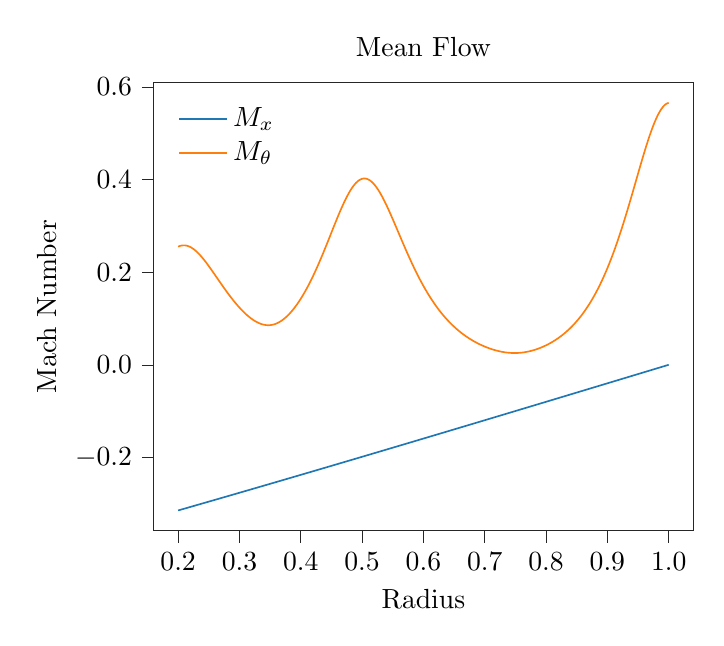
\begin{tikzpicture}

\definecolor{color0}{rgb}{0.12156862745098,0.466666666666667,0.705882352941177}
\definecolor{color1}{rgb}{1,0.498039215686275,0.0549019607843137}

\begin{axis}[
axis line style={white!15!black},
legend cell align={left},
legend style={
  fill opacity=0.8,
  draw opacity=1,
  text opacity=1,
  at={(0.03,0.97)},
  anchor=north west,
  draw=none
},
tick align=outside,
tick pos=left,
title={Mean Flow },
x grid style={white!80!black},
xlabel={Radius},
xmin=0.16, xmax=1.04,
xtick style={color=white!15!black},
xtick={0.1,0.2,0.3,0.4,0.5,0.6,0.7,0.8,0.9,1,1.1},
xticklabels={0.1,0.2,0.3,0.4,0.5,0.6,0.7,0.8,0.9,1.0,1.1},
y grid style={white!80!black},
ylabel={Mach Number},
ymin=-0.358579171685103, ymax=0.609698172253824,
ytick style={color=white!15!black},
ytick={-0.4,-0.2,0,0.2,0.4,0.6,0.8},
yticklabels={\ensuremath{-}0.4,\ensuremath{-}0.2,0.0,0.2,0.4,0.6,0.8}
]
\addplot [semithick, color0]
table {%
0.2 -0.314566565142425
0.2015625 -0.313973231598063
0.203125 -0.313379775407908
0.2046875 -0.312786196803778
0.20625 -0.31219249601754
0.2078125 -0.311598673281109
0.209375 -0.311004728826447
0.2109375 -0.310410662885563
0.2125 -0.309816475690513
0.2140625 -0.309222167473404
0.215625 -0.308627738466385
0.2171875 -0.308033188901657
0.21875 -0.307438519011464
0.2203125 -0.306843729028101
0.221875 -0.306248819183906
0.2234375 -0.305653789711266
0.225 -0.305058640842615
0.2265625 -0.304463372810433
0.228125 -0.303867985847246
0.2296875 -0.303272480185627
0.23125 -0.302676856058197
0.2328125 -0.302081113697619
0.234375 -0.301485253336607
0.2359375 -0.300889275207918
0.2375 -0.300293179544357
0.2390625 -0.299696966578772
0.240625 -0.29910063654406
0.2421875 -0.298504189673163
0.24375 -0.297907626199066
0.2453125 -0.297310946354804
0.246875 -0.296714150373453
0.2484375 -0.296117238488138
0.25 -0.295520210932026
0.2515625 -0.294923067938333
0.253125 -0.294325809740317
0.2546875 -0.293728436571281
0.25625 -0.293130948664575
0.2578125 -0.292533346253593
0.259375 -0.291935629571772
0.2609375 -0.291337798852597
0.2625 -0.290739854329594
0.2640625 -0.290141796236336
0.265625 -0.289543624806439
0.2671875 -0.288945340273564
0.26875 -0.288346942871416
0.2703125 -0.287748432833744
0.271875 -0.28714981039434
0.2734375 -0.286551075787042
0.275 -0.28595222924573
0.2765625 -0.285353271004329
0.278125 -0.284754201296807
0.2796875 -0.284155020357175
0.28125 -0.283555728419489
0.2828125 -0.282956325717846
0.284375 -0.282356812486389
0.2859375 -0.281757188959303
0.2875 -0.281157455370815
0.2890625 -0.280557611955196
0.290625 -0.27995765894676
0.2921875 -0.279357596579864
0.29375 -0.278757425088908
0.2953125 -0.278157144708332
0.296875 -0.277556755672622
0.2984375 -0.276956258216305
0.3 -0.27635565257395
0.3015625 -0.275754938980168
0.303125 -0.275154117669613
0.3046875 -0.274553188876981
0.30625 -0.273952152837011
0.3078125 -0.273351009784481
0.309375 -0.272749759954213
0.3109375 -0.27214840358107
0.3125 -0.271546940899957
0.3140625 -0.270945372145821
0.315625 -0.27034369755365
0.3171875 -0.269741917358471
0.31875 -0.269140031795357
0.3203125 -0.268538041099418
0.321875 -0.267935945505807
0.3234375 -0.267333745249717
0.325 -0.266731440566383
0.3265625 -0.266129031691081
0.328125 -0.265526518859126
0.3296875 -0.264923902305875
0.33125 -0.264321182266725
0.3328125 -0.263718358977114
0.334375 -0.263115432672518
0.3359375 -0.262512403588457
0.3375 -0.261909271960489
0.3390625 -0.261306038024212
0.340625 -0.260702702015264
0.3421875 -0.260099264169323
0.34375 -0.259495724722107
0.3453125 -0.258892083909374
0.346875 -0.258288341966921
0.3484375 -0.257684499130585
0.35 -0.257080555636242
0.3515625 -0.256476511719807
0.353125 -0.255872367617234
0.3546875 -0.255268123564519
0.35625 -0.254663779797693
0.3578125 -0.254059336552828
0.359375 -0.253454794066035
0.3609375 -0.252850152573463
0.3625 -0.252245412311301
0.3640625 -0.251640573515775
0.365625 -0.25103563642315
0.3671875 -0.25043060126973
0.36875 -0.249825468291857
0.3703125 -0.249220237725911
0.371875 -0.248614909808309
0.3734375 -0.248009484775508
0.375 -0.247403962864003
0.3765625 -0.246798344310325
0.378125 -0.246192629351044
0.3796875 -0.245586818222767
0.38125 -0.24498091116214
0.3828125 -0.244374908405845
0.384375 -0.243768810190601
0.3859375 -0.243162616753166
0.3875 -0.242556328330334
0.3890625 -0.241949945158937
0.390625 -0.241343467475843
0.3921875 -0.240736895517956
0.39375 -0.240130229522221
0.3953125 -0.239523469725615
0.396875 -0.238916616365153
0.3984375 -0.238309669677889
0.4 -0.23770262990091
0.4015625 -0.237095497271341
0.403125 -0.236488272026345
0.4046875 -0.235880954403117
0.40625 -0.235273544638891
0.4078125 -0.234666042970938
0.409375 -0.234058449636562
0.4109375 -0.233450764873104
0.4125 -0.232842988917941
0.4140625 -0.232235122008486
0.415625 -0.231627164382187
0.4171875 -0.231019116276527
0.41875 -0.230410977929025
0.4203125 -0.229802749577234
0.421875 -0.229194431458745
0.4234375 -0.228586023811182
0.425 -0.227977526872203
0.4265625 -0.227368940879503
0.428125 -0.226760266070811
0.4296875 -0.22615150268389
0.43125 -0.225542650956538
0.4328125 -0.224933711126589
0.434375 -0.224324683431909
0.4359375 -0.2237155681104
0.4375 -0.223106365399997
0.4390625 -0.222497075538671
0.440625 -0.221887698764424
0.4421875 -0.221278235315296
0.44375 -0.220668685429357
0.4453125 -0.220059049344713
0.446875 -0.219449327299504
0.4484375 -0.218839519531901
0.45 -0.21822962628011
0.4515625 -0.217619647782373
0.453125 -0.21700958427696
0.4546875 -0.21639943600218
0.45625 -0.215789203196369
0.4578125 -0.215178886097901
0.459375 -0.214568484945182
0.4609375 -0.213957999976648
0.4625 -0.21334743143077
0.4640625 -0.212736779546052
0.465625 -0.21212604456103
0.4671875 -0.211515226714272
0.46875 -0.210904326244379
0.4703125 -0.210293343389984
0.471875 -0.209682278389752
0.4734375 -0.209071131482379
0.475 -0.208459902906597
0.4765625 -0.207848592901165
0.478125 -0.207237201704876
0.4796875 -0.206625729556556
0.48125 -0.206014176695061
0.4828125 -0.205402543359278
0.484375 -0.204790829788126
0.4859375 -0.204179036220557
0.4875 -0.203567162895553
0.4890625 -0.202955210052125
0.490625 -0.202343177929319
0.4921875 -0.201731066766209
0.49375 -0.201118876801901
0.4953125 -0.200506608275533
0.496875 -0.19989426142627
0.4984375 -0.199281836493312
0.5 -0.198669333715887
0.5015625 -0.198056753333254
0.503125 -0.197444095584701
0.5046875 -0.196831360709549
0.50625 -0.196218548947147
0.5078125 -0.195605660536874
0.509375 -0.194992695718141
0.5109375 -0.194379654730386
0.5125 -0.193766537813078
0.5140625 -0.193153345205717
0.515625 -0.19254007714783
0.5171875 -0.191926733878976
0.51875 -0.191313315638742
0.5203125 -0.190699822666745
0.521875 -0.190086255202629
0.5234375 -0.18947261348607
0.525 -0.188858897756771
0.5265625 -0.188245108254466
0.528125 -0.187631245218915
0.5296875 -0.18701730888991
0.53125 -0.186403299507269
0.5328125 -0.185789217310838
0.534375 -0.185175062540495
0.5359375 -0.184560835436144
0.5375 -0.183946536237716
0.5390625 -0.183332165185173
0.540625 -0.182717722518503
0.5421875 -0.182103208477722
0.54375 -0.181488623302877
0.5453125 -0.180873967234038
0.546875 -0.180259240511305
0.5484375 -0.179644443374807
0.55 -0.179029576064698
0.5515625 -0.178414638821162
0.553125 -0.177799631884408
0.5546875 -0.177184555494672
0.55625 -0.17656940989222
0.5578125 -0.175954195317341
0.559375 -0.175338912010356
0.5609375 -0.174723560211609
0.5625 -0.17410814016147
0.5640625 -0.17349265210034
0.565625 -0.172877096268643
0.5671875 -0.17226147290683
0.56875 -0.17164578225538
0.5703125 -0.171030024554796
0.571875 -0.170414200045609
0.5734375 -0.169798308968375
0.575 -0.169182351563677
0.5765625 -0.168566328072123
0.578125 -0.167950238734347
0.5796875 -0.16733408379101
0.58125 -0.166717863482796
0.5828125 -0.166101578050417
0.584375 -0.165485227734609
0.5859375 -0.164868812776134
0.5875 -0.164252333415779
0.5890625 -0.163635789894357
0.590625 -0.163019182452705
0.5921875 -0.162402511331685
0.59375 -0.161785776772184
0.5953125 -0.161168979015113
0.596875 -0.160552118301411
0.5984375 -0.159935194872038
0.6 -0.159318208967979
0.6015625 -0.158701160830245
0.603125 -0.158084050699871
0.6046875 -0.157466878817914
0.60625 -0.156849645425458
0.6078125 -0.156232350763609
0.609375 -0.155614995073498
0.6109375 -0.154997578596281
0.6125 -0.154380101573134
0.6140625 -0.15376256424526
0.615625 -0.153144966853885
0.6171875 -0.152527309640257
0.61875 -0.151909592845649
0.6203125 -0.151291816711356
0.621875 -0.150673981478698
0.6234375 -0.150056087389016
0.625 -0.149438134683675
0.6265625 -0.148820123604062
0.628125 -0.14820205439159
0.6296875 -0.147583927287689
0.63125 -0.146965742533818
0.6328125 -0.146347500371453
0.634375 -0.145729201042096
0.6359375 -0.14511084478727
0.6375 -0.144492431848521
0.6390625 -0.143873962467415
0.640625 -0.143255436885543
0.6421875 -0.142636855344516
0.64375 -0.142018218085968
0.6453125 -0.141399525351553
0.646875 -0.140780777382949
0.6484375 -0.140161974421854
0.65 -0.139543116709988
0.6515625 -0.138924204489092
0.653125 -0.138305238000929
0.6546875 -0.137686217487282
0.65625 -0.137067143189957
0.6578125 -0.136448015350779
0.659375 -0.135828834211595
0.6609375 -0.135209600014273
0.6625 -0.134590313000702
0.6640625 -0.133970973412789
0.665625 -0.133351581492465
0.6671875 -0.13273213748168
0.66875 -0.132112641622403
0.6703125 -0.131493094156626
0.671875 -0.13087349532636
0.6734375 -0.130253845373634
0.675 -0.1296341445405
0.6765625 -0.129014393069028
0.678125 -0.12839459120131
0.6796875 -0.127774739179454
0.68125 -0.127154837245591
0.6828125 -0.12653488564187
0.684375 -0.125914884610459
0.6859375 -0.125294834393547
0.6875 -0.12467473523334
0.6890625 -0.124054587372064
0.690625 -0.123434391051966
0.6921875 -0.122814146515309
0.69375 -0.122193854004376
0.6953125 -0.121573513761469
0.696875 -0.120953126028908
0.6984375 -0.120332691049032
0.7 -0.1197122090642
0.7015625 -0.119091680316785
0.703125 -0.118471105049183
0.7046875 -0.117850483503806
0.70625 -0.117229815923084
0.7078125 -0.116609102549465
0.709375 -0.115988343625415
0.7109375 -0.115367539393419
0.7125 -0.114746690095978
0.7140625 -0.114125795975612
0.715625 -0.113504857274856
0.7171875 -0.112883874236266
0.71875 -0.112262847102412
0.7203125 -0.111641776115884
0.721875 -0.111020661519287
0.7234375 -0.110399503555244
0.725 -0.109778302466396
0.7265625 -0.109157058495398
0.728125 -0.108535771884924
0.7296875 -0.107914442877665
0.73125 -0.107293071716326
0.7328125 -0.106671658643631
0.734375 -0.10605020390232
0.7359375 -0.105428707735148
0.7375 -0.104807170384887
0.7390625 -0.104185592094326
0.740625 -0.103563973106267
0.7421875 -0.102942313663532
0.74375 -0.102320614008955
0.7453125 -0.101698874385389
0.746875 -0.1010770950357
0.7484375 -0.100455276202771
0.75 -0.0998334181294999
0.7515625 -0.0992115210587998
0.753125 -0.0985895852335994
0.7546875 -0.0979676108968424
0.75625 -0.0973455982914874
0.7578125 -0.0967235476605083
0.759375 -0.0961014592468934
0.7609375 -0.0954793332936462
0.7625 -0.0948571700437845
0.7640625 -0.0942349697403408
0.765625 -0.0936127326263622
0.7671875 -0.0929904589449099
0.76875 -0.0923681489390598
0.7703125 -0.0917458028519016
0.771875 -0.0911234209265392
0.7734375 -0.0905010034060907
0.775 -0.0898785505336877
0.7765625 -0.0892560625524761
0.778125 -0.0886335397056152
0.7796875 -0.0880109822362778
0.78125 -0.0873883903876507
0.7828125 -0.0867657644029336
0.784375 -0.0861431045253399
0.7859375 -0.0855204109980961
0.7875 -0.0848976840644419
0.7890625 -0.0842749239676299
0.790625 -0.0836521309509258
0.7921875 -0.0830293052576081
0.79375 -0.0824064471309682
0.7953125 -0.0817835568143099
0.796875 -0.0811606345509499
0.7984375 -0.0805376805842171
0.8 -0.0799146951574529
0.8015625 -0.079291678514011
0.803125 -0.0786686308972572
0.8046875 -0.0780455525505696
0.80625 -0.0774224437173381
0.8078125 -0.0767993046409646
0.809375 -0.0761761355648628
0.8109375 -0.0755529367324582
0.8125 -0.0749297083871877
0.8140625 -0.0743064507724999
0.815625 -0.0736831641318549
0.8171875 -0.073059848708724
0.81875 -0.0724365047465898
0.8203125 -0.071813132488946
0.821875 -0.0711897321792973
0.8234375 -0.0705663040611597
0.825 -0.0699428483780596
0.8265625 -0.0693193653735343
0.828125 -0.0686958552911321
0.8296875 -0.0680723183744114
0.83125 -0.0674487548669416
0.8328125 -0.0668251650123019
0.834375 -0.0662015490540821
0.8359375 -0.0655779072358824
0.8375 -0.0649542398013126
0.8390625 -0.0643305469939931
0.840625 -0.0637068290575537
0.8421875 -0.0630830862356343
0.84375 -0.0624593187718844
0.8453125 -0.0618355269099631
0.846875 -0.0612117108935392
0.8484375 -0.0605878709662909
0.85 -0.0599640073719054
0.8515625 -0.0593401203540797
0.853125 -0.0587162101565195
0.8546875 -0.0580922770229398
0.85625 -0.0574683211970645
0.8578125 -0.0568443429226261
0.859375 -0.0562203424433665
0.8609375 -0.0555963200030356
0.8625 -0.0549722758453923
0.8640625 -0.0543482102142038
0.865625 -0.0537241233532457
0.8671875 -0.0531000155063021
0.86875 -0.0524758869171648
0.8703125 -0.0518517378296344
0.871875 -0.0512275684875189
0.8734375 -0.0506033791346345
0.875 -0.0499791700148053
0.8765625 -0.0493549413718627
0.878125 -0.0487306934496463
0.8796875 -0.0481064264920028
0.88125 -0.0474821407427864
0.8828125 -0.0468578364458589
0.884375 -0.0462335138450891
0.8859375 -0.045609173184353
0.8875 -0.0449848147075337
0.8890625 -0.0443604386585211
0.890625 -0.0437360452812123
0.8921875 -0.0431116348195108
0.89375 -0.042487207517327
0.8953125 -0.0418627636185779
0.896875 -0.0412383033671867
0.8984375 -0.0406138270070833
0.9 -0.0399893347822038
0.9015625 -0.0393648269364904
0.903125 -0.0387403037138917
0.9046875 -0.0381157653583617
0.90625 -0.037491212113861
0.9078125 -0.0368666442243555
0.909375 -0.0362420619338172
0.9109375 -0.0356174654862236
0.9125 -0.0349928551255574
0.9140625 -0.0343682310958073
0.915625 -0.0337435936409669
0.9171875 -0.0331189430050354
0.91875 -0.0324942794320168
0.9203125 -0.0318696031659202
0.921875 -0.03124491445076
0.9234375 -0.0306202135305551
0.925 -0.0299955006493293
0.9265625 -0.0293707760511112
0.928125 -0.0287460399799336
0.9296875 -0.0281212926798342
0.93125 -0.0274965343948549
0.9328125 -0.0268717653690419
0.934375 -0.0262469858464456
0.9359375 -0.0256221960711204
0.9375 -0.024997396287125
0.9390625 -0.0243725867385215
0.940625 -0.0237477676693765
0.9421875 -0.0231229393237598
0.94375 -0.0224981019457448
0.9453125 -0.0218732557794089
0.946875 -0.0212484010688324
0.9484375 -0.0206235380580993
0.95 -0.0199986669912967
0.9515625 -0.0193737881125147
0.953125 -0.0187489016658469
0.9546875 -0.0181240078953893
0.95625 -0.0174991070452412
0.9578125 -0.0168741993595044
0.959375 -0.0162492850822834
0.9609375 -0.0156243644576856
0.9625 -0.0149994377298203
0.9640625 -0.0143745051427998
0.965625 -0.0137495669407382
0.9671875 -0.0131246233677519
0.96875 -0.0124996746679598
0.9703125 -0.0118747210854821
0.971875 -0.0112497628644416
0.9734375 -0.0106248002489625
0.975 -0.00999983348317079
0.9765625 -0.00937486281119418
0.978125 -0.00874988847716171
0.9796875 -0.00812491072520414
0.98125 -0.00749992979945334
0.9828125 -0.00687494594404237
0.984375 -0.00624995940310574
0.9859375 -0.00562497042077864
0.9875 -0.00499997924119756
0.9890625 -0.0043749861084996
0.990625 -0.00374999126682261
0.9921875 -0.00312499496030536
0.99375 -0.00249999743308688
0.9953125 -0.00187499892930699
0.996875 -0.00124999969310565
0.9984375 -0.000624999968623085
1 0
};
\addlegendentry{$M_{x}$}
\addplot [semithick, color1]
table {%
0.2 0.255065159843046
0.2015625 0.255968364411969
0.203125 0.256706833358219
0.2046875 0.257279572376127
0.20625 0.257686110072619
0.2078125 0.257926497257104
0.209375 0.258001302302394
0.2109375 0.257911602675627
0.2125 0.257658972790116
0.2140625 0.257245468377284
0.215625 0.256673607621338
0.2171875 0.255946349337276
0.21875 0.255067068504603
0.2203125 0.254039529494257
0.221875 0.25286785734447
0.2234375 0.251556507452602
0.225 0.250110234054432
0.2265625 0.248534057860345
0.228125 0.246833233209701
0.2296875 0.245013215091013
0.23125 0.243079626357068
0.2328125 0.241038225441498
0.234375 0.238894874857357
0.2359375 0.236655510729794
0.2375 0.234326113584628
0.2390625 0.231912680583411
0.240625 0.229421199363994
0.2421875 0.226857623614387
0.24375 0.224227850477382
0.2453125 0.221537699854474
0.246875 0.218792895650435
0.2484375 0.21599904897482
0.25 0.21316164329395
0.2515625 0.210286021506594
0.253125 0.207377374898871
0.2546875 0.204440733918698
0.25625 0.201480960697466
0.2578125 0.198502743236421
0.259375 0.19551059116732
0.2609375 0.192508832991191
0.2625 0.189501614695225
0.2640625 0.186492899645885
0.265625 0.183486469655856
0.2671875 0.180485927123467
0.26875 0.177494698145321
0.2703125 0.174516036506022
0.271875 0.171553028452757
0.2734375 0.168608598167034
0.275 0.165685513850817
0.2765625 0.162786394349561
0.278125 0.159913716240034
0.2796875 0.157069821316225
0.28125 0.154256924411978
0.2828125 0.151477121504055
0.284375 0.148732398044197
0.2859375 0.146024637473106
0.2875 0.143355629873271
0.2890625 0.140727080720902
0.290625 0.138140619700031
0.2921875 0.13559780954393
0.29375 0.133100154870287
0.2953125 0.130649110977115
0.296875 0.128246092566015
0.2984375 0.125892482358112
0.3 0.123589639565741
0.3015625 0.121338908179735
0.303125 0.119141625027891
0.3046875 0.116999127554962
0.30625 0.114912761268305
0.3078125 0.112883886786253
0.309375 0.110913886418458
0.3109375 0.109004170199123
0.3125 0.107156181285485
0.3140625 0.105371400625434
0.315625 0.103651350790409
0.3171875 0.1019975988631
0.31875 0.100411758264908
0.3203125 0.0988954894063168
0.321875 0.0974504990452432
0.3234375 0.0960785382451227
0.325 0.0947813988368702
0.3265625 0.0935609083079101
0.328125 0.0924189230679663
0.3296875 0.0913573200756757
0.33125 0.0903779868524443
0.3328125 0.089482809959776
0.334375 0.0886736620724435
0.3359375 0.0879523878403873
0.3375 0.0873207887944687
0.3390625 0.0867806076117272
0.340625 0.0863335121106115
0.3421875 0.085981079391489
0.34375 0.085724780568301
0.3453125 0.0855659665497199
0.346875 0.0855058553197153
0.3484375 0.0855455211364491
0.35 0.0856858860149973
0.3515625 0.0859277137854266
0.353125 0.0862716069268763
0.3546875 0.0867180062757169
0.35625 0.0872671935977731
0.3578125 0.0879192969077789
0.359375 0.0886742983202184
0.3609375 0.089532044130272
0.3625 0.0904922567562133
0.3640625 0.0915545481281322
0.365625 0.0927184340833403
0.3671875 0.0939833493256452
0.36875 0.0953486625217281
0.3703125 0.0968136911400023
0.371875 0.0983777156816692
0.3734375 0.100039993006174
0.375 0.101799768509913
0.3765625 0.103656286974313
0.378125 0.105608801954347
0.3796875 0.107656583628954
0.38125 0.109798925079123
0.3828125 0.112035146996802
0.384375 0.11436460085794
0.3859375 0.116786670616132
0.3875 0.1193007729899
0.3890625 0.121906356427498
0.390625 0.124602898838949
0.3921875 0.127389904186897
0.39375 0.130266898026433
0.3953125 0.133233422080402
0.396875 0.136289027931298
0.3984375 0.139433269904513
0.4 0.142665697210859
0.4015625 0.145985845409386
0.403125 0.149393227244884
0.4046875 0.152887322908421
0.40625 0.156467569763883
0.4078125 0.160133351579076
0.409375 0.163883987296415
0.4109375 0.167718719375798
0.4125 0.171636701740867
0.4140625 0.175636987359539
0.415625 0.179718515490483
0.4171875 0.183880098629044
0.41875 0.188120409189027
0.4203125 0.192437965960647
0.421875 0.196831120389881
0.4234375 0.201298042730311
0.425 0.205836708125276
0.4265625 0.210444882685797
0.428125 0.215120109638081
0.4296875 0.219859695623494
0.43125 0.224660697243575
0.4328125 0.229519907952808
0.434375 0.234433845412387
0.4359375 0.239398739428929
0.4375 0.244410520612798
0.4390625 0.249464809901279
0.440625 0.254556909101945
0.4421875 0.259681792621032
0.44375 0.264834100550136
0.4453125 0.27000813329177
0.446875 0.275197847909978
0.4484375 0.280396856395864
0.45 0.285598426039319
0.4515625 0.290795482096905
0.453125 0.295980612941552
0.4546875 0.301146077871998
0.45625 0.306283817748479
0.4578125 0.31138546860576
0.459375 0.316442378374904
0.4609375 0.32144562682116
0.4625 0.326386048776775
0.4640625 0.331254260714544
0.465625 0.336040690670567
0.4671875 0.340735611483277
0.46875 0.345329177270684
0.4703125 0.349811463019533
0.471875 0.35417250710938
0.4734375 0.358402356542188
0.475 0.362491114595036
0.4765625 0.366428990560886
0.478125 0.370206351191277
0.4796875 0.37381377340661
0.48125 0.377242097795612
0.4828125 0.380482482386889
0.484375 0.383526456143579
0.4859375 0.386365971608016
0.4875 0.388993456108193
0.4890625 0.391401860932495
0.490625 0.393584707884263
0.4921875 0.395536132643813
0.49375 0.397250924392459
0.4953125 0.398724561190988
0.496875 0.399953240653146
0.4984375 0.400933905512442
0.5 0.401664263746783
0.5015625 0.402142802998784
0.503125 0.402368799108529
0.5046875 0.402342318658297
0.50625 0.402064215513529
0.5078125 0.401536121429045
0.509375 0.400760430872516
0.5109375 0.399740280296358
0.5125 0.398479522163042
0.5140625 0.396982694095653
0.515625 0.395254983584066
0.5171875 0.39330218872638
0.51875 0.391130675524381
0.5203125 0.388747332280452
0.521875 0.386159521661241
0.5234375 0.383375031000781
0.525 0.380402021412906
0.5265625 0.37724897627048
0.528125 0.373924649587917
0.5296875 0.370438014814742
0.53125 0.366798214512707
0.5328125 0.363014511348306
0.534375 0.359096240787847
0.5359375 0.355052765834596
0.5375 0.350893434098191
0.5390625 0.346627537436659
0.540625 0.342264274361892
0.5421875 0.337812715351385
0.54375 0.333281771163073
0.5453125 0.328680164206925
0.546875 0.324016402987131
0.5484375 0.319298759592463
0.55 0.314535250180197
0.5515625 0.309733618370758
0.553125 0.304901321446166
0.5546875 0.300045519225358
0.55625 0.295173065473267
0.5578125 0.290290501688204
0.559375 0.285404053103047
0.5609375 0.280519626730042
0.5625 0.275642811276067
0.5640625 0.27077887875488
0.565625 0.265932787624734
0.5671875 0.261109187283532
0.56875 0.256312423759043
0.5703125 0.251546546438397
0.571875 0.246815315688742
0.5734375 0.242122211229442
0.575 0.237470441125182
0.5765625 0.232862951278719
0.578125 0.22830243531152
0.5796875 0.223791344730069
0.58125 0.219331899285021
0.5828125 0.21492609743956
0.584375 0.210575726872192
0.5859375 0.206282374947681
0.5875 0.202047439097858
0.5890625 0.197872137061639
0.590625 0.193757516940619
0.5921875 0.189704467033205
0.59375 0.185713725416266
0.5953125 0.181785889248833
0.596875 0.177921423777413
0.5984375 0.174120671027024
0.6 0.170383858166168
0.6015625 0.166711105537592
0.603125 0.163102434349923
0.6046875 0.159557774028135
0.60625 0.156076969223248
0.6078125 0.152659786483873
0.609375 0.149305920594004
0.6109375 0.146015000583079
0.6125 0.142786595415612
0.6140625 0.139620219368809
0.615625 0.136515337107451
0.6171875 0.13347136846603
0.61875 0.130487692948654
0.6203125 0.12756365395764
0.621875 0.124698562761982
0.6234375 0.121891702217005
0.625 0.119142330246641
0.6265625 0.116449683099675
0.628125 0.113812978391277
0.6296875 0.11123141794095
0.63125 0.108704190417859
0.6328125 0.106230473804262
0.634375 0.103809437687483
0.6359375 0.101440245390631
0.6375 0.0991220559518919
0.6390625 0.0968540259619605
0.640625 0.0946353112688321
0.6421875 0.092465068558833
0.64375 0.0903424568224584
0.6453125 0.088266638713247
0.646875 0.0862367818075993
0.6484375 0.0842520597731427
0.65 0.0823116534529223
0.6515625 0.0804147518724195
0.653125 0.0785605531761026
0.6546875 0.0767482654999489
0.65625 0.074977107786117
0.6578125 0.0732463105456957
0.659375 0.07155511657523
0.6609375 0.0699027816324986
0.6625 0.0682885750768002
0.6640625 0.0667117804788219
0.665625 0.0651716962049498
0.6671875 0.063667635980726
0.66875 0.0621989294379548
0.6703125 0.0607649226497941
0.671875 0.059364978658023
0.6734375 0.0579984779964363
0.675 0.0566648192142266
0.6765625 0.0553634194029264
0.678125 0.0540937147303553
0.6796875 0.0528551609847307
0.68125 0.0516472341318674
0.6828125 0.0504694308880978
0.684375 0.0493212693111629
0.6859375 0.0482022894109793
0.6875 0.0471120537816698
0.6890625 0.0460501482556922
0.690625 0.0450161825803071
0.6921875 0.0440097911157661
0.69375 0.043030633553821
0.6953125 0.0420783956540049
0.696875 0.0411527899940301
0.6984375 0.0402535567291964
0.7 0.0393804643541552
0.7015625 0.0385333104585603
0.703125 0.0377119224661578
0.7046875 0.0369161583445847
0.70625 0.03614590727077
0.7078125 0.0354010902341206
0.709375 0.0346816605569391
0.7109375 0.0339876043086025
0.7125 0.0333189405871274
0.7140625 0.032675721638941
0.715625 0.0320580327850901
0.7171875 0.0314659921199864
0.71875 0.030899749947283
0.7203125 0.0303594879168096
0.721875 0.0298454178271658
0.7234375 0.0293577800605058
0.725 0.028896841619993
0.7265625 0.02846289374629
0.728125 0.0280562490976937
0.7296875 0.0276772384892812
0.73125 0.0273262071995499
0.7328125 0.0270035108686346
0.734375 0.0267095110295417
0.7359375 0.0264445703327243
0.7375 0.0262090475435282
0.7390625 0.0260032924107508
0.740625 0.0258276405213213
0.7421875 0.0256824082697078
0.74375 0.025567888079597
0.7453125 0.0254843440186413
0.746875 0.02543200794361
0.7484375 0.0254110763027492
0.75 0.0254217077045359
0.7515625 0.0254640213381115
0.753125 0.0255380963015776
0.7546875 0.0256439718618399
0.75625 0.0257816486357861
0.7578125 0.0259510906494439
0.759375 0.0261522282015027
0.7609375 0.0263849614319338
0.7625 0.0266491644768043
0.7640625 0.0269446900775945
0.765625 0.0272713745074708
0.7671875 0.0276290426780044
0.76875 0.0280175132966183
0.7703125 0.0284366039568782
0.771875 0.0288861360590011
0.7734375 0.0293659394755854
0.775 0.0298758568960128
0.7765625 0.030415747801474
0.778125 0.0309854920398314
0.7796875 0.0315849929852943
0.78125 0.0322141802813672
0.7828125 0.0328730121767872
0.784375 0.0335614774730271
0.7859375 0.0342795971084747
0.7875 0.0350274254090058
0.7890625 0.0358050510372605
0.790625 0.0366125976742192
0.7921875 0.0374502244665543
0.79375 0.0383181262722576
0.7953125 0.0392165337353146
0.796875 0.040145713218003
0.7984375 0.0411059666168876
0.8 0.0420976310859398
0.8015625 0.0431210786874706
0.803125 0.0441767159889997
0.8046875 0.0452649836215835
0.80625 0.0463863558127949
0.8078125 0.0475413399053534
0.809375 0.0487304758704063
0.8109375 0.0499543358226658
0.8125 0.0512135235430355
0.8140625 0.0525086740128872
0.815625 0.0538404529629672
0.8171875 0.0552095564387755
0.81875 0.0566167103833332
0.8203125 0.0580626702374222
0.821875 0.0595482205566574
0.8234375 0.0610741746441408
0.825 0.062641374196886
0.8265625 0.0642506889637268
0.828125 0.0659030164120159
0.8296875 0.067599281400005
0.83125 0.0693404358514907
0.8328125 0.0711274584289652
0.834375 0.0729613542012303
0.8359375 0.07484315430113
0.8375 0.0767739155687956
0.8390625 0.0787547201755158
0.840625 0.0807866752230513
0.8421875 0.0828709123129645
0.84375 0.0850085870801981
0.8453125 0.0872008786848752
0.846875 0.0894489892559412
0.8484375 0.0917541432799597
0.85 0.0941175869280004
0.8515625 0.0965405873132023
0.853125 0.0990244316711992
0.8546875 0.101570426455177
0.85625 0.104179896336902
0.8578125 0.106854183104609
0.859375 0.109594644448144
0.8609375 0.112402652621281
0.8625 0.115279592970591
0.8640625 0.118226862319719
0.865625 0.121245867197353
0.8671875 0.124338021896614
0.86875 0.127504746353011
0.8703125 0.130747463827489
0.871875 0.134067598380528
0.8734375 0.13746657212265
0.875 0.14094580222606
0.8765625 0.144506697681637
0.878125 0.148150655784842
0.8796875 0.151879058333667
0.88125 0.15569326752118
0.8828125 0.159594621504825
0.884375 0.163584429634248
0.8859375 0.167663967319096
0.8875 0.171834470518073
0.8890625 0.176097129830408
0.890625 0.180453084170948
0.8921875 0.184903414010309
0.89375 0.189449134161866
0.8953125 0.194091186097979
0.896875 0.198830429778696
0.8984375 0.203667634977241
0.9 0.208603472088054
0.9015625 0.213638502404859
0.903125 0.218773167858416
0.9046875 0.22400778020613
0.90625 0.229342509668755
0.9078125 0.234777373012944
0.909375 0.24031222108247
0.9109375 0.245946725785683
0.9125 0.251680366552035
0.9140625 0.25751241627655
0.915625 0.263441926777863
0.9171875 0.269467713802905
0.91875 0.275588341619623
0.9203125 0.281802107248194
0.921875 0.288107024391076
0.9234375 0.294500807132996
0.925 0.300980853493419
0.9265625 0.307544228926396
0.928125 0.314187649875617
0.9296875 0.320907467506142
0.93125 0.327699651748462
0.9328125 0.334559775805034
0.934375 0.341483001284309
0.9359375 0.348464064142019
0.9375 0.355497261624187
0.9390625 0.36257644042046
0.940625 0.369694986249733
0.9421875 0.376845815112347
0.94375 0.384021366453792
0.9453125 0.391213598493737
0.946875 0.398413985980555
0.9484375 0.405613520635077
0.95 0.412802714547513
0.9515625 0.419971606787799
0.953125 0.427109773481643
0.9546875 0.434206341591764
0.95625 0.44125000662576
0.9578125 0.448229054468482
0.959375 0.455131387507252
0.9609375 0.461944555182711
0.9625 0.468655789056426
0.9640625 0.475252042438538
0.965625 0.481720034565212
0.9671875 0.488046299256582
0.96875 0.494217237922058
0.9703125 0.500219176712006
0.971875 0.506038427543904
0.9734375 0.511661352658388
0.975 0.517074432287396
0.9765625 0.522264334944558
0.978125 0.527217989778637
0.9796875 0.531922660365945
0.98125 0.536366019259179
0.9828125 0.540536222559617
0.984375 0.544421983739021
0.9859375 0.548012645908313
0.9875 0.55129825171366
0.9890625 0.554269610038046
0.990625 0.556918358698616
0.9921875 0.559237022357485
0.99375 0.561219064906353
0.9953125 0.562858935642828
0.996875 0.564152108628062
0.9984375 0.565095114699835
1 0.565685565711145
};
\addlegendentry{$M_{\theta}$}
\end{axis}

\end{tikzpicture}

    \end{center}
\end{figure}

\begin{figure}
    \begin{center}
        % This file was created with tikzplotlib v0.9.12.
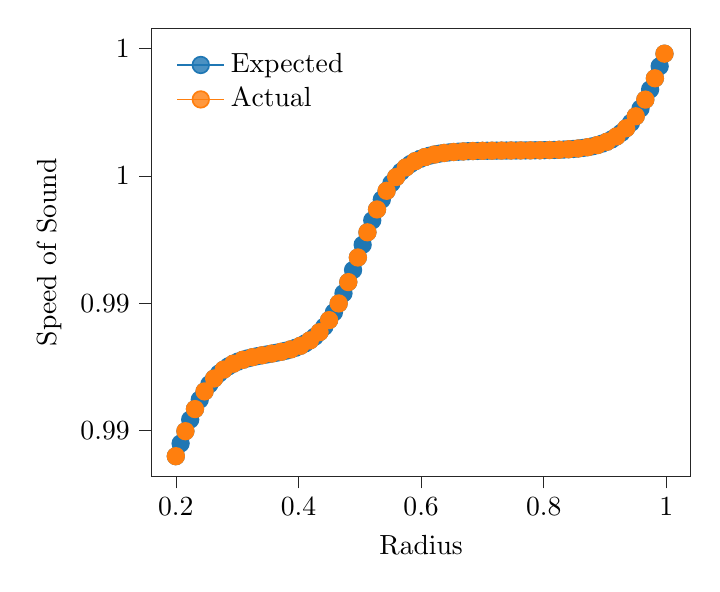
\begin{tikzpicture}

\definecolor{color0}{rgb}{0.12156862745098,0.466666666666667,0.705882352941177}
\definecolor{color1}{rgb}{1,0.498039215686275,0.0549019607843137}

\begin{axis}[
axis line style={white!15!black},
legend cell align={left},
legend style={
  fill opacity=0.8,
  draw opacity=1,
  text opacity=1,
  at={(0.03,0.97)},
  anchor=north west,
  draw=none
},
tick align=outside,
tick pos=left,
x grid style={white!80!black},
xlabel={Radius},
xmin=0.16, xmax=1.04,
xtick style={color=white!15!black},
y grid style={white!80!black},
ylabel={Speed of Sound},
ymin=0.98320056903035, ymax=1.00079997290332,
ytick style={color=white!15!black}
]
\addplot [semithick, color0, mark=*, mark size=3, mark repeat=5, mark options={solid}]
table {%
0.2 0.984000541933667
0.2015625 0.984100548886647
0.203125 0.984200432419622
0.2046875 0.984300068384446
0.20625 0.984399333875707
0.2078125 0.984498107834061
0.209375 0.984596271630271
0.2109375 0.984693709624082
0.2125 0.984790309692462
0.2140625 0.984885963722324
0.215625 0.984980568063398
0.2171875 0.985074023937652
0.21875 0.985166237802302
0.2203125 0.985257121664242
0.221875 0.985346593344428
0.2234375 0.985434576691501
0.225 0.985521001744648
0.2265625 0.985605804846342
0.228125 0.985688928706271
0.2296875 0.985770322418282
0.23125 0.985849941432696
0.2328125 0.985927747486754
0.234375 0.986003708496322
0.2359375 0.986077798412233
0.2375 0.986149997044859
0.2390625 0.986220289860638
0.240625 0.986288667754308
0.2421875 0.986355126800626
0.24375 0.986419667989276
0.2453125 0.986482296946548
0.246875 0.986543023647233
0.2484375 0.986601862119971
0.25 0.986658830149088
0.2515625 0.986713948975696
0.253125 0.98676724300061
0.2546875 0.98681873949133
0.25625 0.986868468295113
0.2578125 0.986916461559873
0.259375 0.986962753464396
0.2609375 0.987007379959106
0.2625 0.987050378518398
0.2640625 0.987091787905317
0.265625 0.987131647949157
0.2671875 0.987169999336396
0.26875 0.98720688341517
0.2703125 0.987242342013376
0.271875 0.987276417270339
0.2734375 0.987309151481869
0.275 0.987340586958444
0.2765625 0.987370765896143
0.278125 0.987399730259926
0.2796875 0.987427521678759
0.28125 0.987454181352077
0.2828125 0.987479749967015
0.284375 0.987504267625839
0.2859375 0.987527773782981
0.2875 0.987550307191088
0.2890625 0.987571905855486
0.290625 0.987592606996474
0.2921875 0.987612447018872
0.29375 0.987631461488276
0.2953125 0.987649685113462
0.296875 0.987667151734442
0.2984375 0.987683894315661
0.3 0.987699944943884
0.3015625 0.987715334830319
0.303125 0.987730094316565
0.3046875 0.987744252883996
0.30625 0.987757839166223
0.3078125 0.987770880964282
0.309375 0.987783405264264
0.3109375 0.987795438257075
0.3125 0.987807005360076
0.3140625 0.987818131240364
0.315625 0.987828839839472
0.3171875 0.987839154399291
0.31875 0.98784909748904
0.3203125 0.987858691033117
0.321875 0.9878679563397
0.3234375 0.987876914129958
0.325 0.987885584567766
0.3265625 0.987893987289837
0.328125 0.98790214143616
0.3296875 0.987910065680699
0.33125 0.987917778262275
0.3328125 0.987925297015572
0.334375 0.987932639402246
0.3359375 0.987939822542074
0.3375 0.987946863244137
0.3390625 0.987953778037998
0.340625 0.987960583204877
0.3421875 0.987967294808789
0.34375 0.98797392872766
0.3453125 0.987980500684408
0.346875 0.987987026277992
0.3484375 0.987993521014427
0.35 0.988000000337782
0.3515625 0.988006479661155
0.353125 0.988012974397646
0.3546875 0.988019499991323
0.35625 0.988026071948201
0.3578125 0.988032705867241
0.359375 0.988039417471358
0.3609375 0.988046222638482
0.3625 0.988053137432628
0.3640625 0.988060178135015
0.365625 0.988067361275209
0.3671875 0.98807470366229
0.36875 0.988082222416037
0.3703125 0.988089934998106
0.371875 0.988097859243185
0.3734375 0.988106013390094
0.375 0.988114416112798
0.3765625 0.988123086551289
0.378125 0.988132044342281
0.3796875 0.988141309649652
0.38125 0.988150903194572
0.3828125 0.98816084628522
0.384375 0.988171160845998
0.3859375 0.988181869446127
0.3875 0.9881929953275
0.3890625 0.988204562431654
0.390625 0.988216595425687
0.3921875 0.988229119726965
0.39375 0.988242161526395
0.3953125 0.988255747810073
0.396875 0.988269906379039
0.3984375 0.988284665866907
0.4 0.988300055755055
0.4015625 0.988316106385087
0.403125 0.988332848968214
0.4046875 0.988350315591207
0.40625 0.988368539218517
0.4078125 0.988387553690159
0.409375 0.988407393714916
0.4109375 0.988428094858389
0.4125 0.988449693525406
0.4140625 0.988472226936272
0.415625 0.988495733096318
0.4171875 0.988520250758199
0.41875 0.988545819376356
0.4203125 0.988572479053063
0.421875 0.988600270475462
0.4234375 0.988629234842998
0.425 0.988659413784646
0.4265625 0.988690849265375
0.428125 0.988723583481276
0.4296875 0.988757658742837
0.43125 0.98879311734588
0.4328125 0.988830001429742
0.434375 0.988868352822332
0.4359375 0.9889082128718
0.4375 0.988949622264638
0.4390625 0.988992620830155
0.440625 0.989037247331411
0.4421875 0.989083539242818
0.44375 0.989131532514817
0.4453125 0.989181261326212
0.446875 0.989232757824935
0.4484375 0.989286051858266
0.45 0.989341170693724
0.4515625 0.989398138732145
0.453125 0.989456977214666
0.4546875 0.989517703925637
0.45625 0.989580332893724
0.4578125 0.989644874093744
0.459375 0.989711333152017
0.4609375 0.989779711058255
0.4625 0.989850003887249
0.4640625 0.989922202533768
0.465625 0.989996292464284
0.4671875 0.990072253489208
0.46875 0.99015005955941
0.4703125 0.990229678590797
0.471875 0.990311072320652
0.4734375 0.99039419619934
0.475 0.990478999320756
0.4765625 0.990565424394636
0.478125 0.990653407763507
0.4796875 0.990742879466609
0.48125 0.99083376335264
0.4828125 0.990925977242617
0.484375 0.991019433143496
0.4859375 0.991114037512562
0.4875 0.991209691571851
0.4890625 0.991306291671168
0.490625 0.991403729697502
0.4921875 0.991501893527903
0.49375 0.991600667522201
0.4953125 0.99169993305125
0.496875 0.991799569055799
0.4984375 0.991899452630537
0.5 0.991999459627421
0.5015625 0.992099465272067
0.503125 0.99219934478671
0.5046875 0.992298974013166
0.50625 0.992398230029186
0.5078125 0.992496991751752
0.509375 0.992595140521059
0.5109375 0.992692560659307
0.5125 0.992789139998857
0.5140625 0.99288477037483
0.515625 0.992979348077864
0.5171875 0.99307277426338
0.51875 0.993164955314424
0.5203125 0.993255803155917
0.521875 0.993345235518834
0.5234375 0.993433176153603
0.525 0.993519554992716
0.5265625 0.993604308263212
0.528125 0.993687378550314
0.5296875 0.993768714814062
0.53125 0.993848272361297
0.5328125 0.993926012775751
0.534375 0.994001903809366
0.5359375 0.99407591923823
0.5375 0.994148038686721
0.5390625 0.99421824742356
0.540625 0.994286536133559
0.5421875 0.994352900668823
0.54375 0.994417341783093
0.5453125 0.994479864852854
0.546875 0.994540479588594
0.5484375 0.994599199739509
0.55 0.994656042794637
0.5515625 0.994711029683234
0.553125 0.994764184476907
0.5546875 0.994815534095789
0.55625 0.994865108020749
0.5578125 0.99491293801338
0.559375 0.99495905784526
0.5609375 0.995003503037712
0.5625 0.995046310613072
0.5640625 0.995087518858254
0.565625 0.995127167101171
0.5671875 0.995165295500434
0.56875 0.99520194484852
0.5703125 0.995237156388507
0.571875 0.995270971644298
0.5734375 0.995303432264168
0.575 0.995334579877347
0.5765625 0.995364455963282
0.578125 0.995393101733155
0.5796875 0.995420558023162
0.58125 0.995446865199025
0.5828125 0.995472063071189
0.584375 0.9954961908201
0.5859375 0.995519286930997
0.5875 0.995541389137587
0.5890625 0.995562534374025
0.590625 0.995582758734604
0.5921875 0.995602097440566
0.59375 0.995620584813474
0.5953125 0.995638254254612
0.596875 0.995655138229866
0.5984375 0.995671268259608
0.6 0.995686674913096
0.6015625 0.995701387806942
0.603125 0.995715435607232
0.6046875 0.995728846034892
0.60625 0.99574164587393
0.6078125 0.995753860982223
0.609375 0.995765516304507
0.6109375 0.995776635887292
0.6125 0.995787242895424
0.6140625 0.995797359630043
0.615625 0.995807007547711
0.6171875 0.995816207280501
0.61875 0.995824978656858
0.6203125 0.995833340723064
0.621875 0.995841311765143
0.6234375 0.995848909331092
0.625 0.995856150253272
0.6265625 0.995863050670899
0.628125 0.995869626052497
0.6296875 0.99587589121825
0.63125 0.995881860362164
0.6328125 0.995887547073985
0.634375 0.995892964360806
0.6359375 0.995898124668321
0.6375 0.995903039901678
0.6390625 0.995907721445908
0.640625 0.995912180185882
0.6421875 0.995916426525794
0.64375 0.995920470408134
0.6453125 0.995924321332153
0.646875 0.995927988371789
0.6484375 0.995931480193072
0.65 0.995934805070983
0.6515625 0.995937970905779
0.653125 0.99594098523878
0.6546875 0.995943855267619
0.65625 0.995946587860976
0.6578125 0.995949189572774
0.659375 0.995951666655872
0.6609375 0.995954025075258
0.6625 0.99595627052074
0.6640625 0.995958408419154
0.665625 0.995960443946116
0.6671875 0.995962382037296
0.66875 0.995964227399259
0.6703125 0.995965984519872
0.671875 0.995967657678284
0.6734375 0.995969250954509
0.675 0.995970768238611
0.6765625 0.995972213239507
0.678125 0.995973589493407
0.6796875 0.995974900371901
0.68125 0.995976149089699
0.6828125 0.995977338712054
0.684375 0.995978472161855
0.6859375 0.995979552226434
0.6875 0.995980581564065
0.6890625 0.995981562710198
0.690625 0.995982498083416
0.6921875 0.995983389991139
0.69375 0.995984240635083
0.6953125 0.995985052116483
0.696875 0.995985826441091
0.6984375 0.99598656552396
0.7 0.995987271194022
0.7015625 0.995987945198473
0.703125 0.995988589206969
0.7046875 0.995989204815643
0.70625 0.995989793550959
0.7078125 0.995990356873398
0.709375 0.995990896180996
0.7109375 0.99599141281273
0.7125 0.99599190805178
0.7140625 0.99599238312864
0.715625 0.995992839224128
0.7171875 0.995993277472259
0.71875 0.995993698963021
0.7203125 0.99599410474504
0.721875 0.99599449582815
0.7234375 0.995994873185871
0.725 0.995995237757798
0.7265625 0.995995590451909
0.728125 0.995995932146805
0.7296875 0.995996263693868
0.73125 0.995996585919359
0.7328125 0.995996899626465
0.734375 0.995997205597271
0.7359375 0.9959975045947
0.7375 0.995997797364393
0.7390625 0.995998084636562
0.740625 0.995998367127788
0.7421875 0.995998645542801
0.74375 0.995998920576223
0.7453125 0.995999192914293
0.746875 0.995999463236562
0.7484375 0.995999732217585
0.75 0.996000000528589
0.7515625 0.996000268839138
0.753125 0.996000537818796
0.7546875 0.996000808138787
0.75625 0.996001080473659
0.7578125 0.996001355502957
0.759375 0.996001633912908
0.7609375 0.996001916398121
0.7625 0.996002203663312
0.7640625 0.996002496425045
0.765625 0.996002795413511
0.7671875 0.996003101374329
0.76875 0.996003415070396
0.7703125 0.996003737283773
0.771875 0.996004068817611
0.7734375 0.996004410498143
0.775 0.996004763176713
0.7765625 0.996005127731883
0.778125 0.996005505071589
0.7796875 0.996005896135382
0.78125 0.996006301896732
0.7828125 0.996006723365422
0.784375 0.996007161590024
0.7859375 0.996007617660467
0.7875 0.996008092710702
0.7890625 0.996008587921481
0.790625 0.996009104523228
0.7921875 0.996009643799046
0.79375 0.996010207087836
0.7953125 0.996010795787547
0.796875 0.996011411358571
0.7984375 0.996012055327279
0.8 0.996012729289704
0.8015625 0.996013434915398
0.803125 0.996014173951444
0.8046875 0.996014948226658
0.80625 0.99601575965597
0.8078125 0.996016610245002
0.809375 0.99601750209485
0.8109375 0.996018437407087
0.8125 0.996019418488979
0.8140625 0.99602044775895
0.815625 0.996021527752279
0.8171875 0.996022661127064
0.81875 0.996023850670446
0.8203125 0.996025099305121
0.821875 0.99602641009613
0.8234375 0.996027786257968
0.825 0.996029231161992
0.8265625 0.996030748344171
0.828125 0.996032341513167
0.8296875 0.996034014558775
0.83125 0.996035771560727
0.8328125 0.996037616797878
0.834375 0.996039554757779
0.8359375 0.996041590146669
0.8375 0.996043727899874
0.8390625 0.996045973192643
0.840625 0.996048331451433
0.8421875 0.996050808365651
0.84375 0.99605340989986
0.8453125 0.996056142306476
0.846875 0.996059012138958
0.8484375 0.99606202626549
0.85 0.996065191883192
0.8515625 0.996068516532841
0.853125 0.996072008114122
0.8546875 0.996075674901416
0.85625 0.996079525560123
0.8578125 0.996083569163517
0.859375 0.996087815210152
0.8609375 0.996092273641784
0.8625 0.996096954861836
0.8640625 0.996101869754369
0.865625 0.996107029703561
0.8671875 0.996112446613664
0.86875 0.99611813292943
0.8703125 0.996124101656964
0.871875 0.996130366384967
0.8734375 0.996136941306354
0.875 0.996143841240155
0.8765625 0.996151081653687
0.878125 0.996158678684891
0.8796875 0.996166649164795
0.88125 0.996175010639986
0.8828125 0.996183781395013
0.884375 0.996192980474604
0.8859375 0.99620262770557
0.8875 0.996212743718267
0.8890625 0.996223349967452
0.890625 0.996234468752366
0.8921875 0.996246123235863
0.89375 0.996258337462352
0.8953125 0.996271136374368
0.896875 0.996284545827466
0.8984375 0.99629859260322
0.9 0.996313304419992
0.9015625 0.996328709941177
0.903125 0.996344838780554
0.9046875 0.996361721504406
0.90625 0.996379389629974
0.9078125 0.996397875619856
0.909375 0.996417212871876
0.9109375 0.996437435703965
0.9125 0.99645857933354
0.9140625 0.996480679850876
0.915625 0.996503774185906
0.9171875 0.996527900067896
0.91875 0.996553095977414
0.9203125 0.996579401090003
0.921875 0.996606855210946
0.9234375 0.996635498700543
0.925 0.996665372389287
0.9265625 0.996696517482366
0.928125 0.996728975452927
0.9296875 0.996762787923574
0.93125 0.996797996535619
0.9328125 0.996834642805644
0.934375 0.99687276796903
0.9359375 0.996912412810164
0.9375 0.996953617479149
0.9390625 0.996996421294959
0.940625 0.997040862535105
0.9421875 0.997086978212043
0.94375 0.997134803836707
0.9453125 0.997184373169752
0.946875 0.997235717961291
0.9484375 0.997288867680121
0.95 0.997343849233688
0.9515625 0.99740068668026
0.953125 0.997459400935069
0.9546875 0.997520009472411
0.95625 0.997582526025983
0.9578125 0.997646960289984
0.959375 0.997713317623768
0.9609375 0.997781598763074
0.9625 0.997851799541075
0.9640625 0.997923910622686
0.965625 0.99799791725571
0.9671875 0.998073799042532
0.96875 0.998151529736121
0.9703125 0.998231077064117
0.971875 0.998312402584702
0.9734375 0.998395461577857
0.975 0.998480202975387
0.9765625 0.998566569332831
0.978125 0.998654496846022
0.9796875 0.998743915414651
0.98125 0.998834748754659
0.9828125 0.998926914560766
0.984375 0.999020324719782
0.9859375 0.99911488557469
0.9875 0.99921049823879
0.9890625 0.999307058958444
0.990625 0.999404459522227
0.9921875 0.999502587713568
0.99375 0.999601327803226
0.9953125 0.999700561077321
0.996875 0.999800166395987
0.9984375 0.999900020777216
1 1
};
\addlegendentry{Expected}
\addplot [semithick, color1, mark=*, mark size=3, mark repeat=10, mark options={solid}]
table {%
0.2 0.984000542019354
0.2015625 0.984100538570465
0.203125 0.984200411755927
0.2046875 0.984300037478986
0.20625 0.984399292884513
0.2078125 0.984498056961819
0.209375 0.984596211128208
0.2109375 0.98469363978739
0.2125 0.984790230857325
0.2140625 0.984885876262573
0.215625 0.98498047238688
0.2171875 0.985073920482345
0.21875 0.985166127032258
0.2203125 0.985257004065404
0.221875 0.985346469420391
0.2234375 0.985434446959279
0.225 0.98552086673049
0.2265625 0.985605665081666
0.228125 0.985688784723747
0.2296875 0.985770174748117
0.23125 0.985849790599148
0.2328125 0.985927594004909
0.234375 0.986003552869154
0.2359375 0.986077641127965
0.2375 0.986149838574637
0.2390625 0.986220130656513
0.240625 0.986288508247539
0.2421875 0.986354967400289
0.24375 0.986419509081172
0.2453125 0.986482138892399
0.246875 0.986542866784147
0.2484375 0.98660170676016
0.25 0.986658676579815
0.2515625 0.986713797459438
0.253125 0.986767093775402
0.2546875 0.986818592771284
0.25625 0.986868324271075
0.2578125 0.98691632040021
0.259375 0.986962615315875
0.2609375 0.987007244947868
0.2625 0.987050246750991
0.2640625 0.987091659469774
0.265625 0.987131522916112
0.2671875 0.987169877760217
0.26875 0.987206765335094
0.2703125 0.987242227454642
0.271875 0.987276306245304
0.2734375 0.987309043991106
0.275 0.987340482991801
0.2765625 0.987370665433774
0.278125 0.987399633273278
0.2796875 0.987427428131517
0.28125 0.987454091201058
0.2828125 0.987479663163019
0.284375 0.987504184114449
0.2859375 0.987527693505313
0.2875 0.98755023008449
0.2890625 0.987571831854191
0.290625 0.9875925360322
0.2921875 0.987612379021383
0.29375 0.987631396385893
0.2953125 0.987649622833532
0.296875 0.987667092203763
0.2984375 0.987683837460875
0.3 0.987699890691827
0.3015625 0.987715283108339
0.303125 0.987730045052807
0.3046875 0.987744206007658
0.30625 0.987757794607782
0.3078125 0.987770838655695
0.309375 0.987783365139148
0.3109375 0.98779540025086
0.3125 0.987806969410141
0.3140625 0.987818097286156
0.315625 0.987828807822605
0.3171875 0.987839124263634
0.31875 0.98784906918079
0.3203125 0.987858664500862
0.321875 0.987867931534466
0.3234375 0.987876891005252
0.325 0.987885563079613
0.3265625 0.987893967396799
0.328125 0.987902123099364
0.3296875 0.987910048863849
0.33125 0.987917762931659
0.3328125 0.987925283140076
0.334375 0.987932626953352
0.3359375 0.987939811493866
0.3375 0.987946853573297
0.3390625 0.987953769723811
0.340625 0.98796057622922
0.3421875 0.987967289156136
0.34375 0.987973924385075
0.3453125 0.987980497641544
0.346875 0.987987024527085
0.3484375 0.987993520550299
0.35 0.988000001157834
0.3515625 0.988006481765371
0.353125 0.98801297778859
0.3546875 0.988019504674139
0.35625 0.988026077930618
0.3578125 0.988032713159569
0.359375 0.988039426086497
0.3609375 0.988046232591919
0.3625 0.988053148742442
0.3640625 0.98806019082188
0.365625 0.988067375362393
0.3671875 0.988074719175661
0.36875 0.988082239384058
0.3703125 0.988089953451836
0.371875 0.988097879216269
0.3734375 0.988106034918762
0.375 0.988114439235851
0.3765625 0.988123111310083
0.378125 0.988132070780705
0.3796875 0.988141337814104
0.38125 0.988150933133922
0.3828125 0.988160878050769
0.384375 0.988171194491426
0.3859375 0.988181905027431
0.3875 0.988193032902921
0.3890625 0.988204602061585
0.390625 0.988216637172577
0.3921875 0.988229163655196
0.39375 0.988242207702146
0.3953125 0.988255796301162
0.396875 0.988269957254748
0.3984375 0.988284719197773
0.4 0.988300111612648
0.4015625 0.988316164841748
0.403125 0.98833291009677
0.4046875 0.988350379464653
0.40625 0.988368605909658
0.4078125 0.988387623271224
0.409375 0.988407466257124
0.4109375 0.988428170431479
0.4125 0.988449772197124
0.4140625 0.988472308771811
0.415625 0.988495818157714
0.4171875 0.988520339103674
0.41875 0.988545911059617
0.4203125 0.988572574122552
0.421875 0.988600368973554
0.4234375 0.988629336805148
0.425 0.988659519238492
0.4265625 0.988690958229793
0.428125 0.988723695965391
0.4296875 0.988757774744993
0.43125 0.988793236852577
0.4328125 0.988830124414544
0.434375 0.988868479244747
0.4359375 0.988908342676152
0.4375 0.988949755378929
0.4390625 0.98899275716494
0.440625 0.989037386778686
0.4421875 0.989083681674941
0.44375 0.989131677783485
0.4453125 0.989181409261496
0.446875 0.989232908234404
0.4484375 0.989286204526211
0.45 0.989341325380513
0.4515625 0.989398295173717
0.453125 0.989457135122194
0.4546875 0.989517862985384
0.45625 0.989580492767111
0.4578125 0.989645034417647
0.459375 0.989711493539319
0.4609375 0.98977987109867
0.4625 0.989850163148432
0.4640625 0.989922360562726
0.465625 0.989996448789093
0.4671875 0.990072407621048
0.46875 0.990150210994911
0.4703125 0.990229826814696
0.471875 0.990311216808754
0.4734375 0.990394336421754
0.475 0.990479134745392
0.4765625 0.990565554490936
0.478125 0.990653532006369
0.4796875 0.990742997340459
0.48125 0.99083387435562
0.4828125 0.990926080890818
0.484375 0.991019528975192
0.4859375 0.991114125092381
0.4875 0.991209770494826
0.4890625 0.991306361566602
0.490625 0.991403790232585
0.4921875 0.991501944411025
0.49375 0.991600708505906
0.4953125 0.991699963934777
0.496875 0.991799589687169
0.4984375 0.991899462908144
0.5 0.991999459501105
0.5015625 0.992099454743644
0.503125 0.992199323909957
0.5046875 0.992298942893246
0.50625 0.992398188821544
0.5078125 0.992496940660486
0.509375 0.992595079796797
0.5109375 0.99269249059664
0.5125 0.992789060933354
0.5140625 0.992884682679702
0.515625 0.992979252160325
0.5171875 0.993072670560762
0.51875 0.993164844290118
0.5203125 0.993255685295191
0.521875 0.99334511132459
0.5234375 0.99343304614214
0.525 0.99351941968955
0.5265625 0.993604168199006
0.528125 0.993687234256956
0.5296875 0.993768566820951
0.53125 0.993848121191855
0.5328125 0.993925858944195
0.534375 0.99400174781777
0.5359375 0.994075761573883
0.5375 0.994147879819793
0.5390625 0.994218087805088
0.540625 0.994286376193745
0.5421875 0.99435274081564
0.54375 0.994417182401192
0.5453125 0.994479706302753
0.546875 0.994540322206146
0.5484375 0.99459904383561
0.55 0.994655888655176
0.5515625 0.994710877569247
0.553125 0.994764034624923
0.5546875 0.994815386718341
0.55625 0.994864963307029
0.5578125 0.994912796130018
0.559375 0.994958918937205
0.5609375 0.995003367229198
0.5625 0.995046178008647
0.5640625 0.995087389543851
0.565625 0.995127041145225
0.5671875 0.995165172955
0.56875 0.99520182575041
0.5703125 0.995237040760414
0.571875 0.995270859495909
0.5734375 0.995303323593251
0.575 0.995334474670805
0.5765625 0.995364354198178
0.578125 0.995393003377691
0.5796875 0.995420463037613
0.58125 0.995446773536632
0.5828125 0.995471974678994
0.584375 0.995496105639743
0.5859375 0.99551920489945
0.5875 0.99554131018785
0.5890625 0.995562458435763
0.590625 0.995582685734742
0.5921875 0.995602027303832
0.59375 0.995620517462904
0.5953125 0.995638189612002
0.596875 0.99565507621619
0.5984375 0.99567120879539
0.6 0.99568661791875
0.6015625 0.995701333203077
0.603125 0.995715383314918
0.6046875 0.995728795975899
0.60625 0.995741597970942
0.6078125 0.995753815159019
0.609375 0.995765472486118
0.6109375 0.995776594000141
0.6125 0.995787202867441
0.6140625 0.995797321390759
0.615625 0.995806971028341
0.6171875 0.995816172414004
0.61875 0.995824945377991
0.6203125 0.995833308968413
0.621875 0.995841281473156
0.6234375 0.995848880442084
0.625 0.995856122709439
0.6265625 0.995863024416314
0.628125 0.995869601033097
0.6296875 0.995875867381824
0.63125 0.995881837658331
0.6328125 0.995887525454166
0.634375 0.995892943778198
0.6359375 0.995898105077859
0.6375 0.995903021260004
0.6390625 0.995907703711326
0.640625 0.995912163318324
0.6421875 0.995916410486774
0.64375 0.995920455160706
0.6453125 0.995924306840866
0.646875 0.995927974602643
0.6484375 0.995931467113475
0.65 0.995934792649703
0.6515625 0.9959379591129
0.653125 0.995940974045658
0.6546875 0.995943844646839
0.65625 0.995946577786306
0.6578125 0.995949180019123
0.659375 0.99595165759925
0.6609375 0.995954016492733
0.6625 0.995956262390396
0.6640625 0.995958400720057
0.665625 0.995960436658271
0.6671875 0.99596237514161
0.66875 0.995964220877508
0.6703125 0.995965978354663
0.671875 0.995967651853024
0.6734375 0.99596924545337
0.675 0.995970763046498
0.6765625 0.99597220834203
0.678125 0.995973584876848
0.6796875 0.995974896023187
0.68125 0.995976144996378
0.6828125 0.995977334862262
0.684375 0.995978468544298
0.6859375 0.995979548830358
0.6875 0.995980578379236
0.6890625 0.995981559726879
0.690625 0.995982495292344
0.6921875 0.995983387383507
0.69375 0.995984238202519
0.6953125 0.995985049851032
0.696875 0.995985824335194
0.6984375 0.995986563570442
0.7 0.995987269386074
0.7015625 0.995987943529633
0.703125 0.995988587671111
0.7046875 0.995989203406963
0.70625 0.99598979226396
0.7078125 0.995990355702877
0.709375 0.995990895122031
0.7109375 0.995991411860674
0.7125 0.995991907202242
0.7140625 0.995992382377482
0.715625 0.99599283856745
0.7171875 0.995993276906392
0.71875 0.99599369848452
0.7203125 0.995994104350672
0.721875 0.99599449551489
0.7234375 0.995994872950893
0.725 0.995995237598466
0.7265625 0.995995590365778
0.728125 0.995995932131606
0.7296875 0.995996263747507
0.73125 0.995996586039915
0.7328125 0.995996899812179
0.734375 0.995997205846547
0.7359375 0.995997504906098
0.7375 0.995997797736628
0.7390625 0.995998085068498
0.740625 0.995998367618437
0.7421875 0.995998646091321
0.74375 0.995998921181916
0.7453125 0.995999193576601
0.746875 0.99599946395507
0.7484375 0.995999732992015
0.75 0.996000001358802
0.7515625 0.996000269725134
0.753125 0.996000538760714
0.7546875 0.996000809136904
0.75625 0.996001081528391
0.7578125 0.99600135661486
0.759375 0.99600163508268
0.7609375 0.996001917626605
0.7625 0.996002204951495
0.7640625 0.996002497774063
0.765625 0.996002796824648
0.7671875 0.996003102849025
0.76875 0.996003416610248
0.7703125 0.996003738890537
0.771875 0.996004070493211
0.7734375 0.99600441224467
0.775 0.996004764996435
0.7765625 0.996005129627247
0.778125 0.996005507045229
0.7796875 0.996005898190124
0.78125 0.996006304035602
0.7828125 0.996006725591651
0.784375 0.996007163907057
0.7859375 0.996007620071971
0.7875 0.996008095220578
0.7890625 0.996008590533865
0.790625 0.99600910724251
0.7921875 0.996009646629875
0.79375 0.99601021003513
0.7953125 0.996010798856509
0.796875 0.996011414554698
0.7984375 0.996012058656374
0.8 0.996012732757891
0.8015625 0.996013438529137
0.803125 0.996014177717544
0.8046875 0.996014952152294
0.80625 0.996015763748697
0.8078125 0.996016614512774
0.809375 0.996017506546037
0.8109375 0.996018442050494
0.8125 0.996019423333868
0.8140625 0.996020452815054
0.815625 0.996021533029831
0.8171875 0.996022666636814
0.81875 0.996023856423687
0.8203125 0.996025105313711
0.821875 0.996026416372521
0.8234375 0.996027792815226
0.825 0.996029238013831
0.8265625 0.996030755504977
0.828125 0.99603234899803
0.8296875 0.996034022383518
0.83125 0.996035779741937
0.8328125 0.996037625352941
0.834375 0.996039563704913
0.8359375 0.996041599504958
0.8375 0.996043737689303
0.8390625 0.99604598343414
0.840625 0.996048342166902
0.8421875 0.996050819578012
0.84375 0.996053421633092
0.8453125 0.996056154585657
0.846875 0.996059024990304
0.8484375 0.996062039716402
0.85 0.996065205962296
0.8515625 0.996068531270032
0.853125 0.996072023540612
0.8546875 0.996075691049775
0.85625 0.996079542464325
0.8578125 0.996083586858985
0.859375 0.996087833733802
0.8609375 0.996092293032069
0.8625 0.996096975158789
0.8640625 0.996101890999645
0.865625 0.996107051940475
0.8671875 0.996112469887234
0.86875 0.996118157286407
0.8703125 0.996124127145869
0.871875 0.99613039305612
0.8734375 0.996136969211897
0.875 0.996143870434077
0.8765625 0.996151112191834
0.878125 0.996158710624979
0.8796875 0.996166682566409
0.88125 0.996175045564575
0.8828125 0.996183817905873
0.884375 0.996193018636852
0.8859375 0.996202667586109
0.8875 0.996212785385732
0.8890625 0.996223393492147
0.890625 0.996234514206185
0.8921875 0.996246170692186
0.89375 0.996258386995937
0.8953125 0.996271188061206
0.896875 0.996284599744623
0.8984375 0.996298648828654
0.9 0.996313363032339
0.9015625 0.996328771019508
0.903125 0.99634490240411
0.9046875 0.996361787752286
0.90625 0.996379458580801
0.9078125 0.996397947351397
0.909375 0.996417287460625
0.9109375 0.996437513224683
0.9125 0.996458659858756
0.9140625 0.996480763450336
0.915625 0.996503860925981
0.9171875 0.996527990010936
0.91875 0.996553189181057
0.9203125 0.996579497606432
0.921875 0.996606955086097
0.9234375 0.996635601973261
0.925 0.996665479090439
0.9265625 0.9966966276339
0.928125 0.996729089066892
0.9296875 0.9967629050011
0.93125 0.996798117065855
0.9328125 0.996834766764676
0.934375 0.996872895318767
0.9359375 0.996912543497216
0.9375 0.996953751433694
0.9390625 0.996996558429622
0.940625 0.997041002743852
0.9421875 0.997087121369108
0.94375 0.997134949795571
0.9453125 0.997184521762187
0.946875 0.997235868996483
0.9484375 0.997289020943902
0.95 0.997344004487888
0.9515625 0.997400843662211
0.953125 0.997459559357272
0.9546875 0.997520169022392
0.95625 0.997582686366363
0.9578125 0.997647121058781
0.959375 0.997713478434953
0.9609375 0.997781759207394
0.9625 0.997851959187171
0.9640625 0.997924069018498
0.965625 0.997998073930204
0.9671875 0.998073953507733
0.96875 0.998151681489463
0.9703125 0.998231225591102
0.971875 0.99831254736186
0.9734375 0.998395602075987
0.975 0.998480338663054
0.9765625 0.998566699680098
0.978125 0.998654621328378
0.9796875 0.998744033517082
0.98125 0.998834859975838
0.9828125 0.998927018417289
0.984375 0.999020420750399
0.9859375 0.999114973344484
0.9875 0.999210577343224
0.9890625 0.999307129027227
0.990625 0.999404520222934
0.9921875 0.999502638754955
0.99375 0.999601368938184
0.9953125 0.999700592105417
0.996875 0.999800187165552
0.9984375 0.999900031186939
1 1
};
\addlegendentry{Actual}
\end{axis}

\end{tikzpicture}

    \end{center}
\end{figure}

\begin{figure}
    \begin{center}
        % This file was created with tikzplotlib v0.9.12.
\begin{tikzpicture}

\definecolor{color0}{rgb}{0.12156862745098,0.466666666666667,0.705882352941177}

\begin{groupplot}[group style={group size=1 by 2}]
\nextgroupplot[
axis line style={white!15!black},
legend cell align={left},
legend style={fill opacity=0.8, draw opacity=1, text opacity=1, draw=none},
log basis y={10},
scaled x ticks=manual:{}{\pgfmathparse{#1}},
tick align=outside,
tick pos=left,
title={Rate Of Convergence},
x grid style={white!80!black},
xmin=0.49602339181245, xmax=0.60495126705655,
xtick style={color=white!15!black},
xticklabels={},
y grid style={white!80!black},
ymin=1.93465772282466, ymax=2.50490389113768,
ymode=log,
ytick style={color=white!15!black}
]
\addplot [semithick, color0]
table {%
0.6 2.220755792495
0.555555555556 2.163324274032
0.529411764706 2.475663773488
0.515151515152 1.957508006467
0.507692307692 1.997639457419
0.503875968992 1.996551880759
0.501945525292 1.997726606828
0.500974658869 1.998727064418
};
\addlegendentry{Speed Of Sound}

\nextgroupplot[
axis line style={white!15!black},
legend cell align={left},
legend style={fill opacity=0.8, draw opacity=1, text opacity=1, draw=none},
log basis y={10},
tick align=outside,
tick pos=left,
x grid style={white!80!black},
xlabel={Del r},
xmin=0.49602339181245, xmax=0.60495126705655,
xtick style={color=white!15!black},
y grid style={white!80!black},
ymin=0.362953235346687, ymax=0.506191289267272,
ymode=log,
ytick style={color=white!15!black}
]
\addplot [semithick, color0]
table {%
0.6 0.368482797082
0.555555555556 0.423998453276
0.529411764706 0.458768919907
0.515151515152 0.478465639055
0.507692307692 0.488986846835
0.503875968992 0.494429721197
0.501945525292 0.497198646885
0.500974658869 0.498595233207
};
\addlegendentry{LEE}
\end{groupplot}

\end{tikzpicture}

    \end{center}
\end{figure}

\begin{figure}
    \begin{center}
        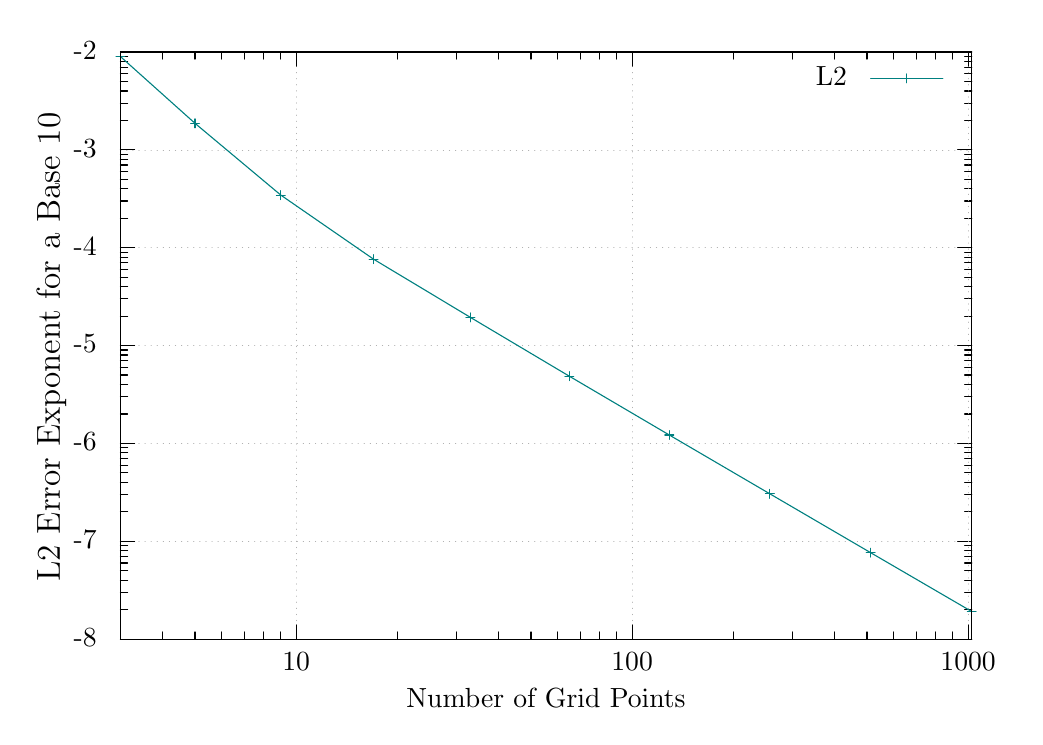
\begin{tikzpicture}[gnuplot]
%% generated with GNUPLOT 5.2p8 (Lua 5.3; terminal rev. Nov 2018, script rev. 108)
%% Tue 21 Sep 2021 05:01:33 PM EDT
\path (0.000,0.000) rectangle (12.500,8.750);
\gpcolor{color=gp lt color axes}
\gpsetlinetype{gp lt axes}
\gpsetdashtype{gp dt axes}
\gpsetlinewidth{0.50}
\draw[gp path] (1.136,0.985)--(11.947,0.985);
\gpcolor{color=gp lt color border}
\gpsetlinetype{gp lt border}
\gpsetdashtype{gp dt solid}
\gpsetlinewidth{1.00}
\draw[gp path] (1.136,0.985)--(1.316,0.985);
\draw[gp path] (11.947,0.985)--(11.767,0.985);
\node[gp node right] at (0.952,0.985) {{-8}};
\draw[gp path] (1.136,1.359)--(1.226,1.359);
\draw[gp path] (11.947,1.359)--(11.857,1.359);
\draw[gp path] (1.136,1.578)--(1.226,1.578);
\draw[gp path] (11.947,1.578)--(11.857,1.578);
\draw[gp path] (1.136,1.733)--(1.226,1.733);
\draw[gp path] (11.947,1.733)--(11.857,1.733);
\draw[gp path] (1.136,1.854)--(1.226,1.854);
\draw[gp path] (11.947,1.854)--(11.857,1.854);
\draw[gp path] (1.136,1.952)--(1.226,1.952);
\draw[gp path] (11.947,1.952)--(11.857,1.952);
\draw[gp path] (1.136,2.035)--(1.226,2.035);
\draw[gp path] (11.947,2.035)--(11.857,2.035);
\draw[gp path] (1.136,2.107)--(1.226,2.107);
\draw[gp path] (11.947,2.107)--(11.857,2.107);
\draw[gp path] (1.136,2.171)--(1.226,2.171);
\draw[gp path] (11.947,2.171)--(11.857,2.171);
\gpcolor{color=gp lt color axes}
\gpsetlinetype{gp lt axes}
\gpsetdashtype{gp dt axes}
\gpsetlinewidth{0.50}
\draw[gp path] (1.136,2.228)--(11.947,2.228);
\gpcolor{color=gp lt color border}
\gpsetlinetype{gp lt border}
\gpsetdashtype{gp dt solid}
\gpsetlinewidth{1.00}
\draw[gp path] (1.136,2.228)--(1.316,2.228);
\draw[gp path] (11.947,2.228)--(11.767,2.228);
\node[gp node right] at (0.952,2.228) {{-7}};
\draw[gp path] (1.136,2.602)--(1.226,2.602);
\draw[gp path] (11.947,2.602)--(11.857,2.602);
\draw[gp path] (1.136,2.821)--(1.226,2.821);
\draw[gp path] (11.947,2.821)--(11.857,2.821);
\draw[gp path] (1.136,2.976)--(1.226,2.976);
\draw[gp path] (11.947,2.976)--(11.857,2.976);
\draw[gp path] (1.136,3.096)--(1.226,3.096);
\draw[gp path] (11.947,3.096)--(11.857,3.096);
\draw[gp path] (1.136,3.195)--(1.226,3.195);
\draw[gp path] (11.947,3.195)--(11.857,3.195);
\draw[gp path] (1.136,3.278)--(1.226,3.278);
\draw[gp path] (11.947,3.278)--(11.857,3.278);
\draw[gp path] (1.136,3.350)--(1.226,3.350);
\draw[gp path] (11.947,3.350)--(11.857,3.350);
\draw[gp path] (1.136,3.413)--(1.226,3.413);
\draw[gp path] (11.947,3.413)--(11.857,3.413);
\gpcolor{color=gp lt color axes}
\gpsetlinetype{gp lt axes}
\gpsetdashtype{gp dt axes}
\gpsetlinewidth{0.50}
\draw[gp path] (1.136,3.470)--(11.947,3.470);
\gpcolor{color=gp lt color border}
\gpsetlinetype{gp lt border}
\gpsetdashtype{gp dt solid}
\gpsetlinewidth{1.00}
\draw[gp path] (1.136,3.470)--(1.316,3.470);
\draw[gp path] (11.947,3.470)--(11.767,3.470);
\node[gp node right] at (0.952,3.470) {{-6}};
\draw[gp path] (1.136,3.844)--(1.226,3.844);
\draw[gp path] (11.947,3.844)--(11.857,3.844);
\draw[gp path] (1.136,4.063)--(1.226,4.063);
\draw[gp path] (11.947,4.063)--(11.857,4.063);
\draw[gp path] (1.136,4.218)--(1.226,4.218);
\draw[gp path] (11.947,4.218)--(11.857,4.218);
\draw[gp path] (1.136,4.339)--(1.226,4.339);
\draw[gp path] (11.947,4.339)--(11.857,4.339);
\draw[gp path] (1.136,4.437)--(1.226,4.437);
\draw[gp path] (11.947,4.437)--(11.857,4.437);
\draw[gp path] (1.136,4.521)--(1.226,4.521);
\draw[gp path] (11.947,4.521)--(11.857,4.521);
\draw[gp path] (1.136,4.593)--(1.226,4.593);
\draw[gp path] (11.947,4.593)--(11.857,4.593);
\draw[gp path] (1.136,4.656)--(1.226,4.656);
\draw[gp path] (11.947,4.656)--(11.857,4.656);
\gpcolor{color=gp lt color axes}
\gpsetlinetype{gp lt axes}
\gpsetdashtype{gp dt axes}
\gpsetlinewidth{0.50}
\draw[gp path] (1.136,4.713)--(11.947,4.713);
\gpcolor{color=gp lt color border}
\gpsetlinetype{gp lt border}
\gpsetdashtype{gp dt solid}
\gpsetlinewidth{1.00}
\draw[gp path] (1.136,4.713)--(1.316,4.713);
\draw[gp path] (11.947,4.713)--(11.767,4.713);
\node[gp node right] at (0.952,4.713) {{-5}};
\draw[gp path] (1.136,5.087)--(1.226,5.087);
\draw[gp path] (11.947,5.087)--(11.857,5.087);
\draw[gp path] (1.136,5.306)--(1.226,5.306);
\draw[gp path] (11.947,5.306)--(11.857,5.306);
\draw[gp path] (1.136,5.461)--(1.226,5.461);
\draw[gp path] (11.947,5.461)--(11.857,5.461);
\draw[gp path] (1.136,5.582)--(1.226,5.582);
\draw[gp path] (11.947,5.582)--(11.857,5.582);
\draw[gp path] (1.136,5.680)--(1.226,5.680);
\draw[gp path] (11.947,5.680)--(11.857,5.680);
\draw[gp path] (1.136,5.763)--(1.226,5.763);
\draw[gp path] (11.947,5.763)--(11.857,5.763);
\draw[gp path] (1.136,5.835)--(1.226,5.835);
\draw[gp path] (11.947,5.835)--(11.857,5.835);
\draw[gp path] (1.136,5.899)--(1.226,5.899);
\draw[gp path] (11.947,5.899)--(11.857,5.899);
\gpcolor{color=gp lt color axes}
\gpsetlinetype{gp lt axes}
\gpsetdashtype{gp dt axes}
\gpsetlinewidth{0.50}
\draw[gp path] (1.136,5.956)--(11.947,5.956);
\gpcolor{color=gp lt color border}
\gpsetlinetype{gp lt border}
\gpsetdashtype{gp dt solid}
\gpsetlinewidth{1.00}
\draw[gp path] (1.136,5.956)--(1.316,5.956);
\draw[gp path] (11.947,5.956)--(11.767,5.956);
\node[gp node right] at (0.952,5.956) {{-4}};
\draw[gp path] (1.136,6.330)--(1.226,6.330);
\draw[gp path] (11.947,6.330)--(11.857,6.330);
\draw[gp path] (1.136,6.549)--(1.226,6.549);
\draw[gp path] (11.947,6.549)--(11.857,6.549);
\draw[gp path] (1.136,6.704)--(1.226,6.704);
\draw[gp path] (11.947,6.704)--(11.857,6.704);
\draw[gp path] (1.136,6.824)--(1.226,6.824);
\draw[gp path] (11.947,6.824)--(11.857,6.824);
\draw[gp path] (1.136,6.923)--(1.226,6.923);
\draw[gp path] (11.947,6.923)--(11.857,6.923);
\draw[gp path] (1.136,7.006)--(1.226,7.006);
\draw[gp path] (11.947,7.006)--(11.857,7.006);
\draw[gp path] (1.136,7.078)--(1.226,7.078);
\draw[gp path] (11.947,7.078)--(11.857,7.078);
\draw[gp path] (1.136,7.141)--(1.226,7.141);
\draw[gp path] (11.947,7.141)--(11.857,7.141);
\gpcolor{color=gp lt color axes}
\gpsetlinetype{gp lt axes}
\gpsetdashtype{gp dt axes}
\gpsetlinewidth{0.50}
\draw[gp path] (1.136,7.198)--(11.947,7.198);
\gpcolor{color=gp lt color border}
\gpsetlinetype{gp lt border}
\gpsetdashtype{gp dt solid}
\gpsetlinewidth{1.00}
\draw[gp path] (1.136,7.198)--(1.316,7.198);
\draw[gp path] (11.947,7.198)--(11.767,7.198);
\node[gp node right] at (0.952,7.198) {{-3}};
\draw[gp path] (1.136,7.572)--(1.226,7.572);
\draw[gp path] (11.947,7.572)--(11.857,7.572);
\draw[gp path] (1.136,7.791)--(1.226,7.791);
\draw[gp path] (11.947,7.791)--(11.857,7.791);
\draw[gp path] (1.136,7.946)--(1.226,7.946);
\draw[gp path] (11.947,7.946)--(11.857,7.946);
\draw[gp path] (1.136,8.067)--(1.226,8.067);
\draw[gp path] (11.947,8.067)--(11.857,8.067);
\draw[gp path] (1.136,8.165)--(1.226,8.165);
\draw[gp path] (11.947,8.165)--(11.857,8.165);
\draw[gp path] (1.136,8.249)--(1.226,8.249);
\draw[gp path] (11.947,8.249)--(11.857,8.249);
\draw[gp path] (1.136,8.321)--(1.226,8.321);
\draw[gp path] (11.947,8.321)--(11.857,8.321);
\draw[gp path] (1.136,8.384)--(1.226,8.384);
\draw[gp path] (11.947,8.384)--(11.857,8.384);
\gpcolor{color=gp lt color axes}
\gpsetlinetype{gp lt axes}
\gpsetdashtype{gp dt axes}
\gpsetlinewidth{0.50}
\draw[gp path] (1.136,8.441)--(11.947,8.441);
\gpcolor{color=gp lt color border}
\gpsetlinetype{gp lt border}
\gpsetdashtype{gp dt solid}
\gpsetlinewidth{1.00}
\draw[gp path] (1.136,8.441)--(1.316,8.441);
\draw[gp path] (11.947,8.441)--(11.767,8.441);
\node[gp node right] at (0.952,8.441) {{-2}};
\draw[gp path] (1.136,0.985)--(1.136,1.075);
\draw[gp path] (1.136,8.441)--(1.136,8.351);
\draw[gp path] (1.669,0.985)--(1.669,1.075);
\draw[gp path] (1.669,8.441)--(1.669,8.351);
\draw[gp path] (2.083,0.985)--(2.083,1.075);
\draw[gp path] (2.083,8.441)--(2.083,8.351);
\draw[gp path] (2.421,0.985)--(2.421,1.075);
\draw[gp path] (2.421,8.441)--(2.421,8.351);
\draw[gp path] (2.706,0.985)--(2.706,1.075);
\draw[gp path] (2.706,8.441)--(2.706,8.351);
\draw[gp path] (2.954,0.985)--(2.954,1.075);
\draw[gp path] (2.954,8.441)--(2.954,8.351);
\draw[gp path] (3.172,0.985)--(3.172,1.075);
\draw[gp path] (3.172,8.441)--(3.172,8.351);
\gpcolor{color=gp lt color axes}
\gpsetlinetype{gp lt axes}
\gpsetdashtype{gp dt axes}
\gpsetlinewidth{0.50}
\draw[gp path] (3.367,0.985)--(3.367,8.441);
\gpcolor{color=gp lt color border}
\gpsetlinetype{gp lt border}
\gpsetdashtype{gp dt solid}
\gpsetlinewidth{1.00}
\draw[gp path] (3.367,0.985)--(3.367,1.165);
\draw[gp path] (3.367,8.441)--(3.367,8.261);
\node[gp node center] at (3.367,0.677) {$10$};
\draw[gp path] (4.652,0.985)--(4.652,1.075);
\draw[gp path] (4.652,8.441)--(4.652,8.351);
\draw[gp path] (5.403,0.985)--(5.403,1.075);
\draw[gp path] (5.403,8.441)--(5.403,8.351);
\draw[gp path] (5.936,0.985)--(5.936,1.075);
\draw[gp path] (5.936,8.441)--(5.936,8.351);
\draw[gp path] (6.350,0.985)--(6.350,1.075);
\draw[gp path] (6.350,8.441)--(6.350,8.351);
\draw[gp path] (6.688,0.985)--(6.688,1.075);
\draw[gp path] (6.688,8.441)--(6.688,8.351);
\draw[gp path] (6.973,0.985)--(6.973,1.075);
\draw[gp path] (6.973,8.441)--(6.973,8.351);
\draw[gp path] (7.221,0.985)--(7.221,1.075);
\draw[gp path] (7.221,8.441)--(7.221,8.351);
\draw[gp path] (7.439,0.985)--(7.439,1.075);
\draw[gp path] (7.439,8.441)--(7.439,8.351);
\gpcolor{color=gp lt color axes}
\gpsetlinetype{gp lt axes}
\gpsetdashtype{gp dt axes}
\gpsetlinewidth{0.50}
\draw[gp path] (7.634,0.985)--(7.634,8.441);
\gpcolor{color=gp lt color border}
\gpsetlinetype{gp lt border}
\gpsetdashtype{gp dt solid}
\gpsetlinewidth{1.00}
\draw[gp path] (7.634,0.985)--(7.634,1.165);
\draw[gp path] (7.634,8.441)--(7.634,8.261);
\node[gp node center] at (7.634,0.677) {$100$};
\draw[gp path] (8.919,0.985)--(8.919,1.075);
\draw[gp path] (8.919,8.441)--(8.919,8.351);
\draw[gp path] (9.670,0.985)--(9.670,1.075);
\draw[gp path] (9.670,8.441)--(9.670,8.351);
\draw[gp path] (10.203,0.985)--(10.203,1.075);
\draw[gp path] (10.203,8.441)--(10.203,8.351);
\draw[gp path] (10.617,0.985)--(10.617,1.075);
\draw[gp path] (10.617,8.441)--(10.617,8.351);
\draw[gp path] (10.955,0.985)--(10.955,1.075);
\draw[gp path] (10.955,8.441)--(10.955,8.351);
\draw[gp path] (11.240,0.985)--(11.240,1.075);
\draw[gp path] (11.240,8.441)--(11.240,8.351);
\draw[gp path] (11.488,0.985)--(11.488,1.075);
\draw[gp path] (11.488,8.441)--(11.488,8.351);
\draw[gp path] (11.706,0.985)--(11.706,1.075);
\draw[gp path] (11.706,8.441)--(11.706,8.351);
\gpcolor{color=gp lt color axes}
\gpsetlinetype{gp lt axes}
\gpsetdashtype{gp dt axes}
\gpsetlinewidth{0.50}
\draw[gp path] (11.901,0.985)--(11.901,8.441);
\gpcolor{color=gp lt color border}
\gpsetlinetype{gp lt border}
\gpsetdashtype{gp dt solid}
\gpsetlinewidth{1.00}
\draw[gp path] (11.901,0.985)--(11.901,1.165);
\draw[gp path] (11.901,8.441)--(11.901,8.261);
\node[gp node center] at (11.901,0.677) {$1000$};
\draw[gp path] (1.136,8.441)--(1.136,0.985)--(11.947,0.985)--(11.947,8.441)--cycle;
\node[gp node center,rotate=-270,font={\fontsize{12.0pt}{14.4pt}\selectfont}] at (0.292,4.713) {L2 Error Exponent for a Base 10};
\node[gp node center] at (6.541,0.215) {Number of Grid Points};
\node[gp node right] at (10.479,8.107) {L2};
\gpcolor{rgb color={0.000,0.502,0.502}}
\draw[gp path] (10.663,8.107)--(11.579,8.107);
\draw[gp path] (1.136,8.383)--(2.083,7.535)--(3.172,6.624)--(4.350,5.810)--(5.580,5.071)%
  --(6.836,4.324)--(8.106,3.577)--(9.383,2.830)--(10.664,2.082)--(11.947,1.335);
\gpsetpointsize{4.00}
\gppoint{gp mark 1}{(1.136,8.383)}
\gppoint{gp mark 1}{(2.083,7.535)}
\gppoint{gp mark 1}{(3.172,6.624)}
\gppoint{gp mark 1}{(4.350,5.810)}
\gppoint{gp mark 1}{(5.580,5.071)}
\gppoint{gp mark 1}{(6.836,4.324)}
\gppoint{gp mark 1}{(8.106,3.577)}
\gppoint{gp mark 1}{(9.383,2.830)}
\gppoint{gp mark 1}{(10.664,2.082)}
\gppoint{gp mark 1}{(11.947,1.335)}
\gppoint{gp mark 1}{(11.121,8.107)}
\gpcolor{color=gp lt color border}
\draw[gp path] (1.136,8.441)--(1.136,0.985)--(11.947,0.985)--(11.947,8.441)--cycle;
%% coordinates of the plot area
\gpdefrectangularnode{gp plot 1}{\pgfpoint{1.136cm}{0.985cm}}{\pgfpoint{11.947cm}{8.441cm}}
\end{tikzpicture}
%% gnuplot variables

    \end{center}
\end{figure}





\begin{figure}
    \begin{center}
        \scalebox{0.75}{% This file was created with tikzplotlib v0.9.12.
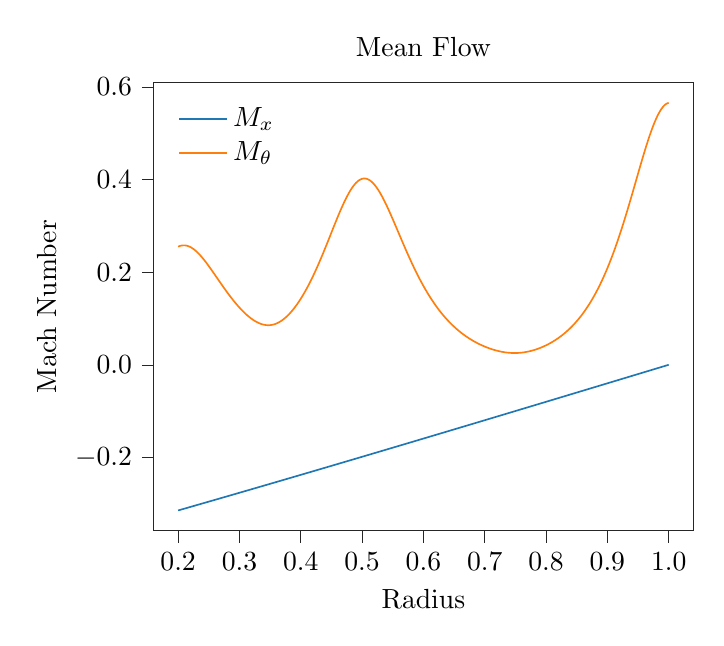
\begin{tikzpicture}

\definecolor{color0}{rgb}{0.12156862745098,0.466666666666667,0.705882352941177}
\definecolor{color1}{rgb}{1,0.498039215686275,0.0549019607843137}

\begin{axis}[
axis line style={white!15!black},
legend cell align={left},
legend style={
  fill opacity=0.8,
  draw opacity=1,
  text opacity=1,
  at={(0.03,0.97)},
  anchor=north west,
  draw=none
},
tick align=outside,
tick pos=left,
title={Mean Flow },
x grid style={white!80!black},
xlabel={Radius},
xmin=0.16, xmax=1.04,
xtick style={color=white!15!black},
xtick={0.1,0.2,0.3,0.4,0.5,0.6,0.7,0.8,0.9,1,1.1},
xticklabels={0.1,0.2,0.3,0.4,0.5,0.6,0.7,0.8,0.9,1.0,1.1},
y grid style={white!80!black},
ylabel={Mach Number},
ymin=-0.358579171685103, ymax=0.609698172253824,
ytick style={color=white!15!black},
ytick={-0.4,-0.2,0,0.2,0.4,0.6,0.8},
yticklabels={\ensuremath{-}0.4,\ensuremath{-}0.2,0.0,0.2,0.4,0.6,0.8}
]
\addplot [semithick, color0]
table {%
0.2 -0.314566565142425
0.2015625 -0.313973231598063
0.203125 -0.313379775407908
0.2046875 -0.312786196803778
0.20625 -0.31219249601754
0.2078125 -0.311598673281109
0.209375 -0.311004728826447
0.2109375 -0.310410662885563
0.2125 -0.309816475690513
0.2140625 -0.309222167473404
0.215625 -0.308627738466385
0.2171875 -0.308033188901657
0.21875 -0.307438519011464
0.2203125 -0.306843729028101
0.221875 -0.306248819183906
0.2234375 -0.305653789711266
0.225 -0.305058640842615
0.2265625 -0.304463372810433
0.228125 -0.303867985847246
0.2296875 -0.303272480185627
0.23125 -0.302676856058197
0.2328125 -0.302081113697619
0.234375 -0.301485253336607
0.2359375 -0.300889275207918
0.2375 -0.300293179544357
0.2390625 -0.299696966578772
0.240625 -0.29910063654406
0.2421875 -0.298504189673163
0.24375 -0.297907626199066
0.2453125 -0.297310946354804
0.246875 -0.296714150373453
0.2484375 -0.296117238488138
0.25 -0.295520210932026
0.2515625 -0.294923067938333
0.253125 -0.294325809740317
0.2546875 -0.293728436571281
0.25625 -0.293130948664575
0.2578125 -0.292533346253593
0.259375 -0.291935629571772
0.2609375 -0.291337798852597
0.2625 -0.290739854329594
0.2640625 -0.290141796236336
0.265625 -0.289543624806439
0.2671875 -0.288945340273564
0.26875 -0.288346942871416
0.2703125 -0.287748432833744
0.271875 -0.28714981039434
0.2734375 -0.286551075787042
0.275 -0.28595222924573
0.2765625 -0.285353271004329
0.278125 -0.284754201296807
0.2796875 -0.284155020357175
0.28125 -0.283555728419489
0.2828125 -0.282956325717846
0.284375 -0.282356812486389
0.2859375 -0.281757188959303
0.2875 -0.281157455370815
0.2890625 -0.280557611955196
0.290625 -0.27995765894676
0.2921875 -0.279357596579864
0.29375 -0.278757425088908
0.2953125 -0.278157144708332
0.296875 -0.277556755672622
0.2984375 -0.276956258216305
0.3 -0.27635565257395
0.3015625 -0.275754938980168
0.303125 -0.275154117669613
0.3046875 -0.274553188876981
0.30625 -0.273952152837011
0.3078125 -0.273351009784481
0.309375 -0.272749759954213
0.3109375 -0.27214840358107
0.3125 -0.271546940899957
0.3140625 -0.270945372145821
0.315625 -0.27034369755365
0.3171875 -0.269741917358471
0.31875 -0.269140031795357
0.3203125 -0.268538041099418
0.321875 -0.267935945505807
0.3234375 -0.267333745249717
0.325 -0.266731440566383
0.3265625 -0.266129031691081
0.328125 -0.265526518859126
0.3296875 -0.264923902305875
0.33125 -0.264321182266725
0.3328125 -0.263718358977114
0.334375 -0.263115432672518
0.3359375 -0.262512403588457
0.3375 -0.261909271960489
0.3390625 -0.261306038024212
0.340625 -0.260702702015264
0.3421875 -0.260099264169323
0.34375 -0.259495724722107
0.3453125 -0.258892083909374
0.346875 -0.258288341966921
0.3484375 -0.257684499130585
0.35 -0.257080555636242
0.3515625 -0.256476511719807
0.353125 -0.255872367617234
0.3546875 -0.255268123564519
0.35625 -0.254663779797693
0.3578125 -0.254059336552828
0.359375 -0.253454794066035
0.3609375 -0.252850152573463
0.3625 -0.252245412311301
0.3640625 -0.251640573515775
0.365625 -0.25103563642315
0.3671875 -0.25043060126973
0.36875 -0.249825468291857
0.3703125 -0.249220237725911
0.371875 -0.248614909808309
0.3734375 -0.248009484775508
0.375 -0.247403962864003
0.3765625 -0.246798344310325
0.378125 -0.246192629351044
0.3796875 -0.245586818222767
0.38125 -0.24498091116214
0.3828125 -0.244374908405845
0.384375 -0.243768810190601
0.3859375 -0.243162616753166
0.3875 -0.242556328330334
0.3890625 -0.241949945158937
0.390625 -0.241343467475843
0.3921875 -0.240736895517956
0.39375 -0.240130229522221
0.3953125 -0.239523469725615
0.396875 -0.238916616365153
0.3984375 -0.238309669677889
0.4 -0.23770262990091
0.4015625 -0.237095497271341
0.403125 -0.236488272026345
0.4046875 -0.235880954403117
0.40625 -0.235273544638891
0.4078125 -0.234666042970938
0.409375 -0.234058449636562
0.4109375 -0.233450764873104
0.4125 -0.232842988917941
0.4140625 -0.232235122008486
0.415625 -0.231627164382187
0.4171875 -0.231019116276527
0.41875 -0.230410977929025
0.4203125 -0.229802749577234
0.421875 -0.229194431458745
0.4234375 -0.228586023811182
0.425 -0.227977526872203
0.4265625 -0.227368940879503
0.428125 -0.226760266070811
0.4296875 -0.22615150268389
0.43125 -0.225542650956538
0.4328125 -0.224933711126589
0.434375 -0.224324683431909
0.4359375 -0.2237155681104
0.4375 -0.223106365399997
0.4390625 -0.222497075538671
0.440625 -0.221887698764424
0.4421875 -0.221278235315296
0.44375 -0.220668685429357
0.4453125 -0.220059049344713
0.446875 -0.219449327299504
0.4484375 -0.218839519531901
0.45 -0.21822962628011
0.4515625 -0.217619647782373
0.453125 -0.21700958427696
0.4546875 -0.21639943600218
0.45625 -0.215789203196369
0.4578125 -0.215178886097901
0.459375 -0.214568484945182
0.4609375 -0.213957999976648
0.4625 -0.21334743143077
0.4640625 -0.212736779546052
0.465625 -0.21212604456103
0.4671875 -0.211515226714272
0.46875 -0.210904326244379
0.4703125 -0.210293343389984
0.471875 -0.209682278389752
0.4734375 -0.209071131482379
0.475 -0.208459902906597
0.4765625 -0.207848592901165
0.478125 -0.207237201704876
0.4796875 -0.206625729556556
0.48125 -0.206014176695061
0.4828125 -0.205402543359278
0.484375 -0.204790829788126
0.4859375 -0.204179036220557
0.4875 -0.203567162895553
0.4890625 -0.202955210052125
0.490625 -0.202343177929319
0.4921875 -0.201731066766209
0.49375 -0.201118876801901
0.4953125 -0.200506608275533
0.496875 -0.19989426142627
0.4984375 -0.199281836493312
0.5 -0.198669333715887
0.5015625 -0.198056753333254
0.503125 -0.197444095584701
0.5046875 -0.196831360709549
0.50625 -0.196218548947147
0.5078125 -0.195605660536874
0.509375 -0.194992695718141
0.5109375 -0.194379654730386
0.5125 -0.193766537813078
0.5140625 -0.193153345205717
0.515625 -0.19254007714783
0.5171875 -0.191926733878976
0.51875 -0.191313315638742
0.5203125 -0.190699822666745
0.521875 -0.190086255202629
0.5234375 -0.18947261348607
0.525 -0.188858897756771
0.5265625 -0.188245108254466
0.528125 -0.187631245218915
0.5296875 -0.18701730888991
0.53125 -0.186403299507269
0.5328125 -0.185789217310838
0.534375 -0.185175062540495
0.5359375 -0.184560835436144
0.5375 -0.183946536237716
0.5390625 -0.183332165185173
0.540625 -0.182717722518503
0.5421875 -0.182103208477722
0.54375 -0.181488623302877
0.5453125 -0.180873967234038
0.546875 -0.180259240511305
0.5484375 -0.179644443374807
0.55 -0.179029576064698
0.5515625 -0.178414638821162
0.553125 -0.177799631884408
0.5546875 -0.177184555494672
0.55625 -0.17656940989222
0.5578125 -0.175954195317341
0.559375 -0.175338912010356
0.5609375 -0.174723560211609
0.5625 -0.17410814016147
0.5640625 -0.17349265210034
0.565625 -0.172877096268643
0.5671875 -0.17226147290683
0.56875 -0.17164578225538
0.5703125 -0.171030024554796
0.571875 -0.170414200045609
0.5734375 -0.169798308968375
0.575 -0.169182351563677
0.5765625 -0.168566328072123
0.578125 -0.167950238734347
0.5796875 -0.16733408379101
0.58125 -0.166717863482796
0.5828125 -0.166101578050417
0.584375 -0.165485227734609
0.5859375 -0.164868812776134
0.5875 -0.164252333415779
0.5890625 -0.163635789894357
0.590625 -0.163019182452705
0.5921875 -0.162402511331685
0.59375 -0.161785776772184
0.5953125 -0.161168979015113
0.596875 -0.160552118301411
0.5984375 -0.159935194872038
0.6 -0.159318208967979
0.6015625 -0.158701160830245
0.603125 -0.158084050699871
0.6046875 -0.157466878817914
0.60625 -0.156849645425458
0.6078125 -0.156232350763609
0.609375 -0.155614995073498
0.6109375 -0.154997578596281
0.6125 -0.154380101573134
0.6140625 -0.15376256424526
0.615625 -0.153144966853885
0.6171875 -0.152527309640257
0.61875 -0.151909592845649
0.6203125 -0.151291816711356
0.621875 -0.150673981478698
0.6234375 -0.150056087389016
0.625 -0.149438134683675
0.6265625 -0.148820123604062
0.628125 -0.14820205439159
0.6296875 -0.147583927287689
0.63125 -0.146965742533818
0.6328125 -0.146347500371453
0.634375 -0.145729201042096
0.6359375 -0.14511084478727
0.6375 -0.144492431848521
0.6390625 -0.143873962467415
0.640625 -0.143255436885543
0.6421875 -0.142636855344516
0.64375 -0.142018218085968
0.6453125 -0.141399525351553
0.646875 -0.140780777382949
0.6484375 -0.140161974421854
0.65 -0.139543116709988
0.6515625 -0.138924204489092
0.653125 -0.138305238000929
0.6546875 -0.137686217487282
0.65625 -0.137067143189957
0.6578125 -0.136448015350779
0.659375 -0.135828834211595
0.6609375 -0.135209600014273
0.6625 -0.134590313000702
0.6640625 -0.133970973412789
0.665625 -0.133351581492465
0.6671875 -0.13273213748168
0.66875 -0.132112641622403
0.6703125 -0.131493094156626
0.671875 -0.13087349532636
0.6734375 -0.130253845373634
0.675 -0.1296341445405
0.6765625 -0.129014393069028
0.678125 -0.12839459120131
0.6796875 -0.127774739179454
0.68125 -0.127154837245591
0.6828125 -0.12653488564187
0.684375 -0.125914884610459
0.6859375 -0.125294834393547
0.6875 -0.12467473523334
0.6890625 -0.124054587372064
0.690625 -0.123434391051966
0.6921875 -0.122814146515309
0.69375 -0.122193854004376
0.6953125 -0.121573513761469
0.696875 -0.120953126028908
0.6984375 -0.120332691049032
0.7 -0.1197122090642
0.7015625 -0.119091680316785
0.703125 -0.118471105049183
0.7046875 -0.117850483503806
0.70625 -0.117229815923084
0.7078125 -0.116609102549465
0.709375 -0.115988343625415
0.7109375 -0.115367539393419
0.7125 -0.114746690095978
0.7140625 -0.114125795975612
0.715625 -0.113504857274856
0.7171875 -0.112883874236266
0.71875 -0.112262847102412
0.7203125 -0.111641776115884
0.721875 -0.111020661519287
0.7234375 -0.110399503555244
0.725 -0.109778302466396
0.7265625 -0.109157058495398
0.728125 -0.108535771884924
0.7296875 -0.107914442877665
0.73125 -0.107293071716326
0.7328125 -0.106671658643631
0.734375 -0.10605020390232
0.7359375 -0.105428707735148
0.7375 -0.104807170384887
0.7390625 -0.104185592094326
0.740625 -0.103563973106267
0.7421875 -0.102942313663532
0.74375 -0.102320614008955
0.7453125 -0.101698874385389
0.746875 -0.1010770950357
0.7484375 -0.100455276202771
0.75 -0.0998334181294999
0.7515625 -0.0992115210587998
0.753125 -0.0985895852335994
0.7546875 -0.0979676108968424
0.75625 -0.0973455982914874
0.7578125 -0.0967235476605083
0.759375 -0.0961014592468934
0.7609375 -0.0954793332936462
0.7625 -0.0948571700437845
0.7640625 -0.0942349697403408
0.765625 -0.0936127326263622
0.7671875 -0.0929904589449099
0.76875 -0.0923681489390598
0.7703125 -0.0917458028519016
0.771875 -0.0911234209265392
0.7734375 -0.0905010034060907
0.775 -0.0898785505336877
0.7765625 -0.0892560625524761
0.778125 -0.0886335397056152
0.7796875 -0.0880109822362778
0.78125 -0.0873883903876507
0.7828125 -0.0867657644029336
0.784375 -0.0861431045253399
0.7859375 -0.0855204109980961
0.7875 -0.0848976840644419
0.7890625 -0.0842749239676299
0.790625 -0.0836521309509258
0.7921875 -0.0830293052576081
0.79375 -0.0824064471309682
0.7953125 -0.0817835568143099
0.796875 -0.0811606345509499
0.7984375 -0.0805376805842171
0.8 -0.0799146951574529
0.8015625 -0.079291678514011
0.803125 -0.0786686308972572
0.8046875 -0.0780455525505696
0.80625 -0.0774224437173381
0.8078125 -0.0767993046409646
0.809375 -0.0761761355648628
0.8109375 -0.0755529367324582
0.8125 -0.0749297083871877
0.8140625 -0.0743064507724999
0.815625 -0.0736831641318549
0.8171875 -0.073059848708724
0.81875 -0.0724365047465898
0.8203125 -0.071813132488946
0.821875 -0.0711897321792973
0.8234375 -0.0705663040611597
0.825 -0.0699428483780596
0.8265625 -0.0693193653735343
0.828125 -0.0686958552911321
0.8296875 -0.0680723183744114
0.83125 -0.0674487548669416
0.8328125 -0.0668251650123019
0.834375 -0.0662015490540821
0.8359375 -0.0655779072358824
0.8375 -0.0649542398013126
0.8390625 -0.0643305469939931
0.840625 -0.0637068290575537
0.8421875 -0.0630830862356343
0.84375 -0.0624593187718844
0.8453125 -0.0618355269099631
0.846875 -0.0612117108935392
0.8484375 -0.0605878709662909
0.85 -0.0599640073719054
0.8515625 -0.0593401203540797
0.853125 -0.0587162101565195
0.8546875 -0.0580922770229398
0.85625 -0.0574683211970645
0.8578125 -0.0568443429226261
0.859375 -0.0562203424433665
0.8609375 -0.0555963200030356
0.8625 -0.0549722758453923
0.8640625 -0.0543482102142038
0.865625 -0.0537241233532457
0.8671875 -0.0531000155063021
0.86875 -0.0524758869171648
0.8703125 -0.0518517378296344
0.871875 -0.0512275684875189
0.8734375 -0.0506033791346345
0.875 -0.0499791700148053
0.8765625 -0.0493549413718627
0.878125 -0.0487306934496463
0.8796875 -0.0481064264920028
0.88125 -0.0474821407427864
0.8828125 -0.0468578364458589
0.884375 -0.0462335138450891
0.8859375 -0.045609173184353
0.8875 -0.0449848147075337
0.8890625 -0.0443604386585211
0.890625 -0.0437360452812123
0.8921875 -0.0431116348195108
0.89375 -0.042487207517327
0.8953125 -0.0418627636185779
0.896875 -0.0412383033671867
0.8984375 -0.0406138270070833
0.9 -0.0399893347822038
0.9015625 -0.0393648269364904
0.903125 -0.0387403037138917
0.9046875 -0.0381157653583617
0.90625 -0.037491212113861
0.9078125 -0.0368666442243555
0.909375 -0.0362420619338172
0.9109375 -0.0356174654862236
0.9125 -0.0349928551255574
0.9140625 -0.0343682310958073
0.915625 -0.0337435936409669
0.9171875 -0.0331189430050354
0.91875 -0.0324942794320168
0.9203125 -0.0318696031659202
0.921875 -0.03124491445076
0.9234375 -0.0306202135305551
0.925 -0.0299955006493293
0.9265625 -0.0293707760511112
0.928125 -0.0287460399799336
0.9296875 -0.0281212926798342
0.93125 -0.0274965343948549
0.9328125 -0.0268717653690419
0.934375 -0.0262469858464456
0.9359375 -0.0256221960711204
0.9375 -0.024997396287125
0.9390625 -0.0243725867385215
0.940625 -0.0237477676693765
0.9421875 -0.0231229393237598
0.94375 -0.0224981019457448
0.9453125 -0.0218732557794089
0.946875 -0.0212484010688324
0.9484375 -0.0206235380580993
0.95 -0.0199986669912967
0.9515625 -0.0193737881125147
0.953125 -0.0187489016658469
0.9546875 -0.0181240078953893
0.95625 -0.0174991070452412
0.9578125 -0.0168741993595044
0.959375 -0.0162492850822834
0.9609375 -0.0156243644576856
0.9625 -0.0149994377298203
0.9640625 -0.0143745051427998
0.965625 -0.0137495669407382
0.9671875 -0.0131246233677519
0.96875 -0.0124996746679598
0.9703125 -0.0118747210854821
0.971875 -0.0112497628644416
0.9734375 -0.0106248002489625
0.975 -0.00999983348317079
0.9765625 -0.00937486281119418
0.978125 -0.00874988847716171
0.9796875 -0.00812491072520414
0.98125 -0.00749992979945334
0.9828125 -0.00687494594404237
0.984375 -0.00624995940310574
0.9859375 -0.00562497042077864
0.9875 -0.00499997924119756
0.9890625 -0.0043749861084996
0.990625 -0.00374999126682261
0.9921875 -0.00312499496030536
0.99375 -0.00249999743308688
0.9953125 -0.00187499892930699
0.996875 -0.00124999969310565
0.9984375 -0.000624999968623085
1 0
};
\addlegendentry{$M_{x}$}
\addplot [semithick, color1]
table {%
0.2 0.255065159843046
0.2015625 0.255968364411969
0.203125 0.256706833358219
0.2046875 0.257279572376127
0.20625 0.257686110072619
0.2078125 0.257926497257104
0.209375 0.258001302302394
0.2109375 0.257911602675627
0.2125 0.257658972790116
0.2140625 0.257245468377284
0.215625 0.256673607621338
0.2171875 0.255946349337276
0.21875 0.255067068504603
0.2203125 0.254039529494257
0.221875 0.25286785734447
0.2234375 0.251556507452602
0.225 0.250110234054432
0.2265625 0.248534057860345
0.228125 0.246833233209701
0.2296875 0.245013215091013
0.23125 0.243079626357068
0.2328125 0.241038225441498
0.234375 0.238894874857357
0.2359375 0.236655510729794
0.2375 0.234326113584628
0.2390625 0.231912680583411
0.240625 0.229421199363994
0.2421875 0.226857623614387
0.24375 0.224227850477382
0.2453125 0.221537699854474
0.246875 0.218792895650435
0.2484375 0.21599904897482
0.25 0.21316164329395
0.2515625 0.210286021506594
0.253125 0.207377374898871
0.2546875 0.204440733918698
0.25625 0.201480960697466
0.2578125 0.198502743236421
0.259375 0.19551059116732
0.2609375 0.192508832991191
0.2625 0.189501614695225
0.2640625 0.186492899645885
0.265625 0.183486469655856
0.2671875 0.180485927123467
0.26875 0.177494698145321
0.2703125 0.174516036506022
0.271875 0.171553028452757
0.2734375 0.168608598167034
0.275 0.165685513850817
0.2765625 0.162786394349561
0.278125 0.159913716240034
0.2796875 0.157069821316225
0.28125 0.154256924411978
0.2828125 0.151477121504055
0.284375 0.148732398044197
0.2859375 0.146024637473106
0.2875 0.143355629873271
0.2890625 0.140727080720902
0.290625 0.138140619700031
0.2921875 0.13559780954393
0.29375 0.133100154870287
0.2953125 0.130649110977115
0.296875 0.128246092566015
0.2984375 0.125892482358112
0.3 0.123589639565741
0.3015625 0.121338908179735
0.303125 0.119141625027891
0.3046875 0.116999127554962
0.30625 0.114912761268305
0.3078125 0.112883886786253
0.309375 0.110913886418458
0.3109375 0.109004170199123
0.3125 0.107156181285485
0.3140625 0.105371400625434
0.315625 0.103651350790409
0.3171875 0.1019975988631
0.31875 0.100411758264908
0.3203125 0.0988954894063168
0.321875 0.0974504990452432
0.3234375 0.0960785382451227
0.325 0.0947813988368702
0.3265625 0.0935609083079101
0.328125 0.0924189230679663
0.3296875 0.0913573200756757
0.33125 0.0903779868524443
0.3328125 0.089482809959776
0.334375 0.0886736620724435
0.3359375 0.0879523878403873
0.3375 0.0873207887944687
0.3390625 0.0867806076117272
0.340625 0.0863335121106115
0.3421875 0.085981079391489
0.34375 0.085724780568301
0.3453125 0.0855659665497199
0.346875 0.0855058553197153
0.3484375 0.0855455211364491
0.35 0.0856858860149973
0.3515625 0.0859277137854266
0.353125 0.0862716069268763
0.3546875 0.0867180062757169
0.35625 0.0872671935977731
0.3578125 0.0879192969077789
0.359375 0.0886742983202184
0.3609375 0.089532044130272
0.3625 0.0904922567562133
0.3640625 0.0915545481281322
0.365625 0.0927184340833403
0.3671875 0.0939833493256452
0.36875 0.0953486625217281
0.3703125 0.0968136911400023
0.371875 0.0983777156816692
0.3734375 0.100039993006174
0.375 0.101799768509913
0.3765625 0.103656286974313
0.378125 0.105608801954347
0.3796875 0.107656583628954
0.38125 0.109798925079123
0.3828125 0.112035146996802
0.384375 0.11436460085794
0.3859375 0.116786670616132
0.3875 0.1193007729899
0.3890625 0.121906356427498
0.390625 0.124602898838949
0.3921875 0.127389904186897
0.39375 0.130266898026433
0.3953125 0.133233422080402
0.396875 0.136289027931298
0.3984375 0.139433269904513
0.4 0.142665697210859
0.4015625 0.145985845409386
0.403125 0.149393227244884
0.4046875 0.152887322908421
0.40625 0.156467569763883
0.4078125 0.160133351579076
0.409375 0.163883987296415
0.4109375 0.167718719375798
0.4125 0.171636701740867
0.4140625 0.175636987359539
0.415625 0.179718515490483
0.4171875 0.183880098629044
0.41875 0.188120409189027
0.4203125 0.192437965960647
0.421875 0.196831120389881
0.4234375 0.201298042730311
0.425 0.205836708125276
0.4265625 0.210444882685797
0.428125 0.215120109638081
0.4296875 0.219859695623494
0.43125 0.224660697243575
0.4328125 0.229519907952808
0.434375 0.234433845412387
0.4359375 0.239398739428929
0.4375 0.244410520612798
0.4390625 0.249464809901279
0.440625 0.254556909101945
0.4421875 0.259681792621032
0.44375 0.264834100550136
0.4453125 0.27000813329177
0.446875 0.275197847909978
0.4484375 0.280396856395864
0.45 0.285598426039319
0.4515625 0.290795482096905
0.453125 0.295980612941552
0.4546875 0.301146077871998
0.45625 0.306283817748479
0.4578125 0.31138546860576
0.459375 0.316442378374904
0.4609375 0.32144562682116
0.4625 0.326386048776775
0.4640625 0.331254260714544
0.465625 0.336040690670567
0.4671875 0.340735611483277
0.46875 0.345329177270684
0.4703125 0.349811463019533
0.471875 0.35417250710938
0.4734375 0.358402356542188
0.475 0.362491114595036
0.4765625 0.366428990560886
0.478125 0.370206351191277
0.4796875 0.37381377340661
0.48125 0.377242097795612
0.4828125 0.380482482386889
0.484375 0.383526456143579
0.4859375 0.386365971608016
0.4875 0.388993456108193
0.4890625 0.391401860932495
0.490625 0.393584707884263
0.4921875 0.395536132643813
0.49375 0.397250924392459
0.4953125 0.398724561190988
0.496875 0.399953240653146
0.4984375 0.400933905512442
0.5 0.401664263746783
0.5015625 0.402142802998784
0.503125 0.402368799108529
0.5046875 0.402342318658297
0.50625 0.402064215513529
0.5078125 0.401536121429045
0.509375 0.400760430872516
0.5109375 0.399740280296358
0.5125 0.398479522163042
0.5140625 0.396982694095653
0.515625 0.395254983584066
0.5171875 0.39330218872638
0.51875 0.391130675524381
0.5203125 0.388747332280452
0.521875 0.386159521661241
0.5234375 0.383375031000781
0.525 0.380402021412906
0.5265625 0.37724897627048
0.528125 0.373924649587917
0.5296875 0.370438014814742
0.53125 0.366798214512707
0.5328125 0.363014511348306
0.534375 0.359096240787847
0.5359375 0.355052765834596
0.5375 0.350893434098191
0.5390625 0.346627537436659
0.540625 0.342264274361892
0.5421875 0.337812715351385
0.54375 0.333281771163073
0.5453125 0.328680164206925
0.546875 0.324016402987131
0.5484375 0.319298759592463
0.55 0.314535250180197
0.5515625 0.309733618370758
0.553125 0.304901321446166
0.5546875 0.300045519225358
0.55625 0.295173065473267
0.5578125 0.290290501688204
0.559375 0.285404053103047
0.5609375 0.280519626730042
0.5625 0.275642811276067
0.5640625 0.27077887875488
0.565625 0.265932787624734
0.5671875 0.261109187283532
0.56875 0.256312423759043
0.5703125 0.251546546438397
0.571875 0.246815315688742
0.5734375 0.242122211229442
0.575 0.237470441125182
0.5765625 0.232862951278719
0.578125 0.22830243531152
0.5796875 0.223791344730069
0.58125 0.219331899285021
0.5828125 0.21492609743956
0.584375 0.210575726872192
0.5859375 0.206282374947681
0.5875 0.202047439097858
0.5890625 0.197872137061639
0.590625 0.193757516940619
0.5921875 0.189704467033205
0.59375 0.185713725416266
0.5953125 0.181785889248833
0.596875 0.177921423777413
0.5984375 0.174120671027024
0.6 0.170383858166168
0.6015625 0.166711105537592
0.603125 0.163102434349923
0.6046875 0.159557774028135
0.60625 0.156076969223248
0.6078125 0.152659786483873
0.609375 0.149305920594004
0.6109375 0.146015000583079
0.6125 0.142786595415612
0.6140625 0.139620219368809
0.615625 0.136515337107451
0.6171875 0.13347136846603
0.61875 0.130487692948654
0.6203125 0.12756365395764
0.621875 0.124698562761982
0.6234375 0.121891702217005
0.625 0.119142330246641
0.6265625 0.116449683099675
0.628125 0.113812978391277
0.6296875 0.11123141794095
0.63125 0.108704190417859
0.6328125 0.106230473804262
0.634375 0.103809437687483
0.6359375 0.101440245390631
0.6375 0.0991220559518919
0.6390625 0.0968540259619605
0.640625 0.0946353112688321
0.6421875 0.092465068558833
0.64375 0.0903424568224584
0.6453125 0.088266638713247
0.646875 0.0862367818075993
0.6484375 0.0842520597731427
0.65 0.0823116534529223
0.6515625 0.0804147518724195
0.653125 0.0785605531761026
0.6546875 0.0767482654999489
0.65625 0.074977107786117
0.6578125 0.0732463105456957
0.659375 0.07155511657523
0.6609375 0.0699027816324986
0.6625 0.0682885750768002
0.6640625 0.0667117804788219
0.665625 0.0651716962049498
0.6671875 0.063667635980726
0.66875 0.0621989294379548
0.6703125 0.0607649226497941
0.671875 0.059364978658023
0.6734375 0.0579984779964363
0.675 0.0566648192142266
0.6765625 0.0553634194029264
0.678125 0.0540937147303553
0.6796875 0.0528551609847307
0.68125 0.0516472341318674
0.6828125 0.0504694308880978
0.684375 0.0493212693111629
0.6859375 0.0482022894109793
0.6875 0.0471120537816698
0.6890625 0.0460501482556922
0.690625 0.0450161825803071
0.6921875 0.0440097911157661
0.69375 0.043030633553821
0.6953125 0.0420783956540049
0.696875 0.0411527899940301
0.6984375 0.0402535567291964
0.7 0.0393804643541552
0.7015625 0.0385333104585603
0.703125 0.0377119224661578
0.7046875 0.0369161583445847
0.70625 0.03614590727077
0.7078125 0.0354010902341206
0.709375 0.0346816605569391
0.7109375 0.0339876043086025
0.7125 0.0333189405871274
0.7140625 0.032675721638941
0.715625 0.0320580327850901
0.7171875 0.0314659921199864
0.71875 0.030899749947283
0.7203125 0.0303594879168096
0.721875 0.0298454178271658
0.7234375 0.0293577800605058
0.725 0.028896841619993
0.7265625 0.02846289374629
0.728125 0.0280562490976937
0.7296875 0.0276772384892812
0.73125 0.0273262071995499
0.7328125 0.0270035108686346
0.734375 0.0267095110295417
0.7359375 0.0264445703327243
0.7375 0.0262090475435282
0.7390625 0.0260032924107508
0.740625 0.0258276405213213
0.7421875 0.0256824082697078
0.74375 0.025567888079597
0.7453125 0.0254843440186413
0.746875 0.02543200794361
0.7484375 0.0254110763027492
0.75 0.0254217077045359
0.7515625 0.0254640213381115
0.753125 0.0255380963015776
0.7546875 0.0256439718618399
0.75625 0.0257816486357861
0.7578125 0.0259510906494439
0.759375 0.0261522282015027
0.7609375 0.0263849614319338
0.7625 0.0266491644768043
0.7640625 0.0269446900775945
0.765625 0.0272713745074708
0.7671875 0.0276290426780044
0.76875 0.0280175132966183
0.7703125 0.0284366039568782
0.771875 0.0288861360590011
0.7734375 0.0293659394755854
0.775 0.0298758568960128
0.7765625 0.030415747801474
0.778125 0.0309854920398314
0.7796875 0.0315849929852943
0.78125 0.0322141802813672
0.7828125 0.0328730121767872
0.784375 0.0335614774730271
0.7859375 0.0342795971084747
0.7875 0.0350274254090058
0.7890625 0.0358050510372605
0.790625 0.0366125976742192
0.7921875 0.0374502244665543
0.79375 0.0383181262722576
0.7953125 0.0392165337353146
0.796875 0.040145713218003
0.7984375 0.0411059666168876
0.8 0.0420976310859398
0.8015625 0.0431210786874706
0.803125 0.0441767159889997
0.8046875 0.0452649836215835
0.80625 0.0463863558127949
0.8078125 0.0475413399053534
0.809375 0.0487304758704063
0.8109375 0.0499543358226658
0.8125 0.0512135235430355
0.8140625 0.0525086740128872
0.815625 0.0538404529629672
0.8171875 0.0552095564387755
0.81875 0.0566167103833332
0.8203125 0.0580626702374222
0.821875 0.0595482205566574
0.8234375 0.0610741746441408
0.825 0.062641374196886
0.8265625 0.0642506889637268
0.828125 0.0659030164120159
0.8296875 0.067599281400005
0.83125 0.0693404358514907
0.8328125 0.0711274584289652
0.834375 0.0729613542012303
0.8359375 0.07484315430113
0.8375 0.0767739155687956
0.8390625 0.0787547201755158
0.840625 0.0807866752230513
0.8421875 0.0828709123129645
0.84375 0.0850085870801981
0.8453125 0.0872008786848752
0.846875 0.0894489892559412
0.8484375 0.0917541432799597
0.85 0.0941175869280004
0.8515625 0.0965405873132023
0.853125 0.0990244316711992
0.8546875 0.101570426455177
0.85625 0.104179896336902
0.8578125 0.106854183104609
0.859375 0.109594644448144
0.8609375 0.112402652621281
0.8625 0.115279592970591
0.8640625 0.118226862319719
0.865625 0.121245867197353
0.8671875 0.124338021896614
0.86875 0.127504746353011
0.8703125 0.130747463827489
0.871875 0.134067598380528
0.8734375 0.13746657212265
0.875 0.14094580222606
0.8765625 0.144506697681637
0.878125 0.148150655784842
0.8796875 0.151879058333667
0.88125 0.15569326752118
0.8828125 0.159594621504825
0.884375 0.163584429634248
0.8859375 0.167663967319096
0.8875 0.171834470518073
0.8890625 0.176097129830408
0.890625 0.180453084170948
0.8921875 0.184903414010309
0.89375 0.189449134161866
0.8953125 0.194091186097979
0.896875 0.198830429778696
0.8984375 0.203667634977241
0.9 0.208603472088054
0.9015625 0.213638502404859
0.903125 0.218773167858416
0.9046875 0.22400778020613
0.90625 0.229342509668755
0.9078125 0.234777373012944
0.909375 0.24031222108247
0.9109375 0.245946725785683
0.9125 0.251680366552035
0.9140625 0.25751241627655
0.915625 0.263441926777863
0.9171875 0.269467713802905
0.91875 0.275588341619623
0.9203125 0.281802107248194
0.921875 0.288107024391076
0.9234375 0.294500807132996
0.925 0.300980853493419
0.9265625 0.307544228926396
0.928125 0.314187649875617
0.9296875 0.320907467506142
0.93125 0.327699651748462
0.9328125 0.334559775805034
0.934375 0.341483001284309
0.9359375 0.348464064142019
0.9375 0.355497261624187
0.9390625 0.36257644042046
0.940625 0.369694986249733
0.9421875 0.376845815112347
0.94375 0.384021366453792
0.9453125 0.391213598493737
0.946875 0.398413985980555
0.9484375 0.405613520635077
0.95 0.412802714547513
0.9515625 0.419971606787799
0.953125 0.427109773481643
0.9546875 0.434206341591764
0.95625 0.44125000662576
0.9578125 0.448229054468482
0.959375 0.455131387507252
0.9609375 0.461944555182711
0.9625 0.468655789056426
0.9640625 0.475252042438538
0.965625 0.481720034565212
0.9671875 0.488046299256582
0.96875 0.494217237922058
0.9703125 0.500219176712006
0.971875 0.506038427543904
0.9734375 0.511661352658388
0.975 0.517074432287396
0.9765625 0.522264334944558
0.978125 0.527217989778637
0.9796875 0.531922660365945
0.98125 0.536366019259179
0.9828125 0.540536222559617
0.984375 0.544421983739021
0.9859375 0.548012645908313
0.9875 0.55129825171366
0.9890625 0.554269610038046
0.990625 0.556918358698616
0.9921875 0.559237022357485
0.99375 0.561219064906353
0.9953125 0.562858935642828
0.996875 0.564152108628062
0.9984375 0.565095114699835
1 0.565685565711145
};
\addlegendentry{$M_{\theta}$}
\end{axis}

\end{tikzpicture}
}
    \end{center}
\end{figure}


\begin{figure}
    \begin{center}
        \scalebox{0.75}{% This file was created with tikzplotlib v0.9.12.
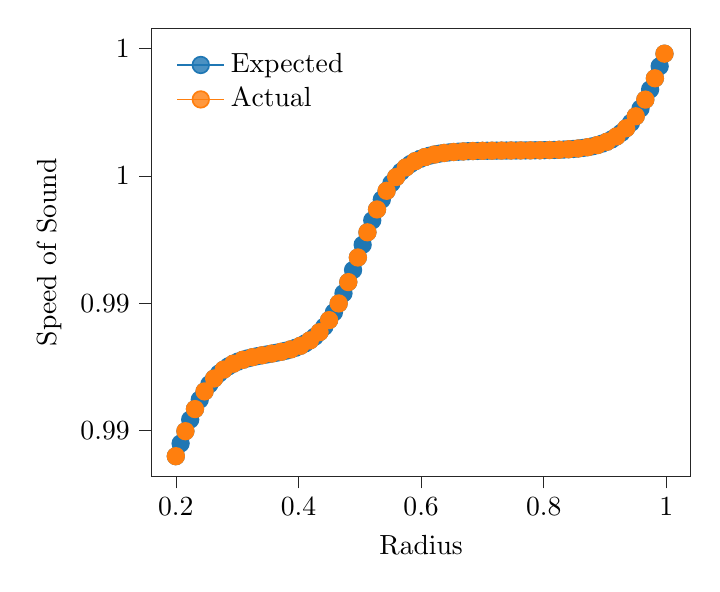
\begin{tikzpicture}

\definecolor{color0}{rgb}{0.12156862745098,0.466666666666667,0.705882352941177}
\definecolor{color1}{rgb}{1,0.498039215686275,0.0549019607843137}

\begin{axis}[
axis line style={white!15!black},
legend cell align={left},
legend style={
  fill opacity=0.8,
  draw opacity=1,
  text opacity=1,
  at={(0.03,0.97)},
  anchor=north west,
  draw=none
},
tick align=outside,
tick pos=left,
x grid style={white!80!black},
xlabel={Radius},
xmin=0.16, xmax=1.04,
xtick style={color=white!15!black},
y grid style={white!80!black},
ylabel={Speed of Sound},
ymin=0.98320056903035, ymax=1.00079997290332,
ytick style={color=white!15!black}
]
\addplot [semithick, color0, mark=*, mark size=3, mark repeat=5, mark options={solid}]
table {%
0.2 0.984000541933667
0.2015625 0.984100548886647
0.203125 0.984200432419622
0.2046875 0.984300068384446
0.20625 0.984399333875707
0.2078125 0.984498107834061
0.209375 0.984596271630271
0.2109375 0.984693709624082
0.2125 0.984790309692462
0.2140625 0.984885963722324
0.215625 0.984980568063398
0.2171875 0.985074023937652
0.21875 0.985166237802302
0.2203125 0.985257121664242
0.221875 0.985346593344428
0.2234375 0.985434576691501
0.225 0.985521001744648
0.2265625 0.985605804846342
0.228125 0.985688928706271
0.2296875 0.985770322418282
0.23125 0.985849941432696
0.2328125 0.985927747486754
0.234375 0.986003708496322
0.2359375 0.986077798412233
0.2375 0.986149997044859
0.2390625 0.986220289860638
0.240625 0.986288667754308
0.2421875 0.986355126800626
0.24375 0.986419667989276
0.2453125 0.986482296946548
0.246875 0.986543023647233
0.2484375 0.986601862119971
0.25 0.986658830149088
0.2515625 0.986713948975696
0.253125 0.98676724300061
0.2546875 0.98681873949133
0.25625 0.986868468295113
0.2578125 0.986916461559873
0.259375 0.986962753464396
0.2609375 0.987007379959106
0.2625 0.987050378518398
0.2640625 0.987091787905317
0.265625 0.987131647949157
0.2671875 0.987169999336396
0.26875 0.98720688341517
0.2703125 0.987242342013376
0.271875 0.987276417270339
0.2734375 0.987309151481869
0.275 0.987340586958444
0.2765625 0.987370765896143
0.278125 0.987399730259926
0.2796875 0.987427521678759
0.28125 0.987454181352077
0.2828125 0.987479749967015
0.284375 0.987504267625839
0.2859375 0.987527773782981
0.2875 0.987550307191088
0.2890625 0.987571905855486
0.290625 0.987592606996474
0.2921875 0.987612447018872
0.29375 0.987631461488276
0.2953125 0.987649685113462
0.296875 0.987667151734442
0.2984375 0.987683894315661
0.3 0.987699944943884
0.3015625 0.987715334830319
0.303125 0.987730094316565
0.3046875 0.987744252883996
0.30625 0.987757839166223
0.3078125 0.987770880964282
0.309375 0.987783405264264
0.3109375 0.987795438257075
0.3125 0.987807005360076
0.3140625 0.987818131240364
0.315625 0.987828839839472
0.3171875 0.987839154399291
0.31875 0.98784909748904
0.3203125 0.987858691033117
0.321875 0.9878679563397
0.3234375 0.987876914129958
0.325 0.987885584567766
0.3265625 0.987893987289837
0.328125 0.98790214143616
0.3296875 0.987910065680699
0.33125 0.987917778262275
0.3328125 0.987925297015572
0.334375 0.987932639402246
0.3359375 0.987939822542074
0.3375 0.987946863244137
0.3390625 0.987953778037998
0.340625 0.987960583204877
0.3421875 0.987967294808789
0.34375 0.98797392872766
0.3453125 0.987980500684408
0.346875 0.987987026277992
0.3484375 0.987993521014427
0.35 0.988000000337782
0.3515625 0.988006479661155
0.353125 0.988012974397646
0.3546875 0.988019499991323
0.35625 0.988026071948201
0.3578125 0.988032705867241
0.359375 0.988039417471358
0.3609375 0.988046222638482
0.3625 0.988053137432628
0.3640625 0.988060178135015
0.365625 0.988067361275209
0.3671875 0.98807470366229
0.36875 0.988082222416037
0.3703125 0.988089934998106
0.371875 0.988097859243185
0.3734375 0.988106013390094
0.375 0.988114416112798
0.3765625 0.988123086551289
0.378125 0.988132044342281
0.3796875 0.988141309649652
0.38125 0.988150903194572
0.3828125 0.98816084628522
0.384375 0.988171160845998
0.3859375 0.988181869446127
0.3875 0.9881929953275
0.3890625 0.988204562431654
0.390625 0.988216595425687
0.3921875 0.988229119726965
0.39375 0.988242161526395
0.3953125 0.988255747810073
0.396875 0.988269906379039
0.3984375 0.988284665866907
0.4 0.988300055755055
0.4015625 0.988316106385087
0.403125 0.988332848968214
0.4046875 0.988350315591207
0.40625 0.988368539218517
0.4078125 0.988387553690159
0.409375 0.988407393714916
0.4109375 0.988428094858389
0.4125 0.988449693525406
0.4140625 0.988472226936272
0.415625 0.988495733096318
0.4171875 0.988520250758199
0.41875 0.988545819376356
0.4203125 0.988572479053063
0.421875 0.988600270475462
0.4234375 0.988629234842998
0.425 0.988659413784646
0.4265625 0.988690849265375
0.428125 0.988723583481276
0.4296875 0.988757658742837
0.43125 0.98879311734588
0.4328125 0.988830001429742
0.434375 0.988868352822332
0.4359375 0.9889082128718
0.4375 0.988949622264638
0.4390625 0.988992620830155
0.440625 0.989037247331411
0.4421875 0.989083539242818
0.44375 0.989131532514817
0.4453125 0.989181261326212
0.446875 0.989232757824935
0.4484375 0.989286051858266
0.45 0.989341170693724
0.4515625 0.989398138732145
0.453125 0.989456977214666
0.4546875 0.989517703925637
0.45625 0.989580332893724
0.4578125 0.989644874093744
0.459375 0.989711333152017
0.4609375 0.989779711058255
0.4625 0.989850003887249
0.4640625 0.989922202533768
0.465625 0.989996292464284
0.4671875 0.990072253489208
0.46875 0.99015005955941
0.4703125 0.990229678590797
0.471875 0.990311072320652
0.4734375 0.99039419619934
0.475 0.990478999320756
0.4765625 0.990565424394636
0.478125 0.990653407763507
0.4796875 0.990742879466609
0.48125 0.99083376335264
0.4828125 0.990925977242617
0.484375 0.991019433143496
0.4859375 0.991114037512562
0.4875 0.991209691571851
0.4890625 0.991306291671168
0.490625 0.991403729697502
0.4921875 0.991501893527903
0.49375 0.991600667522201
0.4953125 0.99169993305125
0.496875 0.991799569055799
0.4984375 0.991899452630537
0.5 0.991999459627421
0.5015625 0.992099465272067
0.503125 0.99219934478671
0.5046875 0.992298974013166
0.50625 0.992398230029186
0.5078125 0.992496991751752
0.509375 0.992595140521059
0.5109375 0.992692560659307
0.5125 0.992789139998857
0.5140625 0.99288477037483
0.515625 0.992979348077864
0.5171875 0.99307277426338
0.51875 0.993164955314424
0.5203125 0.993255803155917
0.521875 0.993345235518834
0.5234375 0.993433176153603
0.525 0.993519554992716
0.5265625 0.993604308263212
0.528125 0.993687378550314
0.5296875 0.993768714814062
0.53125 0.993848272361297
0.5328125 0.993926012775751
0.534375 0.994001903809366
0.5359375 0.99407591923823
0.5375 0.994148038686721
0.5390625 0.99421824742356
0.540625 0.994286536133559
0.5421875 0.994352900668823
0.54375 0.994417341783093
0.5453125 0.994479864852854
0.546875 0.994540479588594
0.5484375 0.994599199739509
0.55 0.994656042794637
0.5515625 0.994711029683234
0.553125 0.994764184476907
0.5546875 0.994815534095789
0.55625 0.994865108020749
0.5578125 0.99491293801338
0.559375 0.99495905784526
0.5609375 0.995003503037712
0.5625 0.995046310613072
0.5640625 0.995087518858254
0.565625 0.995127167101171
0.5671875 0.995165295500434
0.56875 0.99520194484852
0.5703125 0.995237156388507
0.571875 0.995270971644298
0.5734375 0.995303432264168
0.575 0.995334579877347
0.5765625 0.995364455963282
0.578125 0.995393101733155
0.5796875 0.995420558023162
0.58125 0.995446865199025
0.5828125 0.995472063071189
0.584375 0.9954961908201
0.5859375 0.995519286930997
0.5875 0.995541389137587
0.5890625 0.995562534374025
0.590625 0.995582758734604
0.5921875 0.995602097440566
0.59375 0.995620584813474
0.5953125 0.995638254254612
0.596875 0.995655138229866
0.5984375 0.995671268259608
0.6 0.995686674913096
0.6015625 0.995701387806942
0.603125 0.995715435607232
0.6046875 0.995728846034892
0.60625 0.99574164587393
0.6078125 0.995753860982223
0.609375 0.995765516304507
0.6109375 0.995776635887292
0.6125 0.995787242895424
0.6140625 0.995797359630043
0.615625 0.995807007547711
0.6171875 0.995816207280501
0.61875 0.995824978656858
0.6203125 0.995833340723064
0.621875 0.995841311765143
0.6234375 0.995848909331092
0.625 0.995856150253272
0.6265625 0.995863050670899
0.628125 0.995869626052497
0.6296875 0.99587589121825
0.63125 0.995881860362164
0.6328125 0.995887547073985
0.634375 0.995892964360806
0.6359375 0.995898124668321
0.6375 0.995903039901678
0.6390625 0.995907721445908
0.640625 0.995912180185882
0.6421875 0.995916426525794
0.64375 0.995920470408134
0.6453125 0.995924321332153
0.646875 0.995927988371789
0.6484375 0.995931480193072
0.65 0.995934805070983
0.6515625 0.995937970905779
0.653125 0.99594098523878
0.6546875 0.995943855267619
0.65625 0.995946587860976
0.6578125 0.995949189572774
0.659375 0.995951666655872
0.6609375 0.995954025075258
0.6625 0.99595627052074
0.6640625 0.995958408419154
0.665625 0.995960443946116
0.6671875 0.995962382037296
0.66875 0.995964227399259
0.6703125 0.995965984519872
0.671875 0.995967657678284
0.6734375 0.995969250954509
0.675 0.995970768238611
0.6765625 0.995972213239507
0.678125 0.995973589493407
0.6796875 0.995974900371901
0.68125 0.995976149089699
0.6828125 0.995977338712054
0.684375 0.995978472161855
0.6859375 0.995979552226434
0.6875 0.995980581564065
0.6890625 0.995981562710198
0.690625 0.995982498083416
0.6921875 0.995983389991139
0.69375 0.995984240635083
0.6953125 0.995985052116483
0.696875 0.995985826441091
0.6984375 0.99598656552396
0.7 0.995987271194022
0.7015625 0.995987945198473
0.703125 0.995988589206969
0.7046875 0.995989204815643
0.70625 0.995989793550959
0.7078125 0.995990356873398
0.709375 0.995990896180996
0.7109375 0.99599141281273
0.7125 0.99599190805178
0.7140625 0.99599238312864
0.715625 0.995992839224128
0.7171875 0.995993277472259
0.71875 0.995993698963021
0.7203125 0.99599410474504
0.721875 0.99599449582815
0.7234375 0.995994873185871
0.725 0.995995237757798
0.7265625 0.995995590451909
0.728125 0.995995932146805
0.7296875 0.995996263693868
0.73125 0.995996585919359
0.7328125 0.995996899626465
0.734375 0.995997205597271
0.7359375 0.9959975045947
0.7375 0.995997797364393
0.7390625 0.995998084636562
0.740625 0.995998367127788
0.7421875 0.995998645542801
0.74375 0.995998920576223
0.7453125 0.995999192914293
0.746875 0.995999463236562
0.7484375 0.995999732217585
0.75 0.996000000528589
0.7515625 0.996000268839138
0.753125 0.996000537818796
0.7546875 0.996000808138787
0.75625 0.996001080473659
0.7578125 0.996001355502957
0.759375 0.996001633912908
0.7609375 0.996001916398121
0.7625 0.996002203663312
0.7640625 0.996002496425045
0.765625 0.996002795413511
0.7671875 0.996003101374329
0.76875 0.996003415070396
0.7703125 0.996003737283773
0.771875 0.996004068817611
0.7734375 0.996004410498143
0.775 0.996004763176713
0.7765625 0.996005127731883
0.778125 0.996005505071589
0.7796875 0.996005896135382
0.78125 0.996006301896732
0.7828125 0.996006723365422
0.784375 0.996007161590024
0.7859375 0.996007617660467
0.7875 0.996008092710702
0.7890625 0.996008587921481
0.790625 0.996009104523228
0.7921875 0.996009643799046
0.79375 0.996010207087836
0.7953125 0.996010795787547
0.796875 0.996011411358571
0.7984375 0.996012055327279
0.8 0.996012729289704
0.8015625 0.996013434915398
0.803125 0.996014173951444
0.8046875 0.996014948226658
0.80625 0.99601575965597
0.8078125 0.996016610245002
0.809375 0.99601750209485
0.8109375 0.996018437407087
0.8125 0.996019418488979
0.8140625 0.99602044775895
0.815625 0.996021527752279
0.8171875 0.996022661127064
0.81875 0.996023850670446
0.8203125 0.996025099305121
0.821875 0.99602641009613
0.8234375 0.996027786257968
0.825 0.996029231161992
0.8265625 0.996030748344171
0.828125 0.996032341513167
0.8296875 0.996034014558775
0.83125 0.996035771560727
0.8328125 0.996037616797878
0.834375 0.996039554757779
0.8359375 0.996041590146669
0.8375 0.996043727899874
0.8390625 0.996045973192643
0.840625 0.996048331451433
0.8421875 0.996050808365651
0.84375 0.99605340989986
0.8453125 0.996056142306476
0.846875 0.996059012138958
0.8484375 0.99606202626549
0.85 0.996065191883192
0.8515625 0.996068516532841
0.853125 0.996072008114122
0.8546875 0.996075674901416
0.85625 0.996079525560123
0.8578125 0.996083569163517
0.859375 0.996087815210152
0.8609375 0.996092273641784
0.8625 0.996096954861836
0.8640625 0.996101869754369
0.865625 0.996107029703561
0.8671875 0.996112446613664
0.86875 0.99611813292943
0.8703125 0.996124101656964
0.871875 0.996130366384967
0.8734375 0.996136941306354
0.875 0.996143841240155
0.8765625 0.996151081653687
0.878125 0.996158678684891
0.8796875 0.996166649164795
0.88125 0.996175010639986
0.8828125 0.996183781395013
0.884375 0.996192980474604
0.8859375 0.99620262770557
0.8875 0.996212743718267
0.8890625 0.996223349967452
0.890625 0.996234468752366
0.8921875 0.996246123235863
0.89375 0.996258337462352
0.8953125 0.996271136374368
0.896875 0.996284545827466
0.8984375 0.99629859260322
0.9 0.996313304419992
0.9015625 0.996328709941177
0.903125 0.996344838780554
0.9046875 0.996361721504406
0.90625 0.996379389629974
0.9078125 0.996397875619856
0.909375 0.996417212871876
0.9109375 0.996437435703965
0.9125 0.99645857933354
0.9140625 0.996480679850876
0.915625 0.996503774185906
0.9171875 0.996527900067896
0.91875 0.996553095977414
0.9203125 0.996579401090003
0.921875 0.996606855210946
0.9234375 0.996635498700543
0.925 0.996665372389287
0.9265625 0.996696517482366
0.928125 0.996728975452927
0.9296875 0.996762787923574
0.93125 0.996797996535619
0.9328125 0.996834642805644
0.934375 0.99687276796903
0.9359375 0.996912412810164
0.9375 0.996953617479149
0.9390625 0.996996421294959
0.940625 0.997040862535105
0.9421875 0.997086978212043
0.94375 0.997134803836707
0.9453125 0.997184373169752
0.946875 0.997235717961291
0.9484375 0.997288867680121
0.95 0.997343849233688
0.9515625 0.99740068668026
0.953125 0.997459400935069
0.9546875 0.997520009472411
0.95625 0.997582526025983
0.9578125 0.997646960289984
0.959375 0.997713317623768
0.9609375 0.997781598763074
0.9625 0.997851799541075
0.9640625 0.997923910622686
0.965625 0.99799791725571
0.9671875 0.998073799042532
0.96875 0.998151529736121
0.9703125 0.998231077064117
0.971875 0.998312402584702
0.9734375 0.998395461577857
0.975 0.998480202975387
0.9765625 0.998566569332831
0.978125 0.998654496846022
0.9796875 0.998743915414651
0.98125 0.998834748754659
0.9828125 0.998926914560766
0.984375 0.999020324719782
0.9859375 0.99911488557469
0.9875 0.99921049823879
0.9890625 0.999307058958444
0.990625 0.999404459522227
0.9921875 0.999502587713568
0.99375 0.999601327803226
0.9953125 0.999700561077321
0.996875 0.999800166395987
0.9984375 0.999900020777216
1 1
};
\addlegendentry{Expected}
\addplot [semithick, color1, mark=*, mark size=3, mark repeat=10, mark options={solid}]
table {%
0.2 0.984000542019354
0.2015625 0.984100538570465
0.203125 0.984200411755927
0.2046875 0.984300037478986
0.20625 0.984399292884513
0.2078125 0.984498056961819
0.209375 0.984596211128208
0.2109375 0.98469363978739
0.2125 0.984790230857325
0.2140625 0.984885876262573
0.215625 0.98498047238688
0.2171875 0.985073920482345
0.21875 0.985166127032258
0.2203125 0.985257004065404
0.221875 0.985346469420391
0.2234375 0.985434446959279
0.225 0.98552086673049
0.2265625 0.985605665081666
0.228125 0.985688784723747
0.2296875 0.985770174748117
0.23125 0.985849790599148
0.2328125 0.985927594004909
0.234375 0.986003552869154
0.2359375 0.986077641127965
0.2375 0.986149838574637
0.2390625 0.986220130656513
0.240625 0.986288508247539
0.2421875 0.986354967400289
0.24375 0.986419509081172
0.2453125 0.986482138892399
0.246875 0.986542866784147
0.2484375 0.98660170676016
0.25 0.986658676579815
0.2515625 0.986713797459438
0.253125 0.986767093775402
0.2546875 0.986818592771284
0.25625 0.986868324271075
0.2578125 0.98691632040021
0.259375 0.986962615315875
0.2609375 0.987007244947868
0.2625 0.987050246750991
0.2640625 0.987091659469774
0.265625 0.987131522916112
0.2671875 0.987169877760217
0.26875 0.987206765335094
0.2703125 0.987242227454642
0.271875 0.987276306245304
0.2734375 0.987309043991106
0.275 0.987340482991801
0.2765625 0.987370665433774
0.278125 0.987399633273278
0.2796875 0.987427428131517
0.28125 0.987454091201058
0.2828125 0.987479663163019
0.284375 0.987504184114449
0.2859375 0.987527693505313
0.2875 0.98755023008449
0.2890625 0.987571831854191
0.290625 0.9875925360322
0.2921875 0.987612379021383
0.29375 0.987631396385893
0.2953125 0.987649622833532
0.296875 0.987667092203763
0.2984375 0.987683837460875
0.3 0.987699890691827
0.3015625 0.987715283108339
0.303125 0.987730045052807
0.3046875 0.987744206007658
0.30625 0.987757794607782
0.3078125 0.987770838655695
0.309375 0.987783365139148
0.3109375 0.98779540025086
0.3125 0.987806969410141
0.3140625 0.987818097286156
0.315625 0.987828807822605
0.3171875 0.987839124263634
0.31875 0.98784906918079
0.3203125 0.987858664500862
0.321875 0.987867931534466
0.3234375 0.987876891005252
0.325 0.987885563079613
0.3265625 0.987893967396799
0.328125 0.987902123099364
0.3296875 0.987910048863849
0.33125 0.987917762931659
0.3328125 0.987925283140076
0.334375 0.987932626953352
0.3359375 0.987939811493866
0.3375 0.987946853573297
0.3390625 0.987953769723811
0.340625 0.98796057622922
0.3421875 0.987967289156136
0.34375 0.987973924385075
0.3453125 0.987980497641544
0.346875 0.987987024527085
0.3484375 0.987993520550299
0.35 0.988000001157834
0.3515625 0.988006481765371
0.353125 0.98801297778859
0.3546875 0.988019504674139
0.35625 0.988026077930618
0.3578125 0.988032713159569
0.359375 0.988039426086497
0.3609375 0.988046232591919
0.3625 0.988053148742442
0.3640625 0.98806019082188
0.365625 0.988067375362393
0.3671875 0.988074719175661
0.36875 0.988082239384058
0.3703125 0.988089953451836
0.371875 0.988097879216269
0.3734375 0.988106034918762
0.375 0.988114439235851
0.3765625 0.988123111310083
0.378125 0.988132070780705
0.3796875 0.988141337814104
0.38125 0.988150933133922
0.3828125 0.988160878050769
0.384375 0.988171194491426
0.3859375 0.988181905027431
0.3875 0.988193032902921
0.3890625 0.988204602061585
0.390625 0.988216637172577
0.3921875 0.988229163655196
0.39375 0.988242207702146
0.3953125 0.988255796301162
0.396875 0.988269957254748
0.3984375 0.988284719197773
0.4 0.988300111612648
0.4015625 0.988316164841748
0.403125 0.98833291009677
0.4046875 0.988350379464653
0.40625 0.988368605909658
0.4078125 0.988387623271224
0.409375 0.988407466257124
0.4109375 0.988428170431479
0.4125 0.988449772197124
0.4140625 0.988472308771811
0.415625 0.988495818157714
0.4171875 0.988520339103674
0.41875 0.988545911059617
0.4203125 0.988572574122552
0.421875 0.988600368973554
0.4234375 0.988629336805148
0.425 0.988659519238492
0.4265625 0.988690958229793
0.428125 0.988723695965391
0.4296875 0.988757774744993
0.43125 0.988793236852577
0.4328125 0.988830124414544
0.434375 0.988868479244747
0.4359375 0.988908342676152
0.4375 0.988949755378929
0.4390625 0.98899275716494
0.440625 0.989037386778686
0.4421875 0.989083681674941
0.44375 0.989131677783485
0.4453125 0.989181409261496
0.446875 0.989232908234404
0.4484375 0.989286204526211
0.45 0.989341325380513
0.4515625 0.989398295173717
0.453125 0.989457135122194
0.4546875 0.989517862985384
0.45625 0.989580492767111
0.4578125 0.989645034417647
0.459375 0.989711493539319
0.4609375 0.98977987109867
0.4625 0.989850163148432
0.4640625 0.989922360562726
0.465625 0.989996448789093
0.4671875 0.990072407621048
0.46875 0.990150210994911
0.4703125 0.990229826814696
0.471875 0.990311216808754
0.4734375 0.990394336421754
0.475 0.990479134745392
0.4765625 0.990565554490936
0.478125 0.990653532006369
0.4796875 0.990742997340459
0.48125 0.99083387435562
0.4828125 0.990926080890818
0.484375 0.991019528975192
0.4859375 0.991114125092381
0.4875 0.991209770494826
0.4890625 0.991306361566602
0.490625 0.991403790232585
0.4921875 0.991501944411025
0.49375 0.991600708505906
0.4953125 0.991699963934777
0.496875 0.991799589687169
0.4984375 0.991899462908144
0.5 0.991999459501105
0.5015625 0.992099454743644
0.503125 0.992199323909957
0.5046875 0.992298942893246
0.50625 0.992398188821544
0.5078125 0.992496940660486
0.509375 0.992595079796797
0.5109375 0.99269249059664
0.5125 0.992789060933354
0.5140625 0.992884682679702
0.515625 0.992979252160325
0.5171875 0.993072670560762
0.51875 0.993164844290118
0.5203125 0.993255685295191
0.521875 0.99334511132459
0.5234375 0.99343304614214
0.525 0.99351941968955
0.5265625 0.993604168199006
0.528125 0.993687234256956
0.5296875 0.993768566820951
0.53125 0.993848121191855
0.5328125 0.993925858944195
0.534375 0.99400174781777
0.5359375 0.994075761573883
0.5375 0.994147879819793
0.5390625 0.994218087805088
0.540625 0.994286376193745
0.5421875 0.99435274081564
0.54375 0.994417182401192
0.5453125 0.994479706302753
0.546875 0.994540322206146
0.5484375 0.99459904383561
0.55 0.994655888655176
0.5515625 0.994710877569247
0.553125 0.994764034624923
0.5546875 0.994815386718341
0.55625 0.994864963307029
0.5578125 0.994912796130018
0.559375 0.994958918937205
0.5609375 0.995003367229198
0.5625 0.995046178008647
0.5640625 0.995087389543851
0.565625 0.995127041145225
0.5671875 0.995165172955
0.56875 0.99520182575041
0.5703125 0.995237040760414
0.571875 0.995270859495909
0.5734375 0.995303323593251
0.575 0.995334474670805
0.5765625 0.995364354198178
0.578125 0.995393003377691
0.5796875 0.995420463037613
0.58125 0.995446773536632
0.5828125 0.995471974678994
0.584375 0.995496105639743
0.5859375 0.99551920489945
0.5875 0.99554131018785
0.5890625 0.995562458435763
0.590625 0.995582685734742
0.5921875 0.995602027303832
0.59375 0.995620517462904
0.5953125 0.995638189612002
0.596875 0.99565507621619
0.5984375 0.99567120879539
0.6 0.99568661791875
0.6015625 0.995701333203077
0.603125 0.995715383314918
0.6046875 0.995728795975899
0.60625 0.995741597970942
0.6078125 0.995753815159019
0.609375 0.995765472486118
0.6109375 0.995776594000141
0.6125 0.995787202867441
0.6140625 0.995797321390759
0.615625 0.995806971028341
0.6171875 0.995816172414004
0.61875 0.995824945377991
0.6203125 0.995833308968413
0.621875 0.995841281473156
0.6234375 0.995848880442084
0.625 0.995856122709439
0.6265625 0.995863024416314
0.628125 0.995869601033097
0.6296875 0.995875867381824
0.63125 0.995881837658331
0.6328125 0.995887525454166
0.634375 0.995892943778198
0.6359375 0.995898105077859
0.6375 0.995903021260004
0.6390625 0.995907703711326
0.640625 0.995912163318324
0.6421875 0.995916410486774
0.64375 0.995920455160706
0.6453125 0.995924306840866
0.646875 0.995927974602643
0.6484375 0.995931467113475
0.65 0.995934792649703
0.6515625 0.9959379591129
0.653125 0.995940974045658
0.6546875 0.995943844646839
0.65625 0.995946577786306
0.6578125 0.995949180019123
0.659375 0.99595165759925
0.6609375 0.995954016492733
0.6625 0.995956262390396
0.6640625 0.995958400720057
0.665625 0.995960436658271
0.6671875 0.99596237514161
0.66875 0.995964220877508
0.6703125 0.995965978354663
0.671875 0.995967651853024
0.6734375 0.99596924545337
0.675 0.995970763046498
0.6765625 0.99597220834203
0.678125 0.995973584876848
0.6796875 0.995974896023187
0.68125 0.995976144996378
0.6828125 0.995977334862262
0.684375 0.995978468544298
0.6859375 0.995979548830358
0.6875 0.995980578379236
0.6890625 0.995981559726879
0.690625 0.995982495292344
0.6921875 0.995983387383507
0.69375 0.995984238202519
0.6953125 0.995985049851032
0.696875 0.995985824335194
0.6984375 0.995986563570442
0.7 0.995987269386074
0.7015625 0.995987943529633
0.703125 0.995988587671111
0.7046875 0.995989203406963
0.70625 0.99598979226396
0.7078125 0.995990355702877
0.709375 0.995990895122031
0.7109375 0.995991411860674
0.7125 0.995991907202242
0.7140625 0.995992382377482
0.715625 0.99599283856745
0.7171875 0.995993276906392
0.71875 0.99599369848452
0.7203125 0.995994104350672
0.721875 0.99599449551489
0.7234375 0.995994872950893
0.725 0.995995237598466
0.7265625 0.995995590365778
0.728125 0.995995932131606
0.7296875 0.995996263747507
0.73125 0.995996586039915
0.7328125 0.995996899812179
0.734375 0.995997205846547
0.7359375 0.995997504906098
0.7375 0.995997797736628
0.7390625 0.995998085068498
0.740625 0.995998367618437
0.7421875 0.995998646091321
0.74375 0.995998921181916
0.7453125 0.995999193576601
0.746875 0.99599946395507
0.7484375 0.995999732992015
0.75 0.996000001358802
0.7515625 0.996000269725134
0.753125 0.996000538760714
0.7546875 0.996000809136904
0.75625 0.996001081528391
0.7578125 0.99600135661486
0.759375 0.99600163508268
0.7609375 0.996001917626605
0.7625 0.996002204951495
0.7640625 0.996002497774063
0.765625 0.996002796824648
0.7671875 0.996003102849025
0.76875 0.996003416610248
0.7703125 0.996003738890537
0.771875 0.996004070493211
0.7734375 0.99600441224467
0.775 0.996004764996435
0.7765625 0.996005129627247
0.778125 0.996005507045229
0.7796875 0.996005898190124
0.78125 0.996006304035602
0.7828125 0.996006725591651
0.784375 0.996007163907057
0.7859375 0.996007620071971
0.7875 0.996008095220578
0.7890625 0.996008590533865
0.790625 0.99600910724251
0.7921875 0.996009646629875
0.79375 0.99601021003513
0.7953125 0.996010798856509
0.796875 0.996011414554698
0.7984375 0.996012058656374
0.8 0.996012732757891
0.8015625 0.996013438529137
0.803125 0.996014177717544
0.8046875 0.996014952152294
0.80625 0.996015763748697
0.8078125 0.996016614512774
0.809375 0.996017506546037
0.8109375 0.996018442050494
0.8125 0.996019423333868
0.8140625 0.996020452815054
0.815625 0.996021533029831
0.8171875 0.996022666636814
0.81875 0.996023856423687
0.8203125 0.996025105313711
0.821875 0.996026416372521
0.8234375 0.996027792815226
0.825 0.996029238013831
0.8265625 0.996030755504977
0.828125 0.99603234899803
0.8296875 0.996034022383518
0.83125 0.996035779741937
0.8328125 0.996037625352941
0.834375 0.996039563704913
0.8359375 0.996041599504958
0.8375 0.996043737689303
0.8390625 0.99604598343414
0.840625 0.996048342166902
0.8421875 0.996050819578012
0.84375 0.996053421633092
0.8453125 0.996056154585657
0.846875 0.996059024990304
0.8484375 0.996062039716402
0.85 0.996065205962296
0.8515625 0.996068531270032
0.853125 0.996072023540612
0.8546875 0.996075691049775
0.85625 0.996079542464325
0.8578125 0.996083586858985
0.859375 0.996087833733802
0.8609375 0.996092293032069
0.8625 0.996096975158789
0.8640625 0.996101890999645
0.865625 0.996107051940475
0.8671875 0.996112469887234
0.86875 0.996118157286407
0.8703125 0.996124127145869
0.871875 0.99613039305612
0.8734375 0.996136969211897
0.875 0.996143870434077
0.8765625 0.996151112191834
0.878125 0.996158710624979
0.8796875 0.996166682566409
0.88125 0.996175045564575
0.8828125 0.996183817905873
0.884375 0.996193018636852
0.8859375 0.996202667586109
0.8875 0.996212785385732
0.8890625 0.996223393492147
0.890625 0.996234514206185
0.8921875 0.996246170692186
0.89375 0.996258386995937
0.8953125 0.996271188061206
0.896875 0.996284599744623
0.8984375 0.996298648828654
0.9 0.996313363032339
0.9015625 0.996328771019508
0.903125 0.99634490240411
0.9046875 0.996361787752286
0.90625 0.996379458580801
0.9078125 0.996397947351397
0.909375 0.996417287460625
0.9109375 0.996437513224683
0.9125 0.996458659858756
0.9140625 0.996480763450336
0.915625 0.996503860925981
0.9171875 0.996527990010936
0.91875 0.996553189181057
0.9203125 0.996579497606432
0.921875 0.996606955086097
0.9234375 0.996635601973261
0.925 0.996665479090439
0.9265625 0.9966966276339
0.928125 0.996729089066892
0.9296875 0.9967629050011
0.93125 0.996798117065855
0.9328125 0.996834766764676
0.934375 0.996872895318767
0.9359375 0.996912543497216
0.9375 0.996953751433694
0.9390625 0.996996558429622
0.940625 0.997041002743852
0.9421875 0.997087121369108
0.94375 0.997134949795571
0.9453125 0.997184521762187
0.946875 0.997235868996483
0.9484375 0.997289020943902
0.95 0.997344004487888
0.9515625 0.997400843662211
0.953125 0.997459559357272
0.9546875 0.997520169022392
0.95625 0.997582686366363
0.9578125 0.997647121058781
0.959375 0.997713478434953
0.9609375 0.997781759207394
0.9625 0.997851959187171
0.9640625 0.997924069018498
0.965625 0.997998073930204
0.9671875 0.998073953507733
0.96875 0.998151681489463
0.9703125 0.998231225591102
0.971875 0.99831254736186
0.9734375 0.998395602075987
0.975 0.998480338663054
0.9765625 0.998566699680098
0.978125 0.998654621328378
0.9796875 0.998744033517082
0.98125 0.998834859975838
0.9828125 0.998927018417289
0.984375 0.999020420750399
0.9859375 0.999114973344484
0.9875 0.999210577343224
0.9890625 0.999307129027227
0.990625 0.999404520222934
0.9921875 0.999502638754955
0.99375 0.999601368938184
0.9953125 0.999700592105417
0.996875 0.999800187165552
0.9984375 0.999900031186939
1 1
};
\addlegendentry{Actual}
\end{axis}

\end{tikzpicture}
}
    \end{center}
\end{figure}

\begin{figure}
    \begin{center}
        \scalebox{0.75}{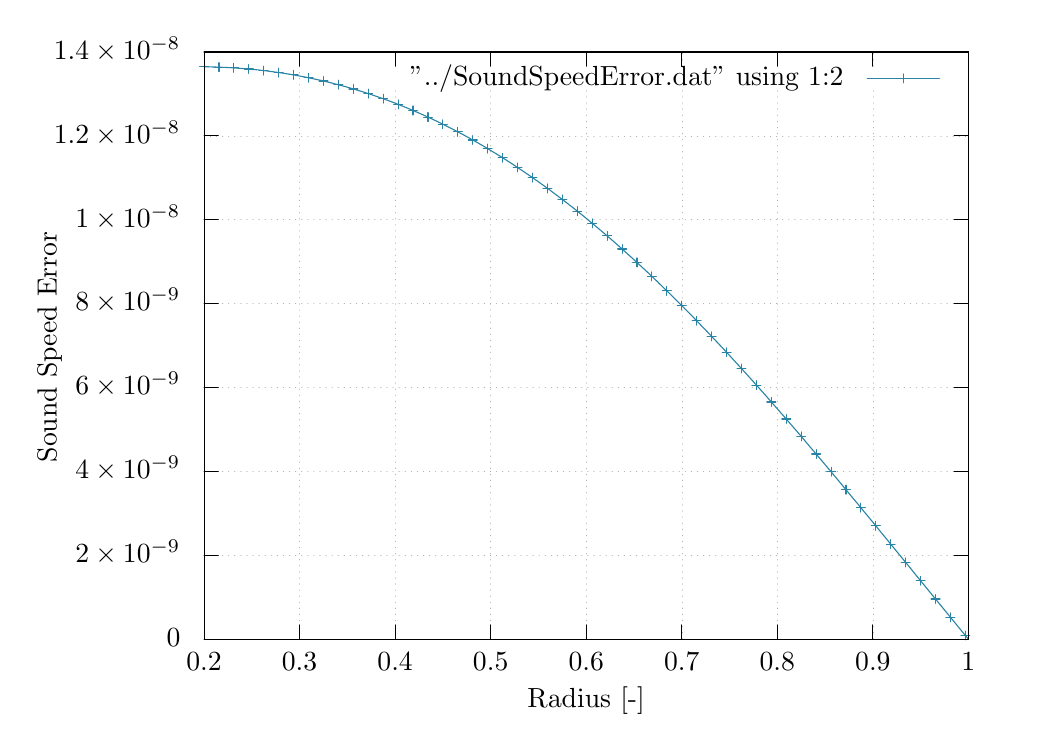
\begin{tikzpicture}[gnuplot]
%% generated with GNUPLOT 5.2p8 (Lua 5.3; terminal rev. Nov 2018, script rev. 108)
%% Wed 01 Sep 2021 01:14:21 AM EDT
\path (0.000,0.000) rectangle (12.500,8.750);
\gpcolor{color=gp lt color axes}
\gpsetlinetype{gp lt axes}
\gpsetdashtype{gp dt axes}
\gpsetlinewidth{0.50}
\draw[gp path] (2.240,0.985)--(11.947,0.985);
\gpcolor{color=gp lt color border}
\gpsetlinetype{gp lt border}
\gpsetdashtype{gp dt solid}
\gpsetlinewidth{1.00}
\draw[gp path] (2.240,0.985)--(2.420,0.985);
\draw[gp path] (11.947,0.985)--(11.767,0.985);
\node[gp node right] at (2.056,0.985) {$0$};
\gpcolor{color=gp lt color axes}
\gpsetlinetype{gp lt axes}
\gpsetdashtype{gp dt axes}
\gpsetlinewidth{0.50}
\draw[gp path] (2.240,2.050)--(11.947,2.050);
\gpcolor{color=gp lt color border}
\gpsetlinetype{gp lt border}
\gpsetdashtype{gp dt solid}
\gpsetlinewidth{1.00}
\draw[gp path] (2.240,2.050)--(2.420,2.050);
\draw[gp path] (11.947,2.050)--(11.767,2.050);
\node[gp node right] at (2.056,2.050) {$2\times10^{-9}$};
\gpcolor{color=gp lt color axes}
\gpsetlinetype{gp lt axes}
\gpsetdashtype{gp dt axes}
\gpsetlinewidth{0.50}
\draw[gp path] (2.240,3.115)--(11.947,3.115);
\gpcolor{color=gp lt color border}
\gpsetlinetype{gp lt border}
\gpsetdashtype{gp dt solid}
\gpsetlinewidth{1.00}
\draw[gp path] (2.240,3.115)--(2.420,3.115);
\draw[gp path] (11.947,3.115)--(11.767,3.115);
\node[gp node right] at (2.056,3.115) {$4\times10^{-9}$};
\gpcolor{color=gp lt color axes}
\gpsetlinetype{gp lt axes}
\gpsetdashtype{gp dt axes}
\gpsetlinewidth{0.50}
\draw[gp path] (2.240,4.180)--(11.947,4.180);
\gpcolor{color=gp lt color border}
\gpsetlinetype{gp lt border}
\gpsetdashtype{gp dt solid}
\gpsetlinewidth{1.00}
\draw[gp path] (2.240,4.180)--(2.420,4.180);
\draw[gp path] (11.947,4.180)--(11.767,4.180);
\node[gp node right] at (2.056,4.180) {$6\times10^{-9}$};
\gpcolor{color=gp lt color axes}
\gpsetlinetype{gp lt axes}
\gpsetdashtype{gp dt axes}
\gpsetlinewidth{0.50}
\draw[gp path] (2.240,5.246)--(11.947,5.246);
\gpcolor{color=gp lt color border}
\gpsetlinetype{gp lt border}
\gpsetdashtype{gp dt solid}
\gpsetlinewidth{1.00}
\draw[gp path] (2.240,5.246)--(2.420,5.246);
\draw[gp path] (11.947,5.246)--(11.767,5.246);
\node[gp node right] at (2.056,5.246) {$8\times10^{-9}$};
\gpcolor{color=gp lt color axes}
\gpsetlinetype{gp lt axes}
\gpsetdashtype{gp dt axes}
\gpsetlinewidth{0.50}
\draw[gp path] (2.240,6.311)--(11.947,6.311);
\gpcolor{color=gp lt color border}
\gpsetlinetype{gp lt border}
\gpsetdashtype{gp dt solid}
\gpsetlinewidth{1.00}
\draw[gp path] (2.240,6.311)--(2.420,6.311);
\draw[gp path] (11.947,6.311)--(11.767,6.311);
\node[gp node right] at (2.056,6.311) {$1\times10^{-8}$};
\gpcolor{color=gp lt color axes}
\gpsetlinetype{gp lt axes}
\gpsetdashtype{gp dt axes}
\gpsetlinewidth{0.50}
\draw[gp path] (2.240,7.376)--(11.947,7.376);
\gpcolor{color=gp lt color border}
\gpsetlinetype{gp lt border}
\gpsetdashtype{gp dt solid}
\gpsetlinewidth{1.00}
\draw[gp path] (2.240,7.376)--(2.420,7.376);
\draw[gp path] (11.947,7.376)--(11.767,7.376);
\node[gp node right] at (2.056,7.376) {$1.2\times10^{-8}$};
\gpcolor{color=gp lt color axes}
\gpsetlinetype{gp lt axes}
\gpsetdashtype{gp dt axes}
\gpsetlinewidth{0.50}
\draw[gp path] (2.240,8.441)--(11.947,8.441);
\gpcolor{color=gp lt color border}
\gpsetlinetype{gp lt border}
\gpsetdashtype{gp dt solid}
\gpsetlinewidth{1.00}
\draw[gp path] (2.240,8.441)--(2.420,8.441);
\draw[gp path] (11.947,8.441)--(11.767,8.441);
\node[gp node right] at (2.056,8.441) {$1.4\times10^{-8}$};
\gpcolor{color=gp lt color axes}
\gpsetlinetype{gp lt axes}
\gpsetdashtype{gp dt axes}
\gpsetlinewidth{0.50}
\draw[gp path] (2.240,0.985)--(2.240,8.441);
\gpcolor{color=gp lt color border}
\gpsetlinetype{gp lt border}
\gpsetdashtype{gp dt solid}
\gpsetlinewidth{1.00}
\draw[gp path] (2.240,0.985)--(2.240,1.165);
\draw[gp path] (2.240,8.441)--(2.240,8.261);
\node[gp node center] at (2.240,0.677) {$0.2$};
\gpcolor{color=gp lt color axes}
\gpsetlinetype{gp lt axes}
\gpsetdashtype{gp dt axes}
\gpsetlinewidth{0.50}
\draw[gp path] (3.453,0.985)--(3.453,8.441);
\gpcolor{color=gp lt color border}
\gpsetlinetype{gp lt border}
\gpsetdashtype{gp dt solid}
\gpsetlinewidth{1.00}
\draw[gp path] (3.453,0.985)--(3.453,1.165);
\draw[gp path] (3.453,8.441)--(3.453,8.261);
\node[gp node center] at (3.453,0.677) {$0.3$};
\gpcolor{color=gp lt color axes}
\gpsetlinetype{gp lt axes}
\gpsetdashtype{gp dt axes}
\gpsetlinewidth{0.50}
\draw[gp path] (4.667,0.985)--(4.667,7.953);
\draw[gp path] (4.667,8.261)--(4.667,8.441);
\gpcolor{color=gp lt color border}
\gpsetlinetype{gp lt border}
\gpsetdashtype{gp dt solid}
\gpsetlinewidth{1.00}
\draw[gp path] (4.667,0.985)--(4.667,1.165);
\draw[gp path] (4.667,8.441)--(4.667,8.261);
\node[gp node center] at (4.667,0.677) {$0.4$};
\gpcolor{color=gp lt color axes}
\gpsetlinetype{gp lt axes}
\gpsetdashtype{gp dt axes}
\gpsetlinewidth{0.50}
\draw[gp path] (5.880,0.985)--(5.880,7.953);
\draw[gp path] (5.880,8.261)--(5.880,8.441);
\gpcolor{color=gp lt color border}
\gpsetlinetype{gp lt border}
\gpsetdashtype{gp dt solid}
\gpsetlinewidth{1.00}
\draw[gp path] (5.880,0.985)--(5.880,1.165);
\draw[gp path] (5.880,8.441)--(5.880,8.261);
\node[gp node center] at (5.880,0.677) {$0.5$};
\gpcolor{color=gp lt color axes}
\gpsetlinetype{gp lt axes}
\gpsetdashtype{gp dt axes}
\gpsetlinewidth{0.50}
\draw[gp path] (7.094,0.985)--(7.094,7.953);
\draw[gp path] (7.094,8.261)--(7.094,8.441);
\gpcolor{color=gp lt color border}
\gpsetlinetype{gp lt border}
\gpsetdashtype{gp dt solid}
\gpsetlinewidth{1.00}
\draw[gp path] (7.094,0.985)--(7.094,1.165);
\draw[gp path] (7.094,8.441)--(7.094,8.261);
\node[gp node center] at (7.094,0.677) {$0.6$};
\gpcolor{color=gp lt color axes}
\gpsetlinetype{gp lt axes}
\gpsetdashtype{gp dt axes}
\gpsetlinewidth{0.50}
\draw[gp path] (8.307,0.985)--(8.307,7.953);
\draw[gp path] (8.307,8.261)--(8.307,8.441);
\gpcolor{color=gp lt color border}
\gpsetlinetype{gp lt border}
\gpsetdashtype{gp dt solid}
\gpsetlinewidth{1.00}
\draw[gp path] (8.307,0.985)--(8.307,1.165);
\draw[gp path] (8.307,8.441)--(8.307,8.261);
\node[gp node center] at (8.307,0.677) {$0.7$};
\gpcolor{color=gp lt color axes}
\gpsetlinetype{gp lt axes}
\gpsetdashtype{gp dt axes}
\gpsetlinewidth{0.50}
\draw[gp path] (9.520,0.985)--(9.520,7.953);
\draw[gp path] (9.520,8.261)--(9.520,8.441);
\gpcolor{color=gp lt color border}
\gpsetlinetype{gp lt border}
\gpsetdashtype{gp dt solid}
\gpsetlinewidth{1.00}
\draw[gp path] (9.520,0.985)--(9.520,1.165);
\draw[gp path] (9.520,8.441)--(9.520,8.261);
\node[gp node center] at (9.520,0.677) {$0.8$};
\gpcolor{color=gp lt color axes}
\gpsetlinetype{gp lt axes}
\gpsetdashtype{gp dt axes}
\gpsetlinewidth{0.50}
\draw[gp path] (10.734,0.985)--(10.734,7.953);
\draw[gp path] (10.734,8.261)--(10.734,8.441);
\gpcolor{color=gp lt color border}
\gpsetlinetype{gp lt border}
\gpsetdashtype{gp dt solid}
\gpsetlinewidth{1.00}
\draw[gp path] (10.734,0.985)--(10.734,1.165);
\draw[gp path] (10.734,8.441)--(10.734,8.261);
\node[gp node center] at (10.734,0.677) {$0.9$};
\gpcolor{color=gp lt color axes}
\gpsetlinetype{gp lt axes}
\gpsetdashtype{gp dt axes}
\gpsetlinewidth{0.50}
\draw[gp path] (11.947,0.985)--(11.947,8.441);
\gpcolor{color=gp lt color border}
\gpsetlinetype{gp lt border}
\gpsetdashtype{gp dt solid}
\gpsetlinewidth{1.00}
\draw[gp path] (11.947,0.985)--(11.947,1.165);
\draw[gp path] (11.947,8.441)--(11.947,8.261);
\node[gp node center] at (11.947,0.677) {$1$};
\draw[gp path] (2.240,8.441)--(2.240,0.985)--(11.947,0.985)--(11.947,8.441)--cycle;
\node[gp node center,rotate=-270] at (0.292,4.713) {Sound Speed Error};
\node[gp node center] at (7.093,0.215) {Radius [-]};
\node[gp node right] at (10.479,8.107) {"../SoundSpeedError.dat" using 1:2};
\gpcolor{rgb color={0.165,0.518,0.647}}
\draw[gp path] (10.663,8.107)--(11.579,8.107);
\draw[gp path] (2.240,8.253)--(2.259,8.253)--(2.278,8.253)--(2.297,8.253)--(2.316,8.252)%
  --(2.335,8.252)--(2.354,8.251)--(2.373,8.251)--(2.392,8.250)--(2.411,8.249)--(2.430,8.249)%
  --(2.449,8.248)--(2.468,8.247)--(2.486,8.246)--(2.505,8.246)--(2.524,8.245)--(2.543,8.244)%
  --(2.562,8.243)--(2.581,8.242)--(2.600,8.240)--(2.619,8.239)--(2.638,8.238)--(2.657,8.237)%
  --(2.676,8.235)--(2.695,8.234)--(2.714,8.233)--(2.733,8.231)--(2.752,8.230)--(2.771,8.228)%
  --(2.790,8.226)--(2.809,8.225)--(2.828,8.223)--(2.847,8.221)--(2.866,8.219)--(2.885,8.218)%
  --(2.904,8.216)--(2.923,8.214)--(2.941,8.212)--(2.960,8.209)--(2.979,8.207)--(2.998,8.205)%
  --(3.017,8.203)--(3.036,8.201)--(3.055,8.198)--(3.074,8.196)--(3.093,8.193)--(3.112,8.191)%
  --(3.131,8.188)--(3.150,8.186)--(3.169,8.183)--(3.188,8.180)--(3.207,8.178)--(3.226,8.175)%
  --(3.245,8.172)--(3.264,8.169)--(3.283,8.166)--(3.302,8.163)--(3.321,8.160)--(3.340,8.157)%
  --(3.359,8.153)--(3.378,8.150)--(3.396,8.147)--(3.415,8.143)--(3.434,8.140)--(3.453,8.136)%
  --(3.472,8.133)--(3.491,8.129)--(3.510,8.126)--(3.529,8.122)--(3.548,8.118)--(3.567,8.114)%
  --(3.586,8.110)--(3.605,8.106)--(3.624,8.102)--(3.643,8.098)--(3.662,8.094)--(3.681,8.090)%
  --(3.700,8.086)--(3.719,8.082)--(3.738,8.077)--(3.757,8.073)--(3.776,8.068)--(3.795,8.064)%
  --(3.814,8.059)--(3.833,8.055)--(3.852,8.050)--(3.870,8.045)--(3.889,8.040)--(3.908,8.035)%
  --(3.927,8.030)--(3.946,8.026)--(3.965,8.020)--(3.984,8.015)--(4.003,8.010)--(4.022,8.005)%
  --(4.041,8.000)--(4.060,7.994)--(4.079,7.989)--(4.098,7.983)--(4.117,7.978)--(4.136,7.972)%
  --(4.155,7.967)--(4.174,7.961)--(4.193,7.955)--(4.212,7.949)--(4.231,7.944)--(4.250,7.938)%
  --(4.269,7.932)--(4.288,7.925)--(4.307,7.919)--(4.325,7.913)--(4.344,7.907)--(4.363,7.901)%
  --(4.382,7.894)--(4.401,7.888)--(4.420,7.881)--(4.439,7.875)--(4.458,7.868)--(4.477,7.861)%
  --(4.496,7.855)--(4.515,7.848)--(4.534,7.841)--(4.553,7.834)--(4.572,7.827)--(4.591,7.820)%
  --(4.610,7.813)--(4.629,7.806)--(4.648,7.798)--(4.667,7.791)--(4.686,7.784)--(4.705,7.776)%
  --(4.724,7.769)--(4.743,7.761)--(4.762,7.754)--(4.781,7.746)--(4.799,7.738)--(4.818,7.731)%
  --(4.837,7.723)--(4.856,7.715)--(4.875,7.707)--(4.894,7.699)--(4.913,7.691)--(4.932,7.682)%
  --(4.951,7.674)--(4.970,7.666)--(4.989,7.657)--(5.008,7.649)--(5.027,7.640)--(5.046,7.632)%
  --(5.065,7.623)--(5.084,7.615)--(5.103,7.606)--(5.122,7.597)--(5.141,7.588)--(5.160,7.579)%
  --(5.179,7.570)--(5.198,7.561)--(5.217,7.552)--(5.236,7.543)--(5.254,7.533)--(5.273,7.524)%
  --(5.292,7.515)--(5.311,7.505)--(5.330,7.496)--(5.349,7.486)--(5.368,7.476)--(5.387,7.467)%
  --(5.406,7.457)--(5.425,7.447)--(5.444,7.437)--(5.463,7.427)--(5.482,7.417)--(5.501,7.407)%
  --(5.520,7.397)--(5.539,7.387)--(5.558,7.376)--(5.577,7.366)--(5.596,7.356)--(5.615,7.345)%
  --(5.634,7.334)--(5.653,7.324)--(5.672,7.313)--(5.691,7.302)--(5.709,7.292)--(5.728,7.281)%
  --(5.747,7.270)--(5.766,7.259)--(5.785,7.248)--(5.804,7.237)--(5.823,7.225)--(5.842,7.214)%
  --(5.861,7.203)--(5.880,7.191)--(5.899,7.180)--(5.918,7.168)--(5.937,7.157)--(5.956,7.145)%
  --(5.975,7.133)--(5.994,7.122)--(6.013,7.110)--(6.032,7.098)--(6.051,7.086)--(6.070,7.074)%
  --(6.089,7.062)--(6.108,7.049)--(6.127,7.037)--(6.146,7.025)--(6.165,7.013)--(6.183,7.000)%
  --(6.202,6.988)--(6.221,6.975)--(6.240,6.962)--(6.259,6.950)--(6.278,6.937)--(6.297,6.924)%
  --(6.316,6.911)--(6.335,6.898)--(6.354,6.885)--(6.373,6.872)--(6.392,6.859)--(6.411,6.846)%
  --(6.430,6.833)--(6.449,6.819)--(6.468,6.806)--(6.487,6.792)--(6.506,6.779)--(6.525,6.765)%
  --(6.544,6.752)--(6.563,6.738)--(6.582,6.724)--(6.601,6.710)--(6.620,6.697)--(6.638,6.683)%
  --(6.657,6.669)--(6.676,6.654)--(6.695,6.640)--(6.714,6.626)--(6.733,6.612)--(6.752,6.597)%
  --(6.771,6.583)--(6.790,6.569)--(6.809,6.554)--(6.828,6.540)--(6.847,6.525)--(6.866,6.510)%
  --(6.885,6.495)--(6.904,6.481)--(6.923,6.466)--(6.942,6.451)--(6.961,6.436)--(6.980,6.421)%
  --(6.999,6.405)--(7.018,6.390)--(7.037,6.375)--(7.056,6.360)--(7.075,6.344)--(7.094,6.329)%
  --(7.112,6.313)--(7.131,6.298)--(7.150,6.282)--(7.169,6.266)--(7.188,6.251)--(7.207,6.235)%
  --(7.226,6.219)--(7.245,6.203)--(7.264,6.187)--(7.283,6.171)--(7.302,6.155)--(7.321,6.139)%
  --(7.340,6.123)--(7.359,6.106)--(7.378,6.090)--(7.397,6.074)--(7.416,6.057)--(7.435,6.041)%
  --(7.454,6.024)--(7.473,6.007)--(7.492,5.991)--(7.511,5.974)--(7.530,5.957)--(7.549,5.940)%
  --(7.567,5.923)--(7.586,5.906)--(7.605,5.889)--(7.624,5.872)--(7.643,5.855)--(7.662,5.838)%
  --(7.681,5.821)--(7.700,5.803)--(7.719,5.786)--(7.738,5.769)--(7.757,5.751)--(7.776,5.733)%
  --(7.795,5.716)--(7.814,5.698)--(7.833,5.681)--(7.852,5.663)--(7.871,5.645)--(7.890,5.627)%
  --(7.909,5.609)--(7.928,5.591)--(7.947,5.573)--(7.966,5.555)--(7.985,5.537)--(8.004,5.519)%
  --(8.022,5.500)--(8.041,5.482)--(8.060,5.464)--(8.079,5.445)--(8.098,5.427)--(8.117,5.408)%
  --(8.136,5.390)--(8.155,5.371)--(8.174,5.353)--(8.193,5.334)--(8.212,5.315)--(8.231,5.296)%
  --(8.250,5.277)--(8.269,5.259)--(8.288,5.240)--(8.307,5.221)--(8.326,5.201)--(8.345,5.182)%
  --(8.364,5.163)--(8.383,5.144)--(8.402,5.125)--(8.421,5.105)--(8.440,5.086)--(8.459,5.067)%
  --(8.478,5.047)--(8.496,5.028)--(8.515,5.008)--(8.534,4.989)--(8.553,4.969)--(8.572,4.949)%
  --(8.591,4.929)--(8.610,4.910)--(8.629,4.890)--(8.648,4.870)--(8.667,4.850)--(8.686,4.830)%
  --(8.705,4.810)--(8.724,4.790)--(8.743,4.770)--(8.762,4.750)--(8.781,4.730)--(8.800,4.709)%
  --(8.819,4.689)--(8.838,4.669)--(8.857,4.648)--(8.876,4.628)--(8.895,4.607)--(8.914,4.587)%
  --(8.933,4.566)--(8.951,4.546)--(8.970,4.525)--(8.989,4.505)--(9.008,4.484)--(9.027,4.463)%
  --(9.046,4.442)--(9.065,4.422)--(9.084,4.401)--(9.103,4.380)--(9.122,4.359)--(9.141,4.338)%
  --(9.160,4.317)--(9.179,4.296)--(9.198,4.275)--(9.217,4.254)--(9.236,4.232)--(9.255,4.211)%
  --(9.274,4.190)--(9.293,4.169)--(9.312,4.147)--(9.331,4.126)--(9.350,4.105)--(9.369,4.083)%
  --(9.388,4.062)--(9.406,4.040)--(9.425,4.019)--(9.444,3.997)--(9.463,3.976)--(9.482,3.954)%
  --(9.501,3.932)--(9.520,3.911)--(9.539,3.889)--(9.558,3.867)--(9.577,3.845)--(9.596,3.824)%
  --(9.615,3.802)--(9.634,3.780)--(9.653,3.758)--(9.672,3.736)--(9.691,3.714)--(9.710,3.692)%
  --(9.729,3.670)--(9.748,3.648)--(9.767,3.626)--(9.786,3.604)--(9.805,3.582)--(9.824,3.559)%
  --(9.843,3.537)--(9.862,3.515)--(9.880,3.493)--(9.899,3.470)--(9.918,3.448)--(9.937,3.426)%
  --(9.956,3.403)--(9.975,3.381)--(9.994,3.359)--(10.013,3.336)--(10.032,3.314)--(10.051,3.291)%
  --(10.070,3.269)--(10.089,3.246)--(10.108,3.224)--(10.127,3.201)--(10.146,3.178)--(10.165,3.156)%
  --(10.184,3.133)--(10.203,3.111)--(10.222,3.088)--(10.241,3.065)--(10.260,3.042)--(10.279,3.020)%
  --(10.298,2.997)--(10.317,2.974)--(10.335,2.951)--(10.354,2.929)--(10.373,2.906)--(10.392,2.883)%
  --(10.411,2.860)--(10.430,2.837)--(10.449,2.814)--(10.468,2.791)--(10.487,2.768)--(10.506,2.745)%
  --(10.525,2.723)--(10.544,2.700)--(10.563,2.677)--(10.582,2.654)--(10.601,2.631)--(10.620,2.607)%
  --(10.639,2.584)--(10.658,2.561)--(10.677,2.538)--(10.696,2.515)--(10.715,2.492)--(10.734,2.469)%
  --(10.753,2.446)--(10.772,2.423)--(10.791,2.400)--(10.809,2.377)--(10.828,2.353)--(10.847,2.330)%
  --(10.866,2.307)--(10.885,2.284)--(10.904,2.261)--(10.923,2.238)--(10.942,2.214)--(10.961,2.191)%
  --(10.980,2.168)--(10.999,2.145)--(11.018,2.121)--(11.037,2.098)--(11.056,2.075)--(11.075,2.052)%
  --(11.094,2.029)--(11.113,2.005)--(11.132,1.982)--(11.151,1.959)--(11.170,1.936)--(11.189,1.912)%
  --(11.208,1.889)--(11.227,1.866)--(11.246,1.843)--(11.264,1.819)--(11.283,1.796)--(11.302,1.773)%
  --(11.321,1.750)--(11.340,1.726)--(11.359,1.703)--(11.378,1.680)--(11.397,1.657)--(11.416,1.633)%
  --(11.435,1.610)--(11.454,1.587)--(11.473,1.564)--(11.492,1.540)--(11.511,1.517)--(11.530,1.494)%
  --(11.549,1.471)--(11.568,1.447)--(11.587,1.424)--(11.606,1.401)--(11.625,1.378)--(11.644,1.355)%
  --(11.663,1.332)--(11.682,1.308)--(11.701,1.285)--(11.719,1.262)--(11.738,1.239)--(11.757,1.216)%
  --(11.776,1.193)--(11.795,1.170)--(11.814,1.146)--(11.833,1.123)--(11.852,1.100)--(11.871,1.077)%
  --(11.890,1.054)--(11.909,1.031)--(11.928,1.008)--(11.947,0.985);
\gpsetpointsize{4.00}
\gppoint{gp mark 1}{(2.240,8.253)}
\gppoint{gp mark 1}{(2.430,8.249)}
\gppoint{gp mark 1}{(2.619,8.239)}
\gppoint{gp mark 1}{(2.809,8.225)}
\gppoint{gp mark 1}{(2.998,8.205)}
\gppoint{gp mark 1}{(3.188,8.180)}
\gppoint{gp mark 1}{(3.378,8.150)}
\gppoint{gp mark 1}{(3.567,8.114)}
\gppoint{gp mark 1}{(3.757,8.073)}
\gppoint{gp mark 1}{(3.946,8.026)}
\gppoint{gp mark 1}{(4.136,7.972)}
\gppoint{gp mark 1}{(4.325,7.913)}
\gppoint{gp mark 1}{(4.515,7.848)}
\gppoint{gp mark 1}{(4.705,7.776)}
\gppoint{gp mark 1}{(4.894,7.699)}
\gppoint{gp mark 1}{(5.084,7.615)}
\gppoint{gp mark 1}{(5.273,7.524)}
\gppoint{gp mark 1}{(5.463,7.427)}
\gppoint{gp mark 1}{(5.653,7.324)}
\gppoint{gp mark 1}{(5.842,7.214)}
\gppoint{gp mark 1}{(6.032,7.098)}
\gppoint{gp mark 1}{(6.221,6.975)}
\gppoint{gp mark 1}{(6.411,6.846)}
\gppoint{gp mark 1}{(6.601,6.710)}
\gppoint{gp mark 1}{(6.790,6.569)}
\gppoint{gp mark 1}{(6.980,6.421)}
\gppoint{gp mark 1}{(7.169,6.266)}
\gppoint{gp mark 1}{(7.359,6.106)}
\gppoint{gp mark 1}{(7.549,5.940)}
\gppoint{gp mark 1}{(7.738,5.769)}
\gppoint{gp mark 1}{(7.928,5.591)}
\gppoint{gp mark 1}{(8.117,5.408)}
\gppoint{gp mark 1}{(8.307,5.221)}
\gppoint{gp mark 1}{(8.496,5.028)}
\gppoint{gp mark 1}{(8.686,4.830)}
\gppoint{gp mark 1}{(8.876,4.628)}
\gppoint{gp mark 1}{(9.065,4.422)}
\gppoint{gp mark 1}{(9.255,4.211)}
\gppoint{gp mark 1}{(9.444,3.997)}
\gppoint{gp mark 1}{(9.634,3.780)}
\gppoint{gp mark 1}{(9.824,3.559)}
\gppoint{gp mark 1}{(10.013,3.336)}
\gppoint{gp mark 1}{(10.203,3.111)}
\gppoint{gp mark 1}{(10.392,2.883)}
\gppoint{gp mark 1}{(10.582,2.654)}
\gppoint{gp mark 1}{(10.772,2.423)}
\gppoint{gp mark 1}{(10.961,2.191)}
\gppoint{gp mark 1}{(11.151,1.959)}
\gppoint{gp mark 1}{(11.340,1.726)}
\gppoint{gp mark 1}{(11.530,1.494)}
\gppoint{gp mark 1}{(11.719,1.262)}
\gppoint{gp mark 1}{(11.909,1.031)}
\gppoint{gp mark 1}{(11.121,8.107)}
\gpcolor{color=gp lt color border}
\draw[gp path] (2.240,8.441)--(2.240,0.985)--(11.947,0.985)--(11.947,8.441)--cycle;
%% coordinates of the plot area
\gpdefrectangularnode{gp plot 1}{\pgfpoint{2.240cm}{0.985cm}}{\pgfpoint{11.947cm}{8.441cm}}
\end{tikzpicture}
%% gnuplot variables
}
    \end{center}
\end{figure}

\begin{figure}
    \begin{center}
        \scalebox{0.75}{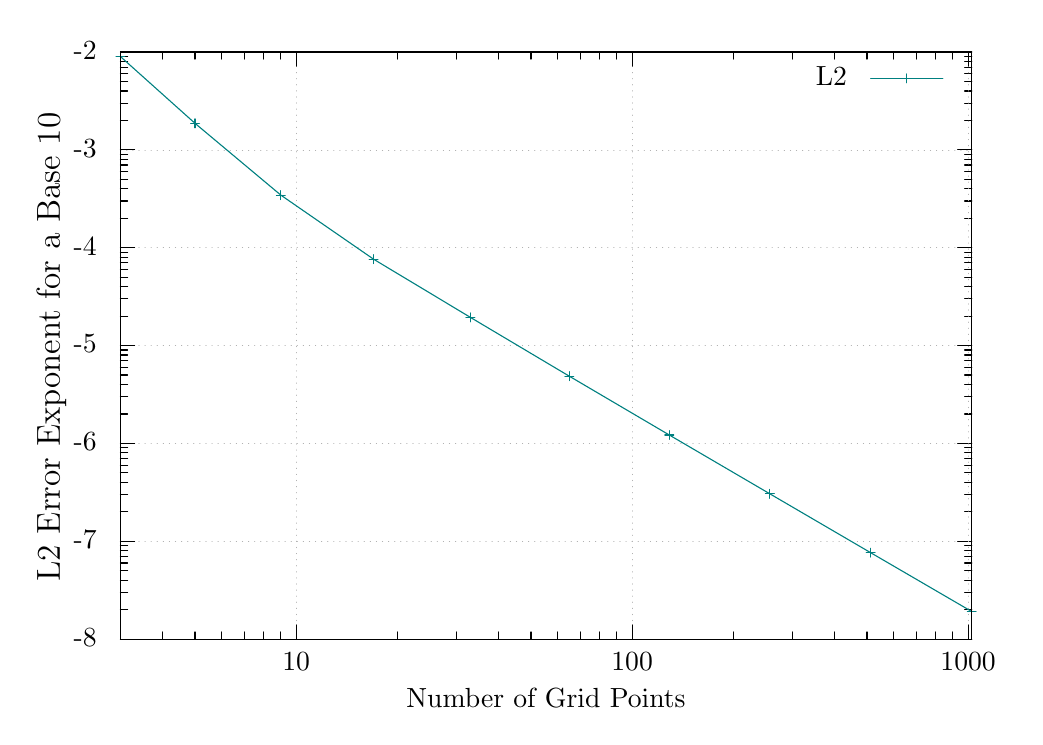
\begin{tikzpicture}[gnuplot]
%% generated with GNUPLOT 5.2p8 (Lua 5.3; terminal rev. Nov 2018, script rev. 108)
%% Tue 21 Sep 2021 05:01:33 PM EDT
\path (0.000,0.000) rectangle (12.500,8.750);
\gpcolor{color=gp lt color axes}
\gpsetlinetype{gp lt axes}
\gpsetdashtype{gp dt axes}
\gpsetlinewidth{0.50}
\draw[gp path] (1.136,0.985)--(11.947,0.985);
\gpcolor{color=gp lt color border}
\gpsetlinetype{gp lt border}
\gpsetdashtype{gp dt solid}
\gpsetlinewidth{1.00}
\draw[gp path] (1.136,0.985)--(1.316,0.985);
\draw[gp path] (11.947,0.985)--(11.767,0.985);
\node[gp node right] at (0.952,0.985) {{-8}};
\draw[gp path] (1.136,1.359)--(1.226,1.359);
\draw[gp path] (11.947,1.359)--(11.857,1.359);
\draw[gp path] (1.136,1.578)--(1.226,1.578);
\draw[gp path] (11.947,1.578)--(11.857,1.578);
\draw[gp path] (1.136,1.733)--(1.226,1.733);
\draw[gp path] (11.947,1.733)--(11.857,1.733);
\draw[gp path] (1.136,1.854)--(1.226,1.854);
\draw[gp path] (11.947,1.854)--(11.857,1.854);
\draw[gp path] (1.136,1.952)--(1.226,1.952);
\draw[gp path] (11.947,1.952)--(11.857,1.952);
\draw[gp path] (1.136,2.035)--(1.226,2.035);
\draw[gp path] (11.947,2.035)--(11.857,2.035);
\draw[gp path] (1.136,2.107)--(1.226,2.107);
\draw[gp path] (11.947,2.107)--(11.857,2.107);
\draw[gp path] (1.136,2.171)--(1.226,2.171);
\draw[gp path] (11.947,2.171)--(11.857,2.171);
\gpcolor{color=gp lt color axes}
\gpsetlinetype{gp lt axes}
\gpsetdashtype{gp dt axes}
\gpsetlinewidth{0.50}
\draw[gp path] (1.136,2.228)--(11.947,2.228);
\gpcolor{color=gp lt color border}
\gpsetlinetype{gp lt border}
\gpsetdashtype{gp dt solid}
\gpsetlinewidth{1.00}
\draw[gp path] (1.136,2.228)--(1.316,2.228);
\draw[gp path] (11.947,2.228)--(11.767,2.228);
\node[gp node right] at (0.952,2.228) {{-7}};
\draw[gp path] (1.136,2.602)--(1.226,2.602);
\draw[gp path] (11.947,2.602)--(11.857,2.602);
\draw[gp path] (1.136,2.821)--(1.226,2.821);
\draw[gp path] (11.947,2.821)--(11.857,2.821);
\draw[gp path] (1.136,2.976)--(1.226,2.976);
\draw[gp path] (11.947,2.976)--(11.857,2.976);
\draw[gp path] (1.136,3.096)--(1.226,3.096);
\draw[gp path] (11.947,3.096)--(11.857,3.096);
\draw[gp path] (1.136,3.195)--(1.226,3.195);
\draw[gp path] (11.947,3.195)--(11.857,3.195);
\draw[gp path] (1.136,3.278)--(1.226,3.278);
\draw[gp path] (11.947,3.278)--(11.857,3.278);
\draw[gp path] (1.136,3.350)--(1.226,3.350);
\draw[gp path] (11.947,3.350)--(11.857,3.350);
\draw[gp path] (1.136,3.413)--(1.226,3.413);
\draw[gp path] (11.947,3.413)--(11.857,3.413);
\gpcolor{color=gp lt color axes}
\gpsetlinetype{gp lt axes}
\gpsetdashtype{gp dt axes}
\gpsetlinewidth{0.50}
\draw[gp path] (1.136,3.470)--(11.947,3.470);
\gpcolor{color=gp lt color border}
\gpsetlinetype{gp lt border}
\gpsetdashtype{gp dt solid}
\gpsetlinewidth{1.00}
\draw[gp path] (1.136,3.470)--(1.316,3.470);
\draw[gp path] (11.947,3.470)--(11.767,3.470);
\node[gp node right] at (0.952,3.470) {{-6}};
\draw[gp path] (1.136,3.844)--(1.226,3.844);
\draw[gp path] (11.947,3.844)--(11.857,3.844);
\draw[gp path] (1.136,4.063)--(1.226,4.063);
\draw[gp path] (11.947,4.063)--(11.857,4.063);
\draw[gp path] (1.136,4.218)--(1.226,4.218);
\draw[gp path] (11.947,4.218)--(11.857,4.218);
\draw[gp path] (1.136,4.339)--(1.226,4.339);
\draw[gp path] (11.947,4.339)--(11.857,4.339);
\draw[gp path] (1.136,4.437)--(1.226,4.437);
\draw[gp path] (11.947,4.437)--(11.857,4.437);
\draw[gp path] (1.136,4.521)--(1.226,4.521);
\draw[gp path] (11.947,4.521)--(11.857,4.521);
\draw[gp path] (1.136,4.593)--(1.226,4.593);
\draw[gp path] (11.947,4.593)--(11.857,4.593);
\draw[gp path] (1.136,4.656)--(1.226,4.656);
\draw[gp path] (11.947,4.656)--(11.857,4.656);
\gpcolor{color=gp lt color axes}
\gpsetlinetype{gp lt axes}
\gpsetdashtype{gp dt axes}
\gpsetlinewidth{0.50}
\draw[gp path] (1.136,4.713)--(11.947,4.713);
\gpcolor{color=gp lt color border}
\gpsetlinetype{gp lt border}
\gpsetdashtype{gp dt solid}
\gpsetlinewidth{1.00}
\draw[gp path] (1.136,4.713)--(1.316,4.713);
\draw[gp path] (11.947,4.713)--(11.767,4.713);
\node[gp node right] at (0.952,4.713) {{-5}};
\draw[gp path] (1.136,5.087)--(1.226,5.087);
\draw[gp path] (11.947,5.087)--(11.857,5.087);
\draw[gp path] (1.136,5.306)--(1.226,5.306);
\draw[gp path] (11.947,5.306)--(11.857,5.306);
\draw[gp path] (1.136,5.461)--(1.226,5.461);
\draw[gp path] (11.947,5.461)--(11.857,5.461);
\draw[gp path] (1.136,5.582)--(1.226,5.582);
\draw[gp path] (11.947,5.582)--(11.857,5.582);
\draw[gp path] (1.136,5.680)--(1.226,5.680);
\draw[gp path] (11.947,5.680)--(11.857,5.680);
\draw[gp path] (1.136,5.763)--(1.226,5.763);
\draw[gp path] (11.947,5.763)--(11.857,5.763);
\draw[gp path] (1.136,5.835)--(1.226,5.835);
\draw[gp path] (11.947,5.835)--(11.857,5.835);
\draw[gp path] (1.136,5.899)--(1.226,5.899);
\draw[gp path] (11.947,5.899)--(11.857,5.899);
\gpcolor{color=gp lt color axes}
\gpsetlinetype{gp lt axes}
\gpsetdashtype{gp dt axes}
\gpsetlinewidth{0.50}
\draw[gp path] (1.136,5.956)--(11.947,5.956);
\gpcolor{color=gp lt color border}
\gpsetlinetype{gp lt border}
\gpsetdashtype{gp dt solid}
\gpsetlinewidth{1.00}
\draw[gp path] (1.136,5.956)--(1.316,5.956);
\draw[gp path] (11.947,5.956)--(11.767,5.956);
\node[gp node right] at (0.952,5.956) {{-4}};
\draw[gp path] (1.136,6.330)--(1.226,6.330);
\draw[gp path] (11.947,6.330)--(11.857,6.330);
\draw[gp path] (1.136,6.549)--(1.226,6.549);
\draw[gp path] (11.947,6.549)--(11.857,6.549);
\draw[gp path] (1.136,6.704)--(1.226,6.704);
\draw[gp path] (11.947,6.704)--(11.857,6.704);
\draw[gp path] (1.136,6.824)--(1.226,6.824);
\draw[gp path] (11.947,6.824)--(11.857,6.824);
\draw[gp path] (1.136,6.923)--(1.226,6.923);
\draw[gp path] (11.947,6.923)--(11.857,6.923);
\draw[gp path] (1.136,7.006)--(1.226,7.006);
\draw[gp path] (11.947,7.006)--(11.857,7.006);
\draw[gp path] (1.136,7.078)--(1.226,7.078);
\draw[gp path] (11.947,7.078)--(11.857,7.078);
\draw[gp path] (1.136,7.141)--(1.226,7.141);
\draw[gp path] (11.947,7.141)--(11.857,7.141);
\gpcolor{color=gp lt color axes}
\gpsetlinetype{gp lt axes}
\gpsetdashtype{gp dt axes}
\gpsetlinewidth{0.50}
\draw[gp path] (1.136,7.198)--(11.947,7.198);
\gpcolor{color=gp lt color border}
\gpsetlinetype{gp lt border}
\gpsetdashtype{gp dt solid}
\gpsetlinewidth{1.00}
\draw[gp path] (1.136,7.198)--(1.316,7.198);
\draw[gp path] (11.947,7.198)--(11.767,7.198);
\node[gp node right] at (0.952,7.198) {{-3}};
\draw[gp path] (1.136,7.572)--(1.226,7.572);
\draw[gp path] (11.947,7.572)--(11.857,7.572);
\draw[gp path] (1.136,7.791)--(1.226,7.791);
\draw[gp path] (11.947,7.791)--(11.857,7.791);
\draw[gp path] (1.136,7.946)--(1.226,7.946);
\draw[gp path] (11.947,7.946)--(11.857,7.946);
\draw[gp path] (1.136,8.067)--(1.226,8.067);
\draw[gp path] (11.947,8.067)--(11.857,8.067);
\draw[gp path] (1.136,8.165)--(1.226,8.165);
\draw[gp path] (11.947,8.165)--(11.857,8.165);
\draw[gp path] (1.136,8.249)--(1.226,8.249);
\draw[gp path] (11.947,8.249)--(11.857,8.249);
\draw[gp path] (1.136,8.321)--(1.226,8.321);
\draw[gp path] (11.947,8.321)--(11.857,8.321);
\draw[gp path] (1.136,8.384)--(1.226,8.384);
\draw[gp path] (11.947,8.384)--(11.857,8.384);
\gpcolor{color=gp lt color axes}
\gpsetlinetype{gp lt axes}
\gpsetdashtype{gp dt axes}
\gpsetlinewidth{0.50}
\draw[gp path] (1.136,8.441)--(11.947,8.441);
\gpcolor{color=gp lt color border}
\gpsetlinetype{gp lt border}
\gpsetdashtype{gp dt solid}
\gpsetlinewidth{1.00}
\draw[gp path] (1.136,8.441)--(1.316,8.441);
\draw[gp path] (11.947,8.441)--(11.767,8.441);
\node[gp node right] at (0.952,8.441) {{-2}};
\draw[gp path] (1.136,0.985)--(1.136,1.075);
\draw[gp path] (1.136,8.441)--(1.136,8.351);
\draw[gp path] (1.669,0.985)--(1.669,1.075);
\draw[gp path] (1.669,8.441)--(1.669,8.351);
\draw[gp path] (2.083,0.985)--(2.083,1.075);
\draw[gp path] (2.083,8.441)--(2.083,8.351);
\draw[gp path] (2.421,0.985)--(2.421,1.075);
\draw[gp path] (2.421,8.441)--(2.421,8.351);
\draw[gp path] (2.706,0.985)--(2.706,1.075);
\draw[gp path] (2.706,8.441)--(2.706,8.351);
\draw[gp path] (2.954,0.985)--(2.954,1.075);
\draw[gp path] (2.954,8.441)--(2.954,8.351);
\draw[gp path] (3.172,0.985)--(3.172,1.075);
\draw[gp path] (3.172,8.441)--(3.172,8.351);
\gpcolor{color=gp lt color axes}
\gpsetlinetype{gp lt axes}
\gpsetdashtype{gp dt axes}
\gpsetlinewidth{0.50}
\draw[gp path] (3.367,0.985)--(3.367,8.441);
\gpcolor{color=gp lt color border}
\gpsetlinetype{gp lt border}
\gpsetdashtype{gp dt solid}
\gpsetlinewidth{1.00}
\draw[gp path] (3.367,0.985)--(3.367,1.165);
\draw[gp path] (3.367,8.441)--(3.367,8.261);
\node[gp node center] at (3.367,0.677) {$10$};
\draw[gp path] (4.652,0.985)--(4.652,1.075);
\draw[gp path] (4.652,8.441)--(4.652,8.351);
\draw[gp path] (5.403,0.985)--(5.403,1.075);
\draw[gp path] (5.403,8.441)--(5.403,8.351);
\draw[gp path] (5.936,0.985)--(5.936,1.075);
\draw[gp path] (5.936,8.441)--(5.936,8.351);
\draw[gp path] (6.350,0.985)--(6.350,1.075);
\draw[gp path] (6.350,8.441)--(6.350,8.351);
\draw[gp path] (6.688,0.985)--(6.688,1.075);
\draw[gp path] (6.688,8.441)--(6.688,8.351);
\draw[gp path] (6.973,0.985)--(6.973,1.075);
\draw[gp path] (6.973,8.441)--(6.973,8.351);
\draw[gp path] (7.221,0.985)--(7.221,1.075);
\draw[gp path] (7.221,8.441)--(7.221,8.351);
\draw[gp path] (7.439,0.985)--(7.439,1.075);
\draw[gp path] (7.439,8.441)--(7.439,8.351);
\gpcolor{color=gp lt color axes}
\gpsetlinetype{gp lt axes}
\gpsetdashtype{gp dt axes}
\gpsetlinewidth{0.50}
\draw[gp path] (7.634,0.985)--(7.634,8.441);
\gpcolor{color=gp lt color border}
\gpsetlinetype{gp lt border}
\gpsetdashtype{gp dt solid}
\gpsetlinewidth{1.00}
\draw[gp path] (7.634,0.985)--(7.634,1.165);
\draw[gp path] (7.634,8.441)--(7.634,8.261);
\node[gp node center] at (7.634,0.677) {$100$};
\draw[gp path] (8.919,0.985)--(8.919,1.075);
\draw[gp path] (8.919,8.441)--(8.919,8.351);
\draw[gp path] (9.670,0.985)--(9.670,1.075);
\draw[gp path] (9.670,8.441)--(9.670,8.351);
\draw[gp path] (10.203,0.985)--(10.203,1.075);
\draw[gp path] (10.203,8.441)--(10.203,8.351);
\draw[gp path] (10.617,0.985)--(10.617,1.075);
\draw[gp path] (10.617,8.441)--(10.617,8.351);
\draw[gp path] (10.955,0.985)--(10.955,1.075);
\draw[gp path] (10.955,8.441)--(10.955,8.351);
\draw[gp path] (11.240,0.985)--(11.240,1.075);
\draw[gp path] (11.240,8.441)--(11.240,8.351);
\draw[gp path] (11.488,0.985)--(11.488,1.075);
\draw[gp path] (11.488,8.441)--(11.488,8.351);
\draw[gp path] (11.706,0.985)--(11.706,1.075);
\draw[gp path] (11.706,8.441)--(11.706,8.351);
\gpcolor{color=gp lt color axes}
\gpsetlinetype{gp lt axes}
\gpsetdashtype{gp dt axes}
\gpsetlinewidth{0.50}
\draw[gp path] (11.901,0.985)--(11.901,8.441);
\gpcolor{color=gp lt color border}
\gpsetlinetype{gp lt border}
\gpsetdashtype{gp dt solid}
\gpsetlinewidth{1.00}
\draw[gp path] (11.901,0.985)--(11.901,1.165);
\draw[gp path] (11.901,8.441)--(11.901,8.261);
\node[gp node center] at (11.901,0.677) {$1000$};
\draw[gp path] (1.136,8.441)--(1.136,0.985)--(11.947,0.985)--(11.947,8.441)--cycle;
\node[gp node center,rotate=-270,font={\fontsize{12.0pt}{14.4pt}\selectfont}] at (0.292,4.713) {L2 Error Exponent for a Base 10};
\node[gp node center] at (6.541,0.215) {Number of Grid Points};
\node[gp node right] at (10.479,8.107) {L2};
\gpcolor{rgb color={0.000,0.502,0.502}}
\draw[gp path] (10.663,8.107)--(11.579,8.107);
\draw[gp path] (1.136,8.383)--(2.083,7.535)--(3.172,6.624)--(4.350,5.810)--(5.580,5.071)%
  --(6.836,4.324)--(8.106,3.577)--(9.383,2.830)--(10.664,2.082)--(11.947,1.335);
\gpsetpointsize{4.00}
\gppoint{gp mark 1}{(1.136,8.383)}
\gppoint{gp mark 1}{(2.083,7.535)}
\gppoint{gp mark 1}{(3.172,6.624)}
\gppoint{gp mark 1}{(4.350,5.810)}
\gppoint{gp mark 1}{(5.580,5.071)}
\gppoint{gp mark 1}{(6.836,4.324)}
\gppoint{gp mark 1}{(8.106,3.577)}
\gppoint{gp mark 1}{(9.383,2.830)}
\gppoint{gp mark 1}{(10.664,2.082)}
\gppoint{gp mark 1}{(11.947,1.335)}
\gppoint{gp mark 1}{(11.121,8.107)}
\gpcolor{color=gp lt color border}
\draw[gp path] (1.136,8.441)--(1.136,0.985)--(11.947,0.985)--(11.947,8.441)--cycle;
%% coordinates of the plot area
\gpdefrectangularnode{gp plot 1}{\pgfpoint{1.136cm}{0.985cm}}{\pgfpoint{11.947cm}{8.441cm}}
\end{tikzpicture}
%% gnuplot variables
}
    \end{center}
\end{figure}

\begin{figure}
    \begin{center}
        \scalebox{0.75}{% This file was created with tikzplotlib v0.9.12.
\begin{tikzpicture}

\definecolor{color0}{rgb}{0.12156862745098,0.466666666666667,0.705882352941177}

\begin{groupplot}[group style={group size=1 by 2}]
\nextgroupplot[
axis line style={white!15!black},
legend cell align={left},
legend style={fill opacity=0.8, draw opacity=1, text opacity=1, draw=none},
log basis y={10},
scaled x ticks=manual:{}{\pgfmathparse{#1}},
tick align=outside,
tick pos=left,
title={Rate Of Convergence},
x grid style={white!80!black},
xmin=0.49602339181245, xmax=0.60495126705655,
xtick style={color=white!15!black},
xticklabels={},
y grid style={white!80!black},
ymin=1.93465772282466, ymax=2.50490389113768,
ymode=log,
ytick style={color=white!15!black}
]
\addplot [semithick, color0]
table {%
0.6 2.220755792495
0.555555555556 2.163324274032
0.529411764706 2.475663773488
0.515151515152 1.957508006467
0.507692307692 1.997639457419
0.503875968992 1.996551880759
0.501945525292 1.997726606828
0.500974658869 1.998727064418
};
\addlegendentry{Speed Of Sound}

\nextgroupplot[
axis line style={white!15!black},
legend cell align={left},
legend style={fill opacity=0.8, draw opacity=1, text opacity=1, draw=none},
log basis y={10},
tick align=outside,
tick pos=left,
x grid style={white!80!black},
xlabel={Del r},
xmin=0.49602339181245, xmax=0.60495126705655,
xtick style={color=white!15!black},
y grid style={white!80!black},
ymin=0.362953235346687, ymax=0.506191289267272,
ymode=log,
ytick style={color=white!15!black}
]
\addplot [semithick, color0]
table {%
0.6 0.368482797082
0.555555555556 0.423998453276
0.529411764706 0.458768919907
0.515151515152 0.478465639055
0.507692307692 0.488986846835
0.503875968992 0.494429721197
0.501945525292 0.497198646885
0.500974658869 0.498595233207
};
\addlegendentry{LEE}
\end{groupplot}

\end{tikzpicture}
}
    \end{center}
\end{figure}

\begin{figure}
    \begin{center}
        \scalebox{0.75}{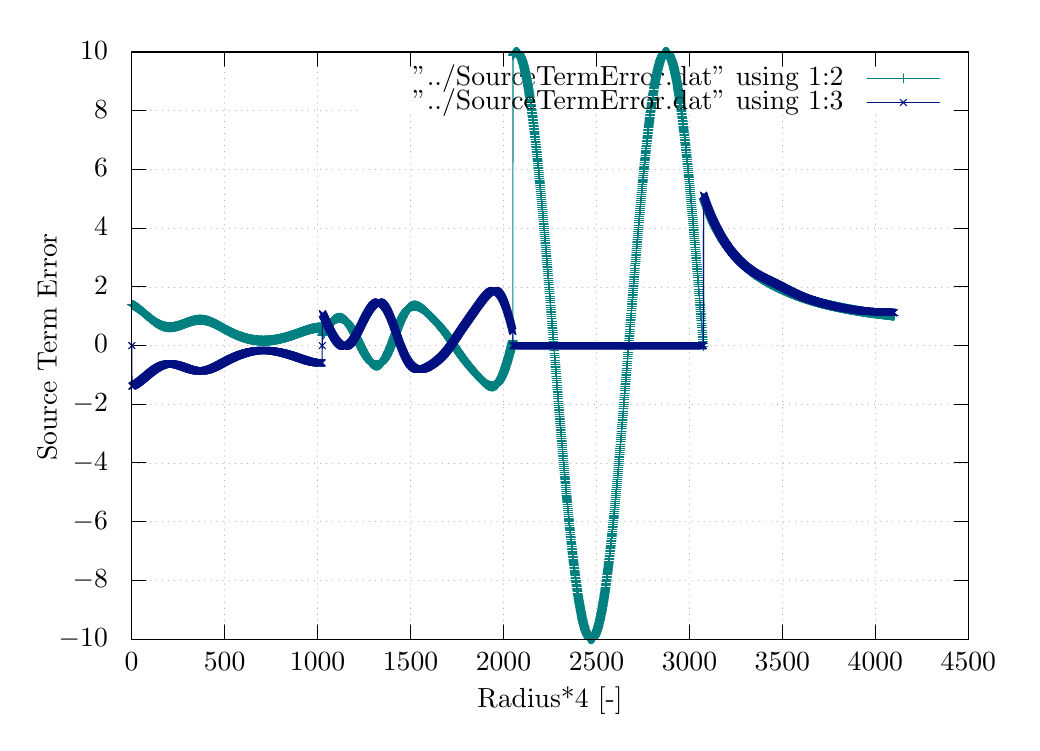
\begin{tikzpicture}[gnuplot]
%% generated with GNUPLOT 5.2p8 (Lua 5.3; terminal rev. Nov 2018, script rev. 108)
%% Tue 14 Sep 2021 10:12:40 AM EDT
\path (0.000,0.000) rectangle (12.500,8.750);
\gpcolor{color=gp lt color axes}
\gpsetlinetype{gp lt axes}
\gpsetdashtype{gp dt axes}
\gpsetlinewidth{0.50}
\draw[gp path] (1.320,0.985)--(11.947,0.985);
\gpcolor{color=gp lt color border}
\gpsetlinetype{gp lt border}
\gpsetdashtype{gp dt solid}
\gpsetlinewidth{1.00}
\draw[gp path] (1.320,0.985)--(1.500,0.985);
\draw[gp path] (11.947,0.985)--(11.767,0.985);
\node[gp node right] at (1.136,0.985) {$-10$};
\gpcolor{color=gp lt color axes}
\gpsetlinetype{gp lt axes}
\gpsetdashtype{gp dt axes}
\gpsetlinewidth{0.50}
\draw[gp path] (1.320,1.731)--(11.947,1.731);
\gpcolor{color=gp lt color border}
\gpsetlinetype{gp lt border}
\gpsetdashtype{gp dt solid}
\gpsetlinewidth{1.00}
\draw[gp path] (1.320,1.731)--(1.500,1.731);
\draw[gp path] (11.947,1.731)--(11.767,1.731);
\node[gp node right] at (1.136,1.731) {$-8$};
\gpcolor{color=gp lt color axes}
\gpsetlinetype{gp lt axes}
\gpsetdashtype{gp dt axes}
\gpsetlinewidth{0.50}
\draw[gp path] (1.320,2.476)--(11.947,2.476);
\gpcolor{color=gp lt color border}
\gpsetlinetype{gp lt border}
\gpsetdashtype{gp dt solid}
\gpsetlinewidth{1.00}
\draw[gp path] (1.320,2.476)--(1.500,2.476);
\draw[gp path] (11.947,2.476)--(11.767,2.476);
\node[gp node right] at (1.136,2.476) {$-6$};
\gpcolor{color=gp lt color axes}
\gpsetlinetype{gp lt axes}
\gpsetdashtype{gp dt axes}
\gpsetlinewidth{0.50}
\draw[gp path] (1.320,3.222)--(11.947,3.222);
\gpcolor{color=gp lt color border}
\gpsetlinetype{gp lt border}
\gpsetdashtype{gp dt solid}
\gpsetlinewidth{1.00}
\draw[gp path] (1.320,3.222)--(1.500,3.222);
\draw[gp path] (11.947,3.222)--(11.767,3.222);
\node[gp node right] at (1.136,3.222) {$-4$};
\gpcolor{color=gp lt color axes}
\gpsetlinetype{gp lt axes}
\gpsetdashtype{gp dt axes}
\gpsetlinewidth{0.50}
\draw[gp path] (1.320,3.967)--(11.947,3.967);
\gpcolor{color=gp lt color border}
\gpsetlinetype{gp lt border}
\gpsetdashtype{gp dt solid}
\gpsetlinewidth{1.00}
\draw[gp path] (1.320,3.967)--(1.500,3.967);
\draw[gp path] (11.947,3.967)--(11.767,3.967);
\node[gp node right] at (1.136,3.967) {$-2$};
\gpcolor{color=gp lt color axes}
\gpsetlinetype{gp lt axes}
\gpsetdashtype{gp dt axes}
\gpsetlinewidth{0.50}
\draw[gp path] (1.320,4.713)--(11.947,4.713);
\gpcolor{color=gp lt color border}
\gpsetlinetype{gp lt border}
\gpsetdashtype{gp dt solid}
\gpsetlinewidth{1.00}
\draw[gp path] (1.320,4.713)--(1.500,4.713);
\draw[gp path] (11.947,4.713)--(11.767,4.713);
\node[gp node right] at (1.136,4.713) {$0$};
\gpcolor{color=gp lt color axes}
\gpsetlinetype{gp lt axes}
\gpsetdashtype{gp dt axes}
\gpsetlinewidth{0.50}
\draw[gp path] (1.320,5.459)--(11.947,5.459);
\gpcolor{color=gp lt color border}
\gpsetlinetype{gp lt border}
\gpsetdashtype{gp dt solid}
\gpsetlinewidth{1.00}
\draw[gp path] (1.320,5.459)--(1.500,5.459);
\draw[gp path] (11.947,5.459)--(11.767,5.459);
\node[gp node right] at (1.136,5.459) {$2$};
\gpcolor{color=gp lt color axes}
\gpsetlinetype{gp lt axes}
\gpsetdashtype{gp dt axes}
\gpsetlinewidth{0.50}
\draw[gp path] (1.320,6.204)--(11.947,6.204);
\gpcolor{color=gp lt color border}
\gpsetlinetype{gp lt border}
\gpsetdashtype{gp dt solid}
\gpsetlinewidth{1.00}
\draw[gp path] (1.320,6.204)--(1.500,6.204);
\draw[gp path] (11.947,6.204)--(11.767,6.204);
\node[gp node right] at (1.136,6.204) {$4$};
\gpcolor{color=gp lt color axes}
\gpsetlinetype{gp lt axes}
\gpsetdashtype{gp dt axes}
\gpsetlinewidth{0.50}
\draw[gp path] (1.320,6.950)--(11.947,6.950);
\gpcolor{color=gp lt color border}
\gpsetlinetype{gp lt border}
\gpsetdashtype{gp dt solid}
\gpsetlinewidth{1.00}
\draw[gp path] (1.320,6.950)--(1.500,6.950);
\draw[gp path] (11.947,6.950)--(11.767,6.950);
\node[gp node right] at (1.136,6.950) {$6$};
\gpcolor{color=gp lt color axes}
\gpsetlinetype{gp lt axes}
\gpsetdashtype{gp dt axes}
\gpsetlinewidth{0.50}
\draw[gp path] (1.320,7.695)--(4.223,7.695);
\draw[gp path] (11.763,7.695)--(11.947,7.695);
\gpcolor{color=gp lt color border}
\gpsetlinetype{gp lt border}
\gpsetdashtype{gp dt solid}
\gpsetlinewidth{1.00}
\draw[gp path] (1.320,7.695)--(1.500,7.695);
\draw[gp path] (11.947,7.695)--(11.767,7.695);
\node[gp node right] at (1.136,7.695) {$8$};
\gpcolor{color=gp lt color axes}
\gpsetlinetype{gp lt axes}
\gpsetdashtype{gp dt axes}
\gpsetlinewidth{0.50}
\draw[gp path] (1.320,8.441)--(11.947,8.441);
\gpcolor{color=gp lt color border}
\gpsetlinetype{gp lt border}
\gpsetdashtype{gp dt solid}
\gpsetlinewidth{1.00}
\draw[gp path] (1.320,8.441)--(1.500,8.441);
\draw[gp path] (11.947,8.441)--(11.767,8.441);
\node[gp node right] at (1.136,8.441) {$10$};
\gpcolor{color=gp lt color axes}
\gpsetlinetype{gp lt axes}
\gpsetdashtype{gp dt axes}
\gpsetlinewidth{0.50}
\draw[gp path] (1.320,0.985)--(1.320,8.441);
\gpcolor{color=gp lt color border}
\gpsetlinetype{gp lt border}
\gpsetdashtype{gp dt solid}
\gpsetlinewidth{1.00}
\draw[gp path] (1.320,0.985)--(1.320,1.165);
\draw[gp path] (1.320,8.441)--(1.320,8.261);
\node[gp node center] at (1.320,0.677) {$0$};
\gpcolor{color=gp lt color axes}
\gpsetlinetype{gp lt axes}
\gpsetdashtype{gp dt axes}
\gpsetlinewidth{0.50}
\draw[gp path] (2.501,0.985)--(2.501,8.441);
\gpcolor{color=gp lt color border}
\gpsetlinetype{gp lt border}
\gpsetdashtype{gp dt solid}
\gpsetlinewidth{1.00}
\draw[gp path] (2.501,0.985)--(2.501,1.165);
\draw[gp path] (2.501,8.441)--(2.501,8.261);
\node[gp node center] at (2.501,0.677) {$500$};
\gpcolor{color=gp lt color axes}
\gpsetlinetype{gp lt axes}
\gpsetdashtype{gp dt axes}
\gpsetlinewidth{0.50}
\draw[gp path] (3.682,0.985)--(3.682,8.441);
\gpcolor{color=gp lt color border}
\gpsetlinetype{gp lt border}
\gpsetdashtype{gp dt solid}
\gpsetlinewidth{1.00}
\draw[gp path] (3.682,0.985)--(3.682,1.165);
\draw[gp path] (3.682,8.441)--(3.682,8.261);
\node[gp node center] at (3.682,0.677) {$1000$};
\gpcolor{color=gp lt color axes}
\gpsetlinetype{gp lt axes}
\gpsetdashtype{gp dt axes}
\gpsetlinewidth{0.50}
\draw[gp path] (4.862,0.985)--(4.862,7.645);
\draw[gp path] (4.862,8.261)--(4.862,8.441);
\gpcolor{color=gp lt color border}
\gpsetlinetype{gp lt border}
\gpsetdashtype{gp dt solid}
\gpsetlinewidth{1.00}
\draw[gp path] (4.862,0.985)--(4.862,1.165);
\draw[gp path] (4.862,8.441)--(4.862,8.261);
\node[gp node center] at (4.862,0.677) {$1500$};
\gpcolor{color=gp lt color axes}
\gpsetlinetype{gp lt axes}
\gpsetdashtype{gp dt axes}
\gpsetlinewidth{0.50}
\draw[gp path] (6.043,0.985)--(6.043,7.645);
\draw[gp path] (6.043,8.261)--(6.043,8.441);
\gpcolor{color=gp lt color border}
\gpsetlinetype{gp lt border}
\gpsetdashtype{gp dt solid}
\gpsetlinewidth{1.00}
\draw[gp path] (6.043,0.985)--(6.043,1.165);
\draw[gp path] (6.043,8.441)--(6.043,8.261);
\node[gp node center] at (6.043,0.677) {$2000$};
\gpcolor{color=gp lt color axes}
\gpsetlinetype{gp lt axes}
\gpsetdashtype{gp dt axes}
\gpsetlinewidth{0.50}
\draw[gp path] (7.224,0.985)--(7.224,7.645);
\draw[gp path] (7.224,8.261)--(7.224,8.441);
\gpcolor{color=gp lt color border}
\gpsetlinetype{gp lt border}
\gpsetdashtype{gp dt solid}
\gpsetlinewidth{1.00}
\draw[gp path] (7.224,0.985)--(7.224,1.165);
\draw[gp path] (7.224,8.441)--(7.224,8.261);
\node[gp node center] at (7.224,0.677) {$2500$};
\gpcolor{color=gp lt color axes}
\gpsetlinetype{gp lt axes}
\gpsetdashtype{gp dt axes}
\gpsetlinewidth{0.50}
\draw[gp path] (8.405,0.985)--(8.405,7.645);
\draw[gp path] (8.405,8.261)--(8.405,8.441);
\gpcolor{color=gp lt color border}
\gpsetlinetype{gp lt border}
\gpsetdashtype{gp dt solid}
\gpsetlinewidth{1.00}
\draw[gp path] (8.405,0.985)--(8.405,1.165);
\draw[gp path] (8.405,8.441)--(8.405,8.261);
\node[gp node center] at (8.405,0.677) {$3000$};
\gpcolor{color=gp lt color axes}
\gpsetlinetype{gp lt axes}
\gpsetdashtype{gp dt axes}
\gpsetlinewidth{0.50}
\draw[gp path] (9.585,0.985)--(9.585,7.645);
\draw[gp path] (9.585,8.261)--(9.585,8.441);
\gpcolor{color=gp lt color border}
\gpsetlinetype{gp lt border}
\gpsetdashtype{gp dt solid}
\gpsetlinewidth{1.00}
\draw[gp path] (9.585,0.985)--(9.585,1.165);
\draw[gp path] (9.585,8.441)--(9.585,8.261);
\node[gp node center] at (9.585,0.677) {$3500$};
\gpcolor{color=gp lt color axes}
\gpsetlinetype{gp lt axes}
\gpsetdashtype{gp dt axes}
\gpsetlinewidth{0.50}
\draw[gp path] (10.766,0.985)--(10.766,7.645);
\draw[gp path] (10.766,8.261)--(10.766,8.441);
\gpcolor{color=gp lt color border}
\gpsetlinetype{gp lt border}
\gpsetdashtype{gp dt solid}
\gpsetlinewidth{1.00}
\draw[gp path] (10.766,0.985)--(10.766,1.165);
\draw[gp path] (10.766,8.441)--(10.766,8.261);
\node[gp node center] at (10.766,0.677) {$4000$};
\gpcolor{color=gp lt color axes}
\gpsetlinetype{gp lt axes}
\gpsetdashtype{gp dt axes}
\gpsetlinewidth{0.50}
\draw[gp path] (11.947,0.985)--(11.947,8.441);
\gpcolor{color=gp lt color border}
\gpsetlinetype{gp lt border}
\gpsetdashtype{gp dt solid}
\gpsetlinewidth{1.00}
\draw[gp path] (11.947,0.985)--(11.947,1.165);
\draw[gp path] (11.947,8.441)--(11.947,8.261);
\node[gp node center] at (11.947,0.677) {$4500$};
\draw[gp path] (1.320,8.441)--(1.320,0.985)--(11.947,0.985)--(11.947,8.441)--cycle;
\node[gp node center,rotate=-270] at (0.292,4.713) {Source Term Error};
\node[gp node center] at (6.633,0.215) {Radius*4 [-]};
\node[gp node right] at (10.479,8.107) {"../SourceTermError.dat" using 1:2};
\gpcolor{rgb color={0.000,0.502,0.502}}
\draw[gp path] (10.663,8.107)--(11.579,8.107);
\draw[gp path] (1.322,5.233)--(1.325,5.232)--(1.327,5.231)--(1.329,5.230)--(1.332,5.229)%
  --(1.334,5.227)--(1.337,5.226)--(1.339,5.225)--(1.341,5.224)--(1.344,5.223)--(1.346,5.222)%
  --(1.348,5.220)--(1.351,5.219)--(1.353,5.218)--(1.355,5.216)--(1.358,5.215)--(1.360,5.214)%
  --(1.363,5.212)--(1.365,5.211)--(1.367,5.210)--(1.370,5.208)--(1.372,5.207)--(1.374,5.205)%
  --(1.377,5.204)--(1.379,5.202)--(1.381,5.201)--(1.384,5.199)--(1.386,5.198)--(1.388,5.196)%
  --(1.391,5.194)--(1.393,5.193)--(1.396,5.191)--(1.398,5.189)--(1.400,5.188)--(1.403,5.186)%
  --(1.405,5.184)--(1.407,5.183)--(1.410,5.181)--(1.412,5.179)--(1.414,5.177)--(1.417,5.176)%
  --(1.419,5.174)--(1.422,5.172)--(1.424,5.170)--(1.426,5.168)--(1.429,5.166)--(1.431,5.165)%
  --(1.433,5.163)--(1.436,5.161)--(1.438,5.159)--(1.440,5.157)--(1.443,5.155)--(1.445,5.153)%
  --(1.448,5.151)--(1.450,5.149)--(1.452,5.147)--(1.455,5.145)--(1.457,5.144)--(1.459,5.142)%
  --(1.462,5.140)--(1.464,5.138)--(1.466,5.136)--(1.469,5.134)--(1.471,5.132)--(1.474,5.130)%
  --(1.476,5.128)--(1.478,5.126)--(1.481,5.124)--(1.483,5.122)--(1.485,5.120)--(1.488,5.118)%
  --(1.490,5.116)--(1.492,5.114)--(1.495,5.111)--(1.497,5.109)--(1.499,5.107)--(1.502,5.105)%
  --(1.504,5.103)--(1.507,5.101)--(1.509,5.099)--(1.511,5.097)--(1.514,5.095)--(1.516,5.093)%
  --(1.518,5.091)--(1.521,5.089)--(1.523,5.087)--(1.525,5.085)--(1.528,5.083)--(1.530,5.081)%
  --(1.533,5.079)--(1.535,5.077)--(1.537,5.075)--(1.540,5.073)--(1.542,5.071)--(1.544,5.069)%
  --(1.547,5.067)--(1.549,5.065)--(1.551,5.064)--(1.554,5.062)--(1.556,5.060)--(1.559,5.058)%
  --(1.561,5.056)--(1.563,5.054)--(1.566,5.052)--(1.568,5.050)--(1.570,5.048)--(1.573,5.046)%
  --(1.575,5.045)--(1.577,5.043)--(1.580,5.041)--(1.582,5.039)--(1.584,5.037)--(1.587,5.035)%
  --(1.589,5.034)--(1.592,5.032)--(1.594,5.030)--(1.596,5.028)--(1.599,5.027)--(1.601,5.025)%
  --(1.603,5.023)--(1.606,5.022)--(1.608,5.020)--(1.610,5.018)--(1.613,5.017)--(1.615,5.015)%
  --(1.618,5.013)--(1.620,5.012)--(1.622,5.010)--(1.625,5.008)--(1.627,5.007)--(1.629,5.005)%
  --(1.632,5.004)--(1.634,5.002)--(1.636,5.001)--(1.639,4.999)--(1.641,4.998)--(1.644,4.996)%
  --(1.646,4.995)--(1.648,4.994)--(1.651,4.992)--(1.653,4.991)--(1.655,4.989)--(1.658,4.988)%
  --(1.660,4.987)--(1.662,4.986)--(1.665,4.984)--(1.667,4.983)--(1.670,4.982)--(1.672,4.981)%
  --(1.674,4.979)--(1.677,4.978)--(1.679,4.977)--(1.681,4.976)--(1.684,4.975)--(1.686,4.974)%
  --(1.688,4.973)--(1.691,4.971)--(1.693,4.970)--(1.695,4.969)--(1.698,4.968)--(1.700,4.967)%
  --(1.703,4.966)--(1.705,4.966)--(1.707,4.965)--(1.710,4.964)--(1.712,4.963)--(1.714,4.962)%
  --(1.717,4.961)--(1.719,4.960)--(1.721,4.960)--(1.724,4.959)--(1.726,4.958)--(1.729,4.957)%
  --(1.731,4.957)--(1.733,4.956)--(1.736,4.955)--(1.738,4.955)--(1.740,4.954)--(1.743,4.954)%
  --(1.745,4.953)--(1.747,4.952)--(1.750,4.952)--(1.752,4.951)--(1.755,4.951)--(1.757,4.950)%
  --(1.759,4.950)--(1.762,4.950)--(1.764,4.949)--(1.766,4.949)--(1.769,4.949)--(1.771,4.948)%
  --(1.773,4.948)--(1.776,4.948)--(1.778,4.947)--(1.781,4.947)--(1.783,4.947)--(1.785,4.947)%
  --(1.788,4.947)--(1.790,4.946)--(1.792,4.946)--(1.795,4.946)--(1.797,4.946)--(1.799,4.946)%
  --(1.802,4.946)--(1.804,4.946)--(1.806,4.946)--(1.809,4.946)--(1.811,4.946)--(1.814,4.946)%
  --(1.816,4.946)--(1.818,4.946)--(1.821,4.946)--(1.823,4.947)--(1.825,4.947)--(1.828,4.947)%
  --(1.830,4.947)--(1.832,4.947)--(1.835,4.948)--(1.837,4.948)--(1.840,4.948)--(1.842,4.948)%
  --(1.844,4.949)--(1.847,4.949)--(1.849,4.949)--(1.851,4.950)--(1.854,4.950)--(1.856,4.950)%
  --(1.858,4.951)--(1.861,4.951)--(1.863,4.952)--(1.866,4.952)--(1.868,4.953)--(1.870,4.953)%
  --(1.873,4.954)--(1.875,4.954)--(1.877,4.955)--(1.880,4.955)--(1.882,4.956)--(1.884,4.956)%
  --(1.887,4.957)--(1.889,4.957)--(1.891,4.958)--(1.894,4.959)--(1.896,4.959)--(1.899,4.960)%
  --(1.901,4.961)--(1.903,4.961)--(1.906,4.962)--(1.908,4.963)--(1.910,4.963)--(1.913,4.964)%
  --(1.915,4.965)--(1.917,4.965)--(1.920,4.966)--(1.922,4.967)--(1.925,4.968)--(1.927,4.968)%
  --(1.929,4.969)--(1.932,4.970)--(1.934,4.971)--(1.936,4.972)--(1.939,4.972)--(1.941,4.973)%
  --(1.943,4.974)--(1.946,4.975)--(1.948,4.976)--(1.951,4.977)--(1.953,4.977)--(1.955,4.978)%
  --(1.958,4.979)--(1.960,4.980)--(1.962,4.981)--(1.965,4.982)--(1.967,4.982)--(1.969,4.983)%
  --(1.972,4.984)--(1.974,4.985)--(1.977,4.986)--(1.979,4.987)--(1.981,4.988)--(1.984,4.989)%
  --(1.986,4.990)--(1.988,4.990)--(1.991,4.991)--(1.993,4.992)--(1.995,4.993)--(1.998,4.994)%
  --(2.000,4.995)--(2.002,4.996)--(2.005,4.997)--(2.007,4.997)--(2.010,4.998)--(2.012,4.999)%
  --(2.014,5.000)--(2.017,5.001)--(2.019,5.002)--(2.021,5.003)--(2.024,5.004)--(2.026,5.004)%
  --(2.028,5.005)--(2.031,5.006)--(2.033,5.007)--(2.036,5.008)--(2.038,5.009)--(2.040,5.010)%
  --(2.043,5.010)--(2.045,5.011)--(2.047,5.012)--(2.050,5.013)--(2.052,5.014)--(2.054,5.015)%
  --(2.057,5.015)--(2.059,5.016)--(2.062,5.017)--(2.064,5.018)--(2.066,5.018)--(2.069,5.019)%
  --(2.071,5.020)--(2.073,5.021)--(2.076,5.021)--(2.078,5.022)--(2.080,5.023)--(2.083,5.024)%
  --(2.085,5.024)--(2.088,5.025)--(2.090,5.026)--(2.092,5.026)--(2.095,5.027)--(2.097,5.028)%
  --(2.099,5.028)--(2.102,5.029)--(2.104,5.029)--(2.106,5.030)--(2.109,5.031)--(2.111,5.031)%
  --(2.113,5.032)--(2.116,5.032)--(2.118,5.033)--(2.121,5.033)--(2.123,5.034)--(2.125,5.034)%
  --(2.128,5.035)--(2.130,5.035)--(2.132,5.036)--(2.135,5.036)--(2.137,5.036)--(2.139,5.037)%
  --(2.142,5.037)--(2.144,5.037)--(2.147,5.038)--(2.149,5.038)--(2.151,5.038)--(2.154,5.039)%
  --(2.156,5.039)--(2.158,5.039)--(2.161,5.040)--(2.163,5.040)--(2.165,5.040)--(2.168,5.040)%
  --(2.170,5.040)--(2.173,5.041)--(2.175,5.041)--(2.177,5.041)--(2.180,5.041)--(2.182,5.041)%
  --(2.184,5.041)--(2.187,5.041)--(2.189,5.041)--(2.191,5.041)--(2.194,5.041)--(2.196,5.041)%
  --(2.198,5.041)--(2.201,5.041)--(2.203,5.041)--(2.206,5.041)--(2.208,5.041)--(2.210,5.041)%
  --(2.213,5.040)--(2.215,5.040)--(2.217,5.040)--(2.220,5.040)--(2.222,5.040)--(2.224,5.039)%
  --(2.227,5.039)--(2.229,5.039)--(2.232,5.039)--(2.234,5.038)--(2.236,5.038)--(2.239,5.038)%
  --(2.241,5.037)--(2.243,5.037)--(2.246,5.037)--(2.248,5.036)--(2.250,5.036)--(2.253,5.035)%
  --(2.255,5.035)--(2.258,5.034)--(2.260,5.034)--(2.262,5.033)--(2.265,5.033)--(2.267,5.032)%
  --(2.269,5.032)--(2.272,5.031)--(2.274,5.030)--(2.276,5.030)--(2.279,5.029)--(2.281,5.028)%
  --(2.284,5.028)--(2.286,5.027)--(2.288,5.026)--(2.291,5.026)--(2.293,5.025)--(2.295,5.024)%
  --(2.298,5.023)--(2.300,5.023)--(2.302,5.022)--(2.305,5.021)--(2.307,5.020)--(2.309,5.019)%
  --(2.312,5.018)--(2.314,5.018)--(2.317,5.017)--(2.319,5.016)--(2.321,5.015)--(2.324,5.014)%
  --(2.326,5.013)--(2.328,5.012)--(2.331,5.011)--(2.333,5.010)--(2.335,5.009)--(2.338,5.008)%
  --(2.340,5.007)--(2.343,5.006)--(2.345,5.005)--(2.347,5.004)--(2.350,5.003)--(2.352,5.002)%
  --(2.354,5.001)--(2.357,5.000)--(2.359,4.999)--(2.361,4.997)--(2.364,4.996)--(2.366,4.995)%
  --(2.369,4.994)--(2.371,4.993)--(2.373,4.992)--(2.376,4.991)--(2.378,4.989)--(2.380,4.988)%
  --(2.383,4.987)--(2.385,4.986)--(2.387,4.985)--(2.390,4.983)--(2.392,4.982)--(2.395,4.981)%
  --(2.397,4.980)--(2.399,4.979)--(2.402,4.977)--(2.404,4.976)--(2.406,4.975)--(2.409,4.974)%
  --(2.411,4.972)--(2.413,4.971)--(2.416,4.970)--(2.418,4.969)--(2.420,4.967)--(2.423,4.966)%
  --(2.425,4.965)--(2.428,4.963)--(2.430,4.962)--(2.432,4.961)--(2.435,4.960)--(2.437,4.958)%
  --(2.439,4.957)--(2.442,4.956)--(2.444,4.954)--(2.446,4.953)--(2.449,4.952)--(2.451,4.950)%
  --(2.454,4.949)--(2.456,4.948)--(2.458,4.947)--(2.461,4.945)--(2.463,4.944)--(2.465,4.943)%
  --(2.468,4.941)--(2.470,4.940)--(2.472,4.939)--(2.475,4.937)--(2.477,4.936)--(2.480,4.935)%
  --(2.482,4.933)--(2.484,4.932)--(2.487,4.931)--(2.489,4.929)--(2.491,4.928)--(2.494,4.927)%
  --(2.496,4.926)--(2.498,4.924)--(2.501,4.923)--(2.503,4.922)--(2.506,4.920)--(2.508,4.919)%
  --(2.510,4.918)--(2.513,4.917)--(2.515,4.915)--(2.517,4.914)--(2.520,4.913)--(2.522,4.911)%
  --(2.524,4.910)--(2.527,4.909)--(2.529,4.908)--(2.531,4.906)--(2.534,4.905)--(2.536,4.904)%
  --(2.539,4.903)--(2.541,4.901)--(2.543,4.900)--(2.546,4.899)--(2.548,4.898)--(2.550,4.896)%
  --(2.553,4.895)--(2.555,4.894)--(2.557,4.893)--(2.560,4.892)--(2.562,4.890)--(2.565,4.889)%
  --(2.567,4.888)--(2.569,4.887)--(2.572,4.886)--(2.574,4.884)--(2.576,4.883)--(2.579,4.882)%
  --(2.581,4.881)--(2.583,4.880)--(2.586,4.879)--(2.588,4.877)--(2.591,4.876)--(2.593,4.875)%
  --(2.595,4.874)--(2.598,4.873)--(2.600,4.872)--(2.602,4.871)--(2.605,4.869)--(2.607,4.868)%
  --(2.609,4.867)--(2.612,4.866)--(2.614,4.865)--(2.616,4.864)--(2.619,4.863)--(2.621,4.862)%
  --(2.624,4.861)--(2.626,4.860)--(2.628,4.859)--(2.631,4.858)--(2.633,4.857)--(2.635,4.856)%
  --(2.638,4.854)--(2.640,4.853)--(2.642,4.852)--(2.645,4.851)--(2.647,4.850)--(2.650,4.849)%
  --(2.652,4.848)--(2.654,4.847)--(2.657,4.846)--(2.659,4.845)--(2.661,4.845)--(2.664,4.844)%
  --(2.666,4.843)--(2.668,4.842)--(2.671,4.841)--(2.673,4.840)--(2.676,4.839)--(2.678,4.838)%
  --(2.680,4.837)--(2.683,4.836)--(2.685,4.835)--(2.687,4.834)--(2.690,4.833)--(2.692,4.833)%
  --(2.694,4.832)--(2.697,4.831)--(2.699,4.830)--(2.702,4.829)--(2.704,4.828)--(2.706,4.827)%
  --(2.709,4.827)--(2.711,4.826)--(2.713,4.825)--(2.716,4.824)--(2.718,4.823)--(2.720,4.822)%
  --(2.723,4.822)--(2.725,4.821)--(2.727,4.820)--(2.730,4.819)--(2.732,4.818)--(2.735,4.818)%
  --(2.737,4.817)--(2.739,4.816)--(2.742,4.815)--(2.744,4.815)--(2.746,4.814)--(2.749,4.813)%
  --(2.751,4.813)--(2.753,4.812)--(2.756,4.811)--(2.758,4.810)--(2.761,4.810)--(2.763,4.809)%
  --(2.765,4.808)--(2.768,4.808)--(2.770,4.807)--(2.772,4.806)--(2.775,4.806)--(2.777,4.805)%
  --(2.779,4.804)--(2.782,4.804)--(2.784,4.803)--(2.787,4.802)--(2.789,4.802)--(2.791,4.801)%
  --(2.794,4.801)--(2.796,4.800)--(2.798,4.799)--(2.801,4.799)--(2.803,4.798)--(2.805,4.798)%
  --(2.808,4.797)--(2.810,4.797)--(2.813,4.796)--(2.815,4.796)--(2.817,4.795)--(2.820,4.794)%
  --(2.822,4.794)--(2.824,4.793)--(2.827,4.793)--(2.829,4.792)--(2.831,4.792)--(2.834,4.791)%
  --(2.836,4.791)--(2.838,4.790)--(2.841,4.790)--(2.843,4.789)--(2.846,4.789)--(2.848,4.789)%
  --(2.850,4.788)--(2.853,4.788)--(2.855,4.787)--(2.857,4.787)--(2.860,4.786)--(2.862,4.786)%
  --(2.864,4.786)--(2.867,4.785)--(2.869,4.785)--(2.872,4.784)--(2.874,4.784)--(2.876,4.784)%
  --(2.879,4.783)--(2.881,4.783)--(2.883,4.783)--(2.886,4.782)--(2.888,4.782)--(2.890,4.782)%
  --(2.893,4.781)--(2.895,4.781)--(2.898,4.781)--(2.900,4.780)--(2.902,4.780)--(2.905,4.780)%
  --(2.907,4.780)--(2.909,4.779)--(2.912,4.779)--(2.914,4.779)--(2.916,4.779)--(2.919,4.778)%
  --(2.921,4.778)--(2.923,4.778)--(2.926,4.778)--(2.928,4.777)--(2.931,4.777)--(2.933,4.777)%
  --(2.935,4.777)--(2.938,4.777)--(2.940,4.776)--(2.942,4.776)--(2.945,4.776)--(2.947,4.776)%
  --(2.949,4.776)--(2.952,4.776)--(2.954,4.776)--(2.957,4.775)--(2.959,4.775)--(2.961,4.775)%
  --(2.964,4.775)--(2.966,4.775)--(2.968,4.775)--(2.971,4.775)--(2.973,4.775)--(2.975,4.775)%
  --(2.978,4.775)--(2.980,4.775)--(2.983,4.775)--(2.985,4.775)--(2.987,4.775)--(2.990,4.774)%
  --(2.992,4.774)--(2.994,4.774)--(2.997,4.774)--(2.999,4.774)--(3.001,4.775)--(3.004,4.775)%
  --(3.006,4.775)--(3.009,4.775)--(3.011,4.775)--(3.013,4.775)--(3.016,4.775)--(3.018,4.775)%
  --(3.020,4.775)--(3.023,4.775)--(3.025,4.775)--(3.027,4.775)--(3.030,4.775)--(3.032,4.775)%
  --(3.034,4.775)--(3.037,4.776)--(3.039,4.776)--(3.042,4.776)--(3.044,4.776)--(3.046,4.776)%
  --(3.049,4.776)--(3.051,4.776)--(3.053,4.777)--(3.056,4.777)--(3.058,4.777)--(3.060,4.777)%
  --(3.063,4.777)--(3.065,4.778)--(3.068,4.778)--(3.070,4.778)--(3.072,4.778)--(3.075,4.778)%
  --(3.077,4.779)--(3.079,4.779)--(3.082,4.779)--(3.084,4.779)--(3.086,4.780)--(3.089,4.780)%
  --(3.091,4.780)--(3.094,4.781)--(3.096,4.781)--(3.098,4.781)--(3.101,4.781)--(3.103,4.782)%
  --(3.105,4.782)--(3.108,4.782)--(3.110,4.783)--(3.112,4.783)--(3.115,4.783)--(3.117,4.784)%
  --(3.120,4.784)--(3.122,4.784)--(3.124,4.785)--(3.127,4.785)--(3.129,4.785)--(3.131,4.786)%
  --(3.134,4.786)--(3.136,4.787)--(3.138,4.787)--(3.141,4.787)--(3.143,4.788)--(3.145,4.788)%
  --(3.148,4.789)--(3.150,4.789)--(3.153,4.789)--(3.155,4.790)--(3.157,4.790)--(3.160,4.791)%
  --(3.162,4.791)--(3.164,4.791)--(3.167,4.792)--(3.169,4.792)--(3.171,4.793)--(3.174,4.793)%
  --(3.176,4.794)--(3.179,4.794)--(3.181,4.795)--(3.183,4.795)--(3.186,4.796)--(3.188,4.796)%
  --(3.190,4.797)--(3.193,4.797)--(3.195,4.798)--(3.197,4.798)--(3.200,4.799)--(3.202,4.799)%
  --(3.205,4.800)--(3.207,4.800)--(3.209,4.801)--(3.212,4.801)--(3.214,4.802)--(3.216,4.802)%
  --(3.219,4.803)--(3.221,4.804)--(3.223,4.804)--(3.226,4.805)--(3.228,4.805)--(3.230,4.806)%
  --(3.233,4.806)--(3.235,4.807)--(3.238,4.808)--(3.240,4.808)--(3.242,4.809)--(3.245,4.809)%
  --(3.247,4.810)--(3.249,4.811)--(3.252,4.811)--(3.254,4.812)--(3.256,4.812)--(3.259,4.813)%
  --(3.261,4.814)--(3.264,4.814)--(3.266,4.815)--(3.268,4.816)--(3.271,4.816)--(3.273,4.817)%
  --(3.275,4.818)--(3.278,4.818)--(3.280,4.819)--(3.282,4.820)--(3.285,4.820)--(3.287,4.821)%
  --(3.290,4.822)--(3.292,4.822)--(3.294,4.823)--(3.297,4.824)--(3.299,4.824)--(3.301,4.825)%
  --(3.304,4.826)--(3.306,4.827)--(3.308,4.827)--(3.311,4.828)--(3.313,4.829)--(3.316,4.829)%
  --(3.318,4.830)--(3.320,4.831)--(3.323,4.832)--(3.325,4.832)--(3.327,4.833)--(3.330,4.834)%
  --(3.332,4.835)--(3.334,4.835)--(3.337,4.836)--(3.339,4.837)--(3.341,4.838)--(3.344,4.838)%
  --(3.346,4.839)--(3.349,4.840)--(3.351,4.841)--(3.353,4.841)--(3.356,4.842)--(3.358,4.843)%
  --(3.360,4.844)--(3.363,4.845)--(3.365,4.845)--(3.367,4.846)--(3.370,4.847)--(3.372,4.848)%
  --(3.375,4.849)--(3.377,4.849)--(3.379,4.850)--(3.382,4.851)--(3.384,4.852)--(3.386,4.853)%
  --(3.389,4.853)--(3.391,4.854)--(3.393,4.855)--(3.396,4.856)--(3.398,4.857)--(3.401,4.857)%
  --(3.403,4.858)--(3.405,4.859)--(3.408,4.860)--(3.410,4.861)--(3.412,4.862)--(3.415,4.862)%
  --(3.417,4.863)--(3.419,4.864)--(3.422,4.865)--(3.424,4.866)--(3.427,4.867)--(3.429,4.868)%
  --(3.431,4.868)--(3.434,4.869)--(3.436,4.870)--(3.438,4.871)--(3.441,4.872)--(3.443,4.873)%
  --(3.445,4.873)--(3.448,4.874)--(3.450,4.875)--(3.452,4.876)--(3.455,4.877)--(3.457,4.878)%
  --(3.460,4.879)--(3.462,4.879)--(3.464,4.880)--(3.467,4.881)--(3.469,4.882)--(3.471,4.883)%
  --(3.474,4.884)--(3.476,4.885)--(3.478,4.885)--(3.481,4.886)--(3.483,4.887)--(3.486,4.888)%
  --(3.488,4.889)--(3.490,4.890)--(3.493,4.890)--(3.495,4.891)--(3.497,4.892)--(3.500,4.893)%
  --(3.502,4.894)--(3.504,4.895)--(3.507,4.895)--(3.509,4.896)--(3.512,4.897)--(3.514,4.898)%
  --(3.516,4.899)--(3.519,4.899)--(3.521,4.900)--(3.523,4.901)--(3.526,4.902)--(3.528,4.903)%
  --(3.530,4.903)--(3.533,4.904)--(3.535,4.905)--(3.538,4.906)--(3.540,4.907)--(3.542,4.907)%
  --(3.545,4.908)--(3.547,4.909)--(3.549,4.910)--(3.552,4.910)--(3.554,4.911)--(3.556,4.912)%
  --(3.559,4.913)--(3.561,4.913)--(3.563,4.914)--(3.566,4.915)--(3.568,4.916)--(3.571,4.916)%
  --(3.573,4.917)--(3.575,4.918)--(3.578,4.918)--(3.580,4.919)--(3.582,4.920)--(3.585,4.920)%
  --(3.587,4.921)--(3.589,4.922)--(3.592,4.922)--(3.594,4.923)--(3.597,4.924)--(3.599,4.924)%
  --(3.601,4.925)--(3.604,4.925)--(3.606,4.926)--(3.608,4.927)--(3.611,4.927)--(3.613,4.928)%
  --(3.615,4.928)--(3.618,4.929)--(3.620,4.929)--(3.623,4.930)--(3.625,4.930)--(3.627,4.931)%
  --(3.630,4.931)--(3.632,4.932)--(3.634,4.932)--(3.637,4.933)--(3.639,4.933)--(3.641,4.934)%
  --(3.644,4.934)--(3.646,4.935)--(3.648,4.935)--(3.651,4.935)--(3.653,4.936)--(3.656,4.936)%
  --(3.658,4.936)--(3.660,4.937)--(3.663,4.937)--(3.665,4.937)--(3.667,4.938)--(3.670,4.938)%
  --(3.672,4.938)--(3.674,4.939)--(3.677,4.939)--(3.679,4.939)--(3.682,4.939)--(3.684,4.940)%
  --(3.686,4.940)--(3.689,4.940)--(3.691,4.940)--(3.693,4.940)--(3.696,4.941)--(3.698,4.941)%
  --(3.700,4.941)--(3.703,4.941)--(3.705,4.941)--(3.708,4.941)--(3.710,4.941)--(3.712,4.941)%
  --(3.715,4.942)--(3.717,4.942)--(3.719,4.942)--(3.722,4.942)--(3.724,4.942)--(3.726,4.942)%
  --(3.729,4.942)--(3.731,4.942)--(3.734,4.942)--(3.736,4.941)--(3.738,4.941)--(3.741,4.941)%
  --(3.743,4.840)--(3.745,4.844)--(3.748,4.848)--(3.750,4.852)--(3.752,4.855)--(3.755,4.859)%
  --(3.757,4.863)--(3.759,4.867)--(3.762,4.871)--(3.764,4.874)--(3.767,4.878)--(3.769,4.882)%
  --(3.771,4.886)--(3.774,4.889)--(3.776,4.893)--(3.778,4.897)--(3.781,4.901)--(3.783,4.904)%
  --(3.785,4.908)--(3.788,4.912)--(3.790,4.915)--(3.793,4.919)--(3.795,4.923)--(3.797,4.926)%
  --(3.800,4.930)--(3.802,4.933)--(3.804,4.937)--(3.807,4.940)--(3.809,4.944)--(3.811,4.947)%
  --(3.814,4.951)--(3.816,4.954)--(3.819,4.957)--(3.821,4.961)--(3.823,4.964)--(3.826,4.967)%
  --(3.828,4.970)--(3.830,4.974)--(3.833,4.977)--(3.835,4.980)--(3.837,4.983)--(3.840,4.986)%
  --(3.842,4.989)--(3.845,4.992)--(3.847,4.994)--(3.849,4.997)--(3.852,5.000)--(3.854,5.003)%
  --(3.856,5.005)--(3.859,5.008)--(3.861,5.010)--(3.863,5.013)--(3.866,5.015)--(3.868,5.018)%
  --(3.870,5.020)--(3.873,5.022)--(3.875,5.025)--(3.878,5.027)--(3.880,5.029)--(3.882,5.031)%
  --(3.885,5.033)--(3.887,5.035)--(3.889,5.037)--(3.892,5.039)--(3.894,5.040)--(3.896,5.042)%
  --(3.899,5.044)--(3.901,5.045)--(3.904,5.047)--(3.906,5.048)--(3.908,5.050)--(3.911,5.051)%
  --(3.913,5.052)--(3.915,5.054)--(3.918,5.055)--(3.920,5.056)--(3.922,5.057)--(3.925,5.058)%
  --(3.927,5.059)--(3.930,5.060)--(3.932,5.060)--(3.934,5.061)--(3.937,5.062)--(3.939,5.062)%
  --(3.941,5.063)--(3.944,5.063)--(3.946,5.064)--(3.948,5.064)--(3.951,5.064)--(3.953,5.064)%
  --(3.955,5.064)--(3.958,5.064)--(3.960,5.064)--(3.963,5.064)--(3.965,5.064)--(3.967,5.064)%
  --(3.970,5.064)--(3.972,5.063)--(3.974,5.063)--(3.977,5.063)--(3.979,5.062)--(3.981,5.061)%
  --(3.984,5.061)--(3.986,5.060)--(3.989,5.059)--(3.991,5.058)--(3.993,5.057)--(3.996,5.056)%
  --(3.998,5.055)--(4.000,5.054)--(4.003,5.053)--(4.005,5.052)--(4.007,5.051)--(4.010,5.049)%
  --(4.012,5.048)--(4.015,5.046)--(4.017,5.045)--(4.019,5.043)--(4.022,5.041)--(4.024,5.040)%
  --(4.026,5.038)--(4.029,5.036)--(4.031,5.034)--(4.033,5.032)--(4.036,5.030)--(4.038,5.028)%
  --(4.041,5.026)--(4.043,5.024)--(4.045,5.021)--(4.048,5.019)--(4.050,5.016)--(4.052,5.014)%
  --(4.055,5.011)--(4.057,5.009)--(4.059,5.006)--(4.062,5.004)--(4.064,5.001)--(4.066,4.998)%
  --(4.069,4.995)--(4.071,4.992)--(4.074,4.989)--(4.076,4.986)--(4.078,4.983)--(4.081,4.980)%
  --(4.083,4.977)--(4.085,4.973)--(4.088,4.970)--(4.090,4.967)--(4.092,4.963)--(4.095,4.960)%
  --(4.097,4.956)--(4.100,4.953)--(4.102,4.949)--(4.104,4.945)--(4.107,4.942)--(4.109,4.938)%
  --(4.111,4.934)--(4.114,4.930)--(4.116,4.926)--(4.118,4.922)--(4.121,4.918)--(4.123,4.914)%
  --(4.126,4.910)--(4.128,4.906)--(4.130,4.902)--(4.133,4.898)--(4.135,4.893)--(4.137,4.889)%
  --(4.140,4.885)--(4.142,4.880)--(4.144,4.876)--(4.147,4.872)--(4.149,4.867)--(4.152,4.863)%
  --(4.154,4.858)--(4.156,4.854)--(4.159,4.849)--(4.161,4.844)--(4.163,4.840)--(4.166,4.835)%
  --(4.168,4.830)--(4.170,4.826)--(4.173,4.821)--(4.175,4.816)--(4.177,4.811)--(4.180,4.807)%
  --(4.182,4.802)--(4.185,4.797)--(4.187,4.792)--(4.189,4.787)--(4.192,4.783)--(4.194,4.778)%
  --(4.196,4.773)--(4.199,4.768)--(4.201,4.763)--(4.203,4.758)--(4.206,4.753)--(4.208,4.749)%
  --(4.211,4.744)--(4.213,4.739)--(4.215,4.734)--(4.218,4.729)--(4.220,4.724)--(4.222,4.719)%
  --(4.225,4.715)--(4.227,4.710)--(4.229,4.705)--(4.232,4.700)--(4.234,4.696)--(4.237,4.691)%
  --(4.239,4.686)--(4.241,4.681)--(4.244,4.677)--(4.246,4.672)--(4.248,4.667)--(4.251,4.663)%
  --(4.253,4.658)--(4.255,4.654)--(4.258,4.649)--(4.260,4.645)--(4.262,4.640)--(4.265,4.636)%
  --(4.267,4.631)--(4.270,4.627)--(4.272,4.623)--(4.274,4.618)--(4.277,4.614)--(4.279,4.610)%
  --(4.281,4.606)--(4.284,4.602)--(4.286,4.598)--(4.288,4.594)--(4.291,4.590)--(4.293,4.586)%
  --(4.296,4.582)--(4.298,4.578)--(4.300,4.574)--(4.303,4.570)--(4.305,4.567)--(4.307,4.563)%
  --(4.310,4.559)--(4.312,4.556)--(4.314,4.552)--(4.317,4.549)--(4.319,4.546)--(4.322,4.542)%
  --(4.324,4.539)--(4.326,4.536)--(4.329,4.533)--(4.331,4.529)--(4.333,4.526)--(4.336,4.523)%
  --(4.338,4.521)--(4.340,4.518)--(4.343,4.515)--(4.345,4.512)--(4.348,4.509)--(4.350,4.507)%
  --(4.352,4.504)--(4.355,4.502)--(4.357,4.499)--(4.359,4.497)--(4.362,4.495)--(4.364,4.493)%
  --(4.366,4.490)--(4.369,4.488)--(4.371,4.486)--(4.373,4.484)--(4.376,4.483)--(4.378,4.481)%
  --(4.381,4.479)--(4.383,4.477)--(4.385,4.476)--(4.388,4.474)--(4.390,4.473)--(4.392,4.472)%
  --(4.395,4.470)--(4.397,4.469)--(4.399,4.468)--(4.402,4.467)--(4.404,4.466)--(4.407,4.465)%
  --(4.409,4.464)--(4.411,4.464)--(4.414,4.463)--(4.416,4.462)--(4.418,4.462)--(4.421,4.461)%
  --(4.423,4.461)--(4.425,4.461)--(4.428,4.461)--(4.430,4.461)--(4.433,4.461)--(4.435,4.461)%
  --(4.437,4.461)--(4.440,4.461)--(4.442,4.461)--(4.444,4.462)--(4.447,4.462)--(4.449,4.463)%
  --(4.451,4.464)--(4.454,4.464)--(4.456,4.465)--(4.459,4.466)--(4.461,4.467)--(4.463,4.468)%
  --(4.466,4.469)--(4.468,4.471)--(4.470,4.472)--(4.473,4.473)--(4.475,4.475)--(4.477,4.477)%
  --(4.480,4.478)--(4.482,4.480)--(4.484,4.482)--(4.487,4.484)--(4.489,4.486)--(4.492,4.488)%
  --(4.494,4.491)--(4.496,4.493)--(4.499,4.495)--(4.501,4.498)--(4.503,4.500)--(4.506,4.503)%
  --(4.508,4.506)--(4.510,4.509)--(4.513,4.512)--(4.515,4.515)--(4.518,4.518)--(4.520,4.521)%
  --(4.522,4.524)--(4.525,4.528)--(4.527,4.531)--(4.529,4.535)--(4.532,4.539)--(4.534,4.542)%
  --(4.536,4.546)--(4.539,4.550)--(4.541,4.554)--(4.544,4.558)--(4.546,4.562)--(4.548,4.566)%
  --(4.551,4.571)--(4.553,4.575)--(4.555,4.579)--(4.558,4.584)--(4.560,4.589)--(4.562,4.593)%
  --(4.565,4.598)--(4.567,4.603)--(4.570,4.608)--(4.572,4.613)--(4.574,4.618)--(4.577,4.623)%
  --(4.579,4.628)--(4.581,4.633)--(4.584,4.638)--(4.586,4.644)--(4.588,4.649)--(4.591,4.655)%
  --(4.593,4.660)--(4.595,4.666)--(4.598,4.671)--(4.600,4.677)--(4.603,4.683)--(4.605,4.688)%
  --(4.607,4.694)--(4.610,4.700)--(4.612,4.706)--(4.614,4.712)--(4.617,4.718)--(4.619,4.724)%
  --(4.621,4.730)--(4.624,4.736)--(4.626,4.742)--(4.629,4.748)--(4.631,4.754)--(4.633,4.760)%
  --(4.636,4.767)--(4.638,4.773)--(4.640,4.779)--(4.643,4.785)--(4.645,4.792)--(4.647,4.798)%
  --(4.650,4.804)--(4.652,4.810)--(4.655,4.817)--(4.657,4.823)--(4.659,4.829)--(4.662,4.836)%
  --(4.664,4.842)--(4.666,4.848)--(4.669,4.855)--(4.671,4.861)--(4.673,4.867)--(4.676,4.873)%
  --(4.678,4.880)--(4.680,4.886)--(4.683,4.892)--(4.685,4.898)--(4.688,4.905)--(4.690,4.911)%
  --(4.692,4.917)--(4.695,4.923)--(4.697,4.929)--(4.699,4.935)--(4.702,4.941)--(4.704,4.947)%
  --(4.706,4.953)--(4.709,4.959)--(4.711,4.965)--(4.714,4.971)--(4.716,4.976)--(4.718,4.982)%
  --(4.721,4.988)--(4.723,4.993)--(4.725,4.999)--(4.728,5.005)--(4.730,5.010)--(4.732,5.015)%
  --(4.735,5.021)--(4.737,5.026)--(4.740,5.031)--(4.742,5.037)--(4.744,5.042)--(4.747,5.047)%
  --(4.749,5.052)--(4.751,5.057)--(4.754,5.062)--(4.756,5.066)--(4.758,5.071)--(4.761,5.076)%
  --(4.763,5.080)--(4.766,5.085)--(4.768,5.089)--(4.770,5.094)--(4.773,5.098)--(4.775,5.102)%
  --(4.777,5.107)--(4.780,5.111)--(4.782,5.115)--(4.784,5.119)--(4.787,5.123)--(4.789,5.126)%
  --(4.791,5.130)--(4.794,5.134)--(4.796,5.137)--(4.799,5.141)--(4.801,5.144)--(4.803,5.147)%
  --(4.806,5.151)--(4.808,5.154)--(4.810,5.157)--(4.813,5.160)--(4.815,5.163)--(4.817,5.166)%
  --(4.820,5.169)--(4.822,5.171)--(4.825,5.174)--(4.827,5.177)--(4.829,5.179)--(4.832,5.181)%
  --(4.834,5.184)--(4.836,5.186)--(4.839,5.188)--(4.841,5.190)--(4.843,5.192)--(4.846,5.194)%
  --(4.848,5.196)--(4.851,5.198)--(4.853,5.199)--(4.855,5.201)--(4.858,5.203)--(4.860,5.204)%
  --(4.862,5.206)--(4.865,5.207)--(4.867,5.208)--(4.869,5.209)--(4.872,5.210)--(4.874,5.212)%
  --(4.877,5.213)--(4.879,5.213)--(4.881,5.214)--(4.884,5.215)--(4.886,5.216)--(4.888,5.216)%
  --(4.891,5.217)--(4.893,5.218)--(4.895,5.218)--(4.898,5.218)--(4.900,5.219)--(4.902,5.219)%
  --(4.905,5.219)--(4.907,5.219)--(4.910,5.219)--(4.912,5.220)--(4.914,5.220)--(4.917,5.219)%
  --(4.919,5.219)--(4.921,5.219)--(4.924,5.219)--(4.926,5.219)--(4.928,5.218)--(4.931,5.218)%
  --(4.933,5.217)--(4.936,5.217)--(4.938,5.216)--(4.940,5.216)--(4.943,5.215)--(4.945,5.214)%
  --(4.947,5.214)--(4.950,5.213)--(4.952,5.212)--(4.954,5.211)--(4.957,5.210)--(4.959,5.209)%
  --(4.962,5.208)--(4.964,5.207)--(4.966,5.206)--(4.969,5.205)--(4.971,5.204)--(4.973,5.203)%
  --(4.976,5.202)--(4.978,5.200)--(4.980,5.199)--(4.983,5.198)--(4.985,5.196)--(4.987,5.195)%
  --(4.990,5.194)--(4.992,5.192)--(4.995,5.191)--(4.997,5.189)--(4.999,5.188)--(5.002,5.186)%
  --(5.004,5.184)--(5.006,5.183)--(5.009,5.181)--(5.011,5.179)--(5.013,5.178)--(5.016,5.176)%
  --(5.018,5.174)--(5.021,5.173)--(5.023,5.171)--(5.025,5.169)--(5.028,5.167)--(5.030,5.165)%
  --(5.032,5.163)--(5.035,5.161)--(5.037,5.159)--(5.039,5.158)--(5.042,5.156)--(5.044,5.154)%
  --(5.047,5.152)--(5.049,5.150)--(5.051,5.148)--(5.054,5.146)--(5.056,5.143)--(5.058,5.141)%
  --(5.061,5.139)--(5.063,5.137)--(5.065,5.135)--(5.068,5.133)--(5.070,5.131)--(5.073,5.129)%
  --(5.075,5.126)--(5.077,5.124)--(5.080,5.122)--(5.082,5.120)--(5.084,5.118)--(5.087,5.115)%
  --(5.089,5.113)--(5.091,5.111)--(5.094,5.109)--(5.096,5.106)--(5.098,5.104)--(5.101,5.102)%
  --(5.103,5.099)--(5.106,5.097)--(5.108,5.095)--(5.110,5.092)--(5.113,5.090)--(5.115,5.088)%
  --(5.117,5.085)--(5.120,5.083)--(5.122,5.081)--(5.124,5.078)--(5.127,5.076)--(5.129,5.074)%
  --(5.132,5.071)--(5.134,5.069)--(5.136,5.066)--(5.139,5.064)--(5.141,5.061)--(5.143,5.059)%
  --(5.146,5.057)--(5.148,5.054)--(5.150,5.052)--(5.153,5.049)--(5.155,5.047)--(5.158,5.044)%
  --(5.160,5.042)--(5.162,5.039)--(5.165,5.037)--(5.167,5.034)--(5.169,5.032)--(5.172,5.029)%
  --(5.174,5.027)--(5.176,5.024)--(5.179,5.022)--(5.181,5.019)--(5.184,5.017)--(5.186,5.014)%
  --(5.188,5.011)--(5.191,5.009)--(5.193,5.006)--(5.195,5.004)--(5.198,5.001)--(5.200,4.999)%
  --(5.202,4.996)--(5.205,4.993)--(5.207,4.991)--(5.209,4.988)--(5.212,4.985)--(5.214,4.983)%
  --(5.217,4.980)--(5.219,4.977)--(5.221,4.975)--(5.224,4.972)--(5.226,4.969)--(5.228,4.967)%
  --(5.231,4.964)--(5.233,4.961)--(5.235,4.959)--(5.238,4.956)--(5.240,4.953)--(5.243,4.950)%
  --(5.245,4.947)--(5.247,4.945)--(5.250,4.942)--(5.252,4.939)--(5.254,4.936)--(5.257,4.933)%
  --(5.259,4.931)--(5.261,4.928)--(5.264,4.925)--(5.266,4.922)--(5.269,4.919)--(5.271,4.916)%
  --(5.273,4.913)--(5.276,4.910)--(5.278,4.907)--(5.280,4.904)--(5.283,4.901)--(5.285,4.898)%
  --(5.287,4.895)--(5.290,4.892)--(5.292,4.889)--(5.294,4.886)--(5.297,4.883)--(5.299,4.880)%
  --(5.302,4.877)--(5.304,4.874)--(5.306,4.871)--(5.309,4.868)--(5.311,4.865)--(5.313,4.861)%
  --(5.316,4.858)--(5.318,4.855)--(5.320,4.852)--(5.323,4.849)--(5.325,4.845)--(5.328,4.842)%
  --(5.330,4.839)--(5.332,4.836)--(5.335,4.832)--(5.337,4.829)--(5.339,4.826)--(5.342,4.823)%
  --(5.344,4.819)--(5.346,4.816)--(5.349,4.812)--(5.351,4.809)--(5.354,4.806)--(5.356,4.802)%
  --(5.358,4.799)--(5.361,4.795)--(5.363,4.792)--(5.365,4.789)--(5.368,4.785)--(5.370,4.782)%
  --(5.372,4.778)--(5.375,4.775)--(5.377,4.771)--(5.380,4.768)--(5.382,4.764)--(5.384,4.761)%
  --(5.387,4.757)--(5.389,4.754)--(5.391,4.750)--(5.394,4.747)--(5.396,4.743)--(5.398,4.740)%
  --(5.401,4.736)--(5.403,4.733)--(5.405,4.729)--(5.408,4.725)--(5.410,4.722)--(5.413,4.718)%
  --(5.415,4.715)--(5.417,4.711)--(5.420,4.708)--(5.422,4.704)--(5.424,4.701)--(5.427,4.697)%
  --(5.429,4.694)--(5.431,4.690)--(5.434,4.686)--(5.436,4.683)--(5.439,4.679)--(5.441,4.676)%
  --(5.443,4.672)--(5.446,4.669)--(5.448,4.665)--(5.450,4.662)--(5.453,4.658)--(5.455,4.655)%
  --(5.457,4.651)--(5.460,4.648)--(5.462,4.645)--(5.465,4.641)--(5.467,4.638)--(5.469,4.634)%
  --(5.472,4.631)--(5.474,4.627)--(5.476,4.624)--(5.479,4.621)--(5.481,4.617)--(5.483,4.614)%
  --(5.486,4.610)--(5.488,4.607)--(5.491,4.604)--(5.493,4.600)--(5.495,4.597)--(5.498,4.594)%
  --(5.500,4.591)--(5.502,4.587)--(5.505,4.584)--(5.507,4.581)--(5.509,4.578)--(5.512,4.574)%
  --(5.514,4.571)--(5.516,4.568)--(5.519,4.565)--(5.521,4.561)--(5.524,4.558)--(5.526,4.555)%
  --(5.528,4.552)--(5.531,4.549)--(5.533,4.546)--(5.535,4.543)--(5.538,4.539)--(5.540,4.536)%
  --(5.542,4.533)--(5.545,4.530)--(5.547,4.527)--(5.550,4.524)--(5.552,4.521)--(5.554,4.518)%
  --(5.557,4.515)--(5.559,4.512)--(5.561,4.509)--(5.564,4.506)--(5.566,4.503)--(5.568,4.500)%
  --(5.571,4.497)--(5.573,4.494)--(5.576,4.491)--(5.578,4.488)--(5.580,4.485)--(5.583,4.482)%
  --(5.585,4.479)--(5.587,4.476)--(5.590,4.474)--(5.592,4.471)--(5.594,4.468)--(5.597,4.465)%
  --(5.599,4.462)--(5.602,4.459)--(5.604,4.456)--(5.606,4.453)--(5.609,4.451)--(5.611,4.448)%
  --(5.613,4.445)--(5.616,4.442)--(5.618,4.439)--(5.620,4.436)--(5.623,4.433)--(5.625,4.431)%
  --(5.627,4.428)--(5.630,4.425)--(5.632,4.422)--(5.635,4.419)--(5.637,4.417)--(5.639,4.414)%
  --(5.642,4.411)--(5.644,4.408)--(5.646,4.406)--(5.649,4.403)--(5.651,4.400)--(5.653,4.397)%
  --(5.656,4.394)--(5.658,4.392)--(5.661,4.389)--(5.663,4.386)--(5.665,4.384)--(5.668,4.381)%
  --(5.670,4.378)--(5.672,4.375)--(5.675,4.373)--(5.677,4.370)--(5.679,4.367)--(5.682,4.365)%
  --(5.684,4.362)--(5.687,4.359)--(5.689,4.356)--(5.691,4.354)--(5.694,4.351)--(5.696,4.348)%
  --(5.698,4.346)--(5.701,4.343)--(5.703,4.340)--(5.705,4.338)--(5.708,4.335)--(5.710,4.333)%
  --(5.712,4.330)--(5.715,4.327)--(5.717,4.325)--(5.720,4.322)--(5.722,4.320)--(5.724,4.317)%
  --(5.727,4.314)--(5.729,4.312)--(5.731,4.309)--(5.734,4.307)--(5.736,4.304)--(5.738,4.302)%
  --(5.741,4.299)--(5.743,4.297)--(5.746,4.294)--(5.748,4.292)--(5.750,4.289)--(5.753,4.287)%
  --(5.755,4.285)--(5.757,4.282)--(5.760,4.280)--(5.762,4.278)--(5.764,4.275)--(5.767,4.273)%
  --(5.769,4.271)--(5.772,4.268)--(5.774,4.266)--(5.776,4.264)--(5.779,4.262)--(5.781,4.259)%
  --(5.783,4.257)--(5.786,4.255)--(5.788,4.253)--(5.790,4.251)--(5.793,4.249)--(5.795,4.247)%
  --(5.798,4.245)--(5.800,4.243)--(5.802,4.241)--(5.805,4.239)--(5.807,4.237)--(5.809,4.235)%
  --(5.812,4.233)--(5.814,4.231)--(5.816,4.229)--(5.819,4.228)--(5.821,4.226)--(5.823,4.224)%
  --(5.826,4.222)--(5.828,4.221)--(5.831,4.219)--(5.833,4.218)--(5.835,4.216)--(5.838,4.215)%
  --(5.840,4.213)--(5.842,4.212)--(5.845,4.211)--(5.847,4.209)--(5.849,4.208)--(5.852,4.207)%
  --(5.854,4.206)--(5.857,4.205)--(5.859,4.204)--(5.861,4.203)--(5.864,4.202)--(5.866,4.201)%
  --(5.868,4.200)--(5.871,4.200)--(5.873,4.199)--(5.875,4.198)--(5.878,4.198)--(5.880,4.197)%
  --(5.883,4.197)--(5.885,4.196)--(5.887,4.196)--(5.890,4.196)--(5.892,4.195)--(5.894,4.195)%
  --(5.897,4.195)--(5.899,4.195)--(5.901,4.195)--(5.904,4.196)--(5.906,4.196)--(5.909,4.196)%
  --(5.911,4.197)--(5.913,4.197)--(5.916,4.198)--(5.918,4.198)--(5.920,4.199)--(5.923,4.200)%
  --(5.925,4.201)--(5.927,4.201)--(5.930,4.203)--(5.932,4.204)--(5.934,4.205)--(5.937,4.206)%
  --(5.939,4.208)--(5.942,4.209)--(5.944,4.211)--(5.946,4.212)--(5.949,4.214)--(5.951,4.216)%
  --(5.953,4.218)--(5.956,4.220)--(5.958,4.222)--(5.960,4.224)--(5.963,4.227)--(5.965,4.229)%
  --(5.968,4.232)--(5.970,4.234)--(5.972,4.237)--(5.975,4.240)--(5.977,4.243)--(5.979,4.246)%
  --(5.982,4.249)--(5.984,4.252)--(5.986,4.256)--(5.989,4.259)--(5.991,4.263)--(5.994,4.267)%
  --(5.996,4.270)--(5.998,4.274)--(6.001,4.278)--(6.003,4.282)--(6.005,4.287)--(6.008,4.291)%
  --(6.010,4.296)--(6.012,4.300)--(6.015,4.305)--(6.017,4.310)--(6.019,4.314)--(6.022,4.319)%
  --(6.024,4.325)--(6.027,4.330)--(6.029,4.335)--(6.031,4.341)--(6.034,4.346)--(6.036,4.352)%
  --(6.038,4.358)--(6.041,4.363)--(6.043,4.369)--(6.045,4.375)--(6.048,4.382)--(6.050,4.388)%
  --(6.053,4.394)--(6.055,4.401)--(6.057,4.407)--(6.060,4.414)--(6.062,4.421)--(6.064,4.428)%
  --(6.067,4.435)--(6.069,4.442)--(6.071,4.449)--(6.074,4.456)--(6.076,4.464)--(6.079,4.471)%
  --(6.081,4.478)--(6.083,4.486)--(6.086,4.494)--(6.088,4.502)--(6.090,4.509)--(6.093,4.517)%
  --(6.095,4.525)--(6.097,4.533)--(6.100,4.542)--(6.102,4.550)--(6.105,4.558)--(6.107,4.566)%
  --(6.109,4.575)--(6.112,4.583)--(6.114,4.592)--(6.116,4.600)--(6.119,4.609)--(6.121,4.618)%
  --(6.123,4.626)--(6.126,4.635)--(6.128,4.644)--(6.130,4.653)--(6.133,4.662)--(6.135,4.671)%
  --(6.138,4.680)--(6.140,4.689)--(6.142,4.698)--(6.145,4.707)--(6.147,4.716)--(6.149,4.725)%
  --(6.152,4.734)--(6.154,4.743)--(6.156,4.753)--(6.159,4.762)--(6.161,4.771)--(6.164,8.402)%
  --(6.166,8.406)--(6.168,8.410)--(6.171,8.414)--(6.173,8.417)--(6.175,8.421)--(6.178,8.423)%
  --(6.180,8.426)--(6.182,8.429)--(6.185,8.431)--(6.187,8.433)--(6.190,8.435)--(6.192,8.436)%
  --(6.194,8.438)--(6.197,8.439)--(6.199,8.440)--(6.201,8.440)--(6.204,8.441)--(6.206,8.441)%
  --(6.208,8.441)--(6.211,8.441)--(6.213,8.440)--(6.216,8.440)--(6.218,8.439)--(6.220,8.437)%
  --(6.223,8.436)--(6.225,8.435)--(6.227,8.433)--(6.230,8.431)--(6.232,8.428)--(6.234,8.426)%
  --(6.237,8.423)--(6.239,8.420)--(6.241,8.417)--(6.244,8.414)--(6.246,8.410)--(6.249,8.406)%
  --(6.251,8.402)--(6.253,8.398)--(6.256,8.393)--(6.258,8.388)--(6.260,8.383)--(6.263,8.378)%
  --(6.265,8.373)--(6.267,8.367)--(6.270,8.361)--(6.272,8.355)--(6.275,8.349)--(6.277,8.342)%
  --(6.279,8.335)--(6.282,8.328)--(6.284,8.321)--(6.286,8.314)--(6.289,8.306)--(6.291,8.298)%
  --(6.293,8.290)--(6.296,8.282)--(6.298,8.273)--(6.301,8.265)--(6.303,8.256)--(6.305,8.247)%
  --(6.308,8.237)--(6.310,8.228)--(6.312,8.218)--(6.315,8.208)--(6.317,8.198)--(6.319,8.187)%
  --(6.322,8.176)--(6.324,8.166)--(6.326,8.154)--(6.329,8.143)--(6.331,8.132)--(6.334,8.120)%
  --(6.336,8.108)--(6.338,8.096)--(6.341,8.084)--(6.343,8.071)--(6.345,8.058)--(6.348,8.045)%
  --(6.350,8.032)--(6.352,8.019)--(6.355,8.005)--(6.357,7.992)--(6.360,7.978)--(6.362,7.964)%
  --(6.364,7.949)--(6.367,7.935)--(6.369,7.920)--(6.371,7.905)--(6.374,7.890)--(6.376,7.875)%
  --(6.378,7.859)--(6.381,7.843)--(6.383,7.828)--(6.386,7.811)--(6.388,7.795)--(6.390,7.779)%
  --(6.393,7.762)--(6.395,7.745)--(6.397,7.728)--(6.400,7.711)--(6.402,7.694)--(6.404,7.676)%
  --(6.407,7.658)--(6.409,7.640)--(6.412,7.622)--(6.414,7.604)--(6.416,7.586)--(6.419,7.567)%
  --(6.421,7.548)--(6.423,7.529)--(6.426,7.510)--(6.428,7.491)--(6.430,7.471)--(6.433,7.452)%
  --(6.435,7.432)--(6.437,7.412)--(6.440,7.392)--(6.442,7.371)--(6.445,7.351)--(6.447,7.330)%
  --(6.449,7.309)--(6.452,7.288)--(6.454,7.267)--(6.456,7.246)--(6.459,7.225)--(6.461,7.203)%
  --(6.463,7.181)--(6.466,7.159)--(6.468,7.137)--(6.471,7.115)--(6.473,7.093)--(6.475,7.070)%
  --(6.478,7.048)--(6.480,7.025)--(6.482,7.002)--(6.485,6.979)--(6.487,6.956)--(6.489,6.933)%
  --(6.492,6.909)--(6.494,6.886)--(6.497,6.862)--(6.499,6.838)--(6.501,6.814)--(6.504,6.790)%
  --(6.506,6.766)--(6.508,6.741)--(6.511,6.717)--(6.513,6.692)--(6.515,6.668)--(6.518,6.643)%
  --(6.520,6.618)--(6.523,6.593)--(6.525,6.568)--(6.527,6.542)--(6.530,6.517)--(6.532,6.491)%
  --(6.534,6.466)--(6.537,6.440)--(6.539,6.414)--(6.541,6.388)--(6.544,6.362)--(6.546,6.336)%
  --(6.548,6.310)--(6.551,6.283)--(6.553,6.257)--(6.556,6.230)--(6.558,6.204)--(6.560,6.177)%
  --(6.563,6.150)--(6.565,6.123)--(6.567,6.096)--(6.570,6.069)--(6.572,6.042)--(6.574,6.015)%
  --(6.577,5.987)--(6.579,5.960)--(6.582,5.933)--(6.584,5.905)--(6.586,5.877)--(6.589,5.850)%
  --(6.591,5.822)--(6.593,5.794)--(6.596,5.766)--(6.598,5.738)--(6.600,5.710)--(6.603,5.682)%
  --(6.605,5.654)--(6.608,5.626)--(6.610,5.597)--(6.612,5.569)--(6.615,5.541)--(6.617,5.512)%
  --(6.619,5.484)--(6.622,5.455)--(6.624,5.427)--(6.626,5.398)--(6.629,5.370)--(6.631,5.341)%
  --(6.634,5.312)--(6.636,5.283)--(6.638,5.255)--(6.641,5.226)--(6.643,5.197)--(6.645,5.168)%
  --(6.648,5.139)--(6.650,5.110)--(6.652,5.081)--(6.655,5.052)--(6.657,5.023)--(6.659,4.994)%
  --(6.662,4.965)--(6.664,4.936)--(6.667,4.907)--(6.669,4.878)--(6.671,4.849)--(6.674,4.819)%
  --(6.676,4.790)--(6.678,4.761)--(6.681,4.732)--(6.683,4.703)--(6.685,4.674)--(6.688,4.645)%
  --(6.690,4.615)--(6.693,4.586)--(6.695,4.557)--(6.697,4.528)--(6.700,4.499)--(6.702,4.470)%
  --(6.704,4.441)--(6.707,4.412)--(6.709,4.383)--(6.711,4.354)--(6.714,4.325)--(6.716,4.296)%
  --(6.719,4.267)--(6.721,4.238)--(6.723,4.209)--(6.726,4.180)--(6.728,4.151)--(6.730,4.123)%
  --(6.733,4.094)--(6.735,4.065)--(6.737,4.036)--(6.740,4.008)--(6.742,3.979)--(6.744,3.951)%
  --(6.747,3.922)--(6.749,3.894)--(6.752,3.865)--(6.754,3.837)--(6.756,3.808)--(6.759,3.780)%
  --(6.761,3.752)--(6.763,3.724)--(6.766,3.696)--(6.768,3.668)--(6.770,3.640)--(6.773,3.612)%
  --(6.775,3.584)--(6.778,3.556)--(6.780,3.529)--(6.782,3.501)--(6.785,3.474)--(6.787,3.446)%
  --(6.789,3.419)--(6.792,3.391)--(6.794,3.364)--(6.796,3.337)--(6.799,3.310)--(6.801,3.283)%
  --(6.804,3.256)--(6.806,3.229)--(6.808,3.203)--(6.811,3.176)--(6.813,3.149)--(6.815,3.123)%
  --(6.818,3.097)--(6.820,3.071)--(6.822,3.044)--(6.825,3.018)--(6.827,2.992)--(6.830,2.967)%
  --(6.832,2.941)--(6.834,2.915)--(6.837,2.890)--(6.839,2.864)--(6.841,2.839)--(6.844,2.814)%
  --(6.846,2.789)--(6.848,2.764)--(6.851,2.739)--(6.853,2.715)--(6.855,2.690)--(6.858,2.666)%
  --(6.860,2.641)--(6.863,2.617)--(6.865,2.593)--(6.867,2.569)--(6.870,2.545)--(6.872,2.522)%
  --(6.874,2.498)--(6.877,2.475)--(6.879,2.451)--(6.881,2.428)--(6.884,2.405)--(6.886,2.383)%
  --(6.889,2.360)--(6.891,2.337)--(6.893,2.315)--(6.896,2.293)--(6.898,2.271)--(6.900,2.249)%
  --(6.903,2.227)--(6.905,2.205)--(6.907,2.184)--(6.910,2.162)--(6.912,2.141)--(6.915,2.120)%
  --(6.917,2.099)--(6.919,2.078)--(6.922,2.058)--(6.924,2.037)--(6.926,2.017)--(6.929,1.997)%
  --(6.931,1.977)--(6.933,1.958)--(6.936,1.938)--(6.938,1.919)--(6.941,1.899)--(6.943,1.880)%
  --(6.945,1.861)--(6.948,1.843)--(6.950,1.824)--(6.952,1.806)--(6.955,1.788)--(6.957,1.770)%
  --(6.959,1.752)--(6.962,1.734)--(6.964,1.717)--(6.966,1.700)--(6.969,1.683)--(6.971,1.666)%
  --(6.974,1.649)--(6.976,1.632)--(6.978,1.616)--(6.981,1.600)--(6.983,1.584)--(6.985,1.568)%
  --(6.988,1.553)--(6.990,1.537)--(6.992,1.522)--(6.995,1.507)--(6.997,1.492)--(7.000,1.478)%
  --(7.002,1.463)--(7.004,1.449)--(7.007,1.435)--(7.009,1.422)--(7.011,1.408)--(7.014,1.395)%
  --(7.016,1.381)--(7.018,1.368)--(7.021,1.356)--(7.023,1.343)--(7.026,1.331)--(7.028,1.319)%
  --(7.030,1.307)--(7.033,1.295)--(7.035,1.283)--(7.037,1.272)--(7.040,1.261)--(7.042,1.250)%
  --(7.044,1.239)--(7.047,1.229)--(7.049,1.219)--(7.051,1.209)--(7.054,1.199)--(7.056,1.189)%
  --(7.059,1.180)--(7.061,1.171)--(7.063,1.162)--(7.066,1.153)--(7.068,1.144)--(7.070,1.136)%
  --(7.073,1.128)--(7.075,1.120)--(7.077,1.112)--(7.080,1.105)--(7.082,1.098)--(7.085,1.091)%
  --(7.087,1.084)--(7.089,1.077)--(7.092,1.071)--(7.094,1.065)--(7.096,1.059)--(7.099,1.053)%
  --(7.101,1.048)--(7.103,1.043)--(7.106,1.038)--(7.108,1.033)--(7.111,1.028)--(7.113,1.024)%
  --(7.115,1.020)--(7.118,1.016)--(7.120,1.013)--(7.122,1.009)--(7.125,1.006)--(7.127,1.003)%
  --(7.129,1.000)--(7.132,0.998)--(7.134,0.995)--(7.137,0.993)--(7.139,0.992)--(7.141,0.990)%
  --(7.144,0.989)--(7.146,0.987)--(7.148,0.986)--(7.151,0.986)--(7.153,0.985)--(7.155,0.985)%
  --(7.158,0.985)--(7.160,0.985)--(7.162,0.986)--(7.165,0.986)--(7.167,0.987)--(7.170,0.988)%
  --(7.172,0.990)--(7.174,0.991)--(7.177,0.993)--(7.179,0.995)--(7.181,0.997)--(7.184,1.000)%
  --(7.186,1.003)--(7.188,1.005)--(7.191,1.009)--(7.193,1.012)--(7.196,1.016)--(7.198,1.019)%
  --(7.200,1.023)--(7.203,1.028)--(7.205,1.032)--(7.207,1.037)--(7.210,1.042)--(7.212,1.047)%
  --(7.214,1.052)--(7.217,1.058)--(7.219,1.064)--(7.222,1.070)--(7.224,1.076)--(7.226,1.083)%
  --(7.229,1.090)--(7.231,1.096)--(7.233,1.104)--(7.236,1.111)--(7.238,1.119)--(7.240,1.126)%
  --(7.243,1.135)--(7.245,1.143)--(7.248,1.151)--(7.250,1.160)--(7.252,1.169)--(7.255,1.178)%
  --(7.257,1.187)--(7.259,1.197)--(7.262,1.207)--(7.264,1.217)--(7.266,1.227)--(7.269,1.237)%
  --(7.271,1.248)--(7.273,1.259)--(7.276,1.270)--(7.278,1.281)--(7.281,1.292)--(7.283,1.304)%
  --(7.285,1.316)--(7.288,1.328)--(7.290,1.340)--(7.292,1.353)--(7.295,1.366)--(7.297,1.378)%
  --(7.299,1.392)--(7.302,1.405)--(7.304,1.418)--(7.307,1.432)--(7.309,1.446)--(7.311,1.460)%
  --(7.314,1.474)--(7.316,1.489)--(7.318,1.504)--(7.321,1.519)--(7.323,1.534)--(7.325,1.549)%
  --(7.328,1.564)--(7.330,1.580)--(7.333,1.596)--(7.335,1.612)--(7.337,1.628)--(7.340,1.645)%
  --(7.342,1.661)--(7.344,1.678)--(7.347,1.695)--(7.349,1.712)--(7.351,1.730)--(7.354,1.747)%
  --(7.356,1.765)--(7.358,1.783)--(7.361,1.801)--(7.363,1.819)--(7.366,1.837)--(7.368,1.856)%
  --(7.370,1.875)--(7.373,1.894)--(7.375,1.913)--(7.377,1.932)--(7.380,1.952)--(7.382,1.971)%
  --(7.384,1.991)--(7.387,2.011)--(7.389,2.031)--(7.392,2.051)--(7.394,2.072)--(7.396,2.092)%
  --(7.399,2.113)--(7.401,2.134)--(7.403,2.155)--(7.406,2.176)--(7.408,2.198)--(7.410,2.219)%
  --(7.413,2.241)--(7.415,2.263)--(7.418,2.285)--(7.420,2.307)--(7.422,2.329)--(7.425,2.352)%
  --(7.427,2.374)--(7.429,2.397)--(7.432,2.420)--(7.434,2.443)--(7.436,2.466)--(7.439,2.489)%
  --(7.441,2.513)--(7.444,2.536)--(7.446,2.560)--(7.448,2.584)--(7.451,2.608)--(7.453,2.632)%
  --(7.455,2.656)--(7.458,2.681)--(7.460,2.705)--(7.462,2.730)--(7.465,2.754)--(7.467,2.779)%
  --(7.469,2.804)--(7.472,2.829)--(7.474,2.854)--(7.477,2.880)--(7.479,2.905)--(7.481,2.930)%
  --(7.484,2.956)--(7.486,2.982)--(7.488,3.008)--(7.491,3.034)--(7.493,3.060)--(7.495,3.086)%
  --(7.498,3.112)--(7.500,3.138)--(7.503,3.165)--(7.505,3.191)--(7.507,3.218)--(7.510,3.245)%
  --(7.512,3.271)--(7.514,3.298)--(7.517,3.325)--(7.519,3.352)--(7.521,3.379)--(7.524,3.407)%
  --(7.526,3.434)--(7.529,3.461)--(7.531,3.489)--(7.533,3.516)--(7.536,3.544)--(7.538,3.572)%
  --(7.540,3.599)--(7.543,3.627)--(7.545,3.655)--(7.547,3.683)--(7.550,3.711)--(7.552,3.739)%
  --(7.555,3.767)--(7.557,3.795)--(7.559,3.824)--(7.562,3.852)--(7.564,3.880)--(7.566,3.909)%
  --(7.569,3.937)--(7.571,3.966)--(7.573,3.994)--(7.576,4.023)--(7.578,4.051)--(7.580,4.080)%
  --(7.583,4.109)--(7.585,4.137)--(7.588,4.166)--(7.590,4.195)--(7.592,4.224)--(7.595,4.253)%
  --(7.597,4.282)--(7.599,4.311)--(7.602,4.339)--(7.604,4.368)--(7.606,4.397)--(7.609,4.426)%
  --(7.611,4.456)--(7.614,4.485)--(7.616,4.514)--(7.618,4.543)--(7.621,4.572)--(7.623,4.601)%
  --(7.625,4.630)--(7.628,4.659)--(7.630,4.688)--(7.632,4.717)--(7.635,4.746)--(7.637,4.776)%
  --(7.640,4.805)--(7.642,4.834)--(7.644,4.863)--(7.647,4.892)--(7.649,4.921)--(7.651,4.950)%
  --(7.654,4.979)--(7.656,5.008)--(7.658,5.037)--(7.661,5.066)--(7.663,5.095)--(7.665,5.124)%
  --(7.668,5.153)--(7.670,5.182)--(7.673,5.211)--(7.675,5.240)--(7.677,5.269)--(7.680,5.297)%
  --(7.682,5.326)--(7.684,5.355)--(7.687,5.383)--(7.689,5.412)--(7.691,5.441)--(7.694,5.469)%
  --(7.696,5.498)--(7.699,5.526)--(7.701,5.554)--(7.703,5.583)--(7.706,5.611)--(7.708,5.639)%
  --(7.710,5.667)--(7.713,5.696)--(7.715,5.724)--(7.717,5.752)--(7.720,5.780)--(7.722,5.807)%
  --(7.725,5.835)--(7.727,5.863)--(7.729,5.891)--(7.732,5.918)--(7.734,5.946)--(7.736,5.973)%
  --(7.739,6.001)--(7.741,6.028)--(7.743,6.055)--(7.746,6.082)--(7.748,6.109)--(7.751,6.136)%
  --(7.753,6.163)--(7.755,6.190)--(7.758,6.217)--(7.760,6.243)--(7.762,6.270)--(7.765,6.296)%
  --(7.767,6.322)--(7.769,6.349)--(7.772,6.375)--(7.774,6.401)--(7.776,6.427)--(7.779,6.453)%
  --(7.781,6.478)--(7.784,6.504)--(7.786,6.529)--(7.788,6.555)--(7.791,6.580)--(7.793,6.605)%
  --(7.795,6.630)--(7.798,6.655)--(7.800,6.680)--(7.802,6.705)--(7.805,6.729)--(7.807,6.754)%
  --(7.810,6.778)--(7.812,6.802)--(7.814,6.826)--(7.817,6.850)--(7.819,6.874)--(7.821,6.897)%
  --(7.824,6.921)--(7.826,6.944)--(7.828,6.968)--(7.831,6.991)--(7.833,7.014)--(7.836,7.037)%
  --(7.838,7.059)--(7.840,7.082)--(7.843,7.104)--(7.845,7.127)--(7.847,7.149)--(7.850,7.171)%
  --(7.852,7.193)--(7.854,7.214)--(7.857,7.236)--(7.859,7.257)--(7.862,7.278)--(7.864,7.299)%
  --(7.866,7.320)--(7.869,7.341)--(7.871,7.362)--(7.873,7.382)--(7.876,7.402)--(7.878,7.422)%
  --(7.880,7.442)--(7.883,7.462)--(7.885,7.482)--(7.887,7.501)--(7.890,7.520)--(7.892,7.539)%
  --(7.895,7.558)--(7.897,7.577)--(7.899,7.596)--(7.902,7.614)--(7.904,7.632)--(7.906,7.650)%
  --(7.909,7.668)--(7.911,7.686)--(7.913,7.703)--(7.916,7.720)--(7.918,7.738)--(7.921,7.755)%
  --(7.923,7.771)--(7.925,7.788)--(7.928,7.804)--(7.930,7.820)--(7.932,7.836)--(7.935,7.852)%
  --(7.937,7.868)--(7.939,7.883)--(7.942,7.898)--(7.944,7.914)--(7.947,7.928)--(7.949,7.943)%
  --(7.951,7.957)--(7.954,7.972)--(7.956,7.986)--(7.958,8.000)--(7.961,8.013)--(7.963,8.027)%
  --(7.965,8.040)--(7.968,8.053)--(7.970,8.066)--(7.973,8.078)--(7.975,8.091)--(7.977,8.103)%
  --(7.980,8.115)--(7.982,8.127)--(7.984,8.139)--(7.987,8.150)--(7.989,8.161)--(7.991,8.172)%
  --(7.994,8.183)--(7.996,8.193)--(7.998,8.204)--(8.001,8.214)--(8.003,8.224)--(8.006,8.233)%
  --(8.008,8.243)--(8.010,8.252)--(8.013,8.261)--(8.015,8.270)--(8.017,8.279)--(8.020,8.287)%
  --(8.022,8.295)--(8.024,8.303)--(8.027,8.311)--(8.029,8.318)--(8.032,8.326)--(8.034,8.333)%
  --(8.036,8.340)--(8.039,8.346)--(8.041,8.353)--(8.043,8.359)--(8.046,8.365)--(8.048,8.371)%
  --(8.050,8.376)--(8.053,8.381)--(8.055,8.387)--(8.058,8.391)--(8.060,8.396)--(8.062,8.400)%
  --(8.065,8.405)--(8.067,8.409)--(8.069,8.412)--(8.072,8.416)--(8.074,8.419)--(8.076,8.422)%
  --(8.079,8.425)--(8.081,8.427)--(8.083,8.430)--(8.086,8.432)--(8.088,8.434)--(8.091,8.436)%
  --(8.093,8.437)--(8.095,8.438)--(8.098,8.439)--(8.100,8.440)--(8.102,8.441)--(8.105,8.441)%
  --(8.107,8.441)--(8.109,8.441)--(8.112,8.440)--(8.114,8.440)--(8.117,8.439)--(8.119,8.438)%
  --(8.121,8.437)--(8.124,8.435)--(8.126,8.434)--(8.128,8.432)--(8.131,8.429)--(8.133,8.427)%
  --(8.135,8.424)--(8.138,8.421)--(8.140,8.418)--(8.143,8.415)--(8.145,8.411)--(8.147,8.408)%
  --(8.150,8.404)--(8.152,8.400)--(8.154,8.395)--(8.157,8.390)--(8.159,8.385)--(8.161,8.380)%
  --(8.164,8.375)--(8.166,8.369)--(8.169,8.364)--(8.171,8.358)--(8.173,8.351)--(8.176,8.345)%
  --(8.178,8.338)--(8.180,8.331)--(8.183,8.324)--(8.185,8.317)--(8.187,8.309)--(8.190,8.301)%
  --(8.192,8.293)--(8.194,8.285)--(8.197,8.277)--(8.199,8.268)--(8.202,8.259)--(8.204,8.250)%
  --(8.206,8.241)--(8.209,8.231)--(8.211,8.222)--(8.213,8.212)--(8.216,8.201)--(8.218,8.191)%
  --(8.220,8.180)--(8.223,8.170)--(8.225,8.159)--(8.228,8.147)--(8.230,8.136)--(8.232,8.124)%
  --(8.235,8.112)--(8.237,8.100)--(8.239,8.088)--(8.242,8.076)--(8.244,8.063)--(8.246,8.050)%
  --(8.249,8.037)--(8.251,8.024)--(8.254,8.010)--(8.256,7.996)--(8.258,7.982)--(8.261,7.968)%
  --(8.263,7.954)--(8.265,7.939)--(8.268,7.925)--(8.270,7.910)--(8.272,7.895)--(8.275,7.879)%
  --(8.277,7.864)--(8.280,7.848)--(8.282,7.832)--(8.284,7.816)--(8.287,7.800)--(8.289,7.784)%
  --(8.291,7.767)--(8.294,7.750)--(8.296,7.733)--(8.298,7.716)--(8.301,7.699)--(8.303,7.681)%
  --(8.305,7.663)--(8.308,7.645)--(8.310,7.627)--(8.313,7.609)--(8.315,7.591)--(8.317,7.572)%
  --(8.320,7.553)--(8.322,7.534)--(8.324,7.515)--(8.327,7.496)--(8.329,7.476)--(8.331,7.457)%
  --(8.334,7.437)--(8.336,7.417)--(8.339,7.397)--(8.341,7.376)--(8.343,7.356)--(8.346,7.335)%
  --(8.348,7.314)--(8.350,7.293)--(8.353,7.272)--(8.355,7.251)--(8.357,7.229)--(8.360,7.208)%
  --(8.362,7.186)--(8.365,7.164)--(8.367,7.142)--(8.369,7.120)--(8.372,7.098)--(8.374,7.075)%
  --(8.376,7.052)--(8.379,7.030)--(8.381,7.007)--(8.383,6.984)--(8.386,6.960)--(8.388,6.937)%
  --(8.390,6.914)--(8.393,6.890)--(8.395,6.866)--(8.398,6.842)--(8.400,6.818)--(8.402,6.794)%
  --(8.405,6.770)--(8.407,6.746)--(8.409,6.721)--(8.412,6.696)--(8.414,6.672)--(8.416,6.647)%
  --(8.419,6.622)--(8.421,6.597)--(8.424,6.572)--(8.426,6.546)--(8.428,6.521)--(8.431,6.495)%
  --(8.433,6.469)--(8.435,6.444)--(8.438,6.418)--(8.440,6.392)--(8.442,6.366)--(8.445,6.340)%
  --(8.447,6.313)--(8.450,6.287)--(8.452,6.260)--(8.454,6.234)--(8.457,6.207)--(8.459,6.180)%
  --(8.461,6.153)--(8.464,6.127)--(8.466,6.100)--(8.468,6.072)--(8.471,6.045)--(8.473,6.018)%
  --(8.476,5.991)--(8.478,5.963)--(8.480,5.936)--(8.483,5.908)--(8.485,5.880)--(8.487,5.853)%
  --(8.490,5.825)--(8.492,5.797)--(8.494,5.769)--(8.497,5.741)--(8.499,5.713)--(8.501,5.685)%
  --(8.504,5.657)--(8.506,5.629)--(8.509,5.600)--(8.511,5.572)--(8.513,5.544)--(8.516,5.515)%
  --(8.518,5.487)--(8.520,5.458)--(8.523,5.429)--(8.525,5.401)--(8.527,5.372)--(8.530,5.343)%
  --(8.532,5.315)--(8.535,5.286)--(8.537,5.257)--(8.539,5.228)--(8.542,5.199)--(8.544,5.171)%
  --(8.546,5.142)--(8.549,5.113)--(8.551,5.084)--(8.553,5.055)--(8.556,5.026)--(8.558,4.997)%
  --(8.561,4.968)--(8.563,4.938)--(8.565,4.909)--(8.568,4.880)--(8.570,4.851)--(8.572,4.822)%
  --(8.575,4.793)--(8.577,4.764)--(8.579,4.735)--(8.582,4.706)--(8.584,6.585)--(8.587,6.577)%
  --(8.589,6.570)--(8.591,6.563)--(8.594,6.556)--(8.596,6.549)--(8.598,6.542)--(8.601,6.535)%
  --(8.603,6.528)--(8.605,6.521)--(8.608,6.514)--(8.610,6.508)--(8.612,6.501)--(8.615,6.494)%
  --(8.617,6.488)--(8.620,6.481)--(8.622,6.475)--(8.624,6.468)--(8.627,6.462)--(8.629,6.456)%
  --(8.631,6.449)--(8.634,6.443)--(8.636,6.437)--(8.638,6.431)--(8.641,6.425)--(8.643,6.419)%
  --(8.646,6.412)--(8.648,6.406)--(8.650,6.401)--(8.653,6.395)--(8.655,6.389)--(8.657,6.383)%
  --(8.660,6.377)--(8.662,6.371)--(8.664,6.366)--(8.667,6.360)--(8.669,6.354)--(8.672,6.349)%
  --(8.674,6.343)--(8.676,6.338)--(8.679,6.332)--(8.681,6.327)--(8.683,6.321)--(8.686,6.316)%
  --(8.688,6.310)--(8.690,6.305)--(8.693,6.300)--(8.695,6.295)--(8.697,6.289)--(8.700,6.284)%
  --(8.702,6.279)--(8.705,6.274)--(8.707,6.269)--(8.709,6.264)--(8.712,6.259)--(8.714,6.254)%
  --(8.716,6.249)--(8.719,6.244)--(8.721,6.239)--(8.723,6.234)--(8.726,6.229)--(8.728,6.225)%
  --(8.731,6.220)--(8.733,6.215)--(8.735,6.210)--(8.738,6.206)--(8.740,6.201)--(8.742,6.196)%
  --(8.745,6.192)--(8.747,6.187)--(8.749,6.183)--(8.752,6.178)--(8.754,6.174)--(8.757,6.169)%
  --(8.759,6.165)--(8.761,6.160)--(8.764,6.156)--(8.766,6.152)--(8.768,6.147)--(8.771,6.143)%
  --(8.773,6.139)--(8.775,6.134)--(8.778,6.130)--(8.780,6.126)--(8.783,6.122)--(8.785,6.118)%
  --(8.787,6.113)--(8.790,6.109)--(8.792,6.105)--(8.794,6.101)--(8.797,6.097)--(8.799,6.093)%
  --(8.801,6.089)--(8.804,6.085)--(8.806,6.081)--(8.808,6.077)--(8.811,6.073)--(8.813,6.070)%
  --(8.816,6.066)--(8.818,6.062)--(8.820,6.058)--(8.823,6.054)--(8.825,6.050)--(8.827,6.047)%
  --(8.830,6.043)--(8.832,6.039)--(8.834,6.036)--(8.837,6.032)--(8.839,6.028)--(8.842,6.025)%
  --(8.844,6.021)--(8.846,6.017)--(8.849,6.014)--(8.851,6.010)--(8.853,6.007)--(8.856,6.003)%
  --(8.858,6.000)--(8.860,5.996)--(8.863,5.993)--(8.865,5.989)--(8.868,5.986)--(8.870,5.983)%
  --(8.872,5.979)--(8.875,5.976)--(8.877,5.973)--(8.879,5.969)--(8.882,5.966)--(8.884,5.963)%
  --(8.886,5.959)--(8.889,5.956)--(8.891,5.953)--(8.894,5.950)--(8.896,5.946)--(8.898,5.943)%
  --(8.901,5.940)--(8.903,5.937)--(8.905,5.934)--(8.908,5.931)--(8.910,5.928)--(8.912,5.924)%
  --(8.915,5.921)--(8.917,5.918)--(8.919,5.915)--(8.922,5.912)--(8.924,5.909)--(8.927,5.906)%
  --(8.929,5.903)--(8.931,5.900)--(8.934,5.897)--(8.936,5.894)--(8.938,5.891)--(8.941,5.889)%
  --(8.943,5.886)--(8.945,5.883)--(8.948,5.880)--(8.950,5.877)--(8.953,5.874)--(8.955,5.871)%
  --(8.957,5.869)--(8.960,5.866)--(8.962,5.863)--(8.964,5.860)--(8.967,5.858)--(8.969,5.855)%
  --(8.971,5.852)--(8.974,5.849)--(8.976,5.847)--(8.979,5.844)--(8.981,5.841)--(8.983,5.839)%
  --(8.986,5.836)--(8.988,5.833)--(8.990,5.831)--(8.993,5.828)--(8.995,5.826)--(8.997,5.823)%
  --(9.000,5.820)--(9.002,5.818)--(9.005,5.815)--(9.007,5.813)--(9.009,5.810)--(9.012,5.808)%
  --(9.014,5.805)--(9.016,5.803)--(9.019,5.800)--(9.021,5.798)--(9.023,5.795)--(9.026,5.793)%
  --(9.028,5.790)--(9.030,5.788)--(9.033,5.786)--(9.035,5.783)--(9.038,5.781)--(9.040,5.778)%
  --(9.042,5.776)--(9.045,5.774)--(9.047,5.771)--(9.049,5.769)--(9.052,5.767)--(9.054,5.764)%
  --(9.056,5.762)--(9.059,5.760)--(9.061,5.758)--(9.064,5.755)--(9.066,5.753)--(9.068,5.751)%
  --(9.071,5.749)--(9.073,5.746)--(9.075,5.744)--(9.078,5.742)--(9.080,5.740)--(9.082,5.738)%
  --(9.085,5.735)--(9.087,5.733)--(9.090,5.731)--(9.092,5.729)--(9.094,5.727)--(9.097,5.725)%
  --(9.099,5.723)--(9.101,5.720)--(9.104,5.718)--(9.106,5.716)--(9.108,5.714)--(9.111,5.712)%
  --(9.113,5.710)--(9.115,5.708)--(9.118,5.706)--(9.120,5.704)--(9.123,5.702)--(9.125,5.700)%
  --(9.127,5.698)--(9.130,5.696)--(9.132,5.694)--(9.134,5.692)--(9.137,5.690)--(9.139,5.688)%
  --(9.141,5.686)--(9.144,5.684)--(9.146,5.682)--(9.149,5.680)--(9.151,5.678)--(9.153,5.676)%
  --(9.156,5.675)--(9.158,5.673)--(9.160,5.671)--(9.163,5.669)--(9.165,5.667)--(9.167,5.665)%
  --(9.170,5.663)--(9.172,5.661)--(9.175,5.660)--(9.177,5.658)--(9.179,5.656)--(9.182,5.654)%
  --(9.184,5.652)--(9.186,5.650)--(9.189,5.649)--(9.191,5.647)--(9.193,5.645)--(9.196,5.643)%
  --(9.198,5.642)--(9.201,5.640)--(9.203,5.638)--(9.205,5.636)--(9.208,5.635)--(9.210,5.633)%
  --(9.212,5.631)--(9.215,5.629)--(9.217,5.628)--(9.219,5.626)--(9.222,5.624)--(9.224,5.623)%
  --(9.226,5.621)--(9.229,5.619)--(9.231,5.618)--(9.234,5.616)--(9.236,5.614)--(9.238,5.613)%
  --(9.241,5.611)--(9.243,5.609)--(9.245,5.608)--(9.248,5.606)--(9.250,5.605)--(9.252,5.603)%
  --(9.255,5.601)--(9.257,5.600)--(9.260,5.598)--(9.262,5.597)--(9.264,5.595)--(9.267,5.593)%
  --(9.269,5.592)--(9.271,5.590)--(9.274,5.589)--(9.276,5.587)--(9.278,5.586)--(9.281,5.584)%
  --(9.283,5.583)--(9.286,5.581)--(9.288,5.580)--(9.290,5.578)--(9.293,5.577)--(9.295,5.575)%
  --(9.297,5.574)--(9.300,5.572)--(9.302,5.571)--(9.304,5.569)--(9.307,5.568)--(9.309,5.566)%
  --(9.312,5.565)--(9.314,5.563)--(9.316,5.562)--(9.319,5.560)--(9.321,5.559)--(9.323,5.557)%
  --(9.326,5.556)--(9.328,5.555)--(9.330,5.553)--(9.333,5.552)--(9.335,5.550)--(9.337,5.549)%
  --(9.340,5.548)--(9.342,5.546)--(9.345,5.545)--(9.347,5.543)--(9.349,5.542)--(9.352,5.541)%
  --(9.354,5.539)--(9.356,5.538)--(9.359,5.536)--(9.361,5.535)--(9.363,5.534)--(9.366,5.532)%
  --(9.368,5.531)--(9.371,5.530)--(9.373,5.528)--(9.375,5.527)--(9.378,5.526)--(9.380,5.524)%
  --(9.382,5.523)--(9.385,5.522)--(9.387,5.520)--(9.389,5.519)--(9.392,5.518)--(9.394,5.517)%
  --(9.397,5.515)--(9.399,5.514)--(9.401,5.513)--(9.404,5.511)--(9.406,5.510)--(9.408,5.509)%
  --(9.411,5.508)--(9.413,5.506)--(9.415,5.505)--(9.418,5.504)--(9.420,5.502)--(9.422,5.501)%
  --(9.425,5.500)--(9.427,5.499)--(9.430,5.497)--(9.432,5.496)--(9.434,5.495)--(9.437,5.494)%
  --(9.439,5.493)--(9.441,5.491)--(9.444,5.490)--(9.446,5.489)--(9.448,5.488)--(9.451,5.486)%
  --(9.453,5.485)--(9.456,5.484)--(9.458,5.483)--(9.460,5.482)--(9.463,5.480)--(9.465,5.479)%
  --(9.467,5.478)--(9.470,5.477)--(9.472,5.476)--(9.474,5.474)--(9.477,5.473)--(9.479,5.472)%
  --(9.482,5.471)--(9.484,5.470)--(9.486,5.468)--(9.489,5.467)--(9.491,5.466)--(9.493,5.465)%
  --(9.496,5.464)--(9.498,5.463)--(9.500,5.462)--(9.503,5.460)--(9.505,5.459)--(9.508,5.458)%
  --(9.510,5.457)--(9.512,5.456)--(9.515,5.455)--(9.517,5.453)--(9.519,5.452)--(9.522,5.451)%
  --(9.524,5.450)--(9.526,5.449)--(9.529,5.448)--(9.531,5.447)--(9.533,5.446)--(9.536,5.444)%
  --(9.538,5.443)--(9.541,5.442)--(9.543,5.441)--(9.545,5.440)--(9.548,5.439)--(9.550,5.438)%
  --(9.552,5.437)--(9.555,5.436)--(9.557,5.435)--(9.559,5.433)--(9.562,5.432)--(9.564,5.431)%
  --(9.567,5.430)--(9.569,5.429)--(9.571,5.428)--(9.574,5.427)--(9.576,5.426)--(9.578,5.425)%
  --(9.581,5.424)--(9.583,5.423)--(9.585,5.422)--(9.588,5.421)--(9.590,5.419)--(9.593,5.418)%
  --(9.595,5.417)--(9.597,5.416)--(9.600,5.415)--(9.602,5.414)--(9.604,5.413)--(9.607,5.412)%
  --(9.609,5.411)--(9.611,5.410)--(9.614,5.409)--(9.616,5.408)--(9.619,5.407)--(9.621,5.406)%
  --(9.623,5.405)--(9.626,5.404)--(9.628,5.403)--(9.630,5.402)--(9.633,5.401)--(9.635,5.400)%
  --(9.637,5.399)--(9.640,5.398)--(9.642,5.397)--(9.644,5.396)--(9.647,5.395)--(9.649,5.394)%
  --(9.652,5.393)--(9.654,5.392)--(9.656,5.391)--(9.659,5.390)--(9.661,5.389)--(9.663,5.388)%
  --(9.666,5.387)--(9.668,5.386)--(9.670,5.385)--(9.673,5.384)--(9.675,5.383)--(9.678,5.382)%
  --(9.680,5.381)--(9.682,5.380)--(9.685,5.379)--(9.687,5.378)--(9.689,5.377)--(9.692,5.376)%
  --(9.694,5.375)--(9.696,5.374)--(9.699,5.373)--(9.701,5.372)--(9.704,5.371)--(9.706,5.370)%
  --(9.708,5.370)--(9.711,5.369)--(9.713,5.368)--(9.715,5.367)--(9.718,5.366)--(9.720,5.365)%
  --(9.722,5.364)--(9.725,5.363)--(9.727,5.362)--(9.729,5.361)--(9.732,5.360)--(9.734,5.359)%
  --(9.737,5.359)--(9.739,5.358)--(9.741,5.357)--(9.744,5.356)--(9.746,5.355)--(9.748,5.354)%
  --(9.751,5.353)--(9.753,5.352)--(9.755,5.351)--(9.758,5.350)--(9.760,5.350)--(9.763,5.349)%
  --(9.765,5.348)--(9.767,5.347)--(9.770,5.346)--(9.772,5.345)--(9.774,5.344)--(9.777,5.343)%
  --(9.779,5.343)--(9.781,5.342)--(9.784,5.341)--(9.786,5.340)--(9.789,5.339)--(9.791,5.338)%
  --(9.793,5.337)--(9.796,5.337)--(9.798,5.336)--(9.800,5.335)--(9.803,5.334)--(9.805,5.333)%
  --(9.807,5.332)--(9.810,5.332)--(9.812,5.331)--(9.815,5.330)--(9.817,5.329)--(9.819,5.328)%
  --(9.822,5.328)--(9.824,5.327)--(9.826,5.326)--(9.829,5.325)--(9.831,5.324)--(9.833,5.323)%
  --(9.836,5.323)--(9.838,5.322)--(9.840,5.321)--(9.843,5.320)--(9.845,5.319)--(9.848,5.319)%
  --(9.850,5.318)--(9.852,5.317)--(9.855,5.316)--(9.857,5.315)--(9.859,5.315)--(9.862,5.314)%
  --(9.864,5.313)--(9.866,5.312)--(9.869,5.312)--(9.871,5.311)--(9.874,5.310)--(9.876,5.309)%
  --(9.878,5.309)--(9.881,5.308)--(9.883,5.307)--(9.885,5.306)--(9.888,5.305)--(9.890,5.305)%
  --(9.892,5.304)--(9.895,5.303)--(9.897,5.302)--(9.900,5.302)--(9.902,5.301)--(9.904,5.300)%
  --(9.907,5.299)--(9.909,5.299)--(9.911,5.298)--(9.914,5.297)--(9.916,5.297)--(9.918,5.296)%
  --(9.921,5.295)--(9.923,5.294)--(9.926,5.294)--(9.928,5.293)--(9.930,5.292)--(9.933,5.291)%
  --(9.935,5.291)--(9.937,5.290)--(9.940,5.289)--(9.942,5.289)--(9.944,5.288)--(9.947,5.287)%
  --(9.949,5.287)--(9.951,5.286)--(9.954,5.285)--(9.956,5.284)--(9.959,5.284)--(9.961,5.283)%
  --(9.963,5.282)--(9.966,5.282)--(9.968,5.281)--(9.970,5.280)--(9.973,5.280)--(9.975,5.279)%
  --(9.977,5.278)--(9.980,5.278)--(9.982,5.277)--(9.985,5.276)--(9.987,5.275)--(9.989,5.275)%
  --(9.992,5.274)--(9.994,5.273)--(9.996,5.273)--(9.999,5.272)--(10.001,5.271)--(10.003,5.271)%
  --(10.006,5.270)--(10.008,5.269)--(10.011,5.269)--(10.013,5.268)--(10.015,5.267)--(10.018,5.267)%
  --(10.020,5.266)--(10.022,5.266)--(10.025,5.265)--(10.027,5.264)--(10.029,5.264)--(10.032,5.263)%
  --(10.034,5.262)--(10.037,5.262)--(10.039,5.261)--(10.041,5.260)--(10.044,5.260)--(10.046,5.259)%
  --(10.048,5.258)--(10.051,5.258)--(10.053,5.257)--(10.055,5.257)--(10.058,5.256)--(10.060,5.255)%
  --(10.062,5.255)--(10.065,5.254)--(10.067,5.253)--(10.070,5.253)--(10.072,5.252)--(10.074,5.252)%
  --(10.077,5.251)--(10.079,5.250)--(10.081,5.250)--(10.084,5.249)--(10.086,5.249)--(10.088,5.248)%
  --(10.091,5.247)--(10.093,5.247)--(10.096,5.246)--(10.098,5.246)--(10.100,5.245)--(10.103,5.244)%
  --(10.105,5.244)--(10.107,5.243)--(10.110,5.243)--(10.112,5.242)--(10.114,5.241)--(10.117,5.241)%
  --(10.119,5.240)--(10.122,5.240)--(10.124,5.239)--(10.126,5.238)--(10.129,5.238)--(10.131,5.237)%
  --(10.133,5.237)--(10.136,5.236)--(10.138,5.236)--(10.140,5.235)--(10.143,5.234)--(10.145,5.234)%
  --(10.147,5.233)--(10.150,5.233)--(10.152,5.232)--(10.155,5.232)--(10.157,5.231)--(10.159,5.230)%
  --(10.162,5.230)--(10.164,5.229)--(10.166,5.229)--(10.169,5.228)--(10.171,5.228)--(10.173,5.227)%
  --(10.176,5.227)--(10.178,5.226)--(10.181,5.225)--(10.183,5.225)--(10.185,5.224)--(10.188,5.224)%
  --(10.190,5.223)--(10.192,5.223)--(10.195,5.222)--(10.197,5.222)--(10.199,5.221)--(10.202,5.221)%
  --(10.204,5.220)--(10.207,5.219)--(10.209,5.219)--(10.211,5.218)--(10.214,5.218)--(10.216,5.217)%
  --(10.218,5.217)--(10.221,5.216)--(10.223,5.216)--(10.225,5.215)--(10.228,5.215)--(10.230,5.214)%
  --(10.233,5.214)--(10.235,5.213)--(10.237,5.213)--(10.240,5.212)--(10.242,5.212)--(10.244,5.211)%
  --(10.247,5.210)--(10.249,5.210)--(10.251,5.209)--(10.254,5.209)--(10.256,5.208)--(10.258,5.208)%
  --(10.261,5.207)--(10.263,5.207)--(10.266,5.206)--(10.268,5.206)--(10.270,5.205)--(10.273,5.205)%
  --(10.275,5.204)--(10.277,5.204)--(10.280,5.203)--(10.282,5.203)--(10.284,5.202)--(10.287,5.202)%
  --(10.289,5.201)--(10.292,5.201)--(10.294,5.200)--(10.296,5.200)--(10.299,5.199)--(10.301,5.199)%
  --(10.303,5.198)--(10.306,5.198)--(10.308,5.197)--(10.310,5.197)--(10.313,5.196)--(10.315,5.196)%
  --(10.318,5.195)--(10.320,5.195)--(10.322,5.194)--(10.325,5.194)--(10.327,5.194)--(10.329,5.193)%
  --(10.332,5.193)--(10.334,5.192)--(10.336,5.192)--(10.339,5.191)--(10.341,5.191)--(10.344,5.190)%
  --(10.346,5.190)--(10.348,5.189)--(10.351,5.189)--(10.353,5.188)--(10.355,5.188)--(10.358,5.187)%
  --(10.360,5.187)--(10.362,5.186)--(10.365,5.186)--(10.367,5.186)--(10.369,5.185)--(10.372,5.185)%
  --(10.374,5.184)--(10.377,5.184)--(10.379,5.183)--(10.381,5.183)--(10.384,5.182)--(10.386,5.182)%
  --(10.388,5.181)--(10.391,5.181)--(10.393,5.181)--(10.395,5.180)--(10.398,5.180)--(10.400,5.179)%
  --(10.403,5.179)--(10.405,5.178)--(10.407,5.178)--(10.410,5.177)--(10.412,5.177)--(10.414,5.176)%
  --(10.417,5.176)--(10.419,5.176)--(10.421,5.175)--(10.424,5.175)--(10.426,5.174)--(10.429,5.174)%
  --(10.431,5.173)--(10.433,5.173)--(10.436,5.173)--(10.438,5.172)--(10.440,5.172)--(10.443,5.171)%
  --(10.445,5.171)--(10.447,5.170)--(10.450,5.170)--(10.452,5.170)--(10.454,5.169)--(10.457,5.169)%
  --(10.459,5.168)--(10.462,5.168)--(10.464,5.167)--(10.466,5.167)--(10.469,5.167)--(10.471,5.166)%
  --(10.473,5.166)--(10.476,5.165)--(10.478,5.165)--(10.480,5.165)--(10.483,5.164)--(10.485,5.164)%
  --(10.488,5.163)--(10.490,5.163)--(10.492,5.162)--(10.495,5.162)--(10.497,5.162)--(10.499,5.161)%
  --(10.502,5.161)--(10.504,5.160)--(10.506,5.160)--(10.509,5.160)--(10.511,5.159)--(10.514,5.159)%
  --(10.516,5.158)--(10.518,5.158)--(10.521,5.158)--(10.523,5.157)--(10.525,5.157)--(10.528,5.156)%
  --(10.530,5.156)--(10.532,5.156)--(10.535,5.155)--(10.537,5.155)--(10.540,5.155)--(10.542,5.154)%
  --(10.544,5.154)--(10.547,5.153)--(10.549,5.153)--(10.551,5.153)--(10.554,5.152)--(10.556,5.152)%
  --(10.558,5.151)--(10.561,5.151)--(10.563,5.151)--(10.565,5.150)--(10.568,5.150)--(10.570,5.150)%
  --(10.573,5.149)--(10.575,5.149)--(10.577,5.148)--(10.580,5.148)--(10.582,5.148)--(10.584,5.147)%
  --(10.587,5.147)--(10.589,5.147)--(10.591,5.146)--(10.594,5.146)--(10.596,5.145)--(10.599,5.145)%
  --(10.601,5.145)--(10.603,5.144)--(10.606,5.144)--(10.608,5.144)--(10.610,5.143)--(10.613,5.143)%
  --(10.615,5.143)--(10.617,5.142)--(10.620,5.142)--(10.622,5.142)--(10.625,5.141)--(10.627,5.141)%
  --(10.629,5.140)--(10.632,5.140)--(10.634,5.140)--(10.636,5.139)--(10.639,5.139)--(10.641,5.139)%
  --(10.643,5.138)--(10.646,5.138)--(10.648,5.138)--(10.651,5.137)--(10.653,5.137)--(10.655,5.137)%
  --(10.658,5.136)--(10.660,5.136)--(10.662,5.136)--(10.665,5.135)--(10.667,5.135)--(10.669,5.135)%
  --(10.672,5.134)--(10.674,5.134)--(10.676,5.134)--(10.679,5.133)--(10.681,5.133)--(10.684,5.133)%
  --(10.686,5.132)--(10.688,5.132)--(10.691,5.132)--(10.693,5.131)--(10.695,5.131)--(10.698,5.131)%
  --(10.700,5.130)--(10.702,5.130)--(10.705,5.130)--(10.707,5.129)--(10.710,5.129)--(10.712,5.129)%
  --(10.714,5.128)--(10.717,5.128)--(10.719,5.128)--(10.721,5.128)--(10.724,5.127)--(10.726,5.127)%
  --(10.728,5.127)--(10.731,5.126)--(10.733,5.126)--(10.736,5.126)--(10.738,5.125)--(10.740,5.125)%
  --(10.743,5.125)--(10.745,5.124)--(10.747,5.124)--(10.750,5.124)--(10.752,5.123)--(10.754,5.123)%
  --(10.757,5.123)--(10.759,5.123)--(10.761,5.122)--(10.764,5.122)--(10.766,5.122)--(10.769,5.121)%
  --(10.771,5.121)--(10.773,5.121)--(10.776,5.120)--(10.778,5.120)--(10.780,5.120)--(10.783,5.120)%
  --(10.785,5.119)--(10.787,5.119)--(10.790,5.119)--(10.792,5.118)--(10.795,5.118)--(10.797,5.118)%
  --(10.799,5.118)--(10.802,5.117)--(10.804,5.117)--(10.806,5.117)--(10.809,5.116)--(10.811,5.116)%
  --(10.813,5.116)--(10.816,5.116)--(10.818,5.115)--(10.821,5.115)--(10.823,5.115)--(10.825,5.114)%
  --(10.828,5.114)--(10.830,5.114)--(10.832,5.114)--(10.835,5.113)--(10.837,5.113)--(10.839,5.113)%
  --(10.842,5.112)--(10.844,5.112)--(10.847,5.112)--(10.849,5.112)--(10.851,5.111)--(10.854,5.111)%
  --(10.856,5.111)--(10.858,5.110)--(10.861,5.110)--(10.863,5.110)--(10.865,5.110)--(10.868,5.109)%
  --(10.870,5.109)--(10.872,5.109)--(10.875,5.109)--(10.877,5.108)--(10.880,5.108)--(10.882,5.108)%
  --(10.884,5.107)--(10.887,5.107)--(10.889,5.107)--(10.891,5.107)--(10.894,5.106)--(10.896,5.106)%
  --(10.898,5.106)--(10.901,5.105)--(10.903,5.105)--(10.906,5.105)--(10.908,5.105)--(10.910,5.104)%
  --(10.913,5.104)--(10.915,5.104)--(10.917,5.103)--(10.920,5.103)--(10.922,5.103)--(10.924,5.103)%
  --(10.927,5.102)--(10.929,5.102)--(10.932,5.102)--(10.934,5.102)--(10.936,5.101)--(10.939,5.101)%
  --(10.941,5.101)--(10.943,5.100)--(10.946,5.100)--(10.948,5.100)--(10.950,5.100)--(10.953,5.099)%
  --(10.955,5.099)--(10.958,5.099)--(10.960,5.098)--(10.962,5.098)--(10.965,5.098)--(10.967,5.098)%
  --(10.969,5.097)--(10.972,5.097)--(10.974,5.097)--(10.976,5.096)--(10.979,5.096)--(10.981,5.096)%
  --(10.983,5.096)--(10.986,5.095)--(10.988,5.095)--(10.991,5.095)--(10.993,5.094)--(10.995,5.094)%
  --(10.998,5.094)--(11.000,5.094)--(11.002,5.093);
\gpsetpointsize{4.00}
\gppoint{gp mark 1}{(1.322,5.233)}
\gppoint{gp mark 1}{(1.325,5.232)}
\gppoint{gp mark 1}{(1.327,5.231)}
\gppoint{gp mark 1}{(1.329,5.230)}
\gppoint{gp mark 1}{(1.332,5.229)}
\gppoint{gp mark 1}{(1.334,5.227)}
\gppoint{gp mark 1}{(1.337,5.226)}
\gppoint{gp mark 1}{(1.339,5.225)}
\gppoint{gp mark 1}{(1.341,5.224)}
\gppoint{gp mark 1}{(1.344,5.223)}
\gppoint{gp mark 1}{(1.346,5.222)}
\gppoint{gp mark 1}{(1.348,5.220)}
\gppoint{gp mark 1}{(1.351,5.219)}
\gppoint{gp mark 1}{(1.353,5.218)}
\gppoint{gp mark 1}{(1.355,5.216)}
\gppoint{gp mark 1}{(1.358,5.215)}
\gppoint{gp mark 1}{(1.360,5.214)}
\gppoint{gp mark 1}{(1.363,5.212)}
\gppoint{gp mark 1}{(1.365,5.211)}
\gppoint{gp mark 1}{(1.367,5.210)}
\gppoint{gp mark 1}{(1.370,5.208)}
\gppoint{gp mark 1}{(1.372,5.207)}
\gppoint{gp mark 1}{(1.374,5.205)}
\gppoint{gp mark 1}{(1.377,5.204)}
\gppoint{gp mark 1}{(1.379,5.202)}
\gppoint{gp mark 1}{(1.381,5.201)}
\gppoint{gp mark 1}{(1.384,5.199)}
\gppoint{gp mark 1}{(1.386,5.198)}
\gppoint{gp mark 1}{(1.388,5.196)}
\gppoint{gp mark 1}{(1.391,5.194)}
\gppoint{gp mark 1}{(1.393,5.193)}
\gppoint{gp mark 1}{(1.396,5.191)}
\gppoint{gp mark 1}{(1.398,5.189)}
\gppoint{gp mark 1}{(1.400,5.188)}
\gppoint{gp mark 1}{(1.403,5.186)}
\gppoint{gp mark 1}{(1.405,5.184)}
\gppoint{gp mark 1}{(1.407,5.183)}
\gppoint{gp mark 1}{(1.410,5.181)}
\gppoint{gp mark 1}{(1.412,5.179)}
\gppoint{gp mark 1}{(1.414,5.177)}
\gppoint{gp mark 1}{(1.417,5.176)}
\gppoint{gp mark 1}{(1.419,5.174)}
\gppoint{gp mark 1}{(1.422,5.172)}
\gppoint{gp mark 1}{(1.424,5.170)}
\gppoint{gp mark 1}{(1.426,5.168)}
\gppoint{gp mark 1}{(1.429,5.166)}
\gppoint{gp mark 1}{(1.431,5.165)}
\gppoint{gp mark 1}{(1.433,5.163)}
\gppoint{gp mark 1}{(1.436,5.161)}
\gppoint{gp mark 1}{(1.438,5.159)}
\gppoint{gp mark 1}{(1.440,5.157)}
\gppoint{gp mark 1}{(1.443,5.155)}
\gppoint{gp mark 1}{(1.445,5.153)}
\gppoint{gp mark 1}{(1.448,5.151)}
\gppoint{gp mark 1}{(1.450,5.149)}
\gppoint{gp mark 1}{(1.452,5.147)}
\gppoint{gp mark 1}{(1.455,5.145)}
\gppoint{gp mark 1}{(1.457,5.144)}
\gppoint{gp mark 1}{(1.459,5.142)}
\gppoint{gp mark 1}{(1.462,5.140)}
\gppoint{gp mark 1}{(1.464,5.138)}
\gppoint{gp mark 1}{(1.466,5.136)}
\gppoint{gp mark 1}{(1.469,5.134)}
\gppoint{gp mark 1}{(1.471,5.132)}
\gppoint{gp mark 1}{(1.474,5.130)}
\gppoint{gp mark 1}{(1.476,5.128)}
\gppoint{gp mark 1}{(1.478,5.126)}
\gppoint{gp mark 1}{(1.481,5.124)}
\gppoint{gp mark 1}{(1.483,5.122)}
\gppoint{gp mark 1}{(1.485,5.120)}
\gppoint{gp mark 1}{(1.488,5.118)}
\gppoint{gp mark 1}{(1.490,5.116)}
\gppoint{gp mark 1}{(1.492,5.114)}
\gppoint{gp mark 1}{(1.495,5.111)}
\gppoint{gp mark 1}{(1.497,5.109)}
\gppoint{gp mark 1}{(1.499,5.107)}
\gppoint{gp mark 1}{(1.502,5.105)}
\gppoint{gp mark 1}{(1.504,5.103)}
\gppoint{gp mark 1}{(1.507,5.101)}
\gppoint{gp mark 1}{(1.509,5.099)}
\gppoint{gp mark 1}{(1.511,5.097)}
\gppoint{gp mark 1}{(1.514,5.095)}
\gppoint{gp mark 1}{(1.516,5.093)}
\gppoint{gp mark 1}{(1.518,5.091)}
\gppoint{gp mark 1}{(1.521,5.089)}
\gppoint{gp mark 1}{(1.523,5.087)}
\gppoint{gp mark 1}{(1.525,5.085)}
\gppoint{gp mark 1}{(1.528,5.083)}
\gppoint{gp mark 1}{(1.530,5.081)}
\gppoint{gp mark 1}{(1.533,5.079)}
\gppoint{gp mark 1}{(1.535,5.077)}
\gppoint{gp mark 1}{(1.537,5.075)}
\gppoint{gp mark 1}{(1.540,5.073)}
\gppoint{gp mark 1}{(1.542,5.071)}
\gppoint{gp mark 1}{(1.544,5.069)}
\gppoint{gp mark 1}{(1.547,5.067)}
\gppoint{gp mark 1}{(1.549,5.065)}
\gppoint{gp mark 1}{(1.551,5.064)}
\gppoint{gp mark 1}{(1.554,5.062)}
\gppoint{gp mark 1}{(1.556,5.060)}
\gppoint{gp mark 1}{(1.559,5.058)}
\gppoint{gp mark 1}{(1.561,5.056)}
\gppoint{gp mark 1}{(1.563,5.054)}
\gppoint{gp mark 1}{(1.566,5.052)}
\gppoint{gp mark 1}{(1.568,5.050)}
\gppoint{gp mark 1}{(1.570,5.048)}
\gppoint{gp mark 1}{(1.573,5.046)}
\gppoint{gp mark 1}{(1.575,5.045)}
\gppoint{gp mark 1}{(1.577,5.043)}
\gppoint{gp mark 1}{(1.580,5.041)}
\gppoint{gp mark 1}{(1.582,5.039)}
\gppoint{gp mark 1}{(1.584,5.037)}
\gppoint{gp mark 1}{(1.587,5.035)}
\gppoint{gp mark 1}{(1.589,5.034)}
\gppoint{gp mark 1}{(1.592,5.032)}
\gppoint{gp mark 1}{(1.594,5.030)}
\gppoint{gp mark 1}{(1.596,5.028)}
\gppoint{gp mark 1}{(1.599,5.027)}
\gppoint{gp mark 1}{(1.601,5.025)}
\gppoint{gp mark 1}{(1.603,5.023)}
\gppoint{gp mark 1}{(1.606,5.022)}
\gppoint{gp mark 1}{(1.608,5.020)}
\gppoint{gp mark 1}{(1.610,5.018)}
\gppoint{gp mark 1}{(1.613,5.017)}
\gppoint{gp mark 1}{(1.615,5.015)}
\gppoint{gp mark 1}{(1.618,5.013)}
\gppoint{gp mark 1}{(1.620,5.012)}
\gppoint{gp mark 1}{(1.622,5.010)}
\gppoint{gp mark 1}{(1.625,5.008)}
\gppoint{gp mark 1}{(1.627,5.007)}
\gppoint{gp mark 1}{(1.629,5.005)}
\gppoint{gp mark 1}{(1.632,5.004)}
\gppoint{gp mark 1}{(1.634,5.002)}
\gppoint{gp mark 1}{(1.636,5.001)}
\gppoint{gp mark 1}{(1.639,4.999)}
\gppoint{gp mark 1}{(1.641,4.998)}
\gppoint{gp mark 1}{(1.644,4.996)}
\gppoint{gp mark 1}{(1.646,4.995)}
\gppoint{gp mark 1}{(1.648,4.994)}
\gppoint{gp mark 1}{(1.651,4.992)}
\gppoint{gp mark 1}{(1.653,4.991)}
\gppoint{gp mark 1}{(1.655,4.989)}
\gppoint{gp mark 1}{(1.658,4.988)}
\gppoint{gp mark 1}{(1.660,4.987)}
\gppoint{gp mark 1}{(1.662,4.986)}
\gppoint{gp mark 1}{(1.665,4.984)}
\gppoint{gp mark 1}{(1.667,4.983)}
\gppoint{gp mark 1}{(1.670,4.982)}
\gppoint{gp mark 1}{(1.672,4.981)}
\gppoint{gp mark 1}{(1.674,4.979)}
\gppoint{gp mark 1}{(1.677,4.978)}
\gppoint{gp mark 1}{(1.679,4.977)}
\gppoint{gp mark 1}{(1.681,4.976)}
\gppoint{gp mark 1}{(1.684,4.975)}
\gppoint{gp mark 1}{(1.686,4.974)}
\gppoint{gp mark 1}{(1.688,4.973)}
\gppoint{gp mark 1}{(1.691,4.971)}
\gppoint{gp mark 1}{(1.693,4.970)}
\gppoint{gp mark 1}{(1.695,4.969)}
\gppoint{gp mark 1}{(1.698,4.968)}
\gppoint{gp mark 1}{(1.700,4.967)}
\gppoint{gp mark 1}{(1.703,4.966)}
\gppoint{gp mark 1}{(1.705,4.966)}
\gppoint{gp mark 1}{(1.707,4.965)}
\gppoint{gp mark 1}{(1.710,4.964)}
\gppoint{gp mark 1}{(1.712,4.963)}
\gppoint{gp mark 1}{(1.714,4.962)}
\gppoint{gp mark 1}{(1.717,4.961)}
\gppoint{gp mark 1}{(1.719,4.960)}
\gppoint{gp mark 1}{(1.721,4.960)}
\gppoint{gp mark 1}{(1.724,4.959)}
\gppoint{gp mark 1}{(1.726,4.958)}
\gppoint{gp mark 1}{(1.729,4.957)}
\gppoint{gp mark 1}{(1.731,4.957)}
\gppoint{gp mark 1}{(1.733,4.956)}
\gppoint{gp mark 1}{(1.736,4.955)}
\gppoint{gp mark 1}{(1.738,4.955)}
\gppoint{gp mark 1}{(1.740,4.954)}
\gppoint{gp mark 1}{(1.743,4.954)}
\gppoint{gp mark 1}{(1.745,4.953)}
\gppoint{gp mark 1}{(1.747,4.952)}
\gppoint{gp mark 1}{(1.750,4.952)}
\gppoint{gp mark 1}{(1.752,4.951)}
\gppoint{gp mark 1}{(1.755,4.951)}
\gppoint{gp mark 1}{(1.757,4.950)}
\gppoint{gp mark 1}{(1.759,4.950)}
\gppoint{gp mark 1}{(1.762,4.950)}
\gppoint{gp mark 1}{(1.764,4.949)}
\gppoint{gp mark 1}{(1.766,4.949)}
\gppoint{gp mark 1}{(1.769,4.949)}
\gppoint{gp mark 1}{(1.771,4.948)}
\gppoint{gp mark 1}{(1.773,4.948)}
\gppoint{gp mark 1}{(1.776,4.948)}
\gppoint{gp mark 1}{(1.778,4.947)}
\gppoint{gp mark 1}{(1.781,4.947)}
\gppoint{gp mark 1}{(1.783,4.947)}
\gppoint{gp mark 1}{(1.785,4.947)}
\gppoint{gp mark 1}{(1.788,4.947)}
\gppoint{gp mark 1}{(1.790,4.946)}
\gppoint{gp mark 1}{(1.792,4.946)}
\gppoint{gp mark 1}{(1.795,4.946)}
\gppoint{gp mark 1}{(1.797,4.946)}
\gppoint{gp mark 1}{(1.799,4.946)}
\gppoint{gp mark 1}{(1.802,4.946)}
\gppoint{gp mark 1}{(1.804,4.946)}
\gppoint{gp mark 1}{(1.806,4.946)}
\gppoint{gp mark 1}{(1.809,4.946)}
\gppoint{gp mark 1}{(1.811,4.946)}
\gppoint{gp mark 1}{(1.814,4.946)}
\gppoint{gp mark 1}{(1.816,4.946)}
\gppoint{gp mark 1}{(1.818,4.946)}
\gppoint{gp mark 1}{(1.821,4.946)}
\gppoint{gp mark 1}{(1.823,4.947)}
\gppoint{gp mark 1}{(1.825,4.947)}
\gppoint{gp mark 1}{(1.828,4.947)}
\gppoint{gp mark 1}{(1.830,4.947)}
\gppoint{gp mark 1}{(1.832,4.947)}
\gppoint{gp mark 1}{(1.835,4.948)}
\gppoint{gp mark 1}{(1.837,4.948)}
\gppoint{gp mark 1}{(1.840,4.948)}
\gppoint{gp mark 1}{(1.842,4.948)}
\gppoint{gp mark 1}{(1.844,4.949)}
\gppoint{gp mark 1}{(1.847,4.949)}
\gppoint{gp mark 1}{(1.849,4.949)}
\gppoint{gp mark 1}{(1.851,4.950)}
\gppoint{gp mark 1}{(1.854,4.950)}
\gppoint{gp mark 1}{(1.856,4.950)}
\gppoint{gp mark 1}{(1.858,4.951)}
\gppoint{gp mark 1}{(1.861,4.951)}
\gppoint{gp mark 1}{(1.863,4.952)}
\gppoint{gp mark 1}{(1.866,4.952)}
\gppoint{gp mark 1}{(1.868,4.953)}
\gppoint{gp mark 1}{(1.870,4.953)}
\gppoint{gp mark 1}{(1.873,4.954)}
\gppoint{gp mark 1}{(1.875,4.954)}
\gppoint{gp mark 1}{(1.877,4.955)}
\gppoint{gp mark 1}{(1.880,4.955)}
\gppoint{gp mark 1}{(1.882,4.956)}
\gppoint{gp mark 1}{(1.884,4.956)}
\gppoint{gp mark 1}{(1.887,4.957)}
\gppoint{gp mark 1}{(1.889,4.957)}
\gppoint{gp mark 1}{(1.891,4.958)}
\gppoint{gp mark 1}{(1.894,4.959)}
\gppoint{gp mark 1}{(1.896,4.959)}
\gppoint{gp mark 1}{(1.899,4.960)}
\gppoint{gp mark 1}{(1.901,4.961)}
\gppoint{gp mark 1}{(1.903,4.961)}
\gppoint{gp mark 1}{(1.906,4.962)}
\gppoint{gp mark 1}{(1.908,4.963)}
\gppoint{gp mark 1}{(1.910,4.963)}
\gppoint{gp mark 1}{(1.913,4.964)}
\gppoint{gp mark 1}{(1.915,4.965)}
\gppoint{gp mark 1}{(1.917,4.965)}
\gppoint{gp mark 1}{(1.920,4.966)}
\gppoint{gp mark 1}{(1.922,4.967)}
\gppoint{gp mark 1}{(1.925,4.968)}
\gppoint{gp mark 1}{(1.927,4.968)}
\gppoint{gp mark 1}{(1.929,4.969)}
\gppoint{gp mark 1}{(1.932,4.970)}
\gppoint{gp mark 1}{(1.934,4.971)}
\gppoint{gp mark 1}{(1.936,4.972)}
\gppoint{gp mark 1}{(1.939,4.972)}
\gppoint{gp mark 1}{(1.941,4.973)}
\gppoint{gp mark 1}{(1.943,4.974)}
\gppoint{gp mark 1}{(1.946,4.975)}
\gppoint{gp mark 1}{(1.948,4.976)}
\gppoint{gp mark 1}{(1.951,4.977)}
\gppoint{gp mark 1}{(1.953,4.977)}
\gppoint{gp mark 1}{(1.955,4.978)}
\gppoint{gp mark 1}{(1.958,4.979)}
\gppoint{gp mark 1}{(1.960,4.980)}
\gppoint{gp mark 1}{(1.962,4.981)}
\gppoint{gp mark 1}{(1.965,4.982)}
\gppoint{gp mark 1}{(1.967,4.982)}
\gppoint{gp mark 1}{(1.969,4.983)}
\gppoint{gp mark 1}{(1.972,4.984)}
\gppoint{gp mark 1}{(1.974,4.985)}
\gppoint{gp mark 1}{(1.977,4.986)}
\gppoint{gp mark 1}{(1.979,4.987)}
\gppoint{gp mark 1}{(1.981,4.988)}
\gppoint{gp mark 1}{(1.984,4.989)}
\gppoint{gp mark 1}{(1.986,4.990)}
\gppoint{gp mark 1}{(1.988,4.990)}
\gppoint{gp mark 1}{(1.991,4.991)}
\gppoint{gp mark 1}{(1.993,4.992)}
\gppoint{gp mark 1}{(1.995,4.993)}
\gppoint{gp mark 1}{(1.998,4.994)}
\gppoint{gp mark 1}{(2.000,4.995)}
\gppoint{gp mark 1}{(2.002,4.996)}
\gppoint{gp mark 1}{(2.005,4.997)}
\gppoint{gp mark 1}{(2.007,4.997)}
\gppoint{gp mark 1}{(2.010,4.998)}
\gppoint{gp mark 1}{(2.012,4.999)}
\gppoint{gp mark 1}{(2.014,5.000)}
\gppoint{gp mark 1}{(2.017,5.001)}
\gppoint{gp mark 1}{(2.019,5.002)}
\gppoint{gp mark 1}{(2.021,5.003)}
\gppoint{gp mark 1}{(2.024,5.004)}
\gppoint{gp mark 1}{(2.026,5.004)}
\gppoint{gp mark 1}{(2.028,5.005)}
\gppoint{gp mark 1}{(2.031,5.006)}
\gppoint{gp mark 1}{(2.033,5.007)}
\gppoint{gp mark 1}{(2.036,5.008)}
\gppoint{gp mark 1}{(2.038,5.009)}
\gppoint{gp mark 1}{(2.040,5.010)}
\gppoint{gp mark 1}{(2.043,5.010)}
\gppoint{gp mark 1}{(2.045,5.011)}
\gppoint{gp mark 1}{(2.047,5.012)}
\gppoint{gp mark 1}{(2.050,5.013)}
\gppoint{gp mark 1}{(2.052,5.014)}
\gppoint{gp mark 1}{(2.054,5.015)}
\gppoint{gp mark 1}{(2.057,5.015)}
\gppoint{gp mark 1}{(2.059,5.016)}
\gppoint{gp mark 1}{(2.062,5.017)}
\gppoint{gp mark 1}{(2.064,5.018)}
\gppoint{gp mark 1}{(2.066,5.018)}
\gppoint{gp mark 1}{(2.069,5.019)}
\gppoint{gp mark 1}{(2.071,5.020)}
\gppoint{gp mark 1}{(2.073,5.021)}
\gppoint{gp mark 1}{(2.076,5.021)}
\gppoint{gp mark 1}{(2.078,5.022)}
\gppoint{gp mark 1}{(2.080,5.023)}
\gppoint{gp mark 1}{(2.083,5.024)}
\gppoint{gp mark 1}{(2.085,5.024)}
\gppoint{gp mark 1}{(2.088,5.025)}
\gppoint{gp mark 1}{(2.090,5.026)}
\gppoint{gp mark 1}{(2.092,5.026)}
\gppoint{gp mark 1}{(2.095,5.027)}
\gppoint{gp mark 1}{(2.097,5.028)}
\gppoint{gp mark 1}{(2.099,5.028)}
\gppoint{gp mark 1}{(2.102,5.029)}
\gppoint{gp mark 1}{(2.104,5.029)}
\gppoint{gp mark 1}{(2.106,5.030)}
\gppoint{gp mark 1}{(2.109,5.031)}
\gppoint{gp mark 1}{(2.111,5.031)}
\gppoint{gp mark 1}{(2.113,5.032)}
\gppoint{gp mark 1}{(2.116,5.032)}
\gppoint{gp mark 1}{(2.118,5.033)}
\gppoint{gp mark 1}{(2.121,5.033)}
\gppoint{gp mark 1}{(2.123,5.034)}
\gppoint{gp mark 1}{(2.125,5.034)}
\gppoint{gp mark 1}{(2.128,5.035)}
\gppoint{gp mark 1}{(2.130,5.035)}
\gppoint{gp mark 1}{(2.132,5.036)}
\gppoint{gp mark 1}{(2.135,5.036)}
\gppoint{gp mark 1}{(2.137,5.036)}
\gppoint{gp mark 1}{(2.139,5.037)}
\gppoint{gp mark 1}{(2.142,5.037)}
\gppoint{gp mark 1}{(2.144,5.037)}
\gppoint{gp mark 1}{(2.147,5.038)}
\gppoint{gp mark 1}{(2.149,5.038)}
\gppoint{gp mark 1}{(2.151,5.038)}
\gppoint{gp mark 1}{(2.154,5.039)}
\gppoint{gp mark 1}{(2.156,5.039)}
\gppoint{gp mark 1}{(2.158,5.039)}
\gppoint{gp mark 1}{(2.161,5.040)}
\gppoint{gp mark 1}{(2.163,5.040)}
\gppoint{gp mark 1}{(2.165,5.040)}
\gppoint{gp mark 1}{(2.168,5.040)}
\gppoint{gp mark 1}{(2.170,5.040)}
\gppoint{gp mark 1}{(2.173,5.041)}
\gppoint{gp mark 1}{(2.175,5.041)}
\gppoint{gp mark 1}{(2.177,5.041)}
\gppoint{gp mark 1}{(2.180,5.041)}
\gppoint{gp mark 1}{(2.182,5.041)}
\gppoint{gp mark 1}{(2.184,5.041)}
\gppoint{gp mark 1}{(2.187,5.041)}
\gppoint{gp mark 1}{(2.189,5.041)}
\gppoint{gp mark 1}{(2.191,5.041)}
\gppoint{gp mark 1}{(2.194,5.041)}
\gppoint{gp mark 1}{(2.196,5.041)}
\gppoint{gp mark 1}{(2.198,5.041)}
\gppoint{gp mark 1}{(2.201,5.041)}
\gppoint{gp mark 1}{(2.203,5.041)}
\gppoint{gp mark 1}{(2.206,5.041)}
\gppoint{gp mark 1}{(2.208,5.041)}
\gppoint{gp mark 1}{(2.210,5.041)}
\gppoint{gp mark 1}{(2.213,5.040)}
\gppoint{gp mark 1}{(2.215,5.040)}
\gppoint{gp mark 1}{(2.217,5.040)}
\gppoint{gp mark 1}{(2.220,5.040)}
\gppoint{gp mark 1}{(2.222,5.040)}
\gppoint{gp mark 1}{(2.224,5.039)}
\gppoint{gp mark 1}{(2.227,5.039)}
\gppoint{gp mark 1}{(2.229,5.039)}
\gppoint{gp mark 1}{(2.232,5.039)}
\gppoint{gp mark 1}{(2.234,5.038)}
\gppoint{gp mark 1}{(2.236,5.038)}
\gppoint{gp mark 1}{(2.239,5.038)}
\gppoint{gp mark 1}{(2.241,5.037)}
\gppoint{gp mark 1}{(2.243,5.037)}
\gppoint{gp mark 1}{(2.246,5.037)}
\gppoint{gp mark 1}{(2.248,5.036)}
\gppoint{gp mark 1}{(2.250,5.036)}
\gppoint{gp mark 1}{(2.253,5.035)}
\gppoint{gp mark 1}{(2.255,5.035)}
\gppoint{gp mark 1}{(2.258,5.034)}
\gppoint{gp mark 1}{(2.260,5.034)}
\gppoint{gp mark 1}{(2.262,5.033)}
\gppoint{gp mark 1}{(2.265,5.033)}
\gppoint{gp mark 1}{(2.267,5.032)}
\gppoint{gp mark 1}{(2.269,5.032)}
\gppoint{gp mark 1}{(2.272,5.031)}
\gppoint{gp mark 1}{(2.274,5.030)}
\gppoint{gp mark 1}{(2.276,5.030)}
\gppoint{gp mark 1}{(2.279,5.029)}
\gppoint{gp mark 1}{(2.281,5.028)}
\gppoint{gp mark 1}{(2.284,5.028)}
\gppoint{gp mark 1}{(2.286,5.027)}
\gppoint{gp mark 1}{(2.288,5.026)}
\gppoint{gp mark 1}{(2.291,5.026)}
\gppoint{gp mark 1}{(2.293,5.025)}
\gppoint{gp mark 1}{(2.295,5.024)}
\gppoint{gp mark 1}{(2.298,5.023)}
\gppoint{gp mark 1}{(2.300,5.023)}
\gppoint{gp mark 1}{(2.302,5.022)}
\gppoint{gp mark 1}{(2.305,5.021)}
\gppoint{gp mark 1}{(2.307,5.020)}
\gppoint{gp mark 1}{(2.309,5.019)}
\gppoint{gp mark 1}{(2.312,5.018)}
\gppoint{gp mark 1}{(2.314,5.018)}
\gppoint{gp mark 1}{(2.317,5.017)}
\gppoint{gp mark 1}{(2.319,5.016)}
\gppoint{gp mark 1}{(2.321,5.015)}
\gppoint{gp mark 1}{(2.324,5.014)}
\gppoint{gp mark 1}{(2.326,5.013)}
\gppoint{gp mark 1}{(2.328,5.012)}
\gppoint{gp mark 1}{(2.331,5.011)}
\gppoint{gp mark 1}{(2.333,5.010)}
\gppoint{gp mark 1}{(2.335,5.009)}
\gppoint{gp mark 1}{(2.338,5.008)}
\gppoint{gp mark 1}{(2.340,5.007)}
\gppoint{gp mark 1}{(2.343,5.006)}
\gppoint{gp mark 1}{(2.345,5.005)}
\gppoint{gp mark 1}{(2.347,5.004)}
\gppoint{gp mark 1}{(2.350,5.003)}
\gppoint{gp mark 1}{(2.352,5.002)}
\gppoint{gp mark 1}{(2.354,5.001)}
\gppoint{gp mark 1}{(2.357,5.000)}
\gppoint{gp mark 1}{(2.359,4.999)}
\gppoint{gp mark 1}{(2.361,4.997)}
\gppoint{gp mark 1}{(2.364,4.996)}
\gppoint{gp mark 1}{(2.366,4.995)}
\gppoint{gp mark 1}{(2.369,4.994)}
\gppoint{gp mark 1}{(2.371,4.993)}
\gppoint{gp mark 1}{(2.373,4.992)}
\gppoint{gp mark 1}{(2.376,4.991)}
\gppoint{gp mark 1}{(2.378,4.989)}
\gppoint{gp mark 1}{(2.380,4.988)}
\gppoint{gp mark 1}{(2.383,4.987)}
\gppoint{gp mark 1}{(2.385,4.986)}
\gppoint{gp mark 1}{(2.387,4.985)}
\gppoint{gp mark 1}{(2.390,4.983)}
\gppoint{gp mark 1}{(2.392,4.982)}
\gppoint{gp mark 1}{(2.395,4.981)}
\gppoint{gp mark 1}{(2.397,4.980)}
\gppoint{gp mark 1}{(2.399,4.979)}
\gppoint{gp mark 1}{(2.402,4.977)}
\gppoint{gp mark 1}{(2.404,4.976)}
\gppoint{gp mark 1}{(2.406,4.975)}
\gppoint{gp mark 1}{(2.409,4.974)}
\gppoint{gp mark 1}{(2.411,4.972)}
\gppoint{gp mark 1}{(2.413,4.971)}
\gppoint{gp mark 1}{(2.416,4.970)}
\gppoint{gp mark 1}{(2.418,4.969)}
\gppoint{gp mark 1}{(2.420,4.967)}
\gppoint{gp mark 1}{(2.423,4.966)}
\gppoint{gp mark 1}{(2.425,4.965)}
\gppoint{gp mark 1}{(2.428,4.963)}
\gppoint{gp mark 1}{(2.430,4.962)}
\gppoint{gp mark 1}{(2.432,4.961)}
\gppoint{gp mark 1}{(2.435,4.960)}
\gppoint{gp mark 1}{(2.437,4.958)}
\gppoint{gp mark 1}{(2.439,4.957)}
\gppoint{gp mark 1}{(2.442,4.956)}
\gppoint{gp mark 1}{(2.444,4.954)}
\gppoint{gp mark 1}{(2.446,4.953)}
\gppoint{gp mark 1}{(2.449,4.952)}
\gppoint{gp mark 1}{(2.451,4.950)}
\gppoint{gp mark 1}{(2.454,4.949)}
\gppoint{gp mark 1}{(2.456,4.948)}
\gppoint{gp mark 1}{(2.458,4.947)}
\gppoint{gp mark 1}{(2.461,4.945)}
\gppoint{gp mark 1}{(2.463,4.944)}
\gppoint{gp mark 1}{(2.465,4.943)}
\gppoint{gp mark 1}{(2.468,4.941)}
\gppoint{gp mark 1}{(2.470,4.940)}
\gppoint{gp mark 1}{(2.472,4.939)}
\gppoint{gp mark 1}{(2.475,4.937)}
\gppoint{gp mark 1}{(2.477,4.936)}
\gppoint{gp mark 1}{(2.480,4.935)}
\gppoint{gp mark 1}{(2.482,4.933)}
\gppoint{gp mark 1}{(2.484,4.932)}
\gppoint{gp mark 1}{(2.487,4.931)}
\gppoint{gp mark 1}{(2.489,4.929)}
\gppoint{gp mark 1}{(2.491,4.928)}
\gppoint{gp mark 1}{(2.494,4.927)}
\gppoint{gp mark 1}{(2.496,4.926)}
\gppoint{gp mark 1}{(2.498,4.924)}
\gppoint{gp mark 1}{(2.501,4.923)}
\gppoint{gp mark 1}{(2.503,4.922)}
\gppoint{gp mark 1}{(2.506,4.920)}
\gppoint{gp mark 1}{(2.508,4.919)}
\gppoint{gp mark 1}{(2.510,4.918)}
\gppoint{gp mark 1}{(2.513,4.917)}
\gppoint{gp mark 1}{(2.515,4.915)}
\gppoint{gp mark 1}{(2.517,4.914)}
\gppoint{gp mark 1}{(2.520,4.913)}
\gppoint{gp mark 1}{(2.522,4.911)}
\gppoint{gp mark 1}{(2.524,4.910)}
\gppoint{gp mark 1}{(2.527,4.909)}
\gppoint{gp mark 1}{(2.529,4.908)}
\gppoint{gp mark 1}{(2.531,4.906)}
\gppoint{gp mark 1}{(2.534,4.905)}
\gppoint{gp mark 1}{(2.536,4.904)}
\gppoint{gp mark 1}{(2.539,4.903)}
\gppoint{gp mark 1}{(2.541,4.901)}
\gppoint{gp mark 1}{(2.543,4.900)}
\gppoint{gp mark 1}{(2.546,4.899)}
\gppoint{gp mark 1}{(2.548,4.898)}
\gppoint{gp mark 1}{(2.550,4.896)}
\gppoint{gp mark 1}{(2.553,4.895)}
\gppoint{gp mark 1}{(2.555,4.894)}
\gppoint{gp mark 1}{(2.557,4.893)}
\gppoint{gp mark 1}{(2.560,4.892)}
\gppoint{gp mark 1}{(2.562,4.890)}
\gppoint{gp mark 1}{(2.565,4.889)}
\gppoint{gp mark 1}{(2.567,4.888)}
\gppoint{gp mark 1}{(2.569,4.887)}
\gppoint{gp mark 1}{(2.572,4.886)}
\gppoint{gp mark 1}{(2.574,4.884)}
\gppoint{gp mark 1}{(2.576,4.883)}
\gppoint{gp mark 1}{(2.579,4.882)}
\gppoint{gp mark 1}{(2.581,4.881)}
\gppoint{gp mark 1}{(2.583,4.880)}
\gppoint{gp mark 1}{(2.586,4.879)}
\gppoint{gp mark 1}{(2.588,4.877)}
\gppoint{gp mark 1}{(2.591,4.876)}
\gppoint{gp mark 1}{(2.593,4.875)}
\gppoint{gp mark 1}{(2.595,4.874)}
\gppoint{gp mark 1}{(2.598,4.873)}
\gppoint{gp mark 1}{(2.600,4.872)}
\gppoint{gp mark 1}{(2.602,4.871)}
\gppoint{gp mark 1}{(2.605,4.869)}
\gppoint{gp mark 1}{(2.607,4.868)}
\gppoint{gp mark 1}{(2.609,4.867)}
\gppoint{gp mark 1}{(2.612,4.866)}
\gppoint{gp mark 1}{(2.614,4.865)}
\gppoint{gp mark 1}{(2.616,4.864)}
\gppoint{gp mark 1}{(2.619,4.863)}
\gppoint{gp mark 1}{(2.621,4.862)}
\gppoint{gp mark 1}{(2.624,4.861)}
\gppoint{gp mark 1}{(2.626,4.860)}
\gppoint{gp mark 1}{(2.628,4.859)}
\gppoint{gp mark 1}{(2.631,4.858)}
\gppoint{gp mark 1}{(2.633,4.857)}
\gppoint{gp mark 1}{(2.635,4.856)}
\gppoint{gp mark 1}{(2.638,4.854)}
\gppoint{gp mark 1}{(2.640,4.853)}
\gppoint{gp mark 1}{(2.642,4.852)}
\gppoint{gp mark 1}{(2.645,4.851)}
\gppoint{gp mark 1}{(2.647,4.850)}
\gppoint{gp mark 1}{(2.650,4.849)}
\gppoint{gp mark 1}{(2.652,4.848)}
\gppoint{gp mark 1}{(2.654,4.847)}
\gppoint{gp mark 1}{(2.657,4.846)}
\gppoint{gp mark 1}{(2.659,4.845)}
\gppoint{gp mark 1}{(2.661,4.845)}
\gppoint{gp mark 1}{(2.664,4.844)}
\gppoint{gp mark 1}{(2.666,4.843)}
\gppoint{gp mark 1}{(2.668,4.842)}
\gppoint{gp mark 1}{(2.671,4.841)}
\gppoint{gp mark 1}{(2.673,4.840)}
\gppoint{gp mark 1}{(2.676,4.839)}
\gppoint{gp mark 1}{(2.678,4.838)}
\gppoint{gp mark 1}{(2.680,4.837)}
\gppoint{gp mark 1}{(2.683,4.836)}
\gppoint{gp mark 1}{(2.685,4.835)}
\gppoint{gp mark 1}{(2.687,4.834)}
\gppoint{gp mark 1}{(2.690,4.833)}
\gppoint{gp mark 1}{(2.692,4.833)}
\gppoint{gp mark 1}{(2.694,4.832)}
\gppoint{gp mark 1}{(2.697,4.831)}
\gppoint{gp mark 1}{(2.699,4.830)}
\gppoint{gp mark 1}{(2.702,4.829)}
\gppoint{gp mark 1}{(2.704,4.828)}
\gppoint{gp mark 1}{(2.706,4.827)}
\gppoint{gp mark 1}{(2.709,4.827)}
\gppoint{gp mark 1}{(2.711,4.826)}
\gppoint{gp mark 1}{(2.713,4.825)}
\gppoint{gp mark 1}{(2.716,4.824)}
\gppoint{gp mark 1}{(2.718,4.823)}
\gppoint{gp mark 1}{(2.720,4.822)}
\gppoint{gp mark 1}{(2.723,4.822)}
\gppoint{gp mark 1}{(2.725,4.821)}
\gppoint{gp mark 1}{(2.727,4.820)}
\gppoint{gp mark 1}{(2.730,4.819)}
\gppoint{gp mark 1}{(2.732,4.818)}
\gppoint{gp mark 1}{(2.735,4.818)}
\gppoint{gp mark 1}{(2.737,4.817)}
\gppoint{gp mark 1}{(2.739,4.816)}
\gppoint{gp mark 1}{(2.742,4.815)}
\gppoint{gp mark 1}{(2.744,4.815)}
\gppoint{gp mark 1}{(2.746,4.814)}
\gppoint{gp mark 1}{(2.749,4.813)}
\gppoint{gp mark 1}{(2.751,4.813)}
\gppoint{gp mark 1}{(2.753,4.812)}
\gppoint{gp mark 1}{(2.756,4.811)}
\gppoint{gp mark 1}{(2.758,4.810)}
\gppoint{gp mark 1}{(2.761,4.810)}
\gppoint{gp mark 1}{(2.763,4.809)}
\gppoint{gp mark 1}{(2.765,4.808)}
\gppoint{gp mark 1}{(2.768,4.808)}
\gppoint{gp mark 1}{(2.770,4.807)}
\gppoint{gp mark 1}{(2.772,4.806)}
\gppoint{gp mark 1}{(2.775,4.806)}
\gppoint{gp mark 1}{(2.777,4.805)}
\gppoint{gp mark 1}{(2.779,4.804)}
\gppoint{gp mark 1}{(2.782,4.804)}
\gppoint{gp mark 1}{(2.784,4.803)}
\gppoint{gp mark 1}{(2.787,4.802)}
\gppoint{gp mark 1}{(2.789,4.802)}
\gppoint{gp mark 1}{(2.791,4.801)}
\gppoint{gp mark 1}{(2.794,4.801)}
\gppoint{gp mark 1}{(2.796,4.800)}
\gppoint{gp mark 1}{(2.798,4.799)}
\gppoint{gp mark 1}{(2.801,4.799)}
\gppoint{gp mark 1}{(2.803,4.798)}
\gppoint{gp mark 1}{(2.805,4.798)}
\gppoint{gp mark 1}{(2.808,4.797)}
\gppoint{gp mark 1}{(2.810,4.797)}
\gppoint{gp mark 1}{(2.813,4.796)}
\gppoint{gp mark 1}{(2.815,4.796)}
\gppoint{gp mark 1}{(2.817,4.795)}
\gppoint{gp mark 1}{(2.820,4.794)}
\gppoint{gp mark 1}{(2.822,4.794)}
\gppoint{gp mark 1}{(2.824,4.793)}
\gppoint{gp mark 1}{(2.827,4.793)}
\gppoint{gp mark 1}{(2.829,4.792)}
\gppoint{gp mark 1}{(2.831,4.792)}
\gppoint{gp mark 1}{(2.834,4.791)}
\gppoint{gp mark 1}{(2.836,4.791)}
\gppoint{gp mark 1}{(2.838,4.790)}
\gppoint{gp mark 1}{(2.841,4.790)}
\gppoint{gp mark 1}{(2.843,4.789)}
\gppoint{gp mark 1}{(2.846,4.789)}
\gppoint{gp mark 1}{(2.848,4.789)}
\gppoint{gp mark 1}{(2.850,4.788)}
\gppoint{gp mark 1}{(2.853,4.788)}
\gppoint{gp mark 1}{(2.855,4.787)}
\gppoint{gp mark 1}{(2.857,4.787)}
\gppoint{gp mark 1}{(2.860,4.786)}
\gppoint{gp mark 1}{(2.862,4.786)}
\gppoint{gp mark 1}{(2.864,4.786)}
\gppoint{gp mark 1}{(2.867,4.785)}
\gppoint{gp mark 1}{(2.869,4.785)}
\gppoint{gp mark 1}{(2.872,4.784)}
\gppoint{gp mark 1}{(2.874,4.784)}
\gppoint{gp mark 1}{(2.876,4.784)}
\gppoint{gp mark 1}{(2.879,4.783)}
\gppoint{gp mark 1}{(2.881,4.783)}
\gppoint{gp mark 1}{(2.883,4.783)}
\gppoint{gp mark 1}{(2.886,4.782)}
\gppoint{gp mark 1}{(2.888,4.782)}
\gppoint{gp mark 1}{(2.890,4.782)}
\gppoint{gp mark 1}{(2.893,4.781)}
\gppoint{gp mark 1}{(2.895,4.781)}
\gppoint{gp mark 1}{(2.898,4.781)}
\gppoint{gp mark 1}{(2.900,4.780)}
\gppoint{gp mark 1}{(2.902,4.780)}
\gppoint{gp mark 1}{(2.905,4.780)}
\gppoint{gp mark 1}{(2.907,4.780)}
\gppoint{gp mark 1}{(2.909,4.779)}
\gppoint{gp mark 1}{(2.912,4.779)}
\gppoint{gp mark 1}{(2.914,4.779)}
\gppoint{gp mark 1}{(2.916,4.779)}
\gppoint{gp mark 1}{(2.919,4.778)}
\gppoint{gp mark 1}{(2.921,4.778)}
\gppoint{gp mark 1}{(2.923,4.778)}
\gppoint{gp mark 1}{(2.926,4.778)}
\gppoint{gp mark 1}{(2.928,4.777)}
\gppoint{gp mark 1}{(2.931,4.777)}
\gppoint{gp mark 1}{(2.933,4.777)}
\gppoint{gp mark 1}{(2.935,4.777)}
\gppoint{gp mark 1}{(2.938,4.777)}
\gppoint{gp mark 1}{(2.940,4.776)}
\gppoint{gp mark 1}{(2.942,4.776)}
\gppoint{gp mark 1}{(2.945,4.776)}
\gppoint{gp mark 1}{(2.947,4.776)}
\gppoint{gp mark 1}{(2.949,4.776)}
\gppoint{gp mark 1}{(2.952,4.776)}
\gppoint{gp mark 1}{(2.954,4.776)}
\gppoint{gp mark 1}{(2.957,4.775)}
\gppoint{gp mark 1}{(2.959,4.775)}
\gppoint{gp mark 1}{(2.961,4.775)}
\gppoint{gp mark 1}{(2.964,4.775)}
\gppoint{gp mark 1}{(2.966,4.775)}
\gppoint{gp mark 1}{(2.968,4.775)}
\gppoint{gp mark 1}{(2.971,4.775)}
\gppoint{gp mark 1}{(2.973,4.775)}
\gppoint{gp mark 1}{(2.975,4.775)}
\gppoint{gp mark 1}{(2.978,4.775)}
\gppoint{gp mark 1}{(2.980,4.775)}
\gppoint{gp mark 1}{(2.983,4.775)}
\gppoint{gp mark 1}{(2.985,4.775)}
\gppoint{gp mark 1}{(2.987,4.775)}
\gppoint{gp mark 1}{(2.990,4.774)}
\gppoint{gp mark 1}{(2.992,4.774)}
\gppoint{gp mark 1}{(2.994,4.774)}
\gppoint{gp mark 1}{(2.997,4.774)}
\gppoint{gp mark 1}{(2.999,4.774)}
\gppoint{gp mark 1}{(3.001,4.775)}
\gppoint{gp mark 1}{(3.004,4.775)}
\gppoint{gp mark 1}{(3.006,4.775)}
\gppoint{gp mark 1}{(3.009,4.775)}
\gppoint{gp mark 1}{(3.011,4.775)}
\gppoint{gp mark 1}{(3.013,4.775)}
\gppoint{gp mark 1}{(3.016,4.775)}
\gppoint{gp mark 1}{(3.018,4.775)}
\gppoint{gp mark 1}{(3.020,4.775)}
\gppoint{gp mark 1}{(3.023,4.775)}
\gppoint{gp mark 1}{(3.025,4.775)}
\gppoint{gp mark 1}{(3.027,4.775)}
\gppoint{gp mark 1}{(3.030,4.775)}
\gppoint{gp mark 1}{(3.032,4.775)}
\gppoint{gp mark 1}{(3.034,4.775)}
\gppoint{gp mark 1}{(3.037,4.776)}
\gppoint{gp mark 1}{(3.039,4.776)}
\gppoint{gp mark 1}{(3.042,4.776)}
\gppoint{gp mark 1}{(3.044,4.776)}
\gppoint{gp mark 1}{(3.046,4.776)}
\gppoint{gp mark 1}{(3.049,4.776)}
\gppoint{gp mark 1}{(3.051,4.776)}
\gppoint{gp mark 1}{(3.053,4.777)}
\gppoint{gp mark 1}{(3.056,4.777)}
\gppoint{gp mark 1}{(3.058,4.777)}
\gppoint{gp mark 1}{(3.060,4.777)}
\gppoint{gp mark 1}{(3.063,4.777)}
\gppoint{gp mark 1}{(3.065,4.778)}
\gppoint{gp mark 1}{(3.068,4.778)}
\gppoint{gp mark 1}{(3.070,4.778)}
\gppoint{gp mark 1}{(3.072,4.778)}
\gppoint{gp mark 1}{(3.075,4.778)}
\gppoint{gp mark 1}{(3.077,4.779)}
\gppoint{gp mark 1}{(3.079,4.779)}
\gppoint{gp mark 1}{(3.082,4.779)}
\gppoint{gp mark 1}{(3.084,4.779)}
\gppoint{gp mark 1}{(3.086,4.780)}
\gppoint{gp mark 1}{(3.089,4.780)}
\gppoint{gp mark 1}{(3.091,4.780)}
\gppoint{gp mark 1}{(3.094,4.781)}
\gppoint{gp mark 1}{(3.096,4.781)}
\gppoint{gp mark 1}{(3.098,4.781)}
\gppoint{gp mark 1}{(3.101,4.781)}
\gppoint{gp mark 1}{(3.103,4.782)}
\gppoint{gp mark 1}{(3.105,4.782)}
\gppoint{gp mark 1}{(3.108,4.782)}
\gppoint{gp mark 1}{(3.110,4.783)}
\gppoint{gp mark 1}{(3.112,4.783)}
\gppoint{gp mark 1}{(3.115,4.783)}
\gppoint{gp mark 1}{(3.117,4.784)}
\gppoint{gp mark 1}{(3.120,4.784)}
\gppoint{gp mark 1}{(3.122,4.784)}
\gppoint{gp mark 1}{(3.124,4.785)}
\gppoint{gp mark 1}{(3.127,4.785)}
\gppoint{gp mark 1}{(3.129,4.785)}
\gppoint{gp mark 1}{(3.131,4.786)}
\gppoint{gp mark 1}{(3.134,4.786)}
\gppoint{gp mark 1}{(3.136,4.787)}
\gppoint{gp mark 1}{(3.138,4.787)}
\gppoint{gp mark 1}{(3.141,4.787)}
\gppoint{gp mark 1}{(3.143,4.788)}
\gppoint{gp mark 1}{(3.145,4.788)}
\gppoint{gp mark 1}{(3.148,4.789)}
\gppoint{gp mark 1}{(3.150,4.789)}
\gppoint{gp mark 1}{(3.153,4.789)}
\gppoint{gp mark 1}{(3.155,4.790)}
\gppoint{gp mark 1}{(3.157,4.790)}
\gppoint{gp mark 1}{(3.160,4.791)}
\gppoint{gp mark 1}{(3.162,4.791)}
\gppoint{gp mark 1}{(3.164,4.791)}
\gppoint{gp mark 1}{(3.167,4.792)}
\gppoint{gp mark 1}{(3.169,4.792)}
\gppoint{gp mark 1}{(3.171,4.793)}
\gppoint{gp mark 1}{(3.174,4.793)}
\gppoint{gp mark 1}{(3.176,4.794)}
\gppoint{gp mark 1}{(3.179,4.794)}
\gppoint{gp mark 1}{(3.181,4.795)}
\gppoint{gp mark 1}{(3.183,4.795)}
\gppoint{gp mark 1}{(3.186,4.796)}
\gppoint{gp mark 1}{(3.188,4.796)}
\gppoint{gp mark 1}{(3.190,4.797)}
\gppoint{gp mark 1}{(3.193,4.797)}
\gppoint{gp mark 1}{(3.195,4.798)}
\gppoint{gp mark 1}{(3.197,4.798)}
\gppoint{gp mark 1}{(3.200,4.799)}
\gppoint{gp mark 1}{(3.202,4.799)}
\gppoint{gp mark 1}{(3.205,4.800)}
\gppoint{gp mark 1}{(3.207,4.800)}
\gppoint{gp mark 1}{(3.209,4.801)}
\gppoint{gp mark 1}{(3.212,4.801)}
\gppoint{gp mark 1}{(3.214,4.802)}
\gppoint{gp mark 1}{(3.216,4.802)}
\gppoint{gp mark 1}{(3.219,4.803)}
\gppoint{gp mark 1}{(3.221,4.804)}
\gppoint{gp mark 1}{(3.223,4.804)}
\gppoint{gp mark 1}{(3.226,4.805)}
\gppoint{gp mark 1}{(3.228,4.805)}
\gppoint{gp mark 1}{(3.230,4.806)}
\gppoint{gp mark 1}{(3.233,4.806)}
\gppoint{gp mark 1}{(3.235,4.807)}
\gppoint{gp mark 1}{(3.238,4.808)}
\gppoint{gp mark 1}{(3.240,4.808)}
\gppoint{gp mark 1}{(3.242,4.809)}
\gppoint{gp mark 1}{(3.245,4.809)}
\gppoint{gp mark 1}{(3.247,4.810)}
\gppoint{gp mark 1}{(3.249,4.811)}
\gppoint{gp mark 1}{(3.252,4.811)}
\gppoint{gp mark 1}{(3.254,4.812)}
\gppoint{gp mark 1}{(3.256,4.812)}
\gppoint{gp mark 1}{(3.259,4.813)}
\gppoint{gp mark 1}{(3.261,4.814)}
\gppoint{gp mark 1}{(3.264,4.814)}
\gppoint{gp mark 1}{(3.266,4.815)}
\gppoint{gp mark 1}{(3.268,4.816)}
\gppoint{gp mark 1}{(3.271,4.816)}
\gppoint{gp mark 1}{(3.273,4.817)}
\gppoint{gp mark 1}{(3.275,4.818)}
\gppoint{gp mark 1}{(3.278,4.818)}
\gppoint{gp mark 1}{(3.280,4.819)}
\gppoint{gp mark 1}{(3.282,4.820)}
\gppoint{gp mark 1}{(3.285,4.820)}
\gppoint{gp mark 1}{(3.287,4.821)}
\gppoint{gp mark 1}{(3.290,4.822)}
\gppoint{gp mark 1}{(3.292,4.822)}
\gppoint{gp mark 1}{(3.294,4.823)}
\gppoint{gp mark 1}{(3.297,4.824)}
\gppoint{gp mark 1}{(3.299,4.824)}
\gppoint{gp mark 1}{(3.301,4.825)}
\gppoint{gp mark 1}{(3.304,4.826)}
\gppoint{gp mark 1}{(3.306,4.827)}
\gppoint{gp mark 1}{(3.308,4.827)}
\gppoint{gp mark 1}{(3.311,4.828)}
\gppoint{gp mark 1}{(3.313,4.829)}
\gppoint{gp mark 1}{(3.316,4.829)}
\gppoint{gp mark 1}{(3.318,4.830)}
\gppoint{gp mark 1}{(3.320,4.831)}
\gppoint{gp mark 1}{(3.323,4.832)}
\gppoint{gp mark 1}{(3.325,4.832)}
\gppoint{gp mark 1}{(3.327,4.833)}
\gppoint{gp mark 1}{(3.330,4.834)}
\gppoint{gp mark 1}{(3.332,4.835)}
\gppoint{gp mark 1}{(3.334,4.835)}
\gppoint{gp mark 1}{(3.337,4.836)}
\gppoint{gp mark 1}{(3.339,4.837)}
\gppoint{gp mark 1}{(3.341,4.838)}
\gppoint{gp mark 1}{(3.344,4.838)}
\gppoint{gp mark 1}{(3.346,4.839)}
\gppoint{gp mark 1}{(3.349,4.840)}
\gppoint{gp mark 1}{(3.351,4.841)}
\gppoint{gp mark 1}{(3.353,4.841)}
\gppoint{gp mark 1}{(3.356,4.842)}
\gppoint{gp mark 1}{(3.358,4.843)}
\gppoint{gp mark 1}{(3.360,4.844)}
\gppoint{gp mark 1}{(3.363,4.845)}
\gppoint{gp mark 1}{(3.365,4.845)}
\gppoint{gp mark 1}{(3.367,4.846)}
\gppoint{gp mark 1}{(3.370,4.847)}
\gppoint{gp mark 1}{(3.372,4.848)}
\gppoint{gp mark 1}{(3.375,4.849)}
\gppoint{gp mark 1}{(3.377,4.849)}
\gppoint{gp mark 1}{(3.379,4.850)}
\gppoint{gp mark 1}{(3.382,4.851)}
\gppoint{gp mark 1}{(3.384,4.852)}
\gppoint{gp mark 1}{(3.386,4.853)}
\gppoint{gp mark 1}{(3.389,4.853)}
\gppoint{gp mark 1}{(3.391,4.854)}
\gppoint{gp mark 1}{(3.393,4.855)}
\gppoint{gp mark 1}{(3.396,4.856)}
\gppoint{gp mark 1}{(3.398,4.857)}
\gppoint{gp mark 1}{(3.401,4.857)}
\gppoint{gp mark 1}{(3.403,4.858)}
\gppoint{gp mark 1}{(3.405,4.859)}
\gppoint{gp mark 1}{(3.408,4.860)}
\gppoint{gp mark 1}{(3.410,4.861)}
\gppoint{gp mark 1}{(3.412,4.862)}
\gppoint{gp mark 1}{(3.415,4.862)}
\gppoint{gp mark 1}{(3.417,4.863)}
\gppoint{gp mark 1}{(3.419,4.864)}
\gppoint{gp mark 1}{(3.422,4.865)}
\gppoint{gp mark 1}{(3.424,4.866)}
\gppoint{gp mark 1}{(3.427,4.867)}
\gppoint{gp mark 1}{(3.429,4.868)}
\gppoint{gp mark 1}{(3.431,4.868)}
\gppoint{gp mark 1}{(3.434,4.869)}
\gppoint{gp mark 1}{(3.436,4.870)}
\gppoint{gp mark 1}{(3.438,4.871)}
\gppoint{gp mark 1}{(3.441,4.872)}
\gppoint{gp mark 1}{(3.443,4.873)}
\gppoint{gp mark 1}{(3.445,4.873)}
\gppoint{gp mark 1}{(3.448,4.874)}
\gppoint{gp mark 1}{(3.450,4.875)}
\gppoint{gp mark 1}{(3.452,4.876)}
\gppoint{gp mark 1}{(3.455,4.877)}
\gppoint{gp mark 1}{(3.457,4.878)}
\gppoint{gp mark 1}{(3.460,4.879)}
\gppoint{gp mark 1}{(3.462,4.879)}
\gppoint{gp mark 1}{(3.464,4.880)}
\gppoint{gp mark 1}{(3.467,4.881)}
\gppoint{gp mark 1}{(3.469,4.882)}
\gppoint{gp mark 1}{(3.471,4.883)}
\gppoint{gp mark 1}{(3.474,4.884)}
\gppoint{gp mark 1}{(3.476,4.885)}
\gppoint{gp mark 1}{(3.478,4.885)}
\gppoint{gp mark 1}{(3.481,4.886)}
\gppoint{gp mark 1}{(3.483,4.887)}
\gppoint{gp mark 1}{(3.486,4.888)}
\gppoint{gp mark 1}{(3.488,4.889)}
\gppoint{gp mark 1}{(3.490,4.890)}
\gppoint{gp mark 1}{(3.493,4.890)}
\gppoint{gp mark 1}{(3.495,4.891)}
\gppoint{gp mark 1}{(3.497,4.892)}
\gppoint{gp mark 1}{(3.500,4.893)}
\gppoint{gp mark 1}{(3.502,4.894)}
\gppoint{gp mark 1}{(3.504,4.895)}
\gppoint{gp mark 1}{(3.507,4.895)}
\gppoint{gp mark 1}{(3.509,4.896)}
\gppoint{gp mark 1}{(3.512,4.897)}
\gppoint{gp mark 1}{(3.514,4.898)}
\gppoint{gp mark 1}{(3.516,4.899)}
\gppoint{gp mark 1}{(3.519,4.899)}
\gppoint{gp mark 1}{(3.521,4.900)}
\gppoint{gp mark 1}{(3.523,4.901)}
\gppoint{gp mark 1}{(3.526,4.902)}
\gppoint{gp mark 1}{(3.528,4.903)}
\gppoint{gp mark 1}{(3.530,4.903)}
\gppoint{gp mark 1}{(3.533,4.904)}
\gppoint{gp mark 1}{(3.535,4.905)}
\gppoint{gp mark 1}{(3.538,4.906)}
\gppoint{gp mark 1}{(3.540,4.907)}
\gppoint{gp mark 1}{(3.542,4.907)}
\gppoint{gp mark 1}{(3.545,4.908)}
\gppoint{gp mark 1}{(3.547,4.909)}
\gppoint{gp mark 1}{(3.549,4.910)}
\gppoint{gp mark 1}{(3.552,4.910)}
\gppoint{gp mark 1}{(3.554,4.911)}
\gppoint{gp mark 1}{(3.556,4.912)}
\gppoint{gp mark 1}{(3.559,4.913)}
\gppoint{gp mark 1}{(3.561,4.913)}
\gppoint{gp mark 1}{(3.563,4.914)}
\gppoint{gp mark 1}{(3.566,4.915)}
\gppoint{gp mark 1}{(3.568,4.916)}
\gppoint{gp mark 1}{(3.571,4.916)}
\gppoint{gp mark 1}{(3.573,4.917)}
\gppoint{gp mark 1}{(3.575,4.918)}
\gppoint{gp mark 1}{(3.578,4.918)}
\gppoint{gp mark 1}{(3.580,4.919)}
\gppoint{gp mark 1}{(3.582,4.920)}
\gppoint{gp mark 1}{(3.585,4.920)}
\gppoint{gp mark 1}{(3.587,4.921)}
\gppoint{gp mark 1}{(3.589,4.922)}
\gppoint{gp mark 1}{(3.592,4.922)}
\gppoint{gp mark 1}{(3.594,4.923)}
\gppoint{gp mark 1}{(3.597,4.924)}
\gppoint{gp mark 1}{(3.599,4.924)}
\gppoint{gp mark 1}{(3.601,4.925)}
\gppoint{gp mark 1}{(3.604,4.925)}
\gppoint{gp mark 1}{(3.606,4.926)}
\gppoint{gp mark 1}{(3.608,4.927)}
\gppoint{gp mark 1}{(3.611,4.927)}
\gppoint{gp mark 1}{(3.613,4.928)}
\gppoint{gp mark 1}{(3.615,4.928)}
\gppoint{gp mark 1}{(3.618,4.929)}
\gppoint{gp mark 1}{(3.620,4.929)}
\gppoint{gp mark 1}{(3.623,4.930)}
\gppoint{gp mark 1}{(3.625,4.930)}
\gppoint{gp mark 1}{(3.627,4.931)}
\gppoint{gp mark 1}{(3.630,4.931)}
\gppoint{gp mark 1}{(3.632,4.932)}
\gppoint{gp mark 1}{(3.634,4.932)}
\gppoint{gp mark 1}{(3.637,4.933)}
\gppoint{gp mark 1}{(3.639,4.933)}
\gppoint{gp mark 1}{(3.641,4.934)}
\gppoint{gp mark 1}{(3.644,4.934)}
\gppoint{gp mark 1}{(3.646,4.935)}
\gppoint{gp mark 1}{(3.648,4.935)}
\gppoint{gp mark 1}{(3.651,4.935)}
\gppoint{gp mark 1}{(3.653,4.936)}
\gppoint{gp mark 1}{(3.656,4.936)}
\gppoint{gp mark 1}{(3.658,4.936)}
\gppoint{gp mark 1}{(3.660,4.937)}
\gppoint{gp mark 1}{(3.663,4.937)}
\gppoint{gp mark 1}{(3.665,4.937)}
\gppoint{gp mark 1}{(3.667,4.938)}
\gppoint{gp mark 1}{(3.670,4.938)}
\gppoint{gp mark 1}{(3.672,4.938)}
\gppoint{gp mark 1}{(3.674,4.939)}
\gppoint{gp mark 1}{(3.677,4.939)}
\gppoint{gp mark 1}{(3.679,4.939)}
\gppoint{gp mark 1}{(3.682,4.939)}
\gppoint{gp mark 1}{(3.684,4.940)}
\gppoint{gp mark 1}{(3.686,4.940)}
\gppoint{gp mark 1}{(3.689,4.940)}
\gppoint{gp mark 1}{(3.691,4.940)}
\gppoint{gp mark 1}{(3.693,4.940)}
\gppoint{gp mark 1}{(3.696,4.941)}
\gppoint{gp mark 1}{(3.698,4.941)}
\gppoint{gp mark 1}{(3.700,4.941)}
\gppoint{gp mark 1}{(3.703,4.941)}
\gppoint{gp mark 1}{(3.705,4.941)}
\gppoint{gp mark 1}{(3.708,4.941)}
\gppoint{gp mark 1}{(3.710,4.941)}
\gppoint{gp mark 1}{(3.712,4.941)}
\gppoint{gp mark 1}{(3.715,4.942)}
\gppoint{gp mark 1}{(3.717,4.942)}
\gppoint{gp mark 1}{(3.719,4.942)}
\gppoint{gp mark 1}{(3.722,4.942)}
\gppoint{gp mark 1}{(3.724,4.942)}
\gppoint{gp mark 1}{(3.726,4.942)}
\gppoint{gp mark 1}{(3.729,4.942)}
\gppoint{gp mark 1}{(3.731,4.942)}
\gppoint{gp mark 1}{(3.734,4.942)}
\gppoint{gp mark 1}{(3.736,4.941)}
\gppoint{gp mark 1}{(3.738,4.941)}
\gppoint{gp mark 1}{(3.741,4.941)}
\gppoint{gp mark 1}{(3.743,4.840)}
\gppoint{gp mark 1}{(3.745,4.844)}
\gppoint{gp mark 1}{(3.748,4.848)}
\gppoint{gp mark 1}{(3.750,4.852)}
\gppoint{gp mark 1}{(3.752,4.855)}
\gppoint{gp mark 1}{(3.755,4.859)}
\gppoint{gp mark 1}{(3.757,4.863)}
\gppoint{gp mark 1}{(3.759,4.867)}
\gppoint{gp mark 1}{(3.762,4.871)}
\gppoint{gp mark 1}{(3.764,4.874)}
\gppoint{gp mark 1}{(3.767,4.878)}
\gppoint{gp mark 1}{(3.769,4.882)}
\gppoint{gp mark 1}{(3.771,4.886)}
\gppoint{gp mark 1}{(3.774,4.889)}
\gppoint{gp mark 1}{(3.776,4.893)}
\gppoint{gp mark 1}{(3.778,4.897)}
\gppoint{gp mark 1}{(3.781,4.901)}
\gppoint{gp mark 1}{(3.783,4.904)}
\gppoint{gp mark 1}{(3.785,4.908)}
\gppoint{gp mark 1}{(3.788,4.912)}
\gppoint{gp mark 1}{(3.790,4.915)}
\gppoint{gp mark 1}{(3.793,4.919)}
\gppoint{gp mark 1}{(3.795,4.923)}
\gppoint{gp mark 1}{(3.797,4.926)}
\gppoint{gp mark 1}{(3.800,4.930)}
\gppoint{gp mark 1}{(3.802,4.933)}
\gppoint{gp mark 1}{(3.804,4.937)}
\gppoint{gp mark 1}{(3.807,4.940)}
\gppoint{gp mark 1}{(3.809,4.944)}
\gppoint{gp mark 1}{(3.811,4.947)}
\gppoint{gp mark 1}{(3.814,4.951)}
\gppoint{gp mark 1}{(3.816,4.954)}
\gppoint{gp mark 1}{(3.819,4.957)}
\gppoint{gp mark 1}{(3.821,4.961)}
\gppoint{gp mark 1}{(3.823,4.964)}
\gppoint{gp mark 1}{(3.826,4.967)}
\gppoint{gp mark 1}{(3.828,4.970)}
\gppoint{gp mark 1}{(3.830,4.974)}
\gppoint{gp mark 1}{(3.833,4.977)}
\gppoint{gp mark 1}{(3.835,4.980)}
\gppoint{gp mark 1}{(3.837,4.983)}
\gppoint{gp mark 1}{(3.840,4.986)}
\gppoint{gp mark 1}{(3.842,4.989)}
\gppoint{gp mark 1}{(3.845,4.992)}
\gppoint{gp mark 1}{(3.847,4.994)}
\gppoint{gp mark 1}{(3.849,4.997)}
\gppoint{gp mark 1}{(3.852,5.000)}
\gppoint{gp mark 1}{(3.854,5.003)}
\gppoint{gp mark 1}{(3.856,5.005)}
\gppoint{gp mark 1}{(3.859,5.008)}
\gppoint{gp mark 1}{(3.861,5.010)}
\gppoint{gp mark 1}{(3.863,5.013)}
\gppoint{gp mark 1}{(3.866,5.015)}
\gppoint{gp mark 1}{(3.868,5.018)}
\gppoint{gp mark 1}{(3.870,5.020)}
\gppoint{gp mark 1}{(3.873,5.022)}
\gppoint{gp mark 1}{(3.875,5.025)}
\gppoint{gp mark 1}{(3.878,5.027)}
\gppoint{gp mark 1}{(3.880,5.029)}
\gppoint{gp mark 1}{(3.882,5.031)}
\gppoint{gp mark 1}{(3.885,5.033)}
\gppoint{gp mark 1}{(3.887,5.035)}
\gppoint{gp mark 1}{(3.889,5.037)}
\gppoint{gp mark 1}{(3.892,5.039)}
\gppoint{gp mark 1}{(3.894,5.040)}
\gppoint{gp mark 1}{(3.896,5.042)}
\gppoint{gp mark 1}{(3.899,5.044)}
\gppoint{gp mark 1}{(3.901,5.045)}
\gppoint{gp mark 1}{(3.904,5.047)}
\gppoint{gp mark 1}{(3.906,5.048)}
\gppoint{gp mark 1}{(3.908,5.050)}
\gppoint{gp mark 1}{(3.911,5.051)}
\gppoint{gp mark 1}{(3.913,5.052)}
\gppoint{gp mark 1}{(3.915,5.054)}
\gppoint{gp mark 1}{(3.918,5.055)}
\gppoint{gp mark 1}{(3.920,5.056)}
\gppoint{gp mark 1}{(3.922,5.057)}
\gppoint{gp mark 1}{(3.925,5.058)}
\gppoint{gp mark 1}{(3.927,5.059)}
\gppoint{gp mark 1}{(3.930,5.060)}
\gppoint{gp mark 1}{(3.932,5.060)}
\gppoint{gp mark 1}{(3.934,5.061)}
\gppoint{gp mark 1}{(3.937,5.062)}
\gppoint{gp mark 1}{(3.939,5.062)}
\gppoint{gp mark 1}{(3.941,5.063)}
\gppoint{gp mark 1}{(3.944,5.063)}
\gppoint{gp mark 1}{(3.946,5.064)}
\gppoint{gp mark 1}{(3.948,5.064)}
\gppoint{gp mark 1}{(3.951,5.064)}
\gppoint{gp mark 1}{(3.953,5.064)}
\gppoint{gp mark 1}{(3.955,5.064)}
\gppoint{gp mark 1}{(3.958,5.064)}
\gppoint{gp mark 1}{(3.960,5.064)}
\gppoint{gp mark 1}{(3.963,5.064)}
\gppoint{gp mark 1}{(3.965,5.064)}
\gppoint{gp mark 1}{(3.967,5.064)}
\gppoint{gp mark 1}{(3.970,5.064)}
\gppoint{gp mark 1}{(3.972,5.063)}
\gppoint{gp mark 1}{(3.974,5.063)}
\gppoint{gp mark 1}{(3.977,5.063)}
\gppoint{gp mark 1}{(3.979,5.062)}
\gppoint{gp mark 1}{(3.981,5.061)}
\gppoint{gp mark 1}{(3.984,5.061)}
\gppoint{gp mark 1}{(3.986,5.060)}
\gppoint{gp mark 1}{(3.989,5.059)}
\gppoint{gp mark 1}{(3.991,5.058)}
\gppoint{gp mark 1}{(3.993,5.057)}
\gppoint{gp mark 1}{(3.996,5.056)}
\gppoint{gp mark 1}{(3.998,5.055)}
\gppoint{gp mark 1}{(4.000,5.054)}
\gppoint{gp mark 1}{(4.003,5.053)}
\gppoint{gp mark 1}{(4.005,5.052)}
\gppoint{gp mark 1}{(4.007,5.051)}
\gppoint{gp mark 1}{(4.010,5.049)}
\gppoint{gp mark 1}{(4.012,5.048)}
\gppoint{gp mark 1}{(4.015,5.046)}
\gppoint{gp mark 1}{(4.017,5.045)}
\gppoint{gp mark 1}{(4.019,5.043)}
\gppoint{gp mark 1}{(4.022,5.041)}
\gppoint{gp mark 1}{(4.024,5.040)}
\gppoint{gp mark 1}{(4.026,5.038)}
\gppoint{gp mark 1}{(4.029,5.036)}
\gppoint{gp mark 1}{(4.031,5.034)}
\gppoint{gp mark 1}{(4.033,5.032)}
\gppoint{gp mark 1}{(4.036,5.030)}
\gppoint{gp mark 1}{(4.038,5.028)}
\gppoint{gp mark 1}{(4.041,5.026)}
\gppoint{gp mark 1}{(4.043,5.024)}
\gppoint{gp mark 1}{(4.045,5.021)}
\gppoint{gp mark 1}{(4.048,5.019)}
\gppoint{gp mark 1}{(4.050,5.016)}
\gppoint{gp mark 1}{(4.052,5.014)}
\gppoint{gp mark 1}{(4.055,5.011)}
\gppoint{gp mark 1}{(4.057,5.009)}
\gppoint{gp mark 1}{(4.059,5.006)}
\gppoint{gp mark 1}{(4.062,5.004)}
\gppoint{gp mark 1}{(4.064,5.001)}
\gppoint{gp mark 1}{(4.066,4.998)}
\gppoint{gp mark 1}{(4.069,4.995)}
\gppoint{gp mark 1}{(4.071,4.992)}
\gppoint{gp mark 1}{(4.074,4.989)}
\gppoint{gp mark 1}{(4.076,4.986)}
\gppoint{gp mark 1}{(4.078,4.983)}
\gppoint{gp mark 1}{(4.081,4.980)}
\gppoint{gp mark 1}{(4.083,4.977)}
\gppoint{gp mark 1}{(4.085,4.973)}
\gppoint{gp mark 1}{(4.088,4.970)}
\gppoint{gp mark 1}{(4.090,4.967)}
\gppoint{gp mark 1}{(4.092,4.963)}
\gppoint{gp mark 1}{(4.095,4.960)}
\gppoint{gp mark 1}{(4.097,4.956)}
\gppoint{gp mark 1}{(4.100,4.953)}
\gppoint{gp mark 1}{(4.102,4.949)}
\gppoint{gp mark 1}{(4.104,4.945)}
\gppoint{gp mark 1}{(4.107,4.942)}
\gppoint{gp mark 1}{(4.109,4.938)}
\gppoint{gp mark 1}{(4.111,4.934)}
\gppoint{gp mark 1}{(4.114,4.930)}
\gppoint{gp mark 1}{(4.116,4.926)}
\gppoint{gp mark 1}{(4.118,4.922)}
\gppoint{gp mark 1}{(4.121,4.918)}
\gppoint{gp mark 1}{(4.123,4.914)}
\gppoint{gp mark 1}{(4.126,4.910)}
\gppoint{gp mark 1}{(4.128,4.906)}
\gppoint{gp mark 1}{(4.130,4.902)}
\gppoint{gp mark 1}{(4.133,4.898)}
\gppoint{gp mark 1}{(4.135,4.893)}
\gppoint{gp mark 1}{(4.137,4.889)}
\gppoint{gp mark 1}{(4.140,4.885)}
\gppoint{gp mark 1}{(4.142,4.880)}
\gppoint{gp mark 1}{(4.144,4.876)}
\gppoint{gp mark 1}{(4.147,4.872)}
\gppoint{gp mark 1}{(4.149,4.867)}
\gppoint{gp mark 1}{(4.152,4.863)}
\gppoint{gp mark 1}{(4.154,4.858)}
\gppoint{gp mark 1}{(4.156,4.854)}
\gppoint{gp mark 1}{(4.159,4.849)}
\gppoint{gp mark 1}{(4.161,4.844)}
\gppoint{gp mark 1}{(4.163,4.840)}
\gppoint{gp mark 1}{(4.166,4.835)}
\gppoint{gp mark 1}{(4.168,4.830)}
\gppoint{gp mark 1}{(4.170,4.826)}
\gppoint{gp mark 1}{(4.173,4.821)}
\gppoint{gp mark 1}{(4.175,4.816)}
\gppoint{gp mark 1}{(4.177,4.811)}
\gppoint{gp mark 1}{(4.180,4.807)}
\gppoint{gp mark 1}{(4.182,4.802)}
\gppoint{gp mark 1}{(4.185,4.797)}
\gppoint{gp mark 1}{(4.187,4.792)}
\gppoint{gp mark 1}{(4.189,4.787)}
\gppoint{gp mark 1}{(4.192,4.783)}
\gppoint{gp mark 1}{(4.194,4.778)}
\gppoint{gp mark 1}{(4.196,4.773)}
\gppoint{gp mark 1}{(4.199,4.768)}
\gppoint{gp mark 1}{(4.201,4.763)}
\gppoint{gp mark 1}{(4.203,4.758)}
\gppoint{gp mark 1}{(4.206,4.753)}
\gppoint{gp mark 1}{(4.208,4.749)}
\gppoint{gp mark 1}{(4.211,4.744)}
\gppoint{gp mark 1}{(4.213,4.739)}
\gppoint{gp mark 1}{(4.215,4.734)}
\gppoint{gp mark 1}{(4.218,4.729)}
\gppoint{gp mark 1}{(4.220,4.724)}
\gppoint{gp mark 1}{(4.222,4.719)}
\gppoint{gp mark 1}{(4.225,4.715)}
\gppoint{gp mark 1}{(4.227,4.710)}
\gppoint{gp mark 1}{(4.229,4.705)}
\gppoint{gp mark 1}{(4.232,4.700)}
\gppoint{gp mark 1}{(4.234,4.696)}
\gppoint{gp mark 1}{(4.237,4.691)}
\gppoint{gp mark 1}{(4.239,4.686)}
\gppoint{gp mark 1}{(4.241,4.681)}
\gppoint{gp mark 1}{(4.244,4.677)}
\gppoint{gp mark 1}{(4.246,4.672)}
\gppoint{gp mark 1}{(4.248,4.667)}
\gppoint{gp mark 1}{(4.251,4.663)}
\gppoint{gp mark 1}{(4.253,4.658)}
\gppoint{gp mark 1}{(4.255,4.654)}
\gppoint{gp mark 1}{(4.258,4.649)}
\gppoint{gp mark 1}{(4.260,4.645)}
\gppoint{gp mark 1}{(4.262,4.640)}
\gppoint{gp mark 1}{(4.265,4.636)}
\gppoint{gp mark 1}{(4.267,4.631)}
\gppoint{gp mark 1}{(4.270,4.627)}
\gppoint{gp mark 1}{(4.272,4.623)}
\gppoint{gp mark 1}{(4.274,4.618)}
\gppoint{gp mark 1}{(4.277,4.614)}
\gppoint{gp mark 1}{(4.279,4.610)}
\gppoint{gp mark 1}{(4.281,4.606)}
\gppoint{gp mark 1}{(4.284,4.602)}
\gppoint{gp mark 1}{(4.286,4.598)}
\gppoint{gp mark 1}{(4.288,4.594)}
\gppoint{gp mark 1}{(4.291,4.590)}
\gppoint{gp mark 1}{(4.293,4.586)}
\gppoint{gp mark 1}{(4.296,4.582)}
\gppoint{gp mark 1}{(4.298,4.578)}
\gppoint{gp mark 1}{(4.300,4.574)}
\gppoint{gp mark 1}{(4.303,4.570)}
\gppoint{gp mark 1}{(4.305,4.567)}
\gppoint{gp mark 1}{(4.307,4.563)}
\gppoint{gp mark 1}{(4.310,4.559)}
\gppoint{gp mark 1}{(4.312,4.556)}
\gppoint{gp mark 1}{(4.314,4.552)}
\gppoint{gp mark 1}{(4.317,4.549)}
\gppoint{gp mark 1}{(4.319,4.546)}
\gppoint{gp mark 1}{(4.322,4.542)}
\gppoint{gp mark 1}{(4.324,4.539)}
\gppoint{gp mark 1}{(4.326,4.536)}
\gppoint{gp mark 1}{(4.329,4.533)}
\gppoint{gp mark 1}{(4.331,4.529)}
\gppoint{gp mark 1}{(4.333,4.526)}
\gppoint{gp mark 1}{(4.336,4.523)}
\gppoint{gp mark 1}{(4.338,4.521)}
\gppoint{gp mark 1}{(4.340,4.518)}
\gppoint{gp mark 1}{(4.343,4.515)}
\gppoint{gp mark 1}{(4.345,4.512)}
\gppoint{gp mark 1}{(4.348,4.509)}
\gppoint{gp mark 1}{(4.350,4.507)}
\gppoint{gp mark 1}{(4.352,4.504)}
\gppoint{gp mark 1}{(4.355,4.502)}
\gppoint{gp mark 1}{(4.357,4.499)}
\gppoint{gp mark 1}{(4.359,4.497)}
\gppoint{gp mark 1}{(4.362,4.495)}
\gppoint{gp mark 1}{(4.364,4.493)}
\gppoint{gp mark 1}{(4.366,4.490)}
\gppoint{gp mark 1}{(4.369,4.488)}
\gppoint{gp mark 1}{(4.371,4.486)}
\gppoint{gp mark 1}{(4.373,4.484)}
\gppoint{gp mark 1}{(4.376,4.483)}
\gppoint{gp mark 1}{(4.378,4.481)}
\gppoint{gp mark 1}{(4.381,4.479)}
\gppoint{gp mark 1}{(4.383,4.477)}
\gppoint{gp mark 1}{(4.385,4.476)}
\gppoint{gp mark 1}{(4.388,4.474)}
\gppoint{gp mark 1}{(4.390,4.473)}
\gppoint{gp mark 1}{(4.392,4.472)}
\gppoint{gp mark 1}{(4.395,4.470)}
\gppoint{gp mark 1}{(4.397,4.469)}
\gppoint{gp mark 1}{(4.399,4.468)}
\gppoint{gp mark 1}{(4.402,4.467)}
\gppoint{gp mark 1}{(4.404,4.466)}
\gppoint{gp mark 1}{(4.407,4.465)}
\gppoint{gp mark 1}{(4.409,4.464)}
\gppoint{gp mark 1}{(4.411,4.464)}
\gppoint{gp mark 1}{(4.414,4.463)}
\gppoint{gp mark 1}{(4.416,4.462)}
\gppoint{gp mark 1}{(4.418,4.462)}
\gppoint{gp mark 1}{(4.421,4.461)}
\gppoint{gp mark 1}{(4.423,4.461)}
\gppoint{gp mark 1}{(4.425,4.461)}
\gppoint{gp mark 1}{(4.428,4.461)}
\gppoint{gp mark 1}{(4.430,4.461)}
\gppoint{gp mark 1}{(4.433,4.461)}
\gppoint{gp mark 1}{(4.435,4.461)}
\gppoint{gp mark 1}{(4.437,4.461)}
\gppoint{gp mark 1}{(4.440,4.461)}
\gppoint{gp mark 1}{(4.442,4.461)}
\gppoint{gp mark 1}{(4.444,4.462)}
\gppoint{gp mark 1}{(4.447,4.462)}
\gppoint{gp mark 1}{(4.449,4.463)}
\gppoint{gp mark 1}{(4.451,4.464)}
\gppoint{gp mark 1}{(4.454,4.464)}
\gppoint{gp mark 1}{(4.456,4.465)}
\gppoint{gp mark 1}{(4.459,4.466)}
\gppoint{gp mark 1}{(4.461,4.467)}
\gppoint{gp mark 1}{(4.463,4.468)}
\gppoint{gp mark 1}{(4.466,4.469)}
\gppoint{gp mark 1}{(4.468,4.471)}
\gppoint{gp mark 1}{(4.470,4.472)}
\gppoint{gp mark 1}{(4.473,4.473)}
\gppoint{gp mark 1}{(4.475,4.475)}
\gppoint{gp mark 1}{(4.477,4.477)}
\gppoint{gp mark 1}{(4.480,4.478)}
\gppoint{gp mark 1}{(4.482,4.480)}
\gppoint{gp mark 1}{(4.484,4.482)}
\gppoint{gp mark 1}{(4.487,4.484)}
\gppoint{gp mark 1}{(4.489,4.486)}
\gppoint{gp mark 1}{(4.492,4.488)}
\gppoint{gp mark 1}{(4.494,4.491)}
\gppoint{gp mark 1}{(4.496,4.493)}
\gppoint{gp mark 1}{(4.499,4.495)}
\gppoint{gp mark 1}{(4.501,4.498)}
\gppoint{gp mark 1}{(4.503,4.500)}
\gppoint{gp mark 1}{(4.506,4.503)}
\gppoint{gp mark 1}{(4.508,4.506)}
\gppoint{gp mark 1}{(4.510,4.509)}
\gppoint{gp mark 1}{(4.513,4.512)}
\gppoint{gp mark 1}{(4.515,4.515)}
\gppoint{gp mark 1}{(4.518,4.518)}
\gppoint{gp mark 1}{(4.520,4.521)}
\gppoint{gp mark 1}{(4.522,4.524)}
\gppoint{gp mark 1}{(4.525,4.528)}
\gppoint{gp mark 1}{(4.527,4.531)}
\gppoint{gp mark 1}{(4.529,4.535)}
\gppoint{gp mark 1}{(4.532,4.539)}
\gppoint{gp mark 1}{(4.534,4.542)}
\gppoint{gp mark 1}{(4.536,4.546)}
\gppoint{gp mark 1}{(4.539,4.550)}
\gppoint{gp mark 1}{(4.541,4.554)}
\gppoint{gp mark 1}{(4.544,4.558)}
\gppoint{gp mark 1}{(4.546,4.562)}
\gppoint{gp mark 1}{(4.548,4.566)}
\gppoint{gp mark 1}{(4.551,4.571)}
\gppoint{gp mark 1}{(4.553,4.575)}
\gppoint{gp mark 1}{(4.555,4.579)}
\gppoint{gp mark 1}{(4.558,4.584)}
\gppoint{gp mark 1}{(4.560,4.589)}
\gppoint{gp mark 1}{(4.562,4.593)}
\gppoint{gp mark 1}{(4.565,4.598)}
\gppoint{gp mark 1}{(4.567,4.603)}
\gppoint{gp mark 1}{(4.570,4.608)}
\gppoint{gp mark 1}{(4.572,4.613)}
\gppoint{gp mark 1}{(4.574,4.618)}
\gppoint{gp mark 1}{(4.577,4.623)}
\gppoint{gp mark 1}{(4.579,4.628)}
\gppoint{gp mark 1}{(4.581,4.633)}
\gppoint{gp mark 1}{(4.584,4.638)}
\gppoint{gp mark 1}{(4.586,4.644)}
\gppoint{gp mark 1}{(4.588,4.649)}
\gppoint{gp mark 1}{(4.591,4.655)}
\gppoint{gp mark 1}{(4.593,4.660)}
\gppoint{gp mark 1}{(4.595,4.666)}
\gppoint{gp mark 1}{(4.598,4.671)}
\gppoint{gp mark 1}{(4.600,4.677)}
\gppoint{gp mark 1}{(4.603,4.683)}
\gppoint{gp mark 1}{(4.605,4.688)}
\gppoint{gp mark 1}{(4.607,4.694)}
\gppoint{gp mark 1}{(4.610,4.700)}
\gppoint{gp mark 1}{(4.612,4.706)}
\gppoint{gp mark 1}{(4.614,4.712)}
\gppoint{gp mark 1}{(4.617,4.718)}
\gppoint{gp mark 1}{(4.619,4.724)}
\gppoint{gp mark 1}{(4.621,4.730)}
\gppoint{gp mark 1}{(4.624,4.736)}
\gppoint{gp mark 1}{(4.626,4.742)}
\gppoint{gp mark 1}{(4.629,4.748)}
\gppoint{gp mark 1}{(4.631,4.754)}
\gppoint{gp mark 1}{(4.633,4.760)}
\gppoint{gp mark 1}{(4.636,4.767)}
\gppoint{gp mark 1}{(4.638,4.773)}
\gppoint{gp mark 1}{(4.640,4.779)}
\gppoint{gp mark 1}{(4.643,4.785)}
\gppoint{gp mark 1}{(4.645,4.792)}
\gppoint{gp mark 1}{(4.647,4.798)}
\gppoint{gp mark 1}{(4.650,4.804)}
\gppoint{gp mark 1}{(4.652,4.810)}
\gppoint{gp mark 1}{(4.655,4.817)}
\gppoint{gp mark 1}{(4.657,4.823)}
\gppoint{gp mark 1}{(4.659,4.829)}
\gppoint{gp mark 1}{(4.662,4.836)}
\gppoint{gp mark 1}{(4.664,4.842)}
\gppoint{gp mark 1}{(4.666,4.848)}
\gppoint{gp mark 1}{(4.669,4.855)}
\gppoint{gp mark 1}{(4.671,4.861)}
\gppoint{gp mark 1}{(4.673,4.867)}
\gppoint{gp mark 1}{(4.676,4.873)}
\gppoint{gp mark 1}{(4.678,4.880)}
\gppoint{gp mark 1}{(4.680,4.886)}
\gppoint{gp mark 1}{(4.683,4.892)}
\gppoint{gp mark 1}{(4.685,4.898)}
\gppoint{gp mark 1}{(4.688,4.905)}
\gppoint{gp mark 1}{(4.690,4.911)}
\gppoint{gp mark 1}{(4.692,4.917)}
\gppoint{gp mark 1}{(4.695,4.923)}
\gppoint{gp mark 1}{(4.697,4.929)}
\gppoint{gp mark 1}{(4.699,4.935)}
\gppoint{gp mark 1}{(4.702,4.941)}
\gppoint{gp mark 1}{(4.704,4.947)}
\gppoint{gp mark 1}{(4.706,4.953)}
\gppoint{gp mark 1}{(4.709,4.959)}
\gppoint{gp mark 1}{(4.711,4.965)}
\gppoint{gp mark 1}{(4.714,4.971)}
\gppoint{gp mark 1}{(4.716,4.976)}
\gppoint{gp mark 1}{(4.718,4.982)}
\gppoint{gp mark 1}{(4.721,4.988)}
\gppoint{gp mark 1}{(4.723,4.993)}
\gppoint{gp mark 1}{(4.725,4.999)}
\gppoint{gp mark 1}{(4.728,5.005)}
\gppoint{gp mark 1}{(4.730,5.010)}
\gppoint{gp mark 1}{(4.732,5.015)}
\gppoint{gp mark 1}{(4.735,5.021)}
\gppoint{gp mark 1}{(4.737,5.026)}
\gppoint{gp mark 1}{(4.740,5.031)}
\gppoint{gp mark 1}{(4.742,5.037)}
\gppoint{gp mark 1}{(4.744,5.042)}
\gppoint{gp mark 1}{(4.747,5.047)}
\gppoint{gp mark 1}{(4.749,5.052)}
\gppoint{gp mark 1}{(4.751,5.057)}
\gppoint{gp mark 1}{(4.754,5.062)}
\gppoint{gp mark 1}{(4.756,5.066)}
\gppoint{gp mark 1}{(4.758,5.071)}
\gppoint{gp mark 1}{(4.761,5.076)}
\gppoint{gp mark 1}{(4.763,5.080)}
\gppoint{gp mark 1}{(4.766,5.085)}
\gppoint{gp mark 1}{(4.768,5.089)}
\gppoint{gp mark 1}{(4.770,5.094)}
\gppoint{gp mark 1}{(4.773,5.098)}
\gppoint{gp mark 1}{(4.775,5.102)}
\gppoint{gp mark 1}{(4.777,5.107)}
\gppoint{gp mark 1}{(4.780,5.111)}
\gppoint{gp mark 1}{(4.782,5.115)}
\gppoint{gp mark 1}{(4.784,5.119)}
\gppoint{gp mark 1}{(4.787,5.123)}
\gppoint{gp mark 1}{(4.789,5.126)}
\gppoint{gp mark 1}{(4.791,5.130)}
\gppoint{gp mark 1}{(4.794,5.134)}
\gppoint{gp mark 1}{(4.796,5.137)}
\gppoint{gp mark 1}{(4.799,5.141)}
\gppoint{gp mark 1}{(4.801,5.144)}
\gppoint{gp mark 1}{(4.803,5.147)}
\gppoint{gp mark 1}{(4.806,5.151)}
\gppoint{gp mark 1}{(4.808,5.154)}
\gppoint{gp mark 1}{(4.810,5.157)}
\gppoint{gp mark 1}{(4.813,5.160)}
\gppoint{gp mark 1}{(4.815,5.163)}
\gppoint{gp mark 1}{(4.817,5.166)}
\gppoint{gp mark 1}{(4.820,5.169)}
\gppoint{gp mark 1}{(4.822,5.171)}
\gppoint{gp mark 1}{(4.825,5.174)}
\gppoint{gp mark 1}{(4.827,5.177)}
\gppoint{gp mark 1}{(4.829,5.179)}
\gppoint{gp mark 1}{(4.832,5.181)}
\gppoint{gp mark 1}{(4.834,5.184)}
\gppoint{gp mark 1}{(4.836,5.186)}
\gppoint{gp mark 1}{(4.839,5.188)}
\gppoint{gp mark 1}{(4.841,5.190)}
\gppoint{gp mark 1}{(4.843,5.192)}
\gppoint{gp mark 1}{(4.846,5.194)}
\gppoint{gp mark 1}{(4.848,5.196)}
\gppoint{gp mark 1}{(4.851,5.198)}
\gppoint{gp mark 1}{(4.853,5.199)}
\gppoint{gp mark 1}{(4.855,5.201)}
\gppoint{gp mark 1}{(4.858,5.203)}
\gppoint{gp mark 1}{(4.860,5.204)}
\gppoint{gp mark 1}{(4.862,5.206)}
\gppoint{gp mark 1}{(4.865,5.207)}
\gppoint{gp mark 1}{(4.867,5.208)}
\gppoint{gp mark 1}{(4.869,5.209)}
\gppoint{gp mark 1}{(4.872,5.210)}
\gppoint{gp mark 1}{(4.874,5.212)}
\gppoint{gp mark 1}{(4.877,5.213)}
\gppoint{gp mark 1}{(4.879,5.213)}
\gppoint{gp mark 1}{(4.881,5.214)}
\gppoint{gp mark 1}{(4.884,5.215)}
\gppoint{gp mark 1}{(4.886,5.216)}
\gppoint{gp mark 1}{(4.888,5.216)}
\gppoint{gp mark 1}{(4.891,5.217)}
\gppoint{gp mark 1}{(4.893,5.218)}
\gppoint{gp mark 1}{(4.895,5.218)}
\gppoint{gp mark 1}{(4.898,5.218)}
\gppoint{gp mark 1}{(4.900,5.219)}
\gppoint{gp mark 1}{(4.902,5.219)}
\gppoint{gp mark 1}{(4.905,5.219)}
\gppoint{gp mark 1}{(4.907,5.219)}
\gppoint{gp mark 1}{(4.910,5.219)}
\gppoint{gp mark 1}{(4.912,5.220)}
\gppoint{gp mark 1}{(4.914,5.220)}
\gppoint{gp mark 1}{(4.917,5.219)}
\gppoint{gp mark 1}{(4.919,5.219)}
\gppoint{gp mark 1}{(4.921,5.219)}
\gppoint{gp mark 1}{(4.924,5.219)}
\gppoint{gp mark 1}{(4.926,5.219)}
\gppoint{gp mark 1}{(4.928,5.218)}
\gppoint{gp mark 1}{(4.931,5.218)}
\gppoint{gp mark 1}{(4.933,5.217)}
\gppoint{gp mark 1}{(4.936,5.217)}
\gppoint{gp mark 1}{(4.938,5.216)}
\gppoint{gp mark 1}{(4.940,5.216)}
\gppoint{gp mark 1}{(4.943,5.215)}
\gppoint{gp mark 1}{(4.945,5.214)}
\gppoint{gp mark 1}{(4.947,5.214)}
\gppoint{gp mark 1}{(4.950,5.213)}
\gppoint{gp mark 1}{(4.952,5.212)}
\gppoint{gp mark 1}{(4.954,5.211)}
\gppoint{gp mark 1}{(4.957,5.210)}
\gppoint{gp mark 1}{(4.959,5.209)}
\gppoint{gp mark 1}{(4.962,5.208)}
\gppoint{gp mark 1}{(4.964,5.207)}
\gppoint{gp mark 1}{(4.966,5.206)}
\gppoint{gp mark 1}{(4.969,5.205)}
\gppoint{gp mark 1}{(4.971,5.204)}
\gppoint{gp mark 1}{(4.973,5.203)}
\gppoint{gp mark 1}{(4.976,5.202)}
\gppoint{gp mark 1}{(4.978,5.200)}
\gppoint{gp mark 1}{(4.980,5.199)}
\gppoint{gp mark 1}{(4.983,5.198)}
\gppoint{gp mark 1}{(4.985,5.196)}
\gppoint{gp mark 1}{(4.987,5.195)}
\gppoint{gp mark 1}{(4.990,5.194)}
\gppoint{gp mark 1}{(4.992,5.192)}
\gppoint{gp mark 1}{(4.995,5.191)}
\gppoint{gp mark 1}{(4.997,5.189)}
\gppoint{gp mark 1}{(4.999,5.188)}
\gppoint{gp mark 1}{(5.002,5.186)}
\gppoint{gp mark 1}{(5.004,5.184)}
\gppoint{gp mark 1}{(5.006,5.183)}
\gppoint{gp mark 1}{(5.009,5.181)}
\gppoint{gp mark 1}{(5.011,5.179)}
\gppoint{gp mark 1}{(5.013,5.178)}
\gppoint{gp mark 1}{(5.016,5.176)}
\gppoint{gp mark 1}{(5.018,5.174)}
\gppoint{gp mark 1}{(5.021,5.173)}
\gppoint{gp mark 1}{(5.023,5.171)}
\gppoint{gp mark 1}{(5.025,5.169)}
\gppoint{gp mark 1}{(5.028,5.167)}
\gppoint{gp mark 1}{(5.030,5.165)}
\gppoint{gp mark 1}{(5.032,5.163)}
\gppoint{gp mark 1}{(5.035,5.161)}
\gppoint{gp mark 1}{(5.037,5.159)}
\gppoint{gp mark 1}{(5.039,5.158)}
\gppoint{gp mark 1}{(5.042,5.156)}
\gppoint{gp mark 1}{(5.044,5.154)}
\gppoint{gp mark 1}{(5.047,5.152)}
\gppoint{gp mark 1}{(5.049,5.150)}
\gppoint{gp mark 1}{(5.051,5.148)}
\gppoint{gp mark 1}{(5.054,5.146)}
\gppoint{gp mark 1}{(5.056,5.143)}
\gppoint{gp mark 1}{(5.058,5.141)}
\gppoint{gp mark 1}{(5.061,5.139)}
\gppoint{gp mark 1}{(5.063,5.137)}
\gppoint{gp mark 1}{(5.065,5.135)}
\gppoint{gp mark 1}{(5.068,5.133)}
\gppoint{gp mark 1}{(5.070,5.131)}
\gppoint{gp mark 1}{(5.073,5.129)}
\gppoint{gp mark 1}{(5.075,5.126)}
\gppoint{gp mark 1}{(5.077,5.124)}
\gppoint{gp mark 1}{(5.080,5.122)}
\gppoint{gp mark 1}{(5.082,5.120)}
\gppoint{gp mark 1}{(5.084,5.118)}
\gppoint{gp mark 1}{(5.087,5.115)}
\gppoint{gp mark 1}{(5.089,5.113)}
\gppoint{gp mark 1}{(5.091,5.111)}
\gppoint{gp mark 1}{(5.094,5.109)}
\gppoint{gp mark 1}{(5.096,5.106)}
\gppoint{gp mark 1}{(5.098,5.104)}
\gppoint{gp mark 1}{(5.101,5.102)}
\gppoint{gp mark 1}{(5.103,5.099)}
\gppoint{gp mark 1}{(5.106,5.097)}
\gppoint{gp mark 1}{(5.108,5.095)}
\gppoint{gp mark 1}{(5.110,5.092)}
\gppoint{gp mark 1}{(5.113,5.090)}
\gppoint{gp mark 1}{(5.115,5.088)}
\gppoint{gp mark 1}{(5.117,5.085)}
\gppoint{gp mark 1}{(5.120,5.083)}
\gppoint{gp mark 1}{(5.122,5.081)}
\gppoint{gp mark 1}{(5.124,5.078)}
\gppoint{gp mark 1}{(5.127,5.076)}
\gppoint{gp mark 1}{(5.129,5.074)}
\gppoint{gp mark 1}{(5.132,5.071)}
\gppoint{gp mark 1}{(5.134,5.069)}
\gppoint{gp mark 1}{(5.136,5.066)}
\gppoint{gp mark 1}{(5.139,5.064)}
\gppoint{gp mark 1}{(5.141,5.061)}
\gppoint{gp mark 1}{(5.143,5.059)}
\gppoint{gp mark 1}{(5.146,5.057)}
\gppoint{gp mark 1}{(5.148,5.054)}
\gppoint{gp mark 1}{(5.150,5.052)}
\gppoint{gp mark 1}{(5.153,5.049)}
\gppoint{gp mark 1}{(5.155,5.047)}
\gppoint{gp mark 1}{(5.158,5.044)}
\gppoint{gp mark 1}{(5.160,5.042)}
\gppoint{gp mark 1}{(5.162,5.039)}
\gppoint{gp mark 1}{(5.165,5.037)}
\gppoint{gp mark 1}{(5.167,5.034)}
\gppoint{gp mark 1}{(5.169,5.032)}
\gppoint{gp mark 1}{(5.172,5.029)}
\gppoint{gp mark 1}{(5.174,5.027)}
\gppoint{gp mark 1}{(5.176,5.024)}
\gppoint{gp mark 1}{(5.179,5.022)}
\gppoint{gp mark 1}{(5.181,5.019)}
\gppoint{gp mark 1}{(5.184,5.017)}
\gppoint{gp mark 1}{(5.186,5.014)}
\gppoint{gp mark 1}{(5.188,5.011)}
\gppoint{gp mark 1}{(5.191,5.009)}
\gppoint{gp mark 1}{(5.193,5.006)}
\gppoint{gp mark 1}{(5.195,5.004)}
\gppoint{gp mark 1}{(5.198,5.001)}
\gppoint{gp mark 1}{(5.200,4.999)}
\gppoint{gp mark 1}{(5.202,4.996)}
\gppoint{gp mark 1}{(5.205,4.993)}
\gppoint{gp mark 1}{(5.207,4.991)}
\gppoint{gp mark 1}{(5.209,4.988)}
\gppoint{gp mark 1}{(5.212,4.985)}
\gppoint{gp mark 1}{(5.214,4.983)}
\gppoint{gp mark 1}{(5.217,4.980)}
\gppoint{gp mark 1}{(5.219,4.977)}
\gppoint{gp mark 1}{(5.221,4.975)}
\gppoint{gp mark 1}{(5.224,4.972)}
\gppoint{gp mark 1}{(5.226,4.969)}
\gppoint{gp mark 1}{(5.228,4.967)}
\gppoint{gp mark 1}{(5.231,4.964)}
\gppoint{gp mark 1}{(5.233,4.961)}
\gppoint{gp mark 1}{(5.235,4.959)}
\gppoint{gp mark 1}{(5.238,4.956)}
\gppoint{gp mark 1}{(5.240,4.953)}
\gppoint{gp mark 1}{(5.243,4.950)}
\gppoint{gp mark 1}{(5.245,4.947)}
\gppoint{gp mark 1}{(5.247,4.945)}
\gppoint{gp mark 1}{(5.250,4.942)}
\gppoint{gp mark 1}{(5.252,4.939)}
\gppoint{gp mark 1}{(5.254,4.936)}
\gppoint{gp mark 1}{(5.257,4.933)}
\gppoint{gp mark 1}{(5.259,4.931)}
\gppoint{gp mark 1}{(5.261,4.928)}
\gppoint{gp mark 1}{(5.264,4.925)}
\gppoint{gp mark 1}{(5.266,4.922)}
\gppoint{gp mark 1}{(5.269,4.919)}
\gppoint{gp mark 1}{(5.271,4.916)}
\gppoint{gp mark 1}{(5.273,4.913)}
\gppoint{gp mark 1}{(5.276,4.910)}
\gppoint{gp mark 1}{(5.278,4.907)}
\gppoint{gp mark 1}{(5.280,4.904)}
\gppoint{gp mark 1}{(5.283,4.901)}
\gppoint{gp mark 1}{(5.285,4.898)}
\gppoint{gp mark 1}{(5.287,4.895)}
\gppoint{gp mark 1}{(5.290,4.892)}
\gppoint{gp mark 1}{(5.292,4.889)}
\gppoint{gp mark 1}{(5.294,4.886)}
\gppoint{gp mark 1}{(5.297,4.883)}
\gppoint{gp mark 1}{(5.299,4.880)}
\gppoint{gp mark 1}{(5.302,4.877)}
\gppoint{gp mark 1}{(5.304,4.874)}
\gppoint{gp mark 1}{(5.306,4.871)}
\gppoint{gp mark 1}{(5.309,4.868)}
\gppoint{gp mark 1}{(5.311,4.865)}
\gppoint{gp mark 1}{(5.313,4.861)}
\gppoint{gp mark 1}{(5.316,4.858)}
\gppoint{gp mark 1}{(5.318,4.855)}
\gppoint{gp mark 1}{(5.320,4.852)}
\gppoint{gp mark 1}{(5.323,4.849)}
\gppoint{gp mark 1}{(5.325,4.845)}
\gppoint{gp mark 1}{(5.328,4.842)}
\gppoint{gp mark 1}{(5.330,4.839)}
\gppoint{gp mark 1}{(5.332,4.836)}
\gppoint{gp mark 1}{(5.335,4.832)}
\gppoint{gp mark 1}{(5.337,4.829)}
\gppoint{gp mark 1}{(5.339,4.826)}
\gppoint{gp mark 1}{(5.342,4.823)}
\gppoint{gp mark 1}{(5.344,4.819)}
\gppoint{gp mark 1}{(5.346,4.816)}
\gppoint{gp mark 1}{(5.349,4.812)}
\gppoint{gp mark 1}{(5.351,4.809)}
\gppoint{gp mark 1}{(5.354,4.806)}
\gppoint{gp mark 1}{(5.356,4.802)}
\gppoint{gp mark 1}{(5.358,4.799)}
\gppoint{gp mark 1}{(5.361,4.795)}
\gppoint{gp mark 1}{(5.363,4.792)}
\gppoint{gp mark 1}{(5.365,4.789)}
\gppoint{gp mark 1}{(5.368,4.785)}
\gppoint{gp mark 1}{(5.370,4.782)}
\gppoint{gp mark 1}{(5.372,4.778)}
\gppoint{gp mark 1}{(5.375,4.775)}
\gppoint{gp mark 1}{(5.377,4.771)}
\gppoint{gp mark 1}{(5.380,4.768)}
\gppoint{gp mark 1}{(5.382,4.764)}
\gppoint{gp mark 1}{(5.384,4.761)}
\gppoint{gp mark 1}{(5.387,4.757)}
\gppoint{gp mark 1}{(5.389,4.754)}
\gppoint{gp mark 1}{(5.391,4.750)}
\gppoint{gp mark 1}{(5.394,4.747)}
\gppoint{gp mark 1}{(5.396,4.743)}
\gppoint{gp mark 1}{(5.398,4.740)}
\gppoint{gp mark 1}{(5.401,4.736)}
\gppoint{gp mark 1}{(5.403,4.733)}
\gppoint{gp mark 1}{(5.405,4.729)}
\gppoint{gp mark 1}{(5.408,4.725)}
\gppoint{gp mark 1}{(5.410,4.722)}
\gppoint{gp mark 1}{(5.413,4.718)}
\gppoint{gp mark 1}{(5.415,4.715)}
\gppoint{gp mark 1}{(5.417,4.711)}
\gppoint{gp mark 1}{(5.420,4.708)}
\gppoint{gp mark 1}{(5.422,4.704)}
\gppoint{gp mark 1}{(5.424,4.701)}
\gppoint{gp mark 1}{(5.427,4.697)}
\gppoint{gp mark 1}{(5.429,4.694)}
\gppoint{gp mark 1}{(5.431,4.690)}
\gppoint{gp mark 1}{(5.434,4.686)}
\gppoint{gp mark 1}{(5.436,4.683)}
\gppoint{gp mark 1}{(5.439,4.679)}
\gppoint{gp mark 1}{(5.441,4.676)}
\gppoint{gp mark 1}{(5.443,4.672)}
\gppoint{gp mark 1}{(5.446,4.669)}
\gppoint{gp mark 1}{(5.448,4.665)}
\gppoint{gp mark 1}{(5.450,4.662)}
\gppoint{gp mark 1}{(5.453,4.658)}
\gppoint{gp mark 1}{(5.455,4.655)}
\gppoint{gp mark 1}{(5.457,4.651)}
\gppoint{gp mark 1}{(5.460,4.648)}
\gppoint{gp mark 1}{(5.462,4.645)}
\gppoint{gp mark 1}{(5.465,4.641)}
\gppoint{gp mark 1}{(5.467,4.638)}
\gppoint{gp mark 1}{(5.469,4.634)}
\gppoint{gp mark 1}{(5.472,4.631)}
\gppoint{gp mark 1}{(5.474,4.627)}
\gppoint{gp mark 1}{(5.476,4.624)}
\gppoint{gp mark 1}{(5.479,4.621)}
\gppoint{gp mark 1}{(5.481,4.617)}
\gppoint{gp mark 1}{(5.483,4.614)}
\gppoint{gp mark 1}{(5.486,4.610)}
\gppoint{gp mark 1}{(5.488,4.607)}
\gppoint{gp mark 1}{(5.491,4.604)}
\gppoint{gp mark 1}{(5.493,4.600)}
\gppoint{gp mark 1}{(5.495,4.597)}
\gppoint{gp mark 1}{(5.498,4.594)}
\gppoint{gp mark 1}{(5.500,4.591)}
\gppoint{gp mark 1}{(5.502,4.587)}
\gppoint{gp mark 1}{(5.505,4.584)}
\gppoint{gp mark 1}{(5.507,4.581)}
\gppoint{gp mark 1}{(5.509,4.578)}
\gppoint{gp mark 1}{(5.512,4.574)}
\gppoint{gp mark 1}{(5.514,4.571)}
\gppoint{gp mark 1}{(5.516,4.568)}
\gppoint{gp mark 1}{(5.519,4.565)}
\gppoint{gp mark 1}{(5.521,4.561)}
\gppoint{gp mark 1}{(5.524,4.558)}
\gppoint{gp mark 1}{(5.526,4.555)}
\gppoint{gp mark 1}{(5.528,4.552)}
\gppoint{gp mark 1}{(5.531,4.549)}
\gppoint{gp mark 1}{(5.533,4.546)}
\gppoint{gp mark 1}{(5.535,4.543)}
\gppoint{gp mark 1}{(5.538,4.539)}
\gppoint{gp mark 1}{(5.540,4.536)}
\gppoint{gp mark 1}{(5.542,4.533)}
\gppoint{gp mark 1}{(5.545,4.530)}
\gppoint{gp mark 1}{(5.547,4.527)}
\gppoint{gp mark 1}{(5.550,4.524)}
\gppoint{gp mark 1}{(5.552,4.521)}
\gppoint{gp mark 1}{(5.554,4.518)}
\gppoint{gp mark 1}{(5.557,4.515)}
\gppoint{gp mark 1}{(5.559,4.512)}
\gppoint{gp mark 1}{(5.561,4.509)}
\gppoint{gp mark 1}{(5.564,4.506)}
\gppoint{gp mark 1}{(5.566,4.503)}
\gppoint{gp mark 1}{(5.568,4.500)}
\gppoint{gp mark 1}{(5.571,4.497)}
\gppoint{gp mark 1}{(5.573,4.494)}
\gppoint{gp mark 1}{(5.576,4.491)}
\gppoint{gp mark 1}{(5.578,4.488)}
\gppoint{gp mark 1}{(5.580,4.485)}
\gppoint{gp mark 1}{(5.583,4.482)}
\gppoint{gp mark 1}{(5.585,4.479)}
\gppoint{gp mark 1}{(5.587,4.476)}
\gppoint{gp mark 1}{(5.590,4.474)}
\gppoint{gp mark 1}{(5.592,4.471)}
\gppoint{gp mark 1}{(5.594,4.468)}
\gppoint{gp mark 1}{(5.597,4.465)}
\gppoint{gp mark 1}{(5.599,4.462)}
\gppoint{gp mark 1}{(5.602,4.459)}
\gppoint{gp mark 1}{(5.604,4.456)}
\gppoint{gp mark 1}{(5.606,4.453)}
\gppoint{gp mark 1}{(5.609,4.451)}
\gppoint{gp mark 1}{(5.611,4.448)}
\gppoint{gp mark 1}{(5.613,4.445)}
\gppoint{gp mark 1}{(5.616,4.442)}
\gppoint{gp mark 1}{(5.618,4.439)}
\gppoint{gp mark 1}{(5.620,4.436)}
\gppoint{gp mark 1}{(5.623,4.433)}
\gppoint{gp mark 1}{(5.625,4.431)}
\gppoint{gp mark 1}{(5.627,4.428)}
\gppoint{gp mark 1}{(5.630,4.425)}
\gppoint{gp mark 1}{(5.632,4.422)}
\gppoint{gp mark 1}{(5.635,4.419)}
\gppoint{gp mark 1}{(5.637,4.417)}
\gppoint{gp mark 1}{(5.639,4.414)}
\gppoint{gp mark 1}{(5.642,4.411)}
\gppoint{gp mark 1}{(5.644,4.408)}
\gppoint{gp mark 1}{(5.646,4.406)}
\gppoint{gp mark 1}{(5.649,4.403)}
\gppoint{gp mark 1}{(5.651,4.400)}
\gppoint{gp mark 1}{(5.653,4.397)}
\gppoint{gp mark 1}{(5.656,4.394)}
\gppoint{gp mark 1}{(5.658,4.392)}
\gppoint{gp mark 1}{(5.661,4.389)}
\gppoint{gp mark 1}{(5.663,4.386)}
\gppoint{gp mark 1}{(5.665,4.384)}
\gppoint{gp mark 1}{(5.668,4.381)}
\gppoint{gp mark 1}{(5.670,4.378)}
\gppoint{gp mark 1}{(5.672,4.375)}
\gppoint{gp mark 1}{(5.675,4.373)}
\gppoint{gp mark 1}{(5.677,4.370)}
\gppoint{gp mark 1}{(5.679,4.367)}
\gppoint{gp mark 1}{(5.682,4.365)}
\gppoint{gp mark 1}{(5.684,4.362)}
\gppoint{gp mark 1}{(5.687,4.359)}
\gppoint{gp mark 1}{(5.689,4.356)}
\gppoint{gp mark 1}{(5.691,4.354)}
\gppoint{gp mark 1}{(5.694,4.351)}
\gppoint{gp mark 1}{(5.696,4.348)}
\gppoint{gp mark 1}{(5.698,4.346)}
\gppoint{gp mark 1}{(5.701,4.343)}
\gppoint{gp mark 1}{(5.703,4.340)}
\gppoint{gp mark 1}{(5.705,4.338)}
\gppoint{gp mark 1}{(5.708,4.335)}
\gppoint{gp mark 1}{(5.710,4.333)}
\gppoint{gp mark 1}{(5.712,4.330)}
\gppoint{gp mark 1}{(5.715,4.327)}
\gppoint{gp mark 1}{(5.717,4.325)}
\gppoint{gp mark 1}{(5.720,4.322)}
\gppoint{gp mark 1}{(5.722,4.320)}
\gppoint{gp mark 1}{(5.724,4.317)}
\gppoint{gp mark 1}{(5.727,4.314)}
\gppoint{gp mark 1}{(5.729,4.312)}
\gppoint{gp mark 1}{(5.731,4.309)}
\gppoint{gp mark 1}{(5.734,4.307)}
\gppoint{gp mark 1}{(5.736,4.304)}
\gppoint{gp mark 1}{(5.738,4.302)}
\gppoint{gp mark 1}{(5.741,4.299)}
\gppoint{gp mark 1}{(5.743,4.297)}
\gppoint{gp mark 1}{(5.746,4.294)}
\gppoint{gp mark 1}{(5.748,4.292)}
\gppoint{gp mark 1}{(5.750,4.289)}
\gppoint{gp mark 1}{(5.753,4.287)}
\gppoint{gp mark 1}{(5.755,4.285)}
\gppoint{gp mark 1}{(5.757,4.282)}
\gppoint{gp mark 1}{(5.760,4.280)}
\gppoint{gp mark 1}{(5.762,4.278)}
\gppoint{gp mark 1}{(5.764,4.275)}
\gppoint{gp mark 1}{(5.767,4.273)}
\gppoint{gp mark 1}{(5.769,4.271)}
\gppoint{gp mark 1}{(5.772,4.268)}
\gppoint{gp mark 1}{(5.774,4.266)}
\gppoint{gp mark 1}{(5.776,4.264)}
\gppoint{gp mark 1}{(5.779,4.262)}
\gppoint{gp mark 1}{(5.781,4.259)}
\gppoint{gp mark 1}{(5.783,4.257)}
\gppoint{gp mark 1}{(5.786,4.255)}
\gppoint{gp mark 1}{(5.788,4.253)}
\gppoint{gp mark 1}{(5.790,4.251)}
\gppoint{gp mark 1}{(5.793,4.249)}
\gppoint{gp mark 1}{(5.795,4.247)}
\gppoint{gp mark 1}{(5.798,4.245)}
\gppoint{gp mark 1}{(5.800,4.243)}
\gppoint{gp mark 1}{(5.802,4.241)}
\gppoint{gp mark 1}{(5.805,4.239)}
\gppoint{gp mark 1}{(5.807,4.237)}
\gppoint{gp mark 1}{(5.809,4.235)}
\gppoint{gp mark 1}{(5.812,4.233)}
\gppoint{gp mark 1}{(5.814,4.231)}
\gppoint{gp mark 1}{(5.816,4.229)}
\gppoint{gp mark 1}{(5.819,4.228)}
\gppoint{gp mark 1}{(5.821,4.226)}
\gppoint{gp mark 1}{(5.823,4.224)}
\gppoint{gp mark 1}{(5.826,4.222)}
\gppoint{gp mark 1}{(5.828,4.221)}
\gppoint{gp mark 1}{(5.831,4.219)}
\gppoint{gp mark 1}{(5.833,4.218)}
\gppoint{gp mark 1}{(5.835,4.216)}
\gppoint{gp mark 1}{(5.838,4.215)}
\gppoint{gp mark 1}{(5.840,4.213)}
\gppoint{gp mark 1}{(5.842,4.212)}
\gppoint{gp mark 1}{(5.845,4.211)}
\gppoint{gp mark 1}{(5.847,4.209)}
\gppoint{gp mark 1}{(5.849,4.208)}
\gppoint{gp mark 1}{(5.852,4.207)}
\gppoint{gp mark 1}{(5.854,4.206)}
\gppoint{gp mark 1}{(5.857,4.205)}
\gppoint{gp mark 1}{(5.859,4.204)}
\gppoint{gp mark 1}{(5.861,4.203)}
\gppoint{gp mark 1}{(5.864,4.202)}
\gppoint{gp mark 1}{(5.866,4.201)}
\gppoint{gp mark 1}{(5.868,4.200)}
\gppoint{gp mark 1}{(5.871,4.200)}
\gppoint{gp mark 1}{(5.873,4.199)}
\gppoint{gp mark 1}{(5.875,4.198)}
\gppoint{gp mark 1}{(5.878,4.198)}
\gppoint{gp mark 1}{(5.880,4.197)}
\gppoint{gp mark 1}{(5.883,4.197)}
\gppoint{gp mark 1}{(5.885,4.196)}
\gppoint{gp mark 1}{(5.887,4.196)}
\gppoint{gp mark 1}{(5.890,4.196)}
\gppoint{gp mark 1}{(5.892,4.195)}
\gppoint{gp mark 1}{(5.894,4.195)}
\gppoint{gp mark 1}{(5.897,4.195)}
\gppoint{gp mark 1}{(5.899,4.195)}
\gppoint{gp mark 1}{(5.901,4.195)}
\gppoint{gp mark 1}{(5.904,4.196)}
\gppoint{gp mark 1}{(5.906,4.196)}
\gppoint{gp mark 1}{(5.909,4.196)}
\gppoint{gp mark 1}{(5.911,4.197)}
\gppoint{gp mark 1}{(5.913,4.197)}
\gppoint{gp mark 1}{(5.916,4.198)}
\gppoint{gp mark 1}{(5.918,4.198)}
\gppoint{gp mark 1}{(5.920,4.199)}
\gppoint{gp mark 1}{(5.923,4.200)}
\gppoint{gp mark 1}{(5.925,4.201)}
\gppoint{gp mark 1}{(5.927,4.201)}
\gppoint{gp mark 1}{(5.930,4.203)}
\gppoint{gp mark 1}{(5.932,4.204)}
\gppoint{gp mark 1}{(5.934,4.205)}
\gppoint{gp mark 1}{(5.937,4.206)}
\gppoint{gp mark 1}{(5.939,4.208)}
\gppoint{gp mark 1}{(5.942,4.209)}
\gppoint{gp mark 1}{(5.944,4.211)}
\gppoint{gp mark 1}{(5.946,4.212)}
\gppoint{gp mark 1}{(5.949,4.214)}
\gppoint{gp mark 1}{(5.951,4.216)}
\gppoint{gp mark 1}{(5.953,4.218)}
\gppoint{gp mark 1}{(5.956,4.220)}
\gppoint{gp mark 1}{(5.958,4.222)}
\gppoint{gp mark 1}{(5.960,4.224)}
\gppoint{gp mark 1}{(5.963,4.227)}
\gppoint{gp mark 1}{(5.965,4.229)}
\gppoint{gp mark 1}{(5.968,4.232)}
\gppoint{gp mark 1}{(5.970,4.234)}
\gppoint{gp mark 1}{(5.972,4.237)}
\gppoint{gp mark 1}{(5.975,4.240)}
\gppoint{gp mark 1}{(5.977,4.243)}
\gppoint{gp mark 1}{(5.979,4.246)}
\gppoint{gp mark 1}{(5.982,4.249)}
\gppoint{gp mark 1}{(5.984,4.252)}
\gppoint{gp mark 1}{(5.986,4.256)}
\gppoint{gp mark 1}{(5.989,4.259)}
\gppoint{gp mark 1}{(5.991,4.263)}
\gppoint{gp mark 1}{(5.994,4.267)}
\gppoint{gp mark 1}{(5.996,4.270)}
\gppoint{gp mark 1}{(5.998,4.274)}
\gppoint{gp mark 1}{(6.001,4.278)}
\gppoint{gp mark 1}{(6.003,4.282)}
\gppoint{gp mark 1}{(6.005,4.287)}
\gppoint{gp mark 1}{(6.008,4.291)}
\gppoint{gp mark 1}{(6.010,4.296)}
\gppoint{gp mark 1}{(6.012,4.300)}
\gppoint{gp mark 1}{(6.015,4.305)}
\gppoint{gp mark 1}{(6.017,4.310)}
\gppoint{gp mark 1}{(6.019,4.314)}
\gppoint{gp mark 1}{(6.022,4.319)}
\gppoint{gp mark 1}{(6.024,4.325)}
\gppoint{gp mark 1}{(6.027,4.330)}
\gppoint{gp mark 1}{(6.029,4.335)}
\gppoint{gp mark 1}{(6.031,4.341)}
\gppoint{gp mark 1}{(6.034,4.346)}
\gppoint{gp mark 1}{(6.036,4.352)}
\gppoint{gp mark 1}{(6.038,4.358)}
\gppoint{gp mark 1}{(6.041,4.363)}
\gppoint{gp mark 1}{(6.043,4.369)}
\gppoint{gp mark 1}{(6.045,4.375)}
\gppoint{gp mark 1}{(6.048,4.382)}
\gppoint{gp mark 1}{(6.050,4.388)}
\gppoint{gp mark 1}{(6.053,4.394)}
\gppoint{gp mark 1}{(6.055,4.401)}
\gppoint{gp mark 1}{(6.057,4.407)}
\gppoint{gp mark 1}{(6.060,4.414)}
\gppoint{gp mark 1}{(6.062,4.421)}
\gppoint{gp mark 1}{(6.064,4.428)}
\gppoint{gp mark 1}{(6.067,4.435)}
\gppoint{gp mark 1}{(6.069,4.442)}
\gppoint{gp mark 1}{(6.071,4.449)}
\gppoint{gp mark 1}{(6.074,4.456)}
\gppoint{gp mark 1}{(6.076,4.464)}
\gppoint{gp mark 1}{(6.079,4.471)}
\gppoint{gp mark 1}{(6.081,4.478)}
\gppoint{gp mark 1}{(6.083,4.486)}
\gppoint{gp mark 1}{(6.086,4.494)}
\gppoint{gp mark 1}{(6.088,4.502)}
\gppoint{gp mark 1}{(6.090,4.509)}
\gppoint{gp mark 1}{(6.093,4.517)}
\gppoint{gp mark 1}{(6.095,4.525)}
\gppoint{gp mark 1}{(6.097,4.533)}
\gppoint{gp mark 1}{(6.100,4.542)}
\gppoint{gp mark 1}{(6.102,4.550)}
\gppoint{gp mark 1}{(6.105,4.558)}
\gppoint{gp mark 1}{(6.107,4.566)}
\gppoint{gp mark 1}{(6.109,4.575)}
\gppoint{gp mark 1}{(6.112,4.583)}
\gppoint{gp mark 1}{(6.114,4.592)}
\gppoint{gp mark 1}{(6.116,4.600)}
\gppoint{gp mark 1}{(6.119,4.609)}
\gppoint{gp mark 1}{(6.121,4.618)}
\gppoint{gp mark 1}{(6.123,4.626)}
\gppoint{gp mark 1}{(6.126,4.635)}
\gppoint{gp mark 1}{(6.128,4.644)}
\gppoint{gp mark 1}{(6.130,4.653)}
\gppoint{gp mark 1}{(6.133,4.662)}
\gppoint{gp mark 1}{(6.135,4.671)}
\gppoint{gp mark 1}{(6.138,4.680)}
\gppoint{gp mark 1}{(6.140,4.689)}
\gppoint{gp mark 1}{(6.142,4.698)}
\gppoint{gp mark 1}{(6.145,4.707)}
\gppoint{gp mark 1}{(6.147,4.716)}
\gppoint{gp mark 1}{(6.149,4.725)}
\gppoint{gp mark 1}{(6.152,4.734)}
\gppoint{gp mark 1}{(6.154,4.743)}
\gppoint{gp mark 1}{(6.156,4.753)}
\gppoint{gp mark 1}{(6.159,4.762)}
\gppoint{gp mark 1}{(6.161,4.771)}
\gppoint{gp mark 1}{(6.164,8.402)}
\gppoint{gp mark 1}{(6.166,8.406)}
\gppoint{gp mark 1}{(6.168,8.410)}
\gppoint{gp mark 1}{(6.171,8.414)}
\gppoint{gp mark 1}{(6.173,8.417)}
\gppoint{gp mark 1}{(6.175,8.421)}
\gppoint{gp mark 1}{(6.178,8.423)}
\gppoint{gp mark 1}{(6.180,8.426)}
\gppoint{gp mark 1}{(6.182,8.429)}
\gppoint{gp mark 1}{(6.185,8.431)}
\gppoint{gp mark 1}{(6.187,8.433)}
\gppoint{gp mark 1}{(6.190,8.435)}
\gppoint{gp mark 1}{(6.192,8.436)}
\gppoint{gp mark 1}{(6.194,8.438)}
\gppoint{gp mark 1}{(6.197,8.439)}
\gppoint{gp mark 1}{(6.199,8.440)}
\gppoint{gp mark 1}{(6.201,8.440)}
\gppoint{gp mark 1}{(6.204,8.441)}
\gppoint{gp mark 1}{(6.206,8.441)}
\gppoint{gp mark 1}{(6.208,8.441)}
\gppoint{gp mark 1}{(6.211,8.441)}
\gppoint{gp mark 1}{(6.213,8.440)}
\gppoint{gp mark 1}{(6.216,8.440)}
\gppoint{gp mark 1}{(6.218,8.439)}
\gppoint{gp mark 1}{(6.220,8.437)}
\gppoint{gp mark 1}{(6.223,8.436)}
\gppoint{gp mark 1}{(6.225,8.435)}
\gppoint{gp mark 1}{(6.227,8.433)}
\gppoint{gp mark 1}{(6.230,8.431)}
\gppoint{gp mark 1}{(6.232,8.428)}
\gppoint{gp mark 1}{(6.234,8.426)}
\gppoint{gp mark 1}{(6.237,8.423)}
\gppoint{gp mark 1}{(6.239,8.420)}
\gppoint{gp mark 1}{(6.241,8.417)}
\gppoint{gp mark 1}{(6.244,8.414)}
\gppoint{gp mark 1}{(6.246,8.410)}
\gppoint{gp mark 1}{(6.249,8.406)}
\gppoint{gp mark 1}{(6.251,8.402)}
\gppoint{gp mark 1}{(6.253,8.398)}
\gppoint{gp mark 1}{(6.256,8.393)}
\gppoint{gp mark 1}{(6.258,8.388)}
\gppoint{gp mark 1}{(6.260,8.383)}
\gppoint{gp mark 1}{(6.263,8.378)}
\gppoint{gp mark 1}{(6.265,8.373)}
\gppoint{gp mark 1}{(6.267,8.367)}
\gppoint{gp mark 1}{(6.270,8.361)}
\gppoint{gp mark 1}{(6.272,8.355)}
\gppoint{gp mark 1}{(6.275,8.349)}
\gppoint{gp mark 1}{(6.277,8.342)}
\gppoint{gp mark 1}{(6.279,8.335)}
\gppoint{gp mark 1}{(6.282,8.328)}
\gppoint{gp mark 1}{(6.284,8.321)}
\gppoint{gp mark 1}{(6.286,8.314)}
\gppoint{gp mark 1}{(6.289,8.306)}
\gppoint{gp mark 1}{(6.291,8.298)}
\gppoint{gp mark 1}{(6.293,8.290)}
\gppoint{gp mark 1}{(6.296,8.282)}
\gppoint{gp mark 1}{(6.298,8.273)}
\gppoint{gp mark 1}{(6.301,8.265)}
\gppoint{gp mark 1}{(6.303,8.256)}
\gppoint{gp mark 1}{(6.305,8.247)}
\gppoint{gp mark 1}{(6.308,8.237)}
\gppoint{gp mark 1}{(6.310,8.228)}
\gppoint{gp mark 1}{(6.312,8.218)}
\gppoint{gp mark 1}{(6.315,8.208)}
\gppoint{gp mark 1}{(6.317,8.198)}
\gppoint{gp mark 1}{(6.319,8.187)}
\gppoint{gp mark 1}{(6.322,8.176)}
\gppoint{gp mark 1}{(6.324,8.166)}
\gppoint{gp mark 1}{(6.326,8.154)}
\gppoint{gp mark 1}{(6.329,8.143)}
\gppoint{gp mark 1}{(6.331,8.132)}
\gppoint{gp mark 1}{(6.334,8.120)}
\gppoint{gp mark 1}{(6.336,8.108)}
\gppoint{gp mark 1}{(6.338,8.096)}
\gppoint{gp mark 1}{(6.341,8.084)}
\gppoint{gp mark 1}{(6.343,8.071)}
\gppoint{gp mark 1}{(6.345,8.058)}
\gppoint{gp mark 1}{(6.348,8.045)}
\gppoint{gp mark 1}{(6.350,8.032)}
\gppoint{gp mark 1}{(6.352,8.019)}
\gppoint{gp mark 1}{(6.355,8.005)}
\gppoint{gp mark 1}{(6.357,7.992)}
\gppoint{gp mark 1}{(6.360,7.978)}
\gppoint{gp mark 1}{(6.362,7.964)}
\gppoint{gp mark 1}{(6.364,7.949)}
\gppoint{gp mark 1}{(6.367,7.935)}
\gppoint{gp mark 1}{(6.369,7.920)}
\gppoint{gp mark 1}{(6.371,7.905)}
\gppoint{gp mark 1}{(6.374,7.890)}
\gppoint{gp mark 1}{(6.376,7.875)}
\gppoint{gp mark 1}{(6.378,7.859)}
\gppoint{gp mark 1}{(6.381,7.843)}
\gppoint{gp mark 1}{(6.383,7.828)}
\gppoint{gp mark 1}{(6.386,7.811)}
\gppoint{gp mark 1}{(6.388,7.795)}
\gppoint{gp mark 1}{(6.390,7.779)}
\gppoint{gp mark 1}{(6.393,7.762)}
\gppoint{gp mark 1}{(6.395,7.745)}
\gppoint{gp mark 1}{(6.397,7.728)}
\gppoint{gp mark 1}{(6.400,7.711)}
\gppoint{gp mark 1}{(6.402,7.694)}
\gppoint{gp mark 1}{(6.404,7.676)}
\gppoint{gp mark 1}{(6.407,7.658)}
\gppoint{gp mark 1}{(6.409,7.640)}
\gppoint{gp mark 1}{(6.412,7.622)}
\gppoint{gp mark 1}{(6.414,7.604)}
\gppoint{gp mark 1}{(6.416,7.586)}
\gppoint{gp mark 1}{(6.419,7.567)}
\gppoint{gp mark 1}{(6.421,7.548)}
\gppoint{gp mark 1}{(6.423,7.529)}
\gppoint{gp mark 1}{(6.426,7.510)}
\gppoint{gp mark 1}{(6.428,7.491)}
\gppoint{gp mark 1}{(6.430,7.471)}
\gppoint{gp mark 1}{(6.433,7.452)}
\gppoint{gp mark 1}{(6.435,7.432)}
\gppoint{gp mark 1}{(6.437,7.412)}
\gppoint{gp mark 1}{(6.440,7.392)}
\gppoint{gp mark 1}{(6.442,7.371)}
\gppoint{gp mark 1}{(6.445,7.351)}
\gppoint{gp mark 1}{(6.447,7.330)}
\gppoint{gp mark 1}{(6.449,7.309)}
\gppoint{gp mark 1}{(6.452,7.288)}
\gppoint{gp mark 1}{(6.454,7.267)}
\gppoint{gp mark 1}{(6.456,7.246)}
\gppoint{gp mark 1}{(6.459,7.225)}
\gppoint{gp mark 1}{(6.461,7.203)}
\gppoint{gp mark 1}{(6.463,7.181)}
\gppoint{gp mark 1}{(6.466,7.159)}
\gppoint{gp mark 1}{(6.468,7.137)}
\gppoint{gp mark 1}{(6.471,7.115)}
\gppoint{gp mark 1}{(6.473,7.093)}
\gppoint{gp mark 1}{(6.475,7.070)}
\gppoint{gp mark 1}{(6.478,7.048)}
\gppoint{gp mark 1}{(6.480,7.025)}
\gppoint{gp mark 1}{(6.482,7.002)}
\gppoint{gp mark 1}{(6.485,6.979)}
\gppoint{gp mark 1}{(6.487,6.956)}
\gppoint{gp mark 1}{(6.489,6.933)}
\gppoint{gp mark 1}{(6.492,6.909)}
\gppoint{gp mark 1}{(6.494,6.886)}
\gppoint{gp mark 1}{(6.497,6.862)}
\gppoint{gp mark 1}{(6.499,6.838)}
\gppoint{gp mark 1}{(6.501,6.814)}
\gppoint{gp mark 1}{(6.504,6.790)}
\gppoint{gp mark 1}{(6.506,6.766)}
\gppoint{gp mark 1}{(6.508,6.741)}
\gppoint{gp mark 1}{(6.511,6.717)}
\gppoint{gp mark 1}{(6.513,6.692)}
\gppoint{gp mark 1}{(6.515,6.668)}
\gppoint{gp mark 1}{(6.518,6.643)}
\gppoint{gp mark 1}{(6.520,6.618)}
\gppoint{gp mark 1}{(6.523,6.593)}
\gppoint{gp mark 1}{(6.525,6.568)}
\gppoint{gp mark 1}{(6.527,6.542)}
\gppoint{gp mark 1}{(6.530,6.517)}
\gppoint{gp mark 1}{(6.532,6.491)}
\gppoint{gp mark 1}{(6.534,6.466)}
\gppoint{gp mark 1}{(6.537,6.440)}
\gppoint{gp mark 1}{(6.539,6.414)}
\gppoint{gp mark 1}{(6.541,6.388)}
\gppoint{gp mark 1}{(6.544,6.362)}
\gppoint{gp mark 1}{(6.546,6.336)}
\gppoint{gp mark 1}{(6.548,6.310)}
\gppoint{gp mark 1}{(6.551,6.283)}
\gppoint{gp mark 1}{(6.553,6.257)}
\gppoint{gp mark 1}{(6.556,6.230)}
\gppoint{gp mark 1}{(6.558,6.204)}
\gppoint{gp mark 1}{(6.560,6.177)}
\gppoint{gp mark 1}{(6.563,6.150)}
\gppoint{gp mark 1}{(6.565,6.123)}
\gppoint{gp mark 1}{(6.567,6.096)}
\gppoint{gp mark 1}{(6.570,6.069)}
\gppoint{gp mark 1}{(6.572,6.042)}
\gppoint{gp mark 1}{(6.574,6.015)}
\gppoint{gp mark 1}{(6.577,5.987)}
\gppoint{gp mark 1}{(6.579,5.960)}
\gppoint{gp mark 1}{(6.582,5.933)}
\gppoint{gp mark 1}{(6.584,5.905)}
\gppoint{gp mark 1}{(6.586,5.877)}
\gppoint{gp mark 1}{(6.589,5.850)}
\gppoint{gp mark 1}{(6.591,5.822)}
\gppoint{gp mark 1}{(6.593,5.794)}
\gppoint{gp mark 1}{(6.596,5.766)}
\gppoint{gp mark 1}{(6.598,5.738)}
\gppoint{gp mark 1}{(6.600,5.710)}
\gppoint{gp mark 1}{(6.603,5.682)}
\gppoint{gp mark 1}{(6.605,5.654)}
\gppoint{gp mark 1}{(6.608,5.626)}
\gppoint{gp mark 1}{(6.610,5.597)}
\gppoint{gp mark 1}{(6.612,5.569)}
\gppoint{gp mark 1}{(6.615,5.541)}
\gppoint{gp mark 1}{(6.617,5.512)}
\gppoint{gp mark 1}{(6.619,5.484)}
\gppoint{gp mark 1}{(6.622,5.455)}
\gppoint{gp mark 1}{(6.624,5.427)}
\gppoint{gp mark 1}{(6.626,5.398)}
\gppoint{gp mark 1}{(6.629,5.370)}
\gppoint{gp mark 1}{(6.631,5.341)}
\gppoint{gp mark 1}{(6.634,5.312)}
\gppoint{gp mark 1}{(6.636,5.283)}
\gppoint{gp mark 1}{(6.638,5.255)}
\gppoint{gp mark 1}{(6.641,5.226)}
\gppoint{gp mark 1}{(6.643,5.197)}
\gppoint{gp mark 1}{(6.645,5.168)}
\gppoint{gp mark 1}{(6.648,5.139)}
\gppoint{gp mark 1}{(6.650,5.110)}
\gppoint{gp mark 1}{(6.652,5.081)}
\gppoint{gp mark 1}{(6.655,5.052)}
\gppoint{gp mark 1}{(6.657,5.023)}
\gppoint{gp mark 1}{(6.659,4.994)}
\gppoint{gp mark 1}{(6.662,4.965)}
\gppoint{gp mark 1}{(6.664,4.936)}
\gppoint{gp mark 1}{(6.667,4.907)}
\gppoint{gp mark 1}{(6.669,4.878)}
\gppoint{gp mark 1}{(6.671,4.849)}
\gppoint{gp mark 1}{(6.674,4.819)}
\gppoint{gp mark 1}{(6.676,4.790)}
\gppoint{gp mark 1}{(6.678,4.761)}
\gppoint{gp mark 1}{(6.681,4.732)}
\gppoint{gp mark 1}{(6.683,4.703)}
\gppoint{gp mark 1}{(6.685,4.674)}
\gppoint{gp mark 1}{(6.688,4.645)}
\gppoint{gp mark 1}{(6.690,4.615)}
\gppoint{gp mark 1}{(6.693,4.586)}
\gppoint{gp mark 1}{(6.695,4.557)}
\gppoint{gp mark 1}{(6.697,4.528)}
\gppoint{gp mark 1}{(6.700,4.499)}
\gppoint{gp mark 1}{(6.702,4.470)}
\gppoint{gp mark 1}{(6.704,4.441)}
\gppoint{gp mark 1}{(6.707,4.412)}
\gppoint{gp mark 1}{(6.709,4.383)}
\gppoint{gp mark 1}{(6.711,4.354)}
\gppoint{gp mark 1}{(6.714,4.325)}
\gppoint{gp mark 1}{(6.716,4.296)}
\gppoint{gp mark 1}{(6.719,4.267)}
\gppoint{gp mark 1}{(6.721,4.238)}
\gppoint{gp mark 1}{(6.723,4.209)}
\gppoint{gp mark 1}{(6.726,4.180)}
\gppoint{gp mark 1}{(6.728,4.151)}
\gppoint{gp mark 1}{(6.730,4.123)}
\gppoint{gp mark 1}{(6.733,4.094)}
\gppoint{gp mark 1}{(6.735,4.065)}
\gppoint{gp mark 1}{(6.737,4.036)}
\gppoint{gp mark 1}{(6.740,4.008)}
\gppoint{gp mark 1}{(6.742,3.979)}
\gppoint{gp mark 1}{(6.744,3.951)}
\gppoint{gp mark 1}{(6.747,3.922)}
\gppoint{gp mark 1}{(6.749,3.894)}
\gppoint{gp mark 1}{(6.752,3.865)}
\gppoint{gp mark 1}{(6.754,3.837)}
\gppoint{gp mark 1}{(6.756,3.808)}
\gppoint{gp mark 1}{(6.759,3.780)}
\gppoint{gp mark 1}{(6.761,3.752)}
\gppoint{gp mark 1}{(6.763,3.724)}
\gppoint{gp mark 1}{(6.766,3.696)}
\gppoint{gp mark 1}{(6.768,3.668)}
\gppoint{gp mark 1}{(6.770,3.640)}
\gppoint{gp mark 1}{(6.773,3.612)}
\gppoint{gp mark 1}{(6.775,3.584)}
\gppoint{gp mark 1}{(6.778,3.556)}
\gppoint{gp mark 1}{(6.780,3.529)}
\gppoint{gp mark 1}{(6.782,3.501)}
\gppoint{gp mark 1}{(6.785,3.474)}
\gppoint{gp mark 1}{(6.787,3.446)}
\gppoint{gp mark 1}{(6.789,3.419)}
\gppoint{gp mark 1}{(6.792,3.391)}
\gppoint{gp mark 1}{(6.794,3.364)}
\gppoint{gp mark 1}{(6.796,3.337)}
\gppoint{gp mark 1}{(6.799,3.310)}
\gppoint{gp mark 1}{(6.801,3.283)}
\gppoint{gp mark 1}{(6.804,3.256)}
\gppoint{gp mark 1}{(6.806,3.229)}
\gppoint{gp mark 1}{(6.808,3.203)}
\gppoint{gp mark 1}{(6.811,3.176)}
\gppoint{gp mark 1}{(6.813,3.149)}
\gppoint{gp mark 1}{(6.815,3.123)}
\gppoint{gp mark 1}{(6.818,3.097)}
\gppoint{gp mark 1}{(6.820,3.071)}
\gppoint{gp mark 1}{(6.822,3.044)}
\gppoint{gp mark 1}{(6.825,3.018)}
\gppoint{gp mark 1}{(6.827,2.992)}
\gppoint{gp mark 1}{(6.830,2.967)}
\gppoint{gp mark 1}{(6.832,2.941)}
\gppoint{gp mark 1}{(6.834,2.915)}
\gppoint{gp mark 1}{(6.837,2.890)}
\gppoint{gp mark 1}{(6.839,2.864)}
\gppoint{gp mark 1}{(6.841,2.839)}
\gppoint{gp mark 1}{(6.844,2.814)}
\gppoint{gp mark 1}{(6.846,2.789)}
\gppoint{gp mark 1}{(6.848,2.764)}
\gppoint{gp mark 1}{(6.851,2.739)}
\gppoint{gp mark 1}{(6.853,2.715)}
\gppoint{gp mark 1}{(6.855,2.690)}
\gppoint{gp mark 1}{(6.858,2.666)}
\gppoint{gp mark 1}{(6.860,2.641)}
\gppoint{gp mark 1}{(6.863,2.617)}
\gppoint{gp mark 1}{(6.865,2.593)}
\gppoint{gp mark 1}{(6.867,2.569)}
\gppoint{gp mark 1}{(6.870,2.545)}
\gppoint{gp mark 1}{(6.872,2.522)}
\gppoint{gp mark 1}{(6.874,2.498)}
\gppoint{gp mark 1}{(6.877,2.475)}
\gppoint{gp mark 1}{(6.879,2.451)}
\gppoint{gp mark 1}{(6.881,2.428)}
\gppoint{gp mark 1}{(6.884,2.405)}
\gppoint{gp mark 1}{(6.886,2.383)}
\gppoint{gp mark 1}{(6.889,2.360)}
\gppoint{gp mark 1}{(6.891,2.337)}
\gppoint{gp mark 1}{(6.893,2.315)}
\gppoint{gp mark 1}{(6.896,2.293)}
\gppoint{gp mark 1}{(6.898,2.271)}
\gppoint{gp mark 1}{(6.900,2.249)}
\gppoint{gp mark 1}{(6.903,2.227)}
\gppoint{gp mark 1}{(6.905,2.205)}
\gppoint{gp mark 1}{(6.907,2.184)}
\gppoint{gp mark 1}{(6.910,2.162)}
\gppoint{gp mark 1}{(6.912,2.141)}
\gppoint{gp mark 1}{(6.915,2.120)}
\gppoint{gp mark 1}{(6.917,2.099)}
\gppoint{gp mark 1}{(6.919,2.078)}
\gppoint{gp mark 1}{(6.922,2.058)}
\gppoint{gp mark 1}{(6.924,2.037)}
\gppoint{gp mark 1}{(6.926,2.017)}
\gppoint{gp mark 1}{(6.929,1.997)}
\gppoint{gp mark 1}{(6.931,1.977)}
\gppoint{gp mark 1}{(6.933,1.958)}
\gppoint{gp mark 1}{(6.936,1.938)}
\gppoint{gp mark 1}{(6.938,1.919)}
\gppoint{gp mark 1}{(6.941,1.899)}
\gppoint{gp mark 1}{(6.943,1.880)}
\gppoint{gp mark 1}{(6.945,1.861)}
\gppoint{gp mark 1}{(6.948,1.843)}
\gppoint{gp mark 1}{(6.950,1.824)}
\gppoint{gp mark 1}{(6.952,1.806)}
\gppoint{gp mark 1}{(6.955,1.788)}
\gppoint{gp mark 1}{(6.957,1.770)}
\gppoint{gp mark 1}{(6.959,1.752)}
\gppoint{gp mark 1}{(6.962,1.734)}
\gppoint{gp mark 1}{(6.964,1.717)}
\gppoint{gp mark 1}{(6.966,1.700)}
\gppoint{gp mark 1}{(6.969,1.683)}
\gppoint{gp mark 1}{(6.971,1.666)}
\gppoint{gp mark 1}{(6.974,1.649)}
\gppoint{gp mark 1}{(6.976,1.632)}
\gppoint{gp mark 1}{(6.978,1.616)}
\gppoint{gp mark 1}{(6.981,1.600)}
\gppoint{gp mark 1}{(6.983,1.584)}
\gppoint{gp mark 1}{(6.985,1.568)}
\gppoint{gp mark 1}{(6.988,1.553)}
\gppoint{gp mark 1}{(6.990,1.537)}
\gppoint{gp mark 1}{(6.992,1.522)}
\gppoint{gp mark 1}{(6.995,1.507)}
\gppoint{gp mark 1}{(6.997,1.492)}
\gppoint{gp mark 1}{(7.000,1.478)}
\gppoint{gp mark 1}{(7.002,1.463)}
\gppoint{gp mark 1}{(7.004,1.449)}
\gppoint{gp mark 1}{(7.007,1.435)}
\gppoint{gp mark 1}{(7.009,1.422)}
\gppoint{gp mark 1}{(7.011,1.408)}
\gppoint{gp mark 1}{(7.014,1.395)}
\gppoint{gp mark 1}{(7.016,1.381)}
\gppoint{gp mark 1}{(7.018,1.368)}
\gppoint{gp mark 1}{(7.021,1.356)}
\gppoint{gp mark 1}{(7.023,1.343)}
\gppoint{gp mark 1}{(7.026,1.331)}
\gppoint{gp mark 1}{(7.028,1.319)}
\gppoint{gp mark 1}{(7.030,1.307)}
\gppoint{gp mark 1}{(7.033,1.295)}
\gppoint{gp mark 1}{(7.035,1.283)}
\gppoint{gp mark 1}{(7.037,1.272)}
\gppoint{gp mark 1}{(7.040,1.261)}
\gppoint{gp mark 1}{(7.042,1.250)}
\gppoint{gp mark 1}{(7.044,1.239)}
\gppoint{gp mark 1}{(7.047,1.229)}
\gppoint{gp mark 1}{(7.049,1.219)}
\gppoint{gp mark 1}{(7.051,1.209)}
\gppoint{gp mark 1}{(7.054,1.199)}
\gppoint{gp mark 1}{(7.056,1.189)}
\gppoint{gp mark 1}{(7.059,1.180)}
\gppoint{gp mark 1}{(7.061,1.171)}
\gppoint{gp mark 1}{(7.063,1.162)}
\gppoint{gp mark 1}{(7.066,1.153)}
\gppoint{gp mark 1}{(7.068,1.144)}
\gppoint{gp mark 1}{(7.070,1.136)}
\gppoint{gp mark 1}{(7.073,1.128)}
\gppoint{gp mark 1}{(7.075,1.120)}
\gppoint{gp mark 1}{(7.077,1.112)}
\gppoint{gp mark 1}{(7.080,1.105)}
\gppoint{gp mark 1}{(7.082,1.098)}
\gppoint{gp mark 1}{(7.085,1.091)}
\gppoint{gp mark 1}{(7.087,1.084)}
\gppoint{gp mark 1}{(7.089,1.077)}
\gppoint{gp mark 1}{(7.092,1.071)}
\gppoint{gp mark 1}{(7.094,1.065)}
\gppoint{gp mark 1}{(7.096,1.059)}
\gppoint{gp mark 1}{(7.099,1.053)}
\gppoint{gp mark 1}{(7.101,1.048)}
\gppoint{gp mark 1}{(7.103,1.043)}
\gppoint{gp mark 1}{(7.106,1.038)}
\gppoint{gp mark 1}{(7.108,1.033)}
\gppoint{gp mark 1}{(7.111,1.028)}
\gppoint{gp mark 1}{(7.113,1.024)}
\gppoint{gp mark 1}{(7.115,1.020)}
\gppoint{gp mark 1}{(7.118,1.016)}
\gppoint{gp mark 1}{(7.120,1.013)}
\gppoint{gp mark 1}{(7.122,1.009)}
\gppoint{gp mark 1}{(7.125,1.006)}
\gppoint{gp mark 1}{(7.127,1.003)}
\gppoint{gp mark 1}{(7.129,1.000)}
\gppoint{gp mark 1}{(7.132,0.998)}
\gppoint{gp mark 1}{(7.134,0.995)}
\gppoint{gp mark 1}{(7.137,0.993)}
\gppoint{gp mark 1}{(7.139,0.992)}
\gppoint{gp mark 1}{(7.141,0.990)}
\gppoint{gp mark 1}{(7.144,0.989)}
\gppoint{gp mark 1}{(7.146,0.987)}
\gppoint{gp mark 1}{(7.148,0.986)}
\gppoint{gp mark 1}{(7.151,0.986)}
\gppoint{gp mark 1}{(7.153,0.985)}
\gppoint{gp mark 1}{(7.155,0.985)}
\gppoint{gp mark 1}{(7.158,0.985)}
\gppoint{gp mark 1}{(7.160,0.985)}
\gppoint{gp mark 1}{(7.162,0.986)}
\gppoint{gp mark 1}{(7.165,0.986)}
\gppoint{gp mark 1}{(7.167,0.987)}
\gppoint{gp mark 1}{(7.170,0.988)}
\gppoint{gp mark 1}{(7.172,0.990)}
\gppoint{gp mark 1}{(7.174,0.991)}
\gppoint{gp mark 1}{(7.177,0.993)}
\gppoint{gp mark 1}{(7.179,0.995)}
\gppoint{gp mark 1}{(7.181,0.997)}
\gppoint{gp mark 1}{(7.184,1.000)}
\gppoint{gp mark 1}{(7.186,1.003)}
\gppoint{gp mark 1}{(7.188,1.005)}
\gppoint{gp mark 1}{(7.191,1.009)}
\gppoint{gp mark 1}{(7.193,1.012)}
\gppoint{gp mark 1}{(7.196,1.016)}
\gppoint{gp mark 1}{(7.198,1.019)}
\gppoint{gp mark 1}{(7.200,1.023)}
\gppoint{gp mark 1}{(7.203,1.028)}
\gppoint{gp mark 1}{(7.205,1.032)}
\gppoint{gp mark 1}{(7.207,1.037)}
\gppoint{gp mark 1}{(7.210,1.042)}
\gppoint{gp mark 1}{(7.212,1.047)}
\gppoint{gp mark 1}{(7.214,1.052)}
\gppoint{gp mark 1}{(7.217,1.058)}
\gppoint{gp mark 1}{(7.219,1.064)}
\gppoint{gp mark 1}{(7.222,1.070)}
\gppoint{gp mark 1}{(7.224,1.076)}
\gppoint{gp mark 1}{(7.226,1.083)}
\gppoint{gp mark 1}{(7.229,1.090)}
\gppoint{gp mark 1}{(7.231,1.096)}
\gppoint{gp mark 1}{(7.233,1.104)}
\gppoint{gp mark 1}{(7.236,1.111)}
\gppoint{gp mark 1}{(7.238,1.119)}
\gppoint{gp mark 1}{(7.240,1.126)}
\gppoint{gp mark 1}{(7.243,1.135)}
\gppoint{gp mark 1}{(7.245,1.143)}
\gppoint{gp mark 1}{(7.248,1.151)}
\gppoint{gp mark 1}{(7.250,1.160)}
\gppoint{gp mark 1}{(7.252,1.169)}
\gppoint{gp mark 1}{(7.255,1.178)}
\gppoint{gp mark 1}{(7.257,1.187)}
\gppoint{gp mark 1}{(7.259,1.197)}
\gppoint{gp mark 1}{(7.262,1.207)}
\gppoint{gp mark 1}{(7.264,1.217)}
\gppoint{gp mark 1}{(7.266,1.227)}
\gppoint{gp mark 1}{(7.269,1.237)}
\gppoint{gp mark 1}{(7.271,1.248)}
\gppoint{gp mark 1}{(7.273,1.259)}
\gppoint{gp mark 1}{(7.276,1.270)}
\gppoint{gp mark 1}{(7.278,1.281)}
\gppoint{gp mark 1}{(7.281,1.292)}
\gppoint{gp mark 1}{(7.283,1.304)}
\gppoint{gp mark 1}{(7.285,1.316)}
\gppoint{gp mark 1}{(7.288,1.328)}
\gppoint{gp mark 1}{(7.290,1.340)}
\gppoint{gp mark 1}{(7.292,1.353)}
\gppoint{gp mark 1}{(7.295,1.366)}
\gppoint{gp mark 1}{(7.297,1.378)}
\gppoint{gp mark 1}{(7.299,1.392)}
\gppoint{gp mark 1}{(7.302,1.405)}
\gppoint{gp mark 1}{(7.304,1.418)}
\gppoint{gp mark 1}{(7.307,1.432)}
\gppoint{gp mark 1}{(7.309,1.446)}
\gppoint{gp mark 1}{(7.311,1.460)}
\gppoint{gp mark 1}{(7.314,1.474)}
\gppoint{gp mark 1}{(7.316,1.489)}
\gppoint{gp mark 1}{(7.318,1.504)}
\gppoint{gp mark 1}{(7.321,1.519)}
\gppoint{gp mark 1}{(7.323,1.534)}
\gppoint{gp mark 1}{(7.325,1.549)}
\gppoint{gp mark 1}{(7.328,1.564)}
\gppoint{gp mark 1}{(7.330,1.580)}
\gppoint{gp mark 1}{(7.333,1.596)}
\gppoint{gp mark 1}{(7.335,1.612)}
\gppoint{gp mark 1}{(7.337,1.628)}
\gppoint{gp mark 1}{(7.340,1.645)}
\gppoint{gp mark 1}{(7.342,1.661)}
\gppoint{gp mark 1}{(7.344,1.678)}
\gppoint{gp mark 1}{(7.347,1.695)}
\gppoint{gp mark 1}{(7.349,1.712)}
\gppoint{gp mark 1}{(7.351,1.730)}
\gppoint{gp mark 1}{(7.354,1.747)}
\gppoint{gp mark 1}{(7.356,1.765)}
\gppoint{gp mark 1}{(7.358,1.783)}
\gppoint{gp mark 1}{(7.361,1.801)}
\gppoint{gp mark 1}{(7.363,1.819)}
\gppoint{gp mark 1}{(7.366,1.837)}
\gppoint{gp mark 1}{(7.368,1.856)}
\gppoint{gp mark 1}{(7.370,1.875)}
\gppoint{gp mark 1}{(7.373,1.894)}
\gppoint{gp mark 1}{(7.375,1.913)}
\gppoint{gp mark 1}{(7.377,1.932)}
\gppoint{gp mark 1}{(7.380,1.952)}
\gppoint{gp mark 1}{(7.382,1.971)}
\gppoint{gp mark 1}{(7.384,1.991)}
\gppoint{gp mark 1}{(7.387,2.011)}
\gppoint{gp mark 1}{(7.389,2.031)}
\gppoint{gp mark 1}{(7.392,2.051)}
\gppoint{gp mark 1}{(7.394,2.072)}
\gppoint{gp mark 1}{(7.396,2.092)}
\gppoint{gp mark 1}{(7.399,2.113)}
\gppoint{gp mark 1}{(7.401,2.134)}
\gppoint{gp mark 1}{(7.403,2.155)}
\gppoint{gp mark 1}{(7.406,2.176)}
\gppoint{gp mark 1}{(7.408,2.198)}
\gppoint{gp mark 1}{(7.410,2.219)}
\gppoint{gp mark 1}{(7.413,2.241)}
\gppoint{gp mark 1}{(7.415,2.263)}
\gppoint{gp mark 1}{(7.418,2.285)}
\gppoint{gp mark 1}{(7.420,2.307)}
\gppoint{gp mark 1}{(7.422,2.329)}
\gppoint{gp mark 1}{(7.425,2.352)}
\gppoint{gp mark 1}{(7.427,2.374)}
\gppoint{gp mark 1}{(7.429,2.397)}
\gppoint{gp mark 1}{(7.432,2.420)}
\gppoint{gp mark 1}{(7.434,2.443)}
\gppoint{gp mark 1}{(7.436,2.466)}
\gppoint{gp mark 1}{(7.439,2.489)}
\gppoint{gp mark 1}{(7.441,2.513)}
\gppoint{gp mark 1}{(7.444,2.536)}
\gppoint{gp mark 1}{(7.446,2.560)}
\gppoint{gp mark 1}{(7.448,2.584)}
\gppoint{gp mark 1}{(7.451,2.608)}
\gppoint{gp mark 1}{(7.453,2.632)}
\gppoint{gp mark 1}{(7.455,2.656)}
\gppoint{gp mark 1}{(7.458,2.681)}
\gppoint{gp mark 1}{(7.460,2.705)}
\gppoint{gp mark 1}{(7.462,2.730)}
\gppoint{gp mark 1}{(7.465,2.754)}
\gppoint{gp mark 1}{(7.467,2.779)}
\gppoint{gp mark 1}{(7.469,2.804)}
\gppoint{gp mark 1}{(7.472,2.829)}
\gppoint{gp mark 1}{(7.474,2.854)}
\gppoint{gp mark 1}{(7.477,2.880)}
\gppoint{gp mark 1}{(7.479,2.905)}
\gppoint{gp mark 1}{(7.481,2.930)}
\gppoint{gp mark 1}{(7.484,2.956)}
\gppoint{gp mark 1}{(7.486,2.982)}
\gppoint{gp mark 1}{(7.488,3.008)}
\gppoint{gp mark 1}{(7.491,3.034)}
\gppoint{gp mark 1}{(7.493,3.060)}
\gppoint{gp mark 1}{(7.495,3.086)}
\gppoint{gp mark 1}{(7.498,3.112)}
\gppoint{gp mark 1}{(7.500,3.138)}
\gppoint{gp mark 1}{(7.503,3.165)}
\gppoint{gp mark 1}{(7.505,3.191)}
\gppoint{gp mark 1}{(7.507,3.218)}
\gppoint{gp mark 1}{(7.510,3.245)}
\gppoint{gp mark 1}{(7.512,3.271)}
\gppoint{gp mark 1}{(7.514,3.298)}
\gppoint{gp mark 1}{(7.517,3.325)}
\gppoint{gp mark 1}{(7.519,3.352)}
\gppoint{gp mark 1}{(7.521,3.379)}
\gppoint{gp mark 1}{(7.524,3.407)}
\gppoint{gp mark 1}{(7.526,3.434)}
\gppoint{gp mark 1}{(7.529,3.461)}
\gppoint{gp mark 1}{(7.531,3.489)}
\gppoint{gp mark 1}{(7.533,3.516)}
\gppoint{gp mark 1}{(7.536,3.544)}
\gppoint{gp mark 1}{(7.538,3.572)}
\gppoint{gp mark 1}{(7.540,3.599)}
\gppoint{gp mark 1}{(7.543,3.627)}
\gppoint{gp mark 1}{(7.545,3.655)}
\gppoint{gp mark 1}{(7.547,3.683)}
\gppoint{gp mark 1}{(7.550,3.711)}
\gppoint{gp mark 1}{(7.552,3.739)}
\gppoint{gp mark 1}{(7.555,3.767)}
\gppoint{gp mark 1}{(7.557,3.795)}
\gppoint{gp mark 1}{(7.559,3.824)}
\gppoint{gp mark 1}{(7.562,3.852)}
\gppoint{gp mark 1}{(7.564,3.880)}
\gppoint{gp mark 1}{(7.566,3.909)}
\gppoint{gp mark 1}{(7.569,3.937)}
\gppoint{gp mark 1}{(7.571,3.966)}
\gppoint{gp mark 1}{(7.573,3.994)}
\gppoint{gp mark 1}{(7.576,4.023)}
\gppoint{gp mark 1}{(7.578,4.051)}
\gppoint{gp mark 1}{(7.580,4.080)}
\gppoint{gp mark 1}{(7.583,4.109)}
\gppoint{gp mark 1}{(7.585,4.137)}
\gppoint{gp mark 1}{(7.588,4.166)}
\gppoint{gp mark 1}{(7.590,4.195)}
\gppoint{gp mark 1}{(7.592,4.224)}
\gppoint{gp mark 1}{(7.595,4.253)}
\gppoint{gp mark 1}{(7.597,4.282)}
\gppoint{gp mark 1}{(7.599,4.311)}
\gppoint{gp mark 1}{(7.602,4.339)}
\gppoint{gp mark 1}{(7.604,4.368)}
\gppoint{gp mark 1}{(7.606,4.397)}
\gppoint{gp mark 1}{(7.609,4.426)}
\gppoint{gp mark 1}{(7.611,4.456)}
\gppoint{gp mark 1}{(7.614,4.485)}
\gppoint{gp mark 1}{(7.616,4.514)}
\gppoint{gp mark 1}{(7.618,4.543)}
\gppoint{gp mark 1}{(7.621,4.572)}
\gppoint{gp mark 1}{(7.623,4.601)}
\gppoint{gp mark 1}{(7.625,4.630)}
\gppoint{gp mark 1}{(7.628,4.659)}
\gppoint{gp mark 1}{(7.630,4.688)}
\gppoint{gp mark 1}{(7.632,4.717)}
\gppoint{gp mark 1}{(7.635,4.746)}
\gppoint{gp mark 1}{(7.637,4.776)}
\gppoint{gp mark 1}{(7.640,4.805)}
\gppoint{gp mark 1}{(7.642,4.834)}
\gppoint{gp mark 1}{(7.644,4.863)}
\gppoint{gp mark 1}{(7.647,4.892)}
\gppoint{gp mark 1}{(7.649,4.921)}
\gppoint{gp mark 1}{(7.651,4.950)}
\gppoint{gp mark 1}{(7.654,4.979)}
\gppoint{gp mark 1}{(7.656,5.008)}
\gppoint{gp mark 1}{(7.658,5.037)}
\gppoint{gp mark 1}{(7.661,5.066)}
\gppoint{gp mark 1}{(7.663,5.095)}
\gppoint{gp mark 1}{(7.665,5.124)}
\gppoint{gp mark 1}{(7.668,5.153)}
\gppoint{gp mark 1}{(7.670,5.182)}
\gppoint{gp mark 1}{(7.673,5.211)}
\gppoint{gp mark 1}{(7.675,5.240)}
\gppoint{gp mark 1}{(7.677,5.269)}
\gppoint{gp mark 1}{(7.680,5.297)}
\gppoint{gp mark 1}{(7.682,5.326)}
\gppoint{gp mark 1}{(7.684,5.355)}
\gppoint{gp mark 1}{(7.687,5.383)}
\gppoint{gp mark 1}{(7.689,5.412)}
\gppoint{gp mark 1}{(7.691,5.441)}
\gppoint{gp mark 1}{(7.694,5.469)}
\gppoint{gp mark 1}{(7.696,5.498)}
\gppoint{gp mark 1}{(7.699,5.526)}
\gppoint{gp mark 1}{(7.701,5.554)}
\gppoint{gp mark 1}{(7.703,5.583)}
\gppoint{gp mark 1}{(7.706,5.611)}
\gppoint{gp mark 1}{(7.708,5.639)}
\gppoint{gp mark 1}{(7.710,5.667)}
\gppoint{gp mark 1}{(7.713,5.696)}
\gppoint{gp mark 1}{(7.715,5.724)}
\gppoint{gp mark 1}{(7.717,5.752)}
\gppoint{gp mark 1}{(7.720,5.780)}
\gppoint{gp mark 1}{(7.722,5.807)}
\gppoint{gp mark 1}{(7.725,5.835)}
\gppoint{gp mark 1}{(7.727,5.863)}
\gppoint{gp mark 1}{(7.729,5.891)}
\gppoint{gp mark 1}{(7.732,5.918)}
\gppoint{gp mark 1}{(7.734,5.946)}
\gppoint{gp mark 1}{(7.736,5.973)}
\gppoint{gp mark 1}{(7.739,6.001)}
\gppoint{gp mark 1}{(7.741,6.028)}
\gppoint{gp mark 1}{(7.743,6.055)}
\gppoint{gp mark 1}{(7.746,6.082)}
\gppoint{gp mark 1}{(7.748,6.109)}
\gppoint{gp mark 1}{(7.751,6.136)}
\gppoint{gp mark 1}{(7.753,6.163)}
\gppoint{gp mark 1}{(7.755,6.190)}
\gppoint{gp mark 1}{(7.758,6.217)}
\gppoint{gp mark 1}{(7.760,6.243)}
\gppoint{gp mark 1}{(7.762,6.270)}
\gppoint{gp mark 1}{(7.765,6.296)}
\gppoint{gp mark 1}{(7.767,6.322)}
\gppoint{gp mark 1}{(7.769,6.349)}
\gppoint{gp mark 1}{(7.772,6.375)}
\gppoint{gp mark 1}{(7.774,6.401)}
\gppoint{gp mark 1}{(7.776,6.427)}
\gppoint{gp mark 1}{(7.779,6.453)}
\gppoint{gp mark 1}{(7.781,6.478)}
\gppoint{gp mark 1}{(7.784,6.504)}
\gppoint{gp mark 1}{(7.786,6.529)}
\gppoint{gp mark 1}{(7.788,6.555)}
\gppoint{gp mark 1}{(7.791,6.580)}
\gppoint{gp mark 1}{(7.793,6.605)}
\gppoint{gp mark 1}{(7.795,6.630)}
\gppoint{gp mark 1}{(7.798,6.655)}
\gppoint{gp mark 1}{(7.800,6.680)}
\gppoint{gp mark 1}{(7.802,6.705)}
\gppoint{gp mark 1}{(7.805,6.729)}
\gppoint{gp mark 1}{(7.807,6.754)}
\gppoint{gp mark 1}{(7.810,6.778)}
\gppoint{gp mark 1}{(7.812,6.802)}
\gppoint{gp mark 1}{(7.814,6.826)}
\gppoint{gp mark 1}{(7.817,6.850)}
\gppoint{gp mark 1}{(7.819,6.874)}
\gppoint{gp mark 1}{(7.821,6.897)}
\gppoint{gp mark 1}{(7.824,6.921)}
\gppoint{gp mark 1}{(7.826,6.944)}
\gppoint{gp mark 1}{(7.828,6.968)}
\gppoint{gp mark 1}{(7.831,6.991)}
\gppoint{gp mark 1}{(7.833,7.014)}
\gppoint{gp mark 1}{(7.836,7.037)}
\gppoint{gp mark 1}{(7.838,7.059)}
\gppoint{gp mark 1}{(7.840,7.082)}
\gppoint{gp mark 1}{(7.843,7.104)}
\gppoint{gp mark 1}{(7.845,7.127)}
\gppoint{gp mark 1}{(7.847,7.149)}
\gppoint{gp mark 1}{(7.850,7.171)}
\gppoint{gp mark 1}{(7.852,7.193)}
\gppoint{gp mark 1}{(7.854,7.214)}
\gppoint{gp mark 1}{(7.857,7.236)}
\gppoint{gp mark 1}{(7.859,7.257)}
\gppoint{gp mark 1}{(7.862,7.278)}
\gppoint{gp mark 1}{(7.864,7.299)}
\gppoint{gp mark 1}{(7.866,7.320)}
\gppoint{gp mark 1}{(7.869,7.341)}
\gppoint{gp mark 1}{(7.871,7.362)}
\gppoint{gp mark 1}{(7.873,7.382)}
\gppoint{gp mark 1}{(7.876,7.402)}
\gppoint{gp mark 1}{(7.878,7.422)}
\gppoint{gp mark 1}{(7.880,7.442)}
\gppoint{gp mark 1}{(7.883,7.462)}
\gppoint{gp mark 1}{(7.885,7.482)}
\gppoint{gp mark 1}{(7.887,7.501)}
\gppoint{gp mark 1}{(7.890,7.520)}
\gppoint{gp mark 1}{(7.892,7.539)}
\gppoint{gp mark 1}{(7.895,7.558)}
\gppoint{gp mark 1}{(7.897,7.577)}
\gppoint{gp mark 1}{(7.899,7.596)}
\gppoint{gp mark 1}{(7.902,7.614)}
\gppoint{gp mark 1}{(7.904,7.632)}
\gppoint{gp mark 1}{(7.906,7.650)}
\gppoint{gp mark 1}{(7.909,7.668)}
\gppoint{gp mark 1}{(7.911,7.686)}
\gppoint{gp mark 1}{(7.913,7.703)}
\gppoint{gp mark 1}{(7.916,7.720)}
\gppoint{gp mark 1}{(7.918,7.738)}
\gppoint{gp mark 1}{(7.921,7.755)}
\gppoint{gp mark 1}{(7.923,7.771)}
\gppoint{gp mark 1}{(7.925,7.788)}
\gppoint{gp mark 1}{(7.928,7.804)}
\gppoint{gp mark 1}{(7.930,7.820)}
\gppoint{gp mark 1}{(7.932,7.836)}
\gppoint{gp mark 1}{(7.935,7.852)}
\gppoint{gp mark 1}{(7.937,7.868)}
\gppoint{gp mark 1}{(7.939,7.883)}
\gppoint{gp mark 1}{(7.942,7.898)}
\gppoint{gp mark 1}{(7.944,7.914)}
\gppoint{gp mark 1}{(7.947,7.928)}
\gppoint{gp mark 1}{(7.949,7.943)}
\gppoint{gp mark 1}{(7.951,7.957)}
\gppoint{gp mark 1}{(7.954,7.972)}
\gppoint{gp mark 1}{(7.956,7.986)}
\gppoint{gp mark 1}{(7.958,8.000)}
\gppoint{gp mark 1}{(7.961,8.013)}
\gppoint{gp mark 1}{(7.963,8.027)}
\gppoint{gp mark 1}{(7.965,8.040)}
\gppoint{gp mark 1}{(7.968,8.053)}
\gppoint{gp mark 1}{(7.970,8.066)}
\gppoint{gp mark 1}{(7.973,8.078)}
\gppoint{gp mark 1}{(7.975,8.091)}
\gppoint{gp mark 1}{(7.977,8.103)}
\gppoint{gp mark 1}{(7.980,8.115)}
\gppoint{gp mark 1}{(7.982,8.127)}
\gppoint{gp mark 1}{(7.984,8.139)}
\gppoint{gp mark 1}{(7.987,8.150)}
\gppoint{gp mark 1}{(7.989,8.161)}
\gppoint{gp mark 1}{(7.991,8.172)}
\gppoint{gp mark 1}{(7.994,8.183)}
\gppoint{gp mark 1}{(7.996,8.193)}
\gppoint{gp mark 1}{(7.998,8.204)}
\gppoint{gp mark 1}{(8.001,8.214)}
\gppoint{gp mark 1}{(8.003,8.224)}
\gppoint{gp mark 1}{(8.006,8.233)}
\gppoint{gp mark 1}{(8.008,8.243)}
\gppoint{gp mark 1}{(8.010,8.252)}
\gppoint{gp mark 1}{(8.013,8.261)}
\gppoint{gp mark 1}{(8.015,8.270)}
\gppoint{gp mark 1}{(8.017,8.279)}
\gppoint{gp mark 1}{(8.020,8.287)}
\gppoint{gp mark 1}{(8.022,8.295)}
\gppoint{gp mark 1}{(8.024,8.303)}
\gppoint{gp mark 1}{(8.027,8.311)}
\gppoint{gp mark 1}{(8.029,8.318)}
\gppoint{gp mark 1}{(8.032,8.326)}
\gppoint{gp mark 1}{(8.034,8.333)}
\gppoint{gp mark 1}{(8.036,8.340)}
\gppoint{gp mark 1}{(8.039,8.346)}
\gppoint{gp mark 1}{(8.041,8.353)}
\gppoint{gp mark 1}{(8.043,8.359)}
\gppoint{gp mark 1}{(8.046,8.365)}
\gppoint{gp mark 1}{(8.048,8.371)}
\gppoint{gp mark 1}{(8.050,8.376)}
\gppoint{gp mark 1}{(8.053,8.381)}
\gppoint{gp mark 1}{(8.055,8.387)}
\gppoint{gp mark 1}{(8.058,8.391)}
\gppoint{gp mark 1}{(8.060,8.396)}
\gppoint{gp mark 1}{(8.062,8.400)}
\gppoint{gp mark 1}{(8.065,8.405)}
\gppoint{gp mark 1}{(8.067,8.409)}
\gppoint{gp mark 1}{(8.069,8.412)}
\gppoint{gp mark 1}{(8.072,8.416)}
\gppoint{gp mark 1}{(8.074,8.419)}
\gppoint{gp mark 1}{(8.076,8.422)}
\gppoint{gp mark 1}{(8.079,8.425)}
\gppoint{gp mark 1}{(8.081,8.427)}
\gppoint{gp mark 1}{(8.083,8.430)}
\gppoint{gp mark 1}{(8.086,8.432)}
\gppoint{gp mark 1}{(8.088,8.434)}
\gppoint{gp mark 1}{(8.091,8.436)}
\gppoint{gp mark 1}{(8.093,8.437)}
\gppoint{gp mark 1}{(8.095,8.438)}
\gppoint{gp mark 1}{(8.098,8.439)}
\gppoint{gp mark 1}{(8.100,8.440)}
\gppoint{gp mark 1}{(8.102,8.441)}
\gppoint{gp mark 1}{(8.105,8.441)}
\gppoint{gp mark 1}{(8.107,8.441)}
\gppoint{gp mark 1}{(8.109,8.441)}
\gppoint{gp mark 1}{(8.112,8.440)}
\gppoint{gp mark 1}{(8.114,8.440)}
\gppoint{gp mark 1}{(8.117,8.439)}
\gppoint{gp mark 1}{(8.119,8.438)}
\gppoint{gp mark 1}{(8.121,8.437)}
\gppoint{gp mark 1}{(8.124,8.435)}
\gppoint{gp mark 1}{(8.126,8.434)}
\gppoint{gp mark 1}{(8.128,8.432)}
\gppoint{gp mark 1}{(8.131,8.429)}
\gppoint{gp mark 1}{(8.133,8.427)}
\gppoint{gp mark 1}{(8.135,8.424)}
\gppoint{gp mark 1}{(8.138,8.421)}
\gppoint{gp mark 1}{(8.140,8.418)}
\gppoint{gp mark 1}{(8.143,8.415)}
\gppoint{gp mark 1}{(8.145,8.411)}
\gppoint{gp mark 1}{(8.147,8.408)}
\gppoint{gp mark 1}{(8.150,8.404)}
\gppoint{gp mark 1}{(8.152,8.400)}
\gppoint{gp mark 1}{(8.154,8.395)}
\gppoint{gp mark 1}{(8.157,8.390)}
\gppoint{gp mark 1}{(8.159,8.385)}
\gppoint{gp mark 1}{(8.161,8.380)}
\gppoint{gp mark 1}{(8.164,8.375)}
\gppoint{gp mark 1}{(8.166,8.369)}
\gppoint{gp mark 1}{(8.169,8.364)}
\gppoint{gp mark 1}{(8.171,8.358)}
\gppoint{gp mark 1}{(8.173,8.351)}
\gppoint{gp mark 1}{(8.176,8.345)}
\gppoint{gp mark 1}{(8.178,8.338)}
\gppoint{gp mark 1}{(8.180,8.331)}
\gppoint{gp mark 1}{(8.183,8.324)}
\gppoint{gp mark 1}{(8.185,8.317)}
\gppoint{gp mark 1}{(8.187,8.309)}
\gppoint{gp mark 1}{(8.190,8.301)}
\gppoint{gp mark 1}{(8.192,8.293)}
\gppoint{gp mark 1}{(8.194,8.285)}
\gppoint{gp mark 1}{(8.197,8.277)}
\gppoint{gp mark 1}{(8.199,8.268)}
\gppoint{gp mark 1}{(8.202,8.259)}
\gppoint{gp mark 1}{(8.204,8.250)}
\gppoint{gp mark 1}{(8.206,8.241)}
\gppoint{gp mark 1}{(8.209,8.231)}
\gppoint{gp mark 1}{(8.211,8.222)}
\gppoint{gp mark 1}{(8.213,8.212)}
\gppoint{gp mark 1}{(8.216,8.201)}
\gppoint{gp mark 1}{(8.218,8.191)}
\gppoint{gp mark 1}{(8.220,8.180)}
\gppoint{gp mark 1}{(8.223,8.170)}
\gppoint{gp mark 1}{(8.225,8.159)}
\gppoint{gp mark 1}{(8.228,8.147)}
\gppoint{gp mark 1}{(8.230,8.136)}
\gppoint{gp mark 1}{(8.232,8.124)}
\gppoint{gp mark 1}{(8.235,8.112)}
\gppoint{gp mark 1}{(8.237,8.100)}
\gppoint{gp mark 1}{(8.239,8.088)}
\gppoint{gp mark 1}{(8.242,8.076)}
\gppoint{gp mark 1}{(8.244,8.063)}
\gppoint{gp mark 1}{(8.246,8.050)}
\gppoint{gp mark 1}{(8.249,8.037)}
\gppoint{gp mark 1}{(8.251,8.024)}
\gppoint{gp mark 1}{(8.254,8.010)}
\gppoint{gp mark 1}{(8.256,7.996)}
\gppoint{gp mark 1}{(8.258,7.982)}
\gppoint{gp mark 1}{(8.261,7.968)}
\gppoint{gp mark 1}{(8.263,7.954)}
\gppoint{gp mark 1}{(8.265,7.939)}
\gppoint{gp mark 1}{(8.268,7.925)}
\gppoint{gp mark 1}{(8.270,7.910)}
\gppoint{gp mark 1}{(8.272,7.895)}
\gppoint{gp mark 1}{(8.275,7.879)}
\gppoint{gp mark 1}{(8.277,7.864)}
\gppoint{gp mark 1}{(8.280,7.848)}
\gppoint{gp mark 1}{(8.282,7.832)}
\gppoint{gp mark 1}{(8.284,7.816)}
\gppoint{gp mark 1}{(8.287,7.800)}
\gppoint{gp mark 1}{(8.289,7.784)}
\gppoint{gp mark 1}{(8.291,7.767)}
\gppoint{gp mark 1}{(8.294,7.750)}
\gppoint{gp mark 1}{(8.296,7.733)}
\gppoint{gp mark 1}{(8.298,7.716)}
\gppoint{gp mark 1}{(8.301,7.699)}
\gppoint{gp mark 1}{(8.303,7.681)}
\gppoint{gp mark 1}{(8.305,7.663)}
\gppoint{gp mark 1}{(8.308,7.645)}
\gppoint{gp mark 1}{(8.310,7.627)}
\gppoint{gp mark 1}{(8.313,7.609)}
\gppoint{gp mark 1}{(8.315,7.591)}
\gppoint{gp mark 1}{(8.317,7.572)}
\gppoint{gp mark 1}{(8.320,7.553)}
\gppoint{gp mark 1}{(8.322,7.534)}
\gppoint{gp mark 1}{(8.324,7.515)}
\gppoint{gp mark 1}{(8.327,7.496)}
\gppoint{gp mark 1}{(8.329,7.476)}
\gppoint{gp mark 1}{(8.331,7.457)}
\gppoint{gp mark 1}{(8.334,7.437)}
\gppoint{gp mark 1}{(8.336,7.417)}
\gppoint{gp mark 1}{(8.339,7.397)}
\gppoint{gp mark 1}{(8.341,7.376)}
\gppoint{gp mark 1}{(8.343,7.356)}
\gppoint{gp mark 1}{(8.346,7.335)}
\gppoint{gp mark 1}{(8.348,7.314)}
\gppoint{gp mark 1}{(8.350,7.293)}
\gppoint{gp mark 1}{(8.353,7.272)}
\gppoint{gp mark 1}{(8.355,7.251)}
\gppoint{gp mark 1}{(8.357,7.229)}
\gppoint{gp mark 1}{(8.360,7.208)}
\gppoint{gp mark 1}{(8.362,7.186)}
\gppoint{gp mark 1}{(8.365,7.164)}
\gppoint{gp mark 1}{(8.367,7.142)}
\gppoint{gp mark 1}{(8.369,7.120)}
\gppoint{gp mark 1}{(8.372,7.098)}
\gppoint{gp mark 1}{(8.374,7.075)}
\gppoint{gp mark 1}{(8.376,7.052)}
\gppoint{gp mark 1}{(8.379,7.030)}
\gppoint{gp mark 1}{(8.381,7.007)}
\gppoint{gp mark 1}{(8.383,6.984)}
\gppoint{gp mark 1}{(8.386,6.960)}
\gppoint{gp mark 1}{(8.388,6.937)}
\gppoint{gp mark 1}{(8.390,6.914)}
\gppoint{gp mark 1}{(8.393,6.890)}
\gppoint{gp mark 1}{(8.395,6.866)}
\gppoint{gp mark 1}{(8.398,6.842)}
\gppoint{gp mark 1}{(8.400,6.818)}
\gppoint{gp mark 1}{(8.402,6.794)}
\gppoint{gp mark 1}{(8.405,6.770)}
\gppoint{gp mark 1}{(8.407,6.746)}
\gppoint{gp mark 1}{(8.409,6.721)}
\gppoint{gp mark 1}{(8.412,6.696)}
\gppoint{gp mark 1}{(8.414,6.672)}
\gppoint{gp mark 1}{(8.416,6.647)}
\gppoint{gp mark 1}{(8.419,6.622)}
\gppoint{gp mark 1}{(8.421,6.597)}
\gppoint{gp mark 1}{(8.424,6.572)}
\gppoint{gp mark 1}{(8.426,6.546)}
\gppoint{gp mark 1}{(8.428,6.521)}
\gppoint{gp mark 1}{(8.431,6.495)}
\gppoint{gp mark 1}{(8.433,6.469)}
\gppoint{gp mark 1}{(8.435,6.444)}
\gppoint{gp mark 1}{(8.438,6.418)}
\gppoint{gp mark 1}{(8.440,6.392)}
\gppoint{gp mark 1}{(8.442,6.366)}
\gppoint{gp mark 1}{(8.445,6.340)}
\gppoint{gp mark 1}{(8.447,6.313)}
\gppoint{gp mark 1}{(8.450,6.287)}
\gppoint{gp mark 1}{(8.452,6.260)}
\gppoint{gp mark 1}{(8.454,6.234)}
\gppoint{gp mark 1}{(8.457,6.207)}
\gppoint{gp mark 1}{(8.459,6.180)}
\gppoint{gp mark 1}{(8.461,6.153)}
\gppoint{gp mark 1}{(8.464,6.127)}
\gppoint{gp mark 1}{(8.466,6.100)}
\gppoint{gp mark 1}{(8.468,6.072)}
\gppoint{gp mark 1}{(8.471,6.045)}
\gppoint{gp mark 1}{(8.473,6.018)}
\gppoint{gp mark 1}{(8.476,5.991)}
\gppoint{gp mark 1}{(8.478,5.963)}
\gppoint{gp mark 1}{(8.480,5.936)}
\gppoint{gp mark 1}{(8.483,5.908)}
\gppoint{gp mark 1}{(8.485,5.880)}
\gppoint{gp mark 1}{(8.487,5.853)}
\gppoint{gp mark 1}{(8.490,5.825)}
\gppoint{gp mark 1}{(8.492,5.797)}
\gppoint{gp mark 1}{(8.494,5.769)}
\gppoint{gp mark 1}{(8.497,5.741)}
\gppoint{gp mark 1}{(8.499,5.713)}
\gppoint{gp mark 1}{(8.501,5.685)}
\gppoint{gp mark 1}{(8.504,5.657)}
\gppoint{gp mark 1}{(8.506,5.629)}
\gppoint{gp mark 1}{(8.509,5.600)}
\gppoint{gp mark 1}{(8.511,5.572)}
\gppoint{gp mark 1}{(8.513,5.544)}
\gppoint{gp mark 1}{(8.516,5.515)}
\gppoint{gp mark 1}{(8.518,5.487)}
\gppoint{gp mark 1}{(8.520,5.458)}
\gppoint{gp mark 1}{(8.523,5.429)}
\gppoint{gp mark 1}{(8.525,5.401)}
\gppoint{gp mark 1}{(8.527,5.372)}
\gppoint{gp mark 1}{(8.530,5.343)}
\gppoint{gp mark 1}{(8.532,5.315)}
\gppoint{gp mark 1}{(8.535,5.286)}
\gppoint{gp mark 1}{(8.537,5.257)}
\gppoint{gp mark 1}{(8.539,5.228)}
\gppoint{gp mark 1}{(8.542,5.199)}
\gppoint{gp mark 1}{(8.544,5.171)}
\gppoint{gp mark 1}{(8.546,5.142)}
\gppoint{gp mark 1}{(8.549,5.113)}
\gppoint{gp mark 1}{(8.551,5.084)}
\gppoint{gp mark 1}{(8.553,5.055)}
\gppoint{gp mark 1}{(8.556,5.026)}
\gppoint{gp mark 1}{(8.558,4.997)}
\gppoint{gp mark 1}{(8.561,4.968)}
\gppoint{gp mark 1}{(8.563,4.938)}
\gppoint{gp mark 1}{(8.565,4.909)}
\gppoint{gp mark 1}{(8.568,4.880)}
\gppoint{gp mark 1}{(8.570,4.851)}
\gppoint{gp mark 1}{(8.572,4.822)}
\gppoint{gp mark 1}{(8.575,4.793)}
\gppoint{gp mark 1}{(8.577,4.764)}
\gppoint{gp mark 1}{(8.579,4.735)}
\gppoint{gp mark 1}{(8.582,4.706)}
\gppoint{gp mark 1}{(8.584,6.585)}
\gppoint{gp mark 1}{(8.587,6.577)}
\gppoint{gp mark 1}{(8.589,6.570)}
\gppoint{gp mark 1}{(8.591,6.563)}
\gppoint{gp mark 1}{(8.594,6.556)}
\gppoint{gp mark 1}{(8.596,6.549)}
\gppoint{gp mark 1}{(8.598,6.542)}
\gppoint{gp mark 1}{(8.601,6.535)}
\gppoint{gp mark 1}{(8.603,6.528)}
\gppoint{gp mark 1}{(8.605,6.521)}
\gppoint{gp mark 1}{(8.608,6.514)}
\gppoint{gp mark 1}{(8.610,6.508)}
\gppoint{gp mark 1}{(8.612,6.501)}
\gppoint{gp mark 1}{(8.615,6.494)}
\gppoint{gp mark 1}{(8.617,6.488)}
\gppoint{gp mark 1}{(8.620,6.481)}
\gppoint{gp mark 1}{(8.622,6.475)}
\gppoint{gp mark 1}{(8.624,6.468)}
\gppoint{gp mark 1}{(8.627,6.462)}
\gppoint{gp mark 1}{(8.629,6.456)}
\gppoint{gp mark 1}{(8.631,6.449)}
\gppoint{gp mark 1}{(8.634,6.443)}
\gppoint{gp mark 1}{(8.636,6.437)}
\gppoint{gp mark 1}{(8.638,6.431)}
\gppoint{gp mark 1}{(8.641,6.425)}
\gppoint{gp mark 1}{(8.643,6.419)}
\gppoint{gp mark 1}{(8.646,6.412)}
\gppoint{gp mark 1}{(8.648,6.406)}
\gppoint{gp mark 1}{(8.650,6.401)}
\gppoint{gp mark 1}{(8.653,6.395)}
\gppoint{gp mark 1}{(8.655,6.389)}
\gppoint{gp mark 1}{(8.657,6.383)}
\gppoint{gp mark 1}{(8.660,6.377)}
\gppoint{gp mark 1}{(8.662,6.371)}
\gppoint{gp mark 1}{(8.664,6.366)}
\gppoint{gp mark 1}{(8.667,6.360)}
\gppoint{gp mark 1}{(8.669,6.354)}
\gppoint{gp mark 1}{(8.672,6.349)}
\gppoint{gp mark 1}{(8.674,6.343)}
\gppoint{gp mark 1}{(8.676,6.338)}
\gppoint{gp mark 1}{(8.679,6.332)}
\gppoint{gp mark 1}{(8.681,6.327)}
\gppoint{gp mark 1}{(8.683,6.321)}
\gppoint{gp mark 1}{(8.686,6.316)}
\gppoint{gp mark 1}{(8.688,6.310)}
\gppoint{gp mark 1}{(8.690,6.305)}
\gppoint{gp mark 1}{(8.693,6.300)}
\gppoint{gp mark 1}{(8.695,6.295)}
\gppoint{gp mark 1}{(8.697,6.289)}
\gppoint{gp mark 1}{(8.700,6.284)}
\gppoint{gp mark 1}{(8.702,6.279)}
\gppoint{gp mark 1}{(8.705,6.274)}
\gppoint{gp mark 1}{(8.707,6.269)}
\gppoint{gp mark 1}{(8.709,6.264)}
\gppoint{gp mark 1}{(8.712,6.259)}
\gppoint{gp mark 1}{(8.714,6.254)}
\gppoint{gp mark 1}{(8.716,6.249)}
\gppoint{gp mark 1}{(8.719,6.244)}
\gppoint{gp mark 1}{(8.721,6.239)}
\gppoint{gp mark 1}{(8.723,6.234)}
\gppoint{gp mark 1}{(8.726,6.229)}
\gppoint{gp mark 1}{(8.728,6.225)}
\gppoint{gp mark 1}{(8.731,6.220)}
\gppoint{gp mark 1}{(8.733,6.215)}
\gppoint{gp mark 1}{(8.735,6.210)}
\gppoint{gp mark 1}{(8.738,6.206)}
\gppoint{gp mark 1}{(8.740,6.201)}
\gppoint{gp mark 1}{(8.742,6.196)}
\gppoint{gp mark 1}{(8.745,6.192)}
\gppoint{gp mark 1}{(8.747,6.187)}
\gppoint{gp mark 1}{(8.749,6.183)}
\gppoint{gp mark 1}{(8.752,6.178)}
\gppoint{gp mark 1}{(8.754,6.174)}
\gppoint{gp mark 1}{(8.757,6.169)}
\gppoint{gp mark 1}{(8.759,6.165)}
\gppoint{gp mark 1}{(8.761,6.160)}
\gppoint{gp mark 1}{(8.764,6.156)}
\gppoint{gp mark 1}{(8.766,6.152)}
\gppoint{gp mark 1}{(8.768,6.147)}
\gppoint{gp mark 1}{(8.771,6.143)}
\gppoint{gp mark 1}{(8.773,6.139)}
\gppoint{gp mark 1}{(8.775,6.134)}
\gppoint{gp mark 1}{(8.778,6.130)}
\gppoint{gp mark 1}{(8.780,6.126)}
\gppoint{gp mark 1}{(8.783,6.122)}
\gppoint{gp mark 1}{(8.785,6.118)}
\gppoint{gp mark 1}{(8.787,6.113)}
\gppoint{gp mark 1}{(8.790,6.109)}
\gppoint{gp mark 1}{(8.792,6.105)}
\gppoint{gp mark 1}{(8.794,6.101)}
\gppoint{gp mark 1}{(8.797,6.097)}
\gppoint{gp mark 1}{(8.799,6.093)}
\gppoint{gp mark 1}{(8.801,6.089)}
\gppoint{gp mark 1}{(8.804,6.085)}
\gppoint{gp mark 1}{(8.806,6.081)}
\gppoint{gp mark 1}{(8.808,6.077)}
\gppoint{gp mark 1}{(8.811,6.073)}
\gppoint{gp mark 1}{(8.813,6.070)}
\gppoint{gp mark 1}{(8.816,6.066)}
\gppoint{gp mark 1}{(8.818,6.062)}
\gppoint{gp mark 1}{(8.820,6.058)}
\gppoint{gp mark 1}{(8.823,6.054)}
\gppoint{gp mark 1}{(8.825,6.050)}
\gppoint{gp mark 1}{(8.827,6.047)}
\gppoint{gp mark 1}{(8.830,6.043)}
\gppoint{gp mark 1}{(8.832,6.039)}
\gppoint{gp mark 1}{(8.834,6.036)}
\gppoint{gp mark 1}{(8.837,6.032)}
\gppoint{gp mark 1}{(8.839,6.028)}
\gppoint{gp mark 1}{(8.842,6.025)}
\gppoint{gp mark 1}{(8.844,6.021)}
\gppoint{gp mark 1}{(8.846,6.017)}
\gppoint{gp mark 1}{(8.849,6.014)}
\gppoint{gp mark 1}{(8.851,6.010)}
\gppoint{gp mark 1}{(8.853,6.007)}
\gppoint{gp mark 1}{(8.856,6.003)}
\gppoint{gp mark 1}{(8.858,6.000)}
\gppoint{gp mark 1}{(8.860,5.996)}
\gppoint{gp mark 1}{(8.863,5.993)}
\gppoint{gp mark 1}{(8.865,5.989)}
\gppoint{gp mark 1}{(8.868,5.986)}
\gppoint{gp mark 1}{(8.870,5.983)}
\gppoint{gp mark 1}{(8.872,5.979)}
\gppoint{gp mark 1}{(8.875,5.976)}
\gppoint{gp mark 1}{(8.877,5.973)}
\gppoint{gp mark 1}{(8.879,5.969)}
\gppoint{gp mark 1}{(8.882,5.966)}
\gppoint{gp mark 1}{(8.884,5.963)}
\gppoint{gp mark 1}{(8.886,5.959)}
\gppoint{gp mark 1}{(8.889,5.956)}
\gppoint{gp mark 1}{(8.891,5.953)}
\gppoint{gp mark 1}{(8.894,5.950)}
\gppoint{gp mark 1}{(8.896,5.946)}
\gppoint{gp mark 1}{(8.898,5.943)}
\gppoint{gp mark 1}{(8.901,5.940)}
\gppoint{gp mark 1}{(8.903,5.937)}
\gppoint{gp mark 1}{(8.905,5.934)}
\gppoint{gp mark 1}{(8.908,5.931)}
\gppoint{gp mark 1}{(8.910,5.928)}
\gppoint{gp mark 1}{(8.912,5.924)}
\gppoint{gp mark 1}{(8.915,5.921)}
\gppoint{gp mark 1}{(8.917,5.918)}
\gppoint{gp mark 1}{(8.919,5.915)}
\gppoint{gp mark 1}{(8.922,5.912)}
\gppoint{gp mark 1}{(8.924,5.909)}
\gppoint{gp mark 1}{(8.927,5.906)}
\gppoint{gp mark 1}{(8.929,5.903)}
\gppoint{gp mark 1}{(8.931,5.900)}
\gppoint{gp mark 1}{(8.934,5.897)}
\gppoint{gp mark 1}{(8.936,5.894)}
\gppoint{gp mark 1}{(8.938,5.891)}
\gppoint{gp mark 1}{(8.941,5.889)}
\gppoint{gp mark 1}{(8.943,5.886)}
\gppoint{gp mark 1}{(8.945,5.883)}
\gppoint{gp mark 1}{(8.948,5.880)}
\gppoint{gp mark 1}{(8.950,5.877)}
\gppoint{gp mark 1}{(8.953,5.874)}
\gppoint{gp mark 1}{(8.955,5.871)}
\gppoint{gp mark 1}{(8.957,5.869)}
\gppoint{gp mark 1}{(8.960,5.866)}
\gppoint{gp mark 1}{(8.962,5.863)}
\gppoint{gp mark 1}{(8.964,5.860)}
\gppoint{gp mark 1}{(8.967,5.858)}
\gppoint{gp mark 1}{(8.969,5.855)}
\gppoint{gp mark 1}{(8.971,5.852)}
\gppoint{gp mark 1}{(8.974,5.849)}
\gppoint{gp mark 1}{(8.976,5.847)}
\gppoint{gp mark 1}{(8.979,5.844)}
\gppoint{gp mark 1}{(8.981,5.841)}
\gppoint{gp mark 1}{(8.983,5.839)}
\gppoint{gp mark 1}{(8.986,5.836)}
\gppoint{gp mark 1}{(8.988,5.833)}
\gppoint{gp mark 1}{(8.990,5.831)}
\gppoint{gp mark 1}{(8.993,5.828)}
\gppoint{gp mark 1}{(8.995,5.826)}
\gppoint{gp mark 1}{(8.997,5.823)}
\gppoint{gp mark 1}{(9.000,5.820)}
\gppoint{gp mark 1}{(9.002,5.818)}
\gppoint{gp mark 1}{(9.005,5.815)}
\gppoint{gp mark 1}{(9.007,5.813)}
\gppoint{gp mark 1}{(9.009,5.810)}
\gppoint{gp mark 1}{(9.012,5.808)}
\gppoint{gp mark 1}{(9.014,5.805)}
\gppoint{gp mark 1}{(9.016,5.803)}
\gppoint{gp mark 1}{(9.019,5.800)}
\gppoint{gp mark 1}{(9.021,5.798)}
\gppoint{gp mark 1}{(9.023,5.795)}
\gppoint{gp mark 1}{(9.026,5.793)}
\gppoint{gp mark 1}{(9.028,5.790)}
\gppoint{gp mark 1}{(9.030,5.788)}
\gppoint{gp mark 1}{(9.033,5.786)}
\gppoint{gp mark 1}{(9.035,5.783)}
\gppoint{gp mark 1}{(9.038,5.781)}
\gppoint{gp mark 1}{(9.040,5.778)}
\gppoint{gp mark 1}{(9.042,5.776)}
\gppoint{gp mark 1}{(9.045,5.774)}
\gppoint{gp mark 1}{(9.047,5.771)}
\gppoint{gp mark 1}{(9.049,5.769)}
\gppoint{gp mark 1}{(9.052,5.767)}
\gppoint{gp mark 1}{(9.054,5.764)}
\gppoint{gp mark 1}{(9.056,5.762)}
\gppoint{gp mark 1}{(9.059,5.760)}
\gppoint{gp mark 1}{(9.061,5.758)}
\gppoint{gp mark 1}{(9.064,5.755)}
\gppoint{gp mark 1}{(9.066,5.753)}
\gppoint{gp mark 1}{(9.068,5.751)}
\gppoint{gp mark 1}{(9.071,5.749)}
\gppoint{gp mark 1}{(9.073,5.746)}
\gppoint{gp mark 1}{(9.075,5.744)}
\gppoint{gp mark 1}{(9.078,5.742)}
\gppoint{gp mark 1}{(9.080,5.740)}
\gppoint{gp mark 1}{(9.082,5.738)}
\gppoint{gp mark 1}{(9.085,5.735)}
\gppoint{gp mark 1}{(9.087,5.733)}
\gppoint{gp mark 1}{(9.090,5.731)}
\gppoint{gp mark 1}{(9.092,5.729)}
\gppoint{gp mark 1}{(9.094,5.727)}
\gppoint{gp mark 1}{(9.097,5.725)}
\gppoint{gp mark 1}{(9.099,5.723)}
\gppoint{gp mark 1}{(9.101,5.720)}
\gppoint{gp mark 1}{(9.104,5.718)}
\gppoint{gp mark 1}{(9.106,5.716)}
\gppoint{gp mark 1}{(9.108,5.714)}
\gppoint{gp mark 1}{(9.111,5.712)}
\gppoint{gp mark 1}{(9.113,5.710)}
\gppoint{gp mark 1}{(9.115,5.708)}
\gppoint{gp mark 1}{(9.118,5.706)}
\gppoint{gp mark 1}{(9.120,5.704)}
\gppoint{gp mark 1}{(9.123,5.702)}
\gppoint{gp mark 1}{(9.125,5.700)}
\gppoint{gp mark 1}{(9.127,5.698)}
\gppoint{gp mark 1}{(9.130,5.696)}
\gppoint{gp mark 1}{(9.132,5.694)}
\gppoint{gp mark 1}{(9.134,5.692)}
\gppoint{gp mark 1}{(9.137,5.690)}
\gppoint{gp mark 1}{(9.139,5.688)}
\gppoint{gp mark 1}{(9.141,5.686)}
\gppoint{gp mark 1}{(9.144,5.684)}
\gppoint{gp mark 1}{(9.146,5.682)}
\gppoint{gp mark 1}{(9.149,5.680)}
\gppoint{gp mark 1}{(9.151,5.678)}
\gppoint{gp mark 1}{(9.153,5.676)}
\gppoint{gp mark 1}{(9.156,5.675)}
\gppoint{gp mark 1}{(9.158,5.673)}
\gppoint{gp mark 1}{(9.160,5.671)}
\gppoint{gp mark 1}{(9.163,5.669)}
\gppoint{gp mark 1}{(9.165,5.667)}
\gppoint{gp mark 1}{(9.167,5.665)}
\gppoint{gp mark 1}{(9.170,5.663)}
\gppoint{gp mark 1}{(9.172,5.661)}
\gppoint{gp mark 1}{(9.175,5.660)}
\gppoint{gp mark 1}{(9.177,5.658)}
\gppoint{gp mark 1}{(9.179,5.656)}
\gppoint{gp mark 1}{(9.182,5.654)}
\gppoint{gp mark 1}{(9.184,5.652)}
\gppoint{gp mark 1}{(9.186,5.650)}
\gppoint{gp mark 1}{(9.189,5.649)}
\gppoint{gp mark 1}{(9.191,5.647)}
\gppoint{gp mark 1}{(9.193,5.645)}
\gppoint{gp mark 1}{(9.196,5.643)}
\gppoint{gp mark 1}{(9.198,5.642)}
\gppoint{gp mark 1}{(9.201,5.640)}
\gppoint{gp mark 1}{(9.203,5.638)}
\gppoint{gp mark 1}{(9.205,5.636)}
\gppoint{gp mark 1}{(9.208,5.635)}
\gppoint{gp mark 1}{(9.210,5.633)}
\gppoint{gp mark 1}{(9.212,5.631)}
\gppoint{gp mark 1}{(9.215,5.629)}
\gppoint{gp mark 1}{(9.217,5.628)}
\gppoint{gp mark 1}{(9.219,5.626)}
\gppoint{gp mark 1}{(9.222,5.624)}
\gppoint{gp mark 1}{(9.224,5.623)}
\gppoint{gp mark 1}{(9.226,5.621)}
\gppoint{gp mark 1}{(9.229,5.619)}
\gppoint{gp mark 1}{(9.231,5.618)}
\gppoint{gp mark 1}{(9.234,5.616)}
\gppoint{gp mark 1}{(9.236,5.614)}
\gppoint{gp mark 1}{(9.238,5.613)}
\gppoint{gp mark 1}{(9.241,5.611)}
\gppoint{gp mark 1}{(9.243,5.609)}
\gppoint{gp mark 1}{(9.245,5.608)}
\gppoint{gp mark 1}{(9.248,5.606)}
\gppoint{gp mark 1}{(9.250,5.605)}
\gppoint{gp mark 1}{(9.252,5.603)}
\gppoint{gp mark 1}{(9.255,5.601)}
\gppoint{gp mark 1}{(9.257,5.600)}
\gppoint{gp mark 1}{(9.260,5.598)}
\gppoint{gp mark 1}{(9.262,5.597)}
\gppoint{gp mark 1}{(9.264,5.595)}
\gppoint{gp mark 1}{(9.267,5.593)}
\gppoint{gp mark 1}{(9.269,5.592)}
\gppoint{gp mark 1}{(9.271,5.590)}
\gppoint{gp mark 1}{(9.274,5.589)}
\gppoint{gp mark 1}{(9.276,5.587)}
\gppoint{gp mark 1}{(9.278,5.586)}
\gppoint{gp mark 1}{(9.281,5.584)}
\gppoint{gp mark 1}{(9.283,5.583)}
\gppoint{gp mark 1}{(9.286,5.581)}
\gppoint{gp mark 1}{(9.288,5.580)}
\gppoint{gp mark 1}{(9.290,5.578)}
\gppoint{gp mark 1}{(9.293,5.577)}
\gppoint{gp mark 1}{(9.295,5.575)}
\gppoint{gp mark 1}{(9.297,5.574)}
\gppoint{gp mark 1}{(9.300,5.572)}
\gppoint{gp mark 1}{(9.302,5.571)}
\gppoint{gp mark 1}{(9.304,5.569)}
\gppoint{gp mark 1}{(9.307,5.568)}
\gppoint{gp mark 1}{(9.309,5.566)}
\gppoint{gp mark 1}{(9.312,5.565)}
\gppoint{gp mark 1}{(9.314,5.563)}
\gppoint{gp mark 1}{(9.316,5.562)}
\gppoint{gp mark 1}{(9.319,5.560)}
\gppoint{gp mark 1}{(9.321,5.559)}
\gppoint{gp mark 1}{(9.323,5.557)}
\gppoint{gp mark 1}{(9.326,5.556)}
\gppoint{gp mark 1}{(9.328,5.555)}
\gppoint{gp mark 1}{(9.330,5.553)}
\gppoint{gp mark 1}{(9.333,5.552)}
\gppoint{gp mark 1}{(9.335,5.550)}
\gppoint{gp mark 1}{(9.337,5.549)}
\gppoint{gp mark 1}{(9.340,5.548)}
\gppoint{gp mark 1}{(9.342,5.546)}
\gppoint{gp mark 1}{(9.345,5.545)}
\gppoint{gp mark 1}{(9.347,5.543)}
\gppoint{gp mark 1}{(9.349,5.542)}
\gppoint{gp mark 1}{(9.352,5.541)}
\gppoint{gp mark 1}{(9.354,5.539)}
\gppoint{gp mark 1}{(9.356,5.538)}
\gppoint{gp mark 1}{(9.359,5.536)}
\gppoint{gp mark 1}{(9.361,5.535)}
\gppoint{gp mark 1}{(9.363,5.534)}
\gppoint{gp mark 1}{(9.366,5.532)}
\gppoint{gp mark 1}{(9.368,5.531)}
\gppoint{gp mark 1}{(9.371,5.530)}
\gppoint{gp mark 1}{(9.373,5.528)}
\gppoint{gp mark 1}{(9.375,5.527)}
\gppoint{gp mark 1}{(9.378,5.526)}
\gppoint{gp mark 1}{(9.380,5.524)}
\gppoint{gp mark 1}{(9.382,5.523)}
\gppoint{gp mark 1}{(9.385,5.522)}
\gppoint{gp mark 1}{(9.387,5.520)}
\gppoint{gp mark 1}{(9.389,5.519)}
\gppoint{gp mark 1}{(9.392,5.518)}
\gppoint{gp mark 1}{(9.394,5.517)}
\gppoint{gp mark 1}{(9.397,5.515)}
\gppoint{gp mark 1}{(9.399,5.514)}
\gppoint{gp mark 1}{(9.401,5.513)}
\gppoint{gp mark 1}{(9.404,5.511)}
\gppoint{gp mark 1}{(9.406,5.510)}
\gppoint{gp mark 1}{(9.408,5.509)}
\gppoint{gp mark 1}{(9.411,5.508)}
\gppoint{gp mark 1}{(9.413,5.506)}
\gppoint{gp mark 1}{(9.415,5.505)}
\gppoint{gp mark 1}{(9.418,5.504)}
\gppoint{gp mark 1}{(9.420,5.502)}
\gppoint{gp mark 1}{(9.422,5.501)}
\gppoint{gp mark 1}{(9.425,5.500)}
\gppoint{gp mark 1}{(9.427,5.499)}
\gppoint{gp mark 1}{(9.430,5.497)}
\gppoint{gp mark 1}{(9.432,5.496)}
\gppoint{gp mark 1}{(9.434,5.495)}
\gppoint{gp mark 1}{(9.437,5.494)}
\gppoint{gp mark 1}{(9.439,5.493)}
\gppoint{gp mark 1}{(9.441,5.491)}
\gppoint{gp mark 1}{(9.444,5.490)}
\gppoint{gp mark 1}{(9.446,5.489)}
\gppoint{gp mark 1}{(9.448,5.488)}
\gppoint{gp mark 1}{(9.451,5.486)}
\gppoint{gp mark 1}{(9.453,5.485)}
\gppoint{gp mark 1}{(9.456,5.484)}
\gppoint{gp mark 1}{(9.458,5.483)}
\gppoint{gp mark 1}{(9.460,5.482)}
\gppoint{gp mark 1}{(9.463,5.480)}
\gppoint{gp mark 1}{(9.465,5.479)}
\gppoint{gp mark 1}{(9.467,5.478)}
\gppoint{gp mark 1}{(9.470,5.477)}
\gppoint{gp mark 1}{(9.472,5.476)}
\gppoint{gp mark 1}{(9.474,5.474)}
\gppoint{gp mark 1}{(9.477,5.473)}
\gppoint{gp mark 1}{(9.479,5.472)}
\gppoint{gp mark 1}{(9.482,5.471)}
\gppoint{gp mark 1}{(9.484,5.470)}
\gppoint{gp mark 1}{(9.486,5.468)}
\gppoint{gp mark 1}{(9.489,5.467)}
\gppoint{gp mark 1}{(9.491,5.466)}
\gppoint{gp mark 1}{(9.493,5.465)}
\gppoint{gp mark 1}{(9.496,5.464)}
\gppoint{gp mark 1}{(9.498,5.463)}
\gppoint{gp mark 1}{(9.500,5.462)}
\gppoint{gp mark 1}{(9.503,5.460)}
\gppoint{gp mark 1}{(9.505,5.459)}
\gppoint{gp mark 1}{(9.508,5.458)}
\gppoint{gp mark 1}{(9.510,5.457)}
\gppoint{gp mark 1}{(9.512,5.456)}
\gppoint{gp mark 1}{(9.515,5.455)}
\gppoint{gp mark 1}{(9.517,5.453)}
\gppoint{gp mark 1}{(9.519,5.452)}
\gppoint{gp mark 1}{(9.522,5.451)}
\gppoint{gp mark 1}{(9.524,5.450)}
\gppoint{gp mark 1}{(9.526,5.449)}
\gppoint{gp mark 1}{(9.529,5.448)}
\gppoint{gp mark 1}{(9.531,5.447)}
\gppoint{gp mark 1}{(9.533,5.446)}
\gppoint{gp mark 1}{(9.536,5.444)}
\gppoint{gp mark 1}{(9.538,5.443)}
\gppoint{gp mark 1}{(9.541,5.442)}
\gppoint{gp mark 1}{(9.543,5.441)}
\gppoint{gp mark 1}{(9.545,5.440)}
\gppoint{gp mark 1}{(9.548,5.439)}
\gppoint{gp mark 1}{(9.550,5.438)}
\gppoint{gp mark 1}{(9.552,5.437)}
\gppoint{gp mark 1}{(9.555,5.436)}
\gppoint{gp mark 1}{(9.557,5.435)}
\gppoint{gp mark 1}{(9.559,5.433)}
\gppoint{gp mark 1}{(9.562,5.432)}
\gppoint{gp mark 1}{(9.564,5.431)}
\gppoint{gp mark 1}{(9.567,5.430)}
\gppoint{gp mark 1}{(9.569,5.429)}
\gppoint{gp mark 1}{(9.571,5.428)}
\gppoint{gp mark 1}{(9.574,5.427)}
\gppoint{gp mark 1}{(9.576,5.426)}
\gppoint{gp mark 1}{(9.578,5.425)}
\gppoint{gp mark 1}{(9.581,5.424)}
\gppoint{gp mark 1}{(9.583,5.423)}
\gppoint{gp mark 1}{(9.585,5.422)}
\gppoint{gp mark 1}{(9.588,5.421)}
\gppoint{gp mark 1}{(9.590,5.419)}
\gppoint{gp mark 1}{(9.593,5.418)}
\gppoint{gp mark 1}{(9.595,5.417)}
\gppoint{gp mark 1}{(9.597,5.416)}
\gppoint{gp mark 1}{(9.600,5.415)}
\gppoint{gp mark 1}{(9.602,5.414)}
\gppoint{gp mark 1}{(9.604,5.413)}
\gppoint{gp mark 1}{(9.607,5.412)}
\gppoint{gp mark 1}{(9.609,5.411)}
\gppoint{gp mark 1}{(9.611,5.410)}
\gppoint{gp mark 1}{(9.614,5.409)}
\gppoint{gp mark 1}{(9.616,5.408)}
\gppoint{gp mark 1}{(9.619,5.407)}
\gppoint{gp mark 1}{(9.621,5.406)}
\gppoint{gp mark 1}{(9.623,5.405)}
\gppoint{gp mark 1}{(9.626,5.404)}
\gppoint{gp mark 1}{(9.628,5.403)}
\gppoint{gp mark 1}{(9.630,5.402)}
\gppoint{gp mark 1}{(9.633,5.401)}
\gppoint{gp mark 1}{(9.635,5.400)}
\gppoint{gp mark 1}{(9.637,5.399)}
\gppoint{gp mark 1}{(9.640,5.398)}
\gppoint{gp mark 1}{(9.642,5.397)}
\gppoint{gp mark 1}{(9.644,5.396)}
\gppoint{gp mark 1}{(9.647,5.395)}
\gppoint{gp mark 1}{(9.649,5.394)}
\gppoint{gp mark 1}{(9.652,5.393)}
\gppoint{gp mark 1}{(9.654,5.392)}
\gppoint{gp mark 1}{(9.656,5.391)}
\gppoint{gp mark 1}{(9.659,5.390)}
\gppoint{gp mark 1}{(9.661,5.389)}
\gppoint{gp mark 1}{(9.663,5.388)}
\gppoint{gp mark 1}{(9.666,5.387)}
\gppoint{gp mark 1}{(9.668,5.386)}
\gppoint{gp mark 1}{(9.670,5.385)}
\gppoint{gp mark 1}{(9.673,5.384)}
\gppoint{gp mark 1}{(9.675,5.383)}
\gppoint{gp mark 1}{(9.678,5.382)}
\gppoint{gp mark 1}{(9.680,5.381)}
\gppoint{gp mark 1}{(9.682,5.380)}
\gppoint{gp mark 1}{(9.685,5.379)}
\gppoint{gp mark 1}{(9.687,5.378)}
\gppoint{gp mark 1}{(9.689,5.377)}
\gppoint{gp mark 1}{(9.692,5.376)}
\gppoint{gp mark 1}{(9.694,5.375)}
\gppoint{gp mark 1}{(9.696,5.374)}
\gppoint{gp mark 1}{(9.699,5.373)}
\gppoint{gp mark 1}{(9.701,5.372)}
\gppoint{gp mark 1}{(9.704,5.371)}
\gppoint{gp mark 1}{(9.706,5.370)}
\gppoint{gp mark 1}{(9.708,5.370)}
\gppoint{gp mark 1}{(9.711,5.369)}
\gppoint{gp mark 1}{(9.713,5.368)}
\gppoint{gp mark 1}{(9.715,5.367)}
\gppoint{gp mark 1}{(9.718,5.366)}
\gppoint{gp mark 1}{(9.720,5.365)}
\gppoint{gp mark 1}{(9.722,5.364)}
\gppoint{gp mark 1}{(9.725,5.363)}
\gppoint{gp mark 1}{(9.727,5.362)}
\gppoint{gp mark 1}{(9.729,5.361)}
\gppoint{gp mark 1}{(9.732,5.360)}
\gppoint{gp mark 1}{(9.734,5.359)}
\gppoint{gp mark 1}{(9.737,5.359)}
\gppoint{gp mark 1}{(9.739,5.358)}
\gppoint{gp mark 1}{(9.741,5.357)}
\gppoint{gp mark 1}{(9.744,5.356)}
\gppoint{gp mark 1}{(9.746,5.355)}
\gppoint{gp mark 1}{(9.748,5.354)}
\gppoint{gp mark 1}{(9.751,5.353)}
\gppoint{gp mark 1}{(9.753,5.352)}
\gppoint{gp mark 1}{(9.755,5.351)}
\gppoint{gp mark 1}{(9.758,5.350)}
\gppoint{gp mark 1}{(9.760,5.350)}
\gppoint{gp mark 1}{(9.763,5.349)}
\gppoint{gp mark 1}{(9.765,5.348)}
\gppoint{gp mark 1}{(9.767,5.347)}
\gppoint{gp mark 1}{(9.770,5.346)}
\gppoint{gp mark 1}{(9.772,5.345)}
\gppoint{gp mark 1}{(9.774,5.344)}
\gppoint{gp mark 1}{(9.777,5.343)}
\gppoint{gp mark 1}{(9.779,5.343)}
\gppoint{gp mark 1}{(9.781,5.342)}
\gppoint{gp mark 1}{(9.784,5.341)}
\gppoint{gp mark 1}{(9.786,5.340)}
\gppoint{gp mark 1}{(9.789,5.339)}
\gppoint{gp mark 1}{(9.791,5.338)}
\gppoint{gp mark 1}{(9.793,5.337)}
\gppoint{gp mark 1}{(9.796,5.337)}
\gppoint{gp mark 1}{(9.798,5.336)}
\gppoint{gp mark 1}{(9.800,5.335)}
\gppoint{gp mark 1}{(9.803,5.334)}
\gppoint{gp mark 1}{(9.805,5.333)}
\gppoint{gp mark 1}{(9.807,5.332)}
\gppoint{gp mark 1}{(9.810,5.332)}
\gppoint{gp mark 1}{(9.812,5.331)}
\gppoint{gp mark 1}{(9.815,5.330)}
\gppoint{gp mark 1}{(9.817,5.329)}
\gppoint{gp mark 1}{(9.819,5.328)}
\gppoint{gp mark 1}{(9.822,5.328)}
\gppoint{gp mark 1}{(9.824,5.327)}
\gppoint{gp mark 1}{(9.826,5.326)}
\gppoint{gp mark 1}{(9.829,5.325)}
\gppoint{gp mark 1}{(9.831,5.324)}
\gppoint{gp mark 1}{(9.833,5.323)}
\gppoint{gp mark 1}{(9.836,5.323)}
\gppoint{gp mark 1}{(9.838,5.322)}
\gppoint{gp mark 1}{(9.840,5.321)}
\gppoint{gp mark 1}{(9.843,5.320)}
\gppoint{gp mark 1}{(9.845,5.319)}
\gppoint{gp mark 1}{(9.848,5.319)}
\gppoint{gp mark 1}{(9.850,5.318)}
\gppoint{gp mark 1}{(9.852,5.317)}
\gppoint{gp mark 1}{(9.855,5.316)}
\gppoint{gp mark 1}{(9.857,5.315)}
\gppoint{gp mark 1}{(9.859,5.315)}
\gppoint{gp mark 1}{(9.862,5.314)}
\gppoint{gp mark 1}{(9.864,5.313)}
\gppoint{gp mark 1}{(9.866,5.312)}
\gppoint{gp mark 1}{(9.869,5.312)}
\gppoint{gp mark 1}{(9.871,5.311)}
\gppoint{gp mark 1}{(9.874,5.310)}
\gppoint{gp mark 1}{(9.876,5.309)}
\gppoint{gp mark 1}{(9.878,5.309)}
\gppoint{gp mark 1}{(9.881,5.308)}
\gppoint{gp mark 1}{(9.883,5.307)}
\gppoint{gp mark 1}{(9.885,5.306)}
\gppoint{gp mark 1}{(9.888,5.305)}
\gppoint{gp mark 1}{(9.890,5.305)}
\gppoint{gp mark 1}{(9.892,5.304)}
\gppoint{gp mark 1}{(9.895,5.303)}
\gppoint{gp mark 1}{(9.897,5.302)}
\gppoint{gp mark 1}{(9.900,5.302)}
\gppoint{gp mark 1}{(9.902,5.301)}
\gppoint{gp mark 1}{(9.904,5.300)}
\gppoint{gp mark 1}{(9.907,5.299)}
\gppoint{gp mark 1}{(9.909,5.299)}
\gppoint{gp mark 1}{(9.911,5.298)}
\gppoint{gp mark 1}{(9.914,5.297)}
\gppoint{gp mark 1}{(9.916,5.297)}
\gppoint{gp mark 1}{(9.918,5.296)}
\gppoint{gp mark 1}{(9.921,5.295)}
\gppoint{gp mark 1}{(9.923,5.294)}
\gppoint{gp mark 1}{(9.926,5.294)}
\gppoint{gp mark 1}{(9.928,5.293)}
\gppoint{gp mark 1}{(9.930,5.292)}
\gppoint{gp mark 1}{(9.933,5.291)}
\gppoint{gp mark 1}{(9.935,5.291)}
\gppoint{gp mark 1}{(9.937,5.290)}
\gppoint{gp mark 1}{(9.940,5.289)}
\gppoint{gp mark 1}{(9.942,5.289)}
\gppoint{gp mark 1}{(9.944,5.288)}
\gppoint{gp mark 1}{(9.947,5.287)}
\gppoint{gp mark 1}{(9.949,5.287)}
\gppoint{gp mark 1}{(9.951,5.286)}
\gppoint{gp mark 1}{(9.954,5.285)}
\gppoint{gp mark 1}{(9.956,5.284)}
\gppoint{gp mark 1}{(9.959,5.284)}
\gppoint{gp mark 1}{(9.961,5.283)}
\gppoint{gp mark 1}{(9.963,5.282)}
\gppoint{gp mark 1}{(9.966,5.282)}
\gppoint{gp mark 1}{(9.968,5.281)}
\gppoint{gp mark 1}{(9.970,5.280)}
\gppoint{gp mark 1}{(9.973,5.280)}
\gppoint{gp mark 1}{(9.975,5.279)}
\gppoint{gp mark 1}{(9.977,5.278)}
\gppoint{gp mark 1}{(9.980,5.278)}
\gppoint{gp mark 1}{(9.982,5.277)}
\gppoint{gp mark 1}{(9.985,5.276)}
\gppoint{gp mark 1}{(9.987,5.275)}
\gppoint{gp mark 1}{(9.989,5.275)}
\gppoint{gp mark 1}{(9.992,5.274)}
\gppoint{gp mark 1}{(9.994,5.273)}
\gppoint{gp mark 1}{(9.996,5.273)}
\gppoint{gp mark 1}{(9.999,5.272)}
\gppoint{gp mark 1}{(10.001,5.271)}
\gppoint{gp mark 1}{(10.003,5.271)}
\gppoint{gp mark 1}{(10.006,5.270)}
\gppoint{gp mark 1}{(10.008,5.269)}
\gppoint{gp mark 1}{(10.011,5.269)}
\gppoint{gp mark 1}{(10.013,5.268)}
\gppoint{gp mark 1}{(10.015,5.267)}
\gppoint{gp mark 1}{(10.018,5.267)}
\gppoint{gp mark 1}{(10.020,5.266)}
\gppoint{gp mark 1}{(10.022,5.266)}
\gppoint{gp mark 1}{(10.025,5.265)}
\gppoint{gp mark 1}{(10.027,5.264)}
\gppoint{gp mark 1}{(10.029,5.264)}
\gppoint{gp mark 1}{(10.032,5.263)}
\gppoint{gp mark 1}{(10.034,5.262)}
\gppoint{gp mark 1}{(10.037,5.262)}
\gppoint{gp mark 1}{(10.039,5.261)}
\gppoint{gp mark 1}{(10.041,5.260)}
\gppoint{gp mark 1}{(10.044,5.260)}
\gppoint{gp mark 1}{(10.046,5.259)}
\gppoint{gp mark 1}{(10.048,5.258)}
\gppoint{gp mark 1}{(10.051,5.258)}
\gppoint{gp mark 1}{(10.053,5.257)}
\gppoint{gp mark 1}{(10.055,5.257)}
\gppoint{gp mark 1}{(10.058,5.256)}
\gppoint{gp mark 1}{(10.060,5.255)}
\gppoint{gp mark 1}{(10.062,5.255)}
\gppoint{gp mark 1}{(10.065,5.254)}
\gppoint{gp mark 1}{(10.067,5.253)}
\gppoint{gp mark 1}{(10.070,5.253)}
\gppoint{gp mark 1}{(10.072,5.252)}
\gppoint{gp mark 1}{(10.074,5.252)}
\gppoint{gp mark 1}{(10.077,5.251)}
\gppoint{gp mark 1}{(10.079,5.250)}
\gppoint{gp mark 1}{(10.081,5.250)}
\gppoint{gp mark 1}{(10.084,5.249)}
\gppoint{gp mark 1}{(10.086,5.249)}
\gppoint{gp mark 1}{(10.088,5.248)}
\gppoint{gp mark 1}{(10.091,5.247)}
\gppoint{gp mark 1}{(10.093,5.247)}
\gppoint{gp mark 1}{(10.096,5.246)}
\gppoint{gp mark 1}{(10.098,5.246)}
\gppoint{gp mark 1}{(10.100,5.245)}
\gppoint{gp mark 1}{(10.103,5.244)}
\gppoint{gp mark 1}{(10.105,5.244)}
\gppoint{gp mark 1}{(10.107,5.243)}
\gppoint{gp mark 1}{(10.110,5.243)}
\gppoint{gp mark 1}{(10.112,5.242)}
\gppoint{gp mark 1}{(10.114,5.241)}
\gppoint{gp mark 1}{(10.117,5.241)}
\gppoint{gp mark 1}{(10.119,5.240)}
\gppoint{gp mark 1}{(10.122,5.240)}
\gppoint{gp mark 1}{(10.124,5.239)}
\gppoint{gp mark 1}{(10.126,5.238)}
\gppoint{gp mark 1}{(10.129,5.238)}
\gppoint{gp mark 1}{(10.131,5.237)}
\gppoint{gp mark 1}{(10.133,5.237)}
\gppoint{gp mark 1}{(10.136,5.236)}
\gppoint{gp mark 1}{(10.138,5.236)}
\gppoint{gp mark 1}{(10.140,5.235)}
\gppoint{gp mark 1}{(10.143,5.234)}
\gppoint{gp mark 1}{(10.145,5.234)}
\gppoint{gp mark 1}{(10.147,5.233)}
\gppoint{gp mark 1}{(10.150,5.233)}
\gppoint{gp mark 1}{(10.152,5.232)}
\gppoint{gp mark 1}{(10.155,5.232)}
\gppoint{gp mark 1}{(10.157,5.231)}
\gppoint{gp mark 1}{(10.159,5.230)}
\gppoint{gp mark 1}{(10.162,5.230)}
\gppoint{gp mark 1}{(10.164,5.229)}
\gppoint{gp mark 1}{(10.166,5.229)}
\gppoint{gp mark 1}{(10.169,5.228)}
\gppoint{gp mark 1}{(10.171,5.228)}
\gppoint{gp mark 1}{(10.173,5.227)}
\gppoint{gp mark 1}{(10.176,5.227)}
\gppoint{gp mark 1}{(10.178,5.226)}
\gppoint{gp mark 1}{(10.181,5.225)}
\gppoint{gp mark 1}{(10.183,5.225)}
\gppoint{gp mark 1}{(10.185,5.224)}
\gppoint{gp mark 1}{(10.188,5.224)}
\gppoint{gp mark 1}{(10.190,5.223)}
\gppoint{gp mark 1}{(10.192,5.223)}
\gppoint{gp mark 1}{(10.195,5.222)}
\gppoint{gp mark 1}{(10.197,5.222)}
\gppoint{gp mark 1}{(10.199,5.221)}
\gppoint{gp mark 1}{(10.202,5.221)}
\gppoint{gp mark 1}{(10.204,5.220)}
\gppoint{gp mark 1}{(10.207,5.219)}
\gppoint{gp mark 1}{(10.209,5.219)}
\gppoint{gp mark 1}{(10.211,5.218)}
\gppoint{gp mark 1}{(10.214,5.218)}
\gppoint{gp mark 1}{(10.216,5.217)}
\gppoint{gp mark 1}{(10.218,5.217)}
\gppoint{gp mark 1}{(10.221,5.216)}
\gppoint{gp mark 1}{(10.223,5.216)}
\gppoint{gp mark 1}{(10.225,5.215)}
\gppoint{gp mark 1}{(10.228,5.215)}
\gppoint{gp mark 1}{(10.230,5.214)}
\gppoint{gp mark 1}{(10.233,5.214)}
\gppoint{gp mark 1}{(10.235,5.213)}
\gppoint{gp mark 1}{(10.237,5.213)}
\gppoint{gp mark 1}{(10.240,5.212)}
\gppoint{gp mark 1}{(10.242,5.212)}
\gppoint{gp mark 1}{(10.244,5.211)}
\gppoint{gp mark 1}{(10.247,5.210)}
\gppoint{gp mark 1}{(10.249,5.210)}
\gppoint{gp mark 1}{(10.251,5.209)}
\gppoint{gp mark 1}{(10.254,5.209)}
\gppoint{gp mark 1}{(10.256,5.208)}
\gppoint{gp mark 1}{(10.258,5.208)}
\gppoint{gp mark 1}{(10.261,5.207)}
\gppoint{gp mark 1}{(10.263,5.207)}
\gppoint{gp mark 1}{(10.266,5.206)}
\gppoint{gp mark 1}{(10.268,5.206)}
\gppoint{gp mark 1}{(10.270,5.205)}
\gppoint{gp mark 1}{(10.273,5.205)}
\gppoint{gp mark 1}{(10.275,5.204)}
\gppoint{gp mark 1}{(10.277,5.204)}
\gppoint{gp mark 1}{(10.280,5.203)}
\gppoint{gp mark 1}{(10.282,5.203)}
\gppoint{gp mark 1}{(10.284,5.202)}
\gppoint{gp mark 1}{(10.287,5.202)}
\gppoint{gp mark 1}{(10.289,5.201)}
\gppoint{gp mark 1}{(10.292,5.201)}
\gppoint{gp mark 1}{(10.294,5.200)}
\gppoint{gp mark 1}{(10.296,5.200)}
\gppoint{gp mark 1}{(10.299,5.199)}
\gppoint{gp mark 1}{(10.301,5.199)}
\gppoint{gp mark 1}{(10.303,5.198)}
\gppoint{gp mark 1}{(10.306,5.198)}
\gppoint{gp mark 1}{(10.308,5.197)}
\gppoint{gp mark 1}{(10.310,5.197)}
\gppoint{gp mark 1}{(10.313,5.196)}
\gppoint{gp mark 1}{(10.315,5.196)}
\gppoint{gp mark 1}{(10.318,5.195)}
\gppoint{gp mark 1}{(10.320,5.195)}
\gppoint{gp mark 1}{(10.322,5.194)}
\gppoint{gp mark 1}{(10.325,5.194)}
\gppoint{gp mark 1}{(10.327,5.194)}
\gppoint{gp mark 1}{(10.329,5.193)}
\gppoint{gp mark 1}{(10.332,5.193)}
\gppoint{gp mark 1}{(10.334,5.192)}
\gppoint{gp mark 1}{(10.336,5.192)}
\gppoint{gp mark 1}{(10.339,5.191)}
\gppoint{gp mark 1}{(10.341,5.191)}
\gppoint{gp mark 1}{(10.344,5.190)}
\gppoint{gp mark 1}{(10.346,5.190)}
\gppoint{gp mark 1}{(10.348,5.189)}
\gppoint{gp mark 1}{(10.351,5.189)}
\gppoint{gp mark 1}{(10.353,5.188)}
\gppoint{gp mark 1}{(10.355,5.188)}
\gppoint{gp mark 1}{(10.358,5.187)}
\gppoint{gp mark 1}{(10.360,5.187)}
\gppoint{gp mark 1}{(10.362,5.186)}
\gppoint{gp mark 1}{(10.365,5.186)}
\gppoint{gp mark 1}{(10.367,5.186)}
\gppoint{gp mark 1}{(10.369,5.185)}
\gppoint{gp mark 1}{(10.372,5.185)}
\gppoint{gp mark 1}{(10.374,5.184)}
\gppoint{gp mark 1}{(10.377,5.184)}
\gppoint{gp mark 1}{(10.379,5.183)}
\gppoint{gp mark 1}{(10.381,5.183)}
\gppoint{gp mark 1}{(10.384,5.182)}
\gppoint{gp mark 1}{(10.386,5.182)}
\gppoint{gp mark 1}{(10.388,5.181)}
\gppoint{gp mark 1}{(10.391,5.181)}
\gppoint{gp mark 1}{(10.393,5.181)}
\gppoint{gp mark 1}{(10.395,5.180)}
\gppoint{gp mark 1}{(10.398,5.180)}
\gppoint{gp mark 1}{(10.400,5.179)}
\gppoint{gp mark 1}{(10.403,5.179)}
\gppoint{gp mark 1}{(10.405,5.178)}
\gppoint{gp mark 1}{(10.407,5.178)}
\gppoint{gp mark 1}{(10.410,5.177)}
\gppoint{gp mark 1}{(10.412,5.177)}
\gppoint{gp mark 1}{(10.414,5.176)}
\gppoint{gp mark 1}{(10.417,5.176)}
\gppoint{gp mark 1}{(10.419,5.176)}
\gppoint{gp mark 1}{(10.421,5.175)}
\gppoint{gp mark 1}{(10.424,5.175)}
\gppoint{gp mark 1}{(10.426,5.174)}
\gppoint{gp mark 1}{(10.429,5.174)}
\gppoint{gp mark 1}{(10.431,5.173)}
\gppoint{gp mark 1}{(10.433,5.173)}
\gppoint{gp mark 1}{(10.436,5.173)}
\gppoint{gp mark 1}{(10.438,5.172)}
\gppoint{gp mark 1}{(10.440,5.172)}
\gppoint{gp mark 1}{(10.443,5.171)}
\gppoint{gp mark 1}{(10.445,5.171)}
\gppoint{gp mark 1}{(10.447,5.170)}
\gppoint{gp mark 1}{(10.450,5.170)}
\gppoint{gp mark 1}{(10.452,5.170)}
\gppoint{gp mark 1}{(10.454,5.169)}
\gppoint{gp mark 1}{(10.457,5.169)}
\gppoint{gp mark 1}{(10.459,5.168)}
\gppoint{gp mark 1}{(10.462,5.168)}
\gppoint{gp mark 1}{(10.464,5.167)}
\gppoint{gp mark 1}{(10.466,5.167)}
\gppoint{gp mark 1}{(10.469,5.167)}
\gppoint{gp mark 1}{(10.471,5.166)}
\gppoint{gp mark 1}{(10.473,5.166)}
\gppoint{gp mark 1}{(10.476,5.165)}
\gppoint{gp mark 1}{(10.478,5.165)}
\gppoint{gp mark 1}{(10.480,5.165)}
\gppoint{gp mark 1}{(10.483,5.164)}
\gppoint{gp mark 1}{(10.485,5.164)}
\gppoint{gp mark 1}{(10.488,5.163)}
\gppoint{gp mark 1}{(10.490,5.163)}
\gppoint{gp mark 1}{(10.492,5.162)}
\gppoint{gp mark 1}{(10.495,5.162)}
\gppoint{gp mark 1}{(10.497,5.162)}
\gppoint{gp mark 1}{(10.499,5.161)}
\gppoint{gp mark 1}{(10.502,5.161)}
\gppoint{gp mark 1}{(10.504,5.160)}
\gppoint{gp mark 1}{(10.506,5.160)}
\gppoint{gp mark 1}{(10.509,5.160)}
\gppoint{gp mark 1}{(10.511,5.159)}
\gppoint{gp mark 1}{(10.514,5.159)}
\gppoint{gp mark 1}{(10.516,5.158)}
\gppoint{gp mark 1}{(10.518,5.158)}
\gppoint{gp mark 1}{(10.521,5.158)}
\gppoint{gp mark 1}{(10.523,5.157)}
\gppoint{gp mark 1}{(10.525,5.157)}
\gppoint{gp mark 1}{(10.528,5.156)}
\gppoint{gp mark 1}{(10.530,5.156)}
\gppoint{gp mark 1}{(10.532,5.156)}
\gppoint{gp mark 1}{(10.535,5.155)}
\gppoint{gp mark 1}{(10.537,5.155)}
\gppoint{gp mark 1}{(10.540,5.155)}
\gppoint{gp mark 1}{(10.542,5.154)}
\gppoint{gp mark 1}{(10.544,5.154)}
\gppoint{gp mark 1}{(10.547,5.153)}
\gppoint{gp mark 1}{(10.549,5.153)}
\gppoint{gp mark 1}{(10.551,5.153)}
\gppoint{gp mark 1}{(10.554,5.152)}
\gppoint{gp mark 1}{(10.556,5.152)}
\gppoint{gp mark 1}{(10.558,5.151)}
\gppoint{gp mark 1}{(10.561,5.151)}
\gppoint{gp mark 1}{(10.563,5.151)}
\gppoint{gp mark 1}{(10.565,5.150)}
\gppoint{gp mark 1}{(10.568,5.150)}
\gppoint{gp mark 1}{(10.570,5.150)}
\gppoint{gp mark 1}{(10.573,5.149)}
\gppoint{gp mark 1}{(10.575,5.149)}
\gppoint{gp mark 1}{(10.577,5.148)}
\gppoint{gp mark 1}{(10.580,5.148)}
\gppoint{gp mark 1}{(10.582,5.148)}
\gppoint{gp mark 1}{(10.584,5.147)}
\gppoint{gp mark 1}{(10.587,5.147)}
\gppoint{gp mark 1}{(10.589,5.147)}
\gppoint{gp mark 1}{(10.591,5.146)}
\gppoint{gp mark 1}{(10.594,5.146)}
\gppoint{gp mark 1}{(10.596,5.145)}
\gppoint{gp mark 1}{(10.599,5.145)}
\gppoint{gp mark 1}{(10.601,5.145)}
\gppoint{gp mark 1}{(10.603,5.144)}
\gppoint{gp mark 1}{(10.606,5.144)}
\gppoint{gp mark 1}{(10.608,5.144)}
\gppoint{gp mark 1}{(10.610,5.143)}
\gppoint{gp mark 1}{(10.613,5.143)}
\gppoint{gp mark 1}{(10.615,5.143)}
\gppoint{gp mark 1}{(10.617,5.142)}
\gppoint{gp mark 1}{(10.620,5.142)}
\gppoint{gp mark 1}{(10.622,5.142)}
\gppoint{gp mark 1}{(10.625,5.141)}
\gppoint{gp mark 1}{(10.627,5.141)}
\gppoint{gp mark 1}{(10.629,5.140)}
\gppoint{gp mark 1}{(10.632,5.140)}
\gppoint{gp mark 1}{(10.634,5.140)}
\gppoint{gp mark 1}{(10.636,5.139)}
\gppoint{gp mark 1}{(10.639,5.139)}
\gppoint{gp mark 1}{(10.641,5.139)}
\gppoint{gp mark 1}{(10.643,5.138)}
\gppoint{gp mark 1}{(10.646,5.138)}
\gppoint{gp mark 1}{(10.648,5.138)}
\gppoint{gp mark 1}{(10.651,5.137)}
\gppoint{gp mark 1}{(10.653,5.137)}
\gppoint{gp mark 1}{(10.655,5.137)}
\gppoint{gp mark 1}{(10.658,5.136)}
\gppoint{gp mark 1}{(10.660,5.136)}
\gppoint{gp mark 1}{(10.662,5.136)}
\gppoint{gp mark 1}{(10.665,5.135)}
\gppoint{gp mark 1}{(10.667,5.135)}
\gppoint{gp mark 1}{(10.669,5.135)}
\gppoint{gp mark 1}{(10.672,5.134)}
\gppoint{gp mark 1}{(10.674,5.134)}
\gppoint{gp mark 1}{(10.676,5.134)}
\gppoint{gp mark 1}{(10.679,5.133)}
\gppoint{gp mark 1}{(10.681,5.133)}
\gppoint{gp mark 1}{(10.684,5.133)}
\gppoint{gp mark 1}{(10.686,5.132)}
\gppoint{gp mark 1}{(10.688,5.132)}
\gppoint{gp mark 1}{(10.691,5.132)}
\gppoint{gp mark 1}{(10.693,5.131)}
\gppoint{gp mark 1}{(10.695,5.131)}
\gppoint{gp mark 1}{(10.698,5.131)}
\gppoint{gp mark 1}{(10.700,5.130)}
\gppoint{gp mark 1}{(10.702,5.130)}
\gppoint{gp mark 1}{(10.705,5.130)}
\gppoint{gp mark 1}{(10.707,5.129)}
\gppoint{gp mark 1}{(10.710,5.129)}
\gppoint{gp mark 1}{(10.712,5.129)}
\gppoint{gp mark 1}{(10.714,5.128)}
\gppoint{gp mark 1}{(10.717,5.128)}
\gppoint{gp mark 1}{(10.719,5.128)}
\gppoint{gp mark 1}{(10.721,5.128)}
\gppoint{gp mark 1}{(10.724,5.127)}
\gppoint{gp mark 1}{(10.726,5.127)}
\gppoint{gp mark 1}{(10.728,5.127)}
\gppoint{gp mark 1}{(10.731,5.126)}
\gppoint{gp mark 1}{(10.733,5.126)}
\gppoint{gp mark 1}{(10.736,5.126)}
\gppoint{gp mark 1}{(10.738,5.125)}
\gppoint{gp mark 1}{(10.740,5.125)}
\gppoint{gp mark 1}{(10.743,5.125)}
\gppoint{gp mark 1}{(10.745,5.124)}
\gppoint{gp mark 1}{(10.747,5.124)}
\gppoint{gp mark 1}{(10.750,5.124)}
\gppoint{gp mark 1}{(10.752,5.123)}
\gppoint{gp mark 1}{(10.754,5.123)}
\gppoint{gp mark 1}{(10.757,5.123)}
\gppoint{gp mark 1}{(10.759,5.123)}
\gppoint{gp mark 1}{(10.761,5.122)}
\gppoint{gp mark 1}{(10.764,5.122)}
\gppoint{gp mark 1}{(10.766,5.122)}
\gppoint{gp mark 1}{(10.769,5.121)}
\gppoint{gp mark 1}{(10.771,5.121)}
\gppoint{gp mark 1}{(10.773,5.121)}
\gppoint{gp mark 1}{(10.776,5.120)}
\gppoint{gp mark 1}{(10.778,5.120)}
\gppoint{gp mark 1}{(10.780,5.120)}
\gppoint{gp mark 1}{(10.783,5.120)}
\gppoint{gp mark 1}{(10.785,5.119)}
\gppoint{gp mark 1}{(10.787,5.119)}
\gppoint{gp mark 1}{(10.790,5.119)}
\gppoint{gp mark 1}{(10.792,5.118)}
\gppoint{gp mark 1}{(10.795,5.118)}
\gppoint{gp mark 1}{(10.797,5.118)}
\gppoint{gp mark 1}{(10.799,5.118)}
\gppoint{gp mark 1}{(10.802,5.117)}
\gppoint{gp mark 1}{(10.804,5.117)}
\gppoint{gp mark 1}{(10.806,5.117)}
\gppoint{gp mark 1}{(10.809,5.116)}
\gppoint{gp mark 1}{(10.811,5.116)}
\gppoint{gp mark 1}{(10.813,5.116)}
\gppoint{gp mark 1}{(10.816,5.116)}
\gppoint{gp mark 1}{(10.818,5.115)}
\gppoint{gp mark 1}{(10.821,5.115)}
\gppoint{gp mark 1}{(10.823,5.115)}
\gppoint{gp mark 1}{(10.825,5.114)}
\gppoint{gp mark 1}{(10.828,5.114)}
\gppoint{gp mark 1}{(10.830,5.114)}
\gppoint{gp mark 1}{(10.832,5.114)}
\gppoint{gp mark 1}{(10.835,5.113)}
\gppoint{gp mark 1}{(10.837,5.113)}
\gppoint{gp mark 1}{(10.839,5.113)}
\gppoint{gp mark 1}{(10.842,5.112)}
\gppoint{gp mark 1}{(10.844,5.112)}
\gppoint{gp mark 1}{(10.847,5.112)}
\gppoint{gp mark 1}{(10.849,5.112)}
\gppoint{gp mark 1}{(10.851,5.111)}
\gppoint{gp mark 1}{(10.854,5.111)}
\gppoint{gp mark 1}{(10.856,5.111)}
\gppoint{gp mark 1}{(10.858,5.110)}
\gppoint{gp mark 1}{(10.861,5.110)}
\gppoint{gp mark 1}{(10.863,5.110)}
\gppoint{gp mark 1}{(10.865,5.110)}
\gppoint{gp mark 1}{(10.868,5.109)}
\gppoint{gp mark 1}{(10.870,5.109)}
\gppoint{gp mark 1}{(10.872,5.109)}
\gppoint{gp mark 1}{(10.875,5.109)}
\gppoint{gp mark 1}{(10.877,5.108)}
\gppoint{gp mark 1}{(10.880,5.108)}
\gppoint{gp mark 1}{(10.882,5.108)}
\gppoint{gp mark 1}{(10.884,5.107)}
\gppoint{gp mark 1}{(10.887,5.107)}
\gppoint{gp mark 1}{(10.889,5.107)}
\gppoint{gp mark 1}{(10.891,5.107)}
\gppoint{gp mark 1}{(10.894,5.106)}
\gppoint{gp mark 1}{(10.896,5.106)}
\gppoint{gp mark 1}{(10.898,5.106)}
\gppoint{gp mark 1}{(10.901,5.105)}
\gppoint{gp mark 1}{(10.903,5.105)}
\gppoint{gp mark 1}{(10.906,5.105)}
\gppoint{gp mark 1}{(10.908,5.105)}
\gppoint{gp mark 1}{(10.910,5.104)}
\gppoint{gp mark 1}{(10.913,5.104)}
\gppoint{gp mark 1}{(10.915,5.104)}
\gppoint{gp mark 1}{(10.917,5.103)}
\gppoint{gp mark 1}{(10.920,5.103)}
\gppoint{gp mark 1}{(10.922,5.103)}
\gppoint{gp mark 1}{(10.924,5.103)}
\gppoint{gp mark 1}{(10.927,5.102)}
\gppoint{gp mark 1}{(10.929,5.102)}
\gppoint{gp mark 1}{(10.932,5.102)}
\gppoint{gp mark 1}{(10.934,5.102)}
\gppoint{gp mark 1}{(10.936,5.101)}
\gppoint{gp mark 1}{(10.939,5.101)}
\gppoint{gp mark 1}{(10.941,5.101)}
\gppoint{gp mark 1}{(10.943,5.100)}
\gppoint{gp mark 1}{(10.946,5.100)}
\gppoint{gp mark 1}{(10.948,5.100)}
\gppoint{gp mark 1}{(10.950,5.100)}
\gppoint{gp mark 1}{(10.953,5.099)}
\gppoint{gp mark 1}{(10.955,5.099)}
\gppoint{gp mark 1}{(10.958,5.099)}
\gppoint{gp mark 1}{(10.960,5.098)}
\gppoint{gp mark 1}{(10.962,5.098)}
\gppoint{gp mark 1}{(10.965,5.098)}
\gppoint{gp mark 1}{(10.967,5.098)}
\gppoint{gp mark 1}{(10.969,5.097)}
\gppoint{gp mark 1}{(10.972,5.097)}
\gppoint{gp mark 1}{(10.974,5.097)}
\gppoint{gp mark 1}{(10.976,5.096)}
\gppoint{gp mark 1}{(10.979,5.096)}
\gppoint{gp mark 1}{(10.981,5.096)}
\gppoint{gp mark 1}{(10.983,5.096)}
\gppoint{gp mark 1}{(10.986,5.095)}
\gppoint{gp mark 1}{(10.988,5.095)}
\gppoint{gp mark 1}{(10.991,5.095)}
\gppoint{gp mark 1}{(10.993,5.094)}
\gppoint{gp mark 1}{(10.995,5.094)}
\gppoint{gp mark 1}{(10.998,5.094)}
\gppoint{gp mark 1}{(11.000,5.094)}
\gppoint{gp mark 1}{(11.002,5.093)}
\gppoint{gp mark 1}{(11.121,8.107)}
\gpcolor{color=gp lt color border}
\node[gp node right] at (10.479,7.799) {"../SourceTermError.dat" using 1:3};
\gpcolor{rgb color={0.000,0.063,0.502}}
\draw[gp path] (10.663,7.799)--(11.579,7.799);
\draw[gp path] (1.322,4.713)--(1.325,4.197)--(1.327,4.198)--(1.329,4.199)--(1.332,4.200)%
  --(1.334,4.202)--(1.337,4.203)--(1.339,4.204)--(1.341,4.205)--(1.344,4.206)--(1.346,4.207)%
  --(1.348,4.209)--(1.351,4.210)--(1.353,4.211)--(1.355,4.213)--(1.358,4.214)--(1.360,4.215)%
  --(1.363,4.217)--(1.365,4.218)--(1.367,4.219)--(1.370,4.221)--(1.372,4.222)--(1.374,4.224)%
  --(1.377,4.225)--(1.379,4.227)--(1.381,4.228)--(1.384,4.230)--(1.386,4.231)--(1.388,4.233)%
  --(1.391,4.235)--(1.393,4.236)--(1.396,4.238)--(1.398,4.239)--(1.400,4.241)--(1.403,4.243)%
  --(1.405,4.244)--(1.407,4.246)--(1.410,4.248)--(1.412,4.250)--(1.414,4.251)--(1.417,4.253)%
  --(1.419,4.255)--(1.422,4.257)--(1.424,4.259)--(1.426,4.260)--(1.429,4.262)--(1.431,4.264)%
  --(1.433,4.266)--(1.436,4.268)--(1.438,4.270)--(1.440,4.271)--(1.443,4.273)--(1.445,4.275)%
  --(1.448,4.277)--(1.450,4.279)--(1.452,4.281)--(1.455,4.283)--(1.457,4.285)--(1.459,4.287)%
  --(1.462,4.289)--(1.464,4.291)--(1.466,4.293)--(1.469,4.295)--(1.471,4.297)--(1.474,4.299)%
  --(1.476,4.300)--(1.478,4.302)--(1.481,4.304)--(1.483,4.306)--(1.485,4.308)--(1.488,4.310)%
  --(1.490,4.312)--(1.492,4.314)--(1.495,4.316)--(1.497,4.318)--(1.499,4.320)--(1.502,4.322)%
  --(1.504,4.324)--(1.507,4.326)--(1.509,4.328)--(1.511,4.330)--(1.514,4.332)--(1.516,4.334)%
  --(1.518,4.336)--(1.521,4.338)--(1.523,4.340)--(1.525,4.342)--(1.528,4.344)--(1.530,4.346)%
  --(1.533,4.348)--(1.535,4.350)--(1.537,4.352)--(1.540,4.354)--(1.542,4.356)--(1.544,4.358)%
  --(1.547,4.360)--(1.549,4.362)--(1.551,4.364)--(1.554,4.366)--(1.556,4.367)--(1.559,4.369)%
  --(1.561,4.371)--(1.563,4.373)--(1.566,4.375)--(1.568,4.377)--(1.570,4.379)--(1.573,4.380)%
  --(1.575,4.382)--(1.577,4.384)--(1.580,4.386)--(1.582,4.388)--(1.584,4.389)--(1.587,4.391)%
  --(1.589,4.393)--(1.592,4.395)--(1.594,4.397)--(1.596,4.398)--(1.599,4.400)--(1.601,4.402)%
  --(1.603,4.403)--(1.606,4.405)--(1.608,4.407)--(1.610,4.408)--(1.613,4.410)--(1.615,4.412)%
  --(1.618,4.413)--(1.620,4.415)--(1.622,4.416)--(1.625,4.418)--(1.627,4.419)--(1.629,4.421)%
  --(1.632,4.422)--(1.634,4.424)--(1.636,4.425)--(1.639,4.427)--(1.641,4.428)--(1.644,4.430)%
  --(1.646,4.431)--(1.648,4.433)--(1.651,4.434)--(1.653,4.435)--(1.655,4.437)--(1.658,4.438)%
  --(1.660,4.439)--(1.662,4.441)--(1.665,4.442)--(1.667,4.443)--(1.670,4.444)--(1.672,4.445)%
  --(1.674,4.447)--(1.677,4.448)--(1.679,4.449)--(1.681,4.450)--(1.684,4.451)--(1.686,4.452)%
  --(1.688,4.453)--(1.691,4.454)--(1.693,4.455)--(1.695,4.456)--(1.698,4.457)--(1.700,4.458)%
  --(1.703,4.459)--(1.705,4.460)--(1.707,4.461)--(1.710,4.462)--(1.712,4.463)--(1.714,4.464)%
  --(1.717,4.465)--(1.719,4.465)--(1.721,4.466)--(1.724,4.467)--(1.726,4.468)--(1.729,4.468)%
  --(1.731,4.469)--(1.733,4.470)--(1.736,4.470)--(1.738,4.471)--(1.740,4.472)--(1.743,4.472)%
  --(1.745,4.473)--(1.747,4.473)--(1.750,4.474)--(1.752,4.474)--(1.755,4.475)--(1.757,4.475)%
  --(1.759,4.476)--(1.762,4.476)--(1.764,4.476)--(1.766,4.477)--(1.769,4.477)--(1.771,4.478)%
  --(1.773,4.478)--(1.776,4.478)--(1.778,4.478)--(1.781,4.479)--(1.783,4.479)--(1.785,4.479)%
  --(1.788,4.479)--(1.790,4.479)--(1.792,4.479)--(1.795,4.480)--(1.797,4.480)--(1.799,4.480)%
  --(1.802,4.480)--(1.804,4.480)--(1.806,4.480)--(1.809,4.480)--(1.811,4.480)--(1.814,4.480)%
  --(1.816,4.480)--(1.818,4.480)--(1.821,4.479)--(1.823,4.479)--(1.825,4.479)--(1.828,4.479)%
  --(1.830,4.479)--(1.832,4.479)--(1.835,4.478)--(1.837,4.478)--(1.840,4.478)--(1.842,4.478)%
  --(1.844,4.477)--(1.847,4.477)--(1.849,4.477)--(1.851,4.476)--(1.854,4.476)--(1.856,4.476)%
  --(1.858,4.475)--(1.861,4.475)--(1.863,4.475)--(1.866,4.474)--(1.868,4.474)--(1.870,4.473)%
  --(1.873,4.473)--(1.875,4.472)--(1.877,4.472)--(1.880,4.471)--(1.882,4.471)--(1.884,4.470)%
  --(1.887,4.470)--(1.889,4.469)--(1.891,4.468)--(1.894,4.468)--(1.896,4.467)--(1.899,4.467)%
  --(1.901,4.466)--(1.903,4.465)--(1.906,4.465)--(1.908,4.464)--(1.910,4.463)--(1.913,4.463)%
  --(1.915,4.462)--(1.917,4.461)--(1.920,4.461)--(1.922,4.460)--(1.925,4.459)--(1.927,4.458)%
  --(1.929,4.458)--(1.932,4.457)--(1.934,4.456)--(1.936,4.455)--(1.939,4.455)--(1.941,4.454)%
  --(1.943,4.453)--(1.946,4.452)--(1.948,4.452)--(1.951,4.451)--(1.953,4.450)--(1.955,4.449)%
  --(1.958,4.448)--(1.960,4.448)--(1.962,4.447)--(1.965,4.446)--(1.967,4.445)--(1.969,4.444)%
  --(1.972,4.443)--(1.974,4.443)--(1.977,4.442)--(1.979,4.441)--(1.981,4.440)--(1.984,4.439)%
  --(1.986,4.438)--(1.988,4.438)--(1.991,4.437)--(1.993,4.436)--(1.995,4.435)--(1.998,4.434)%
  --(2.000,4.433)--(2.002,4.432)--(2.005,4.432)--(2.007,4.431)--(2.010,4.430)--(2.012,4.429)%
  --(2.014,4.428)--(2.017,4.427)--(2.019,4.427)--(2.021,4.426)--(2.024,4.425)--(2.026,4.424)%
  --(2.028,4.423)--(2.031,4.422)--(2.033,4.422)--(2.036,4.421)--(2.038,4.420)--(2.040,4.419)%
  --(2.043,4.418)--(2.045,4.418)--(2.047,4.417)--(2.050,4.416)--(2.052,4.415)--(2.054,4.415)%
  --(2.057,4.414)--(2.059,4.413)--(2.062,4.412)--(2.064,4.412)--(2.066,4.411)--(2.069,4.410)%
  --(2.071,4.410)--(2.073,4.409)--(2.076,4.408)--(2.078,4.407)--(2.080,4.407)--(2.083,4.406)%
  --(2.085,4.405)--(2.088,4.405)--(2.090,4.404)--(2.092,4.404)--(2.095,4.403)--(2.097,4.402)%
  --(2.099,4.402)--(2.102,4.401)--(2.104,4.401)--(2.106,4.400)--(2.109,4.400)--(2.111,4.399)%
  --(2.113,4.399)--(2.116,4.398)--(2.118,4.398)--(2.121,4.397)--(2.123,4.397)--(2.125,4.396)%
  --(2.128,4.396)--(2.130,4.395)--(2.132,4.395)--(2.135,4.395)--(2.137,4.394)--(2.139,4.394)%
  --(2.142,4.394)--(2.144,4.393)--(2.147,4.393)--(2.149,4.393)--(2.151,4.392)--(2.154,4.392)%
  --(2.156,4.392)--(2.158,4.392)--(2.161,4.391)--(2.163,4.391)--(2.165,4.391)--(2.168,4.391)%
  --(2.170,4.391)--(2.173,4.390)--(2.175,4.390)--(2.177,4.390)--(2.180,4.390)--(2.182,4.390)%
  --(2.184,4.390)--(2.187,4.390)--(2.189,4.390)--(2.191,4.390)--(2.194,4.390)--(2.196,4.390)%
  --(2.198,4.390)--(2.201,4.390)--(2.203,4.390)--(2.206,4.390)--(2.208,4.390)--(2.210,4.391)%
  --(2.213,4.391)--(2.215,4.391)--(2.217,4.391)--(2.220,4.391)--(2.222,4.392)--(2.224,4.392)%
  --(2.227,4.392)--(2.229,4.392)--(2.232,4.393)--(2.234,4.393)--(2.236,4.393)--(2.239,4.394)%
  --(2.241,4.394)--(2.243,4.394)--(2.246,4.395)--(2.248,4.395)--(2.250,4.396)--(2.253,4.396)%
  --(2.255,4.397)--(2.258,4.397)--(2.260,4.398)--(2.262,4.398)--(2.265,4.399)--(2.267,4.399)%
  --(2.269,4.400)--(2.272,4.400)--(2.274,4.401)--(2.276,4.401)--(2.279,4.402)--(2.281,4.403)%
  --(2.284,4.403)--(2.286,4.404)--(2.288,4.405)--(2.291,4.406)--(2.293,4.406)--(2.295,4.407)%
  --(2.298,4.408)--(2.300,4.408)--(2.302,4.409)--(2.305,4.410)--(2.307,4.411)--(2.309,4.412)%
  --(2.312,4.413)--(2.314,4.413)--(2.317,4.414)--(2.319,4.415)--(2.321,4.416)--(2.324,4.417)%
  --(2.326,4.418)--(2.328,4.419)--(2.331,4.420)--(2.333,4.421)--(2.335,4.422)--(2.338,4.423)%
  --(2.340,4.424)--(2.343,4.425)--(2.345,4.426)--(2.347,4.427)--(2.350,4.428)--(2.352,4.429)%
  --(2.354,4.430)--(2.357,4.431)--(2.359,4.432)--(2.361,4.433)--(2.364,4.434)--(2.366,4.435)%
  --(2.369,4.436)--(2.371,4.437)--(2.373,4.438)--(2.376,4.439)--(2.378,4.441)--(2.380,4.442)%
  --(2.383,4.443)--(2.385,4.444)--(2.387,4.445)--(2.390,4.446)--(2.392,4.448)--(2.395,4.449)%
  --(2.397,4.450)--(2.399,4.451)--(2.402,4.452)--(2.404,4.453)--(2.406,4.455)--(2.409,4.456)%
  --(2.411,4.457)--(2.413,4.458)--(2.416,4.460)--(2.418,4.461)--(2.420,4.462)--(2.423,4.463)%
  --(2.425,4.464)--(2.428,4.466)--(2.430,4.467)--(2.432,4.468)--(2.435,4.469)--(2.437,4.471)%
  --(2.439,4.472)--(2.442,4.473)--(2.444,4.475)--(2.446,4.476)--(2.449,4.477)--(2.451,4.478)%
  --(2.454,4.480)--(2.456,4.481)--(2.458,4.482)--(2.461,4.483)--(2.463,4.485)--(2.465,4.486)%
  --(2.468,4.487)--(2.470,4.488)--(2.472,4.490)--(2.475,4.491)--(2.477,4.492)--(2.480,4.494)%
  --(2.482,4.495)--(2.484,4.496)--(2.487,4.497)--(2.489,4.499)--(2.491,4.500)--(2.494,4.501)%
  --(2.496,4.502)--(2.498,4.504)--(2.501,4.505)--(2.503,4.506)--(2.506,4.508)--(2.508,4.509)%
  --(2.510,4.510)--(2.513,4.511)--(2.515,4.513)--(2.517,4.514)--(2.520,4.515)--(2.522,4.516)%
  --(2.524,4.517)--(2.527,4.519)--(2.529,4.520)--(2.531,4.521)--(2.534,4.522)--(2.536,4.524)%
  --(2.539,4.525)--(2.541,4.526)--(2.543,4.527)--(2.546,4.528)--(2.548,4.530)--(2.550,4.531)%
  --(2.553,4.532)--(2.555,4.533)--(2.557,4.534)--(2.560,4.536)--(2.562,4.537)--(2.565,4.538)%
  --(2.567,4.539)--(2.569,4.540)--(2.572,4.541)--(2.574,4.543)--(2.576,4.544)--(2.579,4.545)%
  --(2.581,4.546)--(2.583,4.547)--(2.586,4.548)--(2.588,4.549)--(2.591,4.551)--(2.593,4.552)%
  --(2.595,4.553)--(2.598,4.554)--(2.600,4.555)--(2.602,4.556)--(2.605,4.557)--(2.607,4.558)%
  --(2.609,4.559)--(2.612,4.560)--(2.614,4.561)--(2.616,4.563)--(2.619,4.564)--(2.621,4.565)%
  --(2.624,4.566)--(2.626,4.567)--(2.628,4.568)--(2.631,4.569)--(2.633,4.570)--(2.635,4.571)%
  --(2.638,4.572)--(2.640,4.573)--(2.642,4.574)--(2.645,4.575)--(2.647,4.576)--(2.650,4.577)%
  --(2.652,4.578)--(2.654,4.579)--(2.657,4.580)--(2.659,4.581)--(2.661,4.582)--(2.664,4.583)%
  --(2.666,4.583)--(2.668,4.584)--(2.671,4.585)--(2.673,4.586)--(2.676,4.587)--(2.678,4.588)%
  --(2.680,4.589)--(2.683,4.590)--(2.685,4.591)--(2.687,4.592)--(2.690,4.593)--(2.692,4.593)%
  --(2.694,4.594)--(2.697,4.595)--(2.699,4.596)--(2.702,4.597)--(2.704,4.598)--(2.706,4.599)%
  --(2.709,4.599)--(2.711,4.600)--(2.713,4.601)--(2.716,4.602)--(2.718,4.603)--(2.720,4.603)%
  --(2.723,4.604)--(2.725,4.605)--(2.727,4.606)--(2.730,4.606)--(2.732,4.607)--(2.735,4.608)%
  --(2.737,4.609)--(2.739,4.610)--(2.742,4.610)--(2.744,4.611)--(2.746,4.612)--(2.749,4.612)%
  --(2.751,4.613)--(2.753,4.614)--(2.756,4.615)--(2.758,4.615)--(2.761,4.616)--(2.763,4.617)%
  --(2.765,4.617)--(2.768,4.618)--(2.770,4.619)--(2.772,4.619)--(2.775,4.620)--(2.777,4.621)%
  --(2.779,4.621)--(2.782,4.622)--(2.784,4.622)--(2.787,4.623)--(2.789,4.624)--(2.791,4.624)%
  --(2.794,4.625)--(2.796,4.625)--(2.798,4.626)--(2.801,4.627)--(2.803,4.627)--(2.805,4.628)%
  --(2.808,4.628)--(2.810,4.629)--(2.813,4.629)--(2.815,4.630)--(2.817,4.631)--(2.820,4.631)%
  --(2.822,4.632)--(2.824,4.632)--(2.827,4.633)--(2.829,4.633)--(2.831,4.634)--(2.834,4.634)%
  --(2.836,4.635)--(2.838,4.635)--(2.841,4.635)--(2.843,4.636)--(2.846,4.636)--(2.848,4.637)%
  --(2.850,4.637)--(2.853,4.638)--(2.855,4.638)--(2.857,4.639)--(2.860,4.639)--(2.862,4.639)%
  --(2.864,4.640)--(2.867,4.640)--(2.869,4.641)--(2.872,4.641)--(2.874,4.641)--(2.876,4.642)%
  --(2.879,4.642)--(2.881,4.642)--(2.883,4.643)--(2.886,4.643)--(2.888,4.643)--(2.890,4.644)%
  --(2.893,4.644)--(2.895,4.644)--(2.898,4.645)--(2.900,4.645)--(2.902,4.645)--(2.905,4.646)%
  --(2.907,4.646)--(2.909,4.646)--(2.912,4.646)--(2.914,4.647)--(2.916,4.647)--(2.919,4.647)%
  --(2.921,4.647)--(2.923,4.648)--(2.926,4.648)--(2.928,4.648)--(2.931,4.648)--(2.933,4.648)%
  --(2.935,4.649)--(2.938,4.649)--(2.940,4.649)--(2.942,4.649)--(2.945,4.649)--(2.947,4.649)%
  --(2.949,4.650)--(2.952,4.650)--(2.954,4.650)--(2.957,4.650)--(2.959,4.650)--(2.961,4.650)%
  --(2.964,4.650)--(2.966,4.650)--(2.968,4.650)--(2.971,4.651)--(2.973,4.651)--(2.975,4.651)%
  --(2.978,4.651)--(2.980,4.651)--(2.983,4.651)--(2.985,4.651)--(2.987,4.651)--(2.990,4.651)%
  --(2.992,4.651)--(2.994,4.651)--(2.997,4.651)--(2.999,4.651)--(3.001,4.651)--(3.004,4.651)%
  --(3.006,4.651)--(3.009,4.651)--(3.011,4.651)--(3.013,4.651)--(3.016,4.651)--(3.018,4.651)%
  --(3.020,4.651)--(3.023,4.651)--(3.025,4.650)--(3.027,4.650)--(3.030,4.650)--(3.032,4.650)%
  --(3.034,4.650)--(3.037,4.650)--(3.039,4.650)--(3.042,4.650)--(3.044,4.650)--(3.046,4.649)%
  --(3.049,4.649)--(3.051,4.649)--(3.053,4.649)--(3.056,4.649)--(3.058,4.649)--(3.060,4.648)%
  --(3.063,4.648)--(3.065,4.648)--(3.068,4.648)--(3.070,4.648)--(3.072,4.647)--(3.075,4.647)%
  --(3.077,4.647)--(3.079,4.647)--(3.082,4.646)--(3.084,4.646)--(3.086,4.646)--(3.089,4.646)%
  --(3.091,4.645)--(3.094,4.645)--(3.096,4.645)--(3.098,4.645)--(3.101,4.644)--(3.103,4.644)%
  --(3.105,4.644)--(3.108,4.643)--(3.110,4.643)--(3.112,4.643)--(3.115,4.642)--(3.117,4.642)%
  --(3.120,4.642)--(3.122,4.641)--(3.124,4.641)--(3.127,4.641)--(3.129,4.640)--(3.131,4.640)%
  --(3.134,4.640)--(3.136,4.639)--(3.138,4.639)--(3.141,4.639)--(3.143,4.638)--(3.145,4.638)%
  --(3.148,4.637)--(3.150,4.637)--(3.153,4.637)--(3.155,4.636)--(3.157,4.636)--(3.160,4.635)%
  --(3.162,4.635)--(3.164,4.634)--(3.167,4.634)--(3.169,4.634)--(3.171,4.633)--(3.174,4.633)%
  --(3.176,4.632)--(3.179,4.632)--(3.181,4.631)--(3.183,4.631)--(3.186,4.630)--(3.188,4.630)%
  --(3.190,4.629)--(3.193,4.629)--(3.195,4.628)--(3.197,4.628)--(3.200,4.627)--(3.202,4.627)%
  --(3.205,4.626)--(3.207,4.626)--(3.209,4.625)--(3.212,4.625)--(3.214,4.624)--(3.216,4.624)%
  --(3.219,4.623)--(3.221,4.623)--(3.223,4.622)--(3.226,4.622)--(3.228,4.621)--(3.230,4.620)%
  --(3.233,4.620)--(3.235,4.619)--(3.238,4.619)--(3.240,4.618)--(3.242,4.618)--(3.245,4.617)%
  --(3.247,4.616)--(3.249,4.616)--(3.252,4.615)--(3.254,4.615)--(3.256,4.614)--(3.259,4.613)%
  --(3.261,4.613)--(3.264,4.612)--(3.266,4.612)--(3.268,4.611)--(3.271,4.610)--(3.273,4.610)%
  --(3.275,4.609)--(3.278,4.608)--(3.280,4.608)--(3.282,4.607)--(3.285,4.607)--(3.287,4.606)%
  --(3.290,4.605)--(3.292,4.605)--(3.294,4.604)--(3.297,4.603)--(3.299,4.603)--(3.301,4.602)%
  --(3.304,4.601)--(3.306,4.600)--(3.308,4.600)--(3.311,4.599)--(3.313,4.598)--(3.316,4.598)%
  --(3.318,4.597)--(3.320,4.596)--(3.323,4.596)--(3.325,4.595)--(3.327,4.594)--(3.330,4.593)%
  --(3.332,4.593)--(3.334,4.592)--(3.337,4.591)--(3.339,4.591)--(3.341,4.590)--(3.344,4.589)%
  --(3.346,4.588)--(3.349,4.588)--(3.351,4.587)--(3.353,4.586)--(3.356,4.585)--(3.358,4.585)%
  --(3.360,4.584)--(3.363,4.583)--(3.365,4.582)--(3.367,4.582)--(3.370,4.581)--(3.372,4.580)%
  --(3.375,4.579)--(3.377,4.579)--(3.379,4.578)--(3.382,4.577)--(3.384,4.576)--(3.386,4.575)%
  --(3.389,4.575)--(3.391,4.574)--(3.393,4.573)--(3.396,4.572)--(3.398,4.571)--(3.401,4.571)%
  --(3.403,4.570)--(3.405,4.569)--(3.408,4.568)--(3.410,4.568)--(3.412,4.567)--(3.415,4.566)%
  --(3.417,4.565)--(3.419,4.564)--(3.422,4.563)--(3.424,4.563)--(3.427,4.562)--(3.429,4.561)%
  --(3.431,4.560)--(3.434,4.559)--(3.436,4.559)--(3.438,4.558)--(3.441,4.557)--(3.443,4.556)%
  --(3.445,4.555)--(3.448,4.555)--(3.450,4.554)--(3.452,4.553)--(3.455,4.552)--(3.457,4.551)%
  --(3.460,4.551)--(3.462,4.550)--(3.464,4.549)--(3.467,4.548)--(3.469,4.547)--(3.471,4.547)%
  --(3.474,4.546)--(3.476,4.545)--(3.478,4.544)--(3.481,4.543)--(3.483,4.543)--(3.486,4.542)%
  --(3.488,4.541)--(3.490,4.540)--(3.493,4.539)--(3.495,4.539)--(3.497,4.538)--(3.500,4.537)%
  --(3.502,4.536)--(3.504,4.535)--(3.507,4.535)--(3.509,4.534)--(3.512,4.533)--(3.514,4.532)%
  --(3.516,4.532)--(3.519,4.531)--(3.521,4.530)--(3.523,4.529)--(3.526,4.529)--(3.528,4.528)%
  --(3.530,4.527)--(3.533,4.526)--(3.535,4.526)--(3.538,4.525)--(3.540,4.524)--(3.542,4.523)%
  --(3.545,4.523)--(3.547,4.522)--(3.549,4.521)--(3.552,4.521)--(3.554,4.520)--(3.556,4.519)%
  --(3.559,4.518)--(3.561,4.518)--(3.563,4.517)--(3.566,4.516)--(3.568,4.516)--(3.571,4.515)%
  --(3.573,4.514)--(3.575,4.514)--(3.578,4.513)--(3.580,4.513)--(3.582,4.512)--(3.585,4.511)%
  --(3.587,4.511)--(3.589,4.510)--(3.592,4.509)--(3.594,4.509)--(3.597,4.508)--(3.599,4.508)%
  --(3.601,4.507)--(3.604,4.507)--(3.606,4.506)--(3.608,4.506)--(3.611,4.505)--(3.613,4.504)%
  --(3.615,4.504)--(3.618,4.503)--(3.620,4.503)--(3.623,4.502)--(3.625,4.502)--(3.627,4.502)%
  --(3.630,4.501)--(3.632,4.501)--(3.634,4.500)--(3.637,4.500)--(3.639,4.499)--(3.641,4.499)%
  --(3.644,4.499)--(3.646,4.498)--(3.648,4.498)--(3.651,4.497)--(3.653,4.497)--(3.656,4.497)%
  --(3.658,4.496)--(3.660,4.496)--(3.663,4.496)--(3.665,4.495)--(3.667,4.495)--(3.670,4.495)%
  --(3.672,4.495)--(3.674,4.494)--(3.677,4.494)--(3.679,4.494)--(3.682,4.494)--(3.684,4.493)%
  --(3.686,4.493)--(3.689,4.493)--(3.691,4.493)--(3.693,4.493)--(3.696,4.493)--(3.698,4.492)%
  --(3.700,4.492)--(3.703,4.492)--(3.705,4.492)--(3.708,4.492)--(3.710,4.492)--(3.712,4.492)%
  --(3.715,4.492)--(3.717,4.492)--(3.719,4.492)--(3.722,4.492)--(3.724,4.492)--(3.726,4.492)%
  --(3.729,4.492)--(3.731,4.492)--(3.734,4.492)--(3.736,4.492)--(3.738,4.492)--(3.741,4.713)%
  --(3.743,5.118)--(3.745,5.113)--(3.748,5.108)--(3.750,5.103)--(3.752,5.098)--(3.755,5.093)%
  --(3.757,5.088)--(3.759,5.084)--(3.762,5.079)--(3.764,5.074)--(3.767,5.069)--(3.769,5.063)%
  --(3.771,5.058)--(3.774,5.053)--(3.776,5.048)--(3.778,5.043)--(3.781,5.038)--(3.783,5.033)%
  --(3.785,5.028)--(3.788,5.023)--(3.790,5.018)--(3.793,5.013)--(3.795,5.007)--(3.797,5.002)%
  --(3.800,4.997)--(3.802,4.992)--(3.804,4.987)--(3.807,4.982)--(3.809,4.977)--(3.811,4.972)%
  --(3.814,4.967)--(3.816,4.962)--(3.819,4.957)--(3.821,4.952)--(3.823,4.947)--(3.826,4.942)%
  --(3.828,4.937)--(3.830,4.932)--(3.833,4.927)--(3.835,4.922)--(3.837,4.917)--(3.840,4.912)%
  --(3.842,4.907)--(3.845,4.903)--(3.847,4.898)--(3.849,4.893)--(3.852,4.889)--(3.854,4.884)%
  --(3.856,4.879)--(3.859,4.875)--(3.861,4.870)--(3.863,4.866)--(3.866,4.862)--(3.868,4.857)%
  --(3.870,4.853)--(3.873,4.849)--(3.875,4.844)--(3.878,4.840)--(3.880,4.836)--(3.882,4.832)%
  --(3.885,4.828)--(3.887,4.824)--(3.889,4.820)--(3.892,4.816)--(3.894,4.812)--(3.896,4.809)%
  --(3.899,4.805)--(3.901,4.801)--(3.904,4.798)--(3.906,4.794)--(3.908,4.791)--(3.911,4.787)%
  --(3.913,4.784)--(3.915,4.781)--(3.918,4.777)--(3.920,4.774)--(3.922,4.771)--(3.925,4.768)%
  --(3.927,4.765)--(3.930,4.762)--(3.932,4.759)--(3.934,4.757)--(3.937,4.754)--(3.939,4.751)%
  --(3.941,4.749)--(3.944,4.746)--(3.946,4.744)--(3.948,4.741)--(3.951,4.739)--(3.953,4.737)%
  --(3.955,4.735)--(3.958,4.733)--(3.960,4.731)--(3.963,4.729)--(3.965,4.727)--(3.967,4.725)%
  --(3.970,4.723)--(3.972,4.722)--(3.974,4.720)--(3.977,4.718)--(3.979,4.717)--(3.981,4.716)%
  --(3.984,4.714)--(3.986,4.713)--(3.989,4.712)--(3.991,4.711)--(3.993,4.710)--(3.996,4.709)%
  --(3.998,4.708)--(4.000,4.707)--(4.003,4.707)--(4.005,4.706)--(4.007,4.706)--(4.010,4.705)%
  --(4.012,4.705)--(4.015,4.704)--(4.017,4.704)--(4.019,4.704)--(4.022,4.704)--(4.024,4.704)%
  --(4.026,4.704)--(4.029,4.704)--(4.031,4.704)--(4.033,4.705)--(4.036,4.705)--(4.038,4.705)%
  --(4.041,4.706)--(4.043,4.707)--(4.045,4.707)--(4.048,4.708)--(4.050,4.709)--(4.052,4.710)%
  --(4.055,4.711)--(4.057,4.712)--(4.059,4.713)--(4.062,4.714)--(4.064,4.715)--(4.066,4.717)%
  --(4.069,4.718)--(4.071,4.720)--(4.074,4.721)--(4.076,4.723)--(4.078,4.725)--(4.081,4.727)%
  --(4.083,4.728)--(4.085,4.730)--(4.088,4.732)--(4.090,4.734)--(4.092,4.737)--(4.095,4.739)%
  --(4.097,4.741)--(4.100,4.744)--(4.102,4.746)--(4.104,4.749)--(4.107,4.751)--(4.109,4.754)%
  --(4.111,4.757)--(4.114,4.759)--(4.116,4.762)--(4.118,4.765)--(4.121,4.768)--(4.123,4.771)%
  --(4.126,4.774)--(4.128,4.778)--(4.130,4.781)--(4.133,4.784)--(4.135,4.788)--(4.137,4.791)%
  --(4.140,4.794)--(4.142,4.798)--(4.144,4.802)--(4.147,4.805)--(4.149,4.809)--(4.152,4.813)%
  --(4.154,4.817)--(4.156,4.821)--(4.159,4.825)--(4.161,4.828)--(4.163,4.833)--(4.166,4.837)%
  --(4.168,4.841)--(4.170,4.845)--(4.173,4.849)--(4.175,4.853)--(4.177,4.858)--(4.180,4.862)%
  --(4.182,4.866)--(4.185,4.871)--(4.187,4.875)--(4.189,4.880)--(4.192,4.884)--(4.194,4.889)%
  --(4.196,4.893)--(4.199,4.898)--(4.201,4.903)--(4.203,4.907)--(4.206,4.912)--(4.208,4.917)%
  --(4.211,4.921)--(4.213,4.926)--(4.215,4.931)--(4.218,4.936)--(4.220,4.940)--(4.222,4.945)%
  --(4.225,4.950)--(4.227,4.955)--(4.229,4.960)--(4.232,4.964)--(4.234,4.969)--(4.237,4.974)%
  --(4.239,4.979)--(4.241,4.984)--(4.244,4.989)--(4.246,4.993)--(4.248,4.998)--(4.251,5.003)%
  --(4.253,5.008)--(4.255,5.013)--(4.258,5.017)--(4.260,5.022)--(4.262,5.027)--(4.265,5.032)%
  --(4.267,5.036)--(4.270,5.041)--(4.272,5.046)--(4.274,5.050)--(4.277,5.055)--(4.279,5.060)%
  --(4.281,5.064)--(4.284,5.069)--(4.286,5.073)--(4.288,5.078)--(4.291,5.082)--(4.293,5.087)%
  --(4.296,5.091)--(4.298,5.096)--(4.300,5.100)--(4.303,5.104)--(4.305,5.109)--(4.307,5.113)%
  --(4.310,5.117)--(4.312,5.121)--(4.314,5.125)--(4.317,5.130)--(4.319,5.134)--(4.322,5.138)%
  --(4.324,5.142)--(4.326,5.145)--(4.329,5.149)--(4.331,5.153)--(4.333,5.157)--(4.336,5.161)%
  --(4.338,5.164)--(4.340,5.168)--(4.343,5.171)--(4.345,5.175)--(4.348,5.178)--(4.350,5.182)%
  --(4.352,5.185)--(4.355,5.188)--(4.357,5.192)--(4.359,5.195)--(4.362,5.198)--(4.364,5.201)%
  --(4.366,5.204)--(4.369,5.207)--(4.371,5.210)--(4.373,5.213)--(4.376,5.215)--(4.378,5.218)%
  --(4.381,5.221)--(4.383,5.223)--(4.385,5.226)--(4.388,5.228)--(4.390,5.230)--(4.392,5.233)%
  --(4.395,5.235)--(4.397,5.237)--(4.399,5.239)--(4.402,5.241)--(4.404,5.243)--(4.407,5.245)%
  --(4.409,5.246)--(4.411,5.248)--(4.414,5.250)--(4.416,5.251)--(4.418,5.252)--(4.421,5.254)%
  --(4.423,5.255)--(4.425,5.256)--(4.428,5.257)--(4.430,5.258)--(4.433,5.259)--(4.435,5.260)%
  --(4.437,5.261)--(4.440,5.262)--(4.442,5.262)--(4.444,5.263)--(4.447,5.263)--(4.449,5.263)%
  --(4.451,5.264)--(4.454,5.264)--(4.456,5.264)--(4.459,5.264)--(4.461,5.264)--(4.463,5.263)%
  --(4.466,5.263)--(4.468,5.263)--(4.470,5.262)--(4.473,5.261)--(4.475,5.261)--(4.477,5.260)%
  --(4.480,5.259)--(4.482,5.258)--(4.484,5.257)--(4.487,5.256)--(4.489,5.254)--(4.492,5.253)%
  --(4.494,5.252)--(4.496,5.250)--(4.499,5.248)--(4.501,5.247)--(4.503,5.245)--(4.506,5.243)%
  --(4.508,5.241)--(4.510,5.239)--(4.513,5.236)--(4.515,5.234)--(4.518,5.231)--(4.520,5.229)%
  --(4.522,5.226)--(4.525,5.223)--(4.527,5.221)--(4.529,5.218)--(4.532,5.215)--(4.534,5.211)%
  --(4.536,5.208)--(4.539,5.205)--(4.541,5.201)--(4.544,5.198)--(4.546,5.194)--(4.548,5.191)%
  --(4.551,5.187)--(4.553,5.183)--(4.555,5.179)--(4.558,5.175)--(4.560,5.171)--(4.562,5.166)%
  --(4.565,5.162)--(4.567,5.157)--(4.570,5.153)--(4.572,5.148)--(4.574,5.144)--(4.577,5.139)%
  --(4.579,5.134)--(4.581,5.129)--(4.584,5.124)--(4.586,5.119)--(4.588,5.114)--(4.591,5.109)%
  --(4.593,5.103)--(4.595,5.098)--(4.598,5.092)--(4.600,5.087)--(4.603,5.081)--(4.605,5.076)%
  --(4.607,5.070)--(4.610,5.064)--(4.612,5.058)--(4.614,5.052)--(4.617,5.046)--(4.619,5.040)%
  --(4.621,5.034)--(4.624,5.028)--(4.626,5.022)--(4.629,5.016)--(4.631,5.009)--(4.633,5.003)%
  --(4.636,4.997)--(4.638,4.990)--(4.640,4.984)--(4.643,4.977)--(4.645,4.971)--(4.647,4.964)%
  --(4.650,4.958)--(4.652,4.951)--(4.655,4.944)--(4.657,4.938)--(4.659,4.931)--(4.662,4.924)%
  --(4.664,4.918)--(4.666,4.911)--(4.669,4.904)--(4.671,4.898)--(4.673,4.891)--(4.676,4.884)%
  --(4.678,4.877)--(4.680,4.870)--(4.683,4.864)--(4.685,4.857)--(4.688,4.850)--(4.690,4.843)%
  --(4.692,4.837)--(4.695,4.830)--(4.697,4.823)--(4.699,4.816)--(4.702,4.810)--(4.704,4.803)%
  --(4.706,4.796)--(4.709,4.790)--(4.711,4.783)--(4.714,4.777)--(4.716,4.770)--(4.718,4.764)%
  --(4.721,4.757)--(4.723,4.751)--(4.725,4.744)--(4.728,4.738)--(4.730,4.731)--(4.732,4.725)%
  --(4.735,4.719)--(4.737,4.713)--(4.740,4.706)--(4.742,4.700)--(4.744,4.694)--(4.747,4.688)%
  --(4.749,4.682)--(4.751,4.676)--(4.754,4.670)--(4.756,4.664)--(4.758,4.659)--(4.761,4.653)%
  --(4.763,4.647)--(4.766,4.642)--(4.768,4.636)--(4.770,4.631)--(4.773,4.625)--(4.775,4.620)%
  --(4.777,4.614)--(4.780,4.609)--(4.782,4.604)--(4.784,4.599)--(4.787,4.594)--(4.789,4.589)%
  --(4.791,4.584)--(4.794,4.579)--(4.796,4.574)--(4.799,4.570)--(4.801,4.565)--(4.803,4.560)%
  --(4.806,4.556)--(4.808,4.551)--(4.810,4.547)--(4.813,4.543)--(4.815,4.539)--(4.817,4.535)%
  --(4.820,4.530)--(4.822,4.526)--(4.825,4.523)--(4.827,4.519)--(4.829,4.515)--(4.832,4.511)%
  --(4.834,4.508)--(4.836,4.504)--(4.839,4.501)--(4.841,4.497)--(4.843,4.494)--(4.846,4.491)%
  --(4.848,4.487)--(4.851,4.484)--(4.853,4.481)--(4.855,4.478)--(4.858,4.475)--(4.860,4.472)%
  --(4.862,4.470)--(4.865,4.467)--(4.867,4.464)--(4.869,4.462)--(4.872,4.459)--(4.874,4.457)%
  --(4.877,4.455)--(4.879,4.452)--(4.881,4.450)--(4.884,4.448)--(4.886,4.446)--(4.888,4.444)%
  --(4.891,4.442)--(4.893,4.440)--(4.895,4.438)--(4.898,4.436)--(4.900,4.435)--(4.902,4.433)%
  --(4.905,4.432)--(4.907,4.430)--(4.910,4.429)--(4.912,4.427)--(4.914,4.426)--(4.917,4.425)%
  --(4.919,4.423)--(4.921,4.422)--(4.924,4.421)--(4.926,4.420)--(4.928,4.419)--(4.931,4.418)%
  --(4.933,4.417)--(4.936,4.416)--(4.938,4.416)--(4.940,4.415)--(4.943,4.414)--(4.945,4.414)%
  --(4.947,4.413)--(4.950,4.413)--(4.952,4.412)--(4.954,4.412)--(4.957,4.411)--(4.959,4.411)%
  --(4.962,4.411)--(4.964,4.410)--(4.966,4.410)--(4.969,4.410)--(4.971,4.410)--(4.973,4.410)%
  --(4.976,4.410)--(4.978,4.410)--(4.980,4.410)--(4.983,4.410)--(4.985,4.410)--(4.987,4.410)%
  --(4.990,4.410)--(4.992,4.411)--(4.995,4.411)--(4.997,4.411)--(4.999,4.411)--(5.002,4.412)%
  --(5.004,4.412)--(5.006,4.413)--(5.009,4.413)--(5.011,4.414)--(5.013,4.414)--(5.016,4.415)%
  --(5.018,4.415)--(5.021,4.416)--(5.023,4.417)--(5.025,4.417)--(5.028,4.418)--(5.030,4.419)%
  --(5.032,4.419)--(5.035,4.420)--(5.037,4.421)--(5.039,4.422)--(5.042,4.423)--(5.044,4.424)%
  --(5.047,4.424)--(5.049,4.425)--(5.051,4.426)--(5.054,4.427)--(5.056,4.428)--(5.058,4.429)%
  --(5.061,4.430)--(5.063,4.431)--(5.065,4.433)--(5.068,4.434)--(5.070,4.435)--(5.073,4.436)%
  --(5.075,4.437)--(5.077,4.438)--(5.080,4.439)--(5.082,4.441)--(5.084,4.442)--(5.087,4.443)%
  --(5.089,4.444)--(5.091,4.446)--(5.094,4.447)--(5.096,4.448)--(5.098,4.450)--(5.101,4.451)%
  --(5.103,4.452)--(5.106,4.454)--(5.108,4.455)--(5.110,4.457)--(5.113,4.458)--(5.115,4.460)%
  --(5.117,4.461)--(5.120,4.462)--(5.122,4.464)--(5.124,4.465)--(5.127,4.467)--(5.129,4.469)%
  --(5.132,4.470)--(5.134,4.472)--(5.136,4.473)--(5.139,4.475)--(5.141,4.476)--(5.143,4.478)%
  --(5.146,4.480)--(5.148,4.481)--(5.150,4.483)--(5.153,4.485)--(5.155,4.486)--(5.158,4.488)%
  --(5.160,4.490)--(5.162,4.491)--(5.165,4.493)--(5.167,4.495)--(5.169,4.497)--(5.172,4.498)%
  --(5.174,4.500)--(5.176,4.502)--(5.179,4.504)--(5.181,4.506)--(5.184,4.508)--(5.186,4.509)%
  --(5.188,4.511)--(5.191,4.513)--(5.193,4.515)--(5.195,4.517)--(5.198,4.519)--(5.200,4.521)%
  --(5.202,4.523)--(5.205,4.525)--(5.207,4.527)--(5.209,4.529)--(5.212,4.531)--(5.214,4.533)%
  --(5.217,4.535)--(5.219,4.537)--(5.221,4.539)--(5.224,4.541)--(5.226,4.543)--(5.228,4.545)%
  --(5.231,4.547)--(5.233,4.550)--(5.235,4.552)--(5.238,4.554)--(5.240,4.556)--(5.243,4.558)%
  --(5.245,4.561)--(5.247,4.563)--(5.250,4.565)--(5.252,4.568)--(5.254,4.570)--(5.257,4.572)%
  --(5.259,4.575)--(5.261,4.577)--(5.264,4.579)--(5.266,4.582)--(5.269,4.584)--(5.271,4.587)%
  --(5.273,4.589)--(5.276,4.592)--(5.278,4.594)--(5.280,4.597)--(5.283,4.599)--(5.285,4.602)%
  --(5.287,4.604)--(5.290,4.607)--(5.292,4.610)--(5.294,4.612)--(5.297,4.615)--(5.299,4.618)%
  --(5.302,4.620)--(5.304,4.623)--(5.306,4.626)--(5.309,4.629)--(5.311,4.632)--(5.313,4.634)%
  --(5.316,4.637)--(5.318,4.640)--(5.320,4.643)--(5.323,4.646)--(5.325,4.649)--(5.328,4.652)%
  --(5.330,4.655)--(5.332,4.658)--(5.335,4.661)--(5.337,4.664)--(5.339,4.667)--(5.342,4.670)%
  --(5.344,4.673)--(5.346,4.676)--(5.349,4.679)--(5.351,4.683)--(5.354,4.686)--(5.356,4.689)%
  --(5.358,4.692)--(5.361,4.695)--(5.363,4.699)--(5.365,4.702)--(5.368,4.705)--(5.370,4.709)%
  --(5.372,4.712)--(5.375,4.715)--(5.377,4.719)--(5.380,4.722)--(5.382,4.725)--(5.384,4.729)%
  --(5.387,4.732)--(5.389,4.736)--(5.391,4.739)--(5.394,4.742)--(5.396,4.746)--(5.398,4.749)%
  --(5.401,4.753)--(5.403,4.756)--(5.405,4.760)--(5.408,4.763)--(5.410,4.767)--(5.413,4.770)%
  --(5.415,4.774)--(5.417,4.778)--(5.420,4.781)--(5.422,4.785)--(5.424,4.788)--(5.427,4.792)%
  --(5.429,4.795)--(5.431,4.799)--(5.434,4.803)--(5.436,4.806)--(5.439,4.810)--(5.441,4.813)%
  --(5.443,4.817)--(5.446,4.821)--(5.448,4.824)--(5.450,4.828)--(5.453,4.831)--(5.455,4.835)%
  --(5.457,4.838)--(5.460,4.842)--(5.462,4.846)--(5.465,4.849)--(5.467,4.853)--(5.469,4.856)%
  --(5.472,4.860)--(5.474,4.864)--(5.476,4.867)--(5.479,4.871)--(5.481,4.874)--(5.483,4.878)%
  --(5.486,4.881)--(5.488,4.885)--(5.491,4.889)--(5.493,4.892)--(5.495,4.896)--(5.498,4.899)%
  --(5.500,4.903)--(5.502,4.906)--(5.505,4.910)--(5.507,4.913)--(5.509,4.917)--(5.512,4.920)%
  --(5.514,4.924)--(5.516,4.927)--(5.519,4.931)--(5.521,4.934)--(5.524,4.938)--(5.526,4.941)%
  --(5.528,4.945)--(5.531,4.948)--(5.533,4.952)--(5.535,4.955)--(5.538,4.958)--(5.540,4.962)%
  --(5.542,4.965)--(5.545,4.969)--(5.547,4.972)--(5.550,4.976)--(5.552,4.979)--(5.554,4.982)%
  --(5.557,4.986)--(5.559,4.989)--(5.561,4.993)--(5.564,4.996)--(5.566,4.999)--(5.568,5.003)%
  --(5.571,5.006)--(5.573,5.010)--(5.576,5.013)--(5.578,5.016)--(5.580,5.020)--(5.583,5.023)%
  --(5.585,5.027)--(5.587,5.030)--(5.590,5.033)--(5.592,5.037)--(5.594,5.040)--(5.597,5.043)%
  --(5.599,5.047)--(5.602,5.050)--(5.604,5.053)--(5.606,5.057)--(5.609,5.060)--(5.611,5.064)%
  --(5.613,5.067)--(5.616,5.070)--(5.618,5.074)--(5.620,5.077)--(5.623,5.080)--(5.625,5.084)%
  --(5.627,5.087)--(5.630,5.090)--(5.632,5.094)--(5.635,5.097)--(5.637,5.100)--(5.639,5.104)%
  --(5.642,5.107)--(5.644,5.110)--(5.646,5.114)--(5.649,5.117)--(5.651,5.120)--(5.653,5.124)%
  --(5.656,5.127)--(5.658,5.131)--(5.661,5.134)--(5.663,5.137)--(5.665,5.141)--(5.668,5.144)%
  --(5.670,5.147)--(5.672,5.151)--(5.675,5.154)--(5.677,5.157)--(5.679,5.161)--(5.682,5.164)%
  --(5.684,5.167)--(5.687,5.171)--(5.689,5.174)--(5.691,5.177)--(5.694,5.181)--(5.696,5.184)%
  --(5.698,5.187)--(5.701,5.191)--(5.703,5.194)--(5.705,5.197)--(5.708,5.201)--(5.710,5.204)%
  --(5.712,5.207)--(5.715,5.211)--(5.717,5.214)--(5.720,5.217)--(5.722,5.221)--(5.724,5.224)%
  --(5.727,5.227)--(5.729,5.230)--(5.731,5.234)--(5.734,5.237)--(5.736,5.240)--(5.738,5.243)%
  --(5.741,5.247)--(5.743,5.250)--(5.746,5.253)--(5.748,5.256)--(5.750,5.260)--(5.753,5.263)%
  --(5.755,5.266)--(5.757,5.269)--(5.760,5.272)--(5.762,5.275)--(5.764,5.279)--(5.767,5.282)%
  --(5.769,5.285)--(5.772,5.288)--(5.774,5.291)--(5.776,5.294)--(5.779,5.297)--(5.781,5.300)%
  --(5.783,5.303)--(5.786,5.306)--(5.788,5.309)--(5.790,5.312)--(5.793,5.315)--(5.795,5.318)%
  --(5.798,5.321)--(5.800,5.323)--(5.802,5.326)--(5.805,5.329)--(5.807,5.332)--(5.809,5.334)%
  --(5.812,5.337)--(5.814,5.340)--(5.816,5.342)--(5.819,5.345)--(5.821,5.348)--(5.823,5.350)%
  --(5.826,5.353)--(5.828,5.355)--(5.831,5.358)--(5.833,5.360)--(5.835,5.362)--(5.838,5.365)%
  --(5.840,5.367)--(5.842,5.369)--(5.845,5.371)--(5.847,5.374)--(5.849,5.376)--(5.852,5.378)%
  --(5.854,5.380)--(5.857,5.382)--(5.859,5.384)--(5.861,5.385)--(5.864,5.387)--(5.866,5.389)%
  --(5.868,5.391)--(5.871,5.392)--(5.873,5.394)--(5.875,5.395)--(5.878,5.397)--(5.880,5.398)%
  --(5.883,5.400)--(5.885,5.401)--(5.887,5.402)--(5.890,5.403)--(5.892,5.404)--(5.894,5.405)%
  --(5.897,5.406)--(5.899,5.407)--(5.901,5.408)--(5.904,5.409)--(5.906,5.409)--(5.909,5.410)%
  --(5.911,5.410)--(5.913,5.411)--(5.916,5.411)--(5.918,5.411)--(5.920,5.412)--(5.923,5.412)%
  --(5.925,5.412)--(5.927,5.412)--(5.930,5.411)--(5.932,5.411)--(5.934,5.411)--(5.937,5.410)%
  --(5.939,5.410)--(5.942,5.409)--(5.944,5.408)--(5.946,5.408)--(5.949,5.407)--(5.951,5.406)%
  --(5.953,5.404)--(5.956,5.403)--(5.958,5.402)--(5.960,5.400)--(5.963,5.399)--(5.965,5.397)%
  --(5.968,5.396)--(5.970,5.394)--(5.972,5.392)--(5.975,5.390)--(5.977,5.387)--(5.979,5.385)%
  --(5.982,5.383)--(5.984,5.380)--(5.986,5.378)--(5.989,5.375)--(5.991,5.372)--(5.994,5.369)%
  --(5.996,5.366)--(5.998,5.363)--(6.001,5.360)--(6.003,5.356)--(6.005,5.353)--(6.008,5.349)%
  --(6.010,5.345)--(6.012,5.341)--(6.015,5.337)--(6.017,5.333)--(6.019,5.329)--(6.022,5.324)%
  --(6.024,5.320)--(6.027,5.315)--(6.029,5.311)--(6.031,5.306)--(6.034,5.301)--(6.036,5.296)%
  --(6.038,5.291)--(6.041,5.285)--(6.043,5.280)--(6.045,5.274)--(6.048,5.269)--(6.050,5.263)%
  --(6.053,5.257)--(6.055,5.251)--(6.057,5.245)--(6.060,5.239)--(6.062,5.233)--(6.064,5.226)%
  --(6.067,5.220)--(6.069,5.213)--(6.071,5.206)--(6.074,5.200)--(6.076,5.193)--(6.079,5.186)%
  --(6.081,5.178)--(6.083,5.171)--(6.086,5.164)--(6.088,5.156)--(6.090,5.149)--(6.093,5.141)%
  --(6.095,5.134)--(6.097,5.126)--(6.100,5.118)--(6.102,5.110)--(6.105,5.102)--(6.107,5.094)%
  --(6.109,5.086)--(6.112,5.077)--(6.114,5.069)--(6.116,5.061)--(6.119,5.052)--(6.121,5.044)%
  --(6.123,5.035)--(6.126,5.026)--(6.128,5.018)--(6.130,5.009)--(6.133,5.000)--(6.135,4.991)%
  --(6.138,4.982)--(6.140,4.973)--(6.142,4.964)--(6.145,4.955)--(6.147,4.946)--(6.149,4.937)%
  --(6.152,4.928)--(6.154,4.919)--(6.156,4.909)--(6.159,4.900)--(6.161,4.891)--(6.164,4.713)%
  --(6.166,4.713)--(6.168,4.713)--(6.171,4.713)--(6.173,4.713)--(6.175,4.713)--(6.178,4.713)%
  --(6.180,4.713)--(6.182,4.713)--(6.185,4.713)--(6.187,4.713)--(6.190,4.713)--(6.192,4.713)%
  --(6.194,4.713)--(6.197,4.713)--(6.199,4.713)--(6.201,4.713)--(6.204,4.713)--(6.206,4.713)%
  --(6.208,4.713)--(6.211,4.713)--(6.213,4.713)--(6.216,4.713)--(6.218,4.713)--(6.220,4.713)%
  --(6.223,4.713)--(6.225,4.713)--(6.227,4.713)--(6.230,4.713)--(6.232,4.713)--(6.234,4.713)%
  --(6.237,4.713)--(6.239,4.713)--(6.241,4.713)--(6.244,4.713)--(6.246,4.713)--(6.249,4.713)%
  --(6.251,4.713)--(6.253,4.713)--(6.256,4.713)--(6.258,4.713)--(6.260,4.713)--(6.263,4.713)%
  --(6.265,4.713)--(6.267,4.713)--(6.270,4.713)--(6.272,4.713)--(6.275,4.713)--(6.277,4.713)%
  --(6.279,4.713)--(6.282,4.713)--(6.284,4.713)--(6.286,4.713)--(6.289,4.713)--(6.291,4.713)%
  --(6.293,4.713)--(6.296,4.713)--(6.298,4.713)--(6.301,4.713)--(6.303,4.713)--(6.305,4.713)%
  --(6.308,4.713)--(6.310,4.713)--(6.312,4.713)--(6.315,4.713)--(6.317,4.713)--(6.319,4.713)%
  --(6.322,4.713)--(6.324,4.713)--(6.326,4.713)--(6.329,4.713)--(6.331,4.713)--(6.334,4.713)%
  --(6.336,4.713)--(6.338,4.713)--(6.341,4.713)--(6.343,4.713)--(6.345,4.713)--(6.348,4.713)%
  --(6.350,4.713)--(6.352,4.713)--(6.355,4.713)--(6.357,4.713)--(6.360,4.713)--(6.362,4.713)%
  --(6.364,4.713)--(6.367,4.713)--(6.369,4.713)--(6.371,4.713)--(6.374,4.713)--(6.376,4.713)%
  --(6.378,4.713)--(6.381,4.713)--(6.383,4.713)--(6.386,4.713)--(6.388,4.713)--(6.390,4.713)%
  --(6.393,4.713)--(6.395,4.713)--(6.397,4.713)--(6.400,4.713)--(6.402,4.713)--(6.404,4.713)%
  --(6.407,4.713)--(6.409,4.713)--(6.412,4.713)--(6.414,4.713)--(6.416,4.713)--(6.419,4.713)%
  --(6.421,4.713)--(6.423,4.713)--(6.426,4.713)--(6.428,4.713)--(6.430,4.713)--(6.433,4.713)%
  --(6.435,4.713)--(6.437,4.713)--(6.440,4.713)--(6.442,4.713)--(6.445,4.713)--(6.447,4.713)%
  --(6.449,4.713)--(6.452,4.713)--(6.454,4.713)--(6.456,4.713)--(6.459,4.713)--(6.461,4.713)%
  --(6.463,4.713)--(6.466,4.713)--(6.468,4.713)--(6.471,4.713)--(6.473,4.713)--(6.475,4.713)%
  --(6.478,4.713)--(6.480,4.713)--(6.482,4.713)--(6.485,4.713)--(6.487,4.713)--(6.489,4.713)%
  --(6.492,4.713)--(6.494,4.713)--(6.497,4.713)--(6.499,4.713)--(6.501,4.713)--(6.504,4.713)%
  --(6.506,4.713)--(6.508,4.713)--(6.511,4.713)--(6.513,4.713)--(6.515,4.713)--(6.518,4.713)%
  --(6.520,4.713)--(6.523,4.713)--(6.525,4.713)--(6.527,4.713)--(6.530,4.713)--(6.532,4.713)%
  --(6.534,4.713)--(6.537,4.713)--(6.539,4.713)--(6.541,4.713)--(6.544,4.713)--(6.546,4.713)%
  --(6.548,4.713)--(6.551,4.713)--(6.553,4.713)--(6.556,4.713)--(6.558,4.713)--(6.560,4.713)%
  --(6.563,4.713)--(6.565,4.713)--(6.567,4.713)--(6.570,4.713)--(6.572,4.713)--(6.574,4.713)%
  --(6.577,4.713)--(6.579,4.713)--(6.582,4.713)--(6.584,4.713)--(6.586,4.713)--(6.589,4.713)%
  --(6.591,4.713)--(6.593,4.713)--(6.596,4.713)--(6.598,4.713)--(6.600,4.713)--(6.603,4.713)%
  --(6.605,4.713)--(6.608,4.713)--(6.610,4.713)--(6.612,4.713)--(6.615,4.713)--(6.617,4.713)%
  --(6.619,4.713)--(6.622,4.713)--(6.624,4.713)--(6.626,4.713)--(6.629,4.713)--(6.631,4.713)%
  --(6.634,4.713)--(6.636,4.713)--(6.638,4.713)--(6.641,4.713)--(6.643,4.713)--(6.645,4.713)%
  --(6.648,4.713)--(6.650,4.713)--(6.652,4.713)--(6.655,4.713)--(6.657,4.713)--(6.659,4.713)%
  --(6.662,4.713)--(6.664,4.713)--(6.667,4.713)--(6.669,4.713)--(6.671,4.713)--(6.674,4.713)%
  --(6.676,4.713)--(6.678,4.713)--(6.681,4.713)--(6.683,4.713)--(6.685,4.713)--(6.688,4.713)%
  --(6.690,4.713)--(6.693,4.713)--(6.695,4.713)--(6.697,4.713)--(6.700,4.713)--(6.702,4.713)%
  --(6.704,4.713)--(6.707,4.713)--(6.709,4.713)--(6.711,4.713)--(6.714,4.713)--(6.716,4.713)%
  --(6.719,4.713)--(6.721,4.713)--(6.723,4.713)--(6.726,4.713)--(6.728,4.713)--(6.730,4.713)%
  --(6.733,4.713)--(6.735,4.713)--(6.737,4.713)--(6.740,4.713)--(6.742,4.713)--(6.744,4.713)%
  --(6.747,4.713)--(6.749,4.713)--(6.752,4.713)--(6.754,4.713)--(6.756,4.713)--(6.759,4.713)%
  --(6.761,4.713)--(6.763,4.713)--(6.766,4.713)--(6.768,4.713)--(6.770,4.713)--(6.773,4.713)%
  --(6.775,4.713)--(6.778,4.713)--(6.780,4.713)--(6.782,4.713)--(6.785,4.713)--(6.787,4.713)%
  --(6.789,4.713)--(6.792,4.713)--(6.794,4.713)--(6.796,4.713)--(6.799,4.713)--(6.801,4.713)%
  --(6.804,4.713)--(6.806,4.713)--(6.808,4.713)--(6.811,4.713)--(6.813,4.713)--(6.815,4.713)%
  --(6.818,4.713)--(6.820,4.713)--(6.822,4.713)--(6.825,4.713)--(6.827,4.713)--(6.830,4.713)%
  --(6.832,4.713)--(6.834,4.713)--(6.837,4.713)--(6.839,4.713)--(6.841,4.713)--(6.844,4.713)%
  --(6.846,4.713)--(6.848,4.713)--(6.851,4.713)--(6.853,4.713)--(6.855,4.713)--(6.858,4.713)%
  --(6.860,4.713)--(6.863,4.713)--(6.865,4.713)--(6.867,4.713)--(6.870,4.713)--(6.872,4.713)%
  --(6.874,4.713)--(6.877,4.713)--(6.879,4.713)--(6.881,4.713)--(6.884,4.713)--(6.886,4.713)%
  --(6.889,4.713)--(6.891,4.713)--(6.893,4.713)--(6.896,4.713)--(6.898,4.713)--(6.900,4.713)%
  --(6.903,4.713)--(6.905,4.713)--(6.907,4.713)--(6.910,4.713)--(6.912,4.713)--(6.915,4.713)%
  --(6.917,4.713)--(6.919,4.713)--(6.922,4.713)--(6.924,4.713)--(6.926,4.713)--(6.929,4.713)%
  --(6.931,4.713)--(6.933,4.713)--(6.936,4.713)--(6.938,4.713)--(6.941,4.713)--(6.943,4.713)%
  --(6.945,4.713)--(6.948,4.713)--(6.950,4.713)--(6.952,4.713)--(6.955,4.713)--(6.957,4.713)%
  --(6.959,4.713)--(6.962,4.713)--(6.964,4.713)--(6.966,4.713)--(6.969,4.713)--(6.971,4.713)%
  --(6.974,4.713)--(6.976,4.713)--(6.978,4.713)--(6.981,4.713)--(6.983,4.713)--(6.985,4.713)%
  --(6.988,4.713)--(6.990,4.713)--(6.992,4.713)--(6.995,4.713)--(6.997,4.713)--(7.000,4.713)%
  --(7.002,4.713)--(7.004,4.713)--(7.007,4.713)--(7.009,4.713)--(7.011,4.713)--(7.014,4.713)%
  --(7.016,4.713)--(7.018,4.713)--(7.021,4.713)--(7.023,4.713)--(7.026,4.713)--(7.028,4.713)%
  --(7.030,4.713)--(7.033,4.713)--(7.035,4.713)--(7.037,4.713)--(7.040,4.713)--(7.042,4.713)%
  --(7.044,4.713)--(7.047,4.713)--(7.049,4.713)--(7.051,4.713)--(7.054,4.713)--(7.056,4.713)%
  --(7.059,4.713)--(7.061,4.713)--(7.063,4.713)--(7.066,4.713)--(7.068,4.713)--(7.070,4.713)%
  --(7.073,4.713)--(7.075,4.713)--(7.077,4.713)--(7.080,4.713)--(7.082,4.713)--(7.085,4.713)%
  --(7.087,4.713)--(7.089,4.713)--(7.092,4.713)--(7.094,4.713)--(7.096,4.713)--(7.099,4.713)%
  --(7.101,4.713)--(7.103,4.713)--(7.106,4.713)--(7.108,4.713)--(7.111,4.713)--(7.113,4.713)%
  --(7.115,4.713)--(7.118,4.713)--(7.120,4.713)--(7.122,4.713)--(7.125,4.713)--(7.127,4.713)%
  --(7.129,4.713)--(7.132,4.713)--(7.134,4.713)--(7.137,4.713)--(7.139,4.713)--(7.141,4.713)%
  --(7.144,4.713)--(7.146,4.713)--(7.148,4.713)--(7.151,4.713)--(7.153,4.713)--(7.155,4.713)%
  --(7.158,4.713)--(7.160,4.713)--(7.162,4.713)--(7.165,4.713)--(7.167,4.713)--(7.170,4.713)%
  --(7.172,4.713)--(7.174,4.713)--(7.177,4.713)--(7.179,4.713)--(7.181,4.713)--(7.184,4.713)%
  --(7.186,4.713)--(7.188,4.713)--(7.191,4.713)--(7.193,4.713)--(7.196,4.713)--(7.198,4.713)%
  --(7.200,4.713)--(7.203,4.713)--(7.205,4.713)--(7.207,4.713)--(7.210,4.713)--(7.212,4.713)%
  --(7.214,4.713)--(7.217,4.713)--(7.219,4.713)--(7.222,4.713)--(7.224,4.713)--(7.226,4.713)%
  --(7.229,4.713)--(7.231,4.713)--(7.233,4.713)--(7.236,4.713)--(7.238,4.713)--(7.240,4.713)%
  --(7.243,4.713)--(7.245,4.713)--(7.248,4.713)--(7.250,4.713)--(7.252,4.713)--(7.255,4.713)%
  --(7.257,4.713)--(7.259,4.713)--(7.262,4.713)--(7.264,4.713)--(7.266,4.713)--(7.269,4.713)%
  --(7.271,4.713)--(7.273,4.713)--(7.276,4.713)--(7.278,4.713)--(7.281,4.713)--(7.283,4.713)%
  --(7.285,4.713)--(7.288,4.713)--(7.290,4.713)--(7.292,4.713)--(7.295,4.713)--(7.297,4.713)%
  --(7.299,4.713)--(7.302,4.713)--(7.304,4.713)--(7.307,4.713)--(7.309,4.713)--(7.311,4.713)%
  --(7.314,4.713)--(7.316,4.713)--(7.318,4.713)--(7.321,4.713)--(7.323,4.713)--(7.325,4.713)%
  --(7.328,4.713)--(7.330,4.713)--(7.333,4.713)--(7.335,4.713)--(7.337,4.713)--(7.340,4.713)%
  --(7.342,4.713)--(7.344,4.713)--(7.347,4.713)--(7.349,4.713)--(7.351,4.713)--(7.354,4.713)%
  --(7.356,4.713)--(7.358,4.713)--(7.361,4.713)--(7.363,4.713)--(7.366,4.713)--(7.368,4.713)%
  --(7.370,4.713)--(7.373,4.713)--(7.375,4.713)--(7.377,4.713)--(7.380,4.713)--(7.382,4.713)%
  --(7.384,4.713)--(7.387,4.713)--(7.389,4.713)--(7.392,4.713)--(7.394,4.713)--(7.396,4.713)%
  --(7.399,4.713)--(7.401,4.713)--(7.403,4.713)--(7.406,4.713)--(7.408,4.713)--(7.410,4.713)%
  --(7.413,4.713)--(7.415,4.713)--(7.418,4.713)--(7.420,4.713)--(7.422,4.713)--(7.425,4.713)%
  --(7.427,4.713)--(7.429,4.713)--(7.432,4.713)--(7.434,4.713)--(7.436,4.713)--(7.439,4.713)%
  --(7.441,4.713)--(7.444,4.713)--(7.446,4.713)--(7.448,4.713)--(7.451,4.713)--(7.453,4.713)%
  --(7.455,4.713)--(7.458,4.713)--(7.460,4.713)--(7.462,4.713)--(7.465,4.713)--(7.467,4.713)%
  --(7.469,4.713)--(7.472,4.713)--(7.474,4.713)--(7.477,4.713)--(7.479,4.713)--(7.481,4.713)%
  --(7.484,4.713)--(7.486,4.713)--(7.488,4.713)--(7.491,4.713)--(7.493,4.713)--(7.495,4.713)%
  --(7.498,4.713)--(7.500,4.713)--(7.503,4.713)--(7.505,4.713)--(7.507,4.713)--(7.510,4.713)%
  --(7.512,4.713)--(7.514,4.713)--(7.517,4.713)--(7.519,4.713)--(7.521,4.713)--(7.524,4.713)%
  --(7.526,4.713)--(7.529,4.713)--(7.531,4.713)--(7.533,4.713)--(7.536,4.713)--(7.538,4.713)%
  --(7.540,4.713)--(7.543,4.713)--(7.545,4.713)--(7.547,4.713)--(7.550,4.713)--(7.552,4.713)%
  --(7.555,4.713)--(7.557,4.713)--(7.559,4.713)--(7.562,4.713)--(7.564,4.713)--(7.566,4.713)%
  --(7.569,4.713)--(7.571,4.713)--(7.573,4.713)--(7.576,4.713)--(7.578,4.713)--(7.580,4.713)%
  --(7.583,4.713)--(7.585,4.713)--(7.588,4.713)--(7.590,4.713)--(7.592,4.713)--(7.595,4.713)%
  --(7.597,4.713)--(7.599,4.713)--(7.602,4.713)--(7.604,4.713)--(7.606,4.713)--(7.609,4.713)%
  --(7.611,4.713)--(7.614,4.713)--(7.616,4.713)--(7.618,4.713)--(7.621,4.713)--(7.623,4.713)%
  --(7.625,4.713)--(7.628,4.713)--(7.630,4.713)--(7.632,4.713)--(7.635,4.713)--(7.637,4.713)%
  --(7.640,4.713)--(7.642,4.713)--(7.644,4.713)--(7.647,4.713)--(7.649,4.713)--(7.651,4.713)%
  --(7.654,4.713)--(7.656,4.713)--(7.658,4.713)--(7.661,4.713)--(7.663,4.713)--(7.665,4.713)%
  --(7.668,4.713)--(7.670,4.713)--(7.673,4.713)--(7.675,4.713)--(7.677,4.713)--(7.680,4.713)%
  --(7.682,4.713)--(7.684,4.713)--(7.687,4.713)--(7.689,4.713)--(7.691,4.713)--(7.694,4.713)%
  --(7.696,4.713)--(7.699,4.713)--(7.701,4.713)--(7.703,4.713)--(7.706,4.713)--(7.708,4.713)%
  --(7.710,4.713)--(7.713,4.713)--(7.715,4.713)--(7.717,4.713)--(7.720,4.713)--(7.722,4.713)%
  --(7.725,4.713)--(7.727,4.713)--(7.729,4.713)--(7.732,4.713)--(7.734,4.713)--(7.736,4.713)%
  --(7.739,4.713)--(7.741,4.713)--(7.743,4.713)--(7.746,4.713)--(7.748,4.713)--(7.751,4.713)%
  --(7.753,4.713)--(7.755,4.713)--(7.758,4.713)--(7.760,4.713)--(7.762,4.713)--(7.765,4.713)%
  --(7.767,4.713)--(7.769,4.713)--(7.772,4.713)--(7.774,4.713)--(7.776,4.713)--(7.779,4.713)%
  --(7.781,4.713)--(7.784,4.713)--(7.786,4.713)--(7.788,4.713)--(7.791,4.713)--(7.793,4.713)%
  --(7.795,4.713)--(7.798,4.713)--(7.800,4.713)--(7.802,4.713)--(7.805,4.713)--(7.807,4.713)%
  --(7.810,4.713)--(7.812,4.713)--(7.814,4.713)--(7.817,4.713)--(7.819,4.713)--(7.821,4.713)%
  --(7.824,4.713)--(7.826,4.713)--(7.828,4.713)--(7.831,4.713)--(7.833,4.713)--(7.836,4.713)%
  --(7.838,4.713)--(7.840,4.713)--(7.843,4.713)--(7.845,4.713)--(7.847,4.713)--(7.850,4.713)%
  --(7.852,4.713)--(7.854,4.713)--(7.857,4.713)--(7.859,4.713)--(7.862,4.713)--(7.864,4.713)%
  --(7.866,4.713)--(7.869,4.713)--(7.871,4.713)--(7.873,4.713)--(7.876,4.713)--(7.878,4.713)%
  --(7.880,4.713)--(7.883,4.713)--(7.885,4.713)--(7.887,4.713)--(7.890,4.713)--(7.892,4.713)%
  --(7.895,4.713)--(7.897,4.713)--(7.899,4.713)--(7.902,4.713)--(7.904,4.713)--(7.906,4.713)%
  --(7.909,4.713)--(7.911,4.713)--(7.913,4.713)--(7.916,4.713)--(7.918,4.713)--(7.921,4.713)%
  --(7.923,4.713)--(7.925,4.713)--(7.928,4.713)--(7.930,4.713)--(7.932,4.713)--(7.935,4.713)%
  --(7.937,4.713)--(7.939,4.713)--(7.942,4.713)--(7.944,4.713)--(7.947,4.713)--(7.949,4.713)%
  --(7.951,4.713)--(7.954,4.713)--(7.956,4.713)--(7.958,4.713)--(7.961,4.713)--(7.963,4.713)%
  --(7.965,4.713)--(7.968,4.713)--(7.970,4.713)--(7.973,4.713)--(7.975,4.713)--(7.977,4.713)%
  --(7.980,4.713)--(7.982,4.713)--(7.984,4.713)--(7.987,4.713)--(7.989,4.713)--(7.991,4.713)%
  --(7.994,4.713)--(7.996,4.713)--(7.998,4.713)--(8.001,4.713)--(8.003,4.713)--(8.006,4.713)%
  --(8.008,4.713)--(8.010,4.713)--(8.013,4.713)--(8.015,4.713)--(8.017,4.713)--(8.020,4.713)%
  --(8.022,4.713)--(8.024,4.713)--(8.027,4.713)--(8.029,4.713)--(8.032,4.713)--(8.034,4.713)%
  --(8.036,4.713)--(8.039,4.713)--(8.041,4.713)--(8.043,4.713)--(8.046,4.713)--(8.048,4.713)%
  --(8.050,4.713)--(8.053,4.713)--(8.055,4.713)--(8.058,4.713)--(8.060,4.713)--(8.062,4.713)%
  --(8.065,4.713)--(8.067,4.713)--(8.069,4.713)--(8.072,4.713)--(8.074,4.713)--(8.076,4.713)%
  --(8.079,4.713)--(8.081,4.713)--(8.083,4.713)--(8.086,4.713)--(8.088,4.713)--(8.091,4.713)%
  --(8.093,4.713)--(8.095,4.713)--(8.098,4.713)--(8.100,4.713)--(8.102,4.713)--(8.105,4.713)%
  --(8.107,4.713)--(8.109,4.713)--(8.112,4.713)--(8.114,4.713)--(8.117,4.713)--(8.119,4.713)%
  --(8.121,4.713)--(8.124,4.713)--(8.126,4.713)--(8.128,4.713)--(8.131,4.713)--(8.133,4.713)%
  --(8.135,4.713)--(8.138,4.713)--(8.140,4.713)--(8.143,4.713)--(8.145,4.713)--(8.147,4.713)%
  --(8.150,4.713)--(8.152,4.713)--(8.154,4.713)--(8.157,4.713)--(8.159,4.713)--(8.161,4.713)%
  --(8.164,4.713)--(8.166,4.713)--(8.169,4.713)--(8.171,4.713)--(8.173,4.713)--(8.176,4.713)%
  --(8.178,4.713)--(8.180,4.713)--(8.183,4.713)--(8.185,4.713)--(8.187,4.713)--(8.190,4.713)%
  --(8.192,4.713)--(8.194,4.713)--(8.197,4.713)--(8.199,4.713)--(8.202,4.713)--(8.204,4.713)%
  --(8.206,4.713)--(8.209,4.713)--(8.211,4.713)--(8.213,4.713)--(8.216,4.713)--(8.218,4.713)%
  --(8.220,4.713)--(8.223,4.713)--(8.225,4.713)--(8.228,4.713)--(8.230,4.713)--(8.232,4.713)%
  --(8.235,4.713)--(8.237,4.713)--(8.239,4.713)--(8.242,4.713)--(8.244,4.713)--(8.246,4.713)%
  --(8.249,4.713)--(8.251,4.713)--(8.254,4.713)--(8.256,4.713)--(8.258,4.713)--(8.261,4.713)%
  --(8.263,4.713)--(8.265,4.713)--(8.268,4.713)--(8.270,4.713)--(8.272,4.713)--(8.275,4.713)%
  --(8.277,4.713)--(8.280,4.713)--(8.282,4.713)--(8.284,4.713)--(8.287,4.713)--(8.289,4.713)%
  --(8.291,4.713)--(8.294,4.713)--(8.296,4.713)--(8.298,4.713)--(8.301,4.713)--(8.303,4.713)%
  --(8.305,4.713)--(8.308,4.713)--(8.310,4.713)--(8.313,4.713)--(8.315,4.713)--(8.317,4.713)%
  --(8.320,4.713)--(8.322,4.713)--(8.324,4.713)--(8.327,4.713)--(8.329,4.713)--(8.331,4.713)%
  --(8.334,4.713)--(8.336,4.713)--(8.339,4.713)--(8.341,4.713)--(8.343,4.713)--(8.346,4.713)%
  --(8.348,4.713)--(8.350,4.713)--(8.353,4.713)--(8.355,4.713)--(8.357,4.713)--(8.360,4.713)%
  --(8.362,4.713)--(8.365,4.713)--(8.367,4.713)--(8.369,4.713)--(8.372,4.713)--(8.374,4.713)%
  --(8.376,4.713)--(8.379,4.713)--(8.381,4.713)--(8.383,4.713)--(8.386,4.713)--(8.388,4.713)%
  --(8.390,4.713)--(8.393,4.713)--(8.395,4.713)--(8.398,4.713)--(8.400,4.713)--(8.402,4.713)%
  --(8.405,4.713)--(8.407,4.713)--(8.409,4.713)--(8.412,4.713)--(8.414,4.713)--(8.416,4.713)%
  --(8.419,4.713)--(8.421,4.713)--(8.424,4.713)--(8.426,4.713)--(8.428,4.713)--(8.431,4.713)%
  --(8.433,4.713)--(8.435,4.713)--(8.438,4.713)--(8.440,4.713)--(8.442,4.713)--(8.445,4.713)%
  --(8.447,4.713)--(8.450,4.713)--(8.452,4.713)--(8.454,4.713)--(8.457,4.713)--(8.459,4.713)%
  --(8.461,4.713)--(8.464,4.713)--(8.466,4.713)--(8.468,4.713)--(8.471,4.713)--(8.473,4.713)%
  --(8.476,4.713)--(8.478,4.713)--(8.480,4.713)--(8.483,4.713)--(8.485,4.713)--(8.487,4.713)%
  --(8.490,4.713)--(8.492,4.713)--(8.494,4.713)--(8.497,4.713)--(8.499,4.713)--(8.501,4.713)%
  --(8.504,4.713)--(8.506,4.713)--(8.509,4.713)--(8.511,4.713)--(8.513,4.713)--(8.516,4.713)%
  --(8.518,4.713)--(8.520,4.713)--(8.523,4.713)--(8.525,4.713)--(8.527,4.713)--(8.530,4.713)%
  --(8.532,4.713)--(8.535,4.713)--(8.537,4.713)--(8.539,4.713)--(8.542,4.713)--(8.544,4.713)%
  --(8.546,4.713)--(8.549,4.713)--(8.551,4.713)--(8.553,4.713)--(8.556,4.713)--(8.558,4.713)%
  --(8.561,4.713)--(8.563,4.713)--(8.565,4.713)--(8.568,4.713)--(8.570,4.713)--(8.572,4.713)%
  --(8.575,4.713)--(8.577,4.713)--(8.579,4.713)--(8.582,4.713)--(8.584,6.623)--(8.587,6.615)%
  --(8.589,6.608)--(8.591,6.601)--(8.594,6.594)--(8.596,6.587)--(8.598,6.580)--(8.601,6.573)%
  --(8.603,6.566)--(8.605,6.559)--(8.608,6.552)--(8.610,6.545)--(8.612,6.539)--(8.615,6.532)%
  --(8.617,6.525)--(8.620,6.519)--(8.622,6.512)--(8.624,6.506)--(8.627,6.499)--(8.629,6.493)%
  --(8.631,6.487)--(8.634,6.480)--(8.636,6.474)--(8.638,6.468)--(8.641,6.461)--(8.643,6.455)%
  --(8.646,6.449)--(8.648,6.443)--(8.650,6.437)--(8.653,6.431)--(8.655,6.425)--(8.657,6.419)%
  --(8.660,6.413)--(8.662,6.407)--(8.664,6.401)--(8.667,6.395)--(8.669,6.390)--(8.672,6.384)%
  --(8.674,6.378)--(8.676,6.373)--(8.679,6.367)--(8.681,6.361)--(8.683,6.356)--(8.686,6.350)%
  --(8.688,6.345)--(8.690,6.339)--(8.693,6.334)--(8.695,6.328)--(8.697,6.323)--(8.700,6.318)%
  --(8.702,6.312)--(8.705,6.307)--(8.707,6.302)--(8.709,6.296)--(8.712,6.291)--(8.714,6.286)%
  --(8.716,6.281)--(8.719,6.276)--(8.721,6.271)--(8.723,6.266)--(8.726,6.261)--(8.728,6.256)%
  --(8.731,6.251)--(8.733,6.246)--(8.735,6.241)--(8.738,6.236)--(8.740,6.231)--(8.742,6.226)%
  --(8.745,6.221)--(8.747,6.217)--(8.749,6.212)--(8.752,6.207)--(8.754,6.203)--(8.757,6.198)%
  --(8.759,6.193)--(8.761,6.189)--(8.764,6.184)--(8.766,6.179)--(8.768,6.175)--(8.771,6.170)%
  --(8.773,6.166)--(8.775,6.161)--(8.778,6.157)--(8.780,6.153)--(8.783,6.148)--(8.785,6.144)%
  --(8.787,6.140)--(8.790,6.135)--(8.792,6.131)--(8.794,6.127)--(8.797,6.122)--(8.799,6.118)%
  --(8.801,6.114)--(8.804,6.110)--(8.806,6.106)--(8.808,6.102)--(8.811,6.097)--(8.813,6.093)%
  --(8.816,6.089)--(8.818,6.085)--(8.820,6.081)--(8.823,6.077)--(8.825,6.073)--(8.827,6.069)%
  --(8.830,6.065)--(8.832,6.062)--(8.834,6.058)--(8.837,6.054)--(8.839,6.050)--(8.842,6.046)%
  --(8.844,6.042)--(8.846,6.039)--(8.849,6.035)--(8.851,6.031)--(8.853,6.027)--(8.856,6.024)%
  --(8.858,6.020)--(8.860,6.016)--(8.863,6.013)--(8.865,6.009)--(8.868,6.006)--(8.870,6.002)%
  --(8.872,5.999)--(8.875,5.995)--(8.877,5.992)--(8.879,5.988)--(8.882,5.985)--(8.884,5.981)%
  --(8.886,5.978)--(8.889,5.974)--(8.891,5.971)--(8.894,5.968)--(8.896,5.964)--(8.898,5.961)%
  --(8.901,5.958)--(8.903,5.954)--(8.905,5.951)--(8.908,5.948)--(8.910,5.945)--(8.912,5.941)%
  --(8.915,5.938)--(8.917,5.935)--(8.919,5.932)--(8.922,5.929)--(8.924,5.926)--(8.927,5.922)%
  --(8.929,5.919)--(8.931,5.916)--(8.934,5.913)--(8.936,5.910)--(8.938,5.907)--(8.941,5.904)%
  --(8.943,5.901)--(8.945,5.898)--(8.948,5.895)--(8.950,5.892)--(8.953,5.889)--(8.955,5.886)%
  --(8.957,5.884)--(8.960,5.881)--(8.962,5.878)--(8.964,5.875)--(8.967,5.872)--(8.969,5.869)%
  --(8.971,5.867)--(8.974,5.864)--(8.976,5.861)--(8.979,5.858)--(8.981,5.856)--(8.983,5.853)%
  --(8.986,5.850)--(8.988,5.847)--(8.990,5.845)--(8.993,5.842)--(8.995,5.839)--(8.997,5.837)%
  --(9.000,5.834)--(9.002,5.832)--(9.005,5.829)--(9.007,5.826)--(9.009,5.824)--(9.012,5.821)%
  --(9.014,5.819)--(9.016,5.816)--(9.019,5.814)--(9.021,5.811)--(9.023,5.809)--(9.026,5.806)%
  --(9.028,5.804)--(9.030,5.802)--(9.033,5.799)--(9.035,5.797)--(9.038,5.794)--(9.040,5.792)%
  --(9.042,5.790)--(9.045,5.787)--(9.047,5.785)--(9.049,5.783)--(9.052,5.780)--(9.054,5.778)%
  --(9.056,5.776)--(9.059,5.774)--(9.061,5.771)--(9.064,5.769)--(9.066,5.767)--(9.068,5.765)%
  --(9.071,5.762)--(9.073,5.760)--(9.075,5.758)--(9.078,5.756)--(9.080,5.754)--(9.082,5.752)%
  --(9.085,5.749)--(9.087,5.747)--(9.090,5.745)--(9.092,5.743)--(9.094,5.741)--(9.097,5.739)%
  --(9.099,5.737)--(9.101,5.735)--(9.104,5.733)--(9.106,5.731)--(9.108,5.729)--(9.111,5.727)%
  --(9.113,5.725)--(9.115,5.723)--(9.118,5.721)--(9.120,5.719)--(9.123,5.717)--(9.125,5.715)%
  --(9.127,5.713)--(9.130,5.711)--(9.132,5.709)--(9.134,5.708)--(9.137,5.706)--(9.139,5.704)%
  --(9.141,5.702)--(9.144,5.700)--(9.146,5.698)--(9.149,5.696)--(9.151,5.695)--(9.153,5.693)%
  --(9.156,5.691)--(9.158,5.689)--(9.160,5.687)--(9.163,5.686)--(9.165,5.684)--(9.167,5.682)%
  --(9.170,5.681)--(9.172,5.679)--(9.175,5.677)--(9.177,5.675)--(9.179,5.674)--(9.182,5.672)%
  --(9.184,5.670)--(9.186,5.669)--(9.189,5.667)--(9.191,5.665)--(9.193,5.664)--(9.196,5.662)%
  --(9.198,5.661)--(9.201,5.659)--(9.203,5.657)--(9.205,5.656)--(9.208,5.654)--(9.210,5.653)%
  --(9.212,5.651)--(9.215,5.650)--(9.217,5.648)--(9.219,5.646)--(9.222,5.645)--(9.224,5.643)%
  --(9.226,5.642)--(9.229,5.640)--(9.231,5.639)--(9.234,5.637)--(9.236,5.636)--(9.238,5.635)%
  --(9.241,5.633)--(9.243,5.632)--(9.245,5.630)--(9.248,5.629)--(9.250,5.627)--(9.252,5.626)%
  --(9.255,5.625)--(9.257,5.623)--(9.260,5.622)--(9.262,5.620)--(9.264,5.619)--(9.267,5.618)%
  --(9.269,5.616)--(9.271,5.615)--(9.274,5.614)--(9.276,5.612)--(9.278,5.611)--(9.281,5.609)%
  --(9.283,5.608)--(9.286,5.607)--(9.288,5.606)--(9.290,5.604)--(9.293,5.603)--(9.295,5.602)%
  --(9.297,5.600)--(9.300,5.599)--(9.302,5.598)--(9.304,5.597)--(9.307,5.595)--(9.309,5.594)%
  --(9.312,5.593)--(9.314,5.591)--(9.316,5.590)--(9.319,5.589)--(9.321,5.588)--(9.323,5.587)%
  --(9.326,5.585)--(9.328,5.584)--(9.330,5.583)--(9.333,5.582)--(9.335,5.580)--(9.337,5.579)%
  --(9.340,5.578)--(9.342,5.577)--(9.345,5.576)--(9.347,5.574)--(9.349,5.573)--(9.352,5.572)%
  --(9.354,5.571)--(9.356,5.570)--(9.359,5.568)--(9.361,5.567)--(9.363,5.566)--(9.366,5.565)%
  --(9.368,5.564)--(9.371,5.563)--(9.373,5.561)--(9.375,5.560)--(9.378,5.559)--(9.380,5.558)%
  --(9.382,5.557)--(9.385,5.556)--(9.387,5.555)--(9.389,5.553)--(9.392,5.552)--(9.394,5.551)%
  --(9.397,5.550)--(9.399,5.549)--(9.401,5.548)--(9.404,5.547)--(9.406,5.545)--(9.408,5.544)%
  --(9.411,5.543)--(9.413,5.542)--(9.415,5.541)--(9.418,5.540)--(9.420,5.539)--(9.422,5.537)%
  --(9.425,5.536)--(9.427,5.535)--(9.430,5.534)--(9.432,5.533)--(9.434,5.532)--(9.437,5.531)%
  --(9.439,5.529)--(9.441,5.528)--(9.444,5.527)--(9.446,5.526)--(9.448,5.525)--(9.451,5.524)%
  --(9.453,5.523)--(9.456,5.521)--(9.458,5.520)--(9.460,5.519)--(9.463,5.518)--(9.465,5.517)%
  --(9.467,5.516)--(9.470,5.514)--(9.472,5.513)--(9.474,5.512)--(9.477,5.511)--(9.479,5.510)%
  --(9.482,5.509)--(9.484,5.507)--(9.486,5.506)--(9.489,5.505)--(9.491,5.504)--(9.493,5.503)%
  --(9.496,5.502)--(9.498,5.500)--(9.500,5.499)--(9.503,5.498)--(9.505,5.497)--(9.508,5.496)%
  --(9.510,5.495)--(9.512,5.493)--(9.515,5.492)--(9.517,5.491)--(9.519,5.490)--(9.522,5.489)%
  --(9.524,5.487)--(9.526,5.486)--(9.529,5.485)--(9.531,5.484)--(9.533,5.483)--(9.536,5.481)%
  --(9.538,5.480)--(9.541,5.479)--(9.543,5.478)--(9.545,5.477)--(9.548,5.475)--(9.550,5.474)%
  --(9.552,5.473)--(9.555,5.472)--(9.557,5.470)--(9.559,5.469)--(9.562,5.468)--(9.564,5.467)%
  --(9.567,5.466)--(9.569,5.464)--(9.571,5.463)--(9.574,5.462)--(9.576,5.461)--(9.578,5.459)%
  --(9.581,5.458)--(9.583,5.457)--(9.585,5.456)--(9.588,5.455)--(9.590,5.453)--(9.593,5.452)%
  --(9.595,5.451)--(9.597,5.450)--(9.600,5.448)--(9.602,5.447)--(9.604,5.446)--(9.607,5.445)%
  --(9.609,5.443)--(9.611,5.442)--(9.614,5.441)--(9.616,5.440)--(9.619,5.439)--(9.621,5.437)%
  --(9.623,5.436)--(9.626,5.435)--(9.628,5.434)--(9.630,5.432)--(9.633,5.431)--(9.635,5.430)%
  --(9.637,5.429)--(9.640,5.428)--(9.642,5.426)--(9.644,5.425)--(9.647,5.424)--(9.649,5.423)%
  --(9.652,5.421)--(9.654,5.420)--(9.656,5.419)--(9.659,5.418)--(9.661,5.417)--(9.663,5.415)%
  --(9.666,5.414)--(9.668,5.413)--(9.670,5.412)--(9.673,5.411)--(9.675,5.409)--(9.678,5.408)%
  --(9.680,5.407)--(9.682,5.406)--(9.685,5.405)--(9.687,5.403)--(9.689,5.402)--(9.692,5.401)%
  --(9.694,5.400)--(9.696,5.399)--(9.699,5.398)--(9.701,5.396)--(9.704,5.395)--(9.706,5.394)%
  --(9.708,5.393)--(9.711,5.392)--(9.713,5.391)--(9.715,5.389)--(9.718,5.388)--(9.720,5.387)%
  --(9.722,5.386)--(9.725,5.385)--(9.727,5.384)--(9.729,5.383)--(9.732,5.381)--(9.734,5.380)%
  --(9.737,5.379)--(9.739,5.378)--(9.741,5.377)--(9.744,5.376)--(9.746,5.375)--(9.748,5.374)%
  --(9.751,5.372)--(9.753,5.371)--(9.755,5.370)--(9.758,5.369)--(9.760,5.368)--(9.763,5.367)%
  --(9.765,5.366)--(9.767,5.365)--(9.770,5.364)--(9.772,5.363)--(9.774,5.362)--(9.777,5.361)%
  --(9.779,5.360)--(9.781,5.359)--(9.784,5.357)--(9.786,5.356)--(9.789,5.355)--(9.791,5.354)%
  --(9.793,5.353)--(9.796,5.352)--(9.798,5.351)--(9.800,5.350)--(9.803,5.349)--(9.805,5.348)%
  --(9.807,5.347)--(9.810,5.346)--(9.812,5.345)--(9.815,5.344)--(9.817,5.343)--(9.819,5.342)%
  --(9.822,5.341)--(9.824,5.340)--(9.826,5.339)--(9.829,5.338)--(9.831,5.337)--(9.833,5.336)%
  --(9.836,5.335)--(9.838,5.334)--(9.840,5.333)--(9.843,5.332)--(9.845,5.331)--(9.848,5.331)%
  --(9.850,5.330)--(9.852,5.329)--(9.855,5.328)--(9.857,5.327)--(9.859,5.326)--(9.862,5.325)%
  --(9.864,5.324)--(9.866,5.323)--(9.869,5.322)--(9.871,5.321)--(9.874,5.320)--(9.876,5.319)%
  --(9.878,5.319)--(9.881,5.318)--(9.883,5.317)--(9.885,5.316)--(9.888,5.315)--(9.890,5.314)%
  --(9.892,5.313)--(9.895,5.312)--(9.897,5.312)--(9.900,5.311)--(9.902,5.310)--(9.904,5.309)%
  --(9.907,5.308)--(9.909,5.307)--(9.911,5.306)--(9.914,5.306)--(9.916,5.305)--(9.918,5.304)%
  --(9.921,5.303)--(9.923,5.302)--(9.926,5.301)--(9.928,5.301)--(9.930,5.300)--(9.933,5.299)%
  --(9.935,5.298)--(9.937,5.297)--(9.940,5.296)--(9.942,5.296)--(9.944,5.295)--(9.947,5.294)%
  --(9.949,5.293)--(9.951,5.292)--(9.954,5.292)--(9.956,5.291)--(9.959,5.290)--(9.961,5.289)%
  --(9.963,5.289)--(9.966,5.288)--(9.968,5.287)--(9.970,5.286)--(9.973,5.285)--(9.975,5.285)%
  --(9.977,5.284)--(9.980,5.283)--(9.982,5.282)--(9.985,5.282)--(9.987,5.281)--(9.989,5.280)%
  --(9.992,5.279)--(9.994,5.279)--(9.996,5.278)--(9.999,5.277)--(10.001,5.276)--(10.003,5.276)%
  --(10.006,5.275)--(10.008,5.274)--(10.011,5.274)--(10.013,5.273)--(10.015,5.272)--(10.018,5.271)%
  --(10.020,5.271)--(10.022,5.270)--(10.025,5.269)--(10.027,5.269)--(10.029,5.268)--(10.032,5.267)%
  --(10.034,5.266)--(10.037,5.266)--(10.039,5.265)--(10.041,5.264)--(10.044,5.264)--(10.046,5.263)%
  --(10.048,5.262)--(10.051,5.262)--(10.053,5.261)--(10.055,5.260)--(10.058,5.260)--(10.060,5.259)%
  --(10.062,5.258)--(10.065,5.258)--(10.067,5.257)--(10.070,5.256)--(10.072,5.256)--(10.074,5.255)%
  --(10.077,5.254)--(10.079,5.254)--(10.081,5.253)--(10.084,5.252)--(10.086,5.252)--(10.088,5.251)%
  --(10.091,5.250)--(10.093,5.250)--(10.096,5.249)--(10.098,5.249)--(10.100,5.248)--(10.103,5.247)%
  --(10.105,5.247)--(10.107,5.246)--(10.110,5.245)--(10.112,5.245)--(10.114,5.244)--(10.117,5.244)%
  --(10.119,5.243)--(10.122,5.242)--(10.124,5.242)--(10.126,5.241)--(10.129,5.240)--(10.131,5.240)%
  --(10.133,5.239)--(10.136,5.239)--(10.138,5.238)--(10.140,5.237)--(10.143,5.237)--(10.145,5.236)%
  --(10.147,5.236)--(10.150,5.235)--(10.152,5.235)--(10.155,5.234)--(10.157,5.233)--(10.159,5.233)%
  --(10.162,5.232)--(10.164,5.232)--(10.166,5.231)--(10.169,5.230)--(10.171,5.230)--(10.173,5.229)%
  --(10.176,5.229)--(10.178,5.228)--(10.181,5.228)--(10.183,5.227)--(10.185,5.226)--(10.188,5.226)%
  --(10.190,5.225)--(10.192,5.225)--(10.195,5.224)--(10.197,5.224)--(10.199,5.223)--(10.202,5.223)%
  --(10.204,5.222)--(10.207,5.221)--(10.209,5.221)--(10.211,5.220)--(10.214,5.220)--(10.216,5.219)%
  --(10.218,5.219)--(10.221,5.218)--(10.223,5.218)--(10.225,5.217)--(10.228,5.217)--(10.230,5.216)%
  --(10.233,5.216)--(10.235,5.215)--(10.237,5.215)--(10.240,5.214)--(10.242,5.213)--(10.244,5.213)%
  --(10.247,5.212)--(10.249,5.212)--(10.251,5.211)--(10.254,5.211)--(10.256,5.210)--(10.258,5.210)%
  --(10.261,5.209)--(10.263,5.209)--(10.266,5.208)--(10.268,5.208)--(10.270,5.207)--(10.273,5.207)%
  --(10.275,5.206)--(10.277,5.206)--(10.280,5.205)--(10.282,5.205)--(10.284,5.204)--(10.287,5.204)%
  --(10.289,5.203)--(10.292,5.203)--(10.294,5.202)--(10.296,5.202)--(10.299,5.201)--(10.301,5.201)%
  --(10.303,5.200)--(10.306,5.200)--(10.308,5.200)--(10.310,5.199)--(10.313,5.199)--(10.315,5.198)%
  --(10.318,5.198)--(10.320,5.197)--(10.322,5.197)--(10.325,5.196)--(10.327,5.196)--(10.329,5.195)%
  --(10.332,5.195)--(10.334,5.194)--(10.336,5.194)--(10.339,5.193)--(10.341,5.193)--(10.344,5.193)%
  --(10.346,5.192)--(10.348,5.192)--(10.351,5.191)--(10.353,5.191)--(10.355,5.190)--(10.358,5.190)%
  --(10.360,5.189)--(10.362,5.189)--(10.365,5.189)--(10.367,5.188)--(10.369,5.188)--(10.372,5.187)%
  --(10.374,5.187)--(10.377,5.186)--(10.379,5.186)--(10.381,5.186)--(10.384,5.185)--(10.386,5.185)%
  --(10.388,5.184)--(10.391,5.184)--(10.393,5.183)--(10.395,5.183)--(10.398,5.183)--(10.400,5.182)%
  --(10.403,5.182)--(10.405,5.181)--(10.407,5.181)--(10.410,5.181)--(10.412,5.180)--(10.414,5.180)%
  --(10.417,5.179)--(10.419,5.179)--(10.421,5.179)--(10.424,5.178)--(10.426,5.178)--(10.429,5.177)%
  --(10.431,5.177)--(10.433,5.177)--(10.436,5.176)--(10.438,5.176)--(10.440,5.175)--(10.443,5.175)%
  --(10.445,5.175)--(10.447,5.174)--(10.450,5.174)--(10.452,5.174)--(10.454,5.173)--(10.457,5.173)%
  --(10.459,5.172)--(10.462,5.172)--(10.464,5.172)--(10.466,5.171)--(10.469,5.171)--(10.471,5.171)%
  --(10.473,5.170)--(10.476,5.170)--(10.478,5.170)--(10.480,5.169)--(10.483,5.169)--(10.485,5.168)%
  --(10.488,5.168)--(10.490,5.168)--(10.492,5.167)--(10.495,5.167)--(10.497,5.167)--(10.499,5.166)%
  --(10.502,5.166)--(10.504,5.166)--(10.506,5.165)--(10.509,5.165)--(10.511,5.165)--(10.514,5.164)%
  --(10.516,5.164)--(10.518,5.164)--(10.521,5.164)--(10.523,5.163)--(10.525,5.163)--(10.528,5.163)%
  --(10.530,5.162)--(10.532,5.162)--(10.535,5.162)--(10.537,5.161)--(10.540,5.161)--(10.542,5.161)%
  --(10.544,5.160)--(10.547,5.160)--(10.549,5.160)--(10.551,5.160)--(10.554,5.159)--(10.556,5.159)%
  --(10.558,5.159)--(10.561,5.158)--(10.563,5.158)--(10.565,5.158)--(10.568,5.158)--(10.570,5.157)%
  --(10.573,5.157)--(10.575,5.157)--(10.577,5.157)--(10.580,5.156)--(10.582,5.156)--(10.584,5.156)%
  --(10.587,5.155)--(10.589,5.155)--(10.591,5.155)--(10.594,5.155)--(10.596,5.154)--(10.599,5.154)%
  --(10.601,5.154)--(10.603,5.154)--(10.606,5.154)--(10.608,5.153)--(10.610,5.153)--(10.613,5.153)%
  --(10.615,5.153)--(10.617,5.152)--(10.620,5.152)--(10.622,5.152)--(10.625,5.152)--(10.627,5.152)%
  --(10.629,5.151)--(10.632,5.151)--(10.634,5.151)--(10.636,5.151)--(10.639,5.150)--(10.641,5.150)%
  --(10.643,5.150)--(10.646,5.150)--(10.648,5.150)--(10.651,5.150)--(10.653,5.149)--(10.655,5.149)%
  --(10.658,5.149)--(10.660,5.149)--(10.662,5.149)--(10.665,5.148)--(10.667,5.148)--(10.669,5.148)%
  --(10.672,5.148)--(10.674,5.148)--(10.676,5.148)--(10.679,5.147)--(10.681,5.147)--(10.684,5.147)%
  --(10.686,5.147)--(10.688,5.147)--(10.691,5.147)--(10.693,5.147)--(10.695,5.146)--(10.698,5.146)%
  --(10.700,5.146)--(10.702,5.146)--(10.705,5.146)--(10.707,5.146)--(10.710,5.146)--(10.712,5.145)%
  --(10.714,5.145)--(10.717,5.145)--(10.719,5.145)--(10.721,5.145)--(10.724,5.145)--(10.726,5.145)%
  --(10.728,5.145)--(10.731,5.145)--(10.733,5.144)--(10.736,5.144)--(10.738,5.144)--(10.740,5.144)%
  --(10.743,5.144)--(10.745,5.144)--(10.747,5.144)--(10.750,5.144)--(10.752,5.144)--(10.754,5.144)%
  --(10.757,5.143)--(10.759,5.143)--(10.761,5.143)--(10.764,5.143)--(10.766,5.143)--(10.769,5.143)%
  --(10.771,5.143)--(10.773,5.143)--(10.776,5.143)--(10.778,5.143)--(10.780,5.143)--(10.783,5.143)%
  --(10.785,5.142)--(10.787,5.142)--(10.790,5.142)--(10.792,5.142)--(10.795,5.142)--(10.797,5.142)%
  --(10.799,5.142)--(10.802,5.142)--(10.804,5.142)--(10.806,5.142)--(10.809,5.142)--(10.811,5.142)%
  --(10.813,5.142)--(10.816,5.142)--(10.818,5.142)--(10.821,5.142)--(10.823,5.141)--(10.825,5.141)%
  --(10.828,5.141)--(10.830,5.141)--(10.832,5.141)--(10.835,5.141)--(10.837,5.141)--(10.839,5.141)%
  --(10.842,5.141)--(10.844,5.141)--(10.847,5.141)--(10.849,5.141)--(10.851,5.141)--(10.854,5.141)%
  --(10.856,5.141)--(10.858,5.140)--(10.861,5.140)--(10.863,5.140)--(10.865,5.140)--(10.868,5.140)%
  --(10.870,5.140)--(10.872,5.140)--(10.875,5.140)--(10.877,5.140)--(10.880,5.140)--(10.882,5.140)%
  --(10.884,5.140)--(10.887,5.139)--(10.889,5.139)--(10.891,5.139)--(10.894,5.139)--(10.896,5.139)%
  --(10.898,5.139)--(10.901,5.139)--(10.903,5.139)--(10.906,5.139)--(10.908,5.139)--(10.910,5.138)%
  --(10.913,5.138)--(10.915,5.138)--(10.917,5.138)--(10.920,5.138)--(10.922,5.138)--(10.924,5.138)%
  --(10.927,5.137)--(10.929,5.137)--(10.932,5.137)--(10.934,5.137)--(10.936,5.137)--(10.939,5.137)%
  --(10.941,5.136)--(10.943,5.136)--(10.946,5.136)--(10.948,5.136)--(10.950,5.136)--(10.953,5.136)%
  --(10.955,5.135)--(10.958,5.135)--(10.960,5.135)--(10.962,5.135)--(10.965,5.135)--(10.967,5.134)%
  --(10.969,5.134)--(10.972,5.134)--(10.974,5.134)--(10.976,5.133)--(10.979,5.133)--(10.981,5.133)%
  --(10.983,5.133)--(10.986,5.132)--(10.988,5.132)--(10.991,5.132)--(10.993,5.132)--(10.995,5.131)%
  --(10.998,5.131)--(11.000,5.131)--(11.002,5.131);
\gppoint{gp mark 2}{(1.322,4.713)}
\gppoint{gp mark 2}{(1.325,4.197)}
\gppoint{gp mark 2}{(1.327,4.198)}
\gppoint{gp mark 2}{(1.329,4.199)}
\gppoint{gp mark 2}{(1.332,4.200)}
\gppoint{gp mark 2}{(1.334,4.202)}
\gppoint{gp mark 2}{(1.337,4.203)}
\gppoint{gp mark 2}{(1.339,4.204)}
\gppoint{gp mark 2}{(1.341,4.205)}
\gppoint{gp mark 2}{(1.344,4.206)}
\gppoint{gp mark 2}{(1.346,4.207)}
\gppoint{gp mark 2}{(1.348,4.209)}
\gppoint{gp mark 2}{(1.351,4.210)}
\gppoint{gp mark 2}{(1.353,4.211)}
\gppoint{gp mark 2}{(1.355,4.213)}
\gppoint{gp mark 2}{(1.358,4.214)}
\gppoint{gp mark 2}{(1.360,4.215)}
\gppoint{gp mark 2}{(1.363,4.217)}
\gppoint{gp mark 2}{(1.365,4.218)}
\gppoint{gp mark 2}{(1.367,4.219)}
\gppoint{gp mark 2}{(1.370,4.221)}
\gppoint{gp mark 2}{(1.372,4.222)}
\gppoint{gp mark 2}{(1.374,4.224)}
\gppoint{gp mark 2}{(1.377,4.225)}
\gppoint{gp mark 2}{(1.379,4.227)}
\gppoint{gp mark 2}{(1.381,4.228)}
\gppoint{gp mark 2}{(1.384,4.230)}
\gppoint{gp mark 2}{(1.386,4.231)}
\gppoint{gp mark 2}{(1.388,4.233)}
\gppoint{gp mark 2}{(1.391,4.235)}
\gppoint{gp mark 2}{(1.393,4.236)}
\gppoint{gp mark 2}{(1.396,4.238)}
\gppoint{gp mark 2}{(1.398,4.239)}
\gppoint{gp mark 2}{(1.400,4.241)}
\gppoint{gp mark 2}{(1.403,4.243)}
\gppoint{gp mark 2}{(1.405,4.244)}
\gppoint{gp mark 2}{(1.407,4.246)}
\gppoint{gp mark 2}{(1.410,4.248)}
\gppoint{gp mark 2}{(1.412,4.250)}
\gppoint{gp mark 2}{(1.414,4.251)}
\gppoint{gp mark 2}{(1.417,4.253)}
\gppoint{gp mark 2}{(1.419,4.255)}
\gppoint{gp mark 2}{(1.422,4.257)}
\gppoint{gp mark 2}{(1.424,4.259)}
\gppoint{gp mark 2}{(1.426,4.260)}
\gppoint{gp mark 2}{(1.429,4.262)}
\gppoint{gp mark 2}{(1.431,4.264)}
\gppoint{gp mark 2}{(1.433,4.266)}
\gppoint{gp mark 2}{(1.436,4.268)}
\gppoint{gp mark 2}{(1.438,4.270)}
\gppoint{gp mark 2}{(1.440,4.271)}
\gppoint{gp mark 2}{(1.443,4.273)}
\gppoint{gp mark 2}{(1.445,4.275)}
\gppoint{gp mark 2}{(1.448,4.277)}
\gppoint{gp mark 2}{(1.450,4.279)}
\gppoint{gp mark 2}{(1.452,4.281)}
\gppoint{gp mark 2}{(1.455,4.283)}
\gppoint{gp mark 2}{(1.457,4.285)}
\gppoint{gp mark 2}{(1.459,4.287)}
\gppoint{gp mark 2}{(1.462,4.289)}
\gppoint{gp mark 2}{(1.464,4.291)}
\gppoint{gp mark 2}{(1.466,4.293)}
\gppoint{gp mark 2}{(1.469,4.295)}
\gppoint{gp mark 2}{(1.471,4.297)}
\gppoint{gp mark 2}{(1.474,4.299)}
\gppoint{gp mark 2}{(1.476,4.300)}
\gppoint{gp mark 2}{(1.478,4.302)}
\gppoint{gp mark 2}{(1.481,4.304)}
\gppoint{gp mark 2}{(1.483,4.306)}
\gppoint{gp mark 2}{(1.485,4.308)}
\gppoint{gp mark 2}{(1.488,4.310)}
\gppoint{gp mark 2}{(1.490,4.312)}
\gppoint{gp mark 2}{(1.492,4.314)}
\gppoint{gp mark 2}{(1.495,4.316)}
\gppoint{gp mark 2}{(1.497,4.318)}
\gppoint{gp mark 2}{(1.499,4.320)}
\gppoint{gp mark 2}{(1.502,4.322)}
\gppoint{gp mark 2}{(1.504,4.324)}
\gppoint{gp mark 2}{(1.507,4.326)}
\gppoint{gp mark 2}{(1.509,4.328)}
\gppoint{gp mark 2}{(1.511,4.330)}
\gppoint{gp mark 2}{(1.514,4.332)}
\gppoint{gp mark 2}{(1.516,4.334)}
\gppoint{gp mark 2}{(1.518,4.336)}
\gppoint{gp mark 2}{(1.521,4.338)}
\gppoint{gp mark 2}{(1.523,4.340)}
\gppoint{gp mark 2}{(1.525,4.342)}
\gppoint{gp mark 2}{(1.528,4.344)}
\gppoint{gp mark 2}{(1.530,4.346)}
\gppoint{gp mark 2}{(1.533,4.348)}
\gppoint{gp mark 2}{(1.535,4.350)}
\gppoint{gp mark 2}{(1.537,4.352)}
\gppoint{gp mark 2}{(1.540,4.354)}
\gppoint{gp mark 2}{(1.542,4.356)}
\gppoint{gp mark 2}{(1.544,4.358)}
\gppoint{gp mark 2}{(1.547,4.360)}
\gppoint{gp mark 2}{(1.549,4.362)}
\gppoint{gp mark 2}{(1.551,4.364)}
\gppoint{gp mark 2}{(1.554,4.366)}
\gppoint{gp mark 2}{(1.556,4.367)}
\gppoint{gp mark 2}{(1.559,4.369)}
\gppoint{gp mark 2}{(1.561,4.371)}
\gppoint{gp mark 2}{(1.563,4.373)}
\gppoint{gp mark 2}{(1.566,4.375)}
\gppoint{gp mark 2}{(1.568,4.377)}
\gppoint{gp mark 2}{(1.570,4.379)}
\gppoint{gp mark 2}{(1.573,4.380)}
\gppoint{gp mark 2}{(1.575,4.382)}
\gppoint{gp mark 2}{(1.577,4.384)}
\gppoint{gp mark 2}{(1.580,4.386)}
\gppoint{gp mark 2}{(1.582,4.388)}
\gppoint{gp mark 2}{(1.584,4.389)}
\gppoint{gp mark 2}{(1.587,4.391)}
\gppoint{gp mark 2}{(1.589,4.393)}
\gppoint{gp mark 2}{(1.592,4.395)}
\gppoint{gp mark 2}{(1.594,4.397)}
\gppoint{gp mark 2}{(1.596,4.398)}
\gppoint{gp mark 2}{(1.599,4.400)}
\gppoint{gp mark 2}{(1.601,4.402)}
\gppoint{gp mark 2}{(1.603,4.403)}
\gppoint{gp mark 2}{(1.606,4.405)}
\gppoint{gp mark 2}{(1.608,4.407)}
\gppoint{gp mark 2}{(1.610,4.408)}
\gppoint{gp mark 2}{(1.613,4.410)}
\gppoint{gp mark 2}{(1.615,4.412)}
\gppoint{gp mark 2}{(1.618,4.413)}
\gppoint{gp mark 2}{(1.620,4.415)}
\gppoint{gp mark 2}{(1.622,4.416)}
\gppoint{gp mark 2}{(1.625,4.418)}
\gppoint{gp mark 2}{(1.627,4.419)}
\gppoint{gp mark 2}{(1.629,4.421)}
\gppoint{gp mark 2}{(1.632,4.422)}
\gppoint{gp mark 2}{(1.634,4.424)}
\gppoint{gp mark 2}{(1.636,4.425)}
\gppoint{gp mark 2}{(1.639,4.427)}
\gppoint{gp mark 2}{(1.641,4.428)}
\gppoint{gp mark 2}{(1.644,4.430)}
\gppoint{gp mark 2}{(1.646,4.431)}
\gppoint{gp mark 2}{(1.648,4.433)}
\gppoint{gp mark 2}{(1.651,4.434)}
\gppoint{gp mark 2}{(1.653,4.435)}
\gppoint{gp mark 2}{(1.655,4.437)}
\gppoint{gp mark 2}{(1.658,4.438)}
\gppoint{gp mark 2}{(1.660,4.439)}
\gppoint{gp mark 2}{(1.662,4.441)}
\gppoint{gp mark 2}{(1.665,4.442)}
\gppoint{gp mark 2}{(1.667,4.443)}
\gppoint{gp mark 2}{(1.670,4.444)}
\gppoint{gp mark 2}{(1.672,4.445)}
\gppoint{gp mark 2}{(1.674,4.447)}
\gppoint{gp mark 2}{(1.677,4.448)}
\gppoint{gp mark 2}{(1.679,4.449)}
\gppoint{gp mark 2}{(1.681,4.450)}
\gppoint{gp mark 2}{(1.684,4.451)}
\gppoint{gp mark 2}{(1.686,4.452)}
\gppoint{gp mark 2}{(1.688,4.453)}
\gppoint{gp mark 2}{(1.691,4.454)}
\gppoint{gp mark 2}{(1.693,4.455)}
\gppoint{gp mark 2}{(1.695,4.456)}
\gppoint{gp mark 2}{(1.698,4.457)}
\gppoint{gp mark 2}{(1.700,4.458)}
\gppoint{gp mark 2}{(1.703,4.459)}
\gppoint{gp mark 2}{(1.705,4.460)}
\gppoint{gp mark 2}{(1.707,4.461)}
\gppoint{gp mark 2}{(1.710,4.462)}
\gppoint{gp mark 2}{(1.712,4.463)}
\gppoint{gp mark 2}{(1.714,4.464)}
\gppoint{gp mark 2}{(1.717,4.465)}
\gppoint{gp mark 2}{(1.719,4.465)}
\gppoint{gp mark 2}{(1.721,4.466)}
\gppoint{gp mark 2}{(1.724,4.467)}
\gppoint{gp mark 2}{(1.726,4.468)}
\gppoint{gp mark 2}{(1.729,4.468)}
\gppoint{gp mark 2}{(1.731,4.469)}
\gppoint{gp mark 2}{(1.733,4.470)}
\gppoint{gp mark 2}{(1.736,4.470)}
\gppoint{gp mark 2}{(1.738,4.471)}
\gppoint{gp mark 2}{(1.740,4.472)}
\gppoint{gp mark 2}{(1.743,4.472)}
\gppoint{gp mark 2}{(1.745,4.473)}
\gppoint{gp mark 2}{(1.747,4.473)}
\gppoint{gp mark 2}{(1.750,4.474)}
\gppoint{gp mark 2}{(1.752,4.474)}
\gppoint{gp mark 2}{(1.755,4.475)}
\gppoint{gp mark 2}{(1.757,4.475)}
\gppoint{gp mark 2}{(1.759,4.476)}
\gppoint{gp mark 2}{(1.762,4.476)}
\gppoint{gp mark 2}{(1.764,4.476)}
\gppoint{gp mark 2}{(1.766,4.477)}
\gppoint{gp mark 2}{(1.769,4.477)}
\gppoint{gp mark 2}{(1.771,4.478)}
\gppoint{gp mark 2}{(1.773,4.478)}
\gppoint{gp mark 2}{(1.776,4.478)}
\gppoint{gp mark 2}{(1.778,4.478)}
\gppoint{gp mark 2}{(1.781,4.479)}
\gppoint{gp mark 2}{(1.783,4.479)}
\gppoint{gp mark 2}{(1.785,4.479)}
\gppoint{gp mark 2}{(1.788,4.479)}
\gppoint{gp mark 2}{(1.790,4.479)}
\gppoint{gp mark 2}{(1.792,4.479)}
\gppoint{gp mark 2}{(1.795,4.480)}
\gppoint{gp mark 2}{(1.797,4.480)}
\gppoint{gp mark 2}{(1.799,4.480)}
\gppoint{gp mark 2}{(1.802,4.480)}
\gppoint{gp mark 2}{(1.804,4.480)}
\gppoint{gp mark 2}{(1.806,4.480)}
\gppoint{gp mark 2}{(1.809,4.480)}
\gppoint{gp mark 2}{(1.811,4.480)}
\gppoint{gp mark 2}{(1.814,4.480)}
\gppoint{gp mark 2}{(1.816,4.480)}
\gppoint{gp mark 2}{(1.818,4.480)}
\gppoint{gp mark 2}{(1.821,4.479)}
\gppoint{gp mark 2}{(1.823,4.479)}
\gppoint{gp mark 2}{(1.825,4.479)}
\gppoint{gp mark 2}{(1.828,4.479)}
\gppoint{gp mark 2}{(1.830,4.479)}
\gppoint{gp mark 2}{(1.832,4.479)}
\gppoint{gp mark 2}{(1.835,4.478)}
\gppoint{gp mark 2}{(1.837,4.478)}
\gppoint{gp mark 2}{(1.840,4.478)}
\gppoint{gp mark 2}{(1.842,4.478)}
\gppoint{gp mark 2}{(1.844,4.477)}
\gppoint{gp mark 2}{(1.847,4.477)}
\gppoint{gp mark 2}{(1.849,4.477)}
\gppoint{gp mark 2}{(1.851,4.476)}
\gppoint{gp mark 2}{(1.854,4.476)}
\gppoint{gp mark 2}{(1.856,4.476)}
\gppoint{gp mark 2}{(1.858,4.475)}
\gppoint{gp mark 2}{(1.861,4.475)}
\gppoint{gp mark 2}{(1.863,4.475)}
\gppoint{gp mark 2}{(1.866,4.474)}
\gppoint{gp mark 2}{(1.868,4.474)}
\gppoint{gp mark 2}{(1.870,4.473)}
\gppoint{gp mark 2}{(1.873,4.473)}
\gppoint{gp mark 2}{(1.875,4.472)}
\gppoint{gp mark 2}{(1.877,4.472)}
\gppoint{gp mark 2}{(1.880,4.471)}
\gppoint{gp mark 2}{(1.882,4.471)}
\gppoint{gp mark 2}{(1.884,4.470)}
\gppoint{gp mark 2}{(1.887,4.470)}
\gppoint{gp mark 2}{(1.889,4.469)}
\gppoint{gp mark 2}{(1.891,4.468)}
\gppoint{gp mark 2}{(1.894,4.468)}
\gppoint{gp mark 2}{(1.896,4.467)}
\gppoint{gp mark 2}{(1.899,4.467)}
\gppoint{gp mark 2}{(1.901,4.466)}
\gppoint{gp mark 2}{(1.903,4.465)}
\gppoint{gp mark 2}{(1.906,4.465)}
\gppoint{gp mark 2}{(1.908,4.464)}
\gppoint{gp mark 2}{(1.910,4.463)}
\gppoint{gp mark 2}{(1.913,4.463)}
\gppoint{gp mark 2}{(1.915,4.462)}
\gppoint{gp mark 2}{(1.917,4.461)}
\gppoint{gp mark 2}{(1.920,4.461)}
\gppoint{gp mark 2}{(1.922,4.460)}
\gppoint{gp mark 2}{(1.925,4.459)}
\gppoint{gp mark 2}{(1.927,4.458)}
\gppoint{gp mark 2}{(1.929,4.458)}
\gppoint{gp mark 2}{(1.932,4.457)}
\gppoint{gp mark 2}{(1.934,4.456)}
\gppoint{gp mark 2}{(1.936,4.455)}
\gppoint{gp mark 2}{(1.939,4.455)}
\gppoint{gp mark 2}{(1.941,4.454)}
\gppoint{gp mark 2}{(1.943,4.453)}
\gppoint{gp mark 2}{(1.946,4.452)}
\gppoint{gp mark 2}{(1.948,4.452)}
\gppoint{gp mark 2}{(1.951,4.451)}
\gppoint{gp mark 2}{(1.953,4.450)}
\gppoint{gp mark 2}{(1.955,4.449)}
\gppoint{gp mark 2}{(1.958,4.448)}
\gppoint{gp mark 2}{(1.960,4.448)}
\gppoint{gp mark 2}{(1.962,4.447)}
\gppoint{gp mark 2}{(1.965,4.446)}
\gppoint{gp mark 2}{(1.967,4.445)}
\gppoint{gp mark 2}{(1.969,4.444)}
\gppoint{gp mark 2}{(1.972,4.443)}
\gppoint{gp mark 2}{(1.974,4.443)}
\gppoint{gp mark 2}{(1.977,4.442)}
\gppoint{gp mark 2}{(1.979,4.441)}
\gppoint{gp mark 2}{(1.981,4.440)}
\gppoint{gp mark 2}{(1.984,4.439)}
\gppoint{gp mark 2}{(1.986,4.438)}
\gppoint{gp mark 2}{(1.988,4.438)}
\gppoint{gp mark 2}{(1.991,4.437)}
\gppoint{gp mark 2}{(1.993,4.436)}
\gppoint{gp mark 2}{(1.995,4.435)}
\gppoint{gp mark 2}{(1.998,4.434)}
\gppoint{gp mark 2}{(2.000,4.433)}
\gppoint{gp mark 2}{(2.002,4.432)}
\gppoint{gp mark 2}{(2.005,4.432)}
\gppoint{gp mark 2}{(2.007,4.431)}
\gppoint{gp mark 2}{(2.010,4.430)}
\gppoint{gp mark 2}{(2.012,4.429)}
\gppoint{gp mark 2}{(2.014,4.428)}
\gppoint{gp mark 2}{(2.017,4.427)}
\gppoint{gp mark 2}{(2.019,4.427)}
\gppoint{gp mark 2}{(2.021,4.426)}
\gppoint{gp mark 2}{(2.024,4.425)}
\gppoint{gp mark 2}{(2.026,4.424)}
\gppoint{gp mark 2}{(2.028,4.423)}
\gppoint{gp mark 2}{(2.031,4.422)}
\gppoint{gp mark 2}{(2.033,4.422)}
\gppoint{gp mark 2}{(2.036,4.421)}
\gppoint{gp mark 2}{(2.038,4.420)}
\gppoint{gp mark 2}{(2.040,4.419)}
\gppoint{gp mark 2}{(2.043,4.418)}
\gppoint{gp mark 2}{(2.045,4.418)}
\gppoint{gp mark 2}{(2.047,4.417)}
\gppoint{gp mark 2}{(2.050,4.416)}
\gppoint{gp mark 2}{(2.052,4.415)}
\gppoint{gp mark 2}{(2.054,4.415)}
\gppoint{gp mark 2}{(2.057,4.414)}
\gppoint{gp mark 2}{(2.059,4.413)}
\gppoint{gp mark 2}{(2.062,4.412)}
\gppoint{gp mark 2}{(2.064,4.412)}
\gppoint{gp mark 2}{(2.066,4.411)}
\gppoint{gp mark 2}{(2.069,4.410)}
\gppoint{gp mark 2}{(2.071,4.410)}
\gppoint{gp mark 2}{(2.073,4.409)}
\gppoint{gp mark 2}{(2.076,4.408)}
\gppoint{gp mark 2}{(2.078,4.407)}
\gppoint{gp mark 2}{(2.080,4.407)}
\gppoint{gp mark 2}{(2.083,4.406)}
\gppoint{gp mark 2}{(2.085,4.405)}
\gppoint{gp mark 2}{(2.088,4.405)}
\gppoint{gp mark 2}{(2.090,4.404)}
\gppoint{gp mark 2}{(2.092,4.404)}
\gppoint{gp mark 2}{(2.095,4.403)}
\gppoint{gp mark 2}{(2.097,4.402)}
\gppoint{gp mark 2}{(2.099,4.402)}
\gppoint{gp mark 2}{(2.102,4.401)}
\gppoint{gp mark 2}{(2.104,4.401)}
\gppoint{gp mark 2}{(2.106,4.400)}
\gppoint{gp mark 2}{(2.109,4.400)}
\gppoint{gp mark 2}{(2.111,4.399)}
\gppoint{gp mark 2}{(2.113,4.399)}
\gppoint{gp mark 2}{(2.116,4.398)}
\gppoint{gp mark 2}{(2.118,4.398)}
\gppoint{gp mark 2}{(2.121,4.397)}
\gppoint{gp mark 2}{(2.123,4.397)}
\gppoint{gp mark 2}{(2.125,4.396)}
\gppoint{gp mark 2}{(2.128,4.396)}
\gppoint{gp mark 2}{(2.130,4.395)}
\gppoint{gp mark 2}{(2.132,4.395)}
\gppoint{gp mark 2}{(2.135,4.395)}
\gppoint{gp mark 2}{(2.137,4.394)}
\gppoint{gp mark 2}{(2.139,4.394)}
\gppoint{gp mark 2}{(2.142,4.394)}
\gppoint{gp mark 2}{(2.144,4.393)}
\gppoint{gp mark 2}{(2.147,4.393)}
\gppoint{gp mark 2}{(2.149,4.393)}
\gppoint{gp mark 2}{(2.151,4.392)}
\gppoint{gp mark 2}{(2.154,4.392)}
\gppoint{gp mark 2}{(2.156,4.392)}
\gppoint{gp mark 2}{(2.158,4.392)}
\gppoint{gp mark 2}{(2.161,4.391)}
\gppoint{gp mark 2}{(2.163,4.391)}
\gppoint{gp mark 2}{(2.165,4.391)}
\gppoint{gp mark 2}{(2.168,4.391)}
\gppoint{gp mark 2}{(2.170,4.391)}
\gppoint{gp mark 2}{(2.173,4.390)}
\gppoint{gp mark 2}{(2.175,4.390)}
\gppoint{gp mark 2}{(2.177,4.390)}
\gppoint{gp mark 2}{(2.180,4.390)}
\gppoint{gp mark 2}{(2.182,4.390)}
\gppoint{gp mark 2}{(2.184,4.390)}
\gppoint{gp mark 2}{(2.187,4.390)}
\gppoint{gp mark 2}{(2.189,4.390)}
\gppoint{gp mark 2}{(2.191,4.390)}
\gppoint{gp mark 2}{(2.194,4.390)}
\gppoint{gp mark 2}{(2.196,4.390)}
\gppoint{gp mark 2}{(2.198,4.390)}
\gppoint{gp mark 2}{(2.201,4.390)}
\gppoint{gp mark 2}{(2.203,4.390)}
\gppoint{gp mark 2}{(2.206,4.390)}
\gppoint{gp mark 2}{(2.208,4.390)}
\gppoint{gp mark 2}{(2.210,4.391)}
\gppoint{gp mark 2}{(2.213,4.391)}
\gppoint{gp mark 2}{(2.215,4.391)}
\gppoint{gp mark 2}{(2.217,4.391)}
\gppoint{gp mark 2}{(2.220,4.391)}
\gppoint{gp mark 2}{(2.222,4.392)}
\gppoint{gp mark 2}{(2.224,4.392)}
\gppoint{gp mark 2}{(2.227,4.392)}
\gppoint{gp mark 2}{(2.229,4.392)}
\gppoint{gp mark 2}{(2.232,4.393)}
\gppoint{gp mark 2}{(2.234,4.393)}
\gppoint{gp mark 2}{(2.236,4.393)}
\gppoint{gp mark 2}{(2.239,4.394)}
\gppoint{gp mark 2}{(2.241,4.394)}
\gppoint{gp mark 2}{(2.243,4.394)}
\gppoint{gp mark 2}{(2.246,4.395)}
\gppoint{gp mark 2}{(2.248,4.395)}
\gppoint{gp mark 2}{(2.250,4.396)}
\gppoint{gp mark 2}{(2.253,4.396)}
\gppoint{gp mark 2}{(2.255,4.397)}
\gppoint{gp mark 2}{(2.258,4.397)}
\gppoint{gp mark 2}{(2.260,4.398)}
\gppoint{gp mark 2}{(2.262,4.398)}
\gppoint{gp mark 2}{(2.265,4.399)}
\gppoint{gp mark 2}{(2.267,4.399)}
\gppoint{gp mark 2}{(2.269,4.400)}
\gppoint{gp mark 2}{(2.272,4.400)}
\gppoint{gp mark 2}{(2.274,4.401)}
\gppoint{gp mark 2}{(2.276,4.401)}
\gppoint{gp mark 2}{(2.279,4.402)}
\gppoint{gp mark 2}{(2.281,4.403)}
\gppoint{gp mark 2}{(2.284,4.403)}
\gppoint{gp mark 2}{(2.286,4.404)}
\gppoint{gp mark 2}{(2.288,4.405)}
\gppoint{gp mark 2}{(2.291,4.406)}
\gppoint{gp mark 2}{(2.293,4.406)}
\gppoint{gp mark 2}{(2.295,4.407)}
\gppoint{gp mark 2}{(2.298,4.408)}
\gppoint{gp mark 2}{(2.300,4.408)}
\gppoint{gp mark 2}{(2.302,4.409)}
\gppoint{gp mark 2}{(2.305,4.410)}
\gppoint{gp mark 2}{(2.307,4.411)}
\gppoint{gp mark 2}{(2.309,4.412)}
\gppoint{gp mark 2}{(2.312,4.413)}
\gppoint{gp mark 2}{(2.314,4.413)}
\gppoint{gp mark 2}{(2.317,4.414)}
\gppoint{gp mark 2}{(2.319,4.415)}
\gppoint{gp mark 2}{(2.321,4.416)}
\gppoint{gp mark 2}{(2.324,4.417)}
\gppoint{gp mark 2}{(2.326,4.418)}
\gppoint{gp mark 2}{(2.328,4.419)}
\gppoint{gp mark 2}{(2.331,4.420)}
\gppoint{gp mark 2}{(2.333,4.421)}
\gppoint{gp mark 2}{(2.335,4.422)}
\gppoint{gp mark 2}{(2.338,4.423)}
\gppoint{gp mark 2}{(2.340,4.424)}
\gppoint{gp mark 2}{(2.343,4.425)}
\gppoint{gp mark 2}{(2.345,4.426)}
\gppoint{gp mark 2}{(2.347,4.427)}
\gppoint{gp mark 2}{(2.350,4.428)}
\gppoint{gp mark 2}{(2.352,4.429)}
\gppoint{gp mark 2}{(2.354,4.430)}
\gppoint{gp mark 2}{(2.357,4.431)}
\gppoint{gp mark 2}{(2.359,4.432)}
\gppoint{gp mark 2}{(2.361,4.433)}
\gppoint{gp mark 2}{(2.364,4.434)}
\gppoint{gp mark 2}{(2.366,4.435)}
\gppoint{gp mark 2}{(2.369,4.436)}
\gppoint{gp mark 2}{(2.371,4.437)}
\gppoint{gp mark 2}{(2.373,4.438)}
\gppoint{gp mark 2}{(2.376,4.439)}
\gppoint{gp mark 2}{(2.378,4.441)}
\gppoint{gp mark 2}{(2.380,4.442)}
\gppoint{gp mark 2}{(2.383,4.443)}
\gppoint{gp mark 2}{(2.385,4.444)}
\gppoint{gp mark 2}{(2.387,4.445)}
\gppoint{gp mark 2}{(2.390,4.446)}
\gppoint{gp mark 2}{(2.392,4.448)}
\gppoint{gp mark 2}{(2.395,4.449)}
\gppoint{gp mark 2}{(2.397,4.450)}
\gppoint{gp mark 2}{(2.399,4.451)}
\gppoint{gp mark 2}{(2.402,4.452)}
\gppoint{gp mark 2}{(2.404,4.453)}
\gppoint{gp mark 2}{(2.406,4.455)}
\gppoint{gp mark 2}{(2.409,4.456)}
\gppoint{gp mark 2}{(2.411,4.457)}
\gppoint{gp mark 2}{(2.413,4.458)}
\gppoint{gp mark 2}{(2.416,4.460)}
\gppoint{gp mark 2}{(2.418,4.461)}
\gppoint{gp mark 2}{(2.420,4.462)}
\gppoint{gp mark 2}{(2.423,4.463)}
\gppoint{gp mark 2}{(2.425,4.464)}
\gppoint{gp mark 2}{(2.428,4.466)}
\gppoint{gp mark 2}{(2.430,4.467)}
\gppoint{gp mark 2}{(2.432,4.468)}
\gppoint{gp mark 2}{(2.435,4.469)}
\gppoint{gp mark 2}{(2.437,4.471)}
\gppoint{gp mark 2}{(2.439,4.472)}
\gppoint{gp mark 2}{(2.442,4.473)}
\gppoint{gp mark 2}{(2.444,4.475)}
\gppoint{gp mark 2}{(2.446,4.476)}
\gppoint{gp mark 2}{(2.449,4.477)}
\gppoint{gp mark 2}{(2.451,4.478)}
\gppoint{gp mark 2}{(2.454,4.480)}
\gppoint{gp mark 2}{(2.456,4.481)}
\gppoint{gp mark 2}{(2.458,4.482)}
\gppoint{gp mark 2}{(2.461,4.483)}
\gppoint{gp mark 2}{(2.463,4.485)}
\gppoint{gp mark 2}{(2.465,4.486)}
\gppoint{gp mark 2}{(2.468,4.487)}
\gppoint{gp mark 2}{(2.470,4.488)}
\gppoint{gp mark 2}{(2.472,4.490)}
\gppoint{gp mark 2}{(2.475,4.491)}
\gppoint{gp mark 2}{(2.477,4.492)}
\gppoint{gp mark 2}{(2.480,4.494)}
\gppoint{gp mark 2}{(2.482,4.495)}
\gppoint{gp mark 2}{(2.484,4.496)}
\gppoint{gp mark 2}{(2.487,4.497)}
\gppoint{gp mark 2}{(2.489,4.499)}
\gppoint{gp mark 2}{(2.491,4.500)}
\gppoint{gp mark 2}{(2.494,4.501)}
\gppoint{gp mark 2}{(2.496,4.502)}
\gppoint{gp mark 2}{(2.498,4.504)}
\gppoint{gp mark 2}{(2.501,4.505)}
\gppoint{gp mark 2}{(2.503,4.506)}
\gppoint{gp mark 2}{(2.506,4.508)}
\gppoint{gp mark 2}{(2.508,4.509)}
\gppoint{gp mark 2}{(2.510,4.510)}
\gppoint{gp mark 2}{(2.513,4.511)}
\gppoint{gp mark 2}{(2.515,4.513)}
\gppoint{gp mark 2}{(2.517,4.514)}
\gppoint{gp mark 2}{(2.520,4.515)}
\gppoint{gp mark 2}{(2.522,4.516)}
\gppoint{gp mark 2}{(2.524,4.517)}
\gppoint{gp mark 2}{(2.527,4.519)}
\gppoint{gp mark 2}{(2.529,4.520)}
\gppoint{gp mark 2}{(2.531,4.521)}
\gppoint{gp mark 2}{(2.534,4.522)}
\gppoint{gp mark 2}{(2.536,4.524)}
\gppoint{gp mark 2}{(2.539,4.525)}
\gppoint{gp mark 2}{(2.541,4.526)}
\gppoint{gp mark 2}{(2.543,4.527)}
\gppoint{gp mark 2}{(2.546,4.528)}
\gppoint{gp mark 2}{(2.548,4.530)}
\gppoint{gp mark 2}{(2.550,4.531)}
\gppoint{gp mark 2}{(2.553,4.532)}
\gppoint{gp mark 2}{(2.555,4.533)}
\gppoint{gp mark 2}{(2.557,4.534)}
\gppoint{gp mark 2}{(2.560,4.536)}
\gppoint{gp mark 2}{(2.562,4.537)}
\gppoint{gp mark 2}{(2.565,4.538)}
\gppoint{gp mark 2}{(2.567,4.539)}
\gppoint{gp mark 2}{(2.569,4.540)}
\gppoint{gp mark 2}{(2.572,4.541)}
\gppoint{gp mark 2}{(2.574,4.543)}
\gppoint{gp mark 2}{(2.576,4.544)}
\gppoint{gp mark 2}{(2.579,4.545)}
\gppoint{gp mark 2}{(2.581,4.546)}
\gppoint{gp mark 2}{(2.583,4.547)}
\gppoint{gp mark 2}{(2.586,4.548)}
\gppoint{gp mark 2}{(2.588,4.549)}
\gppoint{gp mark 2}{(2.591,4.551)}
\gppoint{gp mark 2}{(2.593,4.552)}
\gppoint{gp mark 2}{(2.595,4.553)}
\gppoint{gp mark 2}{(2.598,4.554)}
\gppoint{gp mark 2}{(2.600,4.555)}
\gppoint{gp mark 2}{(2.602,4.556)}
\gppoint{gp mark 2}{(2.605,4.557)}
\gppoint{gp mark 2}{(2.607,4.558)}
\gppoint{gp mark 2}{(2.609,4.559)}
\gppoint{gp mark 2}{(2.612,4.560)}
\gppoint{gp mark 2}{(2.614,4.561)}
\gppoint{gp mark 2}{(2.616,4.563)}
\gppoint{gp mark 2}{(2.619,4.564)}
\gppoint{gp mark 2}{(2.621,4.565)}
\gppoint{gp mark 2}{(2.624,4.566)}
\gppoint{gp mark 2}{(2.626,4.567)}
\gppoint{gp mark 2}{(2.628,4.568)}
\gppoint{gp mark 2}{(2.631,4.569)}
\gppoint{gp mark 2}{(2.633,4.570)}
\gppoint{gp mark 2}{(2.635,4.571)}
\gppoint{gp mark 2}{(2.638,4.572)}
\gppoint{gp mark 2}{(2.640,4.573)}
\gppoint{gp mark 2}{(2.642,4.574)}
\gppoint{gp mark 2}{(2.645,4.575)}
\gppoint{gp mark 2}{(2.647,4.576)}
\gppoint{gp mark 2}{(2.650,4.577)}
\gppoint{gp mark 2}{(2.652,4.578)}
\gppoint{gp mark 2}{(2.654,4.579)}
\gppoint{gp mark 2}{(2.657,4.580)}
\gppoint{gp mark 2}{(2.659,4.581)}
\gppoint{gp mark 2}{(2.661,4.582)}
\gppoint{gp mark 2}{(2.664,4.583)}
\gppoint{gp mark 2}{(2.666,4.583)}
\gppoint{gp mark 2}{(2.668,4.584)}
\gppoint{gp mark 2}{(2.671,4.585)}
\gppoint{gp mark 2}{(2.673,4.586)}
\gppoint{gp mark 2}{(2.676,4.587)}
\gppoint{gp mark 2}{(2.678,4.588)}
\gppoint{gp mark 2}{(2.680,4.589)}
\gppoint{gp mark 2}{(2.683,4.590)}
\gppoint{gp mark 2}{(2.685,4.591)}
\gppoint{gp mark 2}{(2.687,4.592)}
\gppoint{gp mark 2}{(2.690,4.593)}
\gppoint{gp mark 2}{(2.692,4.593)}
\gppoint{gp mark 2}{(2.694,4.594)}
\gppoint{gp mark 2}{(2.697,4.595)}
\gppoint{gp mark 2}{(2.699,4.596)}
\gppoint{gp mark 2}{(2.702,4.597)}
\gppoint{gp mark 2}{(2.704,4.598)}
\gppoint{gp mark 2}{(2.706,4.599)}
\gppoint{gp mark 2}{(2.709,4.599)}
\gppoint{gp mark 2}{(2.711,4.600)}
\gppoint{gp mark 2}{(2.713,4.601)}
\gppoint{gp mark 2}{(2.716,4.602)}
\gppoint{gp mark 2}{(2.718,4.603)}
\gppoint{gp mark 2}{(2.720,4.603)}
\gppoint{gp mark 2}{(2.723,4.604)}
\gppoint{gp mark 2}{(2.725,4.605)}
\gppoint{gp mark 2}{(2.727,4.606)}
\gppoint{gp mark 2}{(2.730,4.606)}
\gppoint{gp mark 2}{(2.732,4.607)}
\gppoint{gp mark 2}{(2.735,4.608)}
\gppoint{gp mark 2}{(2.737,4.609)}
\gppoint{gp mark 2}{(2.739,4.610)}
\gppoint{gp mark 2}{(2.742,4.610)}
\gppoint{gp mark 2}{(2.744,4.611)}
\gppoint{gp mark 2}{(2.746,4.612)}
\gppoint{gp mark 2}{(2.749,4.612)}
\gppoint{gp mark 2}{(2.751,4.613)}
\gppoint{gp mark 2}{(2.753,4.614)}
\gppoint{gp mark 2}{(2.756,4.615)}
\gppoint{gp mark 2}{(2.758,4.615)}
\gppoint{gp mark 2}{(2.761,4.616)}
\gppoint{gp mark 2}{(2.763,4.617)}
\gppoint{gp mark 2}{(2.765,4.617)}
\gppoint{gp mark 2}{(2.768,4.618)}
\gppoint{gp mark 2}{(2.770,4.619)}
\gppoint{gp mark 2}{(2.772,4.619)}
\gppoint{gp mark 2}{(2.775,4.620)}
\gppoint{gp mark 2}{(2.777,4.621)}
\gppoint{gp mark 2}{(2.779,4.621)}
\gppoint{gp mark 2}{(2.782,4.622)}
\gppoint{gp mark 2}{(2.784,4.622)}
\gppoint{gp mark 2}{(2.787,4.623)}
\gppoint{gp mark 2}{(2.789,4.624)}
\gppoint{gp mark 2}{(2.791,4.624)}
\gppoint{gp mark 2}{(2.794,4.625)}
\gppoint{gp mark 2}{(2.796,4.625)}
\gppoint{gp mark 2}{(2.798,4.626)}
\gppoint{gp mark 2}{(2.801,4.627)}
\gppoint{gp mark 2}{(2.803,4.627)}
\gppoint{gp mark 2}{(2.805,4.628)}
\gppoint{gp mark 2}{(2.808,4.628)}
\gppoint{gp mark 2}{(2.810,4.629)}
\gppoint{gp mark 2}{(2.813,4.629)}
\gppoint{gp mark 2}{(2.815,4.630)}
\gppoint{gp mark 2}{(2.817,4.631)}
\gppoint{gp mark 2}{(2.820,4.631)}
\gppoint{gp mark 2}{(2.822,4.632)}
\gppoint{gp mark 2}{(2.824,4.632)}
\gppoint{gp mark 2}{(2.827,4.633)}
\gppoint{gp mark 2}{(2.829,4.633)}
\gppoint{gp mark 2}{(2.831,4.634)}
\gppoint{gp mark 2}{(2.834,4.634)}
\gppoint{gp mark 2}{(2.836,4.635)}
\gppoint{gp mark 2}{(2.838,4.635)}
\gppoint{gp mark 2}{(2.841,4.635)}
\gppoint{gp mark 2}{(2.843,4.636)}
\gppoint{gp mark 2}{(2.846,4.636)}
\gppoint{gp mark 2}{(2.848,4.637)}
\gppoint{gp mark 2}{(2.850,4.637)}
\gppoint{gp mark 2}{(2.853,4.638)}
\gppoint{gp mark 2}{(2.855,4.638)}
\gppoint{gp mark 2}{(2.857,4.639)}
\gppoint{gp mark 2}{(2.860,4.639)}
\gppoint{gp mark 2}{(2.862,4.639)}
\gppoint{gp mark 2}{(2.864,4.640)}
\gppoint{gp mark 2}{(2.867,4.640)}
\gppoint{gp mark 2}{(2.869,4.641)}
\gppoint{gp mark 2}{(2.872,4.641)}
\gppoint{gp mark 2}{(2.874,4.641)}
\gppoint{gp mark 2}{(2.876,4.642)}
\gppoint{gp mark 2}{(2.879,4.642)}
\gppoint{gp mark 2}{(2.881,4.642)}
\gppoint{gp mark 2}{(2.883,4.643)}
\gppoint{gp mark 2}{(2.886,4.643)}
\gppoint{gp mark 2}{(2.888,4.643)}
\gppoint{gp mark 2}{(2.890,4.644)}
\gppoint{gp mark 2}{(2.893,4.644)}
\gppoint{gp mark 2}{(2.895,4.644)}
\gppoint{gp mark 2}{(2.898,4.645)}
\gppoint{gp mark 2}{(2.900,4.645)}
\gppoint{gp mark 2}{(2.902,4.645)}
\gppoint{gp mark 2}{(2.905,4.646)}
\gppoint{gp mark 2}{(2.907,4.646)}
\gppoint{gp mark 2}{(2.909,4.646)}
\gppoint{gp mark 2}{(2.912,4.646)}
\gppoint{gp mark 2}{(2.914,4.647)}
\gppoint{gp mark 2}{(2.916,4.647)}
\gppoint{gp mark 2}{(2.919,4.647)}
\gppoint{gp mark 2}{(2.921,4.647)}
\gppoint{gp mark 2}{(2.923,4.648)}
\gppoint{gp mark 2}{(2.926,4.648)}
\gppoint{gp mark 2}{(2.928,4.648)}
\gppoint{gp mark 2}{(2.931,4.648)}
\gppoint{gp mark 2}{(2.933,4.648)}
\gppoint{gp mark 2}{(2.935,4.649)}
\gppoint{gp mark 2}{(2.938,4.649)}
\gppoint{gp mark 2}{(2.940,4.649)}
\gppoint{gp mark 2}{(2.942,4.649)}
\gppoint{gp mark 2}{(2.945,4.649)}
\gppoint{gp mark 2}{(2.947,4.649)}
\gppoint{gp mark 2}{(2.949,4.650)}
\gppoint{gp mark 2}{(2.952,4.650)}
\gppoint{gp mark 2}{(2.954,4.650)}
\gppoint{gp mark 2}{(2.957,4.650)}
\gppoint{gp mark 2}{(2.959,4.650)}
\gppoint{gp mark 2}{(2.961,4.650)}
\gppoint{gp mark 2}{(2.964,4.650)}
\gppoint{gp mark 2}{(2.966,4.650)}
\gppoint{gp mark 2}{(2.968,4.650)}
\gppoint{gp mark 2}{(2.971,4.651)}
\gppoint{gp mark 2}{(2.973,4.651)}
\gppoint{gp mark 2}{(2.975,4.651)}
\gppoint{gp mark 2}{(2.978,4.651)}
\gppoint{gp mark 2}{(2.980,4.651)}
\gppoint{gp mark 2}{(2.983,4.651)}
\gppoint{gp mark 2}{(2.985,4.651)}
\gppoint{gp mark 2}{(2.987,4.651)}
\gppoint{gp mark 2}{(2.990,4.651)}
\gppoint{gp mark 2}{(2.992,4.651)}
\gppoint{gp mark 2}{(2.994,4.651)}
\gppoint{gp mark 2}{(2.997,4.651)}
\gppoint{gp mark 2}{(2.999,4.651)}
\gppoint{gp mark 2}{(3.001,4.651)}
\gppoint{gp mark 2}{(3.004,4.651)}
\gppoint{gp mark 2}{(3.006,4.651)}
\gppoint{gp mark 2}{(3.009,4.651)}
\gppoint{gp mark 2}{(3.011,4.651)}
\gppoint{gp mark 2}{(3.013,4.651)}
\gppoint{gp mark 2}{(3.016,4.651)}
\gppoint{gp mark 2}{(3.018,4.651)}
\gppoint{gp mark 2}{(3.020,4.651)}
\gppoint{gp mark 2}{(3.023,4.651)}
\gppoint{gp mark 2}{(3.025,4.650)}
\gppoint{gp mark 2}{(3.027,4.650)}
\gppoint{gp mark 2}{(3.030,4.650)}
\gppoint{gp mark 2}{(3.032,4.650)}
\gppoint{gp mark 2}{(3.034,4.650)}
\gppoint{gp mark 2}{(3.037,4.650)}
\gppoint{gp mark 2}{(3.039,4.650)}
\gppoint{gp mark 2}{(3.042,4.650)}
\gppoint{gp mark 2}{(3.044,4.650)}
\gppoint{gp mark 2}{(3.046,4.649)}
\gppoint{gp mark 2}{(3.049,4.649)}
\gppoint{gp mark 2}{(3.051,4.649)}
\gppoint{gp mark 2}{(3.053,4.649)}
\gppoint{gp mark 2}{(3.056,4.649)}
\gppoint{gp mark 2}{(3.058,4.649)}
\gppoint{gp mark 2}{(3.060,4.648)}
\gppoint{gp mark 2}{(3.063,4.648)}
\gppoint{gp mark 2}{(3.065,4.648)}
\gppoint{gp mark 2}{(3.068,4.648)}
\gppoint{gp mark 2}{(3.070,4.648)}
\gppoint{gp mark 2}{(3.072,4.647)}
\gppoint{gp mark 2}{(3.075,4.647)}
\gppoint{gp mark 2}{(3.077,4.647)}
\gppoint{gp mark 2}{(3.079,4.647)}
\gppoint{gp mark 2}{(3.082,4.646)}
\gppoint{gp mark 2}{(3.084,4.646)}
\gppoint{gp mark 2}{(3.086,4.646)}
\gppoint{gp mark 2}{(3.089,4.646)}
\gppoint{gp mark 2}{(3.091,4.645)}
\gppoint{gp mark 2}{(3.094,4.645)}
\gppoint{gp mark 2}{(3.096,4.645)}
\gppoint{gp mark 2}{(3.098,4.645)}
\gppoint{gp mark 2}{(3.101,4.644)}
\gppoint{gp mark 2}{(3.103,4.644)}
\gppoint{gp mark 2}{(3.105,4.644)}
\gppoint{gp mark 2}{(3.108,4.643)}
\gppoint{gp mark 2}{(3.110,4.643)}
\gppoint{gp mark 2}{(3.112,4.643)}
\gppoint{gp mark 2}{(3.115,4.642)}
\gppoint{gp mark 2}{(3.117,4.642)}
\gppoint{gp mark 2}{(3.120,4.642)}
\gppoint{gp mark 2}{(3.122,4.641)}
\gppoint{gp mark 2}{(3.124,4.641)}
\gppoint{gp mark 2}{(3.127,4.641)}
\gppoint{gp mark 2}{(3.129,4.640)}
\gppoint{gp mark 2}{(3.131,4.640)}
\gppoint{gp mark 2}{(3.134,4.640)}
\gppoint{gp mark 2}{(3.136,4.639)}
\gppoint{gp mark 2}{(3.138,4.639)}
\gppoint{gp mark 2}{(3.141,4.639)}
\gppoint{gp mark 2}{(3.143,4.638)}
\gppoint{gp mark 2}{(3.145,4.638)}
\gppoint{gp mark 2}{(3.148,4.637)}
\gppoint{gp mark 2}{(3.150,4.637)}
\gppoint{gp mark 2}{(3.153,4.637)}
\gppoint{gp mark 2}{(3.155,4.636)}
\gppoint{gp mark 2}{(3.157,4.636)}
\gppoint{gp mark 2}{(3.160,4.635)}
\gppoint{gp mark 2}{(3.162,4.635)}
\gppoint{gp mark 2}{(3.164,4.634)}
\gppoint{gp mark 2}{(3.167,4.634)}
\gppoint{gp mark 2}{(3.169,4.634)}
\gppoint{gp mark 2}{(3.171,4.633)}
\gppoint{gp mark 2}{(3.174,4.633)}
\gppoint{gp mark 2}{(3.176,4.632)}
\gppoint{gp mark 2}{(3.179,4.632)}
\gppoint{gp mark 2}{(3.181,4.631)}
\gppoint{gp mark 2}{(3.183,4.631)}
\gppoint{gp mark 2}{(3.186,4.630)}
\gppoint{gp mark 2}{(3.188,4.630)}
\gppoint{gp mark 2}{(3.190,4.629)}
\gppoint{gp mark 2}{(3.193,4.629)}
\gppoint{gp mark 2}{(3.195,4.628)}
\gppoint{gp mark 2}{(3.197,4.628)}
\gppoint{gp mark 2}{(3.200,4.627)}
\gppoint{gp mark 2}{(3.202,4.627)}
\gppoint{gp mark 2}{(3.205,4.626)}
\gppoint{gp mark 2}{(3.207,4.626)}
\gppoint{gp mark 2}{(3.209,4.625)}
\gppoint{gp mark 2}{(3.212,4.625)}
\gppoint{gp mark 2}{(3.214,4.624)}
\gppoint{gp mark 2}{(3.216,4.624)}
\gppoint{gp mark 2}{(3.219,4.623)}
\gppoint{gp mark 2}{(3.221,4.623)}
\gppoint{gp mark 2}{(3.223,4.622)}
\gppoint{gp mark 2}{(3.226,4.622)}
\gppoint{gp mark 2}{(3.228,4.621)}
\gppoint{gp mark 2}{(3.230,4.620)}
\gppoint{gp mark 2}{(3.233,4.620)}
\gppoint{gp mark 2}{(3.235,4.619)}
\gppoint{gp mark 2}{(3.238,4.619)}
\gppoint{gp mark 2}{(3.240,4.618)}
\gppoint{gp mark 2}{(3.242,4.618)}
\gppoint{gp mark 2}{(3.245,4.617)}
\gppoint{gp mark 2}{(3.247,4.616)}
\gppoint{gp mark 2}{(3.249,4.616)}
\gppoint{gp mark 2}{(3.252,4.615)}
\gppoint{gp mark 2}{(3.254,4.615)}
\gppoint{gp mark 2}{(3.256,4.614)}
\gppoint{gp mark 2}{(3.259,4.613)}
\gppoint{gp mark 2}{(3.261,4.613)}
\gppoint{gp mark 2}{(3.264,4.612)}
\gppoint{gp mark 2}{(3.266,4.612)}
\gppoint{gp mark 2}{(3.268,4.611)}
\gppoint{gp mark 2}{(3.271,4.610)}
\gppoint{gp mark 2}{(3.273,4.610)}
\gppoint{gp mark 2}{(3.275,4.609)}
\gppoint{gp mark 2}{(3.278,4.608)}
\gppoint{gp mark 2}{(3.280,4.608)}
\gppoint{gp mark 2}{(3.282,4.607)}
\gppoint{gp mark 2}{(3.285,4.607)}
\gppoint{gp mark 2}{(3.287,4.606)}
\gppoint{gp mark 2}{(3.290,4.605)}
\gppoint{gp mark 2}{(3.292,4.605)}
\gppoint{gp mark 2}{(3.294,4.604)}
\gppoint{gp mark 2}{(3.297,4.603)}
\gppoint{gp mark 2}{(3.299,4.603)}
\gppoint{gp mark 2}{(3.301,4.602)}
\gppoint{gp mark 2}{(3.304,4.601)}
\gppoint{gp mark 2}{(3.306,4.600)}
\gppoint{gp mark 2}{(3.308,4.600)}
\gppoint{gp mark 2}{(3.311,4.599)}
\gppoint{gp mark 2}{(3.313,4.598)}
\gppoint{gp mark 2}{(3.316,4.598)}
\gppoint{gp mark 2}{(3.318,4.597)}
\gppoint{gp mark 2}{(3.320,4.596)}
\gppoint{gp mark 2}{(3.323,4.596)}
\gppoint{gp mark 2}{(3.325,4.595)}
\gppoint{gp mark 2}{(3.327,4.594)}
\gppoint{gp mark 2}{(3.330,4.593)}
\gppoint{gp mark 2}{(3.332,4.593)}
\gppoint{gp mark 2}{(3.334,4.592)}
\gppoint{gp mark 2}{(3.337,4.591)}
\gppoint{gp mark 2}{(3.339,4.591)}
\gppoint{gp mark 2}{(3.341,4.590)}
\gppoint{gp mark 2}{(3.344,4.589)}
\gppoint{gp mark 2}{(3.346,4.588)}
\gppoint{gp mark 2}{(3.349,4.588)}
\gppoint{gp mark 2}{(3.351,4.587)}
\gppoint{gp mark 2}{(3.353,4.586)}
\gppoint{gp mark 2}{(3.356,4.585)}
\gppoint{gp mark 2}{(3.358,4.585)}
\gppoint{gp mark 2}{(3.360,4.584)}
\gppoint{gp mark 2}{(3.363,4.583)}
\gppoint{gp mark 2}{(3.365,4.582)}
\gppoint{gp mark 2}{(3.367,4.582)}
\gppoint{gp mark 2}{(3.370,4.581)}
\gppoint{gp mark 2}{(3.372,4.580)}
\gppoint{gp mark 2}{(3.375,4.579)}
\gppoint{gp mark 2}{(3.377,4.579)}
\gppoint{gp mark 2}{(3.379,4.578)}
\gppoint{gp mark 2}{(3.382,4.577)}
\gppoint{gp mark 2}{(3.384,4.576)}
\gppoint{gp mark 2}{(3.386,4.575)}
\gppoint{gp mark 2}{(3.389,4.575)}
\gppoint{gp mark 2}{(3.391,4.574)}
\gppoint{gp mark 2}{(3.393,4.573)}
\gppoint{gp mark 2}{(3.396,4.572)}
\gppoint{gp mark 2}{(3.398,4.571)}
\gppoint{gp mark 2}{(3.401,4.571)}
\gppoint{gp mark 2}{(3.403,4.570)}
\gppoint{gp mark 2}{(3.405,4.569)}
\gppoint{gp mark 2}{(3.408,4.568)}
\gppoint{gp mark 2}{(3.410,4.568)}
\gppoint{gp mark 2}{(3.412,4.567)}
\gppoint{gp mark 2}{(3.415,4.566)}
\gppoint{gp mark 2}{(3.417,4.565)}
\gppoint{gp mark 2}{(3.419,4.564)}
\gppoint{gp mark 2}{(3.422,4.563)}
\gppoint{gp mark 2}{(3.424,4.563)}
\gppoint{gp mark 2}{(3.427,4.562)}
\gppoint{gp mark 2}{(3.429,4.561)}
\gppoint{gp mark 2}{(3.431,4.560)}
\gppoint{gp mark 2}{(3.434,4.559)}
\gppoint{gp mark 2}{(3.436,4.559)}
\gppoint{gp mark 2}{(3.438,4.558)}
\gppoint{gp mark 2}{(3.441,4.557)}
\gppoint{gp mark 2}{(3.443,4.556)}
\gppoint{gp mark 2}{(3.445,4.555)}
\gppoint{gp mark 2}{(3.448,4.555)}
\gppoint{gp mark 2}{(3.450,4.554)}
\gppoint{gp mark 2}{(3.452,4.553)}
\gppoint{gp mark 2}{(3.455,4.552)}
\gppoint{gp mark 2}{(3.457,4.551)}
\gppoint{gp mark 2}{(3.460,4.551)}
\gppoint{gp mark 2}{(3.462,4.550)}
\gppoint{gp mark 2}{(3.464,4.549)}
\gppoint{gp mark 2}{(3.467,4.548)}
\gppoint{gp mark 2}{(3.469,4.547)}
\gppoint{gp mark 2}{(3.471,4.547)}
\gppoint{gp mark 2}{(3.474,4.546)}
\gppoint{gp mark 2}{(3.476,4.545)}
\gppoint{gp mark 2}{(3.478,4.544)}
\gppoint{gp mark 2}{(3.481,4.543)}
\gppoint{gp mark 2}{(3.483,4.543)}
\gppoint{gp mark 2}{(3.486,4.542)}
\gppoint{gp mark 2}{(3.488,4.541)}
\gppoint{gp mark 2}{(3.490,4.540)}
\gppoint{gp mark 2}{(3.493,4.539)}
\gppoint{gp mark 2}{(3.495,4.539)}
\gppoint{gp mark 2}{(3.497,4.538)}
\gppoint{gp mark 2}{(3.500,4.537)}
\gppoint{gp mark 2}{(3.502,4.536)}
\gppoint{gp mark 2}{(3.504,4.535)}
\gppoint{gp mark 2}{(3.507,4.535)}
\gppoint{gp mark 2}{(3.509,4.534)}
\gppoint{gp mark 2}{(3.512,4.533)}
\gppoint{gp mark 2}{(3.514,4.532)}
\gppoint{gp mark 2}{(3.516,4.532)}
\gppoint{gp mark 2}{(3.519,4.531)}
\gppoint{gp mark 2}{(3.521,4.530)}
\gppoint{gp mark 2}{(3.523,4.529)}
\gppoint{gp mark 2}{(3.526,4.529)}
\gppoint{gp mark 2}{(3.528,4.528)}
\gppoint{gp mark 2}{(3.530,4.527)}
\gppoint{gp mark 2}{(3.533,4.526)}
\gppoint{gp mark 2}{(3.535,4.526)}
\gppoint{gp mark 2}{(3.538,4.525)}
\gppoint{gp mark 2}{(3.540,4.524)}
\gppoint{gp mark 2}{(3.542,4.523)}
\gppoint{gp mark 2}{(3.545,4.523)}
\gppoint{gp mark 2}{(3.547,4.522)}
\gppoint{gp mark 2}{(3.549,4.521)}
\gppoint{gp mark 2}{(3.552,4.521)}
\gppoint{gp mark 2}{(3.554,4.520)}
\gppoint{gp mark 2}{(3.556,4.519)}
\gppoint{gp mark 2}{(3.559,4.518)}
\gppoint{gp mark 2}{(3.561,4.518)}
\gppoint{gp mark 2}{(3.563,4.517)}
\gppoint{gp mark 2}{(3.566,4.516)}
\gppoint{gp mark 2}{(3.568,4.516)}
\gppoint{gp mark 2}{(3.571,4.515)}
\gppoint{gp mark 2}{(3.573,4.514)}
\gppoint{gp mark 2}{(3.575,4.514)}
\gppoint{gp mark 2}{(3.578,4.513)}
\gppoint{gp mark 2}{(3.580,4.513)}
\gppoint{gp mark 2}{(3.582,4.512)}
\gppoint{gp mark 2}{(3.585,4.511)}
\gppoint{gp mark 2}{(3.587,4.511)}
\gppoint{gp mark 2}{(3.589,4.510)}
\gppoint{gp mark 2}{(3.592,4.509)}
\gppoint{gp mark 2}{(3.594,4.509)}
\gppoint{gp mark 2}{(3.597,4.508)}
\gppoint{gp mark 2}{(3.599,4.508)}
\gppoint{gp mark 2}{(3.601,4.507)}
\gppoint{gp mark 2}{(3.604,4.507)}
\gppoint{gp mark 2}{(3.606,4.506)}
\gppoint{gp mark 2}{(3.608,4.506)}
\gppoint{gp mark 2}{(3.611,4.505)}
\gppoint{gp mark 2}{(3.613,4.504)}
\gppoint{gp mark 2}{(3.615,4.504)}
\gppoint{gp mark 2}{(3.618,4.503)}
\gppoint{gp mark 2}{(3.620,4.503)}
\gppoint{gp mark 2}{(3.623,4.502)}
\gppoint{gp mark 2}{(3.625,4.502)}
\gppoint{gp mark 2}{(3.627,4.502)}
\gppoint{gp mark 2}{(3.630,4.501)}
\gppoint{gp mark 2}{(3.632,4.501)}
\gppoint{gp mark 2}{(3.634,4.500)}
\gppoint{gp mark 2}{(3.637,4.500)}
\gppoint{gp mark 2}{(3.639,4.499)}
\gppoint{gp mark 2}{(3.641,4.499)}
\gppoint{gp mark 2}{(3.644,4.499)}
\gppoint{gp mark 2}{(3.646,4.498)}
\gppoint{gp mark 2}{(3.648,4.498)}
\gppoint{gp mark 2}{(3.651,4.497)}
\gppoint{gp mark 2}{(3.653,4.497)}
\gppoint{gp mark 2}{(3.656,4.497)}
\gppoint{gp mark 2}{(3.658,4.496)}
\gppoint{gp mark 2}{(3.660,4.496)}
\gppoint{gp mark 2}{(3.663,4.496)}
\gppoint{gp mark 2}{(3.665,4.495)}
\gppoint{gp mark 2}{(3.667,4.495)}
\gppoint{gp mark 2}{(3.670,4.495)}
\gppoint{gp mark 2}{(3.672,4.495)}
\gppoint{gp mark 2}{(3.674,4.494)}
\gppoint{gp mark 2}{(3.677,4.494)}
\gppoint{gp mark 2}{(3.679,4.494)}
\gppoint{gp mark 2}{(3.682,4.494)}
\gppoint{gp mark 2}{(3.684,4.493)}
\gppoint{gp mark 2}{(3.686,4.493)}
\gppoint{gp mark 2}{(3.689,4.493)}
\gppoint{gp mark 2}{(3.691,4.493)}
\gppoint{gp mark 2}{(3.693,4.493)}
\gppoint{gp mark 2}{(3.696,4.493)}
\gppoint{gp mark 2}{(3.698,4.492)}
\gppoint{gp mark 2}{(3.700,4.492)}
\gppoint{gp mark 2}{(3.703,4.492)}
\gppoint{gp mark 2}{(3.705,4.492)}
\gppoint{gp mark 2}{(3.708,4.492)}
\gppoint{gp mark 2}{(3.710,4.492)}
\gppoint{gp mark 2}{(3.712,4.492)}
\gppoint{gp mark 2}{(3.715,4.492)}
\gppoint{gp mark 2}{(3.717,4.492)}
\gppoint{gp mark 2}{(3.719,4.492)}
\gppoint{gp mark 2}{(3.722,4.492)}
\gppoint{gp mark 2}{(3.724,4.492)}
\gppoint{gp mark 2}{(3.726,4.492)}
\gppoint{gp mark 2}{(3.729,4.492)}
\gppoint{gp mark 2}{(3.731,4.492)}
\gppoint{gp mark 2}{(3.734,4.492)}
\gppoint{gp mark 2}{(3.736,4.492)}
\gppoint{gp mark 2}{(3.738,4.492)}
\gppoint{gp mark 2}{(3.741,4.713)}
\gppoint{gp mark 2}{(3.743,5.118)}
\gppoint{gp mark 2}{(3.745,5.113)}
\gppoint{gp mark 2}{(3.748,5.108)}
\gppoint{gp mark 2}{(3.750,5.103)}
\gppoint{gp mark 2}{(3.752,5.098)}
\gppoint{gp mark 2}{(3.755,5.093)}
\gppoint{gp mark 2}{(3.757,5.088)}
\gppoint{gp mark 2}{(3.759,5.084)}
\gppoint{gp mark 2}{(3.762,5.079)}
\gppoint{gp mark 2}{(3.764,5.074)}
\gppoint{gp mark 2}{(3.767,5.069)}
\gppoint{gp mark 2}{(3.769,5.063)}
\gppoint{gp mark 2}{(3.771,5.058)}
\gppoint{gp mark 2}{(3.774,5.053)}
\gppoint{gp mark 2}{(3.776,5.048)}
\gppoint{gp mark 2}{(3.778,5.043)}
\gppoint{gp mark 2}{(3.781,5.038)}
\gppoint{gp mark 2}{(3.783,5.033)}
\gppoint{gp mark 2}{(3.785,5.028)}
\gppoint{gp mark 2}{(3.788,5.023)}
\gppoint{gp mark 2}{(3.790,5.018)}
\gppoint{gp mark 2}{(3.793,5.013)}
\gppoint{gp mark 2}{(3.795,5.007)}
\gppoint{gp mark 2}{(3.797,5.002)}
\gppoint{gp mark 2}{(3.800,4.997)}
\gppoint{gp mark 2}{(3.802,4.992)}
\gppoint{gp mark 2}{(3.804,4.987)}
\gppoint{gp mark 2}{(3.807,4.982)}
\gppoint{gp mark 2}{(3.809,4.977)}
\gppoint{gp mark 2}{(3.811,4.972)}
\gppoint{gp mark 2}{(3.814,4.967)}
\gppoint{gp mark 2}{(3.816,4.962)}
\gppoint{gp mark 2}{(3.819,4.957)}
\gppoint{gp mark 2}{(3.821,4.952)}
\gppoint{gp mark 2}{(3.823,4.947)}
\gppoint{gp mark 2}{(3.826,4.942)}
\gppoint{gp mark 2}{(3.828,4.937)}
\gppoint{gp mark 2}{(3.830,4.932)}
\gppoint{gp mark 2}{(3.833,4.927)}
\gppoint{gp mark 2}{(3.835,4.922)}
\gppoint{gp mark 2}{(3.837,4.917)}
\gppoint{gp mark 2}{(3.840,4.912)}
\gppoint{gp mark 2}{(3.842,4.907)}
\gppoint{gp mark 2}{(3.845,4.903)}
\gppoint{gp mark 2}{(3.847,4.898)}
\gppoint{gp mark 2}{(3.849,4.893)}
\gppoint{gp mark 2}{(3.852,4.889)}
\gppoint{gp mark 2}{(3.854,4.884)}
\gppoint{gp mark 2}{(3.856,4.879)}
\gppoint{gp mark 2}{(3.859,4.875)}
\gppoint{gp mark 2}{(3.861,4.870)}
\gppoint{gp mark 2}{(3.863,4.866)}
\gppoint{gp mark 2}{(3.866,4.862)}
\gppoint{gp mark 2}{(3.868,4.857)}
\gppoint{gp mark 2}{(3.870,4.853)}
\gppoint{gp mark 2}{(3.873,4.849)}
\gppoint{gp mark 2}{(3.875,4.844)}
\gppoint{gp mark 2}{(3.878,4.840)}
\gppoint{gp mark 2}{(3.880,4.836)}
\gppoint{gp mark 2}{(3.882,4.832)}
\gppoint{gp mark 2}{(3.885,4.828)}
\gppoint{gp mark 2}{(3.887,4.824)}
\gppoint{gp mark 2}{(3.889,4.820)}
\gppoint{gp mark 2}{(3.892,4.816)}
\gppoint{gp mark 2}{(3.894,4.812)}
\gppoint{gp mark 2}{(3.896,4.809)}
\gppoint{gp mark 2}{(3.899,4.805)}
\gppoint{gp mark 2}{(3.901,4.801)}
\gppoint{gp mark 2}{(3.904,4.798)}
\gppoint{gp mark 2}{(3.906,4.794)}
\gppoint{gp mark 2}{(3.908,4.791)}
\gppoint{gp mark 2}{(3.911,4.787)}
\gppoint{gp mark 2}{(3.913,4.784)}
\gppoint{gp mark 2}{(3.915,4.781)}
\gppoint{gp mark 2}{(3.918,4.777)}
\gppoint{gp mark 2}{(3.920,4.774)}
\gppoint{gp mark 2}{(3.922,4.771)}
\gppoint{gp mark 2}{(3.925,4.768)}
\gppoint{gp mark 2}{(3.927,4.765)}
\gppoint{gp mark 2}{(3.930,4.762)}
\gppoint{gp mark 2}{(3.932,4.759)}
\gppoint{gp mark 2}{(3.934,4.757)}
\gppoint{gp mark 2}{(3.937,4.754)}
\gppoint{gp mark 2}{(3.939,4.751)}
\gppoint{gp mark 2}{(3.941,4.749)}
\gppoint{gp mark 2}{(3.944,4.746)}
\gppoint{gp mark 2}{(3.946,4.744)}
\gppoint{gp mark 2}{(3.948,4.741)}
\gppoint{gp mark 2}{(3.951,4.739)}
\gppoint{gp mark 2}{(3.953,4.737)}
\gppoint{gp mark 2}{(3.955,4.735)}
\gppoint{gp mark 2}{(3.958,4.733)}
\gppoint{gp mark 2}{(3.960,4.731)}
\gppoint{gp mark 2}{(3.963,4.729)}
\gppoint{gp mark 2}{(3.965,4.727)}
\gppoint{gp mark 2}{(3.967,4.725)}
\gppoint{gp mark 2}{(3.970,4.723)}
\gppoint{gp mark 2}{(3.972,4.722)}
\gppoint{gp mark 2}{(3.974,4.720)}
\gppoint{gp mark 2}{(3.977,4.718)}
\gppoint{gp mark 2}{(3.979,4.717)}
\gppoint{gp mark 2}{(3.981,4.716)}
\gppoint{gp mark 2}{(3.984,4.714)}
\gppoint{gp mark 2}{(3.986,4.713)}
\gppoint{gp mark 2}{(3.989,4.712)}
\gppoint{gp mark 2}{(3.991,4.711)}
\gppoint{gp mark 2}{(3.993,4.710)}
\gppoint{gp mark 2}{(3.996,4.709)}
\gppoint{gp mark 2}{(3.998,4.708)}
\gppoint{gp mark 2}{(4.000,4.707)}
\gppoint{gp mark 2}{(4.003,4.707)}
\gppoint{gp mark 2}{(4.005,4.706)}
\gppoint{gp mark 2}{(4.007,4.706)}
\gppoint{gp mark 2}{(4.010,4.705)}
\gppoint{gp mark 2}{(4.012,4.705)}
\gppoint{gp mark 2}{(4.015,4.704)}
\gppoint{gp mark 2}{(4.017,4.704)}
\gppoint{gp mark 2}{(4.019,4.704)}
\gppoint{gp mark 2}{(4.022,4.704)}
\gppoint{gp mark 2}{(4.024,4.704)}
\gppoint{gp mark 2}{(4.026,4.704)}
\gppoint{gp mark 2}{(4.029,4.704)}
\gppoint{gp mark 2}{(4.031,4.704)}
\gppoint{gp mark 2}{(4.033,4.705)}
\gppoint{gp mark 2}{(4.036,4.705)}
\gppoint{gp mark 2}{(4.038,4.705)}
\gppoint{gp mark 2}{(4.041,4.706)}
\gppoint{gp mark 2}{(4.043,4.707)}
\gppoint{gp mark 2}{(4.045,4.707)}
\gppoint{gp mark 2}{(4.048,4.708)}
\gppoint{gp mark 2}{(4.050,4.709)}
\gppoint{gp mark 2}{(4.052,4.710)}
\gppoint{gp mark 2}{(4.055,4.711)}
\gppoint{gp mark 2}{(4.057,4.712)}
\gppoint{gp mark 2}{(4.059,4.713)}
\gppoint{gp mark 2}{(4.062,4.714)}
\gppoint{gp mark 2}{(4.064,4.715)}
\gppoint{gp mark 2}{(4.066,4.717)}
\gppoint{gp mark 2}{(4.069,4.718)}
\gppoint{gp mark 2}{(4.071,4.720)}
\gppoint{gp mark 2}{(4.074,4.721)}
\gppoint{gp mark 2}{(4.076,4.723)}
\gppoint{gp mark 2}{(4.078,4.725)}
\gppoint{gp mark 2}{(4.081,4.727)}
\gppoint{gp mark 2}{(4.083,4.728)}
\gppoint{gp mark 2}{(4.085,4.730)}
\gppoint{gp mark 2}{(4.088,4.732)}
\gppoint{gp mark 2}{(4.090,4.734)}
\gppoint{gp mark 2}{(4.092,4.737)}
\gppoint{gp mark 2}{(4.095,4.739)}
\gppoint{gp mark 2}{(4.097,4.741)}
\gppoint{gp mark 2}{(4.100,4.744)}
\gppoint{gp mark 2}{(4.102,4.746)}
\gppoint{gp mark 2}{(4.104,4.749)}
\gppoint{gp mark 2}{(4.107,4.751)}
\gppoint{gp mark 2}{(4.109,4.754)}
\gppoint{gp mark 2}{(4.111,4.757)}
\gppoint{gp mark 2}{(4.114,4.759)}
\gppoint{gp mark 2}{(4.116,4.762)}
\gppoint{gp mark 2}{(4.118,4.765)}
\gppoint{gp mark 2}{(4.121,4.768)}
\gppoint{gp mark 2}{(4.123,4.771)}
\gppoint{gp mark 2}{(4.126,4.774)}
\gppoint{gp mark 2}{(4.128,4.778)}
\gppoint{gp mark 2}{(4.130,4.781)}
\gppoint{gp mark 2}{(4.133,4.784)}
\gppoint{gp mark 2}{(4.135,4.788)}
\gppoint{gp mark 2}{(4.137,4.791)}
\gppoint{gp mark 2}{(4.140,4.794)}
\gppoint{gp mark 2}{(4.142,4.798)}
\gppoint{gp mark 2}{(4.144,4.802)}
\gppoint{gp mark 2}{(4.147,4.805)}
\gppoint{gp mark 2}{(4.149,4.809)}
\gppoint{gp mark 2}{(4.152,4.813)}
\gppoint{gp mark 2}{(4.154,4.817)}
\gppoint{gp mark 2}{(4.156,4.821)}
\gppoint{gp mark 2}{(4.159,4.825)}
\gppoint{gp mark 2}{(4.161,4.828)}
\gppoint{gp mark 2}{(4.163,4.833)}
\gppoint{gp mark 2}{(4.166,4.837)}
\gppoint{gp mark 2}{(4.168,4.841)}
\gppoint{gp mark 2}{(4.170,4.845)}
\gppoint{gp mark 2}{(4.173,4.849)}
\gppoint{gp mark 2}{(4.175,4.853)}
\gppoint{gp mark 2}{(4.177,4.858)}
\gppoint{gp mark 2}{(4.180,4.862)}
\gppoint{gp mark 2}{(4.182,4.866)}
\gppoint{gp mark 2}{(4.185,4.871)}
\gppoint{gp mark 2}{(4.187,4.875)}
\gppoint{gp mark 2}{(4.189,4.880)}
\gppoint{gp mark 2}{(4.192,4.884)}
\gppoint{gp mark 2}{(4.194,4.889)}
\gppoint{gp mark 2}{(4.196,4.893)}
\gppoint{gp mark 2}{(4.199,4.898)}
\gppoint{gp mark 2}{(4.201,4.903)}
\gppoint{gp mark 2}{(4.203,4.907)}
\gppoint{gp mark 2}{(4.206,4.912)}
\gppoint{gp mark 2}{(4.208,4.917)}
\gppoint{gp mark 2}{(4.211,4.921)}
\gppoint{gp mark 2}{(4.213,4.926)}
\gppoint{gp mark 2}{(4.215,4.931)}
\gppoint{gp mark 2}{(4.218,4.936)}
\gppoint{gp mark 2}{(4.220,4.940)}
\gppoint{gp mark 2}{(4.222,4.945)}
\gppoint{gp mark 2}{(4.225,4.950)}
\gppoint{gp mark 2}{(4.227,4.955)}
\gppoint{gp mark 2}{(4.229,4.960)}
\gppoint{gp mark 2}{(4.232,4.964)}
\gppoint{gp mark 2}{(4.234,4.969)}
\gppoint{gp mark 2}{(4.237,4.974)}
\gppoint{gp mark 2}{(4.239,4.979)}
\gppoint{gp mark 2}{(4.241,4.984)}
\gppoint{gp mark 2}{(4.244,4.989)}
\gppoint{gp mark 2}{(4.246,4.993)}
\gppoint{gp mark 2}{(4.248,4.998)}
\gppoint{gp mark 2}{(4.251,5.003)}
\gppoint{gp mark 2}{(4.253,5.008)}
\gppoint{gp mark 2}{(4.255,5.013)}
\gppoint{gp mark 2}{(4.258,5.017)}
\gppoint{gp mark 2}{(4.260,5.022)}
\gppoint{gp mark 2}{(4.262,5.027)}
\gppoint{gp mark 2}{(4.265,5.032)}
\gppoint{gp mark 2}{(4.267,5.036)}
\gppoint{gp mark 2}{(4.270,5.041)}
\gppoint{gp mark 2}{(4.272,5.046)}
\gppoint{gp mark 2}{(4.274,5.050)}
\gppoint{gp mark 2}{(4.277,5.055)}
\gppoint{gp mark 2}{(4.279,5.060)}
\gppoint{gp mark 2}{(4.281,5.064)}
\gppoint{gp mark 2}{(4.284,5.069)}
\gppoint{gp mark 2}{(4.286,5.073)}
\gppoint{gp mark 2}{(4.288,5.078)}
\gppoint{gp mark 2}{(4.291,5.082)}
\gppoint{gp mark 2}{(4.293,5.087)}
\gppoint{gp mark 2}{(4.296,5.091)}
\gppoint{gp mark 2}{(4.298,5.096)}
\gppoint{gp mark 2}{(4.300,5.100)}
\gppoint{gp mark 2}{(4.303,5.104)}
\gppoint{gp mark 2}{(4.305,5.109)}
\gppoint{gp mark 2}{(4.307,5.113)}
\gppoint{gp mark 2}{(4.310,5.117)}
\gppoint{gp mark 2}{(4.312,5.121)}
\gppoint{gp mark 2}{(4.314,5.125)}
\gppoint{gp mark 2}{(4.317,5.130)}
\gppoint{gp mark 2}{(4.319,5.134)}
\gppoint{gp mark 2}{(4.322,5.138)}
\gppoint{gp mark 2}{(4.324,5.142)}
\gppoint{gp mark 2}{(4.326,5.145)}
\gppoint{gp mark 2}{(4.329,5.149)}
\gppoint{gp mark 2}{(4.331,5.153)}
\gppoint{gp mark 2}{(4.333,5.157)}
\gppoint{gp mark 2}{(4.336,5.161)}
\gppoint{gp mark 2}{(4.338,5.164)}
\gppoint{gp mark 2}{(4.340,5.168)}
\gppoint{gp mark 2}{(4.343,5.171)}
\gppoint{gp mark 2}{(4.345,5.175)}
\gppoint{gp mark 2}{(4.348,5.178)}
\gppoint{gp mark 2}{(4.350,5.182)}
\gppoint{gp mark 2}{(4.352,5.185)}
\gppoint{gp mark 2}{(4.355,5.188)}
\gppoint{gp mark 2}{(4.357,5.192)}
\gppoint{gp mark 2}{(4.359,5.195)}
\gppoint{gp mark 2}{(4.362,5.198)}
\gppoint{gp mark 2}{(4.364,5.201)}
\gppoint{gp mark 2}{(4.366,5.204)}
\gppoint{gp mark 2}{(4.369,5.207)}
\gppoint{gp mark 2}{(4.371,5.210)}
\gppoint{gp mark 2}{(4.373,5.213)}
\gppoint{gp mark 2}{(4.376,5.215)}
\gppoint{gp mark 2}{(4.378,5.218)}
\gppoint{gp mark 2}{(4.381,5.221)}
\gppoint{gp mark 2}{(4.383,5.223)}
\gppoint{gp mark 2}{(4.385,5.226)}
\gppoint{gp mark 2}{(4.388,5.228)}
\gppoint{gp mark 2}{(4.390,5.230)}
\gppoint{gp mark 2}{(4.392,5.233)}
\gppoint{gp mark 2}{(4.395,5.235)}
\gppoint{gp mark 2}{(4.397,5.237)}
\gppoint{gp mark 2}{(4.399,5.239)}
\gppoint{gp mark 2}{(4.402,5.241)}
\gppoint{gp mark 2}{(4.404,5.243)}
\gppoint{gp mark 2}{(4.407,5.245)}
\gppoint{gp mark 2}{(4.409,5.246)}
\gppoint{gp mark 2}{(4.411,5.248)}
\gppoint{gp mark 2}{(4.414,5.250)}
\gppoint{gp mark 2}{(4.416,5.251)}
\gppoint{gp mark 2}{(4.418,5.252)}
\gppoint{gp mark 2}{(4.421,5.254)}
\gppoint{gp mark 2}{(4.423,5.255)}
\gppoint{gp mark 2}{(4.425,5.256)}
\gppoint{gp mark 2}{(4.428,5.257)}
\gppoint{gp mark 2}{(4.430,5.258)}
\gppoint{gp mark 2}{(4.433,5.259)}
\gppoint{gp mark 2}{(4.435,5.260)}
\gppoint{gp mark 2}{(4.437,5.261)}
\gppoint{gp mark 2}{(4.440,5.262)}
\gppoint{gp mark 2}{(4.442,5.262)}
\gppoint{gp mark 2}{(4.444,5.263)}
\gppoint{gp mark 2}{(4.447,5.263)}
\gppoint{gp mark 2}{(4.449,5.263)}
\gppoint{gp mark 2}{(4.451,5.264)}
\gppoint{gp mark 2}{(4.454,5.264)}
\gppoint{gp mark 2}{(4.456,5.264)}
\gppoint{gp mark 2}{(4.459,5.264)}
\gppoint{gp mark 2}{(4.461,5.264)}
\gppoint{gp mark 2}{(4.463,5.263)}
\gppoint{gp mark 2}{(4.466,5.263)}
\gppoint{gp mark 2}{(4.468,5.263)}
\gppoint{gp mark 2}{(4.470,5.262)}
\gppoint{gp mark 2}{(4.473,5.261)}
\gppoint{gp mark 2}{(4.475,5.261)}
\gppoint{gp mark 2}{(4.477,5.260)}
\gppoint{gp mark 2}{(4.480,5.259)}
\gppoint{gp mark 2}{(4.482,5.258)}
\gppoint{gp mark 2}{(4.484,5.257)}
\gppoint{gp mark 2}{(4.487,5.256)}
\gppoint{gp mark 2}{(4.489,5.254)}
\gppoint{gp mark 2}{(4.492,5.253)}
\gppoint{gp mark 2}{(4.494,5.252)}
\gppoint{gp mark 2}{(4.496,5.250)}
\gppoint{gp mark 2}{(4.499,5.248)}
\gppoint{gp mark 2}{(4.501,5.247)}
\gppoint{gp mark 2}{(4.503,5.245)}
\gppoint{gp mark 2}{(4.506,5.243)}
\gppoint{gp mark 2}{(4.508,5.241)}
\gppoint{gp mark 2}{(4.510,5.239)}
\gppoint{gp mark 2}{(4.513,5.236)}
\gppoint{gp mark 2}{(4.515,5.234)}
\gppoint{gp mark 2}{(4.518,5.231)}
\gppoint{gp mark 2}{(4.520,5.229)}
\gppoint{gp mark 2}{(4.522,5.226)}
\gppoint{gp mark 2}{(4.525,5.223)}
\gppoint{gp mark 2}{(4.527,5.221)}
\gppoint{gp mark 2}{(4.529,5.218)}
\gppoint{gp mark 2}{(4.532,5.215)}
\gppoint{gp mark 2}{(4.534,5.211)}
\gppoint{gp mark 2}{(4.536,5.208)}
\gppoint{gp mark 2}{(4.539,5.205)}
\gppoint{gp mark 2}{(4.541,5.201)}
\gppoint{gp mark 2}{(4.544,5.198)}
\gppoint{gp mark 2}{(4.546,5.194)}
\gppoint{gp mark 2}{(4.548,5.191)}
\gppoint{gp mark 2}{(4.551,5.187)}
\gppoint{gp mark 2}{(4.553,5.183)}
\gppoint{gp mark 2}{(4.555,5.179)}
\gppoint{gp mark 2}{(4.558,5.175)}
\gppoint{gp mark 2}{(4.560,5.171)}
\gppoint{gp mark 2}{(4.562,5.166)}
\gppoint{gp mark 2}{(4.565,5.162)}
\gppoint{gp mark 2}{(4.567,5.157)}
\gppoint{gp mark 2}{(4.570,5.153)}
\gppoint{gp mark 2}{(4.572,5.148)}
\gppoint{gp mark 2}{(4.574,5.144)}
\gppoint{gp mark 2}{(4.577,5.139)}
\gppoint{gp mark 2}{(4.579,5.134)}
\gppoint{gp mark 2}{(4.581,5.129)}
\gppoint{gp mark 2}{(4.584,5.124)}
\gppoint{gp mark 2}{(4.586,5.119)}
\gppoint{gp mark 2}{(4.588,5.114)}
\gppoint{gp mark 2}{(4.591,5.109)}
\gppoint{gp mark 2}{(4.593,5.103)}
\gppoint{gp mark 2}{(4.595,5.098)}
\gppoint{gp mark 2}{(4.598,5.092)}
\gppoint{gp mark 2}{(4.600,5.087)}
\gppoint{gp mark 2}{(4.603,5.081)}
\gppoint{gp mark 2}{(4.605,5.076)}
\gppoint{gp mark 2}{(4.607,5.070)}
\gppoint{gp mark 2}{(4.610,5.064)}
\gppoint{gp mark 2}{(4.612,5.058)}
\gppoint{gp mark 2}{(4.614,5.052)}
\gppoint{gp mark 2}{(4.617,5.046)}
\gppoint{gp mark 2}{(4.619,5.040)}
\gppoint{gp mark 2}{(4.621,5.034)}
\gppoint{gp mark 2}{(4.624,5.028)}
\gppoint{gp mark 2}{(4.626,5.022)}
\gppoint{gp mark 2}{(4.629,5.016)}
\gppoint{gp mark 2}{(4.631,5.009)}
\gppoint{gp mark 2}{(4.633,5.003)}
\gppoint{gp mark 2}{(4.636,4.997)}
\gppoint{gp mark 2}{(4.638,4.990)}
\gppoint{gp mark 2}{(4.640,4.984)}
\gppoint{gp mark 2}{(4.643,4.977)}
\gppoint{gp mark 2}{(4.645,4.971)}
\gppoint{gp mark 2}{(4.647,4.964)}
\gppoint{gp mark 2}{(4.650,4.958)}
\gppoint{gp mark 2}{(4.652,4.951)}
\gppoint{gp mark 2}{(4.655,4.944)}
\gppoint{gp mark 2}{(4.657,4.938)}
\gppoint{gp mark 2}{(4.659,4.931)}
\gppoint{gp mark 2}{(4.662,4.924)}
\gppoint{gp mark 2}{(4.664,4.918)}
\gppoint{gp mark 2}{(4.666,4.911)}
\gppoint{gp mark 2}{(4.669,4.904)}
\gppoint{gp mark 2}{(4.671,4.898)}
\gppoint{gp mark 2}{(4.673,4.891)}
\gppoint{gp mark 2}{(4.676,4.884)}
\gppoint{gp mark 2}{(4.678,4.877)}
\gppoint{gp mark 2}{(4.680,4.870)}
\gppoint{gp mark 2}{(4.683,4.864)}
\gppoint{gp mark 2}{(4.685,4.857)}
\gppoint{gp mark 2}{(4.688,4.850)}
\gppoint{gp mark 2}{(4.690,4.843)}
\gppoint{gp mark 2}{(4.692,4.837)}
\gppoint{gp mark 2}{(4.695,4.830)}
\gppoint{gp mark 2}{(4.697,4.823)}
\gppoint{gp mark 2}{(4.699,4.816)}
\gppoint{gp mark 2}{(4.702,4.810)}
\gppoint{gp mark 2}{(4.704,4.803)}
\gppoint{gp mark 2}{(4.706,4.796)}
\gppoint{gp mark 2}{(4.709,4.790)}
\gppoint{gp mark 2}{(4.711,4.783)}
\gppoint{gp mark 2}{(4.714,4.777)}
\gppoint{gp mark 2}{(4.716,4.770)}
\gppoint{gp mark 2}{(4.718,4.764)}
\gppoint{gp mark 2}{(4.721,4.757)}
\gppoint{gp mark 2}{(4.723,4.751)}
\gppoint{gp mark 2}{(4.725,4.744)}
\gppoint{gp mark 2}{(4.728,4.738)}
\gppoint{gp mark 2}{(4.730,4.731)}
\gppoint{gp mark 2}{(4.732,4.725)}
\gppoint{gp mark 2}{(4.735,4.719)}
\gppoint{gp mark 2}{(4.737,4.713)}
\gppoint{gp mark 2}{(4.740,4.706)}
\gppoint{gp mark 2}{(4.742,4.700)}
\gppoint{gp mark 2}{(4.744,4.694)}
\gppoint{gp mark 2}{(4.747,4.688)}
\gppoint{gp mark 2}{(4.749,4.682)}
\gppoint{gp mark 2}{(4.751,4.676)}
\gppoint{gp mark 2}{(4.754,4.670)}
\gppoint{gp mark 2}{(4.756,4.664)}
\gppoint{gp mark 2}{(4.758,4.659)}
\gppoint{gp mark 2}{(4.761,4.653)}
\gppoint{gp mark 2}{(4.763,4.647)}
\gppoint{gp mark 2}{(4.766,4.642)}
\gppoint{gp mark 2}{(4.768,4.636)}
\gppoint{gp mark 2}{(4.770,4.631)}
\gppoint{gp mark 2}{(4.773,4.625)}
\gppoint{gp mark 2}{(4.775,4.620)}
\gppoint{gp mark 2}{(4.777,4.614)}
\gppoint{gp mark 2}{(4.780,4.609)}
\gppoint{gp mark 2}{(4.782,4.604)}
\gppoint{gp mark 2}{(4.784,4.599)}
\gppoint{gp mark 2}{(4.787,4.594)}
\gppoint{gp mark 2}{(4.789,4.589)}
\gppoint{gp mark 2}{(4.791,4.584)}
\gppoint{gp mark 2}{(4.794,4.579)}
\gppoint{gp mark 2}{(4.796,4.574)}
\gppoint{gp mark 2}{(4.799,4.570)}
\gppoint{gp mark 2}{(4.801,4.565)}
\gppoint{gp mark 2}{(4.803,4.560)}
\gppoint{gp mark 2}{(4.806,4.556)}
\gppoint{gp mark 2}{(4.808,4.551)}
\gppoint{gp mark 2}{(4.810,4.547)}
\gppoint{gp mark 2}{(4.813,4.543)}
\gppoint{gp mark 2}{(4.815,4.539)}
\gppoint{gp mark 2}{(4.817,4.535)}
\gppoint{gp mark 2}{(4.820,4.530)}
\gppoint{gp mark 2}{(4.822,4.526)}
\gppoint{gp mark 2}{(4.825,4.523)}
\gppoint{gp mark 2}{(4.827,4.519)}
\gppoint{gp mark 2}{(4.829,4.515)}
\gppoint{gp mark 2}{(4.832,4.511)}
\gppoint{gp mark 2}{(4.834,4.508)}
\gppoint{gp mark 2}{(4.836,4.504)}
\gppoint{gp mark 2}{(4.839,4.501)}
\gppoint{gp mark 2}{(4.841,4.497)}
\gppoint{gp mark 2}{(4.843,4.494)}
\gppoint{gp mark 2}{(4.846,4.491)}
\gppoint{gp mark 2}{(4.848,4.487)}
\gppoint{gp mark 2}{(4.851,4.484)}
\gppoint{gp mark 2}{(4.853,4.481)}
\gppoint{gp mark 2}{(4.855,4.478)}
\gppoint{gp mark 2}{(4.858,4.475)}
\gppoint{gp mark 2}{(4.860,4.472)}
\gppoint{gp mark 2}{(4.862,4.470)}
\gppoint{gp mark 2}{(4.865,4.467)}
\gppoint{gp mark 2}{(4.867,4.464)}
\gppoint{gp mark 2}{(4.869,4.462)}
\gppoint{gp mark 2}{(4.872,4.459)}
\gppoint{gp mark 2}{(4.874,4.457)}
\gppoint{gp mark 2}{(4.877,4.455)}
\gppoint{gp mark 2}{(4.879,4.452)}
\gppoint{gp mark 2}{(4.881,4.450)}
\gppoint{gp mark 2}{(4.884,4.448)}
\gppoint{gp mark 2}{(4.886,4.446)}
\gppoint{gp mark 2}{(4.888,4.444)}
\gppoint{gp mark 2}{(4.891,4.442)}
\gppoint{gp mark 2}{(4.893,4.440)}
\gppoint{gp mark 2}{(4.895,4.438)}
\gppoint{gp mark 2}{(4.898,4.436)}
\gppoint{gp mark 2}{(4.900,4.435)}
\gppoint{gp mark 2}{(4.902,4.433)}
\gppoint{gp mark 2}{(4.905,4.432)}
\gppoint{gp mark 2}{(4.907,4.430)}
\gppoint{gp mark 2}{(4.910,4.429)}
\gppoint{gp mark 2}{(4.912,4.427)}
\gppoint{gp mark 2}{(4.914,4.426)}
\gppoint{gp mark 2}{(4.917,4.425)}
\gppoint{gp mark 2}{(4.919,4.423)}
\gppoint{gp mark 2}{(4.921,4.422)}
\gppoint{gp mark 2}{(4.924,4.421)}
\gppoint{gp mark 2}{(4.926,4.420)}
\gppoint{gp mark 2}{(4.928,4.419)}
\gppoint{gp mark 2}{(4.931,4.418)}
\gppoint{gp mark 2}{(4.933,4.417)}
\gppoint{gp mark 2}{(4.936,4.416)}
\gppoint{gp mark 2}{(4.938,4.416)}
\gppoint{gp mark 2}{(4.940,4.415)}
\gppoint{gp mark 2}{(4.943,4.414)}
\gppoint{gp mark 2}{(4.945,4.414)}
\gppoint{gp mark 2}{(4.947,4.413)}
\gppoint{gp mark 2}{(4.950,4.413)}
\gppoint{gp mark 2}{(4.952,4.412)}
\gppoint{gp mark 2}{(4.954,4.412)}
\gppoint{gp mark 2}{(4.957,4.411)}
\gppoint{gp mark 2}{(4.959,4.411)}
\gppoint{gp mark 2}{(4.962,4.411)}
\gppoint{gp mark 2}{(4.964,4.410)}
\gppoint{gp mark 2}{(4.966,4.410)}
\gppoint{gp mark 2}{(4.969,4.410)}
\gppoint{gp mark 2}{(4.971,4.410)}
\gppoint{gp mark 2}{(4.973,4.410)}
\gppoint{gp mark 2}{(4.976,4.410)}
\gppoint{gp mark 2}{(4.978,4.410)}
\gppoint{gp mark 2}{(4.980,4.410)}
\gppoint{gp mark 2}{(4.983,4.410)}
\gppoint{gp mark 2}{(4.985,4.410)}
\gppoint{gp mark 2}{(4.987,4.410)}
\gppoint{gp mark 2}{(4.990,4.410)}
\gppoint{gp mark 2}{(4.992,4.411)}
\gppoint{gp mark 2}{(4.995,4.411)}
\gppoint{gp mark 2}{(4.997,4.411)}
\gppoint{gp mark 2}{(4.999,4.411)}
\gppoint{gp mark 2}{(5.002,4.412)}
\gppoint{gp mark 2}{(5.004,4.412)}
\gppoint{gp mark 2}{(5.006,4.413)}
\gppoint{gp mark 2}{(5.009,4.413)}
\gppoint{gp mark 2}{(5.011,4.414)}
\gppoint{gp mark 2}{(5.013,4.414)}
\gppoint{gp mark 2}{(5.016,4.415)}
\gppoint{gp mark 2}{(5.018,4.415)}
\gppoint{gp mark 2}{(5.021,4.416)}
\gppoint{gp mark 2}{(5.023,4.417)}
\gppoint{gp mark 2}{(5.025,4.417)}
\gppoint{gp mark 2}{(5.028,4.418)}
\gppoint{gp mark 2}{(5.030,4.419)}
\gppoint{gp mark 2}{(5.032,4.419)}
\gppoint{gp mark 2}{(5.035,4.420)}
\gppoint{gp mark 2}{(5.037,4.421)}
\gppoint{gp mark 2}{(5.039,4.422)}
\gppoint{gp mark 2}{(5.042,4.423)}
\gppoint{gp mark 2}{(5.044,4.424)}
\gppoint{gp mark 2}{(5.047,4.424)}
\gppoint{gp mark 2}{(5.049,4.425)}
\gppoint{gp mark 2}{(5.051,4.426)}
\gppoint{gp mark 2}{(5.054,4.427)}
\gppoint{gp mark 2}{(5.056,4.428)}
\gppoint{gp mark 2}{(5.058,4.429)}
\gppoint{gp mark 2}{(5.061,4.430)}
\gppoint{gp mark 2}{(5.063,4.431)}
\gppoint{gp mark 2}{(5.065,4.433)}
\gppoint{gp mark 2}{(5.068,4.434)}
\gppoint{gp mark 2}{(5.070,4.435)}
\gppoint{gp mark 2}{(5.073,4.436)}
\gppoint{gp mark 2}{(5.075,4.437)}
\gppoint{gp mark 2}{(5.077,4.438)}
\gppoint{gp mark 2}{(5.080,4.439)}
\gppoint{gp mark 2}{(5.082,4.441)}
\gppoint{gp mark 2}{(5.084,4.442)}
\gppoint{gp mark 2}{(5.087,4.443)}
\gppoint{gp mark 2}{(5.089,4.444)}
\gppoint{gp mark 2}{(5.091,4.446)}
\gppoint{gp mark 2}{(5.094,4.447)}
\gppoint{gp mark 2}{(5.096,4.448)}
\gppoint{gp mark 2}{(5.098,4.450)}
\gppoint{gp mark 2}{(5.101,4.451)}
\gppoint{gp mark 2}{(5.103,4.452)}
\gppoint{gp mark 2}{(5.106,4.454)}
\gppoint{gp mark 2}{(5.108,4.455)}
\gppoint{gp mark 2}{(5.110,4.457)}
\gppoint{gp mark 2}{(5.113,4.458)}
\gppoint{gp mark 2}{(5.115,4.460)}
\gppoint{gp mark 2}{(5.117,4.461)}
\gppoint{gp mark 2}{(5.120,4.462)}
\gppoint{gp mark 2}{(5.122,4.464)}
\gppoint{gp mark 2}{(5.124,4.465)}
\gppoint{gp mark 2}{(5.127,4.467)}
\gppoint{gp mark 2}{(5.129,4.469)}
\gppoint{gp mark 2}{(5.132,4.470)}
\gppoint{gp mark 2}{(5.134,4.472)}
\gppoint{gp mark 2}{(5.136,4.473)}
\gppoint{gp mark 2}{(5.139,4.475)}
\gppoint{gp mark 2}{(5.141,4.476)}
\gppoint{gp mark 2}{(5.143,4.478)}
\gppoint{gp mark 2}{(5.146,4.480)}
\gppoint{gp mark 2}{(5.148,4.481)}
\gppoint{gp mark 2}{(5.150,4.483)}
\gppoint{gp mark 2}{(5.153,4.485)}
\gppoint{gp mark 2}{(5.155,4.486)}
\gppoint{gp mark 2}{(5.158,4.488)}
\gppoint{gp mark 2}{(5.160,4.490)}
\gppoint{gp mark 2}{(5.162,4.491)}
\gppoint{gp mark 2}{(5.165,4.493)}
\gppoint{gp mark 2}{(5.167,4.495)}
\gppoint{gp mark 2}{(5.169,4.497)}
\gppoint{gp mark 2}{(5.172,4.498)}
\gppoint{gp mark 2}{(5.174,4.500)}
\gppoint{gp mark 2}{(5.176,4.502)}
\gppoint{gp mark 2}{(5.179,4.504)}
\gppoint{gp mark 2}{(5.181,4.506)}
\gppoint{gp mark 2}{(5.184,4.508)}
\gppoint{gp mark 2}{(5.186,4.509)}
\gppoint{gp mark 2}{(5.188,4.511)}
\gppoint{gp mark 2}{(5.191,4.513)}
\gppoint{gp mark 2}{(5.193,4.515)}
\gppoint{gp mark 2}{(5.195,4.517)}
\gppoint{gp mark 2}{(5.198,4.519)}
\gppoint{gp mark 2}{(5.200,4.521)}
\gppoint{gp mark 2}{(5.202,4.523)}
\gppoint{gp mark 2}{(5.205,4.525)}
\gppoint{gp mark 2}{(5.207,4.527)}
\gppoint{gp mark 2}{(5.209,4.529)}
\gppoint{gp mark 2}{(5.212,4.531)}
\gppoint{gp mark 2}{(5.214,4.533)}
\gppoint{gp mark 2}{(5.217,4.535)}
\gppoint{gp mark 2}{(5.219,4.537)}
\gppoint{gp mark 2}{(5.221,4.539)}
\gppoint{gp mark 2}{(5.224,4.541)}
\gppoint{gp mark 2}{(5.226,4.543)}
\gppoint{gp mark 2}{(5.228,4.545)}
\gppoint{gp mark 2}{(5.231,4.547)}
\gppoint{gp mark 2}{(5.233,4.550)}
\gppoint{gp mark 2}{(5.235,4.552)}
\gppoint{gp mark 2}{(5.238,4.554)}
\gppoint{gp mark 2}{(5.240,4.556)}
\gppoint{gp mark 2}{(5.243,4.558)}
\gppoint{gp mark 2}{(5.245,4.561)}
\gppoint{gp mark 2}{(5.247,4.563)}
\gppoint{gp mark 2}{(5.250,4.565)}
\gppoint{gp mark 2}{(5.252,4.568)}
\gppoint{gp mark 2}{(5.254,4.570)}
\gppoint{gp mark 2}{(5.257,4.572)}
\gppoint{gp mark 2}{(5.259,4.575)}
\gppoint{gp mark 2}{(5.261,4.577)}
\gppoint{gp mark 2}{(5.264,4.579)}
\gppoint{gp mark 2}{(5.266,4.582)}
\gppoint{gp mark 2}{(5.269,4.584)}
\gppoint{gp mark 2}{(5.271,4.587)}
\gppoint{gp mark 2}{(5.273,4.589)}
\gppoint{gp mark 2}{(5.276,4.592)}
\gppoint{gp mark 2}{(5.278,4.594)}
\gppoint{gp mark 2}{(5.280,4.597)}
\gppoint{gp mark 2}{(5.283,4.599)}
\gppoint{gp mark 2}{(5.285,4.602)}
\gppoint{gp mark 2}{(5.287,4.604)}
\gppoint{gp mark 2}{(5.290,4.607)}
\gppoint{gp mark 2}{(5.292,4.610)}
\gppoint{gp mark 2}{(5.294,4.612)}
\gppoint{gp mark 2}{(5.297,4.615)}
\gppoint{gp mark 2}{(5.299,4.618)}
\gppoint{gp mark 2}{(5.302,4.620)}
\gppoint{gp mark 2}{(5.304,4.623)}
\gppoint{gp mark 2}{(5.306,4.626)}
\gppoint{gp mark 2}{(5.309,4.629)}
\gppoint{gp mark 2}{(5.311,4.632)}
\gppoint{gp mark 2}{(5.313,4.634)}
\gppoint{gp mark 2}{(5.316,4.637)}
\gppoint{gp mark 2}{(5.318,4.640)}
\gppoint{gp mark 2}{(5.320,4.643)}
\gppoint{gp mark 2}{(5.323,4.646)}
\gppoint{gp mark 2}{(5.325,4.649)}
\gppoint{gp mark 2}{(5.328,4.652)}
\gppoint{gp mark 2}{(5.330,4.655)}
\gppoint{gp mark 2}{(5.332,4.658)}
\gppoint{gp mark 2}{(5.335,4.661)}
\gppoint{gp mark 2}{(5.337,4.664)}
\gppoint{gp mark 2}{(5.339,4.667)}
\gppoint{gp mark 2}{(5.342,4.670)}
\gppoint{gp mark 2}{(5.344,4.673)}
\gppoint{gp mark 2}{(5.346,4.676)}
\gppoint{gp mark 2}{(5.349,4.679)}
\gppoint{gp mark 2}{(5.351,4.683)}
\gppoint{gp mark 2}{(5.354,4.686)}
\gppoint{gp mark 2}{(5.356,4.689)}
\gppoint{gp mark 2}{(5.358,4.692)}
\gppoint{gp mark 2}{(5.361,4.695)}
\gppoint{gp mark 2}{(5.363,4.699)}
\gppoint{gp mark 2}{(5.365,4.702)}
\gppoint{gp mark 2}{(5.368,4.705)}
\gppoint{gp mark 2}{(5.370,4.709)}
\gppoint{gp mark 2}{(5.372,4.712)}
\gppoint{gp mark 2}{(5.375,4.715)}
\gppoint{gp mark 2}{(5.377,4.719)}
\gppoint{gp mark 2}{(5.380,4.722)}
\gppoint{gp mark 2}{(5.382,4.725)}
\gppoint{gp mark 2}{(5.384,4.729)}
\gppoint{gp mark 2}{(5.387,4.732)}
\gppoint{gp mark 2}{(5.389,4.736)}
\gppoint{gp mark 2}{(5.391,4.739)}
\gppoint{gp mark 2}{(5.394,4.742)}
\gppoint{gp mark 2}{(5.396,4.746)}
\gppoint{gp mark 2}{(5.398,4.749)}
\gppoint{gp mark 2}{(5.401,4.753)}
\gppoint{gp mark 2}{(5.403,4.756)}
\gppoint{gp mark 2}{(5.405,4.760)}
\gppoint{gp mark 2}{(5.408,4.763)}
\gppoint{gp mark 2}{(5.410,4.767)}
\gppoint{gp mark 2}{(5.413,4.770)}
\gppoint{gp mark 2}{(5.415,4.774)}
\gppoint{gp mark 2}{(5.417,4.778)}
\gppoint{gp mark 2}{(5.420,4.781)}
\gppoint{gp mark 2}{(5.422,4.785)}
\gppoint{gp mark 2}{(5.424,4.788)}
\gppoint{gp mark 2}{(5.427,4.792)}
\gppoint{gp mark 2}{(5.429,4.795)}
\gppoint{gp mark 2}{(5.431,4.799)}
\gppoint{gp mark 2}{(5.434,4.803)}
\gppoint{gp mark 2}{(5.436,4.806)}
\gppoint{gp mark 2}{(5.439,4.810)}
\gppoint{gp mark 2}{(5.441,4.813)}
\gppoint{gp mark 2}{(5.443,4.817)}
\gppoint{gp mark 2}{(5.446,4.821)}
\gppoint{gp mark 2}{(5.448,4.824)}
\gppoint{gp mark 2}{(5.450,4.828)}
\gppoint{gp mark 2}{(5.453,4.831)}
\gppoint{gp mark 2}{(5.455,4.835)}
\gppoint{gp mark 2}{(5.457,4.838)}
\gppoint{gp mark 2}{(5.460,4.842)}
\gppoint{gp mark 2}{(5.462,4.846)}
\gppoint{gp mark 2}{(5.465,4.849)}
\gppoint{gp mark 2}{(5.467,4.853)}
\gppoint{gp mark 2}{(5.469,4.856)}
\gppoint{gp mark 2}{(5.472,4.860)}
\gppoint{gp mark 2}{(5.474,4.864)}
\gppoint{gp mark 2}{(5.476,4.867)}
\gppoint{gp mark 2}{(5.479,4.871)}
\gppoint{gp mark 2}{(5.481,4.874)}
\gppoint{gp mark 2}{(5.483,4.878)}
\gppoint{gp mark 2}{(5.486,4.881)}
\gppoint{gp mark 2}{(5.488,4.885)}
\gppoint{gp mark 2}{(5.491,4.889)}
\gppoint{gp mark 2}{(5.493,4.892)}
\gppoint{gp mark 2}{(5.495,4.896)}
\gppoint{gp mark 2}{(5.498,4.899)}
\gppoint{gp mark 2}{(5.500,4.903)}
\gppoint{gp mark 2}{(5.502,4.906)}
\gppoint{gp mark 2}{(5.505,4.910)}
\gppoint{gp mark 2}{(5.507,4.913)}
\gppoint{gp mark 2}{(5.509,4.917)}
\gppoint{gp mark 2}{(5.512,4.920)}
\gppoint{gp mark 2}{(5.514,4.924)}
\gppoint{gp mark 2}{(5.516,4.927)}
\gppoint{gp mark 2}{(5.519,4.931)}
\gppoint{gp mark 2}{(5.521,4.934)}
\gppoint{gp mark 2}{(5.524,4.938)}
\gppoint{gp mark 2}{(5.526,4.941)}
\gppoint{gp mark 2}{(5.528,4.945)}
\gppoint{gp mark 2}{(5.531,4.948)}
\gppoint{gp mark 2}{(5.533,4.952)}
\gppoint{gp mark 2}{(5.535,4.955)}
\gppoint{gp mark 2}{(5.538,4.958)}
\gppoint{gp mark 2}{(5.540,4.962)}
\gppoint{gp mark 2}{(5.542,4.965)}
\gppoint{gp mark 2}{(5.545,4.969)}
\gppoint{gp mark 2}{(5.547,4.972)}
\gppoint{gp mark 2}{(5.550,4.976)}
\gppoint{gp mark 2}{(5.552,4.979)}
\gppoint{gp mark 2}{(5.554,4.982)}
\gppoint{gp mark 2}{(5.557,4.986)}
\gppoint{gp mark 2}{(5.559,4.989)}
\gppoint{gp mark 2}{(5.561,4.993)}
\gppoint{gp mark 2}{(5.564,4.996)}
\gppoint{gp mark 2}{(5.566,4.999)}
\gppoint{gp mark 2}{(5.568,5.003)}
\gppoint{gp mark 2}{(5.571,5.006)}
\gppoint{gp mark 2}{(5.573,5.010)}
\gppoint{gp mark 2}{(5.576,5.013)}
\gppoint{gp mark 2}{(5.578,5.016)}
\gppoint{gp mark 2}{(5.580,5.020)}
\gppoint{gp mark 2}{(5.583,5.023)}
\gppoint{gp mark 2}{(5.585,5.027)}
\gppoint{gp mark 2}{(5.587,5.030)}
\gppoint{gp mark 2}{(5.590,5.033)}
\gppoint{gp mark 2}{(5.592,5.037)}
\gppoint{gp mark 2}{(5.594,5.040)}
\gppoint{gp mark 2}{(5.597,5.043)}
\gppoint{gp mark 2}{(5.599,5.047)}
\gppoint{gp mark 2}{(5.602,5.050)}
\gppoint{gp mark 2}{(5.604,5.053)}
\gppoint{gp mark 2}{(5.606,5.057)}
\gppoint{gp mark 2}{(5.609,5.060)}
\gppoint{gp mark 2}{(5.611,5.064)}
\gppoint{gp mark 2}{(5.613,5.067)}
\gppoint{gp mark 2}{(5.616,5.070)}
\gppoint{gp mark 2}{(5.618,5.074)}
\gppoint{gp mark 2}{(5.620,5.077)}
\gppoint{gp mark 2}{(5.623,5.080)}
\gppoint{gp mark 2}{(5.625,5.084)}
\gppoint{gp mark 2}{(5.627,5.087)}
\gppoint{gp mark 2}{(5.630,5.090)}
\gppoint{gp mark 2}{(5.632,5.094)}
\gppoint{gp mark 2}{(5.635,5.097)}
\gppoint{gp mark 2}{(5.637,5.100)}
\gppoint{gp mark 2}{(5.639,5.104)}
\gppoint{gp mark 2}{(5.642,5.107)}
\gppoint{gp mark 2}{(5.644,5.110)}
\gppoint{gp mark 2}{(5.646,5.114)}
\gppoint{gp mark 2}{(5.649,5.117)}
\gppoint{gp mark 2}{(5.651,5.120)}
\gppoint{gp mark 2}{(5.653,5.124)}
\gppoint{gp mark 2}{(5.656,5.127)}
\gppoint{gp mark 2}{(5.658,5.131)}
\gppoint{gp mark 2}{(5.661,5.134)}
\gppoint{gp mark 2}{(5.663,5.137)}
\gppoint{gp mark 2}{(5.665,5.141)}
\gppoint{gp mark 2}{(5.668,5.144)}
\gppoint{gp mark 2}{(5.670,5.147)}
\gppoint{gp mark 2}{(5.672,5.151)}
\gppoint{gp mark 2}{(5.675,5.154)}
\gppoint{gp mark 2}{(5.677,5.157)}
\gppoint{gp mark 2}{(5.679,5.161)}
\gppoint{gp mark 2}{(5.682,5.164)}
\gppoint{gp mark 2}{(5.684,5.167)}
\gppoint{gp mark 2}{(5.687,5.171)}
\gppoint{gp mark 2}{(5.689,5.174)}
\gppoint{gp mark 2}{(5.691,5.177)}
\gppoint{gp mark 2}{(5.694,5.181)}
\gppoint{gp mark 2}{(5.696,5.184)}
\gppoint{gp mark 2}{(5.698,5.187)}
\gppoint{gp mark 2}{(5.701,5.191)}
\gppoint{gp mark 2}{(5.703,5.194)}
\gppoint{gp mark 2}{(5.705,5.197)}
\gppoint{gp mark 2}{(5.708,5.201)}
\gppoint{gp mark 2}{(5.710,5.204)}
\gppoint{gp mark 2}{(5.712,5.207)}
\gppoint{gp mark 2}{(5.715,5.211)}
\gppoint{gp mark 2}{(5.717,5.214)}
\gppoint{gp mark 2}{(5.720,5.217)}
\gppoint{gp mark 2}{(5.722,5.221)}
\gppoint{gp mark 2}{(5.724,5.224)}
\gppoint{gp mark 2}{(5.727,5.227)}
\gppoint{gp mark 2}{(5.729,5.230)}
\gppoint{gp mark 2}{(5.731,5.234)}
\gppoint{gp mark 2}{(5.734,5.237)}
\gppoint{gp mark 2}{(5.736,5.240)}
\gppoint{gp mark 2}{(5.738,5.243)}
\gppoint{gp mark 2}{(5.741,5.247)}
\gppoint{gp mark 2}{(5.743,5.250)}
\gppoint{gp mark 2}{(5.746,5.253)}
\gppoint{gp mark 2}{(5.748,5.256)}
\gppoint{gp mark 2}{(5.750,5.260)}
\gppoint{gp mark 2}{(5.753,5.263)}
\gppoint{gp mark 2}{(5.755,5.266)}
\gppoint{gp mark 2}{(5.757,5.269)}
\gppoint{gp mark 2}{(5.760,5.272)}
\gppoint{gp mark 2}{(5.762,5.275)}
\gppoint{gp mark 2}{(5.764,5.279)}
\gppoint{gp mark 2}{(5.767,5.282)}
\gppoint{gp mark 2}{(5.769,5.285)}
\gppoint{gp mark 2}{(5.772,5.288)}
\gppoint{gp mark 2}{(5.774,5.291)}
\gppoint{gp mark 2}{(5.776,5.294)}
\gppoint{gp mark 2}{(5.779,5.297)}
\gppoint{gp mark 2}{(5.781,5.300)}
\gppoint{gp mark 2}{(5.783,5.303)}
\gppoint{gp mark 2}{(5.786,5.306)}
\gppoint{gp mark 2}{(5.788,5.309)}
\gppoint{gp mark 2}{(5.790,5.312)}
\gppoint{gp mark 2}{(5.793,5.315)}
\gppoint{gp mark 2}{(5.795,5.318)}
\gppoint{gp mark 2}{(5.798,5.321)}
\gppoint{gp mark 2}{(5.800,5.323)}
\gppoint{gp mark 2}{(5.802,5.326)}
\gppoint{gp mark 2}{(5.805,5.329)}
\gppoint{gp mark 2}{(5.807,5.332)}
\gppoint{gp mark 2}{(5.809,5.334)}
\gppoint{gp mark 2}{(5.812,5.337)}
\gppoint{gp mark 2}{(5.814,5.340)}
\gppoint{gp mark 2}{(5.816,5.342)}
\gppoint{gp mark 2}{(5.819,5.345)}
\gppoint{gp mark 2}{(5.821,5.348)}
\gppoint{gp mark 2}{(5.823,5.350)}
\gppoint{gp mark 2}{(5.826,5.353)}
\gppoint{gp mark 2}{(5.828,5.355)}
\gppoint{gp mark 2}{(5.831,5.358)}
\gppoint{gp mark 2}{(5.833,5.360)}
\gppoint{gp mark 2}{(5.835,5.362)}
\gppoint{gp mark 2}{(5.838,5.365)}
\gppoint{gp mark 2}{(5.840,5.367)}
\gppoint{gp mark 2}{(5.842,5.369)}
\gppoint{gp mark 2}{(5.845,5.371)}
\gppoint{gp mark 2}{(5.847,5.374)}
\gppoint{gp mark 2}{(5.849,5.376)}
\gppoint{gp mark 2}{(5.852,5.378)}
\gppoint{gp mark 2}{(5.854,5.380)}
\gppoint{gp mark 2}{(5.857,5.382)}
\gppoint{gp mark 2}{(5.859,5.384)}
\gppoint{gp mark 2}{(5.861,5.385)}
\gppoint{gp mark 2}{(5.864,5.387)}
\gppoint{gp mark 2}{(5.866,5.389)}
\gppoint{gp mark 2}{(5.868,5.391)}
\gppoint{gp mark 2}{(5.871,5.392)}
\gppoint{gp mark 2}{(5.873,5.394)}
\gppoint{gp mark 2}{(5.875,5.395)}
\gppoint{gp mark 2}{(5.878,5.397)}
\gppoint{gp mark 2}{(5.880,5.398)}
\gppoint{gp mark 2}{(5.883,5.400)}
\gppoint{gp mark 2}{(5.885,5.401)}
\gppoint{gp mark 2}{(5.887,5.402)}
\gppoint{gp mark 2}{(5.890,5.403)}
\gppoint{gp mark 2}{(5.892,5.404)}
\gppoint{gp mark 2}{(5.894,5.405)}
\gppoint{gp mark 2}{(5.897,5.406)}
\gppoint{gp mark 2}{(5.899,5.407)}
\gppoint{gp mark 2}{(5.901,5.408)}
\gppoint{gp mark 2}{(5.904,5.409)}
\gppoint{gp mark 2}{(5.906,5.409)}
\gppoint{gp mark 2}{(5.909,5.410)}
\gppoint{gp mark 2}{(5.911,5.410)}
\gppoint{gp mark 2}{(5.913,5.411)}
\gppoint{gp mark 2}{(5.916,5.411)}
\gppoint{gp mark 2}{(5.918,5.411)}
\gppoint{gp mark 2}{(5.920,5.412)}
\gppoint{gp mark 2}{(5.923,5.412)}
\gppoint{gp mark 2}{(5.925,5.412)}
\gppoint{gp mark 2}{(5.927,5.412)}
\gppoint{gp mark 2}{(5.930,5.411)}
\gppoint{gp mark 2}{(5.932,5.411)}
\gppoint{gp mark 2}{(5.934,5.411)}
\gppoint{gp mark 2}{(5.937,5.410)}
\gppoint{gp mark 2}{(5.939,5.410)}
\gppoint{gp mark 2}{(5.942,5.409)}
\gppoint{gp mark 2}{(5.944,5.408)}
\gppoint{gp mark 2}{(5.946,5.408)}
\gppoint{gp mark 2}{(5.949,5.407)}
\gppoint{gp mark 2}{(5.951,5.406)}
\gppoint{gp mark 2}{(5.953,5.404)}
\gppoint{gp mark 2}{(5.956,5.403)}
\gppoint{gp mark 2}{(5.958,5.402)}
\gppoint{gp mark 2}{(5.960,5.400)}
\gppoint{gp mark 2}{(5.963,5.399)}
\gppoint{gp mark 2}{(5.965,5.397)}
\gppoint{gp mark 2}{(5.968,5.396)}
\gppoint{gp mark 2}{(5.970,5.394)}
\gppoint{gp mark 2}{(5.972,5.392)}
\gppoint{gp mark 2}{(5.975,5.390)}
\gppoint{gp mark 2}{(5.977,5.387)}
\gppoint{gp mark 2}{(5.979,5.385)}
\gppoint{gp mark 2}{(5.982,5.383)}
\gppoint{gp mark 2}{(5.984,5.380)}
\gppoint{gp mark 2}{(5.986,5.378)}
\gppoint{gp mark 2}{(5.989,5.375)}
\gppoint{gp mark 2}{(5.991,5.372)}
\gppoint{gp mark 2}{(5.994,5.369)}
\gppoint{gp mark 2}{(5.996,5.366)}
\gppoint{gp mark 2}{(5.998,5.363)}
\gppoint{gp mark 2}{(6.001,5.360)}
\gppoint{gp mark 2}{(6.003,5.356)}
\gppoint{gp mark 2}{(6.005,5.353)}
\gppoint{gp mark 2}{(6.008,5.349)}
\gppoint{gp mark 2}{(6.010,5.345)}
\gppoint{gp mark 2}{(6.012,5.341)}
\gppoint{gp mark 2}{(6.015,5.337)}
\gppoint{gp mark 2}{(6.017,5.333)}
\gppoint{gp mark 2}{(6.019,5.329)}
\gppoint{gp mark 2}{(6.022,5.324)}
\gppoint{gp mark 2}{(6.024,5.320)}
\gppoint{gp mark 2}{(6.027,5.315)}
\gppoint{gp mark 2}{(6.029,5.311)}
\gppoint{gp mark 2}{(6.031,5.306)}
\gppoint{gp mark 2}{(6.034,5.301)}
\gppoint{gp mark 2}{(6.036,5.296)}
\gppoint{gp mark 2}{(6.038,5.291)}
\gppoint{gp mark 2}{(6.041,5.285)}
\gppoint{gp mark 2}{(6.043,5.280)}
\gppoint{gp mark 2}{(6.045,5.274)}
\gppoint{gp mark 2}{(6.048,5.269)}
\gppoint{gp mark 2}{(6.050,5.263)}
\gppoint{gp mark 2}{(6.053,5.257)}
\gppoint{gp mark 2}{(6.055,5.251)}
\gppoint{gp mark 2}{(6.057,5.245)}
\gppoint{gp mark 2}{(6.060,5.239)}
\gppoint{gp mark 2}{(6.062,5.233)}
\gppoint{gp mark 2}{(6.064,5.226)}
\gppoint{gp mark 2}{(6.067,5.220)}
\gppoint{gp mark 2}{(6.069,5.213)}
\gppoint{gp mark 2}{(6.071,5.206)}
\gppoint{gp mark 2}{(6.074,5.200)}
\gppoint{gp mark 2}{(6.076,5.193)}
\gppoint{gp mark 2}{(6.079,5.186)}
\gppoint{gp mark 2}{(6.081,5.178)}
\gppoint{gp mark 2}{(6.083,5.171)}
\gppoint{gp mark 2}{(6.086,5.164)}
\gppoint{gp mark 2}{(6.088,5.156)}
\gppoint{gp mark 2}{(6.090,5.149)}
\gppoint{gp mark 2}{(6.093,5.141)}
\gppoint{gp mark 2}{(6.095,5.134)}
\gppoint{gp mark 2}{(6.097,5.126)}
\gppoint{gp mark 2}{(6.100,5.118)}
\gppoint{gp mark 2}{(6.102,5.110)}
\gppoint{gp mark 2}{(6.105,5.102)}
\gppoint{gp mark 2}{(6.107,5.094)}
\gppoint{gp mark 2}{(6.109,5.086)}
\gppoint{gp mark 2}{(6.112,5.077)}
\gppoint{gp mark 2}{(6.114,5.069)}
\gppoint{gp mark 2}{(6.116,5.061)}
\gppoint{gp mark 2}{(6.119,5.052)}
\gppoint{gp mark 2}{(6.121,5.044)}
\gppoint{gp mark 2}{(6.123,5.035)}
\gppoint{gp mark 2}{(6.126,5.026)}
\gppoint{gp mark 2}{(6.128,5.018)}
\gppoint{gp mark 2}{(6.130,5.009)}
\gppoint{gp mark 2}{(6.133,5.000)}
\gppoint{gp mark 2}{(6.135,4.991)}
\gppoint{gp mark 2}{(6.138,4.982)}
\gppoint{gp mark 2}{(6.140,4.973)}
\gppoint{gp mark 2}{(6.142,4.964)}
\gppoint{gp mark 2}{(6.145,4.955)}
\gppoint{gp mark 2}{(6.147,4.946)}
\gppoint{gp mark 2}{(6.149,4.937)}
\gppoint{gp mark 2}{(6.152,4.928)}
\gppoint{gp mark 2}{(6.154,4.919)}
\gppoint{gp mark 2}{(6.156,4.909)}
\gppoint{gp mark 2}{(6.159,4.900)}
\gppoint{gp mark 2}{(6.161,4.891)}
\gppoint{gp mark 2}{(6.164,4.713)}
\gppoint{gp mark 2}{(6.166,4.713)}
\gppoint{gp mark 2}{(6.168,4.713)}
\gppoint{gp mark 2}{(6.171,4.713)}
\gppoint{gp mark 2}{(6.173,4.713)}
\gppoint{gp mark 2}{(6.175,4.713)}
\gppoint{gp mark 2}{(6.178,4.713)}
\gppoint{gp mark 2}{(6.180,4.713)}
\gppoint{gp mark 2}{(6.182,4.713)}
\gppoint{gp mark 2}{(6.185,4.713)}
\gppoint{gp mark 2}{(6.187,4.713)}
\gppoint{gp mark 2}{(6.190,4.713)}
\gppoint{gp mark 2}{(6.192,4.713)}
\gppoint{gp mark 2}{(6.194,4.713)}
\gppoint{gp mark 2}{(6.197,4.713)}
\gppoint{gp mark 2}{(6.199,4.713)}
\gppoint{gp mark 2}{(6.201,4.713)}
\gppoint{gp mark 2}{(6.204,4.713)}
\gppoint{gp mark 2}{(6.206,4.713)}
\gppoint{gp mark 2}{(6.208,4.713)}
\gppoint{gp mark 2}{(6.211,4.713)}
\gppoint{gp mark 2}{(6.213,4.713)}
\gppoint{gp mark 2}{(6.216,4.713)}
\gppoint{gp mark 2}{(6.218,4.713)}
\gppoint{gp mark 2}{(6.220,4.713)}
\gppoint{gp mark 2}{(6.223,4.713)}
\gppoint{gp mark 2}{(6.225,4.713)}
\gppoint{gp mark 2}{(6.227,4.713)}
\gppoint{gp mark 2}{(6.230,4.713)}
\gppoint{gp mark 2}{(6.232,4.713)}
\gppoint{gp mark 2}{(6.234,4.713)}
\gppoint{gp mark 2}{(6.237,4.713)}
\gppoint{gp mark 2}{(6.239,4.713)}
\gppoint{gp mark 2}{(6.241,4.713)}
\gppoint{gp mark 2}{(6.244,4.713)}
\gppoint{gp mark 2}{(6.246,4.713)}
\gppoint{gp mark 2}{(6.249,4.713)}
\gppoint{gp mark 2}{(6.251,4.713)}
\gppoint{gp mark 2}{(6.253,4.713)}
\gppoint{gp mark 2}{(6.256,4.713)}
\gppoint{gp mark 2}{(6.258,4.713)}
\gppoint{gp mark 2}{(6.260,4.713)}
\gppoint{gp mark 2}{(6.263,4.713)}
\gppoint{gp mark 2}{(6.265,4.713)}
\gppoint{gp mark 2}{(6.267,4.713)}
\gppoint{gp mark 2}{(6.270,4.713)}
\gppoint{gp mark 2}{(6.272,4.713)}
\gppoint{gp mark 2}{(6.275,4.713)}
\gppoint{gp mark 2}{(6.277,4.713)}
\gppoint{gp mark 2}{(6.279,4.713)}
\gppoint{gp mark 2}{(6.282,4.713)}
\gppoint{gp mark 2}{(6.284,4.713)}
\gppoint{gp mark 2}{(6.286,4.713)}
\gppoint{gp mark 2}{(6.289,4.713)}
\gppoint{gp mark 2}{(6.291,4.713)}
\gppoint{gp mark 2}{(6.293,4.713)}
\gppoint{gp mark 2}{(6.296,4.713)}
\gppoint{gp mark 2}{(6.298,4.713)}
\gppoint{gp mark 2}{(6.301,4.713)}
\gppoint{gp mark 2}{(6.303,4.713)}
\gppoint{gp mark 2}{(6.305,4.713)}
\gppoint{gp mark 2}{(6.308,4.713)}
\gppoint{gp mark 2}{(6.310,4.713)}
\gppoint{gp mark 2}{(6.312,4.713)}
\gppoint{gp mark 2}{(6.315,4.713)}
\gppoint{gp mark 2}{(6.317,4.713)}
\gppoint{gp mark 2}{(6.319,4.713)}
\gppoint{gp mark 2}{(6.322,4.713)}
\gppoint{gp mark 2}{(6.324,4.713)}
\gppoint{gp mark 2}{(6.326,4.713)}
\gppoint{gp mark 2}{(6.329,4.713)}
\gppoint{gp mark 2}{(6.331,4.713)}
\gppoint{gp mark 2}{(6.334,4.713)}
\gppoint{gp mark 2}{(6.336,4.713)}
\gppoint{gp mark 2}{(6.338,4.713)}
\gppoint{gp mark 2}{(6.341,4.713)}
\gppoint{gp mark 2}{(6.343,4.713)}
\gppoint{gp mark 2}{(6.345,4.713)}
\gppoint{gp mark 2}{(6.348,4.713)}
\gppoint{gp mark 2}{(6.350,4.713)}
\gppoint{gp mark 2}{(6.352,4.713)}
\gppoint{gp mark 2}{(6.355,4.713)}
\gppoint{gp mark 2}{(6.357,4.713)}
\gppoint{gp mark 2}{(6.360,4.713)}
\gppoint{gp mark 2}{(6.362,4.713)}
\gppoint{gp mark 2}{(6.364,4.713)}
\gppoint{gp mark 2}{(6.367,4.713)}
\gppoint{gp mark 2}{(6.369,4.713)}
\gppoint{gp mark 2}{(6.371,4.713)}
\gppoint{gp mark 2}{(6.374,4.713)}
\gppoint{gp mark 2}{(6.376,4.713)}
\gppoint{gp mark 2}{(6.378,4.713)}
\gppoint{gp mark 2}{(6.381,4.713)}
\gppoint{gp mark 2}{(6.383,4.713)}
\gppoint{gp mark 2}{(6.386,4.713)}
\gppoint{gp mark 2}{(6.388,4.713)}
\gppoint{gp mark 2}{(6.390,4.713)}
\gppoint{gp mark 2}{(6.393,4.713)}
\gppoint{gp mark 2}{(6.395,4.713)}
\gppoint{gp mark 2}{(6.397,4.713)}
\gppoint{gp mark 2}{(6.400,4.713)}
\gppoint{gp mark 2}{(6.402,4.713)}
\gppoint{gp mark 2}{(6.404,4.713)}
\gppoint{gp mark 2}{(6.407,4.713)}
\gppoint{gp mark 2}{(6.409,4.713)}
\gppoint{gp mark 2}{(6.412,4.713)}
\gppoint{gp mark 2}{(6.414,4.713)}
\gppoint{gp mark 2}{(6.416,4.713)}
\gppoint{gp mark 2}{(6.419,4.713)}
\gppoint{gp mark 2}{(6.421,4.713)}
\gppoint{gp mark 2}{(6.423,4.713)}
\gppoint{gp mark 2}{(6.426,4.713)}
\gppoint{gp mark 2}{(6.428,4.713)}
\gppoint{gp mark 2}{(6.430,4.713)}
\gppoint{gp mark 2}{(6.433,4.713)}
\gppoint{gp mark 2}{(6.435,4.713)}
\gppoint{gp mark 2}{(6.437,4.713)}
\gppoint{gp mark 2}{(6.440,4.713)}
\gppoint{gp mark 2}{(6.442,4.713)}
\gppoint{gp mark 2}{(6.445,4.713)}
\gppoint{gp mark 2}{(6.447,4.713)}
\gppoint{gp mark 2}{(6.449,4.713)}
\gppoint{gp mark 2}{(6.452,4.713)}
\gppoint{gp mark 2}{(6.454,4.713)}
\gppoint{gp mark 2}{(6.456,4.713)}
\gppoint{gp mark 2}{(6.459,4.713)}
\gppoint{gp mark 2}{(6.461,4.713)}
\gppoint{gp mark 2}{(6.463,4.713)}
\gppoint{gp mark 2}{(6.466,4.713)}
\gppoint{gp mark 2}{(6.468,4.713)}
\gppoint{gp mark 2}{(6.471,4.713)}
\gppoint{gp mark 2}{(6.473,4.713)}
\gppoint{gp mark 2}{(6.475,4.713)}
\gppoint{gp mark 2}{(6.478,4.713)}
\gppoint{gp mark 2}{(6.480,4.713)}
\gppoint{gp mark 2}{(6.482,4.713)}
\gppoint{gp mark 2}{(6.485,4.713)}
\gppoint{gp mark 2}{(6.487,4.713)}
\gppoint{gp mark 2}{(6.489,4.713)}
\gppoint{gp mark 2}{(6.492,4.713)}
\gppoint{gp mark 2}{(6.494,4.713)}
\gppoint{gp mark 2}{(6.497,4.713)}
\gppoint{gp mark 2}{(6.499,4.713)}
\gppoint{gp mark 2}{(6.501,4.713)}
\gppoint{gp mark 2}{(6.504,4.713)}
\gppoint{gp mark 2}{(6.506,4.713)}
\gppoint{gp mark 2}{(6.508,4.713)}
\gppoint{gp mark 2}{(6.511,4.713)}
\gppoint{gp mark 2}{(6.513,4.713)}
\gppoint{gp mark 2}{(6.515,4.713)}
\gppoint{gp mark 2}{(6.518,4.713)}
\gppoint{gp mark 2}{(6.520,4.713)}
\gppoint{gp mark 2}{(6.523,4.713)}
\gppoint{gp mark 2}{(6.525,4.713)}
\gppoint{gp mark 2}{(6.527,4.713)}
\gppoint{gp mark 2}{(6.530,4.713)}
\gppoint{gp mark 2}{(6.532,4.713)}
\gppoint{gp mark 2}{(6.534,4.713)}
\gppoint{gp mark 2}{(6.537,4.713)}
\gppoint{gp mark 2}{(6.539,4.713)}
\gppoint{gp mark 2}{(6.541,4.713)}
\gppoint{gp mark 2}{(6.544,4.713)}
\gppoint{gp mark 2}{(6.546,4.713)}
\gppoint{gp mark 2}{(6.548,4.713)}
\gppoint{gp mark 2}{(6.551,4.713)}
\gppoint{gp mark 2}{(6.553,4.713)}
\gppoint{gp mark 2}{(6.556,4.713)}
\gppoint{gp mark 2}{(6.558,4.713)}
\gppoint{gp mark 2}{(6.560,4.713)}
\gppoint{gp mark 2}{(6.563,4.713)}
\gppoint{gp mark 2}{(6.565,4.713)}
\gppoint{gp mark 2}{(6.567,4.713)}
\gppoint{gp mark 2}{(6.570,4.713)}
\gppoint{gp mark 2}{(6.572,4.713)}
\gppoint{gp mark 2}{(6.574,4.713)}
\gppoint{gp mark 2}{(6.577,4.713)}
\gppoint{gp mark 2}{(6.579,4.713)}
\gppoint{gp mark 2}{(6.582,4.713)}
\gppoint{gp mark 2}{(6.584,4.713)}
\gppoint{gp mark 2}{(6.586,4.713)}
\gppoint{gp mark 2}{(6.589,4.713)}
\gppoint{gp mark 2}{(6.591,4.713)}
\gppoint{gp mark 2}{(6.593,4.713)}
\gppoint{gp mark 2}{(6.596,4.713)}
\gppoint{gp mark 2}{(6.598,4.713)}
\gppoint{gp mark 2}{(6.600,4.713)}
\gppoint{gp mark 2}{(6.603,4.713)}
\gppoint{gp mark 2}{(6.605,4.713)}
\gppoint{gp mark 2}{(6.608,4.713)}
\gppoint{gp mark 2}{(6.610,4.713)}
\gppoint{gp mark 2}{(6.612,4.713)}
\gppoint{gp mark 2}{(6.615,4.713)}
\gppoint{gp mark 2}{(6.617,4.713)}
\gppoint{gp mark 2}{(6.619,4.713)}
\gppoint{gp mark 2}{(6.622,4.713)}
\gppoint{gp mark 2}{(6.624,4.713)}
\gppoint{gp mark 2}{(6.626,4.713)}
\gppoint{gp mark 2}{(6.629,4.713)}
\gppoint{gp mark 2}{(6.631,4.713)}
\gppoint{gp mark 2}{(6.634,4.713)}
\gppoint{gp mark 2}{(6.636,4.713)}
\gppoint{gp mark 2}{(6.638,4.713)}
\gppoint{gp mark 2}{(6.641,4.713)}
\gppoint{gp mark 2}{(6.643,4.713)}
\gppoint{gp mark 2}{(6.645,4.713)}
\gppoint{gp mark 2}{(6.648,4.713)}
\gppoint{gp mark 2}{(6.650,4.713)}
\gppoint{gp mark 2}{(6.652,4.713)}
\gppoint{gp mark 2}{(6.655,4.713)}
\gppoint{gp mark 2}{(6.657,4.713)}
\gppoint{gp mark 2}{(6.659,4.713)}
\gppoint{gp mark 2}{(6.662,4.713)}
\gppoint{gp mark 2}{(6.664,4.713)}
\gppoint{gp mark 2}{(6.667,4.713)}
\gppoint{gp mark 2}{(6.669,4.713)}
\gppoint{gp mark 2}{(6.671,4.713)}
\gppoint{gp mark 2}{(6.674,4.713)}
\gppoint{gp mark 2}{(6.676,4.713)}
\gppoint{gp mark 2}{(6.678,4.713)}
\gppoint{gp mark 2}{(6.681,4.713)}
\gppoint{gp mark 2}{(6.683,4.713)}
\gppoint{gp mark 2}{(6.685,4.713)}
\gppoint{gp mark 2}{(6.688,4.713)}
\gppoint{gp mark 2}{(6.690,4.713)}
\gppoint{gp mark 2}{(6.693,4.713)}
\gppoint{gp mark 2}{(6.695,4.713)}
\gppoint{gp mark 2}{(6.697,4.713)}
\gppoint{gp mark 2}{(6.700,4.713)}
\gppoint{gp mark 2}{(6.702,4.713)}
\gppoint{gp mark 2}{(6.704,4.713)}
\gppoint{gp mark 2}{(6.707,4.713)}
\gppoint{gp mark 2}{(6.709,4.713)}
\gppoint{gp mark 2}{(6.711,4.713)}
\gppoint{gp mark 2}{(6.714,4.713)}
\gppoint{gp mark 2}{(6.716,4.713)}
\gppoint{gp mark 2}{(6.719,4.713)}
\gppoint{gp mark 2}{(6.721,4.713)}
\gppoint{gp mark 2}{(6.723,4.713)}
\gppoint{gp mark 2}{(6.726,4.713)}
\gppoint{gp mark 2}{(6.728,4.713)}
\gppoint{gp mark 2}{(6.730,4.713)}
\gppoint{gp mark 2}{(6.733,4.713)}
\gppoint{gp mark 2}{(6.735,4.713)}
\gppoint{gp mark 2}{(6.737,4.713)}
\gppoint{gp mark 2}{(6.740,4.713)}
\gppoint{gp mark 2}{(6.742,4.713)}
\gppoint{gp mark 2}{(6.744,4.713)}
\gppoint{gp mark 2}{(6.747,4.713)}
\gppoint{gp mark 2}{(6.749,4.713)}
\gppoint{gp mark 2}{(6.752,4.713)}
\gppoint{gp mark 2}{(6.754,4.713)}
\gppoint{gp mark 2}{(6.756,4.713)}
\gppoint{gp mark 2}{(6.759,4.713)}
\gppoint{gp mark 2}{(6.761,4.713)}
\gppoint{gp mark 2}{(6.763,4.713)}
\gppoint{gp mark 2}{(6.766,4.713)}
\gppoint{gp mark 2}{(6.768,4.713)}
\gppoint{gp mark 2}{(6.770,4.713)}
\gppoint{gp mark 2}{(6.773,4.713)}
\gppoint{gp mark 2}{(6.775,4.713)}
\gppoint{gp mark 2}{(6.778,4.713)}
\gppoint{gp mark 2}{(6.780,4.713)}
\gppoint{gp mark 2}{(6.782,4.713)}
\gppoint{gp mark 2}{(6.785,4.713)}
\gppoint{gp mark 2}{(6.787,4.713)}
\gppoint{gp mark 2}{(6.789,4.713)}
\gppoint{gp mark 2}{(6.792,4.713)}
\gppoint{gp mark 2}{(6.794,4.713)}
\gppoint{gp mark 2}{(6.796,4.713)}
\gppoint{gp mark 2}{(6.799,4.713)}
\gppoint{gp mark 2}{(6.801,4.713)}
\gppoint{gp mark 2}{(6.804,4.713)}
\gppoint{gp mark 2}{(6.806,4.713)}
\gppoint{gp mark 2}{(6.808,4.713)}
\gppoint{gp mark 2}{(6.811,4.713)}
\gppoint{gp mark 2}{(6.813,4.713)}
\gppoint{gp mark 2}{(6.815,4.713)}
\gppoint{gp mark 2}{(6.818,4.713)}
\gppoint{gp mark 2}{(6.820,4.713)}
\gppoint{gp mark 2}{(6.822,4.713)}
\gppoint{gp mark 2}{(6.825,4.713)}
\gppoint{gp mark 2}{(6.827,4.713)}
\gppoint{gp mark 2}{(6.830,4.713)}
\gppoint{gp mark 2}{(6.832,4.713)}
\gppoint{gp mark 2}{(6.834,4.713)}
\gppoint{gp mark 2}{(6.837,4.713)}
\gppoint{gp mark 2}{(6.839,4.713)}
\gppoint{gp mark 2}{(6.841,4.713)}
\gppoint{gp mark 2}{(6.844,4.713)}
\gppoint{gp mark 2}{(6.846,4.713)}
\gppoint{gp mark 2}{(6.848,4.713)}
\gppoint{gp mark 2}{(6.851,4.713)}
\gppoint{gp mark 2}{(6.853,4.713)}
\gppoint{gp mark 2}{(6.855,4.713)}
\gppoint{gp mark 2}{(6.858,4.713)}
\gppoint{gp mark 2}{(6.860,4.713)}
\gppoint{gp mark 2}{(6.863,4.713)}
\gppoint{gp mark 2}{(6.865,4.713)}
\gppoint{gp mark 2}{(6.867,4.713)}
\gppoint{gp mark 2}{(6.870,4.713)}
\gppoint{gp mark 2}{(6.872,4.713)}
\gppoint{gp mark 2}{(6.874,4.713)}
\gppoint{gp mark 2}{(6.877,4.713)}
\gppoint{gp mark 2}{(6.879,4.713)}
\gppoint{gp mark 2}{(6.881,4.713)}
\gppoint{gp mark 2}{(6.884,4.713)}
\gppoint{gp mark 2}{(6.886,4.713)}
\gppoint{gp mark 2}{(6.889,4.713)}
\gppoint{gp mark 2}{(6.891,4.713)}
\gppoint{gp mark 2}{(6.893,4.713)}
\gppoint{gp mark 2}{(6.896,4.713)}
\gppoint{gp mark 2}{(6.898,4.713)}
\gppoint{gp mark 2}{(6.900,4.713)}
\gppoint{gp mark 2}{(6.903,4.713)}
\gppoint{gp mark 2}{(6.905,4.713)}
\gppoint{gp mark 2}{(6.907,4.713)}
\gppoint{gp mark 2}{(6.910,4.713)}
\gppoint{gp mark 2}{(6.912,4.713)}
\gppoint{gp mark 2}{(6.915,4.713)}
\gppoint{gp mark 2}{(6.917,4.713)}
\gppoint{gp mark 2}{(6.919,4.713)}
\gppoint{gp mark 2}{(6.922,4.713)}
\gppoint{gp mark 2}{(6.924,4.713)}
\gppoint{gp mark 2}{(6.926,4.713)}
\gppoint{gp mark 2}{(6.929,4.713)}
\gppoint{gp mark 2}{(6.931,4.713)}
\gppoint{gp mark 2}{(6.933,4.713)}
\gppoint{gp mark 2}{(6.936,4.713)}
\gppoint{gp mark 2}{(6.938,4.713)}
\gppoint{gp mark 2}{(6.941,4.713)}
\gppoint{gp mark 2}{(6.943,4.713)}
\gppoint{gp mark 2}{(6.945,4.713)}
\gppoint{gp mark 2}{(6.948,4.713)}
\gppoint{gp mark 2}{(6.950,4.713)}
\gppoint{gp mark 2}{(6.952,4.713)}
\gppoint{gp mark 2}{(6.955,4.713)}
\gppoint{gp mark 2}{(6.957,4.713)}
\gppoint{gp mark 2}{(6.959,4.713)}
\gppoint{gp mark 2}{(6.962,4.713)}
\gppoint{gp mark 2}{(6.964,4.713)}
\gppoint{gp mark 2}{(6.966,4.713)}
\gppoint{gp mark 2}{(6.969,4.713)}
\gppoint{gp mark 2}{(6.971,4.713)}
\gppoint{gp mark 2}{(6.974,4.713)}
\gppoint{gp mark 2}{(6.976,4.713)}
\gppoint{gp mark 2}{(6.978,4.713)}
\gppoint{gp mark 2}{(6.981,4.713)}
\gppoint{gp mark 2}{(6.983,4.713)}
\gppoint{gp mark 2}{(6.985,4.713)}
\gppoint{gp mark 2}{(6.988,4.713)}
\gppoint{gp mark 2}{(6.990,4.713)}
\gppoint{gp mark 2}{(6.992,4.713)}
\gppoint{gp mark 2}{(6.995,4.713)}
\gppoint{gp mark 2}{(6.997,4.713)}
\gppoint{gp mark 2}{(7.000,4.713)}
\gppoint{gp mark 2}{(7.002,4.713)}
\gppoint{gp mark 2}{(7.004,4.713)}
\gppoint{gp mark 2}{(7.007,4.713)}
\gppoint{gp mark 2}{(7.009,4.713)}
\gppoint{gp mark 2}{(7.011,4.713)}
\gppoint{gp mark 2}{(7.014,4.713)}
\gppoint{gp mark 2}{(7.016,4.713)}
\gppoint{gp mark 2}{(7.018,4.713)}
\gppoint{gp mark 2}{(7.021,4.713)}
\gppoint{gp mark 2}{(7.023,4.713)}
\gppoint{gp mark 2}{(7.026,4.713)}
\gppoint{gp mark 2}{(7.028,4.713)}
\gppoint{gp mark 2}{(7.030,4.713)}
\gppoint{gp mark 2}{(7.033,4.713)}
\gppoint{gp mark 2}{(7.035,4.713)}
\gppoint{gp mark 2}{(7.037,4.713)}
\gppoint{gp mark 2}{(7.040,4.713)}
\gppoint{gp mark 2}{(7.042,4.713)}
\gppoint{gp mark 2}{(7.044,4.713)}
\gppoint{gp mark 2}{(7.047,4.713)}
\gppoint{gp mark 2}{(7.049,4.713)}
\gppoint{gp mark 2}{(7.051,4.713)}
\gppoint{gp mark 2}{(7.054,4.713)}
\gppoint{gp mark 2}{(7.056,4.713)}
\gppoint{gp mark 2}{(7.059,4.713)}
\gppoint{gp mark 2}{(7.061,4.713)}
\gppoint{gp mark 2}{(7.063,4.713)}
\gppoint{gp mark 2}{(7.066,4.713)}
\gppoint{gp mark 2}{(7.068,4.713)}
\gppoint{gp mark 2}{(7.070,4.713)}
\gppoint{gp mark 2}{(7.073,4.713)}
\gppoint{gp mark 2}{(7.075,4.713)}
\gppoint{gp mark 2}{(7.077,4.713)}
\gppoint{gp mark 2}{(7.080,4.713)}
\gppoint{gp mark 2}{(7.082,4.713)}
\gppoint{gp mark 2}{(7.085,4.713)}
\gppoint{gp mark 2}{(7.087,4.713)}
\gppoint{gp mark 2}{(7.089,4.713)}
\gppoint{gp mark 2}{(7.092,4.713)}
\gppoint{gp mark 2}{(7.094,4.713)}
\gppoint{gp mark 2}{(7.096,4.713)}
\gppoint{gp mark 2}{(7.099,4.713)}
\gppoint{gp mark 2}{(7.101,4.713)}
\gppoint{gp mark 2}{(7.103,4.713)}
\gppoint{gp mark 2}{(7.106,4.713)}
\gppoint{gp mark 2}{(7.108,4.713)}
\gppoint{gp mark 2}{(7.111,4.713)}
\gppoint{gp mark 2}{(7.113,4.713)}
\gppoint{gp mark 2}{(7.115,4.713)}
\gppoint{gp mark 2}{(7.118,4.713)}
\gppoint{gp mark 2}{(7.120,4.713)}
\gppoint{gp mark 2}{(7.122,4.713)}
\gppoint{gp mark 2}{(7.125,4.713)}
\gppoint{gp mark 2}{(7.127,4.713)}
\gppoint{gp mark 2}{(7.129,4.713)}
\gppoint{gp mark 2}{(7.132,4.713)}
\gppoint{gp mark 2}{(7.134,4.713)}
\gppoint{gp mark 2}{(7.137,4.713)}
\gppoint{gp mark 2}{(7.139,4.713)}
\gppoint{gp mark 2}{(7.141,4.713)}
\gppoint{gp mark 2}{(7.144,4.713)}
\gppoint{gp mark 2}{(7.146,4.713)}
\gppoint{gp mark 2}{(7.148,4.713)}
\gppoint{gp mark 2}{(7.151,4.713)}
\gppoint{gp mark 2}{(7.153,4.713)}
\gppoint{gp mark 2}{(7.155,4.713)}
\gppoint{gp mark 2}{(7.158,4.713)}
\gppoint{gp mark 2}{(7.160,4.713)}
\gppoint{gp mark 2}{(7.162,4.713)}
\gppoint{gp mark 2}{(7.165,4.713)}
\gppoint{gp mark 2}{(7.167,4.713)}
\gppoint{gp mark 2}{(7.170,4.713)}
\gppoint{gp mark 2}{(7.172,4.713)}
\gppoint{gp mark 2}{(7.174,4.713)}
\gppoint{gp mark 2}{(7.177,4.713)}
\gppoint{gp mark 2}{(7.179,4.713)}
\gppoint{gp mark 2}{(7.181,4.713)}
\gppoint{gp mark 2}{(7.184,4.713)}
\gppoint{gp mark 2}{(7.186,4.713)}
\gppoint{gp mark 2}{(7.188,4.713)}
\gppoint{gp mark 2}{(7.191,4.713)}
\gppoint{gp mark 2}{(7.193,4.713)}
\gppoint{gp mark 2}{(7.196,4.713)}
\gppoint{gp mark 2}{(7.198,4.713)}
\gppoint{gp mark 2}{(7.200,4.713)}
\gppoint{gp mark 2}{(7.203,4.713)}
\gppoint{gp mark 2}{(7.205,4.713)}
\gppoint{gp mark 2}{(7.207,4.713)}
\gppoint{gp mark 2}{(7.210,4.713)}
\gppoint{gp mark 2}{(7.212,4.713)}
\gppoint{gp mark 2}{(7.214,4.713)}
\gppoint{gp mark 2}{(7.217,4.713)}
\gppoint{gp mark 2}{(7.219,4.713)}
\gppoint{gp mark 2}{(7.222,4.713)}
\gppoint{gp mark 2}{(7.224,4.713)}
\gppoint{gp mark 2}{(7.226,4.713)}
\gppoint{gp mark 2}{(7.229,4.713)}
\gppoint{gp mark 2}{(7.231,4.713)}
\gppoint{gp mark 2}{(7.233,4.713)}
\gppoint{gp mark 2}{(7.236,4.713)}
\gppoint{gp mark 2}{(7.238,4.713)}
\gppoint{gp mark 2}{(7.240,4.713)}
\gppoint{gp mark 2}{(7.243,4.713)}
\gppoint{gp mark 2}{(7.245,4.713)}
\gppoint{gp mark 2}{(7.248,4.713)}
\gppoint{gp mark 2}{(7.250,4.713)}
\gppoint{gp mark 2}{(7.252,4.713)}
\gppoint{gp mark 2}{(7.255,4.713)}
\gppoint{gp mark 2}{(7.257,4.713)}
\gppoint{gp mark 2}{(7.259,4.713)}
\gppoint{gp mark 2}{(7.262,4.713)}
\gppoint{gp mark 2}{(7.264,4.713)}
\gppoint{gp mark 2}{(7.266,4.713)}
\gppoint{gp mark 2}{(7.269,4.713)}
\gppoint{gp mark 2}{(7.271,4.713)}
\gppoint{gp mark 2}{(7.273,4.713)}
\gppoint{gp mark 2}{(7.276,4.713)}
\gppoint{gp mark 2}{(7.278,4.713)}
\gppoint{gp mark 2}{(7.281,4.713)}
\gppoint{gp mark 2}{(7.283,4.713)}
\gppoint{gp mark 2}{(7.285,4.713)}
\gppoint{gp mark 2}{(7.288,4.713)}
\gppoint{gp mark 2}{(7.290,4.713)}
\gppoint{gp mark 2}{(7.292,4.713)}
\gppoint{gp mark 2}{(7.295,4.713)}
\gppoint{gp mark 2}{(7.297,4.713)}
\gppoint{gp mark 2}{(7.299,4.713)}
\gppoint{gp mark 2}{(7.302,4.713)}
\gppoint{gp mark 2}{(7.304,4.713)}
\gppoint{gp mark 2}{(7.307,4.713)}
\gppoint{gp mark 2}{(7.309,4.713)}
\gppoint{gp mark 2}{(7.311,4.713)}
\gppoint{gp mark 2}{(7.314,4.713)}
\gppoint{gp mark 2}{(7.316,4.713)}
\gppoint{gp mark 2}{(7.318,4.713)}
\gppoint{gp mark 2}{(7.321,4.713)}
\gppoint{gp mark 2}{(7.323,4.713)}
\gppoint{gp mark 2}{(7.325,4.713)}
\gppoint{gp mark 2}{(7.328,4.713)}
\gppoint{gp mark 2}{(7.330,4.713)}
\gppoint{gp mark 2}{(7.333,4.713)}
\gppoint{gp mark 2}{(7.335,4.713)}
\gppoint{gp mark 2}{(7.337,4.713)}
\gppoint{gp mark 2}{(7.340,4.713)}
\gppoint{gp mark 2}{(7.342,4.713)}
\gppoint{gp mark 2}{(7.344,4.713)}
\gppoint{gp mark 2}{(7.347,4.713)}
\gppoint{gp mark 2}{(7.349,4.713)}
\gppoint{gp mark 2}{(7.351,4.713)}
\gppoint{gp mark 2}{(7.354,4.713)}
\gppoint{gp mark 2}{(7.356,4.713)}
\gppoint{gp mark 2}{(7.358,4.713)}
\gppoint{gp mark 2}{(7.361,4.713)}
\gppoint{gp mark 2}{(7.363,4.713)}
\gppoint{gp mark 2}{(7.366,4.713)}
\gppoint{gp mark 2}{(7.368,4.713)}
\gppoint{gp mark 2}{(7.370,4.713)}
\gppoint{gp mark 2}{(7.373,4.713)}
\gppoint{gp mark 2}{(7.375,4.713)}
\gppoint{gp mark 2}{(7.377,4.713)}
\gppoint{gp mark 2}{(7.380,4.713)}
\gppoint{gp mark 2}{(7.382,4.713)}
\gppoint{gp mark 2}{(7.384,4.713)}
\gppoint{gp mark 2}{(7.387,4.713)}
\gppoint{gp mark 2}{(7.389,4.713)}
\gppoint{gp mark 2}{(7.392,4.713)}
\gppoint{gp mark 2}{(7.394,4.713)}
\gppoint{gp mark 2}{(7.396,4.713)}
\gppoint{gp mark 2}{(7.399,4.713)}
\gppoint{gp mark 2}{(7.401,4.713)}
\gppoint{gp mark 2}{(7.403,4.713)}
\gppoint{gp mark 2}{(7.406,4.713)}
\gppoint{gp mark 2}{(7.408,4.713)}
\gppoint{gp mark 2}{(7.410,4.713)}
\gppoint{gp mark 2}{(7.413,4.713)}
\gppoint{gp mark 2}{(7.415,4.713)}
\gppoint{gp mark 2}{(7.418,4.713)}
\gppoint{gp mark 2}{(7.420,4.713)}
\gppoint{gp mark 2}{(7.422,4.713)}
\gppoint{gp mark 2}{(7.425,4.713)}
\gppoint{gp mark 2}{(7.427,4.713)}
\gppoint{gp mark 2}{(7.429,4.713)}
\gppoint{gp mark 2}{(7.432,4.713)}
\gppoint{gp mark 2}{(7.434,4.713)}
\gppoint{gp mark 2}{(7.436,4.713)}
\gppoint{gp mark 2}{(7.439,4.713)}
\gppoint{gp mark 2}{(7.441,4.713)}
\gppoint{gp mark 2}{(7.444,4.713)}
\gppoint{gp mark 2}{(7.446,4.713)}
\gppoint{gp mark 2}{(7.448,4.713)}
\gppoint{gp mark 2}{(7.451,4.713)}
\gppoint{gp mark 2}{(7.453,4.713)}
\gppoint{gp mark 2}{(7.455,4.713)}
\gppoint{gp mark 2}{(7.458,4.713)}
\gppoint{gp mark 2}{(7.460,4.713)}
\gppoint{gp mark 2}{(7.462,4.713)}
\gppoint{gp mark 2}{(7.465,4.713)}
\gppoint{gp mark 2}{(7.467,4.713)}
\gppoint{gp mark 2}{(7.469,4.713)}
\gppoint{gp mark 2}{(7.472,4.713)}
\gppoint{gp mark 2}{(7.474,4.713)}
\gppoint{gp mark 2}{(7.477,4.713)}
\gppoint{gp mark 2}{(7.479,4.713)}
\gppoint{gp mark 2}{(7.481,4.713)}
\gppoint{gp mark 2}{(7.484,4.713)}
\gppoint{gp mark 2}{(7.486,4.713)}
\gppoint{gp mark 2}{(7.488,4.713)}
\gppoint{gp mark 2}{(7.491,4.713)}
\gppoint{gp mark 2}{(7.493,4.713)}
\gppoint{gp mark 2}{(7.495,4.713)}
\gppoint{gp mark 2}{(7.498,4.713)}
\gppoint{gp mark 2}{(7.500,4.713)}
\gppoint{gp mark 2}{(7.503,4.713)}
\gppoint{gp mark 2}{(7.505,4.713)}
\gppoint{gp mark 2}{(7.507,4.713)}
\gppoint{gp mark 2}{(7.510,4.713)}
\gppoint{gp mark 2}{(7.512,4.713)}
\gppoint{gp mark 2}{(7.514,4.713)}
\gppoint{gp mark 2}{(7.517,4.713)}
\gppoint{gp mark 2}{(7.519,4.713)}
\gppoint{gp mark 2}{(7.521,4.713)}
\gppoint{gp mark 2}{(7.524,4.713)}
\gppoint{gp mark 2}{(7.526,4.713)}
\gppoint{gp mark 2}{(7.529,4.713)}
\gppoint{gp mark 2}{(7.531,4.713)}
\gppoint{gp mark 2}{(7.533,4.713)}
\gppoint{gp mark 2}{(7.536,4.713)}
\gppoint{gp mark 2}{(7.538,4.713)}
\gppoint{gp mark 2}{(7.540,4.713)}
\gppoint{gp mark 2}{(7.543,4.713)}
\gppoint{gp mark 2}{(7.545,4.713)}
\gppoint{gp mark 2}{(7.547,4.713)}
\gppoint{gp mark 2}{(7.550,4.713)}
\gppoint{gp mark 2}{(7.552,4.713)}
\gppoint{gp mark 2}{(7.555,4.713)}
\gppoint{gp mark 2}{(7.557,4.713)}
\gppoint{gp mark 2}{(7.559,4.713)}
\gppoint{gp mark 2}{(7.562,4.713)}
\gppoint{gp mark 2}{(7.564,4.713)}
\gppoint{gp mark 2}{(7.566,4.713)}
\gppoint{gp mark 2}{(7.569,4.713)}
\gppoint{gp mark 2}{(7.571,4.713)}
\gppoint{gp mark 2}{(7.573,4.713)}
\gppoint{gp mark 2}{(7.576,4.713)}
\gppoint{gp mark 2}{(7.578,4.713)}
\gppoint{gp mark 2}{(7.580,4.713)}
\gppoint{gp mark 2}{(7.583,4.713)}
\gppoint{gp mark 2}{(7.585,4.713)}
\gppoint{gp mark 2}{(7.588,4.713)}
\gppoint{gp mark 2}{(7.590,4.713)}
\gppoint{gp mark 2}{(7.592,4.713)}
\gppoint{gp mark 2}{(7.595,4.713)}
\gppoint{gp mark 2}{(7.597,4.713)}
\gppoint{gp mark 2}{(7.599,4.713)}
\gppoint{gp mark 2}{(7.602,4.713)}
\gppoint{gp mark 2}{(7.604,4.713)}
\gppoint{gp mark 2}{(7.606,4.713)}
\gppoint{gp mark 2}{(7.609,4.713)}
\gppoint{gp mark 2}{(7.611,4.713)}
\gppoint{gp mark 2}{(7.614,4.713)}
\gppoint{gp mark 2}{(7.616,4.713)}
\gppoint{gp mark 2}{(7.618,4.713)}
\gppoint{gp mark 2}{(7.621,4.713)}
\gppoint{gp mark 2}{(7.623,4.713)}
\gppoint{gp mark 2}{(7.625,4.713)}
\gppoint{gp mark 2}{(7.628,4.713)}
\gppoint{gp mark 2}{(7.630,4.713)}
\gppoint{gp mark 2}{(7.632,4.713)}
\gppoint{gp mark 2}{(7.635,4.713)}
\gppoint{gp mark 2}{(7.637,4.713)}
\gppoint{gp mark 2}{(7.640,4.713)}
\gppoint{gp mark 2}{(7.642,4.713)}
\gppoint{gp mark 2}{(7.644,4.713)}
\gppoint{gp mark 2}{(7.647,4.713)}
\gppoint{gp mark 2}{(7.649,4.713)}
\gppoint{gp mark 2}{(7.651,4.713)}
\gppoint{gp mark 2}{(7.654,4.713)}
\gppoint{gp mark 2}{(7.656,4.713)}
\gppoint{gp mark 2}{(7.658,4.713)}
\gppoint{gp mark 2}{(7.661,4.713)}
\gppoint{gp mark 2}{(7.663,4.713)}
\gppoint{gp mark 2}{(7.665,4.713)}
\gppoint{gp mark 2}{(7.668,4.713)}
\gppoint{gp mark 2}{(7.670,4.713)}
\gppoint{gp mark 2}{(7.673,4.713)}
\gppoint{gp mark 2}{(7.675,4.713)}
\gppoint{gp mark 2}{(7.677,4.713)}
\gppoint{gp mark 2}{(7.680,4.713)}
\gppoint{gp mark 2}{(7.682,4.713)}
\gppoint{gp mark 2}{(7.684,4.713)}
\gppoint{gp mark 2}{(7.687,4.713)}
\gppoint{gp mark 2}{(7.689,4.713)}
\gppoint{gp mark 2}{(7.691,4.713)}
\gppoint{gp mark 2}{(7.694,4.713)}
\gppoint{gp mark 2}{(7.696,4.713)}
\gppoint{gp mark 2}{(7.699,4.713)}
\gppoint{gp mark 2}{(7.701,4.713)}
\gppoint{gp mark 2}{(7.703,4.713)}
\gppoint{gp mark 2}{(7.706,4.713)}
\gppoint{gp mark 2}{(7.708,4.713)}
\gppoint{gp mark 2}{(7.710,4.713)}
\gppoint{gp mark 2}{(7.713,4.713)}
\gppoint{gp mark 2}{(7.715,4.713)}
\gppoint{gp mark 2}{(7.717,4.713)}
\gppoint{gp mark 2}{(7.720,4.713)}
\gppoint{gp mark 2}{(7.722,4.713)}
\gppoint{gp mark 2}{(7.725,4.713)}
\gppoint{gp mark 2}{(7.727,4.713)}
\gppoint{gp mark 2}{(7.729,4.713)}
\gppoint{gp mark 2}{(7.732,4.713)}
\gppoint{gp mark 2}{(7.734,4.713)}
\gppoint{gp mark 2}{(7.736,4.713)}
\gppoint{gp mark 2}{(7.739,4.713)}
\gppoint{gp mark 2}{(7.741,4.713)}
\gppoint{gp mark 2}{(7.743,4.713)}
\gppoint{gp mark 2}{(7.746,4.713)}
\gppoint{gp mark 2}{(7.748,4.713)}
\gppoint{gp mark 2}{(7.751,4.713)}
\gppoint{gp mark 2}{(7.753,4.713)}
\gppoint{gp mark 2}{(7.755,4.713)}
\gppoint{gp mark 2}{(7.758,4.713)}
\gppoint{gp mark 2}{(7.760,4.713)}
\gppoint{gp mark 2}{(7.762,4.713)}
\gppoint{gp mark 2}{(7.765,4.713)}
\gppoint{gp mark 2}{(7.767,4.713)}
\gppoint{gp mark 2}{(7.769,4.713)}
\gppoint{gp mark 2}{(7.772,4.713)}
\gppoint{gp mark 2}{(7.774,4.713)}
\gppoint{gp mark 2}{(7.776,4.713)}
\gppoint{gp mark 2}{(7.779,4.713)}
\gppoint{gp mark 2}{(7.781,4.713)}
\gppoint{gp mark 2}{(7.784,4.713)}
\gppoint{gp mark 2}{(7.786,4.713)}
\gppoint{gp mark 2}{(7.788,4.713)}
\gppoint{gp mark 2}{(7.791,4.713)}
\gppoint{gp mark 2}{(7.793,4.713)}
\gppoint{gp mark 2}{(7.795,4.713)}
\gppoint{gp mark 2}{(7.798,4.713)}
\gppoint{gp mark 2}{(7.800,4.713)}
\gppoint{gp mark 2}{(7.802,4.713)}
\gppoint{gp mark 2}{(7.805,4.713)}
\gppoint{gp mark 2}{(7.807,4.713)}
\gppoint{gp mark 2}{(7.810,4.713)}
\gppoint{gp mark 2}{(7.812,4.713)}
\gppoint{gp mark 2}{(7.814,4.713)}
\gppoint{gp mark 2}{(7.817,4.713)}
\gppoint{gp mark 2}{(7.819,4.713)}
\gppoint{gp mark 2}{(7.821,4.713)}
\gppoint{gp mark 2}{(7.824,4.713)}
\gppoint{gp mark 2}{(7.826,4.713)}
\gppoint{gp mark 2}{(7.828,4.713)}
\gppoint{gp mark 2}{(7.831,4.713)}
\gppoint{gp mark 2}{(7.833,4.713)}
\gppoint{gp mark 2}{(7.836,4.713)}
\gppoint{gp mark 2}{(7.838,4.713)}
\gppoint{gp mark 2}{(7.840,4.713)}
\gppoint{gp mark 2}{(7.843,4.713)}
\gppoint{gp mark 2}{(7.845,4.713)}
\gppoint{gp mark 2}{(7.847,4.713)}
\gppoint{gp mark 2}{(7.850,4.713)}
\gppoint{gp mark 2}{(7.852,4.713)}
\gppoint{gp mark 2}{(7.854,4.713)}
\gppoint{gp mark 2}{(7.857,4.713)}
\gppoint{gp mark 2}{(7.859,4.713)}
\gppoint{gp mark 2}{(7.862,4.713)}
\gppoint{gp mark 2}{(7.864,4.713)}
\gppoint{gp mark 2}{(7.866,4.713)}
\gppoint{gp mark 2}{(7.869,4.713)}
\gppoint{gp mark 2}{(7.871,4.713)}
\gppoint{gp mark 2}{(7.873,4.713)}
\gppoint{gp mark 2}{(7.876,4.713)}
\gppoint{gp mark 2}{(7.878,4.713)}
\gppoint{gp mark 2}{(7.880,4.713)}
\gppoint{gp mark 2}{(7.883,4.713)}
\gppoint{gp mark 2}{(7.885,4.713)}
\gppoint{gp mark 2}{(7.887,4.713)}
\gppoint{gp mark 2}{(7.890,4.713)}
\gppoint{gp mark 2}{(7.892,4.713)}
\gppoint{gp mark 2}{(7.895,4.713)}
\gppoint{gp mark 2}{(7.897,4.713)}
\gppoint{gp mark 2}{(7.899,4.713)}
\gppoint{gp mark 2}{(7.902,4.713)}
\gppoint{gp mark 2}{(7.904,4.713)}
\gppoint{gp mark 2}{(7.906,4.713)}
\gppoint{gp mark 2}{(7.909,4.713)}
\gppoint{gp mark 2}{(7.911,4.713)}
\gppoint{gp mark 2}{(7.913,4.713)}
\gppoint{gp mark 2}{(7.916,4.713)}
\gppoint{gp mark 2}{(7.918,4.713)}
\gppoint{gp mark 2}{(7.921,4.713)}
\gppoint{gp mark 2}{(7.923,4.713)}
\gppoint{gp mark 2}{(7.925,4.713)}
\gppoint{gp mark 2}{(7.928,4.713)}
\gppoint{gp mark 2}{(7.930,4.713)}
\gppoint{gp mark 2}{(7.932,4.713)}
\gppoint{gp mark 2}{(7.935,4.713)}
\gppoint{gp mark 2}{(7.937,4.713)}
\gppoint{gp mark 2}{(7.939,4.713)}
\gppoint{gp mark 2}{(7.942,4.713)}
\gppoint{gp mark 2}{(7.944,4.713)}
\gppoint{gp mark 2}{(7.947,4.713)}
\gppoint{gp mark 2}{(7.949,4.713)}
\gppoint{gp mark 2}{(7.951,4.713)}
\gppoint{gp mark 2}{(7.954,4.713)}
\gppoint{gp mark 2}{(7.956,4.713)}
\gppoint{gp mark 2}{(7.958,4.713)}
\gppoint{gp mark 2}{(7.961,4.713)}
\gppoint{gp mark 2}{(7.963,4.713)}
\gppoint{gp mark 2}{(7.965,4.713)}
\gppoint{gp mark 2}{(7.968,4.713)}
\gppoint{gp mark 2}{(7.970,4.713)}
\gppoint{gp mark 2}{(7.973,4.713)}
\gppoint{gp mark 2}{(7.975,4.713)}
\gppoint{gp mark 2}{(7.977,4.713)}
\gppoint{gp mark 2}{(7.980,4.713)}
\gppoint{gp mark 2}{(7.982,4.713)}
\gppoint{gp mark 2}{(7.984,4.713)}
\gppoint{gp mark 2}{(7.987,4.713)}
\gppoint{gp mark 2}{(7.989,4.713)}
\gppoint{gp mark 2}{(7.991,4.713)}
\gppoint{gp mark 2}{(7.994,4.713)}
\gppoint{gp mark 2}{(7.996,4.713)}
\gppoint{gp mark 2}{(7.998,4.713)}
\gppoint{gp mark 2}{(8.001,4.713)}
\gppoint{gp mark 2}{(8.003,4.713)}
\gppoint{gp mark 2}{(8.006,4.713)}
\gppoint{gp mark 2}{(8.008,4.713)}
\gppoint{gp mark 2}{(8.010,4.713)}
\gppoint{gp mark 2}{(8.013,4.713)}
\gppoint{gp mark 2}{(8.015,4.713)}
\gppoint{gp mark 2}{(8.017,4.713)}
\gppoint{gp mark 2}{(8.020,4.713)}
\gppoint{gp mark 2}{(8.022,4.713)}
\gppoint{gp mark 2}{(8.024,4.713)}
\gppoint{gp mark 2}{(8.027,4.713)}
\gppoint{gp mark 2}{(8.029,4.713)}
\gppoint{gp mark 2}{(8.032,4.713)}
\gppoint{gp mark 2}{(8.034,4.713)}
\gppoint{gp mark 2}{(8.036,4.713)}
\gppoint{gp mark 2}{(8.039,4.713)}
\gppoint{gp mark 2}{(8.041,4.713)}
\gppoint{gp mark 2}{(8.043,4.713)}
\gppoint{gp mark 2}{(8.046,4.713)}
\gppoint{gp mark 2}{(8.048,4.713)}
\gppoint{gp mark 2}{(8.050,4.713)}
\gppoint{gp mark 2}{(8.053,4.713)}
\gppoint{gp mark 2}{(8.055,4.713)}
\gppoint{gp mark 2}{(8.058,4.713)}
\gppoint{gp mark 2}{(8.060,4.713)}
\gppoint{gp mark 2}{(8.062,4.713)}
\gppoint{gp mark 2}{(8.065,4.713)}
\gppoint{gp mark 2}{(8.067,4.713)}
\gppoint{gp mark 2}{(8.069,4.713)}
\gppoint{gp mark 2}{(8.072,4.713)}
\gppoint{gp mark 2}{(8.074,4.713)}
\gppoint{gp mark 2}{(8.076,4.713)}
\gppoint{gp mark 2}{(8.079,4.713)}
\gppoint{gp mark 2}{(8.081,4.713)}
\gppoint{gp mark 2}{(8.083,4.713)}
\gppoint{gp mark 2}{(8.086,4.713)}
\gppoint{gp mark 2}{(8.088,4.713)}
\gppoint{gp mark 2}{(8.091,4.713)}
\gppoint{gp mark 2}{(8.093,4.713)}
\gppoint{gp mark 2}{(8.095,4.713)}
\gppoint{gp mark 2}{(8.098,4.713)}
\gppoint{gp mark 2}{(8.100,4.713)}
\gppoint{gp mark 2}{(8.102,4.713)}
\gppoint{gp mark 2}{(8.105,4.713)}
\gppoint{gp mark 2}{(8.107,4.713)}
\gppoint{gp mark 2}{(8.109,4.713)}
\gppoint{gp mark 2}{(8.112,4.713)}
\gppoint{gp mark 2}{(8.114,4.713)}
\gppoint{gp mark 2}{(8.117,4.713)}
\gppoint{gp mark 2}{(8.119,4.713)}
\gppoint{gp mark 2}{(8.121,4.713)}
\gppoint{gp mark 2}{(8.124,4.713)}
\gppoint{gp mark 2}{(8.126,4.713)}
\gppoint{gp mark 2}{(8.128,4.713)}
\gppoint{gp mark 2}{(8.131,4.713)}
\gppoint{gp mark 2}{(8.133,4.713)}
\gppoint{gp mark 2}{(8.135,4.713)}
\gppoint{gp mark 2}{(8.138,4.713)}
\gppoint{gp mark 2}{(8.140,4.713)}
\gppoint{gp mark 2}{(8.143,4.713)}
\gppoint{gp mark 2}{(8.145,4.713)}
\gppoint{gp mark 2}{(8.147,4.713)}
\gppoint{gp mark 2}{(8.150,4.713)}
\gppoint{gp mark 2}{(8.152,4.713)}
\gppoint{gp mark 2}{(8.154,4.713)}
\gppoint{gp mark 2}{(8.157,4.713)}
\gppoint{gp mark 2}{(8.159,4.713)}
\gppoint{gp mark 2}{(8.161,4.713)}
\gppoint{gp mark 2}{(8.164,4.713)}
\gppoint{gp mark 2}{(8.166,4.713)}
\gppoint{gp mark 2}{(8.169,4.713)}
\gppoint{gp mark 2}{(8.171,4.713)}
\gppoint{gp mark 2}{(8.173,4.713)}
\gppoint{gp mark 2}{(8.176,4.713)}
\gppoint{gp mark 2}{(8.178,4.713)}
\gppoint{gp mark 2}{(8.180,4.713)}
\gppoint{gp mark 2}{(8.183,4.713)}
\gppoint{gp mark 2}{(8.185,4.713)}
\gppoint{gp mark 2}{(8.187,4.713)}
\gppoint{gp mark 2}{(8.190,4.713)}
\gppoint{gp mark 2}{(8.192,4.713)}
\gppoint{gp mark 2}{(8.194,4.713)}
\gppoint{gp mark 2}{(8.197,4.713)}
\gppoint{gp mark 2}{(8.199,4.713)}
\gppoint{gp mark 2}{(8.202,4.713)}
\gppoint{gp mark 2}{(8.204,4.713)}
\gppoint{gp mark 2}{(8.206,4.713)}
\gppoint{gp mark 2}{(8.209,4.713)}
\gppoint{gp mark 2}{(8.211,4.713)}
\gppoint{gp mark 2}{(8.213,4.713)}
\gppoint{gp mark 2}{(8.216,4.713)}
\gppoint{gp mark 2}{(8.218,4.713)}
\gppoint{gp mark 2}{(8.220,4.713)}
\gppoint{gp mark 2}{(8.223,4.713)}
\gppoint{gp mark 2}{(8.225,4.713)}
\gppoint{gp mark 2}{(8.228,4.713)}
\gppoint{gp mark 2}{(8.230,4.713)}
\gppoint{gp mark 2}{(8.232,4.713)}
\gppoint{gp mark 2}{(8.235,4.713)}
\gppoint{gp mark 2}{(8.237,4.713)}
\gppoint{gp mark 2}{(8.239,4.713)}
\gppoint{gp mark 2}{(8.242,4.713)}
\gppoint{gp mark 2}{(8.244,4.713)}
\gppoint{gp mark 2}{(8.246,4.713)}
\gppoint{gp mark 2}{(8.249,4.713)}
\gppoint{gp mark 2}{(8.251,4.713)}
\gppoint{gp mark 2}{(8.254,4.713)}
\gppoint{gp mark 2}{(8.256,4.713)}
\gppoint{gp mark 2}{(8.258,4.713)}
\gppoint{gp mark 2}{(8.261,4.713)}
\gppoint{gp mark 2}{(8.263,4.713)}
\gppoint{gp mark 2}{(8.265,4.713)}
\gppoint{gp mark 2}{(8.268,4.713)}
\gppoint{gp mark 2}{(8.270,4.713)}
\gppoint{gp mark 2}{(8.272,4.713)}
\gppoint{gp mark 2}{(8.275,4.713)}
\gppoint{gp mark 2}{(8.277,4.713)}
\gppoint{gp mark 2}{(8.280,4.713)}
\gppoint{gp mark 2}{(8.282,4.713)}
\gppoint{gp mark 2}{(8.284,4.713)}
\gppoint{gp mark 2}{(8.287,4.713)}
\gppoint{gp mark 2}{(8.289,4.713)}
\gppoint{gp mark 2}{(8.291,4.713)}
\gppoint{gp mark 2}{(8.294,4.713)}
\gppoint{gp mark 2}{(8.296,4.713)}
\gppoint{gp mark 2}{(8.298,4.713)}
\gppoint{gp mark 2}{(8.301,4.713)}
\gppoint{gp mark 2}{(8.303,4.713)}
\gppoint{gp mark 2}{(8.305,4.713)}
\gppoint{gp mark 2}{(8.308,4.713)}
\gppoint{gp mark 2}{(8.310,4.713)}
\gppoint{gp mark 2}{(8.313,4.713)}
\gppoint{gp mark 2}{(8.315,4.713)}
\gppoint{gp mark 2}{(8.317,4.713)}
\gppoint{gp mark 2}{(8.320,4.713)}
\gppoint{gp mark 2}{(8.322,4.713)}
\gppoint{gp mark 2}{(8.324,4.713)}
\gppoint{gp mark 2}{(8.327,4.713)}
\gppoint{gp mark 2}{(8.329,4.713)}
\gppoint{gp mark 2}{(8.331,4.713)}
\gppoint{gp mark 2}{(8.334,4.713)}
\gppoint{gp mark 2}{(8.336,4.713)}
\gppoint{gp mark 2}{(8.339,4.713)}
\gppoint{gp mark 2}{(8.341,4.713)}
\gppoint{gp mark 2}{(8.343,4.713)}
\gppoint{gp mark 2}{(8.346,4.713)}
\gppoint{gp mark 2}{(8.348,4.713)}
\gppoint{gp mark 2}{(8.350,4.713)}
\gppoint{gp mark 2}{(8.353,4.713)}
\gppoint{gp mark 2}{(8.355,4.713)}
\gppoint{gp mark 2}{(8.357,4.713)}
\gppoint{gp mark 2}{(8.360,4.713)}
\gppoint{gp mark 2}{(8.362,4.713)}
\gppoint{gp mark 2}{(8.365,4.713)}
\gppoint{gp mark 2}{(8.367,4.713)}
\gppoint{gp mark 2}{(8.369,4.713)}
\gppoint{gp mark 2}{(8.372,4.713)}
\gppoint{gp mark 2}{(8.374,4.713)}
\gppoint{gp mark 2}{(8.376,4.713)}
\gppoint{gp mark 2}{(8.379,4.713)}
\gppoint{gp mark 2}{(8.381,4.713)}
\gppoint{gp mark 2}{(8.383,4.713)}
\gppoint{gp mark 2}{(8.386,4.713)}
\gppoint{gp mark 2}{(8.388,4.713)}
\gppoint{gp mark 2}{(8.390,4.713)}
\gppoint{gp mark 2}{(8.393,4.713)}
\gppoint{gp mark 2}{(8.395,4.713)}
\gppoint{gp mark 2}{(8.398,4.713)}
\gppoint{gp mark 2}{(8.400,4.713)}
\gppoint{gp mark 2}{(8.402,4.713)}
\gppoint{gp mark 2}{(8.405,4.713)}
\gppoint{gp mark 2}{(8.407,4.713)}
\gppoint{gp mark 2}{(8.409,4.713)}
\gppoint{gp mark 2}{(8.412,4.713)}
\gppoint{gp mark 2}{(8.414,4.713)}
\gppoint{gp mark 2}{(8.416,4.713)}
\gppoint{gp mark 2}{(8.419,4.713)}
\gppoint{gp mark 2}{(8.421,4.713)}
\gppoint{gp mark 2}{(8.424,4.713)}
\gppoint{gp mark 2}{(8.426,4.713)}
\gppoint{gp mark 2}{(8.428,4.713)}
\gppoint{gp mark 2}{(8.431,4.713)}
\gppoint{gp mark 2}{(8.433,4.713)}
\gppoint{gp mark 2}{(8.435,4.713)}
\gppoint{gp mark 2}{(8.438,4.713)}
\gppoint{gp mark 2}{(8.440,4.713)}
\gppoint{gp mark 2}{(8.442,4.713)}
\gppoint{gp mark 2}{(8.445,4.713)}
\gppoint{gp mark 2}{(8.447,4.713)}
\gppoint{gp mark 2}{(8.450,4.713)}
\gppoint{gp mark 2}{(8.452,4.713)}
\gppoint{gp mark 2}{(8.454,4.713)}
\gppoint{gp mark 2}{(8.457,4.713)}
\gppoint{gp mark 2}{(8.459,4.713)}
\gppoint{gp mark 2}{(8.461,4.713)}
\gppoint{gp mark 2}{(8.464,4.713)}
\gppoint{gp mark 2}{(8.466,4.713)}
\gppoint{gp mark 2}{(8.468,4.713)}
\gppoint{gp mark 2}{(8.471,4.713)}
\gppoint{gp mark 2}{(8.473,4.713)}
\gppoint{gp mark 2}{(8.476,4.713)}
\gppoint{gp mark 2}{(8.478,4.713)}
\gppoint{gp mark 2}{(8.480,4.713)}
\gppoint{gp mark 2}{(8.483,4.713)}
\gppoint{gp mark 2}{(8.485,4.713)}
\gppoint{gp mark 2}{(8.487,4.713)}
\gppoint{gp mark 2}{(8.490,4.713)}
\gppoint{gp mark 2}{(8.492,4.713)}
\gppoint{gp mark 2}{(8.494,4.713)}
\gppoint{gp mark 2}{(8.497,4.713)}
\gppoint{gp mark 2}{(8.499,4.713)}
\gppoint{gp mark 2}{(8.501,4.713)}
\gppoint{gp mark 2}{(8.504,4.713)}
\gppoint{gp mark 2}{(8.506,4.713)}
\gppoint{gp mark 2}{(8.509,4.713)}
\gppoint{gp mark 2}{(8.511,4.713)}
\gppoint{gp mark 2}{(8.513,4.713)}
\gppoint{gp mark 2}{(8.516,4.713)}
\gppoint{gp mark 2}{(8.518,4.713)}
\gppoint{gp mark 2}{(8.520,4.713)}
\gppoint{gp mark 2}{(8.523,4.713)}
\gppoint{gp mark 2}{(8.525,4.713)}
\gppoint{gp mark 2}{(8.527,4.713)}
\gppoint{gp mark 2}{(8.530,4.713)}
\gppoint{gp mark 2}{(8.532,4.713)}
\gppoint{gp mark 2}{(8.535,4.713)}
\gppoint{gp mark 2}{(8.537,4.713)}
\gppoint{gp mark 2}{(8.539,4.713)}
\gppoint{gp mark 2}{(8.542,4.713)}
\gppoint{gp mark 2}{(8.544,4.713)}
\gppoint{gp mark 2}{(8.546,4.713)}
\gppoint{gp mark 2}{(8.549,4.713)}
\gppoint{gp mark 2}{(8.551,4.713)}
\gppoint{gp mark 2}{(8.553,4.713)}
\gppoint{gp mark 2}{(8.556,4.713)}
\gppoint{gp mark 2}{(8.558,4.713)}
\gppoint{gp mark 2}{(8.561,4.713)}
\gppoint{gp mark 2}{(8.563,4.713)}
\gppoint{gp mark 2}{(8.565,4.713)}
\gppoint{gp mark 2}{(8.568,4.713)}
\gppoint{gp mark 2}{(8.570,4.713)}
\gppoint{gp mark 2}{(8.572,4.713)}
\gppoint{gp mark 2}{(8.575,4.713)}
\gppoint{gp mark 2}{(8.577,4.713)}
\gppoint{gp mark 2}{(8.579,4.713)}
\gppoint{gp mark 2}{(8.582,4.713)}
\gppoint{gp mark 2}{(8.584,6.623)}
\gppoint{gp mark 2}{(8.587,6.615)}
\gppoint{gp mark 2}{(8.589,6.608)}
\gppoint{gp mark 2}{(8.591,6.601)}
\gppoint{gp mark 2}{(8.594,6.594)}
\gppoint{gp mark 2}{(8.596,6.587)}
\gppoint{gp mark 2}{(8.598,6.580)}
\gppoint{gp mark 2}{(8.601,6.573)}
\gppoint{gp mark 2}{(8.603,6.566)}
\gppoint{gp mark 2}{(8.605,6.559)}
\gppoint{gp mark 2}{(8.608,6.552)}
\gppoint{gp mark 2}{(8.610,6.545)}
\gppoint{gp mark 2}{(8.612,6.539)}
\gppoint{gp mark 2}{(8.615,6.532)}
\gppoint{gp mark 2}{(8.617,6.525)}
\gppoint{gp mark 2}{(8.620,6.519)}
\gppoint{gp mark 2}{(8.622,6.512)}
\gppoint{gp mark 2}{(8.624,6.506)}
\gppoint{gp mark 2}{(8.627,6.499)}
\gppoint{gp mark 2}{(8.629,6.493)}
\gppoint{gp mark 2}{(8.631,6.487)}
\gppoint{gp mark 2}{(8.634,6.480)}
\gppoint{gp mark 2}{(8.636,6.474)}
\gppoint{gp mark 2}{(8.638,6.468)}
\gppoint{gp mark 2}{(8.641,6.461)}
\gppoint{gp mark 2}{(8.643,6.455)}
\gppoint{gp mark 2}{(8.646,6.449)}
\gppoint{gp mark 2}{(8.648,6.443)}
\gppoint{gp mark 2}{(8.650,6.437)}
\gppoint{gp mark 2}{(8.653,6.431)}
\gppoint{gp mark 2}{(8.655,6.425)}
\gppoint{gp mark 2}{(8.657,6.419)}
\gppoint{gp mark 2}{(8.660,6.413)}
\gppoint{gp mark 2}{(8.662,6.407)}
\gppoint{gp mark 2}{(8.664,6.401)}
\gppoint{gp mark 2}{(8.667,6.395)}
\gppoint{gp mark 2}{(8.669,6.390)}
\gppoint{gp mark 2}{(8.672,6.384)}
\gppoint{gp mark 2}{(8.674,6.378)}
\gppoint{gp mark 2}{(8.676,6.373)}
\gppoint{gp mark 2}{(8.679,6.367)}
\gppoint{gp mark 2}{(8.681,6.361)}
\gppoint{gp mark 2}{(8.683,6.356)}
\gppoint{gp mark 2}{(8.686,6.350)}
\gppoint{gp mark 2}{(8.688,6.345)}
\gppoint{gp mark 2}{(8.690,6.339)}
\gppoint{gp mark 2}{(8.693,6.334)}
\gppoint{gp mark 2}{(8.695,6.328)}
\gppoint{gp mark 2}{(8.697,6.323)}
\gppoint{gp mark 2}{(8.700,6.318)}
\gppoint{gp mark 2}{(8.702,6.312)}
\gppoint{gp mark 2}{(8.705,6.307)}
\gppoint{gp mark 2}{(8.707,6.302)}
\gppoint{gp mark 2}{(8.709,6.296)}
\gppoint{gp mark 2}{(8.712,6.291)}
\gppoint{gp mark 2}{(8.714,6.286)}
\gppoint{gp mark 2}{(8.716,6.281)}
\gppoint{gp mark 2}{(8.719,6.276)}
\gppoint{gp mark 2}{(8.721,6.271)}
\gppoint{gp mark 2}{(8.723,6.266)}
\gppoint{gp mark 2}{(8.726,6.261)}
\gppoint{gp mark 2}{(8.728,6.256)}
\gppoint{gp mark 2}{(8.731,6.251)}
\gppoint{gp mark 2}{(8.733,6.246)}
\gppoint{gp mark 2}{(8.735,6.241)}
\gppoint{gp mark 2}{(8.738,6.236)}
\gppoint{gp mark 2}{(8.740,6.231)}
\gppoint{gp mark 2}{(8.742,6.226)}
\gppoint{gp mark 2}{(8.745,6.221)}
\gppoint{gp mark 2}{(8.747,6.217)}
\gppoint{gp mark 2}{(8.749,6.212)}
\gppoint{gp mark 2}{(8.752,6.207)}
\gppoint{gp mark 2}{(8.754,6.203)}
\gppoint{gp mark 2}{(8.757,6.198)}
\gppoint{gp mark 2}{(8.759,6.193)}
\gppoint{gp mark 2}{(8.761,6.189)}
\gppoint{gp mark 2}{(8.764,6.184)}
\gppoint{gp mark 2}{(8.766,6.179)}
\gppoint{gp mark 2}{(8.768,6.175)}
\gppoint{gp mark 2}{(8.771,6.170)}
\gppoint{gp mark 2}{(8.773,6.166)}
\gppoint{gp mark 2}{(8.775,6.161)}
\gppoint{gp mark 2}{(8.778,6.157)}
\gppoint{gp mark 2}{(8.780,6.153)}
\gppoint{gp mark 2}{(8.783,6.148)}
\gppoint{gp mark 2}{(8.785,6.144)}
\gppoint{gp mark 2}{(8.787,6.140)}
\gppoint{gp mark 2}{(8.790,6.135)}
\gppoint{gp mark 2}{(8.792,6.131)}
\gppoint{gp mark 2}{(8.794,6.127)}
\gppoint{gp mark 2}{(8.797,6.122)}
\gppoint{gp mark 2}{(8.799,6.118)}
\gppoint{gp mark 2}{(8.801,6.114)}
\gppoint{gp mark 2}{(8.804,6.110)}
\gppoint{gp mark 2}{(8.806,6.106)}
\gppoint{gp mark 2}{(8.808,6.102)}
\gppoint{gp mark 2}{(8.811,6.097)}
\gppoint{gp mark 2}{(8.813,6.093)}
\gppoint{gp mark 2}{(8.816,6.089)}
\gppoint{gp mark 2}{(8.818,6.085)}
\gppoint{gp mark 2}{(8.820,6.081)}
\gppoint{gp mark 2}{(8.823,6.077)}
\gppoint{gp mark 2}{(8.825,6.073)}
\gppoint{gp mark 2}{(8.827,6.069)}
\gppoint{gp mark 2}{(8.830,6.065)}
\gppoint{gp mark 2}{(8.832,6.062)}
\gppoint{gp mark 2}{(8.834,6.058)}
\gppoint{gp mark 2}{(8.837,6.054)}
\gppoint{gp mark 2}{(8.839,6.050)}
\gppoint{gp mark 2}{(8.842,6.046)}
\gppoint{gp mark 2}{(8.844,6.042)}
\gppoint{gp mark 2}{(8.846,6.039)}
\gppoint{gp mark 2}{(8.849,6.035)}
\gppoint{gp mark 2}{(8.851,6.031)}
\gppoint{gp mark 2}{(8.853,6.027)}
\gppoint{gp mark 2}{(8.856,6.024)}
\gppoint{gp mark 2}{(8.858,6.020)}
\gppoint{gp mark 2}{(8.860,6.016)}
\gppoint{gp mark 2}{(8.863,6.013)}
\gppoint{gp mark 2}{(8.865,6.009)}
\gppoint{gp mark 2}{(8.868,6.006)}
\gppoint{gp mark 2}{(8.870,6.002)}
\gppoint{gp mark 2}{(8.872,5.999)}
\gppoint{gp mark 2}{(8.875,5.995)}
\gppoint{gp mark 2}{(8.877,5.992)}
\gppoint{gp mark 2}{(8.879,5.988)}
\gppoint{gp mark 2}{(8.882,5.985)}
\gppoint{gp mark 2}{(8.884,5.981)}
\gppoint{gp mark 2}{(8.886,5.978)}
\gppoint{gp mark 2}{(8.889,5.974)}
\gppoint{gp mark 2}{(8.891,5.971)}
\gppoint{gp mark 2}{(8.894,5.968)}
\gppoint{gp mark 2}{(8.896,5.964)}
\gppoint{gp mark 2}{(8.898,5.961)}
\gppoint{gp mark 2}{(8.901,5.958)}
\gppoint{gp mark 2}{(8.903,5.954)}
\gppoint{gp mark 2}{(8.905,5.951)}
\gppoint{gp mark 2}{(8.908,5.948)}
\gppoint{gp mark 2}{(8.910,5.945)}
\gppoint{gp mark 2}{(8.912,5.941)}
\gppoint{gp mark 2}{(8.915,5.938)}
\gppoint{gp mark 2}{(8.917,5.935)}
\gppoint{gp mark 2}{(8.919,5.932)}
\gppoint{gp mark 2}{(8.922,5.929)}
\gppoint{gp mark 2}{(8.924,5.926)}
\gppoint{gp mark 2}{(8.927,5.922)}
\gppoint{gp mark 2}{(8.929,5.919)}
\gppoint{gp mark 2}{(8.931,5.916)}
\gppoint{gp mark 2}{(8.934,5.913)}
\gppoint{gp mark 2}{(8.936,5.910)}
\gppoint{gp mark 2}{(8.938,5.907)}
\gppoint{gp mark 2}{(8.941,5.904)}
\gppoint{gp mark 2}{(8.943,5.901)}
\gppoint{gp mark 2}{(8.945,5.898)}
\gppoint{gp mark 2}{(8.948,5.895)}
\gppoint{gp mark 2}{(8.950,5.892)}
\gppoint{gp mark 2}{(8.953,5.889)}
\gppoint{gp mark 2}{(8.955,5.886)}
\gppoint{gp mark 2}{(8.957,5.884)}
\gppoint{gp mark 2}{(8.960,5.881)}
\gppoint{gp mark 2}{(8.962,5.878)}
\gppoint{gp mark 2}{(8.964,5.875)}
\gppoint{gp mark 2}{(8.967,5.872)}
\gppoint{gp mark 2}{(8.969,5.869)}
\gppoint{gp mark 2}{(8.971,5.867)}
\gppoint{gp mark 2}{(8.974,5.864)}
\gppoint{gp mark 2}{(8.976,5.861)}
\gppoint{gp mark 2}{(8.979,5.858)}
\gppoint{gp mark 2}{(8.981,5.856)}
\gppoint{gp mark 2}{(8.983,5.853)}
\gppoint{gp mark 2}{(8.986,5.850)}
\gppoint{gp mark 2}{(8.988,5.847)}
\gppoint{gp mark 2}{(8.990,5.845)}
\gppoint{gp mark 2}{(8.993,5.842)}
\gppoint{gp mark 2}{(8.995,5.839)}
\gppoint{gp mark 2}{(8.997,5.837)}
\gppoint{gp mark 2}{(9.000,5.834)}
\gppoint{gp mark 2}{(9.002,5.832)}
\gppoint{gp mark 2}{(9.005,5.829)}
\gppoint{gp mark 2}{(9.007,5.826)}
\gppoint{gp mark 2}{(9.009,5.824)}
\gppoint{gp mark 2}{(9.012,5.821)}
\gppoint{gp mark 2}{(9.014,5.819)}
\gppoint{gp mark 2}{(9.016,5.816)}
\gppoint{gp mark 2}{(9.019,5.814)}
\gppoint{gp mark 2}{(9.021,5.811)}
\gppoint{gp mark 2}{(9.023,5.809)}
\gppoint{gp mark 2}{(9.026,5.806)}
\gppoint{gp mark 2}{(9.028,5.804)}
\gppoint{gp mark 2}{(9.030,5.802)}
\gppoint{gp mark 2}{(9.033,5.799)}
\gppoint{gp mark 2}{(9.035,5.797)}
\gppoint{gp mark 2}{(9.038,5.794)}
\gppoint{gp mark 2}{(9.040,5.792)}
\gppoint{gp mark 2}{(9.042,5.790)}
\gppoint{gp mark 2}{(9.045,5.787)}
\gppoint{gp mark 2}{(9.047,5.785)}
\gppoint{gp mark 2}{(9.049,5.783)}
\gppoint{gp mark 2}{(9.052,5.780)}
\gppoint{gp mark 2}{(9.054,5.778)}
\gppoint{gp mark 2}{(9.056,5.776)}
\gppoint{gp mark 2}{(9.059,5.774)}
\gppoint{gp mark 2}{(9.061,5.771)}
\gppoint{gp mark 2}{(9.064,5.769)}
\gppoint{gp mark 2}{(9.066,5.767)}
\gppoint{gp mark 2}{(9.068,5.765)}
\gppoint{gp mark 2}{(9.071,5.762)}
\gppoint{gp mark 2}{(9.073,5.760)}
\gppoint{gp mark 2}{(9.075,5.758)}
\gppoint{gp mark 2}{(9.078,5.756)}
\gppoint{gp mark 2}{(9.080,5.754)}
\gppoint{gp mark 2}{(9.082,5.752)}
\gppoint{gp mark 2}{(9.085,5.749)}
\gppoint{gp mark 2}{(9.087,5.747)}
\gppoint{gp mark 2}{(9.090,5.745)}
\gppoint{gp mark 2}{(9.092,5.743)}
\gppoint{gp mark 2}{(9.094,5.741)}
\gppoint{gp mark 2}{(9.097,5.739)}
\gppoint{gp mark 2}{(9.099,5.737)}
\gppoint{gp mark 2}{(9.101,5.735)}
\gppoint{gp mark 2}{(9.104,5.733)}
\gppoint{gp mark 2}{(9.106,5.731)}
\gppoint{gp mark 2}{(9.108,5.729)}
\gppoint{gp mark 2}{(9.111,5.727)}
\gppoint{gp mark 2}{(9.113,5.725)}
\gppoint{gp mark 2}{(9.115,5.723)}
\gppoint{gp mark 2}{(9.118,5.721)}
\gppoint{gp mark 2}{(9.120,5.719)}
\gppoint{gp mark 2}{(9.123,5.717)}
\gppoint{gp mark 2}{(9.125,5.715)}
\gppoint{gp mark 2}{(9.127,5.713)}
\gppoint{gp mark 2}{(9.130,5.711)}
\gppoint{gp mark 2}{(9.132,5.709)}
\gppoint{gp mark 2}{(9.134,5.708)}
\gppoint{gp mark 2}{(9.137,5.706)}
\gppoint{gp mark 2}{(9.139,5.704)}
\gppoint{gp mark 2}{(9.141,5.702)}
\gppoint{gp mark 2}{(9.144,5.700)}
\gppoint{gp mark 2}{(9.146,5.698)}
\gppoint{gp mark 2}{(9.149,5.696)}
\gppoint{gp mark 2}{(9.151,5.695)}
\gppoint{gp mark 2}{(9.153,5.693)}
\gppoint{gp mark 2}{(9.156,5.691)}
\gppoint{gp mark 2}{(9.158,5.689)}
\gppoint{gp mark 2}{(9.160,5.687)}
\gppoint{gp mark 2}{(9.163,5.686)}
\gppoint{gp mark 2}{(9.165,5.684)}
\gppoint{gp mark 2}{(9.167,5.682)}
\gppoint{gp mark 2}{(9.170,5.681)}
\gppoint{gp mark 2}{(9.172,5.679)}
\gppoint{gp mark 2}{(9.175,5.677)}
\gppoint{gp mark 2}{(9.177,5.675)}
\gppoint{gp mark 2}{(9.179,5.674)}
\gppoint{gp mark 2}{(9.182,5.672)}
\gppoint{gp mark 2}{(9.184,5.670)}
\gppoint{gp mark 2}{(9.186,5.669)}
\gppoint{gp mark 2}{(9.189,5.667)}
\gppoint{gp mark 2}{(9.191,5.665)}
\gppoint{gp mark 2}{(9.193,5.664)}
\gppoint{gp mark 2}{(9.196,5.662)}
\gppoint{gp mark 2}{(9.198,5.661)}
\gppoint{gp mark 2}{(9.201,5.659)}
\gppoint{gp mark 2}{(9.203,5.657)}
\gppoint{gp mark 2}{(9.205,5.656)}
\gppoint{gp mark 2}{(9.208,5.654)}
\gppoint{gp mark 2}{(9.210,5.653)}
\gppoint{gp mark 2}{(9.212,5.651)}
\gppoint{gp mark 2}{(9.215,5.650)}
\gppoint{gp mark 2}{(9.217,5.648)}
\gppoint{gp mark 2}{(9.219,5.646)}
\gppoint{gp mark 2}{(9.222,5.645)}
\gppoint{gp mark 2}{(9.224,5.643)}
\gppoint{gp mark 2}{(9.226,5.642)}
\gppoint{gp mark 2}{(9.229,5.640)}
\gppoint{gp mark 2}{(9.231,5.639)}
\gppoint{gp mark 2}{(9.234,5.637)}
\gppoint{gp mark 2}{(9.236,5.636)}
\gppoint{gp mark 2}{(9.238,5.635)}
\gppoint{gp mark 2}{(9.241,5.633)}
\gppoint{gp mark 2}{(9.243,5.632)}
\gppoint{gp mark 2}{(9.245,5.630)}
\gppoint{gp mark 2}{(9.248,5.629)}
\gppoint{gp mark 2}{(9.250,5.627)}
\gppoint{gp mark 2}{(9.252,5.626)}
\gppoint{gp mark 2}{(9.255,5.625)}
\gppoint{gp mark 2}{(9.257,5.623)}
\gppoint{gp mark 2}{(9.260,5.622)}
\gppoint{gp mark 2}{(9.262,5.620)}
\gppoint{gp mark 2}{(9.264,5.619)}
\gppoint{gp mark 2}{(9.267,5.618)}
\gppoint{gp mark 2}{(9.269,5.616)}
\gppoint{gp mark 2}{(9.271,5.615)}
\gppoint{gp mark 2}{(9.274,5.614)}
\gppoint{gp mark 2}{(9.276,5.612)}
\gppoint{gp mark 2}{(9.278,5.611)}
\gppoint{gp mark 2}{(9.281,5.609)}
\gppoint{gp mark 2}{(9.283,5.608)}
\gppoint{gp mark 2}{(9.286,5.607)}
\gppoint{gp mark 2}{(9.288,5.606)}
\gppoint{gp mark 2}{(9.290,5.604)}
\gppoint{gp mark 2}{(9.293,5.603)}
\gppoint{gp mark 2}{(9.295,5.602)}
\gppoint{gp mark 2}{(9.297,5.600)}
\gppoint{gp mark 2}{(9.300,5.599)}
\gppoint{gp mark 2}{(9.302,5.598)}
\gppoint{gp mark 2}{(9.304,5.597)}
\gppoint{gp mark 2}{(9.307,5.595)}
\gppoint{gp mark 2}{(9.309,5.594)}
\gppoint{gp mark 2}{(9.312,5.593)}
\gppoint{gp mark 2}{(9.314,5.591)}
\gppoint{gp mark 2}{(9.316,5.590)}
\gppoint{gp mark 2}{(9.319,5.589)}
\gppoint{gp mark 2}{(9.321,5.588)}
\gppoint{gp mark 2}{(9.323,5.587)}
\gppoint{gp mark 2}{(9.326,5.585)}
\gppoint{gp mark 2}{(9.328,5.584)}
\gppoint{gp mark 2}{(9.330,5.583)}
\gppoint{gp mark 2}{(9.333,5.582)}
\gppoint{gp mark 2}{(9.335,5.580)}
\gppoint{gp mark 2}{(9.337,5.579)}
\gppoint{gp mark 2}{(9.340,5.578)}
\gppoint{gp mark 2}{(9.342,5.577)}
\gppoint{gp mark 2}{(9.345,5.576)}
\gppoint{gp mark 2}{(9.347,5.574)}
\gppoint{gp mark 2}{(9.349,5.573)}
\gppoint{gp mark 2}{(9.352,5.572)}
\gppoint{gp mark 2}{(9.354,5.571)}
\gppoint{gp mark 2}{(9.356,5.570)}
\gppoint{gp mark 2}{(9.359,5.568)}
\gppoint{gp mark 2}{(9.361,5.567)}
\gppoint{gp mark 2}{(9.363,5.566)}
\gppoint{gp mark 2}{(9.366,5.565)}
\gppoint{gp mark 2}{(9.368,5.564)}
\gppoint{gp mark 2}{(9.371,5.563)}
\gppoint{gp mark 2}{(9.373,5.561)}
\gppoint{gp mark 2}{(9.375,5.560)}
\gppoint{gp mark 2}{(9.378,5.559)}
\gppoint{gp mark 2}{(9.380,5.558)}
\gppoint{gp mark 2}{(9.382,5.557)}
\gppoint{gp mark 2}{(9.385,5.556)}
\gppoint{gp mark 2}{(9.387,5.555)}
\gppoint{gp mark 2}{(9.389,5.553)}
\gppoint{gp mark 2}{(9.392,5.552)}
\gppoint{gp mark 2}{(9.394,5.551)}
\gppoint{gp mark 2}{(9.397,5.550)}
\gppoint{gp mark 2}{(9.399,5.549)}
\gppoint{gp mark 2}{(9.401,5.548)}
\gppoint{gp mark 2}{(9.404,5.547)}
\gppoint{gp mark 2}{(9.406,5.545)}
\gppoint{gp mark 2}{(9.408,5.544)}
\gppoint{gp mark 2}{(9.411,5.543)}
\gppoint{gp mark 2}{(9.413,5.542)}
\gppoint{gp mark 2}{(9.415,5.541)}
\gppoint{gp mark 2}{(9.418,5.540)}
\gppoint{gp mark 2}{(9.420,5.539)}
\gppoint{gp mark 2}{(9.422,5.537)}
\gppoint{gp mark 2}{(9.425,5.536)}
\gppoint{gp mark 2}{(9.427,5.535)}
\gppoint{gp mark 2}{(9.430,5.534)}
\gppoint{gp mark 2}{(9.432,5.533)}
\gppoint{gp mark 2}{(9.434,5.532)}
\gppoint{gp mark 2}{(9.437,5.531)}
\gppoint{gp mark 2}{(9.439,5.529)}
\gppoint{gp mark 2}{(9.441,5.528)}
\gppoint{gp mark 2}{(9.444,5.527)}
\gppoint{gp mark 2}{(9.446,5.526)}
\gppoint{gp mark 2}{(9.448,5.525)}
\gppoint{gp mark 2}{(9.451,5.524)}
\gppoint{gp mark 2}{(9.453,5.523)}
\gppoint{gp mark 2}{(9.456,5.521)}
\gppoint{gp mark 2}{(9.458,5.520)}
\gppoint{gp mark 2}{(9.460,5.519)}
\gppoint{gp mark 2}{(9.463,5.518)}
\gppoint{gp mark 2}{(9.465,5.517)}
\gppoint{gp mark 2}{(9.467,5.516)}
\gppoint{gp mark 2}{(9.470,5.514)}
\gppoint{gp mark 2}{(9.472,5.513)}
\gppoint{gp mark 2}{(9.474,5.512)}
\gppoint{gp mark 2}{(9.477,5.511)}
\gppoint{gp mark 2}{(9.479,5.510)}
\gppoint{gp mark 2}{(9.482,5.509)}
\gppoint{gp mark 2}{(9.484,5.507)}
\gppoint{gp mark 2}{(9.486,5.506)}
\gppoint{gp mark 2}{(9.489,5.505)}
\gppoint{gp mark 2}{(9.491,5.504)}
\gppoint{gp mark 2}{(9.493,5.503)}
\gppoint{gp mark 2}{(9.496,5.502)}
\gppoint{gp mark 2}{(9.498,5.500)}
\gppoint{gp mark 2}{(9.500,5.499)}
\gppoint{gp mark 2}{(9.503,5.498)}
\gppoint{gp mark 2}{(9.505,5.497)}
\gppoint{gp mark 2}{(9.508,5.496)}
\gppoint{gp mark 2}{(9.510,5.495)}
\gppoint{gp mark 2}{(9.512,5.493)}
\gppoint{gp mark 2}{(9.515,5.492)}
\gppoint{gp mark 2}{(9.517,5.491)}
\gppoint{gp mark 2}{(9.519,5.490)}
\gppoint{gp mark 2}{(9.522,5.489)}
\gppoint{gp mark 2}{(9.524,5.487)}
\gppoint{gp mark 2}{(9.526,5.486)}
\gppoint{gp mark 2}{(9.529,5.485)}
\gppoint{gp mark 2}{(9.531,5.484)}
\gppoint{gp mark 2}{(9.533,5.483)}
\gppoint{gp mark 2}{(9.536,5.481)}
\gppoint{gp mark 2}{(9.538,5.480)}
\gppoint{gp mark 2}{(9.541,5.479)}
\gppoint{gp mark 2}{(9.543,5.478)}
\gppoint{gp mark 2}{(9.545,5.477)}
\gppoint{gp mark 2}{(9.548,5.475)}
\gppoint{gp mark 2}{(9.550,5.474)}
\gppoint{gp mark 2}{(9.552,5.473)}
\gppoint{gp mark 2}{(9.555,5.472)}
\gppoint{gp mark 2}{(9.557,5.470)}
\gppoint{gp mark 2}{(9.559,5.469)}
\gppoint{gp mark 2}{(9.562,5.468)}
\gppoint{gp mark 2}{(9.564,5.467)}
\gppoint{gp mark 2}{(9.567,5.466)}
\gppoint{gp mark 2}{(9.569,5.464)}
\gppoint{gp mark 2}{(9.571,5.463)}
\gppoint{gp mark 2}{(9.574,5.462)}
\gppoint{gp mark 2}{(9.576,5.461)}
\gppoint{gp mark 2}{(9.578,5.459)}
\gppoint{gp mark 2}{(9.581,5.458)}
\gppoint{gp mark 2}{(9.583,5.457)}
\gppoint{gp mark 2}{(9.585,5.456)}
\gppoint{gp mark 2}{(9.588,5.455)}
\gppoint{gp mark 2}{(9.590,5.453)}
\gppoint{gp mark 2}{(9.593,5.452)}
\gppoint{gp mark 2}{(9.595,5.451)}
\gppoint{gp mark 2}{(9.597,5.450)}
\gppoint{gp mark 2}{(9.600,5.448)}
\gppoint{gp mark 2}{(9.602,5.447)}
\gppoint{gp mark 2}{(9.604,5.446)}
\gppoint{gp mark 2}{(9.607,5.445)}
\gppoint{gp mark 2}{(9.609,5.443)}
\gppoint{gp mark 2}{(9.611,5.442)}
\gppoint{gp mark 2}{(9.614,5.441)}
\gppoint{gp mark 2}{(9.616,5.440)}
\gppoint{gp mark 2}{(9.619,5.439)}
\gppoint{gp mark 2}{(9.621,5.437)}
\gppoint{gp mark 2}{(9.623,5.436)}
\gppoint{gp mark 2}{(9.626,5.435)}
\gppoint{gp mark 2}{(9.628,5.434)}
\gppoint{gp mark 2}{(9.630,5.432)}
\gppoint{gp mark 2}{(9.633,5.431)}
\gppoint{gp mark 2}{(9.635,5.430)}
\gppoint{gp mark 2}{(9.637,5.429)}
\gppoint{gp mark 2}{(9.640,5.428)}
\gppoint{gp mark 2}{(9.642,5.426)}
\gppoint{gp mark 2}{(9.644,5.425)}
\gppoint{gp mark 2}{(9.647,5.424)}
\gppoint{gp mark 2}{(9.649,5.423)}
\gppoint{gp mark 2}{(9.652,5.421)}
\gppoint{gp mark 2}{(9.654,5.420)}
\gppoint{gp mark 2}{(9.656,5.419)}
\gppoint{gp mark 2}{(9.659,5.418)}
\gppoint{gp mark 2}{(9.661,5.417)}
\gppoint{gp mark 2}{(9.663,5.415)}
\gppoint{gp mark 2}{(9.666,5.414)}
\gppoint{gp mark 2}{(9.668,5.413)}
\gppoint{gp mark 2}{(9.670,5.412)}
\gppoint{gp mark 2}{(9.673,5.411)}
\gppoint{gp mark 2}{(9.675,5.409)}
\gppoint{gp mark 2}{(9.678,5.408)}
\gppoint{gp mark 2}{(9.680,5.407)}
\gppoint{gp mark 2}{(9.682,5.406)}
\gppoint{gp mark 2}{(9.685,5.405)}
\gppoint{gp mark 2}{(9.687,5.403)}
\gppoint{gp mark 2}{(9.689,5.402)}
\gppoint{gp mark 2}{(9.692,5.401)}
\gppoint{gp mark 2}{(9.694,5.400)}
\gppoint{gp mark 2}{(9.696,5.399)}
\gppoint{gp mark 2}{(9.699,5.398)}
\gppoint{gp mark 2}{(9.701,5.396)}
\gppoint{gp mark 2}{(9.704,5.395)}
\gppoint{gp mark 2}{(9.706,5.394)}
\gppoint{gp mark 2}{(9.708,5.393)}
\gppoint{gp mark 2}{(9.711,5.392)}
\gppoint{gp mark 2}{(9.713,5.391)}
\gppoint{gp mark 2}{(9.715,5.389)}
\gppoint{gp mark 2}{(9.718,5.388)}
\gppoint{gp mark 2}{(9.720,5.387)}
\gppoint{gp mark 2}{(9.722,5.386)}
\gppoint{gp mark 2}{(9.725,5.385)}
\gppoint{gp mark 2}{(9.727,5.384)}
\gppoint{gp mark 2}{(9.729,5.383)}
\gppoint{gp mark 2}{(9.732,5.381)}
\gppoint{gp mark 2}{(9.734,5.380)}
\gppoint{gp mark 2}{(9.737,5.379)}
\gppoint{gp mark 2}{(9.739,5.378)}
\gppoint{gp mark 2}{(9.741,5.377)}
\gppoint{gp mark 2}{(9.744,5.376)}
\gppoint{gp mark 2}{(9.746,5.375)}
\gppoint{gp mark 2}{(9.748,5.374)}
\gppoint{gp mark 2}{(9.751,5.372)}
\gppoint{gp mark 2}{(9.753,5.371)}
\gppoint{gp mark 2}{(9.755,5.370)}
\gppoint{gp mark 2}{(9.758,5.369)}
\gppoint{gp mark 2}{(9.760,5.368)}
\gppoint{gp mark 2}{(9.763,5.367)}
\gppoint{gp mark 2}{(9.765,5.366)}
\gppoint{gp mark 2}{(9.767,5.365)}
\gppoint{gp mark 2}{(9.770,5.364)}
\gppoint{gp mark 2}{(9.772,5.363)}
\gppoint{gp mark 2}{(9.774,5.362)}
\gppoint{gp mark 2}{(9.777,5.361)}
\gppoint{gp mark 2}{(9.779,5.360)}
\gppoint{gp mark 2}{(9.781,5.359)}
\gppoint{gp mark 2}{(9.784,5.357)}
\gppoint{gp mark 2}{(9.786,5.356)}
\gppoint{gp mark 2}{(9.789,5.355)}
\gppoint{gp mark 2}{(9.791,5.354)}
\gppoint{gp mark 2}{(9.793,5.353)}
\gppoint{gp mark 2}{(9.796,5.352)}
\gppoint{gp mark 2}{(9.798,5.351)}
\gppoint{gp mark 2}{(9.800,5.350)}
\gppoint{gp mark 2}{(9.803,5.349)}
\gppoint{gp mark 2}{(9.805,5.348)}
\gppoint{gp mark 2}{(9.807,5.347)}
\gppoint{gp mark 2}{(9.810,5.346)}
\gppoint{gp mark 2}{(9.812,5.345)}
\gppoint{gp mark 2}{(9.815,5.344)}
\gppoint{gp mark 2}{(9.817,5.343)}
\gppoint{gp mark 2}{(9.819,5.342)}
\gppoint{gp mark 2}{(9.822,5.341)}
\gppoint{gp mark 2}{(9.824,5.340)}
\gppoint{gp mark 2}{(9.826,5.339)}
\gppoint{gp mark 2}{(9.829,5.338)}
\gppoint{gp mark 2}{(9.831,5.337)}
\gppoint{gp mark 2}{(9.833,5.336)}
\gppoint{gp mark 2}{(9.836,5.335)}
\gppoint{gp mark 2}{(9.838,5.334)}
\gppoint{gp mark 2}{(9.840,5.333)}
\gppoint{gp mark 2}{(9.843,5.332)}
\gppoint{gp mark 2}{(9.845,5.331)}
\gppoint{gp mark 2}{(9.848,5.331)}
\gppoint{gp mark 2}{(9.850,5.330)}
\gppoint{gp mark 2}{(9.852,5.329)}
\gppoint{gp mark 2}{(9.855,5.328)}
\gppoint{gp mark 2}{(9.857,5.327)}
\gppoint{gp mark 2}{(9.859,5.326)}
\gppoint{gp mark 2}{(9.862,5.325)}
\gppoint{gp mark 2}{(9.864,5.324)}
\gppoint{gp mark 2}{(9.866,5.323)}
\gppoint{gp mark 2}{(9.869,5.322)}
\gppoint{gp mark 2}{(9.871,5.321)}
\gppoint{gp mark 2}{(9.874,5.320)}
\gppoint{gp mark 2}{(9.876,5.319)}
\gppoint{gp mark 2}{(9.878,5.319)}
\gppoint{gp mark 2}{(9.881,5.318)}
\gppoint{gp mark 2}{(9.883,5.317)}
\gppoint{gp mark 2}{(9.885,5.316)}
\gppoint{gp mark 2}{(9.888,5.315)}
\gppoint{gp mark 2}{(9.890,5.314)}
\gppoint{gp mark 2}{(9.892,5.313)}
\gppoint{gp mark 2}{(9.895,5.312)}
\gppoint{gp mark 2}{(9.897,5.312)}
\gppoint{gp mark 2}{(9.900,5.311)}
\gppoint{gp mark 2}{(9.902,5.310)}
\gppoint{gp mark 2}{(9.904,5.309)}
\gppoint{gp mark 2}{(9.907,5.308)}
\gppoint{gp mark 2}{(9.909,5.307)}
\gppoint{gp mark 2}{(9.911,5.306)}
\gppoint{gp mark 2}{(9.914,5.306)}
\gppoint{gp mark 2}{(9.916,5.305)}
\gppoint{gp mark 2}{(9.918,5.304)}
\gppoint{gp mark 2}{(9.921,5.303)}
\gppoint{gp mark 2}{(9.923,5.302)}
\gppoint{gp mark 2}{(9.926,5.301)}
\gppoint{gp mark 2}{(9.928,5.301)}
\gppoint{gp mark 2}{(9.930,5.300)}
\gppoint{gp mark 2}{(9.933,5.299)}
\gppoint{gp mark 2}{(9.935,5.298)}
\gppoint{gp mark 2}{(9.937,5.297)}
\gppoint{gp mark 2}{(9.940,5.296)}
\gppoint{gp mark 2}{(9.942,5.296)}
\gppoint{gp mark 2}{(9.944,5.295)}
\gppoint{gp mark 2}{(9.947,5.294)}
\gppoint{gp mark 2}{(9.949,5.293)}
\gppoint{gp mark 2}{(9.951,5.292)}
\gppoint{gp mark 2}{(9.954,5.292)}
\gppoint{gp mark 2}{(9.956,5.291)}
\gppoint{gp mark 2}{(9.959,5.290)}
\gppoint{gp mark 2}{(9.961,5.289)}
\gppoint{gp mark 2}{(9.963,5.289)}
\gppoint{gp mark 2}{(9.966,5.288)}
\gppoint{gp mark 2}{(9.968,5.287)}
\gppoint{gp mark 2}{(9.970,5.286)}
\gppoint{gp mark 2}{(9.973,5.285)}
\gppoint{gp mark 2}{(9.975,5.285)}
\gppoint{gp mark 2}{(9.977,5.284)}
\gppoint{gp mark 2}{(9.980,5.283)}
\gppoint{gp mark 2}{(9.982,5.282)}
\gppoint{gp mark 2}{(9.985,5.282)}
\gppoint{gp mark 2}{(9.987,5.281)}
\gppoint{gp mark 2}{(9.989,5.280)}
\gppoint{gp mark 2}{(9.992,5.279)}
\gppoint{gp mark 2}{(9.994,5.279)}
\gppoint{gp mark 2}{(9.996,5.278)}
\gppoint{gp mark 2}{(9.999,5.277)}
\gppoint{gp mark 2}{(10.001,5.276)}
\gppoint{gp mark 2}{(10.003,5.276)}
\gppoint{gp mark 2}{(10.006,5.275)}
\gppoint{gp mark 2}{(10.008,5.274)}
\gppoint{gp mark 2}{(10.011,5.274)}
\gppoint{gp mark 2}{(10.013,5.273)}
\gppoint{gp mark 2}{(10.015,5.272)}
\gppoint{gp mark 2}{(10.018,5.271)}
\gppoint{gp mark 2}{(10.020,5.271)}
\gppoint{gp mark 2}{(10.022,5.270)}
\gppoint{gp mark 2}{(10.025,5.269)}
\gppoint{gp mark 2}{(10.027,5.269)}
\gppoint{gp mark 2}{(10.029,5.268)}
\gppoint{gp mark 2}{(10.032,5.267)}
\gppoint{gp mark 2}{(10.034,5.266)}
\gppoint{gp mark 2}{(10.037,5.266)}
\gppoint{gp mark 2}{(10.039,5.265)}
\gppoint{gp mark 2}{(10.041,5.264)}
\gppoint{gp mark 2}{(10.044,5.264)}
\gppoint{gp mark 2}{(10.046,5.263)}
\gppoint{gp mark 2}{(10.048,5.262)}
\gppoint{gp mark 2}{(10.051,5.262)}
\gppoint{gp mark 2}{(10.053,5.261)}
\gppoint{gp mark 2}{(10.055,5.260)}
\gppoint{gp mark 2}{(10.058,5.260)}
\gppoint{gp mark 2}{(10.060,5.259)}
\gppoint{gp mark 2}{(10.062,5.258)}
\gppoint{gp mark 2}{(10.065,5.258)}
\gppoint{gp mark 2}{(10.067,5.257)}
\gppoint{gp mark 2}{(10.070,5.256)}
\gppoint{gp mark 2}{(10.072,5.256)}
\gppoint{gp mark 2}{(10.074,5.255)}
\gppoint{gp mark 2}{(10.077,5.254)}
\gppoint{gp mark 2}{(10.079,5.254)}
\gppoint{gp mark 2}{(10.081,5.253)}
\gppoint{gp mark 2}{(10.084,5.252)}
\gppoint{gp mark 2}{(10.086,5.252)}
\gppoint{gp mark 2}{(10.088,5.251)}
\gppoint{gp mark 2}{(10.091,5.250)}
\gppoint{gp mark 2}{(10.093,5.250)}
\gppoint{gp mark 2}{(10.096,5.249)}
\gppoint{gp mark 2}{(10.098,5.249)}
\gppoint{gp mark 2}{(10.100,5.248)}
\gppoint{gp mark 2}{(10.103,5.247)}
\gppoint{gp mark 2}{(10.105,5.247)}
\gppoint{gp mark 2}{(10.107,5.246)}
\gppoint{gp mark 2}{(10.110,5.245)}
\gppoint{gp mark 2}{(10.112,5.245)}
\gppoint{gp mark 2}{(10.114,5.244)}
\gppoint{gp mark 2}{(10.117,5.244)}
\gppoint{gp mark 2}{(10.119,5.243)}
\gppoint{gp mark 2}{(10.122,5.242)}
\gppoint{gp mark 2}{(10.124,5.242)}
\gppoint{gp mark 2}{(10.126,5.241)}
\gppoint{gp mark 2}{(10.129,5.240)}
\gppoint{gp mark 2}{(10.131,5.240)}
\gppoint{gp mark 2}{(10.133,5.239)}
\gppoint{gp mark 2}{(10.136,5.239)}
\gppoint{gp mark 2}{(10.138,5.238)}
\gppoint{gp mark 2}{(10.140,5.237)}
\gppoint{gp mark 2}{(10.143,5.237)}
\gppoint{gp mark 2}{(10.145,5.236)}
\gppoint{gp mark 2}{(10.147,5.236)}
\gppoint{gp mark 2}{(10.150,5.235)}
\gppoint{gp mark 2}{(10.152,5.235)}
\gppoint{gp mark 2}{(10.155,5.234)}
\gppoint{gp mark 2}{(10.157,5.233)}
\gppoint{gp mark 2}{(10.159,5.233)}
\gppoint{gp mark 2}{(10.162,5.232)}
\gppoint{gp mark 2}{(10.164,5.232)}
\gppoint{gp mark 2}{(10.166,5.231)}
\gppoint{gp mark 2}{(10.169,5.230)}
\gppoint{gp mark 2}{(10.171,5.230)}
\gppoint{gp mark 2}{(10.173,5.229)}
\gppoint{gp mark 2}{(10.176,5.229)}
\gppoint{gp mark 2}{(10.178,5.228)}
\gppoint{gp mark 2}{(10.181,5.228)}
\gppoint{gp mark 2}{(10.183,5.227)}
\gppoint{gp mark 2}{(10.185,5.226)}
\gppoint{gp mark 2}{(10.188,5.226)}
\gppoint{gp mark 2}{(10.190,5.225)}
\gppoint{gp mark 2}{(10.192,5.225)}
\gppoint{gp mark 2}{(10.195,5.224)}
\gppoint{gp mark 2}{(10.197,5.224)}
\gppoint{gp mark 2}{(10.199,5.223)}
\gppoint{gp mark 2}{(10.202,5.223)}
\gppoint{gp mark 2}{(10.204,5.222)}
\gppoint{gp mark 2}{(10.207,5.221)}
\gppoint{gp mark 2}{(10.209,5.221)}
\gppoint{gp mark 2}{(10.211,5.220)}
\gppoint{gp mark 2}{(10.214,5.220)}
\gppoint{gp mark 2}{(10.216,5.219)}
\gppoint{gp mark 2}{(10.218,5.219)}
\gppoint{gp mark 2}{(10.221,5.218)}
\gppoint{gp mark 2}{(10.223,5.218)}
\gppoint{gp mark 2}{(10.225,5.217)}
\gppoint{gp mark 2}{(10.228,5.217)}
\gppoint{gp mark 2}{(10.230,5.216)}
\gppoint{gp mark 2}{(10.233,5.216)}
\gppoint{gp mark 2}{(10.235,5.215)}
\gppoint{gp mark 2}{(10.237,5.215)}
\gppoint{gp mark 2}{(10.240,5.214)}
\gppoint{gp mark 2}{(10.242,5.213)}
\gppoint{gp mark 2}{(10.244,5.213)}
\gppoint{gp mark 2}{(10.247,5.212)}
\gppoint{gp mark 2}{(10.249,5.212)}
\gppoint{gp mark 2}{(10.251,5.211)}
\gppoint{gp mark 2}{(10.254,5.211)}
\gppoint{gp mark 2}{(10.256,5.210)}
\gppoint{gp mark 2}{(10.258,5.210)}
\gppoint{gp mark 2}{(10.261,5.209)}
\gppoint{gp mark 2}{(10.263,5.209)}
\gppoint{gp mark 2}{(10.266,5.208)}
\gppoint{gp mark 2}{(10.268,5.208)}
\gppoint{gp mark 2}{(10.270,5.207)}
\gppoint{gp mark 2}{(10.273,5.207)}
\gppoint{gp mark 2}{(10.275,5.206)}
\gppoint{gp mark 2}{(10.277,5.206)}
\gppoint{gp mark 2}{(10.280,5.205)}
\gppoint{gp mark 2}{(10.282,5.205)}
\gppoint{gp mark 2}{(10.284,5.204)}
\gppoint{gp mark 2}{(10.287,5.204)}
\gppoint{gp mark 2}{(10.289,5.203)}
\gppoint{gp mark 2}{(10.292,5.203)}
\gppoint{gp mark 2}{(10.294,5.202)}
\gppoint{gp mark 2}{(10.296,5.202)}
\gppoint{gp mark 2}{(10.299,5.201)}
\gppoint{gp mark 2}{(10.301,5.201)}
\gppoint{gp mark 2}{(10.303,5.200)}
\gppoint{gp mark 2}{(10.306,5.200)}
\gppoint{gp mark 2}{(10.308,5.200)}
\gppoint{gp mark 2}{(10.310,5.199)}
\gppoint{gp mark 2}{(10.313,5.199)}
\gppoint{gp mark 2}{(10.315,5.198)}
\gppoint{gp mark 2}{(10.318,5.198)}
\gppoint{gp mark 2}{(10.320,5.197)}
\gppoint{gp mark 2}{(10.322,5.197)}
\gppoint{gp mark 2}{(10.325,5.196)}
\gppoint{gp mark 2}{(10.327,5.196)}
\gppoint{gp mark 2}{(10.329,5.195)}
\gppoint{gp mark 2}{(10.332,5.195)}
\gppoint{gp mark 2}{(10.334,5.194)}
\gppoint{gp mark 2}{(10.336,5.194)}
\gppoint{gp mark 2}{(10.339,5.193)}
\gppoint{gp mark 2}{(10.341,5.193)}
\gppoint{gp mark 2}{(10.344,5.193)}
\gppoint{gp mark 2}{(10.346,5.192)}
\gppoint{gp mark 2}{(10.348,5.192)}
\gppoint{gp mark 2}{(10.351,5.191)}
\gppoint{gp mark 2}{(10.353,5.191)}
\gppoint{gp mark 2}{(10.355,5.190)}
\gppoint{gp mark 2}{(10.358,5.190)}
\gppoint{gp mark 2}{(10.360,5.189)}
\gppoint{gp mark 2}{(10.362,5.189)}
\gppoint{gp mark 2}{(10.365,5.189)}
\gppoint{gp mark 2}{(10.367,5.188)}
\gppoint{gp mark 2}{(10.369,5.188)}
\gppoint{gp mark 2}{(10.372,5.187)}
\gppoint{gp mark 2}{(10.374,5.187)}
\gppoint{gp mark 2}{(10.377,5.186)}
\gppoint{gp mark 2}{(10.379,5.186)}
\gppoint{gp mark 2}{(10.381,5.186)}
\gppoint{gp mark 2}{(10.384,5.185)}
\gppoint{gp mark 2}{(10.386,5.185)}
\gppoint{gp mark 2}{(10.388,5.184)}
\gppoint{gp mark 2}{(10.391,5.184)}
\gppoint{gp mark 2}{(10.393,5.183)}
\gppoint{gp mark 2}{(10.395,5.183)}
\gppoint{gp mark 2}{(10.398,5.183)}
\gppoint{gp mark 2}{(10.400,5.182)}
\gppoint{gp mark 2}{(10.403,5.182)}
\gppoint{gp mark 2}{(10.405,5.181)}
\gppoint{gp mark 2}{(10.407,5.181)}
\gppoint{gp mark 2}{(10.410,5.181)}
\gppoint{gp mark 2}{(10.412,5.180)}
\gppoint{gp mark 2}{(10.414,5.180)}
\gppoint{gp mark 2}{(10.417,5.179)}
\gppoint{gp mark 2}{(10.419,5.179)}
\gppoint{gp mark 2}{(10.421,5.179)}
\gppoint{gp mark 2}{(10.424,5.178)}
\gppoint{gp mark 2}{(10.426,5.178)}
\gppoint{gp mark 2}{(10.429,5.177)}
\gppoint{gp mark 2}{(10.431,5.177)}
\gppoint{gp mark 2}{(10.433,5.177)}
\gppoint{gp mark 2}{(10.436,5.176)}
\gppoint{gp mark 2}{(10.438,5.176)}
\gppoint{gp mark 2}{(10.440,5.175)}
\gppoint{gp mark 2}{(10.443,5.175)}
\gppoint{gp mark 2}{(10.445,5.175)}
\gppoint{gp mark 2}{(10.447,5.174)}
\gppoint{gp mark 2}{(10.450,5.174)}
\gppoint{gp mark 2}{(10.452,5.174)}
\gppoint{gp mark 2}{(10.454,5.173)}
\gppoint{gp mark 2}{(10.457,5.173)}
\gppoint{gp mark 2}{(10.459,5.172)}
\gppoint{gp mark 2}{(10.462,5.172)}
\gppoint{gp mark 2}{(10.464,5.172)}
\gppoint{gp mark 2}{(10.466,5.171)}
\gppoint{gp mark 2}{(10.469,5.171)}
\gppoint{gp mark 2}{(10.471,5.171)}
\gppoint{gp mark 2}{(10.473,5.170)}
\gppoint{gp mark 2}{(10.476,5.170)}
\gppoint{gp mark 2}{(10.478,5.170)}
\gppoint{gp mark 2}{(10.480,5.169)}
\gppoint{gp mark 2}{(10.483,5.169)}
\gppoint{gp mark 2}{(10.485,5.168)}
\gppoint{gp mark 2}{(10.488,5.168)}
\gppoint{gp mark 2}{(10.490,5.168)}
\gppoint{gp mark 2}{(10.492,5.167)}
\gppoint{gp mark 2}{(10.495,5.167)}
\gppoint{gp mark 2}{(10.497,5.167)}
\gppoint{gp mark 2}{(10.499,5.166)}
\gppoint{gp mark 2}{(10.502,5.166)}
\gppoint{gp mark 2}{(10.504,5.166)}
\gppoint{gp mark 2}{(10.506,5.165)}
\gppoint{gp mark 2}{(10.509,5.165)}
\gppoint{gp mark 2}{(10.511,5.165)}
\gppoint{gp mark 2}{(10.514,5.164)}
\gppoint{gp mark 2}{(10.516,5.164)}
\gppoint{gp mark 2}{(10.518,5.164)}
\gppoint{gp mark 2}{(10.521,5.164)}
\gppoint{gp mark 2}{(10.523,5.163)}
\gppoint{gp mark 2}{(10.525,5.163)}
\gppoint{gp mark 2}{(10.528,5.163)}
\gppoint{gp mark 2}{(10.530,5.162)}
\gppoint{gp mark 2}{(10.532,5.162)}
\gppoint{gp mark 2}{(10.535,5.162)}
\gppoint{gp mark 2}{(10.537,5.161)}
\gppoint{gp mark 2}{(10.540,5.161)}
\gppoint{gp mark 2}{(10.542,5.161)}
\gppoint{gp mark 2}{(10.544,5.160)}
\gppoint{gp mark 2}{(10.547,5.160)}
\gppoint{gp mark 2}{(10.549,5.160)}
\gppoint{gp mark 2}{(10.551,5.160)}
\gppoint{gp mark 2}{(10.554,5.159)}
\gppoint{gp mark 2}{(10.556,5.159)}
\gppoint{gp mark 2}{(10.558,5.159)}
\gppoint{gp mark 2}{(10.561,5.158)}
\gppoint{gp mark 2}{(10.563,5.158)}
\gppoint{gp mark 2}{(10.565,5.158)}
\gppoint{gp mark 2}{(10.568,5.158)}
\gppoint{gp mark 2}{(10.570,5.157)}
\gppoint{gp mark 2}{(10.573,5.157)}
\gppoint{gp mark 2}{(10.575,5.157)}
\gppoint{gp mark 2}{(10.577,5.157)}
\gppoint{gp mark 2}{(10.580,5.156)}
\gppoint{gp mark 2}{(10.582,5.156)}
\gppoint{gp mark 2}{(10.584,5.156)}
\gppoint{gp mark 2}{(10.587,5.155)}
\gppoint{gp mark 2}{(10.589,5.155)}
\gppoint{gp mark 2}{(10.591,5.155)}
\gppoint{gp mark 2}{(10.594,5.155)}
\gppoint{gp mark 2}{(10.596,5.154)}
\gppoint{gp mark 2}{(10.599,5.154)}
\gppoint{gp mark 2}{(10.601,5.154)}
\gppoint{gp mark 2}{(10.603,5.154)}
\gppoint{gp mark 2}{(10.606,5.154)}
\gppoint{gp mark 2}{(10.608,5.153)}
\gppoint{gp mark 2}{(10.610,5.153)}
\gppoint{gp mark 2}{(10.613,5.153)}
\gppoint{gp mark 2}{(10.615,5.153)}
\gppoint{gp mark 2}{(10.617,5.152)}
\gppoint{gp mark 2}{(10.620,5.152)}
\gppoint{gp mark 2}{(10.622,5.152)}
\gppoint{gp mark 2}{(10.625,5.152)}
\gppoint{gp mark 2}{(10.627,5.152)}
\gppoint{gp mark 2}{(10.629,5.151)}
\gppoint{gp mark 2}{(10.632,5.151)}
\gppoint{gp mark 2}{(10.634,5.151)}
\gppoint{gp mark 2}{(10.636,5.151)}
\gppoint{gp mark 2}{(10.639,5.150)}
\gppoint{gp mark 2}{(10.641,5.150)}
\gppoint{gp mark 2}{(10.643,5.150)}
\gppoint{gp mark 2}{(10.646,5.150)}
\gppoint{gp mark 2}{(10.648,5.150)}
\gppoint{gp mark 2}{(10.651,5.150)}
\gppoint{gp mark 2}{(10.653,5.149)}
\gppoint{gp mark 2}{(10.655,5.149)}
\gppoint{gp mark 2}{(10.658,5.149)}
\gppoint{gp mark 2}{(10.660,5.149)}
\gppoint{gp mark 2}{(10.662,5.149)}
\gppoint{gp mark 2}{(10.665,5.148)}
\gppoint{gp mark 2}{(10.667,5.148)}
\gppoint{gp mark 2}{(10.669,5.148)}
\gppoint{gp mark 2}{(10.672,5.148)}
\gppoint{gp mark 2}{(10.674,5.148)}
\gppoint{gp mark 2}{(10.676,5.148)}
\gppoint{gp mark 2}{(10.679,5.147)}
\gppoint{gp mark 2}{(10.681,5.147)}
\gppoint{gp mark 2}{(10.684,5.147)}
\gppoint{gp mark 2}{(10.686,5.147)}
\gppoint{gp mark 2}{(10.688,5.147)}
\gppoint{gp mark 2}{(10.691,5.147)}
\gppoint{gp mark 2}{(10.693,5.147)}
\gppoint{gp mark 2}{(10.695,5.146)}
\gppoint{gp mark 2}{(10.698,5.146)}
\gppoint{gp mark 2}{(10.700,5.146)}
\gppoint{gp mark 2}{(10.702,5.146)}
\gppoint{gp mark 2}{(10.705,5.146)}
\gppoint{gp mark 2}{(10.707,5.146)}
\gppoint{gp mark 2}{(10.710,5.146)}
\gppoint{gp mark 2}{(10.712,5.145)}
\gppoint{gp mark 2}{(10.714,5.145)}
\gppoint{gp mark 2}{(10.717,5.145)}
\gppoint{gp mark 2}{(10.719,5.145)}
\gppoint{gp mark 2}{(10.721,5.145)}
\gppoint{gp mark 2}{(10.724,5.145)}
\gppoint{gp mark 2}{(10.726,5.145)}
\gppoint{gp mark 2}{(10.728,5.145)}
\gppoint{gp mark 2}{(10.731,5.145)}
\gppoint{gp mark 2}{(10.733,5.144)}
\gppoint{gp mark 2}{(10.736,5.144)}
\gppoint{gp mark 2}{(10.738,5.144)}
\gppoint{gp mark 2}{(10.740,5.144)}
\gppoint{gp mark 2}{(10.743,5.144)}
\gppoint{gp mark 2}{(10.745,5.144)}
\gppoint{gp mark 2}{(10.747,5.144)}
\gppoint{gp mark 2}{(10.750,5.144)}
\gppoint{gp mark 2}{(10.752,5.144)}
\gppoint{gp mark 2}{(10.754,5.144)}
\gppoint{gp mark 2}{(10.757,5.143)}
\gppoint{gp mark 2}{(10.759,5.143)}
\gppoint{gp mark 2}{(10.761,5.143)}
\gppoint{gp mark 2}{(10.764,5.143)}
\gppoint{gp mark 2}{(10.766,5.143)}
\gppoint{gp mark 2}{(10.769,5.143)}
\gppoint{gp mark 2}{(10.771,5.143)}
\gppoint{gp mark 2}{(10.773,5.143)}
\gppoint{gp mark 2}{(10.776,5.143)}
\gppoint{gp mark 2}{(10.778,5.143)}
\gppoint{gp mark 2}{(10.780,5.143)}
\gppoint{gp mark 2}{(10.783,5.143)}
\gppoint{gp mark 2}{(10.785,5.142)}
\gppoint{gp mark 2}{(10.787,5.142)}
\gppoint{gp mark 2}{(10.790,5.142)}
\gppoint{gp mark 2}{(10.792,5.142)}
\gppoint{gp mark 2}{(10.795,5.142)}
\gppoint{gp mark 2}{(10.797,5.142)}
\gppoint{gp mark 2}{(10.799,5.142)}
\gppoint{gp mark 2}{(10.802,5.142)}
\gppoint{gp mark 2}{(10.804,5.142)}
\gppoint{gp mark 2}{(10.806,5.142)}
\gppoint{gp mark 2}{(10.809,5.142)}
\gppoint{gp mark 2}{(10.811,5.142)}
\gppoint{gp mark 2}{(10.813,5.142)}
\gppoint{gp mark 2}{(10.816,5.142)}
\gppoint{gp mark 2}{(10.818,5.142)}
\gppoint{gp mark 2}{(10.821,5.142)}
\gppoint{gp mark 2}{(10.823,5.141)}
\gppoint{gp mark 2}{(10.825,5.141)}
\gppoint{gp mark 2}{(10.828,5.141)}
\gppoint{gp mark 2}{(10.830,5.141)}
\gppoint{gp mark 2}{(10.832,5.141)}
\gppoint{gp mark 2}{(10.835,5.141)}
\gppoint{gp mark 2}{(10.837,5.141)}
\gppoint{gp mark 2}{(10.839,5.141)}
\gppoint{gp mark 2}{(10.842,5.141)}
\gppoint{gp mark 2}{(10.844,5.141)}
\gppoint{gp mark 2}{(10.847,5.141)}
\gppoint{gp mark 2}{(10.849,5.141)}
\gppoint{gp mark 2}{(10.851,5.141)}
\gppoint{gp mark 2}{(10.854,5.141)}
\gppoint{gp mark 2}{(10.856,5.141)}
\gppoint{gp mark 2}{(10.858,5.140)}
\gppoint{gp mark 2}{(10.861,5.140)}
\gppoint{gp mark 2}{(10.863,5.140)}
\gppoint{gp mark 2}{(10.865,5.140)}
\gppoint{gp mark 2}{(10.868,5.140)}
\gppoint{gp mark 2}{(10.870,5.140)}
\gppoint{gp mark 2}{(10.872,5.140)}
\gppoint{gp mark 2}{(10.875,5.140)}
\gppoint{gp mark 2}{(10.877,5.140)}
\gppoint{gp mark 2}{(10.880,5.140)}
\gppoint{gp mark 2}{(10.882,5.140)}
\gppoint{gp mark 2}{(10.884,5.140)}
\gppoint{gp mark 2}{(10.887,5.139)}
\gppoint{gp mark 2}{(10.889,5.139)}
\gppoint{gp mark 2}{(10.891,5.139)}
\gppoint{gp mark 2}{(10.894,5.139)}
\gppoint{gp mark 2}{(10.896,5.139)}
\gppoint{gp mark 2}{(10.898,5.139)}
\gppoint{gp mark 2}{(10.901,5.139)}
\gppoint{gp mark 2}{(10.903,5.139)}
\gppoint{gp mark 2}{(10.906,5.139)}
\gppoint{gp mark 2}{(10.908,5.139)}
\gppoint{gp mark 2}{(10.910,5.138)}
\gppoint{gp mark 2}{(10.913,5.138)}
\gppoint{gp mark 2}{(10.915,5.138)}
\gppoint{gp mark 2}{(10.917,5.138)}
\gppoint{gp mark 2}{(10.920,5.138)}
\gppoint{gp mark 2}{(10.922,5.138)}
\gppoint{gp mark 2}{(10.924,5.138)}
\gppoint{gp mark 2}{(10.927,5.137)}
\gppoint{gp mark 2}{(10.929,5.137)}
\gppoint{gp mark 2}{(10.932,5.137)}
\gppoint{gp mark 2}{(10.934,5.137)}
\gppoint{gp mark 2}{(10.936,5.137)}
\gppoint{gp mark 2}{(10.939,5.137)}
\gppoint{gp mark 2}{(10.941,5.136)}
\gppoint{gp mark 2}{(10.943,5.136)}
\gppoint{gp mark 2}{(10.946,5.136)}
\gppoint{gp mark 2}{(10.948,5.136)}
\gppoint{gp mark 2}{(10.950,5.136)}
\gppoint{gp mark 2}{(10.953,5.136)}
\gppoint{gp mark 2}{(10.955,5.135)}
\gppoint{gp mark 2}{(10.958,5.135)}
\gppoint{gp mark 2}{(10.960,5.135)}
\gppoint{gp mark 2}{(10.962,5.135)}
\gppoint{gp mark 2}{(10.965,5.135)}
\gppoint{gp mark 2}{(10.967,5.134)}
\gppoint{gp mark 2}{(10.969,5.134)}
\gppoint{gp mark 2}{(10.972,5.134)}
\gppoint{gp mark 2}{(10.974,5.134)}
\gppoint{gp mark 2}{(10.976,5.133)}
\gppoint{gp mark 2}{(10.979,5.133)}
\gppoint{gp mark 2}{(10.981,5.133)}
\gppoint{gp mark 2}{(10.983,5.133)}
\gppoint{gp mark 2}{(10.986,5.132)}
\gppoint{gp mark 2}{(10.988,5.132)}
\gppoint{gp mark 2}{(10.991,5.132)}
\gppoint{gp mark 2}{(10.993,5.132)}
\gppoint{gp mark 2}{(10.995,5.131)}
\gppoint{gp mark 2}{(10.998,5.131)}
\gppoint{gp mark 2}{(11.000,5.131)}
\gppoint{gp mark 2}{(11.002,5.131)}
\gppoint{gp mark 2}{(11.121,7.799)}
\gpcolor{color=gp lt color border}
\draw[gp path] (1.320,8.441)--(1.320,0.985)--(11.947,0.985)--(11.947,8.441)--cycle;
%% coordinates of the plot area
\gpdefrectangularnode{gp plot 1}{\pgfpoint{1.320cm}{0.985cm}}{\pgfpoint{11.947cm}{8.441cm}}
\end{tikzpicture}
%% gnuplot variables
}
    \end{center}
\end{figure}

\begin{figure}
    \begin{center}
        \scalebox{0.75}{\begin{tikzpicture}[gnuplot]
%% generated with GNUPLOT 5.2p8 (Lua 5.3; terminal rev. Nov 2018, script rev. 108)
%% Fri 17 Sep 2021 01:00:00 PM EDT
\path (0.000,0.000) rectangle (12.500,8.750);
\gpcolor{color=gp lt color axes}
\gpsetlinetype{gp lt axes}
\gpsetdashtype{gp dt axes}
\gpsetlinewidth{0.50}
\draw[gp path] (1.136,0.985)--(11.947,0.985);
\gpcolor{color=gp lt color border}
\gpsetlinetype{gp lt border}
\gpsetdashtype{gp dt solid}
\gpsetlinewidth{1.00}
\draw[gp path] (1.136,0.985)--(1.316,0.985);
\draw[gp path] (11.947,0.985)--(11.767,0.985);
\node[gp node right] at (0.952,0.985) {{-2}};
\draw[gp path] (1.136,2.107)--(1.226,2.107);
\draw[gp path] (11.947,2.107)--(11.857,2.107);
\draw[gp path] (1.136,2.764)--(1.226,2.764);
\draw[gp path] (11.947,2.764)--(11.857,2.764);
\draw[gp path] (1.136,3.229)--(1.226,3.229);
\draw[gp path] (11.947,3.229)--(11.857,3.229);
\draw[gp path] (1.136,3.591)--(1.226,3.591);
\draw[gp path] (11.947,3.591)--(11.857,3.591);
\draw[gp path] (1.136,3.886)--(1.226,3.886);
\draw[gp path] (11.947,3.886)--(11.857,3.886);
\draw[gp path] (1.136,4.136)--(1.226,4.136);
\draw[gp path] (11.947,4.136)--(11.857,4.136);
\draw[gp path] (1.136,4.352)--(1.226,4.352);
\draw[gp path] (11.947,4.352)--(11.857,4.352);
\draw[gp path] (1.136,4.542)--(1.226,4.542);
\draw[gp path] (11.947,4.542)--(11.857,4.542);
\gpcolor{color=gp lt color axes}
\gpsetlinetype{gp lt axes}
\gpsetdashtype{gp dt axes}
\gpsetlinewidth{0.50}
\draw[gp path] (1.136,4.713)--(11.947,4.713);
\gpcolor{color=gp lt color border}
\gpsetlinetype{gp lt border}
\gpsetdashtype{gp dt solid}
\gpsetlinewidth{1.00}
\draw[gp path] (1.136,4.713)--(1.316,4.713);
\draw[gp path] (11.947,4.713)--(11.767,4.713);
\node[gp node right] at (0.952,4.713) {{-1}};
\draw[gp path] (1.136,5.835)--(1.226,5.835);
\draw[gp path] (11.947,5.835)--(11.857,5.835);
\draw[gp path] (1.136,6.492)--(1.226,6.492);
\draw[gp path] (11.947,6.492)--(11.857,6.492);
\draw[gp path] (1.136,6.957)--(1.226,6.957);
\draw[gp path] (11.947,6.957)--(11.857,6.957);
\draw[gp path] (1.136,7.319)--(1.226,7.319);
\draw[gp path] (11.947,7.319)--(11.857,7.319);
\draw[gp path] (1.136,7.614)--(1.226,7.614);
\draw[gp path] (11.947,7.614)--(11.857,7.614);
\draw[gp path] (1.136,7.864)--(1.226,7.864);
\draw[gp path] (11.947,7.864)--(11.857,7.864);
\draw[gp path] (1.136,8.080)--(1.226,8.080);
\draw[gp path] (11.947,8.080)--(11.857,8.080);
\draw[gp path] (1.136,8.270)--(1.226,8.270);
\draw[gp path] (11.947,8.270)--(11.857,8.270);
\gpcolor{color=gp lt color axes}
\gpsetlinetype{gp lt axes}
\gpsetdashtype{gp dt axes}
\gpsetlinewidth{0.50}
\draw[gp path] (1.136,8.441)--(11.947,8.441);
\gpcolor{color=gp lt color border}
\gpsetlinetype{gp lt border}
\gpsetdashtype{gp dt solid}
\gpsetlinewidth{1.00}
\draw[gp path] (1.136,8.441)--(1.316,8.441);
\draw[gp path] (11.947,8.441)--(11.767,8.441);
\node[gp node right] at (0.952,8.441) {{0}};
\draw[gp path] (1.136,0.985)--(1.136,1.075);
\draw[gp path] (1.136,8.441)--(1.136,8.351);
\draw[gp path] (1.669,0.985)--(1.669,1.075);
\draw[gp path] (1.669,8.441)--(1.669,8.351);
\draw[gp path] (2.083,0.985)--(2.083,1.075);
\draw[gp path] (2.083,8.441)--(2.083,8.351);
\draw[gp path] (2.421,0.985)--(2.421,1.075);
\draw[gp path] (2.421,8.441)--(2.421,8.351);
\draw[gp path] (2.706,0.985)--(2.706,1.075);
\draw[gp path] (2.706,8.441)--(2.706,8.351);
\draw[gp path] (2.954,0.985)--(2.954,1.075);
\draw[gp path] (2.954,8.441)--(2.954,8.351);
\draw[gp path] (3.172,0.985)--(3.172,1.075);
\draw[gp path] (3.172,8.441)--(3.172,8.351);
\gpcolor{color=gp lt color axes}
\gpsetlinetype{gp lt axes}
\gpsetdashtype{gp dt axes}
\gpsetlinewidth{0.50}
\draw[gp path] (3.367,0.985)--(3.367,8.441);
\gpcolor{color=gp lt color border}
\gpsetlinetype{gp lt border}
\gpsetdashtype{gp dt solid}
\gpsetlinewidth{1.00}
\draw[gp path] (3.367,0.985)--(3.367,1.165);
\draw[gp path] (3.367,8.441)--(3.367,8.261);
\node[gp node center] at (3.367,0.677) {$10$};
\draw[gp path] (4.652,0.985)--(4.652,1.075);
\draw[gp path] (4.652,8.441)--(4.652,8.351);
\draw[gp path] (5.403,0.985)--(5.403,1.075);
\draw[gp path] (5.403,8.441)--(5.403,8.351);
\draw[gp path] (5.936,0.985)--(5.936,1.075);
\draw[gp path] (5.936,8.441)--(5.936,8.351);
\draw[gp path] (6.350,0.985)--(6.350,1.075);
\draw[gp path] (6.350,8.441)--(6.350,8.351);
\draw[gp path] (6.688,0.985)--(6.688,1.075);
\draw[gp path] (6.688,8.441)--(6.688,8.351);
\draw[gp path] (6.973,0.985)--(6.973,1.075);
\draw[gp path] (6.973,8.441)--(6.973,8.351);
\draw[gp path] (7.221,0.985)--(7.221,1.075);
\draw[gp path] (7.221,8.441)--(7.221,8.351);
\draw[gp path] (7.439,0.985)--(7.439,1.075);
\draw[gp path] (7.439,8.441)--(7.439,8.351);
\gpcolor{color=gp lt color axes}
\gpsetlinetype{gp lt axes}
\gpsetdashtype{gp dt axes}
\gpsetlinewidth{0.50}
\draw[gp path] (7.634,0.985)--(7.634,8.441);
\gpcolor{color=gp lt color border}
\gpsetlinetype{gp lt border}
\gpsetdashtype{gp dt solid}
\gpsetlinewidth{1.00}
\draw[gp path] (7.634,0.985)--(7.634,1.165);
\draw[gp path] (7.634,8.441)--(7.634,8.261);
\node[gp node center] at (7.634,0.677) {$100$};
\draw[gp path] (8.919,0.985)--(8.919,1.075);
\draw[gp path] (8.919,8.441)--(8.919,8.351);
\draw[gp path] (9.670,0.985)--(9.670,1.075);
\draw[gp path] (9.670,8.441)--(9.670,8.351);
\draw[gp path] (10.203,0.985)--(10.203,1.075);
\draw[gp path] (10.203,8.441)--(10.203,8.351);
\draw[gp path] (10.617,0.985)--(10.617,1.075);
\draw[gp path] (10.617,8.441)--(10.617,8.351);
\draw[gp path] (10.955,0.985)--(10.955,1.075);
\draw[gp path] (10.955,8.441)--(10.955,8.351);
\draw[gp path] (11.240,0.985)--(11.240,1.075);
\draw[gp path] (11.240,8.441)--(11.240,8.351);
\draw[gp path] (11.488,0.985)--(11.488,1.075);
\draw[gp path] (11.488,8.441)--(11.488,8.351);
\draw[gp path] (11.706,0.985)--(11.706,1.075);
\draw[gp path] (11.706,8.441)--(11.706,8.351);
\gpcolor{color=gp lt color axes}
\gpsetlinetype{gp lt axes}
\gpsetdashtype{gp dt axes}
\gpsetlinewidth{0.50}
\draw[gp path] (11.901,0.985)--(11.901,8.441);
\gpcolor{color=gp lt color border}
\gpsetlinetype{gp lt border}
\gpsetdashtype{gp dt solid}
\gpsetlinewidth{1.00}
\draw[gp path] (11.901,0.985)--(11.901,1.165);
\draw[gp path] (11.901,8.441)--(11.901,8.261);
\node[gp node center] at (11.901,0.677) {$1000$};
\draw[gp path] (1.136,8.441)--(1.136,0.985)--(11.947,0.985)--(11.947,8.441)--cycle;
\node[gp node center,rotate=-270,font={\fontsize{12.0pt}{14.4pt}\selectfont}] at (0.292,4.713) {L2 Error Exponent for a Base 10};
\node[gp node center] at (6.541,0.215) {Number of Grid Points};
\node[gp node right] at (10.479,8.107) {L2};
\gpcolor{rgb color={0.000,0.502,0.502}}
\draw[gp path] (10.663,8.107)--(11.579,8.107);
\draw[gp path] (1.136,8.252)--(2.083,8.239)--(3.172,7.418)--(4.350,6.471)--(5.580,5.886)%
  --(6.836,5.371)--(8.106,4.890)--(9.383,4.463)--(10.664,4.114)--(11.947,3.860);
\gpsetpointsize{4.00}
\gppoint{gp mark 1}{(1.136,8.252)}
\gppoint{gp mark 1}{(2.083,8.239)}
\gppoint{gp mark 1}{(3.172,7.418)}
\gppoint{gp mark 1}{(4.350,6.471)}
\gppoint{gp mark 1}{(5.580,5.886)}
\gppoint{gp mark 1}{(6.836,5.371)}
\gppoint{gp mark 1}{(8.106,4.890)}
\gppoint{gp mark 1}{(9.383,4.463)}
\gppoint{gp mark 1}{(10.664,4.114)}
\gppoint{gp mark 1}{(11.947,3.860)}
\gppoint{gp mark 1}{(11.121,8.107)}
\gpcolor{color=gp lt color border}
\draw[gp path] (1.136,8.441)--(1.136,0.985)--(11.947,0.985)--(11.947,8.441)--cycle;
%% coordinates of the plot area
\gpdefrectangularnode{gp plot 1}{\pgfpoint{1.136cm}{0.985cm}}{\pgfpoint{11.947cm}{8.441cm}}
\end{tikzpicture}
%% gnuplot variables
}
    \end{center}
\end{figure}

\begin{figure}
    \begin{center}
        \scalebox{0.75}{\begin{tikzpicture}[gnuplot]
%% generated with GNUPLOT 5.2p8 (Lua 5.3; terminal rev. Nov 2018, script rev. 108)
%% Tue 21 Sep 2021 04:42:31 PM EDT
\path (0.000,0.000) rectangle (12.500,8.750);
\gpcolor{color=gp lt color axes}
\gpsetlinetype{gp lt axes}
\gpsetdashtype{gp dt axes}
\gpsetlinewidth{0.50}
\draw[gp path] (1.320,0.985)--(11.947,0.985);
\gpcolor{color=gp lt color border}
\gpsetlinetype{gp lt border}
\gpsetdashtype{gp dt solid}
\gpsetlinewidth{1.00}
\draw[gp path] (1.320,0.985)--(1.500,0.985);
\draw[gp path] (11.947,0.985)--(11.767,0.985);
\node[gp node right] at (1.136,0.985) {$0.1$};
\draw[gp path] (1.320,2.107)--(1.410,2.107);
\draw[gp path] (11.947,2.107)--(11.857,2.107);
\draw[gp path] (1.320,2.764)--(1.410,2.764);
\draw[gp path] (11.947,2.764)--(11.857,2.764);
\draw[gp path] (1.320,3.229)--(1.410,3.229);
\draw[gp path] (11.947,3.229)--(11.857,3.229);
\draw[gp path] (1.320,3.591)--(1.410,3.591);
\draw[gp path] (11.947,3.591)--(11.857,3.591);
\draw[gp path] (1.320,3.886)--(1.410,3.886);
\draw[gp path] (11.947,3.886)--(11.857,3.886);
\draw[gp path] (1.320,4.136)--(1.410,4.136);
\draw[gp path] (11.947,4.136)--(11.857,4.136);
\draw[gp path] (1.320,4.352)--(1.410,4.352);
\draw[gp path] (11.947,4.352)--(11.857,4.352);
\draw[gp path] (1.320,4.542)--(1.410,4.542);
\draw[gp path] (11.947,4.542)--(11.857,4.542);
\gpcolor{color=gp lt color axes}
\gpsetlinetype{gp lt axes}
\gpsetdashtype{gp dt axes}
\gpsetlinewidth{0.50}
\draw[gp path] (1.320,4.713)--(11.947,4.713);
\gpcolor{color=gp lt color border}
\gpsetlinetype{gp lt border}
\gpsetdashtype{gp dt solid}
\gpsetlinewidth{1.00}
\draw[gp path] (1.320,4.713)--(1.500,4.713);
\draw[gp path] (11.947,4.713)--(11.767,4.713);
\node[gp node right] at (1.136,4.713) {$1$};
\draw[gp path] (1.320,5.835)--(1.410,5.835);
\draw[gp path] (11.947,5.835)--(11.857,5.835);
\draw[gp path] (1.320,6.492)--(1.410,6.492);
\draw[gp path] (11.947,6.492)--(11.857,6.492);
\draw[gp path] (1.320,6.957)--(1.410,6.957);
\draw[gp path] (11.947,6.957)--(11.857,6.957);
\draw[gp path] (1.320,7.319)--(1.410,7.319);
\draw[gp path] (11.947,7.319)--(11.857,7.319);
\draw[gp path] (1.320,7.614)--(1.410,7.614);
\draw[gp path] (11.947,7.614)--(11.857,7.614);
\draw[gp path] (1.320,7.864)--(1.410,7.864);
\draw[gp path] (11.947,7.864)--(11.857,7.864);
\draw[gp path] (1.320,8.080)--(1.410,8.080);
\draw[gp path] (11.947,8.080)--(11.857,8.080);
\draw[gp path] (1.320,8.270)--(1.410,8.270);
\draw[gp path] (11.947,8.270)--(11.857,8.270);
\gpcolor{color=gp lt color axes}
\gpsetlinetype{gp lt axes}
\gpsetdashtype{gp dt axes}
\gpsetlinewidth{0.50}
\draw[gp path] (1.320,8.441)--(11.947,8.441);
\gpcolor{color=gp lt color border}
\gpsetlinetype{gp lt border}
\gpsetdashtype{gp dt solid}
\gpsetlinewidth{1.00}
\draw[gp path] (1.320,8.441)--(1.500,8.441);
\draw[gp path] (11.947,8.441)--(11.767,8.441);
\node[gp node right] at (1.136,8.441) {$10$};
\gpcolor{color=gp lt color axes}
\gpsetlinetype{gp lt axes}
\gpsetdashtype{gp dt axes}
\gpsetlinewidth{0.50}
\draw[gp path] (1.320,0.985)--(1.320,8.441);
\gpcolor{color=gp lt color border}
\gpsetlinetype{gp lt border}
\gpsetdashtype{gp dt solid}
\gpsetlinewidth{1.00}
\draw[gp path] (1.320,0.985)--(1.320,1.165);
\draw[gp path] (1.320,8.441)--(1.320,8.261);
\node[gp node center] at (1.320,0.677) {$0.5$};
\gpcolor{color=gp lt color axes}
\gpsetlinetype{gp lt axes}
\gpsetdashtype{gp dt axes}
\gpsetlinewidth{0.50}
\draw[gp path] (2.383,0.985)--(2.383,8.441);
\gpcolor{color=gp lt color border}
\gpsetlinetype{gp lt border}
\gpsetdashtype{gp dt solid}
\gpsetlinewidth{1.00}
\draw[gp path] (2.383,0.985)--(2.383,1.165);
\draw[gp path] (2.383,8.441)--(2.383,8.261);
\node[gp node center] at (2.383,0.677) {$0.51$};
\gpcolor{color=gp lt color axes}
\gpsetlinetype{gp lt axes}
\gpsetdashtype{gp dt axes}
\gpsetlinewidth{0.50}
\draw[gp path] (3.445,0.985)--(3.445,8.441);
\gpcolor{color=gp lt color border}
\gpsetlinetype{gp lt border}
\gpsetdashtype{gp dt solid}
\gpsetlinewidth{1.00}
\draw[gp path] (3.445,0.985)--(3.445,1.165);
\draw[gp path] (3.445,8.441)--(3.445,8.261);
\node[gp node center] at (3.445,0.677) {$0.52$};
\gpcolor{color=gp lt color axes}
\gpsetlinetype{gp lt axes}
\gpsetdashtype{gp dt axes}
\gpsetlinewidth{0.50}
\draw[gp path] (4.508,0.985)--(4.508,8.441);
\gpcolor{color=gp lt color border}
\gpsetlinetype{gp lt border}
\gpsetdashtype{gp dt solid}
\gpsetlinewidth{1.00}
\draw[gp path] (4.508,0.985)--(4.508,1.165);
\draw[gp path] (4.508,8.441)--(4.508,8.261);
\node[gp node center] at (4.508,0.677) {$0.53$};
\gpcolor{color=gp lt color axes}
\gpsetlinetype{gp lt axes}
\gpsetdashtype{gp dt axes}
\gpsetlinewidth{0.50}
\draw[gp path] (5.571,0.985)--(5.571,8.441);
\gpcolor{color=gp lt color border}
\gpsetlinetype{gp lt border}
\gpsetdashtype{gp dt solid}
\gpsetlinewidth{1.00}
\draw[gp path] (5.571,0.985)--(5.571,1.165);
\draw[gp path] (5.571,8.441)--(5.571,8.261);
\node[gp node center] at (5.571,0.677) {$0.54$};
\gpcolor{color=gp lt color axes}
\gpsetlinetype{gp lt axes}
\gpsetdashtype{gp dt axes}
\gpsetlinewidth{0.50}
\draw[gp path] (6.634,0.985)--(6.634,8.441);
\gpcolor{color=gp lt color border}
\gpsetlinetype{gp lt border}
\gpsetdashtype{gp dt solid}
\gpsetlinewidth{1.00}
\draw[gp path] (6.634,0.985)--(6.634,1.165);
\draw[gp path] (6.634,8.441)--(6.634,8.261);
\node[gp node center] at (6.634,0.677) {$0.55$};
\gpcolor{color=gp lt color axes}
\gpsetlinetype{gp lt axes}
\gpsetdashtype{gp dt axes}
\gpsetlinewidth{0.50}
\draw[gp path] (7.696,0.985)--(7.696,8.441);
\gpcolor{color=gp lt color border}
\gpsetlinetype{gp lt border}
\gpsetdashtype{gp dt solid}
\gpsetlinewidth{1.00}
\draw[gp path] (7.696,0.985)--(7.696,1.165);
\draw[gp path] (7.696,8.441)--(7.696,8.261);
\node[gp node center] at (7.696,0.677) {$0.56$};
\gpcolor{color=gp lt color axes}
\gpsetlinetype{gp lt axes}
\gpsetdashtype{gp dt axes}
\gpsetlinewidth{0.50}
\draw[gp path] (8.759,0.985)--(8.759,8.441);
\gpcolor{color=gp lt color border}
\gpsetlinetype{gp lt border}
\gpsetdashtype{gp dt solid}
\gpsetlinewidth{1.00}
\draw[gp path] (8.759,0.985)--(8.759,1.165);
\draw[gp path] (8.759,8.441)--(8.759,8.261);
\node[gp node center] at (8.759,0.677) {$0.57$};
\gpcolor{color=gp lt color axes}
\gpsetlinetype{gp lt axes}
\gpsetdashtype{gp dt axes}
\gpsetlinewidth{0.50}
\draw[gp path] (9.822,0.985)--(9.822,8.441);
\gpcolor{color=gp lt color border}
\gpsetlinetype{gp lt border}
\gpsetdashtype{gp dt solid}
\gpsetlinewidth{1.00}
\draw[gp path] (9.822,0.985)--(9.822,1.165);
\draw[gp path] (9.822,8.441)--(9.822,8.261);
\node[gp node center] at (9.822,0.677) {$0.58$};
\gpcolor{color=gp lt color axes}
\gpsetlinetype{gp lt axes}
\gpsetdashtype{gp dt axes}
\gpsetlinewidth{0.50}
\draw[gp path] (10.884,0.985)--(10.884,7.953);
\draw[gp path] (10.884,8.261)--(10.884,8.441);
\gpcolor{color=gp lt color border}
\gpsetlinetype{gp lt border}
\gpsetdashtype{gp dt solid}
\gpsetlinewidth{1.00}
\draw[gp path] (10.884,0.985)--(10.884,1.165);
\draw[gp path] (10.884,8.441)--(10.884,8.261);
\node[gp node center] at (10.884,0.677) {$0.59$};
\gpcolor{color=gp lt color axes}
\gpsetlinetype{gp lt axes}
\gpsetdashtype{gp dt axes}
\gpsetlinewidth{0.50}
\draw[gp path] (11.947,0.985)--(11.947,8.441);
\gpcolor{color=gp lt color border}
\gpsetlinetype{gp lt border}
\gpsetdashtype{gp dt solid}
\gpsetlinewidth{1.00}
\draw[gp path] (11.947,0.985)--(11.947,1.165);
\draw[gp path] (11.947,8.441)--(11.947,8.261);
\node[gp node center] at (11.947,0.677) {$0.6$};
\draw[gp path] (1.320,8.441)--(1.320,0.985)--(11.947,0.985)--(11.947,8.441)--cycle;
\node[gp node center,rotate=-270] at (0.292,4.713) {Observed Order-of-Accuracy};
\node[gp node center] at (6.633,0.215) {$\Delta $};
\node[gp node right] at (10.479,8.107) {?};
\gpcolor{rgb color={0.000,0.502,0.502}}
\draw[gp path] (10.663,8.107)--(11.579,8.107);
\draw[gp path] (11.947,2.953)--(7.224,3.734)--(4.445,5.212)--(2.930,6.020)--(2.137,6.034)%
  --(1.732,5.886)--(1.527,5.842)--(1.423,5.836)--(1.372,5.835);
\gpsetpointsize{4.00}
\gppoint{gp mark 1}{(11.947,2.953)}
\gppoint{gp mark 1}{(7.224,3.734)}
\gppoint{gp mark 1}{(4.445,5.212)}
\gppoint{gp mark 1}{(2.930,6.020)}
\gppoint{gp mark 1}{(2.137,6.034)}
\gppoint{gp mark 1}{(1.732,5.886)}
\gppoint{gp mark 1}{(1.527,5.842)}
\gppoint{gp mark 1}{(1.423,5.836)}
\gppoint{gp mark 1}{(1.372,5.835)}
\gppoint{gp mark 1}{(11.121,8.107)}
\gpcolor{color=gp lt color border}
\draw[gp path] (1.320,8.441)--(1.320,0.985)--(11.947,0.985)--(11.947,8.441)--cycle;
%% coordinates of the plot area
\gpdefrectangularnode{gp plot 1}{\pgfpoint{1.320cm}{0.985cm}}{\pgfpoint{11.947cm}{8.441cm}}
\end{tikzpicture}
%% gnuplot variables
}
    \end{center}
\end{figure}


The data in Figure 1 indicates the two flow components of the velocity vector 
used for the MMS. This test was intended to have a large swirling component to
put emphasis on the integration technique used to determine the speed of sound.
Figure 2 shows the resulting speed of sound which was calculated
with the composite trapezoidal rule as the numerical integration scheme. The 
results, as seen in Figure 2, show the improvement in calculation as the number 
of grid points are increased. Note that not all grid points are shown in Figure 2. 
Figure 3 shows the L2 Error for the calculated speed of sound as it compared to the 
expected speed of sound. The L2 norm suggest that the  Figure 4 shows the asymptotic rate of convergence for
the composite trapezoidal rule.

\section{Conclusion}

\section{Appendix}

\subsection{Error Analysis}

Reference: A. Ralston, A first course in numerical analysis 2nd edition

\subsubsection{Exact Polynomial Approximation}

Let there be discrete data,

\begin{equation*}
    \left( x_{i},y_2 \right),\left( x_2, y_2 \right), \dots , \left( x_n,y_n \right)
\end{equation*}

The goal is to find a polynomial of the LEAST degree that fits these points
exactly.  Such a polynomial is called a Lagrange Polynomial. If in addition ,a
function, or derivative value, is supplied, Hermitie intepolation can help the 
desired fitted polynomial handle sudden changes [insert ref]

For Lagrange Polynomials, the general form is,

\begin{equation*}
    p\left( x_i  \right) =
    \sum_{j=1}^{n} l_j(x_i) f(x_j) + \underbrace{\frac{f^{(n)}\left( c \right)}
    {n!}p_n(x_i)}_{\text{Error at } x_i},
\end{equation*}

where,

\begin{equation*}
    p_n(x_i) = \prod_{j = 1}^{n} \left( x_i - x_j \right) 
\end{equation*}

\begin{equation*}
    p_n(x_i) =  \left( x_{i} - x_{j} \right) 
    \left( x_i - x_{i+1} \right)
    \left( x_i - x_{i+2} \right)
    \left( x_i - x_{i+3} \right) \dots
    ( x_i - x_n)
\end{equation*}

For two data points, $x_i$ and $x_{i+1}$, the function of least degree
that fits the data \textit{exactly} for a Langrange interpolation is,

\begin{equation*}
    p(x_i) = l_{i}(x_i)f(x_{i}) + l_{i+1}(x_{i+1})f(x_{i+1}) + \left[\text{
        Error at $x_i$}
    \right]
\end{equation*}

Note the polynomial fits  \textit{exactly}! So the error term is dropped.
The next \textit{claim} is,

\begin{align*}
    p(x_i) =  
    l_i\left( x_i\right)f_i\left( x_i\right) + 
    l_{i+1}\left( x_{i+1}\right)f_{i+1}\left( x_{i+1}\right) 
\end{align*}

which means that,
\begin{align*}
    l_i(x) = \frac{x - x_{i+1}}{x_{i} - x_{i+1}} \\
    l_{i+1}(x) = \frac{x - x_{i}}{x_{i+1} - x_{i}},
\end{align*}

if $x = x_i$,
\[ l_i(x_i) = \frac{x_i - x_{i+1}}{x_i - x_{i+1} }= 1\], 
\[l_{i + 1}(x_i) = \frac{x_i-x_i}{x_{i+1} - x_{i}} = 0.\]
and 
if $x = x_{i+1}$,

\[ l_i(x_{i+1}) = \frac{x_{i+1} - x_{i+1}}{x_i - x_{i+1} }= 0\], 
\[l_{i + 1}(x_{i+1}) = \frac{x_{i+1}-x_i}{x_{i+1} - x_{i}} = 1.\]

let's see if $p\left( x \right)$ passes through these points exactly,

\begin{align*}
    p\left( x_i \right) &= 1 f_i(x_i) + 0 f\left( x_i  \right) =  f\left( x_i  \right) \\
    p\left( x_{i+1} \right) &= 1 f_{i+1}(x_{i+1}) + 0 f\left( x_{i+1}  \right) =  f\left( x_{i+1}  \right) 
\end{align*}

Defining,

\begin{align*}
    \Delta x^+ &= x_{i+1} - x_i \\
    \hat{x} &= x - x_i 
\end{align*}
Using this on the Lagrange polynomial for two points gives 

\begin{align*}
    \left( \frac{
            \left( x - x_{i+1} \right)
            }{
            \left( x_i - x_{i+1} \right)
        }
        f_i
        + \frac{
            \left( x - x_i  \right)
            }{
            \left(x_{i+1}- x_i \right)
        }
        f_{i+1}
    \right) \\
    \left( 
        \frac{
            \left( x - \left( x_{i+1} \right) \right)
            }{
            \left( x_i - x_{i+1}\right)
        } 
        f_i + 
        \frac{
            \left( x + \left( -x_i \right) \right)
            }{
            \left( \left( x_{i+1} \right) + \left( -x_i \right) \right)
        }
        f_{i+1}
    \right) \\
    \left(
        \frac{
            (x-\left( \Delta x^+ + x_i \right)) 
            }{
            x_i - (\Delta x^+ + x_i)
        }
        f_i
        +
        \frac{ 
            \left( x + \left( \hat{x} - x \right) \right)
            }{
            \left( \left( \Delta x^+ + x_i \right) + \left( -x_i \right) \right)
        }
        f_{i+1}
    \right)  \\
    \left(
        \frac{
            (\left(x-x_i  \right) -\Delta x^+)   
            }{ 
            - \Delta x^+ 
        }
        f_i
        +
        \frac{
            \left(   \hat{x}    \right)
            }{\left( \left(  \Delta x^+ + x_i \right)  + \left( -x_i \right) \right)
        } f_{i+1}
    \right) \\
    \frac{
        \hat{x} - \Delta x^+
        }{
        -\Delta x^+
    }
    f_i
    +
    \frac{
        \hat{x}
        }{
        \Delta x^+
    }
    f_{i+1}
\end{align*}

The Lagrange polynomial is

\begin{equation*}
    \widetilde{f}\left( \hat{x} \right) 
    =
    \left( 
        \frac{\hat{x}}{\Delta x^+}f_{i+1} +
        \frac{\Delta x^+ - \hat{x}}{\Delta x^+}f_i
    \right)
\end{equation*}

\subsection{Integration}

Recall that 

\[ \hat{x} = x - x_i\]
Preparing to integrate,

\begin{align*}
    \int_{x_1}^{x_2} \widetilde{f} dx &=
    \int_{x_1-x_i}^{x_2-x_i} \widetilde{f} \frac{\partial x}{\partial \hat{x}}d\hat{x}\\
                                      &=
                                      \int_{x_1-x_i}^{x_2 - x_i} \widetilde{f} d\hat{x}
\end{align*}

In the interior of the domain $i = 1, iMax - 1$, the function is integrated 
from $\hat{x} = 0$ to $\hat{x} = \Delta x^+$. In other words ,the integration 
covers the complete range of the polynomial. Note that the integration is over 
a single interval.

\begin{align*}
    \int_0^{\Delta x^+} \widetilde{f} d\hat{x}&=
    \int_0^{\Delta x^+}
    \left( 
        \frac{\hat{x}}{\Delta x^+}f_{i+1} +
        \frac{\Delta x^+ - \hat{x}}{\Delta x^+}f_i
\right) \\ &= 
\frac{1}{\Delta x^+}f_{i+1}
\int_{0}^{\Delta x^+} 
\left(\hat{x}  \right) d\hat{x}
+
\frac{1}{\Delta x^+}
f_{i}
\left(
    \int_{0}^{\Delta x^+} 
    \left( \Delta x^+  \right) d\hat{x}
    -
    \int_{0}^{\Delta x^+} 
    \left( 
        \hat{x}
    \right) d\hat{x}
\right)\\
           &=\frac{1}{\Delta x^+}
           \left( 
               f_{i+1}\left[ 
                   \frac{\left( \Delta x^+ \right)^2}{
                   2} - 0
               \right]_0^{\Delta x^+}
               +
               f_i
               \left[ 
\frac{\left( \Delta x^+ \right)^2}{
                   2} - 0
               \right]_0^{\Delta x^+}
           \right) \\ &=
           \frac{\left( \Delta x^+ \right)^2}{2 \Delta x^+}
           \left[ f_{i+1} +f_i\right] \\
           &= 
           \frac{\Delta x^+}{2 }
           \left[ f_{i+1} +f_i\right] 
\end{align*}
Which is the trapezoidal rule!

\subsection{Taylor Series Error Analysis}
The goal is to determine the order of accuracy of the trapezoidal rule. 
The Taylor series for the integral $F$ and for the function $f$ are:

\begin{align*}
    f_{i+1} &= f_i +
    \Delta x \frac{\partial f}{\partial x}|_i +
    \frac{\Delta x^2}{2} \frac{\partial^2 f}{\partial x^2}|_i +
    \mathcal{O}\left( \Delta x^3 \right) \\
    f_i &= f_i
\end{align*}

Summing the two gives,

\begin{align*}
f_i + f_{i+1} = 2 f_i  + \Delta x \frac{\partial f}{\partial x } +
\mathcal{O}\left( \Delta x^2 \right) 
\end{align*}

Multiplying by $\Delta x /2  $,

\begin{align*}
    \frac{\Delta x}{2 }(f_i + f_{i+1} )= 
    f_i {\Delta x} + \frac{\Delta x ^2}{2}\frac{\partial f}{\partial x } +
\mathcal{O}\left( \Delta x^3 \right) 
\end{align*}


\subsection{Composite Trapezoidal Rule}
To account for the entire domain, we express our trapezoidal rule as the sum 
of sub intervals for a uniform grid, to do so we redefine the grid spacing,

\[\Delta x^+   = \frac{\Delta \widetilde{ x}^+  }{n - 1}   \]

where $\widetilde{x}+$ is the length of the domain
and $n$ is the total number of grid points. 

\begin{align*}
    \int_{x_1}^{x_n} \widetilde{f} d \hat{x} &= 
    \frac{\Delta x^+}{2} \sum_{i=1}^{n}
    \left( 
        f_i + f_{i+1}
    \right) \\ 
    &=
    \frac{\Delta x^+}{2}  
    \left[ 
        \left( f_1 + f_2 \right) +
        \left( f_2 + f_3 \right)  +\dots +
        \left( f_{n-2} + f_{n-1} \right) + 
        \left( f_{n-1} + f_{n} \right)  
    \right] \\
    &=
    \frac{\Delta x^+}{2}  
    \left[ 
        \left( f_1 +
            2f_2  +
         2f_3+\dots +
         2f_{n-2} + 
         2f_{n-1}  + 
         f_{n} \right)  
    \right] \\
    &=
    \frac{\Delta x^+}{2}
    \left[ 
        f_1 + f_n + 
        2 \sum_{i=2}^{n-1}
        f_i
    \right] \\
    &=
    \frac{\Delta x^+}{2}
    \left[ 
        f_1 + f_n \right] 
        + 
        \Delta x^+ \sum_{i=2}^{n-1}
    f_i
\end{align*}

A taylor series expansion on the composite trapezoidal rule gives an order of
accuracy.  The summation will be expanded around $ i \Delta x$ in order to
interpret the sum as a Riemann sum.

\begin{align*}
    f_1  &= f_1\\
    i\Delta x \frac{\partial f }{\partial x } +
    \frac{(i\Delta x)^2}{2!} \frac{\partial^2 f }{\partial x^2 } +
    \frac{(i\Delta x)^3}{3!} \frac{\partial^3 f }{\partial x^3 } + \dots
\end{align*}

Further simplifing the Taylor series at the last grid point,

\begin{align*} 
    f_n &= f_1 + 
    \Delta \widetilde{x}^+\frac{\partial f }{\partial x  } +
    \frac{(\Delta \widetilde{x}^+)^2}{2!}\frac{\partial^2 f }{\partial x^2  } +
    \frac{(\Delta \widetilde{x}^+)^3}{3!}\frac{\partial^3 f }{\partial x^3  } + \dots \\
        &= 
        f_1 +
        \left( n - 1 \right)\Delta x^+ 
        \frac{\partial f}{\partial x} +
        \frac{\left( n - 1 \right)^2}{2}\Delta x^+ 
        \frac{\partial^2 f}{\partial x^2} +
        \frac{\left( n - 1 \right)^3}{3}\Delta x^+ 
        \frac{\partial^3 f}{\partial x^3}
\end{align*}

Distribute the summation of the Taylor series expanded around each grid point.
Since this Taylor Series expanison involves the 1st grid point the summation 
is re-adjusted to show the following, 

\begin{align*}
    \sum_{i = 2}^{n - 1} f_i  &= 
    \sum_{i = 1}^{n - 2} \left( 
    f_1 +
    i\Delta x \frac{\partial f }{\partial x } +
    \frac{(i\Delta x)^2}{2!} \frac{\partial^2 f }{\partial x^2 } +
    \frac{(i\Delta x)^3}{3!} \frac{\partial^3 f }{\partial x^3 } + \dots
    \right) \\
                              &=
    \sum_{i = 1}^{n - 2} \left( 
    f_1 \right) +
    \sum_{i = 1}^{n - 2} \left( 
    i\Delta x \frac{\partial f }{\partial x }\right) +
    \sum_{i = 1}^{n - 2} \left( 
    \frac{(i\Delta x)^2}{2!} \frac{\partial^2 f }{\partial x^2 } \right)+
    \sum_{i = 1}^{n - 2} \left( 
    \frac{(i\Delta x)^3}{3!} \frac{\partial^3 f }{\partial x^3 } \right)+ \dots\\ 
                              &=
    \sum_{i = 1}^{n - 2} \left( 
    f_1 \right) +
 \Delta x \frac{\partial f }{\partial x }   
     \sum_{i = 1}^{n - 2} \left( i\right) +
    \frac{(\Delta x)^2}{2!} \frac{\partial^2 f }{\partial x^2 } 
    \sum_{i = 1}^{n - 2} \left( i^2 \right)
    +
    \frac{(\Delta x)^3}{3!} \frac{\partial^3 f }{\partial x^3 } 
    \sum_{i = 1}^{n - 2} \left( i^3 \right)
\end{align*} 
Now substitute this into the composite trapezoial rule and gather the coefficients, 

\begin{align*}
    \frac{\Delta x^+ }{2}\left[ f_1 + f_n \right] + \Delta x^+ \sum_{i=1}^{n-2} f_i 
\end{align*}

Looking at one common term at a time, starting with $f_1$. (Note the two halfs
summing to one),

\begin{align*} \frac{\Delta x^+}{2}\left[ f_1 + f_1 + \sum_{i=1}^{n-2} f_1 \right] \\
    \Delta x^+ f_1\left[ 1 + \sum_{i=1}^{n-2}1 \right]
\end{align*}

Now for the rest of the terms, factor out $\Delta x^+$,

\begin{align*}
    (\Delta x^+)^2 \frac{\partial f}{\partial x } \left(
        \sum_{i = 1}^{n - 2} \left( i\right) + \frac{n-1}{2} \right) + \\
        \frac{(\Delta x^+)^3}{2!} \frac{\partial^2 f}{\partial x^2 } \left(
    \sum_{i = 1}^{n - 2} \left( i\right)^2 + \frac{(n-1)^2}{2} \right)  + \\
    \frac{(\Delta x^+)^4}{3!} \frac{\partial^3 f}{\partial x^3 } \left(
    \sum_{i = 1}^{n - 2} \left( i\right)^3 + \frac{(n-1)^3}{2} \right) \dots
\end{align*}

Using the following summation rules the problem can further simplified,

\begin{align*}
    \sum_{i = 1}^{n}c= cn  \\
    \sum_{i = 1}^{n}i =  \frac{n\left( n-1\right)}{2}  \\
    \sum_{i = 1}^{n}i^2  = \frac{n^3}{3} + \frac{n^2}{2} + \frac{n}{6}   \\
    \sum_{i = 1}^{n}i^3  = \frac{n^4}{4} + \frac{n^3}{2} + \frac{n^2}{4}  
\end{align*}

Putting the terms back together, and then simplifing with the closed form 
expressions for the summations,
\begin{align*}
    \Delta x^+ f_1\left[ 1 + \sum_{i=1}^{n-2}1 \right] + \\
    (\Delta x^+)^2 \frac{\partial f}{\partial x } \left(
        \sum_{i = 1}^{n - 2} \left( i\right) + \frac{n-1}{2} \right) + \\
        \frac{(\Delta x^+)^3}{2!} \frac{\partial^2 f}{\partial x^2 } \left(
    \sum_{i = 1}^{n - 2} \left( i\right)^2 + \frac{(n-1)^2}{2} \right)  + \\
    \frac{(\Delta x^+)^4}{3!} \frac{\partial^3 f}{\partial x^3 } \left(
    \sum_{i = 1}^{n - 2} \left( i\right)^3 + \frac{(n-1)^3}{2} \right) \dots
\end{align*}

\begin{align*}
    \Delta x^+ f_1\left[ 1 + (n - 2)  \right] + \\
    (\Delta x^+)^2 \frac{\partial f}{\partial x } \left(
    \frac{(n-2)[\left( n-2 \right)-1]}{2} + \frac{n-1}{2} \right) + \\
        \frac{(\Delta x^+)^3}{2!} \frac{\partial^2 f}{\partial x^2 } \left(
        \frac{(n-2)^3}{3} + \frac{(n-2)^2}{2} + \frac{(n-2)}{6} + \frac{(n-1)^2}{2} \right)  + \\
    \frac{(\Delta x^+)^4}{3!} \frac{\partial^3 f}{\partial x^3 } \left(
    \frac{(n-2)^4}{4} + \frac{(n-2)^3}{2} + \frac{(n-2)^2}{4} + \frac{(n-1)^3}{2} \right) \dots
\end{align*}

\begin{align*}
    \Delta x^+ f_1\left[ (n - 1)  \right] + \\
    (\Delta x^+)^2 \frac{\partial f}{\partial x } \left(
    \frac{(n-2)\left( n-1 \right)}{2} + \frac{n-1}{2} \right) + \\
        \frac{(\Delta x^+)^3}{2!} \frac{\partial^2 f}{\partial x^2 } \left(
        \frac{(n-2)^3}{3} + \frac{(n-2)^2}{2} + \frac{(n-2)}{6} + \frac{(n-1)^2}{2} \right)  + \\
    \frac{(\Delta x^+)^4}{3!} \frac{\partial^3 f}{\partial x^3 } \left(
    \frac{(n-2)^4}{4} + \frac{(n-2)^3}{2} + \frac{(n-2)^2}{4} + \frac{(n-1)^3}{2} \right) \dots
\end{align*}

\begin{align*}
     f_1\left[ \Delta \widetilde{x}^+  \right] + \\
    (\Delta x^+)^2 \frac{\partial f}{\partial x } \left(
    \frac{(n-2)\left( n-1 \right)}{2} + \frac{n-1}{2} \right) + \\
        \frac{(\Delta x^+)^3}{2!} \frac{\partial^2 f}{\partial x^2 } \left(
        \frac{(n-2)^3}{3} + \frac{(n-2)^2}{2} + \frac{(n-2)}{6} + \frac{(n-1)^2}{2} \right)  + 
\end{align*}

Side note: 

\begin{align*}
    \frac{(n - 2)(n-1)}{2} + \frac{(n-1)}{2}\\
    \frac{(n - 2)(n-1) + (n-1)}{2} 
\end{align*}
Factor out $(n-1)$
\begin{align*}
    \frac{\left[ \left( n - 2 \right) + 1 \left( n - 1 \right) \right]}{2} \\
    \frac{\left( n-1 \right)\left( n - 1 \right)}{2} \\
    \frac{\left( n - 1 \right)^2}{2}
\end{align*}

Using this for the coefficient of the second term,

\begin{align*}
     f_1\left[ \Delta \widetilde{x}^+  \right] + \\
    (\Delta x^+)^2 \frac{\partial f}{\partial x } \left(
    \frac{(n-1)^2}{2}  \right) + \\
        \frac{(\Delta x^+)^3}{2!} \frac{\partial^2 f}{\partial x^2 } \left(
        \frac{(n-2)^3}{3} + \frac{(n-2)^2}{2} + \frac{(n-2)}{6} + \frac{(n-1)^2}{2} \right)  +
\end{align*}

The third term is expected to have a $\left( n-1 \right)^3$. If this pattern
of the Taylor series being expanded around L, the coefficient of the third term
is going to be set equal to $\left( n-1 \right)^3$ and simplified. In addition,
the leading coefficient is expected to have 1/6 as well. Multiplying by 3
and setting the result equal $(n-1)j^3$ gives,

\begin{align*}
    \left(
    (n-2)^3 + \frac{3(n-2)^2}{2} + \frac{(n-2)}{3} + (n-1)^2 
    \right)
    &=
    (n-1)^3 \\
    \frac{n-1}{2}
\end{align*}

Plugging this back in, along with the definition of $\Delta \widetilde{x}^+$ for
the rest of the terms gives,

\begin{align*}
     f_1\left[ \Delta \widetilde{x}^+  \right] + \\
 \frac{(\Delta \widetilde{x}^+)^2}{2}     \frac{\partial f}{\partial x }  + \\
 \frac{(\Delta x)^3}{3!} \frac{\partial^2 f}{\partial x^2 } 
 \frac{ \Delta \widetilde{x}^+
 }{2\Delta x}
 \end{align*}

\end{document}
